%%%%%%%%%%%%%%%%%%%%%%%%%%%%%%%%%%%%%%%%%%%%%%%%%%%%%%%%%%%%%%%
%% OXFORD THESIS TEMPLATE

% Originally by Keith A. Gillow (gillow@maths.ox.ac.uk), 1997
% Modified by Sam Evans (sam@samuelevansresearch.org), 2007
% Modified by John McManigle (john@oxfordechoes.com), 2015
% Modified by Maud Gautier (https://github.com/MaudGautier), 2019
% Modified by Thibault Latrille (https://github.com/ThibaultLatrille), 2020
% Modified by Benjamin Guinet (https://github.com/Niwradel), 2023

%
% This version Copyright (c) 2023 Benjamin Guinet
%
% Broad permissions are granted to use, modify, and distribute this software
% as specified in the MIT License included in this distribution's LICENSE file.

%%%%% CHOOSE PAGE LAYOUT
%\documentclass[a4paper,openright,twoside]{thesis}
\documentclass[a4paper,oneside,nobind]{thesis}
\usepackage{hyperref}
\usepackage{amsmath}
\usepackage{graphicx,calc}
\usepackage{natbib}
\usepackage{bm}
\usepackage{bbm}
\usepackage{pdflscape}
\usepackage{pdflscape}
\usepackage{array}
\usepackage{array}
\usepackage{graphicx}
\usepackage{multirow}
\usepackage{booktabs}
\usepackage{rotating}
\usepackage{graphicx}
\usepackage{tabu}
\usepackage{multirow}
\usepackage{booktabs}
\mtcselectlanguage{french} 
\selectlanguage{french}
\usepackage{afterpage}


\definecolor{Nonpolar}{HTML}{fef1d2}
\definecolor{Polar}{HTML}{a9fdd8}
\definecolor{Basic}{HTML}{d7f8ff}
\definecolor{Acidic}{HTML}{feceea}
\definecolor{Stop}{HTML}{D0D0D0}

\graphicspath{{figures/}{MutationSelectionDrift/artworks/}{GenotypePhenotypeFitness/artworks/}{GenotypePhenotypeFitness/}{NucleotideBias/artworks/}}
\makeatletter
\def\input@path{{MutationSelectionDrift/artworks/}{GenotypePhenotypeFitness/artworks/}{NucleotideBias/artworks/}}
\makeatother

\input{notations}
% make part like a chapter

%%%%% THE ACTUAL DOCUMENT STARTS HERE
\begin{document}
    \renewcommand{\contentsname}{Table des Matières} 
    \renewcommand{\listfigurename}{Liste de Figures}
    \renewcommand{\listtablename}{Liste de Tables}
    \renewcommand{\partname}{Partie}
    \pagenumbering{gobble}
    \hypersetup{pageanchor=false}
    \thispagestyle{empty}
\vspace*{\stretch{1}}

\unitlength 1cm
\begin{center}

    \vspace*{-2.5cm}
    \begin{figure}[h]
        \centering
        \includegraphics[width=0.8\textwidth]{figures/logo-UdL-UCB}
    \end{figure}

    {\large \textbf{THÈSE de DOCTORAT DE L'UNIVERSITÉ DE LYON}\\}
    {Opérée au sein de~:\\}
    {\large \textbf{l'Université Claude Bernard Lyon 1}\\}
    \vspace{12pt}
    {\large \textbf{Ecole Doctorale} 341 \\
    \vspace{0.15cm}
    Écosystèmes Évolution Modélisation Microbiologie
    }
    
    \vspace{12pt}

    {\large \textbf{Spécialité de doctorat~:} Génomique évolutive
    \\}

    \vspace{0.8cm}

    {Soutenue publiquement le 21/03/2023, par~:\\}
    \vspace{0.15cm}
    {\Large \textbf{Benjamin Guinet}}
    \vspace{0.5cm}

    \rule{5cm}{1pt}
    \vspace{12pt}

    {\huge \textbf{Étude globale de la domestication virale chez les guêpes parasitoïdes}\par}

    \vspace{12pt}
    \rule{5cm}{1pt}

    \vspace{0.5cm}

\end{center}

Devant le jury composé de~:\\

\small {
\begin{tabular}{ll}
    \textbf{Richard CORDAUX} & \textbf{Rapporteur}         \\
    Directeur de recherche, CNRS Poitiers, France \\
    \textbf{Elisabeth HUGUET}      & \textbf{Rapportrice}        \\
    Professeure, Université de Tours, France \\
    \textbf{Tanja SCHWANDER}   & \textbf{Rapportrice}        \\
    Professeure, Université de Lausanne, Suisse \\
    \textbf{Céline BROCHIER-ARMANET}  & \textbf{Présidente}        \\
    Professeure, Université Claude Bernard Lyon 1, France \\
    \textbf{Clément GILBERT}      & \textbf{Examinateur}        \\
    Chargé de recherche, CNRS, Université Paris-Saclay, France \\
    \textbf{Sebastian LEQUIME}      & \textbf{Examinateur}        \\
    Assistant professor, Université de Groningen, Pays-Bas \\
    \textbf{Julien VARALDI}       & \textbf{Directeur de thèse} \\
    Maître de conférences, Université Claude Bernard Lyon 1, France \\
\end{tabular}
}
\vspace*{\stretch{3}}
%%%%% CHOOSE YOUR LINE SPACING HERE
    \setlength{\textbaselineskip}{1em}
% You can set the spacing here for the roman-numbered pages (acknowledgements, table of contents, etc.)
    \setlength{\frontmatterbaselineskip}{1em}
% Leave this line alone; it gets things started for the real document.
    \setlength{\baselineskip}{\textbaselineskip}

%%%%% CHOOSE YOUR SECTION NUMBERING DEPTH HERE
% The level that gets a number:
%    \setcounter{secnumdepth}{2}
% The level that shows up in the ToC:
    \setcounter{tocdepth}{3}
    \setcounter{minitocdepth}{5}

%%%% EPIGRAPH
    \begin{alwayssingle}
        \thispagestyle{empty}
        \vspace*{\fill}
        \makebox[\textwidth][r] {
        \begin{minipage}[t]{8cm}
            \emph{}\\
            \hfill \slshape{A toi Maman qui t'es toujours battue pour moi.\\ À toi Mamie qui aurait rêvé d'avoir eu la chance, tout comme moi, d'apprendre tant de belles choses.}\\
        \end{minipage}
        }
        \vspace*{\fill}
        \vspace*{\fill}
    \end{alwayssingle}

    
%%%%% ABSTRACT FRENCH
    \setlength{\baselineskip}{1.5\frontmatterbaselineskip}

    \begin{alwayssingle}
        \thispagestyle{empty}

\section*{Résumé}
L'endogénisation accidentelle d'éléments viraux dans les génomes eucaryotes peut parfois apporter des avantages évolutifs importants, donnant lieu à leur domestication dans les génomes receveurs. Par exemple, chez certaines guêpes endoparasitoïdes (dont les stades immatures se développent à l'intérieur de leurs hôtes), la propriété de fusion membranaire des virus à ADN double brin a été domestiquée à plusieurs reprises suite à des endogénisations ancestrales. Les gènes endogénisés fournissent aux guêpes femelles un outil pour injecter des facteurs de virulence qui sont essentiels au succès du développement de leur progéniture. Dans ce contexte, mon travail de thèse représente une tentative de clarifier cette relation étroite entre le mode de vie endoparasitoïde et les phénomènes de domestication spécifiques de ces virus. Lors de mes travaux de thèse, nous avons testé l'hypothèse selon laquelle le mode de vie endoparasitoïde aurait favorisé l'endogénisation et la domestication des virus. Pour cela, nous avons analysé 124 génomes répartis dans la diversité des Hyménoptères comprenant des espèces libres et parasitoïdes. Nos analyses mettent en évidence que les virus à ADNdb sont effectivement plus fréquemment endogénisés et domestiqués et qu'ils le sont plus fréquemment dans les génomes de guêpes endoparasitoïdes. Ces résultats impliquent donc que l'endoparasitoïdisme est un facteur qui favorise les évènements de domestications, très probablement puisque les gènes viraux ainsi domestiqués leur permettent d'échapper à l'immunité de l'hôte. Puisque l'endogénisation d'un virus nécessite un contact entre ce virus et l'insecte, nous présumions retrouver des traces de virus encore infectieux chez plusieurs espèces de notre jeu de donnée. Ainsi, en analysant les données de séquençage, nous avons pu identifier plusieurs virus précédemment inconnus chez ces guêpes, y compris des proches parents d'un virus filamenteux précédemment décrit (LbFV) qui manipule le comportement de ponte des guêpes femelles qu'il infecte, favorisant ainsi sa propre transmission. Dans un travail collaboratif avec l'IRBI de Tours, nous avons décrit en détail ces nouveaux virus filamenteux, qui semblent préférentiellement liés au mode de vie des endoparasitoïdes. En outre, nous proposons qu'ils forment une nouvelle famille de virus, que nous recommandons de nommer Filamentoviridae. En combinant les résultats des deux recherches précédentes, nous présentons dans le troisième projet un exemple concret d'une interaction étroite entre un de ces virus filamenteux et une lignée de guêpes endoparasitoïdes de la tribu Eucoilini qui a conduit à la domestication de ce virus il y a 75 millions d'années. Autour de cette période, les hôtes de ces guêpes ont commencé à se diversifier, suggérant que la domestication de ces virus a eu un rôle important dans la capacité de ces guêpes à s'adapter à leurs hôtes. Ce travail nous a également permis de dater l'apparition des Filamentoviridae a environ 297 millions d'années, période d'apparition des premiers Hyménoptères. En conclusion, ces découvertes nous ont permis de mieux appréhender l'histoire évolutive des virus filamenteux et leurs liens privilégiés avec les guêpes endoparasitoïdes. Par ailleurs, l'implication des Filamentoviridae dans la biologie des Eucoilini soulève la question de leur rôle dans la biologie d'autres espèces d'endoparasitoïdes, que ce soit via la manipulation comportementale ou la domestication intra-génomique.\\


\section*{Abstract}
The accidental endogenisation of viral elements in eukaryotic genomes can sometimes provide important evolutionary advantages, leading to their long-term retention, i.e. viral domestication. For example, in some endoparasitoid wasps (whose immature stages develop inside their hosts), the membrane-fusion property of double-stranded DNA viruses has been domesticated repeatedly as a result of ancestral endogenisations. Endogenised genes provide female wasps with a tool to inject virulence factors that are essential for the successful development of their offspring. In this context, my thesis work represents an attempt to clarify the close relationship between endoparasitoids lifestyle and viruses. In my thesis work, we tested the hypothesis that the endoparasitoid lifestyle favoured the endogenisation and domestication of viruses. For this purpose, we analysed 124 Hymenoptera genomes distributed in the Hymenoptera diversity including free-living and parasitoid species. Our analyses show that dsDNA viruses are indeed more frequently endogenised and domesticated in the genomes of endoparasitoid wasps. These results imply that endoparasitoidism is a factor that favours domestication events, most likely because the domesticated viral genes allow them to escape host immunity. Since endogenisation of a virus requires contact between the virus and the insect, we assumed that traces of still-infectious virus genomes would be found in the genomic assemblies used in the first dataset. Indeed, by analysing the sequencing data, we were able to identify several previously unknown viruses in these wasps, including close relatives of a previously described filamentous virus (LbFV) that manipulates the egg-laying behaviour of the female wasps it infects, thereby promoting its own transmission. In a collaborative work with the IRBI of Tours, we have described in details these new filamentous viruses, which seem to be preferentially linked to the life style of endoparasitoids. Furthermore, we propose that they form a new viral family which we recommend to name Filamentoviridae. Combining the results of the two previous research projects, we present in the third project a concrete example of a close interaction between one of these filamentous viruses and a lineage of endoparasitoid wasps of the tribe Eucoilini that led to the domestication of this virus 75 million years ago. Around this time, the hosts of these wasps began to diversify, indicating that the domestication of these viruses probably had an important role in the ability of these wasps to adapt to their hosts. We also show that Filamentoviridae arose by the time of Hymenoptera emergence (around 297 Mya). In conclusion, these findings have allowed us to better understand the evolutionary history of dsDNA viruses and their privileged relationship with endoparasitoid wasps. Furthermore, the involvement of Filamentoviridae in the biology of Eucoilini raises the question of their role in the biology of other endoparasitoid species, either through behavioural manipulation or intra-genomic domestication.\\

\textbf{Key words:} HGT, EVE, domestication, dsDNA virus, endoparasitoïd.





%Puisque j'aime raconter des histoires, voici un petit résumé dont le but est surtout de présenter le sujet de mon travail sous un angle vulgarisé pour les personnes de mon entourage.

%L'histoire que je m'apprete à vous raconter commence il y a de ça très longtemps au moment même où le dinosaures arpentaient encore notre belle planète. A ce moment-là, dans une forêt lointaine, vivaient une population de guêpes parasitoïdes. Ces guêpes étaient uniques car, contrairement à leurs cousines, elles portaient dans leur corps un type particulier de matériel génétique viral appelé éléments viraux endogènes (EVE). Ces EVEs ont une histoire fascinante. Il y a longtemps, les ancêtres des guêpes avaient été exposés à un virus, et celui-ci avait inséré son matériel génétique dans l'ADN d'une guêpe par accident. Au fil du temps, ces gènes viraux sont devenus partie intégrante du patrimoine génétique des déscendants de cette guêpe et se sont transmis de génération en génération. Les EVE ont donné aux guêpes un avantage unique. Lorsqu'elles pondent leurs œufs dans le corps de leurs hôtes tels que des chenilles, les EVE confèrent à la progéniture des guêpes une immunité contre les défenses immunitaire de la chenille. Cela permettait aux oeufs des guêpes d'éclore et de se développer sans être détruits. La population de guêpes a prospéré grâce à cet avantage génétique, et elles sont vites devenues l'espèce dominante de la forêt. Les descendants des guêpes portent toujours ces EVEs dans leur corps et bénéficient toujours de l'immunité qu'elles procurent. Ces virus intégrés rappellent comment un seul virus, il y a plusieurs générations, a changé à jamais le cours de l'histoire de ces guêpes.

%C'est dans la lignée de cette histoire que mon travail de thèse s'inscrit. Durant ce travail de trois ans, j'ai eu la chance de découvrire d'autres aspects de cette histoire. J'ai par example pu apporter des évidences montrant que le style de vie endoparasitoïdes (c'est-à-dire que les guêpes pondent leurs oeufs à l'intérieur d'un hôte), était un facteur qui permettrait d'exliquer une plus grande probabilité d'intégrer et domestiquer du matériel génétique viral dont la motivation principale serait donc lié à une forte pression de séléction menée par les hôtes. 

%Dans un autre projet j'ai également pu découvrir une nouvelle famille de virus. Ces virus en forme de battonet s'appelent des virus filamenteux que nous avons choisit d'appeler des Filamentoviridae en lien avec leur structure singulière. Ce qui était intéréssant de découvrir, c'est que certains membres de cette famille s'étaient eux aussi intégré par accidant dans l'ADN de guêpes il y a de ça très longtemps chez l'ancêtre commun de plusieurs centaines d'espèces de guêpes de la tribbu des Eucoilini. Ces virus ont ensuite été domestiqué indépendemment de l'histoire précédente leur ont également permit d'acquérir cette fameuse abilité à défendre les oeufs des parasitoïde. 

%Mes derniers travaux m'ont permit d'étudier ce phénomène de domestication de virus chez les guêpes de la tribu des eucoilini de plus prêt. J'ai lors de se projet pu approcher le domaine de la paléovirologie en étudiant la nouvelle famille que nous venions de décrire.  La paléovirologie est l'étude des anciens virus qui sont encore vivants aujourd'hui sous la forme d'éléments viraux intégrés l'intérieur de l'ADN des guêpes (EVEs). Ces EVEs sont donc comme de minuscules capsules temporelles qui ont été conservées à l'intérieur des guêpes pendant des millions d'années. C'est donc en étudiant ces gènes figés dans le temps que j'ai pu étudier l'évolution des ancêtres des virus des Filmentoviridae. J'ai notamment pu proposer que ces virus vivaient il y a plus de 360 millions d'années au paléozoïque, période durant laquelle les hôtes des guêpes commençaient tout juste à se diversifier eux aussi.

%Au final, aventure qu'est la thèse est l'aboutissement de nombreuses années de travail et de dévouement. Je suis fier du travail que j'ai accompli et j'espère qu'il sera utile aux futurs chercheur.euse.s dans ce domaine. 



%Au cours de l'évolution, l'intégration accidentelle d'éléments viraux dans le génome eucaryote peut se produire. Ces éléments peuvent parfois conférer aux génomes récepteurs des avantages évolutifs majeurs : on parle alors de domestication virale. Par exemple, chez certaines guêpes endo-parasitoïdes (dont les stades immatures se développent à l'intérieur de leurs hôtes), la propriété fusogène des virus a été domestiquée à plusieurs reprises suite à des intégrations virales ancestrales d'ADNdb. Ces gènes viraux endogénisés sont utilisés par les guêpes femelles comme un outil de livraison pour injecter des facteurs de virulence, essentiels au succès du développement de leur progéniture. Comme tous les cas connus de domestication virale impliquent des guêpes endoparasites, nous avons émis l'hypothèse que ce mode de vie (favorisant une interaction étroite entre les individus) a pu favoriser l'endogénisation et la domestication des virus. En analysant la composition génomique de 124 génomes d'Hyménoptères répartis dans la diversité des Hyménoptères et incluant des espèces libres, ecto et endo-parasitoïdes, nous avons testé cette hypothèse. Notre analyse a d'abord révélé que les virus à ADN double brin étaient plus souvent endogénisés et domestiqués que prévu d'après leur abondance relative estimée dans les communautés virales infectant les insectes par rapport aux autres structures génomiques virales (ADNs, ARNdb, ARNsb). Deuxièmement, notre analyse a révélé que l'endogénisation et la domestication des virus à ADNdb étaient plus fréquentes dans les lignées ayant un mode de vie endo-parasitoïde par rapport aux lignées ayant un mode de vie ecto-parasitoïde ou libre. Ces résultats suggèrent donc que l'endoparasitoïsme a favorisé la domestication des virus à ADNdb ou inversement que la domestication des virus à ADNdb a favorisé l'évolution de l'endoparasitoïsme. Outre les bactéries symbiotiques, les insectes sont souvent associés à des virus héréditaires qui peuvent façonner leur phénotype. Cependant, la diversité de ces passagers clandestins est encore largement inconnue. Un exemple remarquable de leur contribution au phénotype des insectes concerne l'association entre le virus ADNdb LbFV et la guêpe endo-parasitoïde \textit{Leptopilina boulardi}.  Ces guêpes pondent leurs œufs dans des larves de drosophile, et le développement de leur progéniture conduit finalement à la mort de la drosophile.  Le virus héréditaire LbFV manipule le comportement de ponte de ces guêpes, en induisant un comportement de superparasitisme (ponte des œufs dans des hôtes déjà parasités). Cette modification du comportement favorise la transmission horizontale du virus au sein de l'hôte superparasité, permettant ainsi sa propagation efficace dans les populations de guêpes. Ce virus montre une proximité phylogénétique avec les \textit{Hytrosaviridae}, mais semble néanmoins appartenir à une nouvelle famille de virus. De manière intrigante, les analyses génomiques de plusieurs espèces de parasitoïdes (dont Leptopilina sp.) ont révélé la présence de multiples gènes d'origine virale provenant d'un ancien transfert horizontal massif impliquant un virus de type LbFV. Ces séquences virales ont été domestiquées par les guêpes parasites, car elles permettent la délivrance de facteurs immunosuppresseurs dans les cellules immunitaires de l'hôte, protégeant ainsi la progéniture des parasitoïdes de la réponse immunitaire de l'hôte. Dans cet exposé, je fournirai d'abord des preuves que le LbFV et quelques autres virus infectant des guêpes parasitoïdes apparentées lointaines constituent une nouvelle famille de virus à ADNdb. Je présenterai ensuite des données montrant que la plupart des espèces de parasitoïdes appartenant à la tribu Eucoilini (Cynipoidea, Figitidae) sont concernées par cet événement d'endogénisation, ce qui suggère que cet événement ne s'est produit qu'une seule fois il y a environ 75 millions d'années. 


    \end{alwayssingle}

%%%%% ACKNOWLEDGEMENTS
    \begin{alwayssingle}
    	\thispagestyle{empty}
\section*{Remerciements}

Je tiens à t'exprimer ma gratitude, \textbf{Julien}, pour ton soutien et tes conseils tout au long de mon parcours de Master et de Doctorat. Depuis les premières discussions sur mon sujet de recherche jusqu'aux révisions finales du manuscrit de ma thèse, tu as été une source inestimable d'expertise et d'enthousiasme. Je t’en suis très reconnaissant de m’avoir également laissé beaucoup de liberté dans mes choix de recherche, de t’être engagé sur ce projet et d'avoir cru en moi.\newline

Je tiens à exprimer ma sincère gratitude à \textbf{Elisabeth Huguet}, \textbf{Richard Cordaux}, \textbf{Tanja Schwander}, \textbf{Céline Brochier-Armanet}, \textbf{Clément Gilbert} et \textbf{Sebastian Lequime} pour avoir accepté de faire partie du jury de ma thèse. Votre expertise et votre expérience dans le domaine seront sans aucun doute déterminantes pour fournir des commentaires et des conseils précieux sur mon travail.\\

Je suis également très reconnaissant aux membres de mon comité de suivi de thèse (\textbf{Tristan Lefébure}, \textbf{Jean-Michel Drezen}, \textbf{Clément Gilbert} et \textbf{Damien de Vienne}), pour leurs précieux commentaires, suggestions et encouragements pendant la réalisation de cette thèse.\\

Je tiens aussi à remercier les membres de l'équipe IRBI (\textbf{Annie Bézier}, \textbf{Matthieu Leobold}, \textbf{Elisabeth Herniou} et \textbf{Jean-Michel Drezen}) de Tours avec lesquels j'ai pu travailler durant quelques mois pour la réalisation du chapitre2, nous avons écrit une belle histoire ensemble. \\

J’aimerais également remercier tous les \textbf{membres du LBBE} avec lesquelles j’ai pu partager des moments détentes ou bien avoir des discutions scientifiques très intéressantes (les deux n’étant bien évidement pas incompatible). Plus particulièrement, j’aimerais remercier \textbf{Bastien} pour ton aide indispensable en Bayésien, \textbf{Damien} pour tous tes conseils en phylogénie, et \textbf{Sylvain} pour avoir éclairé ma lanterne plus d'une fois ! Et également tous les membres de l’\textbf{équipe GEI}, pour leurs partages de savoir durant nos réunions d’équipes et café biblio.\\

Mes remerciements vont également à toute l'équipe du \textbf{pôle administratif}, \textbf{pôle informatique} et \textbf{pôle biotech}, sans qui la recherche en général ne serait vraiment pas envisageable.\\

Je tenais également à remercier toute l'équipe du \textbf{Projet Pangolin}. J'ai eu la chance à vos côtés d'assister à un parcours humain et scientifique extraordinaire.\\
\newpage
Mes potes du bac pro ! \textbf{Lucas}, \textbf{Laurine}, \textbf{Margaux}, \textbf{Siobhan}, \textbf{Guigui}, \textbf{Marie}, \textbf{Lae}, \textbf{Jess} et \textbf{Youccef}. Je vous remercie pour tous les moments passés ensemble à se casser les méninges aux escape games, se faire courser par des zombies dans un hangar, ou tout simplement en passant des bons moments autour de ptits repas ou d'un jeu de société. Vous aurez été une source indispensable de bonheur pour moi durant ces trois années et je suis sûr que même si je dois partir loin pendant quelque temps, nous resterons toujours soudés, comme depuis le début !\\

Mes potes de Master ! \textbf{Thomas}, \textbf{Madiou}, \textbf{Jess}, \textbf{Marie}, \textbf{Beber} (le meilleur des colocs), \textbf{Manon}, \textbf{Rémi}, \textbf{Basile}, \textbf{Flav}, \textbf{Aurélia}, \textbf{Amandyne}, \textbf{Alex}, \textbf{Juliette} et \textbf{Justin(e)}. Je vous remercie pour toutes ces années depuis le Master. Si je devais aller chercher dans ma mémoire les moments passés avec vous qui m’ont le plus marqué, je dirais nos soirées au bec de jazz à essayer tant bien que mal de danser aussi bien que Madiou, nos vacances en Italie, Pologne (kiss Mateusz!) et Espagne à marcher, marcher et re-marcher en disant des conneries, nos nombreuses heures passées ensemble à réviser en master, et nos nombreuses heures passées ensemble à faire tout simplement les cons. Je me souviendrai toujours du moment où vous êtes rentrés dans ma vie les copains, et j’espère que cette amitié perdurera, et qu'elle débouchera peut-être un jour sur d’incroyables projets en communs !\\

Les générations de potes de thèse ! \textbf{Sylvain}, \textbf{Pierre}, \textbf{Alexis}, \textbf{Vincent}, \textbf{Théo}, \textbf{Thibault}, \textbf{Anaïs}, \textbf{Daniel}, \textbf{Miriam}, \textbf{Camille}, \textbf{Alicia}, \textbf{Marius}, \textbf{Raphaël}, \textbf{Sara} et \textbf{Zainab}. Vous avez toutes et tous participé à ce que cette thèse se passe dans les meilleures conditions, toujours avec un sujet de discussion intéressant ! Je pense également à tous nos moments passés autour d’un verre, à jouer au mölkky dehors, ou bien passer notre baptême de plongée aux algecos, c’était vraiment de chouettes moments.\\

Plus particulièrement, j’aimerais également remercier ma petite sœur de thèse, \textbf{Chloé} ! Je me souviendrai toujours de ces trois années passées à tes côtés, de rigolades, craintes, et pétages de câbles (dans le bon sens). Ces années n’auraient certainement pas été les mêmes sans ta présence indispensable.\\ 

Je te suis également tellement reconnaissant, \textbf{Dorys}, pour ton amour inconditionnel et ton soutien tout le long de cette thèse. Merci pour tous ces moments de douceur et tes nombreux conseils précieux qui me resteront à vie. Tu as été en quelque sorte mon roc dans ce voyage, qui n'aurait certainement pas été le même sans toi, et probablement pas sans Poppy non plus (je ne pense pas qu’il se doutait que je le mettrais un jour dans mes remerciements ce ptit). \\

Je tiens à exprimer ma plus profonde gratitude à \textbf{ma famille}, à \textbf{mes parents} et \textbf{grands-parents} pour leur amour et leur soutien indéfectibles tout au long de mon parcours. Je n'aurais pas pu accomplir cela sans vos encouragements constants et vos soutiens émotionnels. \textbf{Papa}, j’aimerais également te remercier pour ton soutien durant cette thèse et bien avant. J'ai eu la chance grâce à toi d’apprendre à savoir apprécier les choses simples de la vie et de grandir dans un milieu épanouissant et unique qu'est celui de la ferme. J’en viens presque aujourd’hui à regretter les bruits de pintades de bon matin, c’est pour te dire ! \textbf{Mathieu} et \textbf{Capucine}, j'aimerais vous remercier pour tous ces moments en famille qui m'ont beaucoup fait plaisir durant cette thèse, j'espère qu'à l'avenir, nous pourrons encore en partager tous ensemble. \\ 

Enfin, plus particulièrement, j’aimerais remercier deux personnes pour qui j’ai décidé de dédier ce travail de thèse. Mamie et Maman, vous méritez plus que personne de voir vos noms en premières pages de ce manuscrit. \\

\textbf{Mamie}, car tout le long de mon parcours scolaire, tu n’as cessé de me suivre et m’écouter parler de ce qui me passionnait. De la petite école jusqu’en Master, tu m’as aidé et soutenu dans mes révisions, et tu n’as jamais cessé de t’intéresser à mes projets de thèse. Toi qui n’as passé que le certificat d’étude comme tu dis souvent, tu aurais pourtant pu aller si loin avec ton intelligence singulière et la passion qui te porte pour les belles choses. Sache qu'aujourd'hui, avec ce manuscrit, une partie de toi résonnera au côté de belles histoires.\\

\textbf{Maman}, car tu as été un véritable pilier dans ma vie. Je pense que sans ton encouragement dans les périodes difficiles, je n’aurais jamais eu l’audace de tenter la fac, moi qui me trouvais trop nul pour ces choses-là. Tu as toujours voulu passer la vie de tes fils avant la tienne, même après l’épisode malheureux récent qui est entré dans nos vies, tu es toujours restée combative pour nous, et je suis sûr que lorsque nous relirons ces phrases ensemble dans quelques années, nous pourrons nous réjouir des progrès que tu as pu accomplir. En attendant, sache que ce travail n'aurait surement jamais existé sans ta présence et ton aide durant toutes ces années.\\

\null\hfill Benjamin

	\end{alwayssingle}
%%%%% ABSTRACT ENGLISH

    \hypersetup{pageanchor=true}
    \begin{romanpages}

        \setlength{\baselineskip}{1.5\frontmatterbaselineskip}

        \setlength{\baselineskip}{\frontmatterbaselineskip}

%%%%% MINI TABLES
        \dominitoc % include a mini table of contents
%\dominilof  % include a mini list of figures
%\dominilot  % include a mini list of tables
% This aligns the bottom of the text of each page.  It generally makes things look better.
        \flushbottom
% This is where the whole-document ToC appears:
        {
        \setlength{\baselineskip}{1.1\frontmatterbaselineskip}
        \hypersetup{linkcolor=GREYDARK}
        \tableofcontents
        \listoffigures
        \mtcaddchapter
        \listoftables
        \mtcaddchapter
        }
        {
        \setlength{\baselineskip}{1.1\frontmatterbaselineskip}
        \input{sections/glossary}
        }

    \end{romanpages}

%%%% CHAPTERS
    \setlength{\baselineskip}{1.5\frontmatterbaselineskip}
    \pagenumbering{arabic}
    \flushbottom
    \chapter*{Acronymes}
\addcontentsline{toc}{part}{Acronymes}


\textbf{HGT} - Horizontal Gene Transfert (THG).\\
\textbf{EVE} - Endogenous Viral Elements.\\
\textbf{dEVE} - domesticated EVE.\\
\textbf{FV} - Filamentous Virus.\\
\textbf{DNA} - DeoxyriboNucleic Acid (ADN).\\
\textbf{dsDNA} - double-stranded DNA (ADNdb).\\
\textbf{ssDNA} - single-stranded  DNA (ADNsb).\\
\textbf{RNA} - RiboNucleic Acid (ARN).\\
\textbf{dsRNA} - double-stranded RNA (ARNdb).\\
\textbf{ssRNA} - single-stranded RNA (ARNsb).\\
\textbf{DRJ} - Direct Repeat Junctions.\\
\textbf{HIM} - Host Integration Motif.\\
\textbf{PDV} - PolyDNAVirus.\\
\textbf{VLP} - Virus-Like Particle.\\
\textbf{VLS} - Virus-Like Structure.\\
\textbf{ICTV} - International Committee on Taxonomy of Viruses.\\
\textbf{ORF} - Open Reading Frame.\\
\textbf{LEF} - Late Expression Factor.\\
\textbf{PIF} - Per os Infectivity Factors.\\
\textbf{TPM} - Transcripts per Million.\\
\textbf{MCMC} - Markov Chain Monte Carlo.\\
\textbf{pMCMC} - proportion of MCMC iterations where one modality has higher coefficients than another.\\
\textbf{PD\%} - Probability of Direction.\\
\textbf{ESS} - Effective Sample Size.\\
\textbf{ML} - Maximum Likelihood.\\
\textbf{UCE} - Ultraconserved Elements.\\
\textbf{TEM} - Transmission Electron Microscopy.\\
\textbf{PCR} - Polymerase Chain Reaction.\\
\textbf{BUSCO} - Benchmarking Universal Single-Copy Orthologs.\\
\textbf{BLAST} - Basic Local Alignment Search Tool.\\
\textbf{HMM} - Hidden Markov Models.\\
\textbf{TE} - Transposable Element.\\
\textbf{HSP} - High-scoring Segment Pair.\\
\textbf{SRA} - Sequence Read Archive.\\
\textbf{NCBI} - National Center for Biotechnology Information.\\
\textbf{BIPAA} - BioInformatics Platform for Agroecosystem Arthropods.\\






    \chapter*{Préambule}
\addcontentsline{toc}{part}{Préambule}
Imaginez-vous un instant à bord d’un vaisseau spatial de retour d’une mission commerciale de routine. Dix mois avant votre retour sur Terre, vous êtes tiré de votre léthargie par \textit{Mother} qui n’est autre que l’ordinateur de bord. \textit{Mother} détecte d’étranges signaux en provenance d’une planète inconnue : LV-426. Vous décidez de la visiter et y trouvez un ancien vaisseau abandonné contenant d’étranges œufs parfaitement alignés. L’un de vos coéquipiers, un peu trop curieux, effleure l’un de ces œufs et déclenche son éclosion. Une créature grêle et osseuse bondit et s’empresse de percer le scaphandre de l’homme, puis s’accroche à sa bouche avec vivacité. Vous venez de faire la rencontre des Facehuggers ! Aussitôt, vous reconduisez votre coéquipier au vaisseau pour décrocher cette créature de son visage, mais rien n’y fait. L’homme est plongé dans un profond coma. Quelques jours plus tard, vous assistez avec effroi à son réveil. Il agonise. Une étrange créature semble vouloir s’extirper de son corps. Après quelques secondes de cris abominables, une tête sombre et élancée surgit de la cage thoracique de votre ami. C’est à ce moment précis que vous comprenez que le signal préalablement détecté par \textit{Mother} n’était pas un appel à l’aide, mais une mise en garde. Il est maintenant trop tard, l’horreur est en marche…\\

Assez effrayant comme histoire n'est-ce-pas ? Les amateur.ices de films de frissons auront reconnu la célèbre saga de films Alien, tout droit sortie de l’imaginaire débordant de H.R. Giger et produite par Ridley Scott en 1979. Dans ces films, d’étranges créatures, appelées des Xénomorphes ou Aliens, mènent la vie dure aux astronautes. Et pour cause, il s’agit de créatures qui ont besoin d’autres organismes vivants pour compléter leur propre cycle de vie. Vous pourriez être apeuré par cette vision horrifique, et vous auriez sans doute raison de l’être. Mais que diriez-vous si je vous assurais que notre monde, bien réel, regorge de créatures au mode de vie similaire à ces Aliens ? C'est dans une lettre à l'intention d'Asa Gray le 22 mai 1860 que Charles Darwin fait part de son désarroi face à ces insectes particuliers : les parasitoïdes. \\

\textit{"En ce qui concerne le point de vue théologique de la question : cela m'est toujours douloureux. Je suis ahuri [...] Il me semble qu'il y a bien trop de misère dans ce monde. Je ne peux pas me persuader qu'un dieu bienfaisant et tout-puissant aurait créé les Ichneumonidae [(famille de guêpes parasitoïdes)] avec l'intention de les nourrir au sein des corps vivants de chenilles."}\\

Ces guêpes parasitoïdes, nous les avons tout.e.s croisées au moins une fois dans notre vie aux abords d'un champ ou près d'arbres fruitiers. C’est durant cette thèse que j’ai eu la chance de pouvoir les observer d’un peu plus près. Vous verrez que derrière leur biologie particulière se cachent de belles histoires qui illustrent à quel point notre monde regorge d'interactions étonnantes.

%%%%% DEDICATION
    \begin{alwayssingle}
        \thispagestyle{empty}
        \newgeometry{hmargin={1.6cm, 1.6cm}, vmargin={1.5cm,1.5cm}, headsep=.5cm,footskip=0.5cm}
        \begin{center}
            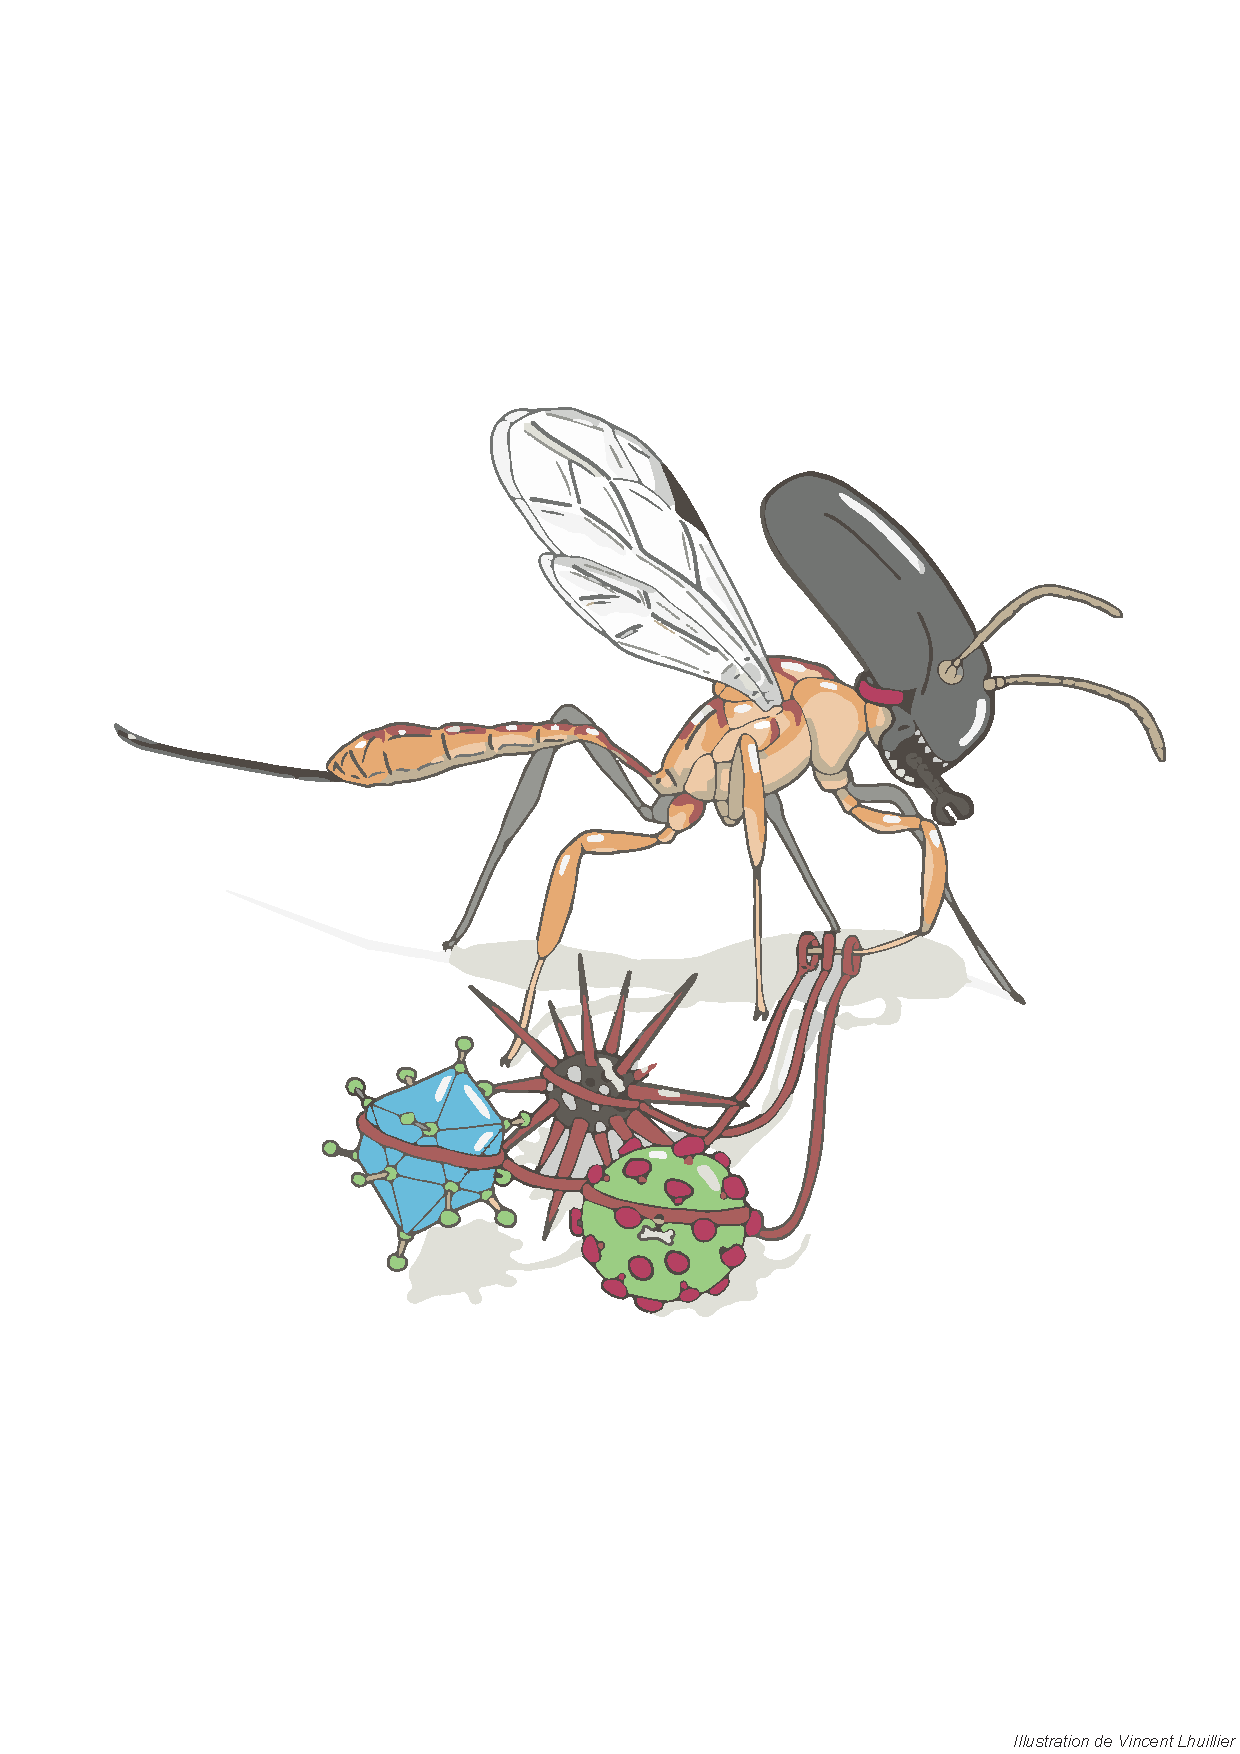
\includegraphics[valign=t,width=1\textwidth, page=1] {figures/preface3}
        \end{center}
        \restoregeometry
    \end{alwayssingle}
    
    \pagestyle{fancybook}

    \part{Introduction}

    \label{part:intro}
    \thispagestyle{empty}
\chapter{Contexte général de la thèse}
{\hypersetup{linkcolor=GREYDARK}\minitoc}
\label{chap:intro-Context}
\newpage

Le cœur de ce projet s'inscrit dans la découverte antérieure de phénomènes de domestication virale chez plusieurs espèces de guêpes dont la progéniture se développe à l'intérieur du corps d'autres insectes; ces insectes étant qualifiés d'endoparasitoïdes. Ces virus sont utilisés aujourd’hui par les guêpes pour administrer des facteurs de virulence essentiels au succès développemental de leur progéniture. Au début de la thèse, cinq événements indépendants de domestication de virus avaient été documentés, dont quatre concernaient une seule super-famille de l’ordre des Hymenoptères (Ichneumonoidea), qui a focalisé l’attention des chercheurs.euses. Puisque ces événements s'étaient répétés à plusieurs reprises, la capacité de produire des particules virales devait conférer un avantage important sur le plan évolutif et jouer un rôle essentiel dans le succès écologique des espèces endoparasitoïdes. Néanmoins, à ce stade, nous manquions d’une vision globale de la fréquence de ces phénomènes de domestication de virus au sein de l’immense diversité des Hyménoptères parasitoïdes. En effet, jusqu'alors, par l'implication de ces espèces dans la lutte contre les ravageurs de cultures, seulement quelques espèces de la super-famille des Ichneumonoidea avaient été séquencées et étudiées, ce qui soulevait clairement un biais dans l'effort d'échantillonnage au sein de la diversité des Hyménoptères. Par exemple, la super-famille des Chalcidoidea est l'une des plus diversifiées au sein des Hyménoptères, en concurrence avec les Ichneumonoidea, avec plus de 22 500 espèces existantes décrites et une estimation allant jusqu'à 500 000 espèces \citep{heraty_phylogenetic_2013}. \\

Le présent projet de thèse vise à rechercher des facteurs qui pourraient structurer les évènements d'endogenisation et de domestication à l'échelle des Hyménoptères. Pour cela, nous analysons un maximum de diversité et incluons des facteurs biologiques différents (espèces endoparasitoïdes, ectoparasitoïdes, et libres) au sein des Hyménoptères, et ceci en utilisant des génomes présents dans les bases de données publiques et séquencées par notre laboratoire.  J'ai  donc développé un pipeline bio-informatique permettant de rechercher de nouveaux cas d'endogénisation et de domestication, et par ailleurs de tester l'existence de facteurs explicatifs  associés à l'apparition de ces phénomènes.\\

En travaillant sur mon projet principal, j'ai fait des découvertes inattendues, ce qui est un événement courant en science. Lors du criblage d'éléments viraux endogènes dans les assemblages de centaines d'espèces d'Hyménoptères, nous avons découvert la présence de virus libres non identifiés chez certaines. Au même moment, une équipe de l'IRBI (Institut de Recherche sur la Biologie de l'Insecte) de Tours faisait également des découvertes connexes chez des virus filamenteux apparentés. Ces travaux ont donc conduit à un projet commun entre nos deux équipes et m'ont offert l'opportunité de décrire une nouvelle famille de virus, tout en apprenant de nouveaux concepts.\\

Enfin, j'ai pu combiner nombre d'idées et de résultats issus de mes deux projets précédents pour le dernier projet de cette thèse. L'objectif de celui-ci était de fournir un compte rendu détaillé de la domestication virale qui s'est produite chez les guêpes endoparasitoïdes du genre \textit{Leptopilina}. C'est lors de ce projet que j'ai pu mettre un pied dans le domaine de la biologie moléculaire en effectuant l'extraction d'ADN et la recherche par PCR d'éléments viraux endogènes sur une quarantaine d'échantillons provenant d'espèces proches des \textit{Leptopilina}. L'idée était de cribler un maximum de diversité autour des espèces de \textit{Leptopilina} afin de remonter jusqu'à l'évènement ancestral d'endogénisation.
Ces analyses m'ont notamment permis de préciser la date à laquelle ces gènes d'origine virale ont été acquis par ces guêpes, puis d'inférer la longue histoire évolutive de la nouvelle famille de virus décrite précédemment. \\

Ce travail de thèse est le fruit de nombreuses collaborations, qu'elles soient techniques via le séquençage de nombreux génomes, participatives grâce au partage de nombreux spécimens, développementales à travers la conception de scripts bioinformatiques, ou bien intellectuelles par les échanges au cours de nombreuses discussions. Aussi, ce voyage n’aurait jamais été si passionnant sans l'aide des nombreuses personnes impliquées de près ou de loin dans ma thèse.\\

Cette thèse est présentée en vue de satisfaire aux exigences du diplôme de Docteur à l'Université de Lyon. Les recherches présentées ici ont été conduites au Laboratoire de Biométrie et de Biologie Évolutive (LBBE), sous la supervision du Maître de conférence, Dr. Julien Varaldi. La thèse est un recueil de trois manuscrits précédés d'une introduction qui les met en relation et fournit des informations générales, suivie finalement d'une discussion générale et d'une mise en perspective de mon travail.\\

Ce travail a été réalisé en utilisant les ressources informatiques du CC LBBE/PRABI ainsi que de l'IFB Biosphère. \\

\newline


\newcolumntype{C}[1]{>{\centering\let\newline\\\arraybackslash\hspace{0pt}}m{#1}}
\newcolumntype{L}[1]{>{\raggedright\let\newline\\\arraybackslash\hspace{0pt}}m{#1}}

    \begin{tabular}{C{2.8cm}  L{5.5cm}}
        \includegraphics[width=\linewidth]{PhD-master/figures/GitHub-logo.png} & Toutes les figures, les scripts et le code source LATEX utilisés dans ce manuscrit peuvent être réutilisés sous licence CC-BY-SA, disponible à l'adresse : \newline
        \href{https://github.com/BenjaminGuinet/PhD_defense}{https://github.com/BenjaminGuinet/PhD\_defense}
    \end{tabular}

    \thispagestyle{empty}
\chapter{Paléovirologie et étude des éléments viraux endogénisés}
{\hypersetup{linkcolor=GREYDARK}\minitoc}
\label{chap:intro-EVES_dEVEs}
\newpage

\section{Le monde singulier des virus}

\subsection{La biologie des virus}

À ma connaissance, toutes les formes de vie cellulaire ont des génomes à ADN double brins (dsDNA) et suivent les mêmes règles de réplication et d'expression. Les virus, quant à eux, utilisent toutes les structures génomiques possibles (\figurename{\ref{figure:Structures_genomiques_virale}}). En effet, les virus ont des génomes constitués d'ADN ou d'ARN, circulaires ou linéaires, et constitués d'une ou plusieurs molécules. 

\begin{figure}[!htpb]
\captionsetup{font=footnotesize}
 \centering
  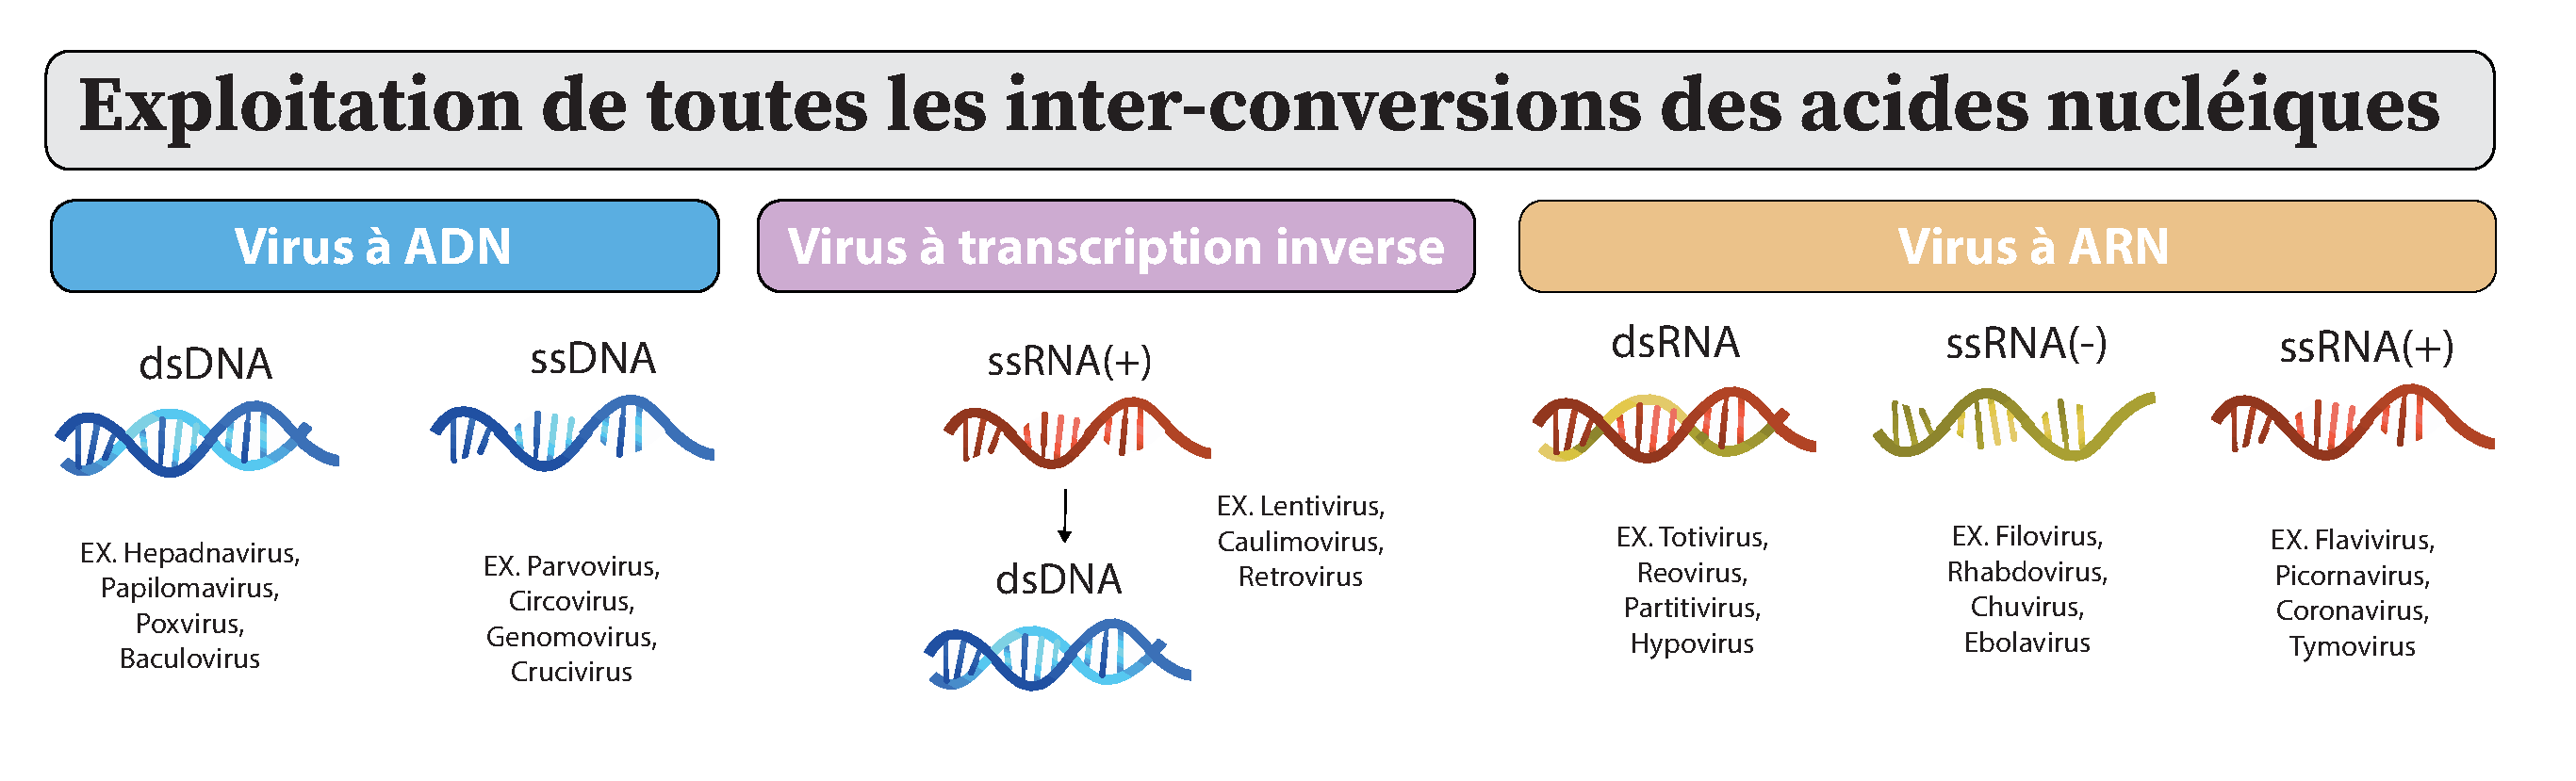
\includegraphics[width=\linewidth,height=\textheight,keepaspectratio]{PhD-master/figures/Structures_genomiques_virales.pdf}
\caption[Intro:Schéma récapitulatif de toutes les structures génomiques virales]{\textbf{Schéma récapitulatif de toutes les structures génomiques virales} }
\label{figure:Structures_genomiques_virale}
\end{figure}

Tous les virus sont des parasites intracellulaires obligatoires, ce qui signifie qu'ils produisent de nouvelles particules virales infectieuses, ou virions, à l'intérieur de la cellule. Bien entendu, les virus ont de nombreuses stratégies d'infection et des biologies différentes, mais il existe quelques généralités. Pour pénétrer dans une cellule, tous les virus doivent par exemple se lier à sa surface. Le virus se décapside alors et son matériel génétique, qui code pour des protéines, va spontanément former de nouveaux virions, après un cycle de réplication \textit{de novo}. Contrairement aux cellules, qui se divisent en deux pour se répliquer, les virus utilisent l'énergie et la machinerie de la cellule pour créer et assembler de nouveaux virions.

Pour infecter d'autres cellules, la particule virale mature doit s'échapper de la cellule hôte. Qu'il s'agisse de virus dsDNA, ssDNA, dsRNA ou ssRNA, le génome du virus évolue dans un environnement hostile. La capside (\figurename{\ref{figure:Structure_virale}}) protège donc l'acide nucléique de tous les virus. Chez certains virus, une enveloppe lipidique protège également la capside (\figurename{\ref{figure:Structure_virale}}). La couche la plus externe de chaque virus contient des protéines d'attachement qui lui permettent, grâce à leur capacité fusogénique, de se fixer à la membrane plasmique de la cellule hôte et de finalement fusionner leurs membranes. Cette fusion membranaire permet au virus de pénétrer dans la cellule. 


\begin{figure}[!htpb]
\captionsetup{font=footnotesize}
 \centering
  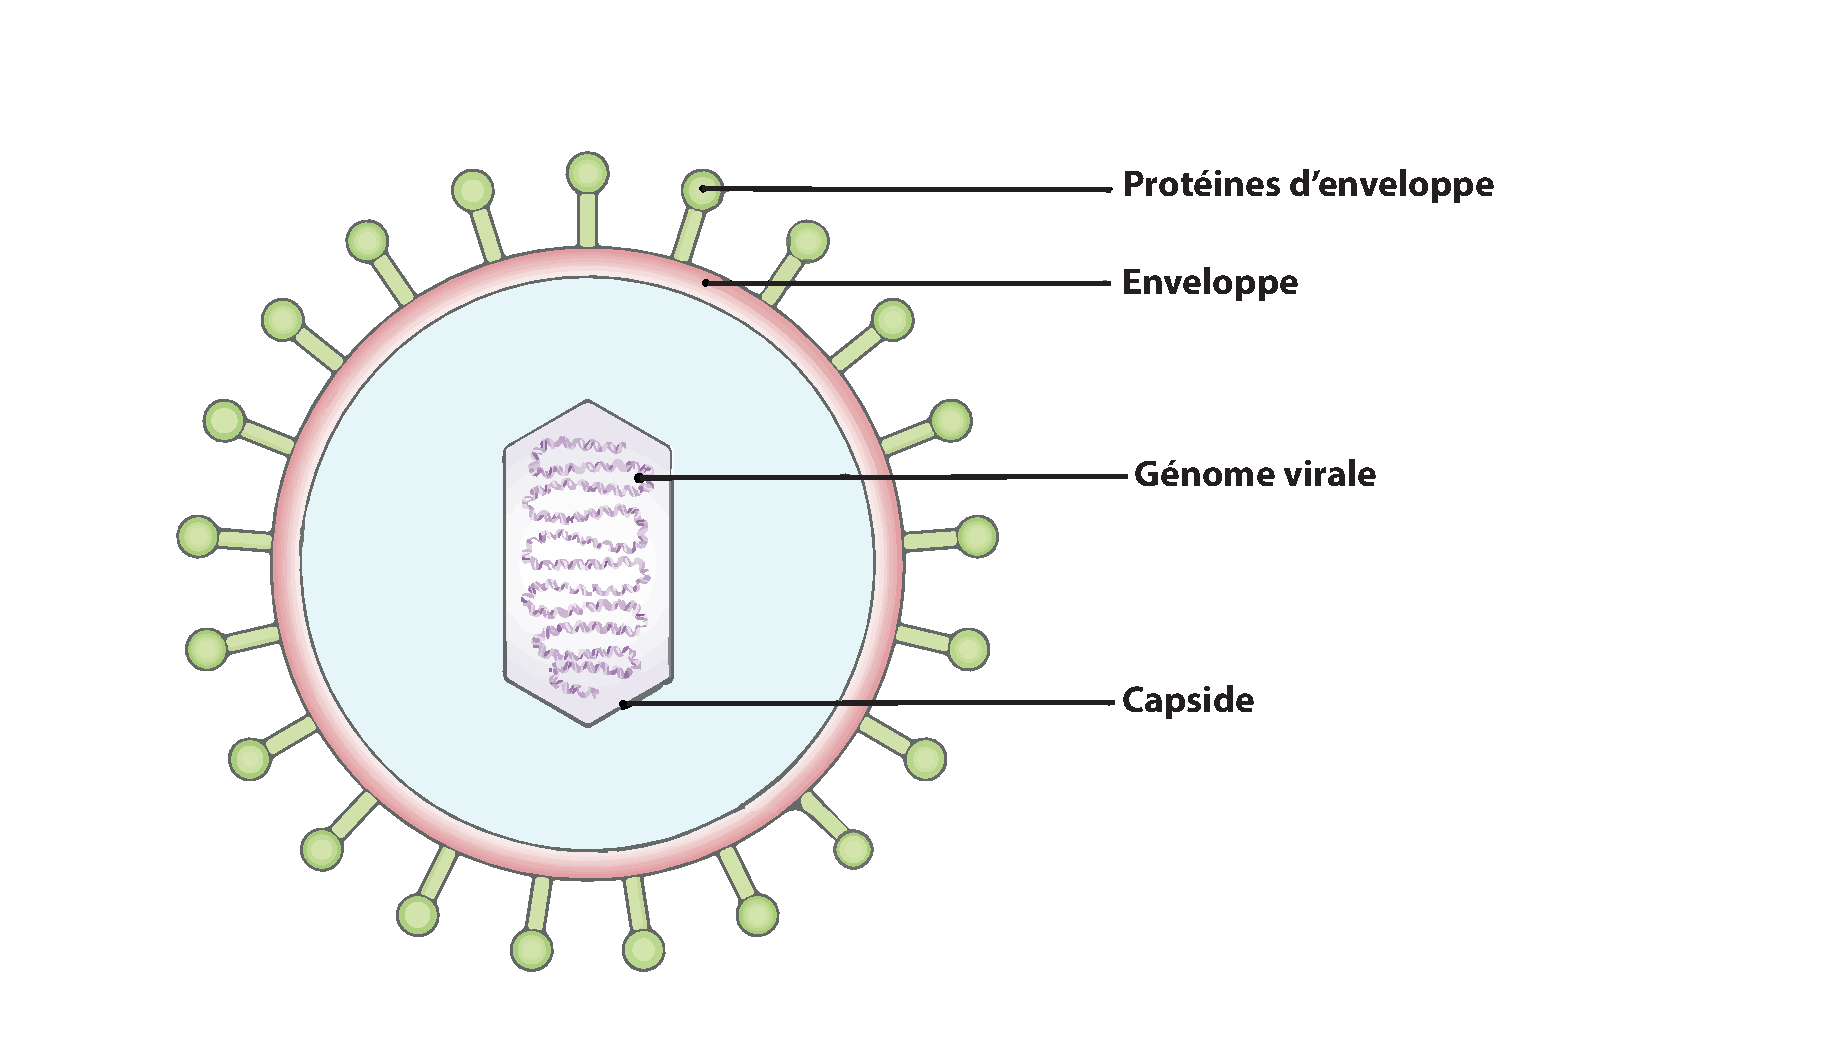
\includegraphics[width=\linewidth,height=\textheight,keepaspectratio]{PhD-master/figures/Structure_virale.pdf}
\caption[Intro:Structure virale générale]{\textbf{Structure virale générale}.}
\label{figure:Structure_virale}
\end{figure}

Contrairement aux génomes cellulaires, les génomes viraux sont très petits (\figurename{\ref{figure:Taille_et_mutations_virales}}). Ainsi, les virus à ARN possèdent les génomes les plus petits (la longueur moyenne du génome de virus ARN le plus petit n'est que de 9kb). Ces petits génomes présentent souvent des taux de mutation plus élevés (\figurename{\ref{figure:Taille_et_mutations_virales}}) \citep{gago_extremely_2009}.

\begin{figure}[!htpb]
\captionsetup{font=footnotesize}
 \centering
  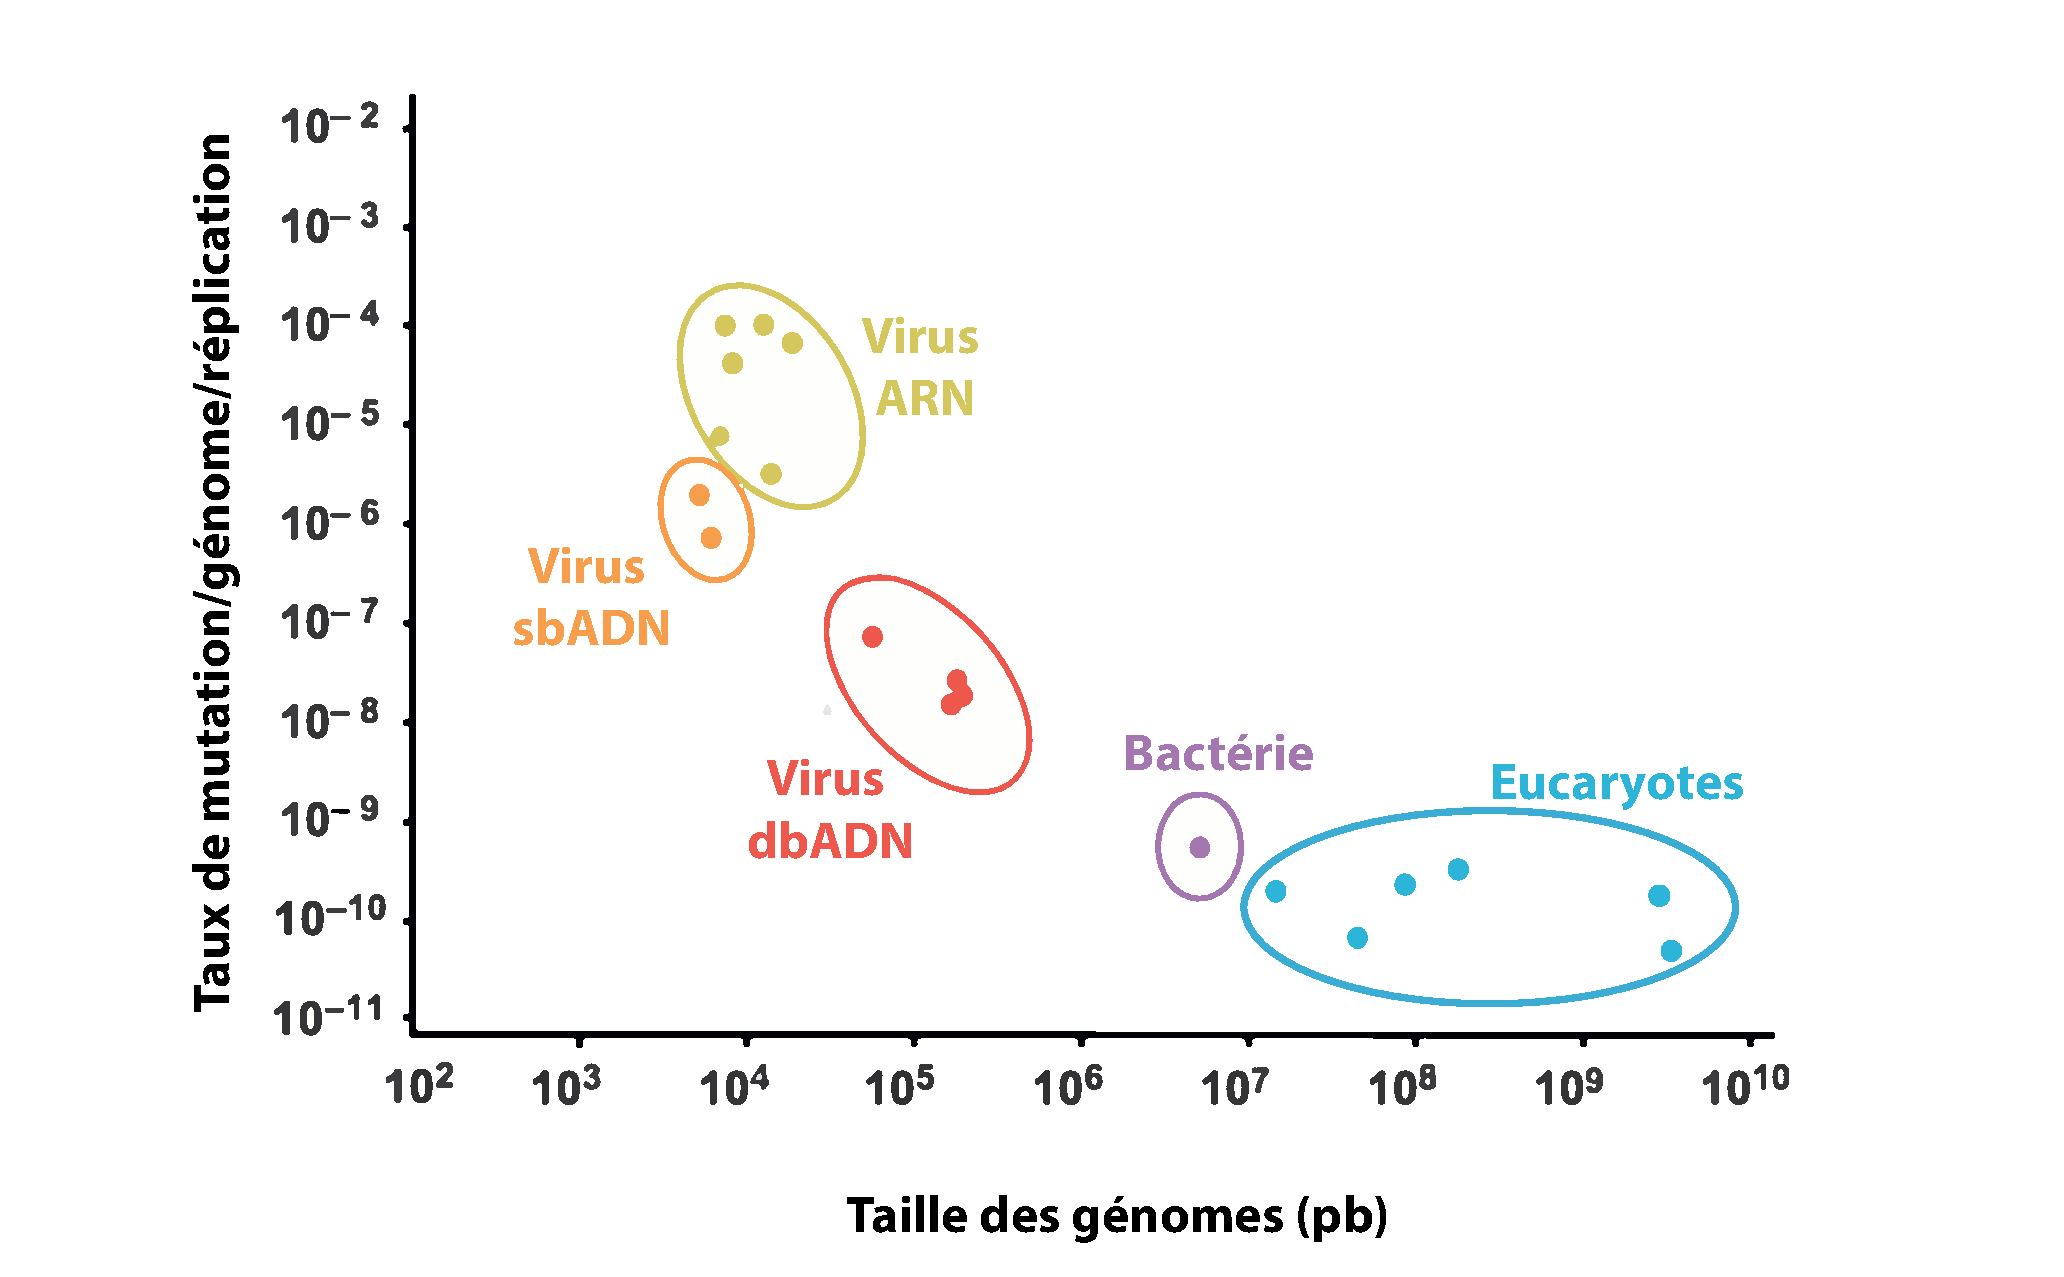
\includegraphics[width=\linewidth,height=\textheight,keepaspectratio]{PhD-master/figures/Taille_et_mutations_virales.pdf}
\caption[Intro:Distribution des taux de mutation en fonction de la taille du génome]{\textbf{Taux de mutation par site en fonction de la taille du génome pour différentes entités biologiques modifié de \cite{gago_extremely_2009}}.}
\label{figure:Taille_et_mutations_virales}
\end{figure}


\subsection{La symbiose}


Les associations symbiotiques entre les symbiotes et leurs hôtes fluctuent selon un continuum allant du parasitisme jusqu’au mutualisme. À ce titre, les virus sont par définition des symbiotes dans la mesure où ils se reproduisent aux dépens d'une cellule hôte. En conséquence, l'évolution de la virulence des virus peut être abordée à la lumière des modèles généraux qui ont été développés sur d'autres modèles symbiotiques, en particulier bactériens. Dans ce modèle, on définit la virulence comment étant la réduction de fitness induite par le symbiote sur son hôte. L'évolution de la virulence est alors principalement gouvernée par le mode de transmission des symbiotes \citep{smith_geneseye_2007}. En cas de transmission horizontale, la sélection est susceptible de favoriser des symbiotes virulents du fait de ce découplage entre les fitness des symbiotes et  de leurs hôtes. À l'inverse, une transmission verticale des symbiotes des parents hôtes à leur progéniture sélectionnera plutôt des symbiotes de moindre virulence, voir ayant un effet bénéfique sur la fitness de leurs hôtes. Dans ce dernier cas, on parle de mutualisme.

Les virus ont tous en général une composante horizontale pour leur transmission, ce qui va favoriser l'évolution de la virulence. Cette virulence peut être forte comme dans le cas du virus Ebola qui se transmet très efficacement entre individus et induit un taux de mortalité très élevé à son hôte \citep{kadanali_overview_2016}. 

En dehors de ces virus à transfert horizontal, d'autres virus présentent à la fois des modes de transmission horizontaux et également verticaux. Dans ce cas-là, la fitness du virus est donc en grande partie liée à son hôte, ce qui sélectionne pour une moindre virulence. Un tel exemple peut être retrouvé chez le virus LbFV (pour Leptopilina boulardi filamentous virus)  qui infecte la guêpe parasitoïde \textit{Leptopilina boulardi}. Ces virus sont transmis principalement verticalement de la mère aux progénitures. Cependant, des transferts horizontaux sont également observés. En effet, LbFV manipule le comportement de ponte des guêpes \textit{Leptopilina boulardi} en induisant du superparasitisme (ponte des œufs chez des hôtes déjà parasités) \citep{varaldi_infectious_2003,varaldi_artifical_2006}. Cette modification comportementale favorise ainsi la transmission horizontale du virus au sein des hôtes diptères superparasités, permettant une propagation efficace du virus dans les populations de guêpes \citep{gandon_superparasitism_2006}. 

Enfin, certains virus présentent plutôt une relation mutualiste avec leurs hôtes, comme le cas d'un entomopoxvirus se répliquant dans la guêpe parasitoïde \textit{Diachasmimorpha longicaudata} (DlEPV). Ce virus mutualiste est transmis verticalement et donne aux guêpes \textit{D. longicaudata} un avantage en termes de fitness en favorisant le succès reproducteur lors d'une infestation chez un hôte diptère \citep{coffman_genomic_2020}. Enfin, il existe également une forme de mutualisme plus poussée - on pourrait même parler d'un paroxysme symbiotique - qui implique les virus sous une forme intégrée dans les génomes de leurs hôtes (éléments viraux endogènes ou EVEs), comme dans le cas du gène d'enveloppe \textit{env} de rétrovirus, endogène chez les mammifères, qui permet la formation du syncitium \citep{lavialle_paleovirology_2013}.

\section{Les Éléments viraux endogènes (EVEs)}

\subsection{Historique}

Outre leurs propriétés infectieuses qui permettent aux virus de se propager de manière horizontale entre individus et entre espèces, il peut arriver qu'un virus s'intègre au matériel génétique de l'hôte via un processus connu sous le nom d'endogénisation \citep{katzourakis_endogenous_2010}. Ce phénomène d'endogénisation génère l'apparition de ce qu'on appelle des "Endogenous Viral Elements", en français "Eléments Viraux Endogènes" (EVEs). Les intégrations virales dans les chromosomes de leurs hôtes  peuvent alors concerner de petits fragments de génomes viraux, jusqu'à des génomes viraux entiers \citep{feschotte_endogenous_2012}.\\

Les premières recherches sur les EVEs ont principalement porté sur les rétrovirus endogènes (\textit{Retroviridae}), abondants dans les génomes des vertébrés et des plantes \citep{johnson_origins_2019}. Si la majeure partie des EVEs retrouvés dans la littérature correspond à des intégrations virales provenant de rétrovirus, c'est notamment parce qu'il s'agit des seuls virus à nécessiter une intégration chromosomique pour réaliser leur cycle de vie complet. Cette propriété dérive du fait que leur génome code pour l'ensemble de la machinerie enzymatique nécessaire à l'intégration. Ainsi, lorsque les particules composées de copies d'ARN du génome viral pénètrent dans une cellule cible, elles sont retro-transcrites en une molécule d'ADN double brin et intégrées à l'ADN génomique de la cellule hôte. Le provirus qui en résulte (forme intégrée, aussi appelée ERV pour endogenous retrovirus) code toutes les protéines structurelles et les enzymes nécessaires à l'assemblage des virions de la progéniture, ainsi que les éléments régulateurs nécessaires à la transcription de l'ARN viral. Les rétrovirus infectent généralement les tissus somatiques et ne sont donc pas transmis aux générations suivantes.  Toutefois, l'intégration peut parfois se produire dans les cellules germinales, permettant la propagation dans une population hôte. Une fois transmises à la génération suivante, ces nouvelles insertions peuvent éventuellement se fixer dans la population, soit par dérive, soit par sélection \citep{johnson_origins_2019}.   

À la fin des années 1990 et au début des années 2000, des EVEs dérivant de virus non retroviraux ont été décrites dans diverses lignées d'eucaryotes \citep{katzourakis_endogenous_2010,belyi_sequences_2010,liu_widespread_2010}. Aussi, l’explosion des programmes de séquençage de génome a permis de révéler la fréquence et la diversité virale impliquée dans ces phénomènes d’endogénisation. Toutes sortes de virus ont pu être endogénisés chez toutes sortes d'organismes, que l’intégration dans les chromosomes de leur hôte fasse partie ou non de leur cycle de vie naturel \citep{feschotte_endogenous_2012,aiewsakun_endogenous_2015}. Chez les insectes par exemple, pour lesquels aucun rétrovirus n'a été décrit jusqu'à aujourd'hui, de nombreux travaux montrent que les génomes abondent d'EVEs non rétroviraux \citep{gilbert_diversity_2022,cheng_nudivirus_2020,flynn_assessing_2019}.\\

Les EVEs non rétroviraux peuvent dériver de virus ayant des génomes dsDNA \citep{di_giovanni_behavior-manipulating_2020,liu_endogenous_2020,katzourakis_origins_2014}, ssDNA \citep{parker_laterally_2019,gibbs_two_2006}, ssRNA \citep{lequime_discovery_2017,flynn_assessing_2019} et dsRNA \citep{horie_endogenous_2010, katzourakis_endogenous_2010, liu_endogenous_2020}. Bien que l'endogénisation de tous ces virus soit inattendue, elle l'est d'autant plus pour les virus à ARN. Dans ce cas, l'endogénisation nécessite trois étapes inhabituelles qui n'interviennent généralement pas dans leur cycle de vie : (i) réverse transcription de l'ARN génomique en ADN, (ii) entrée dans le noyau et (iii) intégration chromosomique dans la lignée germinale. 


\subsection{Mécanismes d'intégrations}

Les mécanismes moléculaires à l'origine des EVEs impliquant des virus non rétroviraux sont beaucoup moins connus que ceux des rétrovirus. 

Concernant les virus à ADN, plusieurs études ont proposé des mécanismes qui font intervenir la jonction entre de l'ADN de l'hôte et l'ADN du virus médiés par la machinerie de réparation des cassures double brins (NHEJ) de la cellule \citep{gilbert_genomic_2010, geering_endogenous_2014}. D'autres études montrent également des cas de recombinaisons homologues comme chez un herpesvirus humains (HHV-6) dont une intégrase permet l'intégration dans les télomères de l'hôte grâce à une homologie de séquence entre des séquences répétées du génome viral et les télomères \citep{arbuckle_latent_2010,osterrieder_herpesvirus_2014}.  

Selon une autre hypothèse, certains virus pourraient s'intégrer en interagissant avec la machinerie de rétrotransposition des cellules \citep{katzourakis_endogenous_2010}. En effet, l'étude de la localisation génomique des EVEs dérivées de virus à génome ARN et de petits virus d'ADN montre qu'ils ont tendance à être enrichis près des rétrotransposons, suggérant qu'une machinerie enzymatique codée par des rétrotransposons dans le génome hôte pourrait être impliquée dans l'intégration d'EVEs, ou alternativement que les EVEs s'intègrent plus, ou sont moins contre-sélectionnés dans ces régions génomiques \citep{katzourakis_endogenous_2010,gilbert_diversity_2022,suzuki_non-retroviral_2020}. 

Enfin, des analyses suggèrent que des rétrotransposons LTR autonomes (tels que IAP) et les rétrotransposons non-LTR autonomes (tels que L1 humain) peuvent également faciliter la transcription inverse ainsi que leur insertion génomique  \citep{geuking_recombination_2009}. Par exemple, la majorité des fragments endogènes de bornavirus présents dans les génomes humains semblent provenir de la transcription inverse et de l'intégration de l'ARNm de la nucléoprotéine (N) d'anciens bornavirus par l'intermédiaire de l'activité LINE-1 \citep{horie_endogenous_2010}.
\newpage

\begin{figure}[!htpb]
\captionsetup{font=footnotesize}
 \centering
  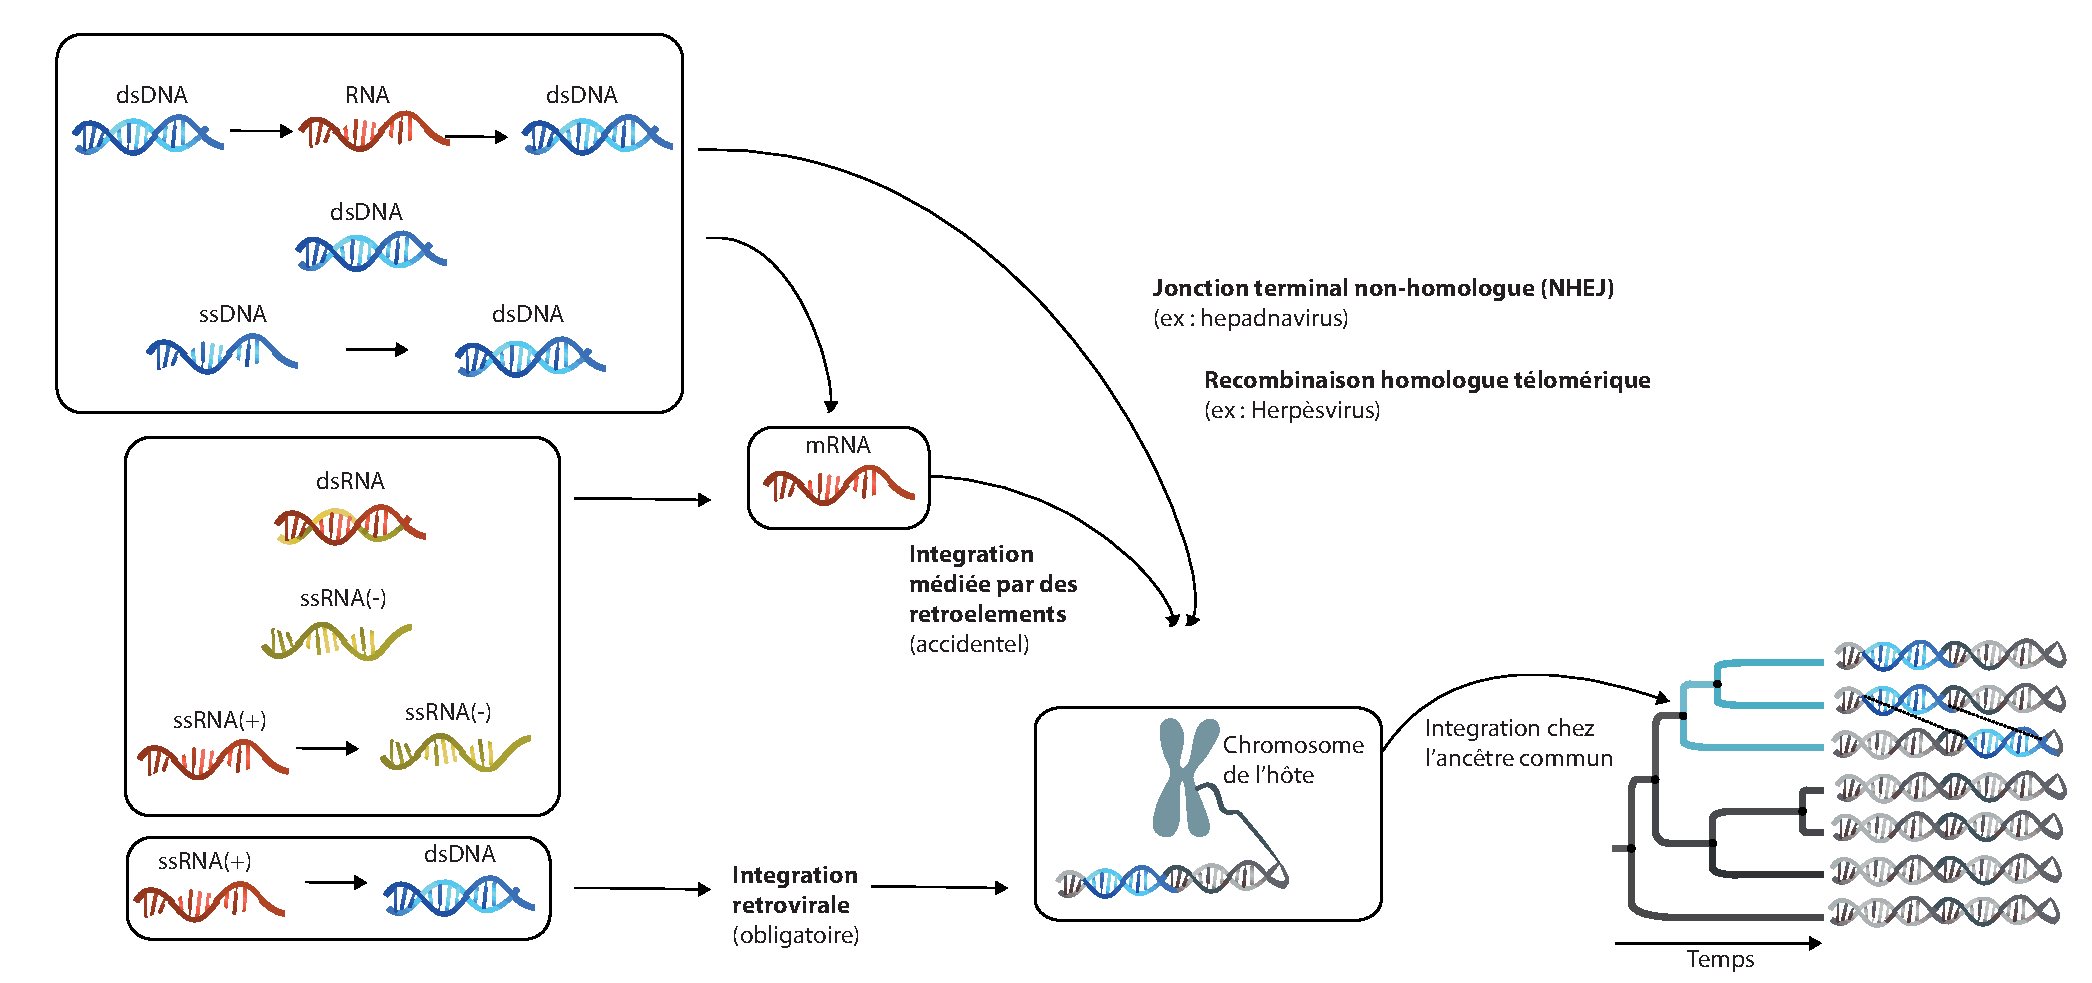
\includegraphics[width=\linewidth,height=\textheight,keepaspectratio]{PhD-master/figures/EVEs.pdf}
\caption[Intro:Schéma récapitulatif d'endogénisation virale]{\textbf{Schéma récapitulatif d'endogénisation virale modifié de \cite{katzourakis_endogenous_2010}}. Lorsqu'un évènement d'endogénisation viral a lieu dans le chromosome d'une cellule germinale d'une espèce, ces EVEs peuvent se voir transmis à la descendance et se fixer dans la population. L'histoire évolutive de ces EVEs doit alors être congruente avec l'histoire évolutive des hôtes. Plus l'évènement est ancien, plus nous pouvons nous attendre à observer des épisodes de réarrangement ou de pertes au cours de l'évolution.}
\label{figure:EVE}
\end{figure}



\subsection{Naissance d'un EVE}

L'apparition des EVEs peut donc survenir suite à l'intégration chromosomique de l'ADN viral (ou de copies d'ADN complémentaires issues d'ARN viraux) médiée par plusieurs mécanismes. Néanmoins, ces évènements sont rares chez les eucaryotes puisque d’une part l’ADN est protégé par un noyau, ce qui rend les contacts entre des éléments génétiques exogènes et le génome plus difficiles, et d’autre part, chez les espèces métazoaires tout au moins, la lignée germinale est habituellement séparée du reste des cellules, un gène acquis chez un métazoaire n’a donc aucune chance d'être fixé dans une population s’il n’atteint pas la lignée germinale. Aussi rares soient-ils, de tels évènements d'intégration germinale peuvent néanmoins survenir, monter en fréquence, puis se fixer dans la population  (\figurename{\ref{figure:EVE}}). Ces fixations peuvent se produire de manière non adaptative, par dérive, ou dans un certain nombre de cas, à la suite de processus adaptatifs. On parle alors de domestication virale que je vais illustrer dans la partie 2.3. 

\subsection{Les EVEs : des fossiles pouvant dater l'histoire ancienne des virus} 

Les séquences génomiques virales accumulent des changements évolutifs à un rythme élevé en raison de leur taux d'évolution élevé. Sur le temps ancien, du fait de la saturation du signal, les séquences virales contemporaines ne portent donc qu'une quantité limitée d'informations. En conséquence, les données virales contemporaines sont souvent insuffisantes pour nous informer sur la façon dont les virus ont évolué et ont interagi avec leurs hôtes dans les temps très anciens. Il n'existe par ailleurs pas de trace fossile de ces virus. Néanmoins, les virus peuvent laisser des empreintes durables dans les génomes de leurs hôtes à travers ces événements d'endogénisation. Après ces évènements, les génomes viraux ne sont plus soumis aux taux de mutation très élevés des virus (\figurename{\ref{figure:Taille_et_mutations_virales}} et \figurename{\ref{figure:Datation_virale_et_taux}}); au contraire, ils sont désormais liés aux génomes de leurs hôtes, dont les taux de mutation sont beaucoup plus faibles \citep{katzourakis_endogenous_2010, feschotte_endogenous_2012} (\figurename{\ref{figure:Datation_virale_et_taux}}). 

\begin{figure}[!htpb]
\captionsetup{font=footnotesize}
 \centering
  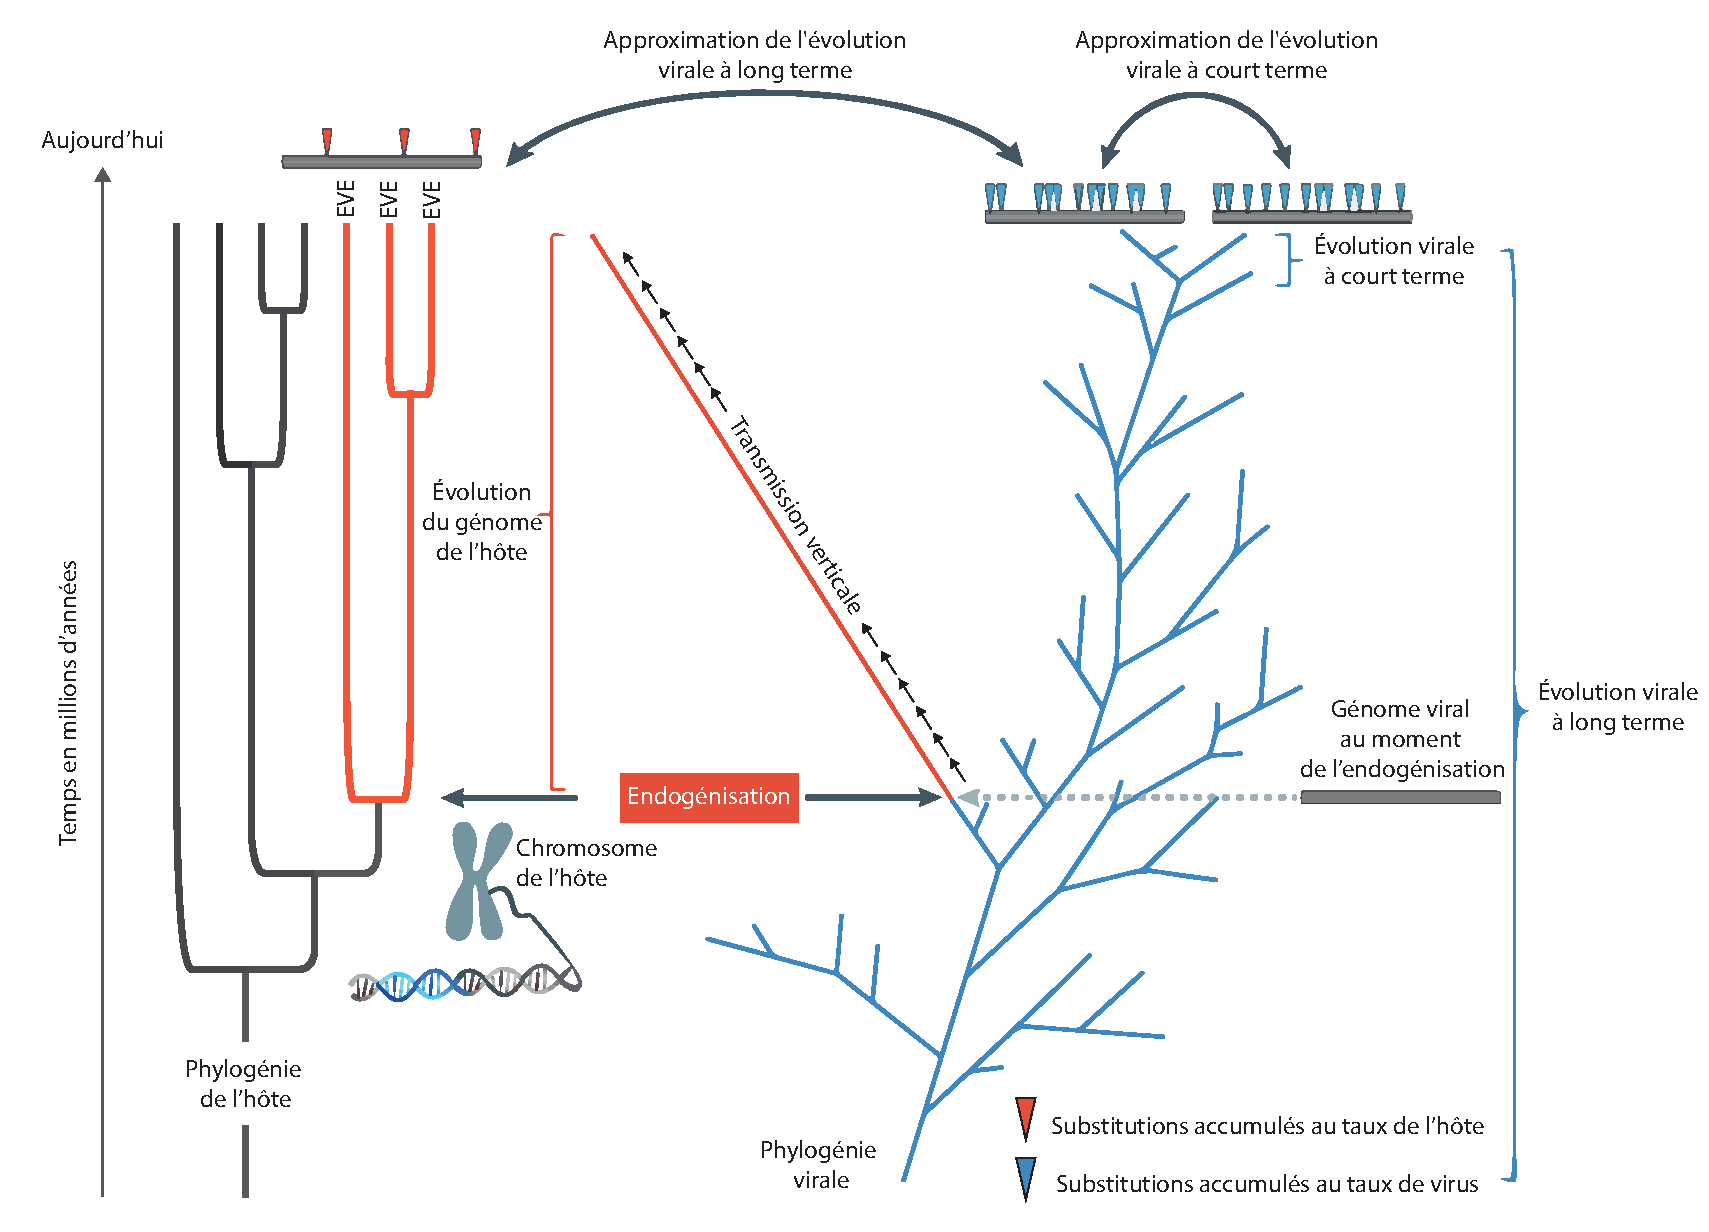
\includegraphics[width=\linewidth,height=\textheight,keepaspectratio]{PhD-master/figures/Datation_virale_et_taux.pdf}
\caption[Intro:Schéma du principe de datation des EVEs ]{\textbf{Datation des EVEs et déduction des taux de substitution virale à long terme modifié de \cite{feschotte_endogenous_2012}}. Lors d'un évènement d'endogénisation d'un virus chez l'ancêtre commun de plusieurs espèces eucaryotes, les séquences intégrées vont se mettre à évoluer au même rythme que les séquences du génome eucaryote (rouge). Tandis que les virus apparentés au donneur de ces EVEs vont eux continuer à évoluer avec de forts taux de mutations (bleu). Si nous voulons dater l'arbre viral, nous pouvons donc utiliser les informations de l'âge relatif des nœuds disponibles dans l'arbre eucaryote récoltés par exemple à partir de fossiles. Ces nœuds peuvent nous permettre de calibrer l'arbre viral puisqu'il existe toujours une relation phylogénétique entre les EVEs et les séquences virales contemporaines.}
\label{figure:Datation_virale_et_taux}
\end{figure}

Les EVEs fixés conservent donc des informations sur la circulation des virus anciens, qu'il est parfois impossible de déduire de l'examen des populations virales contemporaines. Ils fournissent des informations essentielles sur les virus anciens, telles que leur gamme d'hôtes, les échelles de temps d'évolution, ou les répartitions géographiques \citep{gifford_transitional_2008,katzourakis_endogenous_2010}.

Il existe ainsi diverses méthodes qui permettent d'utiliser les informations provenant des EVEs pour donner une limite inférieure sur l'âge des familles virales concernées \citep{aiewsakun_endogenous_2015}. L'une d'entre elle, applicable à tous les types de virus endogènes, consiste à exploiter les informations provenant d'EVEs orthologues (c'est-à-dire des EVEs hérités d'un ancêtre commun). Si la date de spéciation de ces espèces hôtes est par ailleurs connue grâce à des registres fossiles, il est alors possible de déduire que la date d'intégration du virus est antérieure à la spéciation des espèces hôtes concernées. 

Les lentivirus, par exemple, ont initialement été considérés comme un groupe de virus d'évolution récente, sur la base des origines très récentes du VIH-1 et des taux de substitution mesurés qui situent les origines des lentivirus à quelques milliers d'années \citep{sharp_origins_2000}. Pourtant, des chercheur.euse.s ont pu observer la présence de lentivirus endogénisés partagés dans des génomes apparentés de lapins, de furets, de lémuriens de Madagascar et de Colugos soutenant l'hypothèse d'une circulation de ces virus chez l'ancêtre de ces différents organismes, plusieurs millions d'années en arrière donc \citep{hron_life_2016,katzourakis_discovery_2007}. D'autres exemples analogues abondent comme chez les filovirus, parvovirus, circovirus, bornavirus, pestivirus, flavivirus qui circulaient déjà, il y a des millions d'années, au cours de l'évolution des mammifères, d'après leur distribution dans les espèces contemporaines \citep{katzourakis_endogenous_2010,taylor_filoviruses_2010,li_endogenous_2022}.

\begin{figure}[!htpb]
\captionsetup{font=footnotesize}
 \centering
  \includegraphics[width=\linewidth,height=\textheight,keepaspectratio]{PhD-master/figures/Datation_virale_scheme.pdf}
\caption[Intro:exemple de datation virale à partir d'EVEs]{\textbf{exemple d'une phylogénie virale calibrée à partir de virus domestiqués modifié de \cite{theze_paleozoic_2011}}. Dans cet exemple, la phylogénie des virus à grand génome à ADN double brin infectant les arthropodes de la classe des \textit{Naldaviricetes} a pu être calibrée grâce à un évènement d'endogénisation ayant eu lieu y a environ 100 millions d'années chez l'ancêtre commun des guêpes parasitoïdes appartenant au complexe des Microgastroïdes.}
\label{figure:Datation_virale_scheme}
\end{figure}

Dans un autre exemple, \cite{theze_paleozoic_2011} ont  pu exploiter les EVEs partagés par plusieurs milliers d'espèces d'Hymenoptères parasitoïdes (le complexe microgastroïde au sein des Braconidae) pour calibrer la phylogénie des virus donneurs (\figurename{\ref{figure:Datation_virale_scheme}}). Cette calibration permet en retour de dater la divergence de la famille de virus. En effet, grâce à l'étude de \citep{murphy_phylogeny_2008}, les chercheur.euses savaient que le temps jusqu'à l'ancêtre commun le plus récent de l'espèce \textit{Chelonus inanitus} et de \textit{Cotesia congregata} était égal à 103,38 +/- 4,41 Mya (correspondant au nœud 2 dans la \figurename{\ref{figure:Datation_virale_scheme}}). De même, ils savaient que l'ancêtre commun de \textit{Cotesia congregata} et de \textit{Toxoneuron nigriceps} était estimé à environ 87 +/- 5 Mya (nœud 1 dans la \figurename{\ref{figure:Datation_virale_scheme}}). Aussi, sur la base de ces estimations provenant de registres fossiles, ces points de calibration dans l'arbre de l'hôte (point 1 et 2) peuvent également servir de point de calibration dans l'arbre des virus (point 1 et 2) (\figurename{\ref{figure:Datation_virale_scheme}}). Une fois l'arbre viral calibré, la divergence entre la famille des \textit{Baculoviridae} et celle des \textit{Nudiviridae} a pu être estimée. Ces analyses révèlent que les virus dsDNA des insectes (ici représentés par les \textit{Nudiviridae} et \textit{Baculoviridae}) se seraient diversifiés il y a environ 310 Mya à l'ère paléozoïque, pendant la période carbonifère, ce qui coïncide avec la période de diversification des premiers ordres d'insectes \citep{theze_paleozoic_2011}. 

\section{Les Éléments viraux endogènes domestiqués (dEVEs)}

Quel est le devenir des éléments endogénisés ? La dégénérescence est probablement le destin le plus fréquent des EVEs, puisqu'il s'agit d'un évènement de mutation accidentel qui n'apporte \textit{a priori} aucun bénéfice pour l'hôte. En effet, de nombreux EVEs identifiés ont accumulé un grand nombre de mutations depuis leur intégration et/ou sont fragmentés : ils représentent probablement des pseudogènes non fonctionnels, évoluant sous un régime neutre \citep{katzourakis_endogenous_2010}. Cependant, l'endogénisation de séquences virales dans le génome de l'hôte peut parfois être bénéfique pour l'hôte et entraîner une fixation de l'élément viral endogène dans les populations à travers un phénomène de sélection positive.  On parle alors de domestication et les EVES sont qualifiés de dEVEs (pour domesticated Endogenous Viral Elements) \citep{koonin_depths_2018}. Ainsi, l'introduction d'un ou plusieurs gènes viraux dans les génomes eucaryotes représente un input mutationnel à fort impact. En effet, ces mutations peuvent être vues comme des "macro-mutations" dans la mesure où un ou plusieurs gènes déjà fonctionnels et façonnés par la sélection naturelle sont intégrés, ce qui offre de nombreuses possibilités de domestication par l'hôte. Les travaux sur la domestication des EVEs ont permis d'identifier de nombreuses fonctions recrutées par les eucaryotes, telles que des fonctions de communication et d'échanges métaboliques, de défenses antivirales, de plasticité phénotypique ou bien les interactions hôtes-parasites. 

\subsection{Développement placentaire}

Les exemples les mieux étudiés jusqu'à présent sont les protéines syncytines. Ces protéines retrouvées chez tous les mammifères placentaires sont dérivées de protéines \textit{env} présentes chez des rétrovirus. Les rétrovirus ciblent, se fixent et intègrent les membranes des cellules cibles en exprimant le gène \textit{env} (Coffin JM et al., 1997). Ces protéines ont des propriétés fusogéniques et permettent aux virus de se lier aux celles de leurs hôtes. De manière remarquable, cette protéine a été domestiquée à plusieurs reprises chez plusieurs lignées de mammifères et de lézards vivipares et permet la formation du syncitium en médian une fusion entre les cellules de la mère et de l'embryon permettant les échanges métaboliques entre la mère et le fœtus (\figurename{\ref{figure:Syncitine_illustration}}-A) \citep{lavialle_paleovirology_2013,cornelis_endogenous_2017}. En effet, ces gènes sont domestiqués dans toute la sous-classe des thériens, avec au moins dix événements d'intégration rétrovirale indépendants \citep{imakawa_baton_2015}(\figurename{\ref{figure:Syncitine_illustration}}-B).\\

De manière surprenante, les propriétés fusogéniques des syncytines semblent également avoir été  utilisées pour soutenir le développement musculaire, car le knock-out de la syncytine B chez les souris entraîne une diminution de la fusion des myoblastes et de la masse musculaire chez les mâles \citep{redelsperger_genetic_2016}. Ces résultats montrent comment les propriétés biochimiques des enveloppes virales ont été recyclées plusieurs fois au cours de l'évolution.

\begin{figure}[H]
\captionsetup{font=footnotesize}
 \centering
  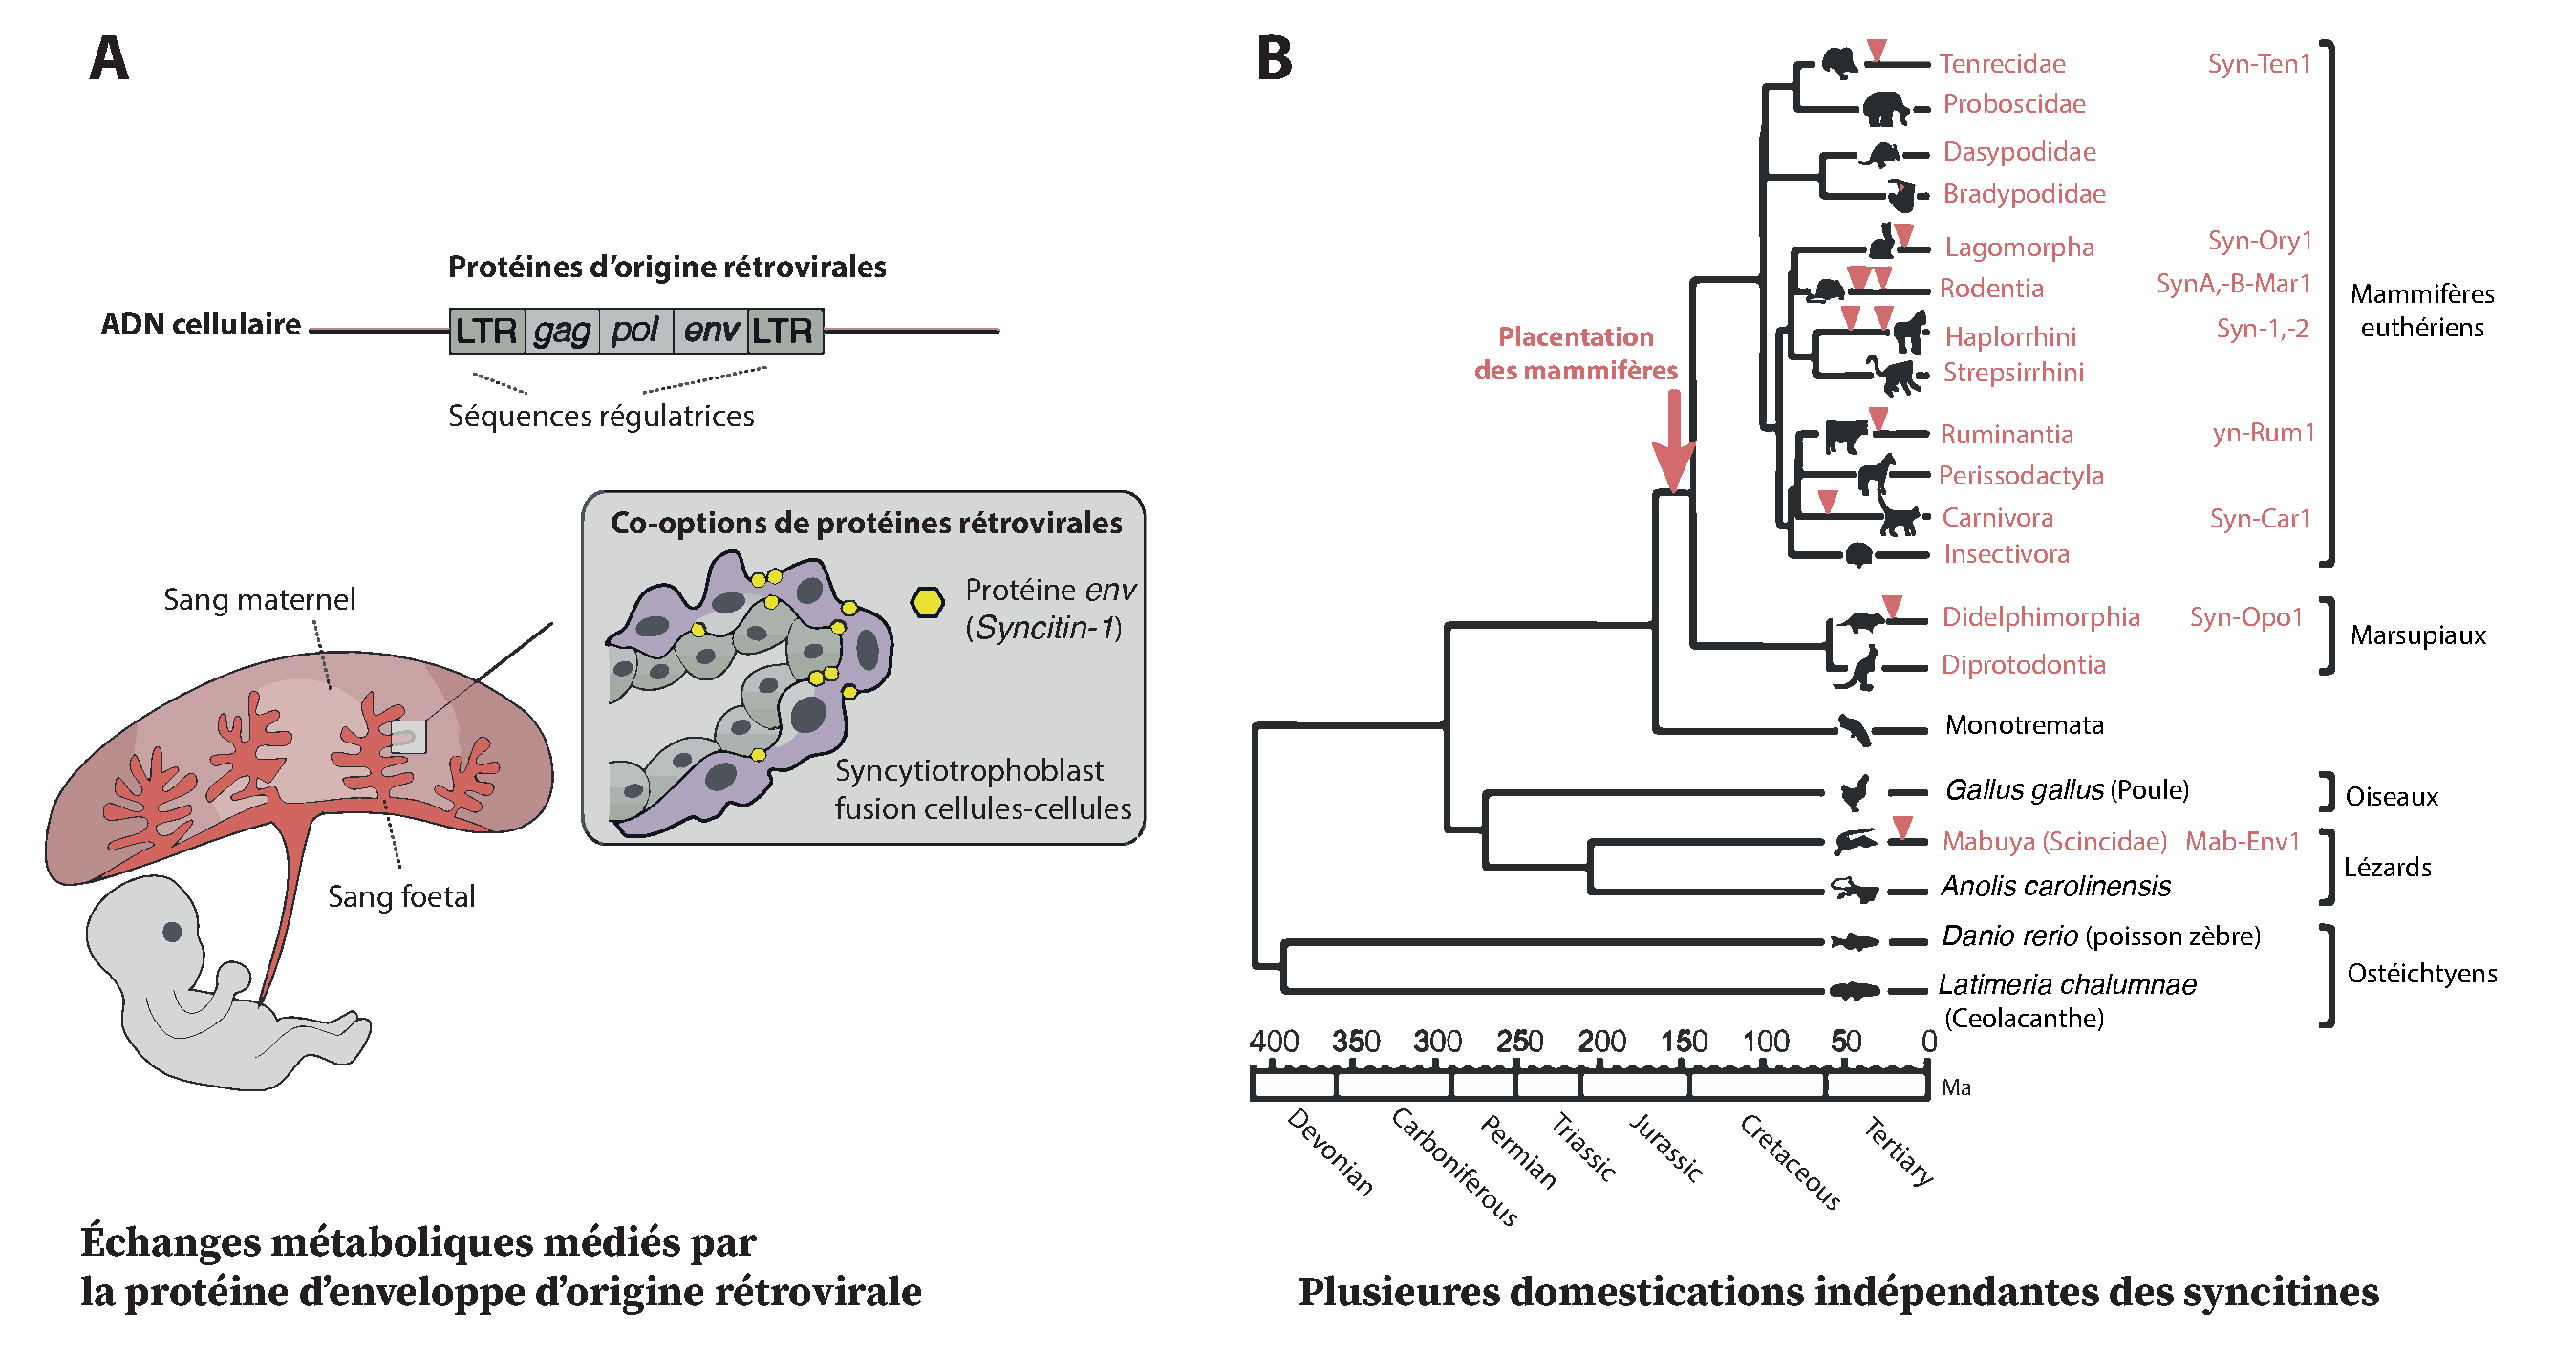
\includegraphics[width=\linewidth,height=\textheight,keepaspectratio]{PhD-master/figures/Syncitine_illustration.pdf}
\caption[Intro:Illustration d'un gène de rétrovirus impliqué dans la production du syncitium chez les mammifères placentaires]{\textbf{Exemple schématique de la domestication d'un gène rétroviral impliqué dans la formation du syncytium modifié de} \cite{chuong_placenta_2018, cornelis_endogenous_2017}. \textbf{A} -  Exemple schématique de la fonction fusogénique des syncitines dans la formation du syncytiophoblast ainsi que la disposition des gènes rétroviraux et de séquences régulatrices le long du génome d'un mammifère. \textbf{B} -  Classification des mammifères, du lézard \textit{Mabuya} et des syncytines connues selon la phylogénie des vertébrés. Les mammifères comprennent les monotrèmes (p. ex. l'ornithorynque) qui produisent encore des œufs, ainsi que les marsupiaux et les mammifères euthériens qui ont un placenta (caractères rouges). Le lézard \textit{Mabuya} est représenté en rouge, car il porte lui aussi un placenta. Une flèche rouge marque la période probable de formation du placenta des mammifères, qui a été supposée correspondre à la capture d'une syncytine ancestrale, qui a ensuite été remplacée par les syncytines actuelles présentées. Toutes les occurrences de capture de syncytine actuellement décrites sont indiquées par des pointes de flèche rouges à côté du nom de la syncytine. Comme l'illustre l'échelle située sous l'arbre, la longueur des branches est liée au temps en millions d'années.}
\label{figure:Syncitine_illustration}
\end{figure}

\subsection{La communication synaptique}

Un autre fait remarquable de domestication virale impliquant des rétrovirus est celui du gène neuronal \textit{Arc}. Ce gène est dérivé d'un rétrotransposon Ty3/Gypsy domestiqué et code un domaine de capside présentant une similarité structurelle avec les protéines rétrovirales. Récemment, il a été  démontré que cette protéine forme des structures de type capside, impliquées dans la fonction neuronale et la mémoire \citep{ashley_retrovirus-like_2018}, Ces protéines, à la façon d'un rétrovirus (\figurename{\ref{figure:Arc_illustration}}-A), s'auto-assemble en capsides de type viral capables d'encapsider de l'ARN (\figurename{\ref{figure:Arc_illustration}}-B). Ces capsides permettent de réguler la plasticité synaptique en médian des échanges synaptiques. Ensuite, la protéine Arc endogène est libérée des neurones dans des vésicules extracellulaires, facilitant le transfert de l'ARNm \textit{Arc} dans de nouvelles cellules musculaires post-synaptiques  où il est traduit en protéine \citep{ashley_retrovirus-like_2018, pastuzyn_neuronal_2018}. 
Tout comme la syncytine chez les mammifères, les gènes \textit{Arc} retrouvés chez les drosophiles et les tétrapodes descendraient de plusieurs évènements d'endogénisation indépendants de rétrotransposons Ty3/gypsy dans des lignées eucaryotes distinctes \citep{pastuzyn_neuronal_2018}. \\

\begin{figure}[H]
\captionsetup{font=footnotesize}
 \centering
  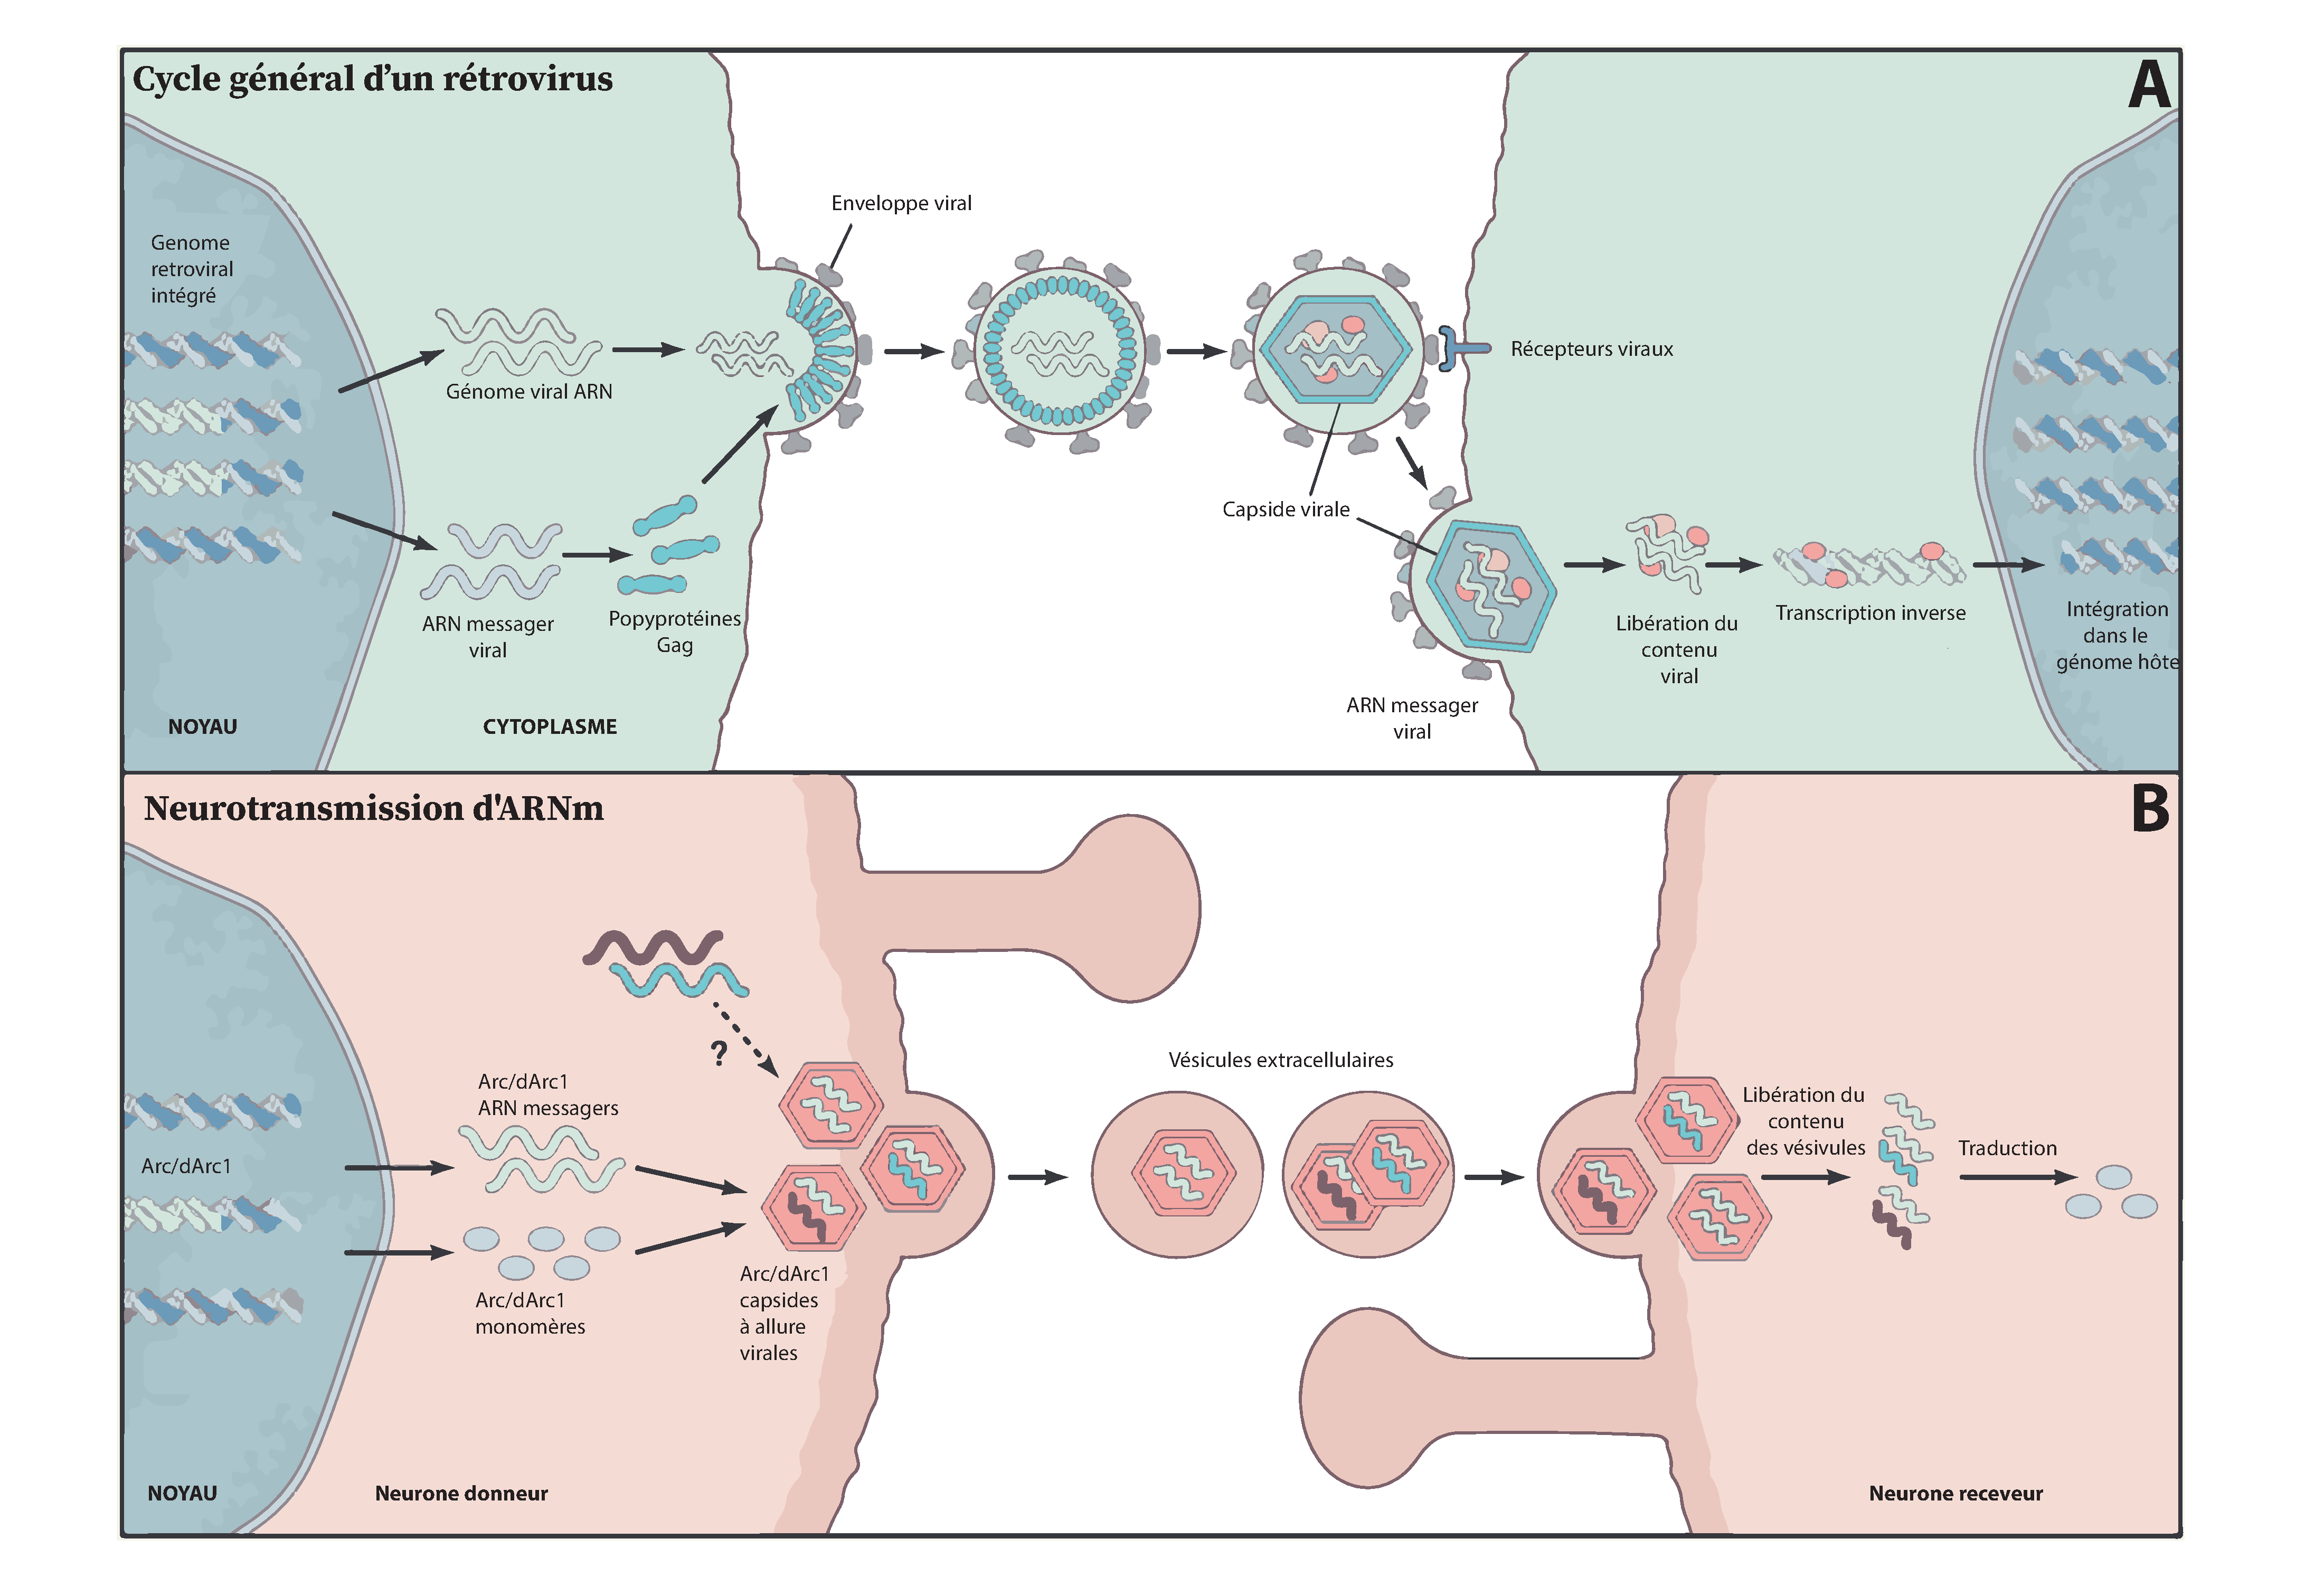
\includegraphics[width=\linewidth,height=\textheight,keepaspectratio]{PhD-master/figures/Arc_illustration.pdf}
\caption[Intro:Illustration de la fonction du gène rétroviral \textit{Arc}]{\textbf{Illustration de la fonction du gène rétroviral \textit{Arc} modifié de \cite{parrish_viral_2018}}. \textbf{A} - Cycle rétroviral classique dans lequel la polyprotéine rétrovirale \textit{Gag} assure la formation de la capside afin de regrouper les génomes viraux et de les transférer dans le cytoplasme des cellules nouvellement infectées. \textbf{B} - L'oligomérisation des protéines \textit{Arc} de souris et \textit{Arc1} de drosophile (\textit{dArc1}) forme des capsides ressemblant à celles des virus. Les capsides \textit{Arc/dArc1} sont libérées des neurones dans des vésicules extracellulaires, où elles transmettent leurs ARNm associés (vert clair) et peut-être des ARN supplémentaires (marron, bleu) à la synapse ou à la jonction neuromusculaire.} 
\label{figure:Arc_illustration}
\end{figure} \newpage

\subsection{Immunité antivirale}

 Le principal mécanisme antiviral chez les arthropodes est l'interférence ARN (ARNi), qui repose sur trois types de petits ARN (ARNs : siARN, miARN et piRNA) \citep{obbard_evolution_2009}. La voie du petit ARN interférent (siARN) est la branche la plus importante de l'ARNi pour combattre l'infection virale chez les arthropodes. Elle repose sur le clivage du génome viral pour produire principalement des siRNA de 21 nucléotides \citep{obbard_evolution_2009}. Ces siRNA se lient aux protéines Argonaute, ce qui dirige le complexe multiprotéique de silencing vers l'ARN viral, entraînant ainsi le clivage endonucléolytique de l'ARN viral cible. La voie des microARN (miRNA) repose principalement sur l'appariement imparfait des bases entre les miRNA et les ARN viraux pour inhiber la traduction. Toutefois, les miRNA peuvent aussi diriger le clivage de l'ARN cible s'il existe une complémentarité suffisante entre le miRNA et l'ARN cible \citep{obbard_evolution_2009}. Un troisième type d'ARNi, dirigé par des ARN interagissant avec le complexe PIWI (piRNA), a récemment été découvert. La fonction principale de la voie des piRNA est de contrôler les éléments transposables dans les cellules germinales animales pour prévenir les effets délétères des événements de transposition \citep{cosby_hosttransposon_2019}. Seulement, la production \textit{de novo} de piRNA dérivés de séquences virales endogénisées a également été observée chez les moustiques \textit{Aedes aegypti} et \textit{Ae. albopictus}. La production de ces piRNA dérivant de virus pourrait donc également servir de médiateurs à l'immunité antivirale en ciblant des ARN viraux exogènes présentant des niveaux élevés d'identité de séquence\citep{miesen_piwis_2016} (\figurename{\ref{figure:Antiviral_immunity}}).\\

Bien que les EVEs aient été observés dans une variété d'autres espèces d'arthropodes, leur implication possible dans la voie piRNA reste inconnue et semble limitée aux moustiques du genre \textit{Aedes} \citep{ter_horst_endogenous_2019, cerqueira_de_araujo_transposable_2022}.\newpage

\begin{figure}[!htpbt]
\captionsetup{font=footnotesize}
 \centering
  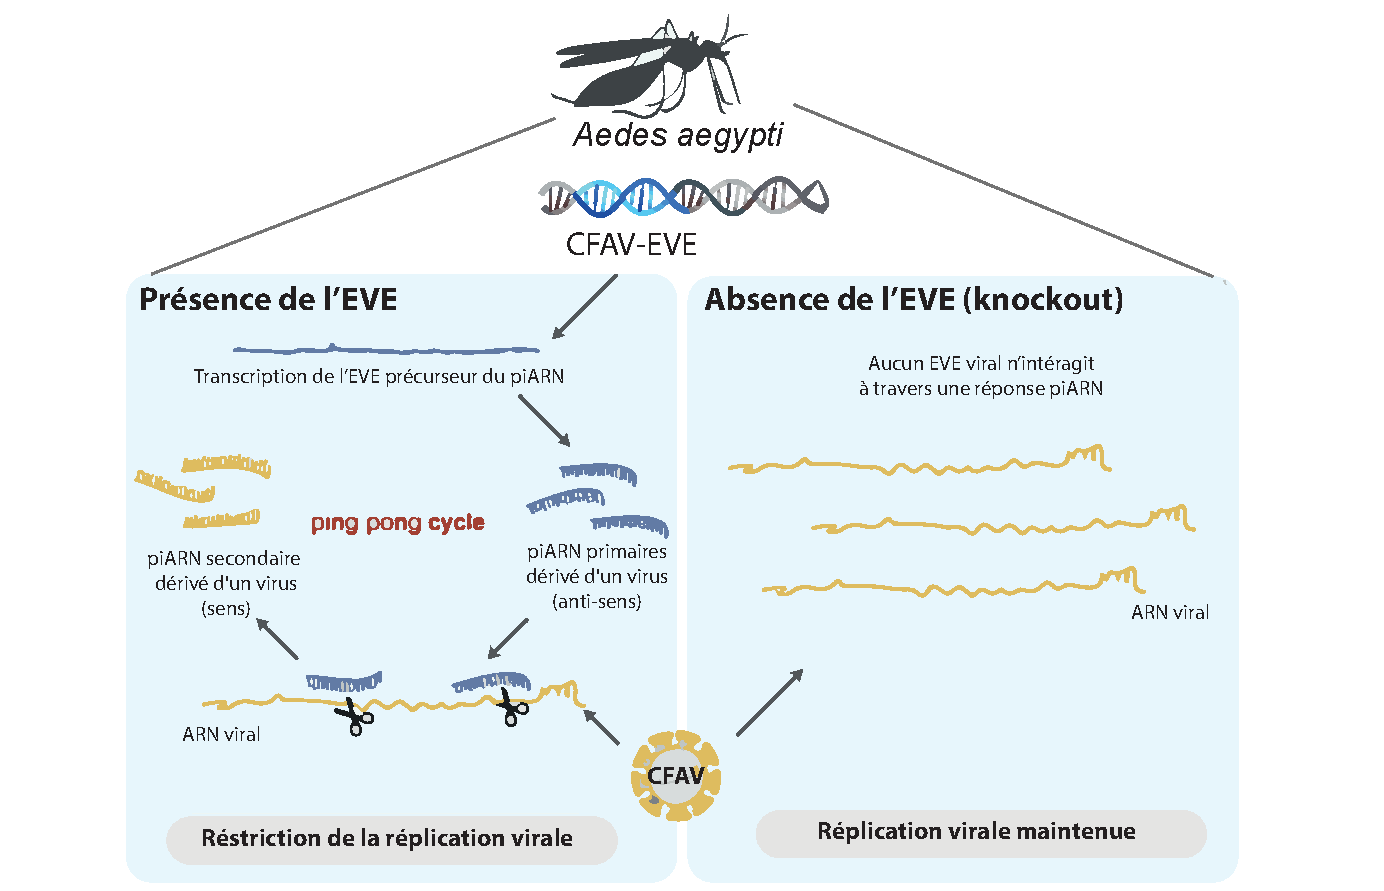
\includegraphics[width=\linewidth,height=\textheight,keepaspectratio]{PhD-master/figures/Antiviral_immunity.pdf}
\caption[Intro:Illustration d'un gène d'arbovirus impliqué dans l'immunité antivirale chez le moustique]{\textbf{Illustration d'un gène d'arbovirus impliqué dans l'immunité antivirale modifié de \cite{suzuki_non-retroviral_2020}}. La recherche systématique d'EVEs dans le génome des moustiques du genre \textit{Aedes} a révélé la présence de nombreuses EVEs au cœur même des clusters de piRNA (régions concentrées du génome produisant les piRNA).Ces clusters sont transcrits à partir des deux brins, et contiennent des centaines à des milliers de gènes de piRNA qui sont souvent organisés en réseaux en tandem. Ainsi, la présence d'EVEs en abondance dans ces régions  soulève la possibilité  que les EVEs participent à une réponse antivirale contre les virus exogènes via la voie des piRNA \citep{palatini_comparative_2017,suzuki_uncovering_2017}. Dans cette fameuse voie, une amplification réciproque des piRNA est effectuée lors d'un cycle ping-pong. Dans ce cycle, les transcrits anti-sens de piRNA précurseur sont produits à partir d'une matrice provenant de l'EVE. Ces transcrits guident le clivage des séquences d'ARN complémentaires qui proviennent d'un virus infectieux suffisamment proche en termes de séquence. S'ensuit le recrutement de complexes protéiques permettant de couper le transcrit viral en plusieurs morceaux. Ces transcrits de piRNA secondaires dérivés du virus induisent ensuite le clivage des transcrits précurseurs de piRNA, transformés ensuite en piRNA primaire, et ainsi de suite, ce qui empêche le virus infectieux de se répliquer correctement.}
\label{figure:Antiviral_immunity}
\end{figure}

\subsection{Réponse à un changement de condition environnementale}

En réponse à des changements environnementaux, certains organismes peuvent modifier leur phénotype, on appelle cela de la plasticité phénotypique. Ce phénomène peut se produire à différents niveaux, du niveau cellulaire au niveau de l'organisme, et même au niveau de la population.

Les pucerons constituent un exemple classique de plasticité phénotypique face à des variations de densité. En cas de surpopulation, certains individus produisent des progénitures ailées. Les pucerons ailés peuvent se disperser dans de nouveaux environnements, mais cela a un coût : ils produisent moins de descendants que leurs homologues dépourvus d'ailes \citep{sutherland_role_1969}. Ainsi, la valeur adaptative d'un individu est déterminée par sa capacité à détecter les conditions environnementales et à y répondre efficacement. 

Chez les clones asexués du puceron rose du pommier (\textit{Dysaphis plantaginea}), la production de la forme ailée est fortement accentuée par l'infection par un densovirus : Dysaphis plantaginea densovirus (DplDNV) \citep{ryabov_densovirus_2009}. En réponse à la surpopulation, dans les conditions expérimentales de l'étude, seuls les clones infectés par le virus ont produit des progénitures ailées, bien qu'ils en aient produit moins que les clones non-infectés \citep{ryabov_densovirus_2009}(\figurename{\ref{figure:Pucerons_densovirus}}-B). 

Ainsi, dans ce système, les virus contribuent à leur propre  dispersion en maximisant la dispersion de leurs hôtes à travers la formation d'individus ailés, mais contribuent peut-être également à la fitness des pucerons en leur permettant de se reproduire sur de nouveaux patchs de ressources. 

De manière remarquable, le puceron du pois (\textit{Acyrthosiphon pisum}, une espèce cousine de \textit{D.plantaginea}) (\figurename{\ref{figure:Pucerons_densovirus}}-A), présente les mêmes phénotypes de dispersion, mais chez ce dernier, c'est la domestication directe de deux gènes de densovirus qui est impliquée dans la plasticité de ce phénotype ailé\citep{parker_laterally_2019} (\figurename{\ref{figure:Pucerons_densovirus}}-C). En effet, à l'intérieur du génome de \textit{A.pisum}, deux gènes fortement exprimés en condition de promiscuité forte, (\textit{Apns-1} et \textit{Apns-2}), ont été découverts. Ces gènes sont en réalité des EVEs dérivant de gènes non structuraux d'un densovirus apparenté à (DplDNV) \citep{parker_laterally_2019}. Ainsi, les génotypes fortement inductibles expriment les gènes \textit{Apns} plus fortement que les génotypes faiblement inductibles, favorisant ainsi la dispersion des pucerons et permettant d'échapper aux conditions de promiscuité (\figurename{\ref{figure:Pucerons_densovirus}}-C).


\begin{figure}[!htpbt]
\captionsetup{font=footnotesize}
 \centering
  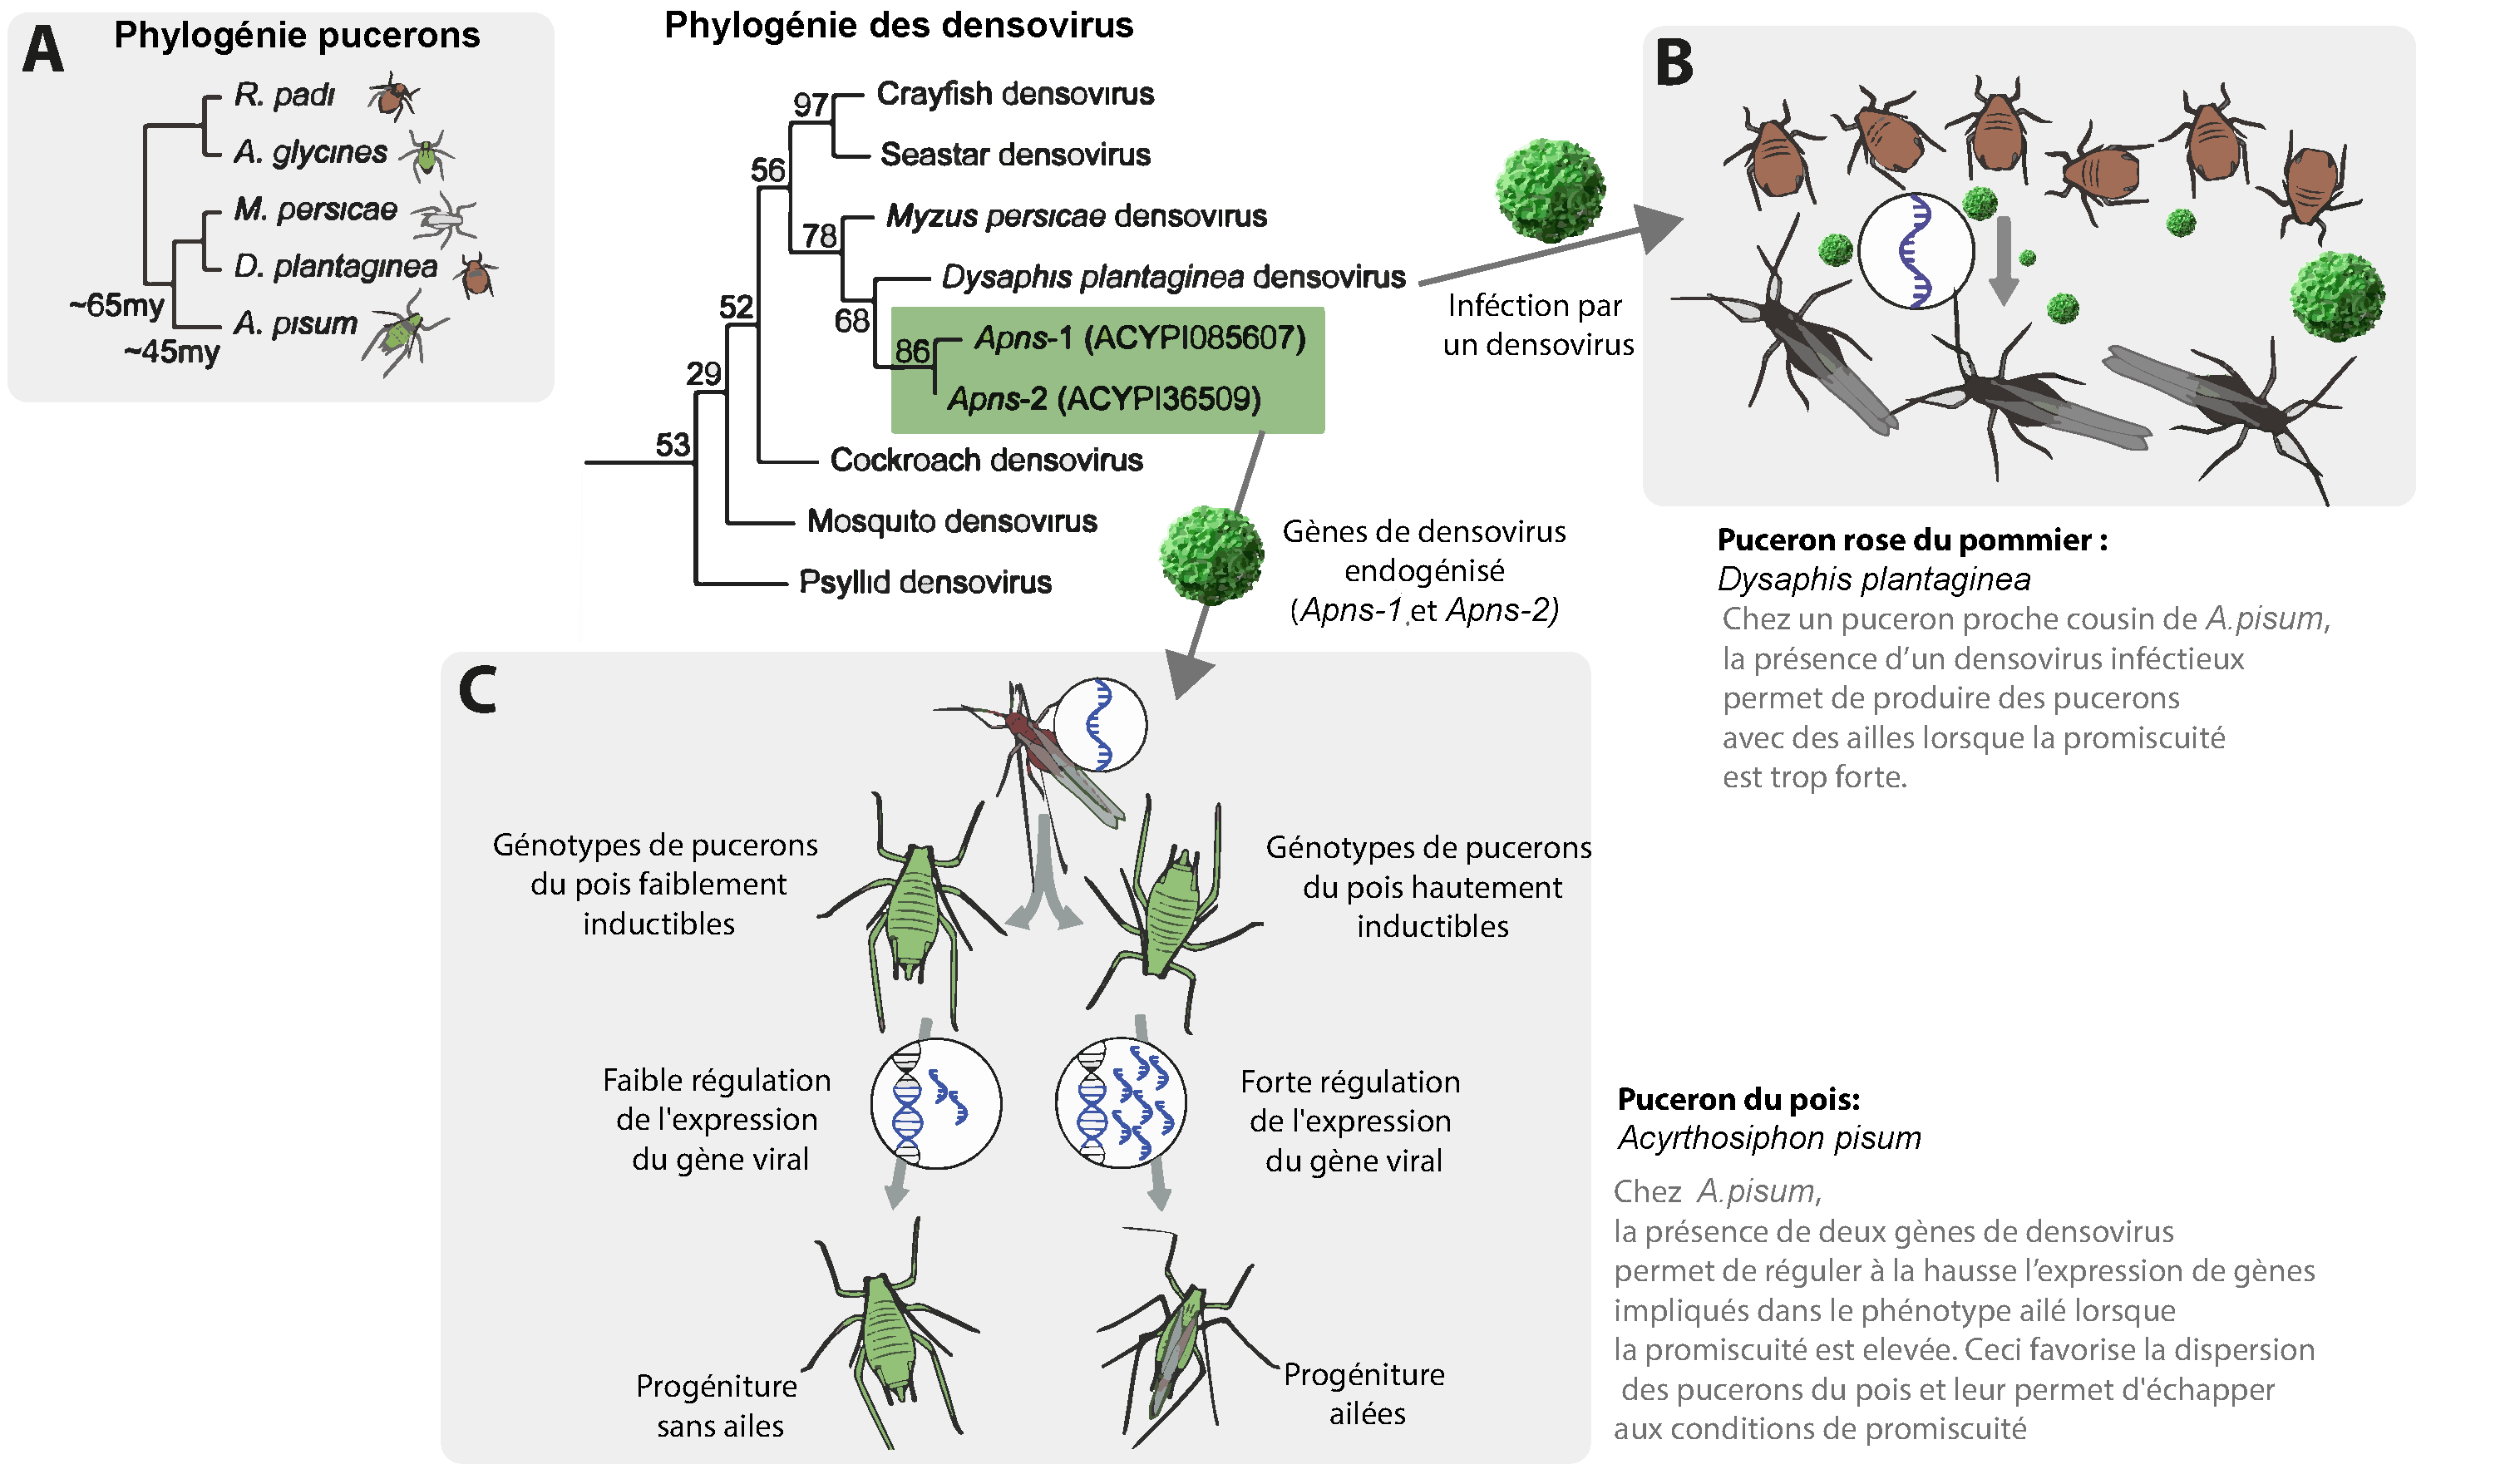
\includegraphics[width=\linewidth,height=\textheight,keepaspectratio]{PhD-master/figures/Pucerons_densovirus.pdf}
\caption[Intro:Illustration d'un gène de densovirus impliqué dans la plasticité phénotypique chez le puceron]{\textbf{Illustration d'un gène de densovirus impliqué dans la plasticité phénotypique modifié de \cite{parker_laterally_2019}}.}
\label{figure:Pucerons_densovirus}
\end{figure}


\subsection{Conclusion sur ces exemples de domestication}

Les évènements de domestication évoqués dans cette partie impliquent en général un nombre restreint de gènes viraux, souvent un seul. Dans la suite, nous allons nous intéresser à d'autres systèmes retrouvés chez des guêpes parasitoïdes. Ces systèmes impliquent la domestication d'une machinerie virale complexe agissant de concert pour produire et assembler des structures virales essentielles au succès reproducteur de ces guêpes. Les particules ainsi produites se nomment des polydnavirus (PDVs) et Virus-like particules (VLPs). À ma connaissance, parmi les organismes eucaryotes, seuls les PDVs et les VLPs domestiqués chez les guêpes parasitoïdes fournissent des exemples de domestication impliquant toute une machinerie virale.

    \chapter{La domestication d'une machinerie virale complexe par des guêpes parasitoïdes}
{\hypersetup{linkcolor=GREYDARK}\minitoc}
\label{chap:intro-parasitoids}

\section{Les Hyménoptères parasitoïdes}

Un parasite désigne un organisme appartenant à une espèce qui profite d’un autre organisme (l'hôte) à ses dépens, parfois sans le tuer (par exemple le parasite de la malaria du genre \textit{Plasmodium}, les poux ou bien le VIH). Un insecte parasitoïde désigne un cas particulier de parasite mélangé à de la prédation puisque les larves se nourrissent à l’intérieur ou sur le corps d’autres arthropodes. Les larves du parasitoïde consomment donc leur hôte. Les guêpes parasitoïdes ont un aspect bien différent des guêpes jaune et noire que l’on connaît bien. Il s’agit plutôt de guêpes de petite taille, pouvant être assez minuscules pour passer à travers le chas d’une aiguille. Les plus grosses ne dépassent que très rarement les quelques cm. La majorité des insectes parasitoïdes est retrouvée au sein de l’ordre des Hyménoptères (dont font partie les guêpes, les abeilles et les fourmis par exemple). Cet ordre est considéré comme le plus diversifié au sein des insectes \citep{forbes_1_2018}, et il est très important sur le plan économique : il contient de nombreuses espèces pollinisatrices ainsi que de nombreuses espèces parasitoïdes qui tuent naturellement d’autres insectes ravageurs de cultures \citep{foottit_biodiversity_2009}. 

Selon une analyse phylogénétique récente, la transition vers le mode de vie parasitoïde s'est produite une seule fois entre le Permien et le Trias il y a 247 millions d'années \citep{peters_evolutionary_2017}, suivi par des épisodes de reversions vers le mode de vie libre, que l'on retrouve aujourd'hui chez les insectes sociaux par exemple. Aussi, la majorité de la diversité des Hyménoptères parasitoïdes se retrouve dans le clade "parasitoida"\citep{peters_evolutionary_2017}(\figurename{\ref{figure:diversite-parasitoid}}- n.7).\\

\begin{figure}[!htpbt]
\captionsetup{font=footnotesize}
 \centering
  \includegraphics[width=\linewidth,height=\textheight,keepaspectratio]{PhD-master/figures/Diversite_parasitoide.pdf}
\caption[Intro:Phylogénie des Hyménoptères]{\textbf{Phylogénie des Hyménoptères modifiée de \cite{peters_evolutionary_2017}}.}
\label{figure:diversite-parasitoid}
\end{figure}

\textbf{Le cycle de vie des guêpes parasitoïdes}

Comme illustré dans la (\figurename{\ref{figure:cycle-de-vie}}), après accouplement, la femelle dépose ses œufs à l’intérieur d’un hôte (on appelle alors ces guêpes des endoparasitoïdes), ou à la surface de l’hôte (on les appelle alors guêpes ectoparasitoïdes). L'hôte est souvent attaqué durant les stades immatures (œufs, larves, pupe) bien que certains parasitoïdes attaquent les adultes. Les œufs puis les larves se développent alors dans ou sur l'insecte hôte jusqu'au dernier stade larvaire, puis chez certaines espèces, les larves sortent de l’hôte pour former une pupe (l’équivalent de la chrysalide chez les papillons), tandis que d'autres forment leur pupe à l'intérieur de l'hôte. Enfin, les adultes émergent de ces pupes, laissant derrière eux dans la grande majorité des cas leur hôte mort. Les espèces hôtes attaqués par ces guêpes sont extrêmement diversifiées. On peut dire que tous les arthropodes à tout stade de vie sont susceptibles d’être parasités par une ou plusieurs espèces de guêpes parasitoïdes \citep{capinera_carabid_2008}. Une guêpe parasitoïde en développement peut, elle-même, être attaquée par un autre parasitoïde, on parle alors d’hyper-parasitoïdisme. 

\begin{figure}[!htpbt]
\captionsetup{font=footnotesize}
 \centering
  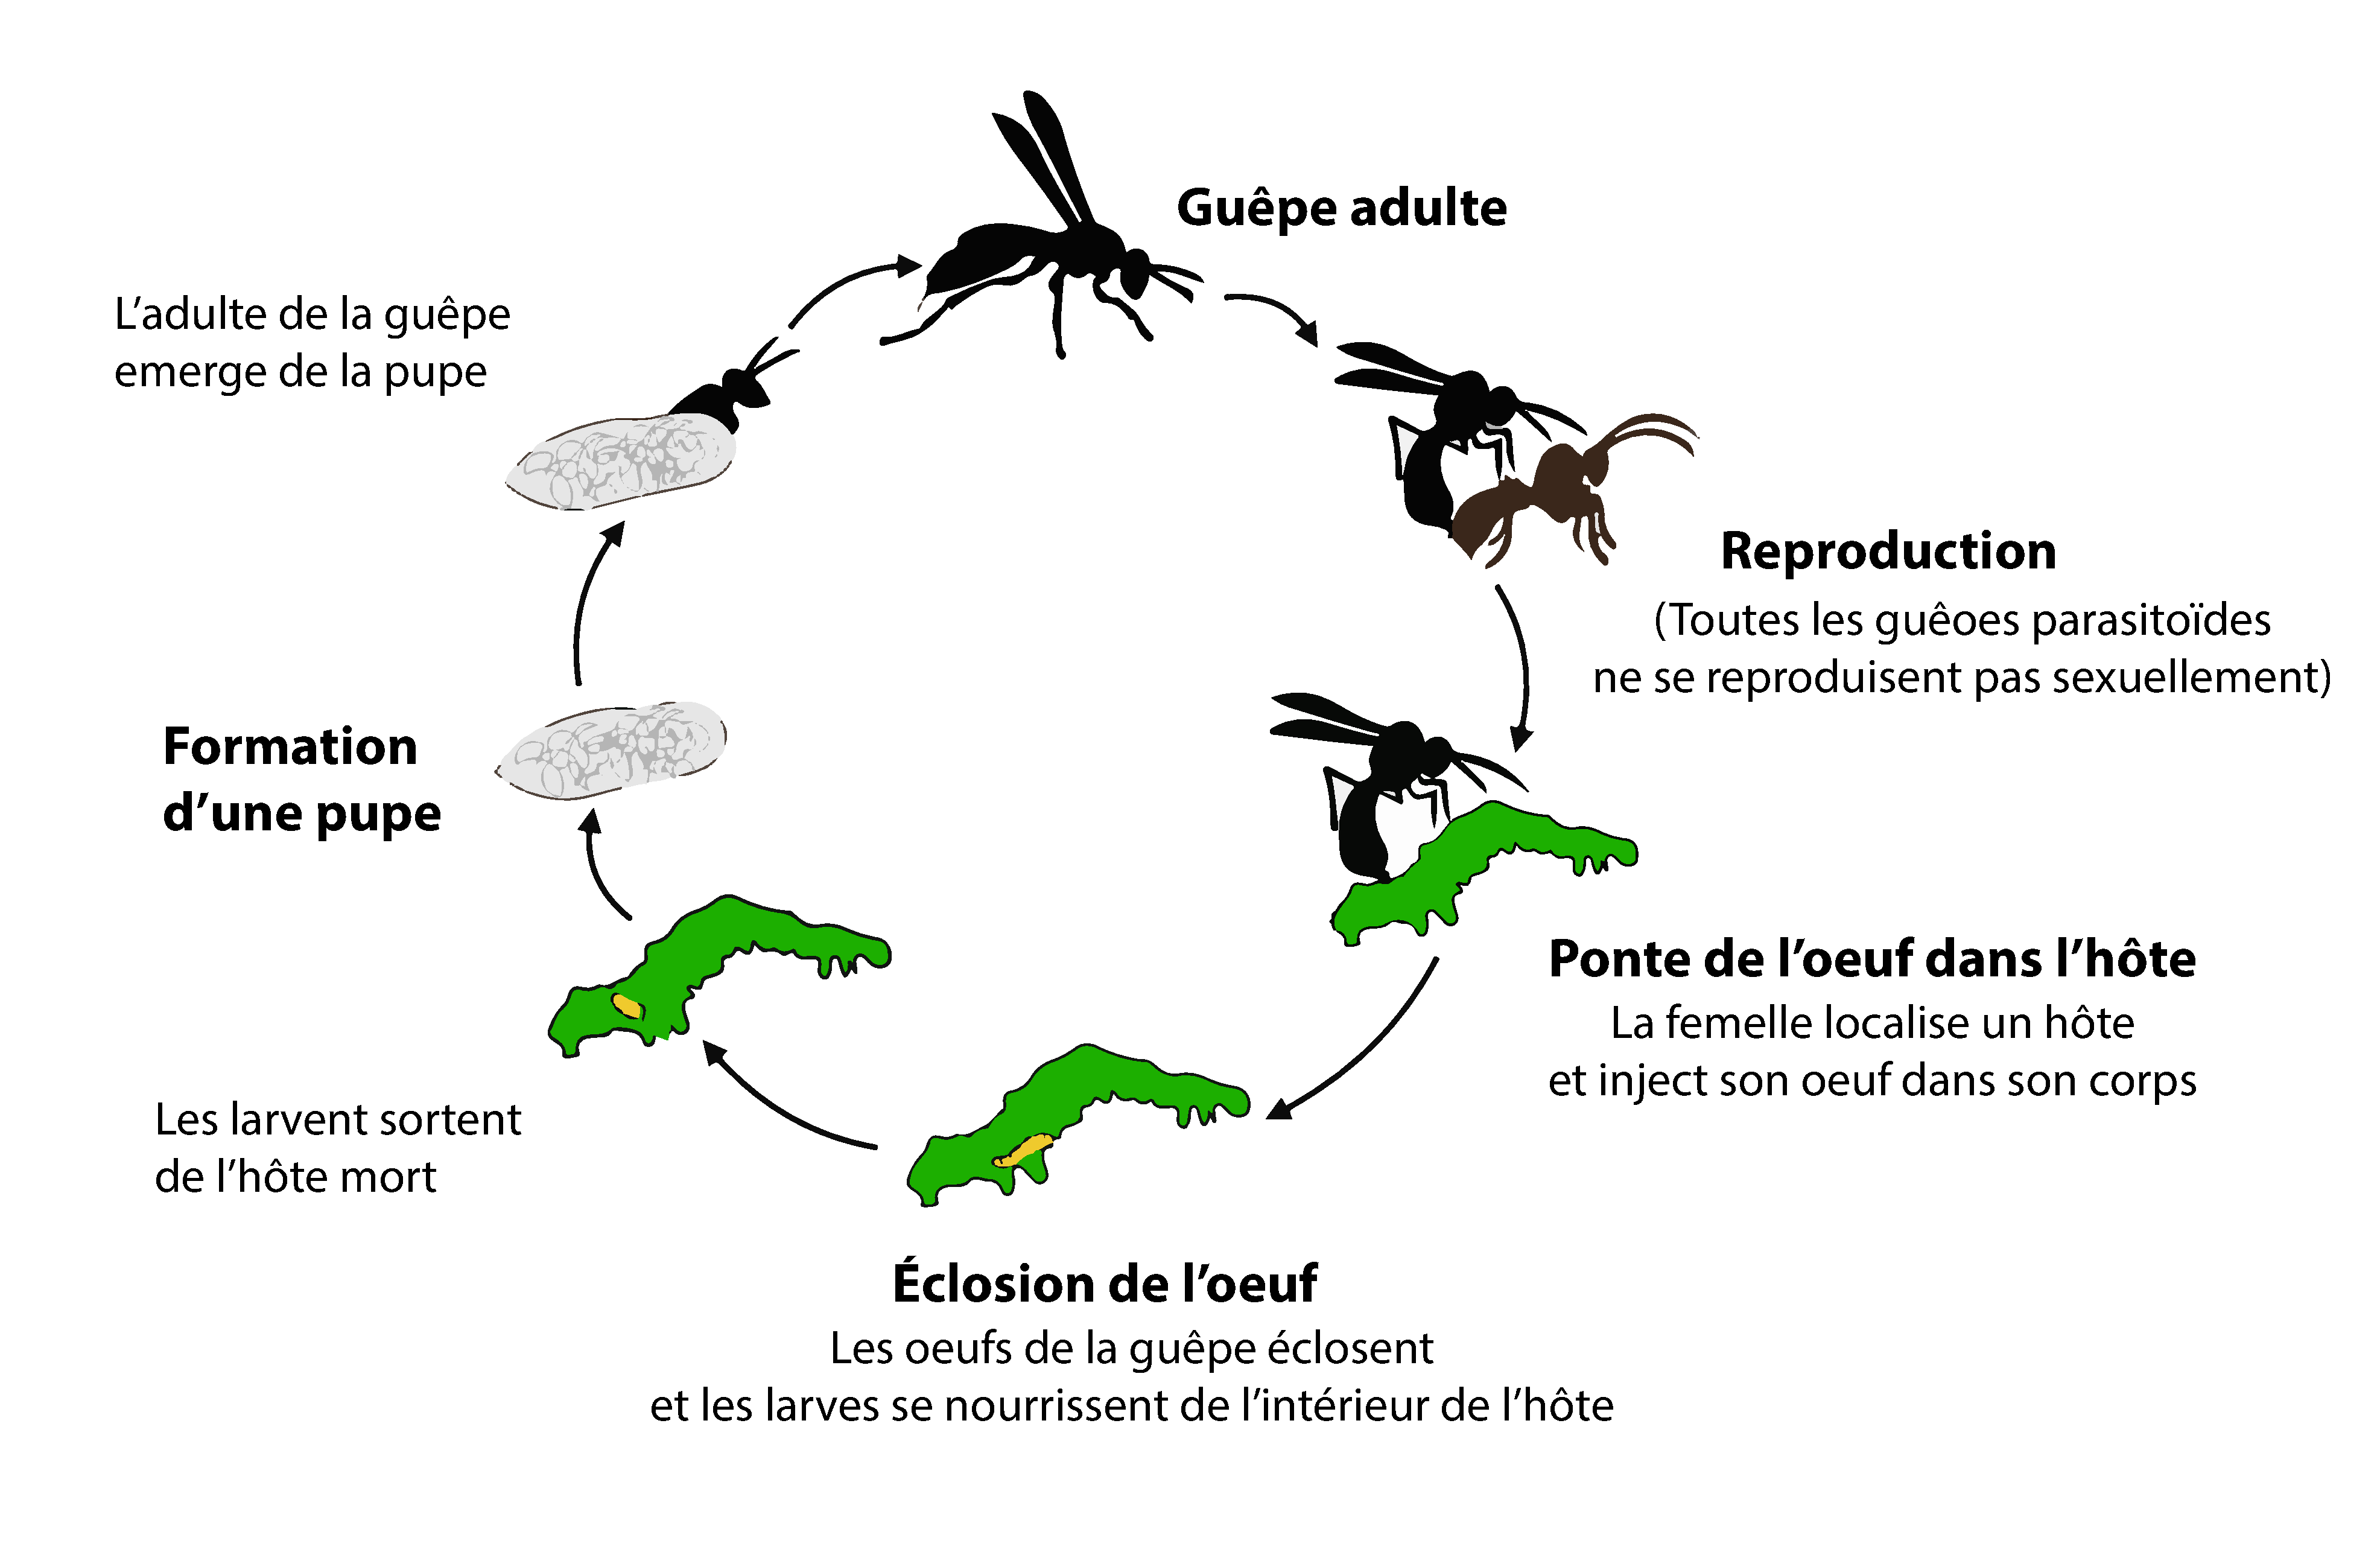
\includegraphics[width=\linewidth,height=\textheight,keepaspectratio]{PhD-master/figures/cycle-de-vie.pdf}
\caption[Intro:Cycle de vie général d'une guêpe endoparasitoïde]{\textbf{Cycle de vie général d'une guêpe endoparasitoïde} modifié de ce \href{https://www.sciencelearn.org.nz/resources/2770-parasitoid-wasp-life-cycle}{site}.}
\label{figure:cycle-de-vie}
\end{figure}

\section{Parasitoïdisme, une lutte incessante du parasitoïde contre son hôte}

Face aux parasitoïdes, les insectes  attaqués réagissent à travers une réponse immunitaire cellulaire. L'une des réponses les plus claires à l'infection par les guêpes est l'encapsulation de l'œuf de guêpe ou de l'embryon précoce. Cette réaction immunitaire innée a été documentée chez de nombreux arthropodes \citep{brehlin_immune_1988}. Par exemple, chez \textit{D.melanogaster}, l'injection d'un œuf de parasitoïde déclenche la production de davantage de plasmatocytes, de lamellocytes et une activation de la cascade de la phénoloxydase (PO) \citep{kim-jo_drosophila_2019}. Les plasmatocytes vont alors former une première couche de cellules autour de l'œuf de parasitoïde à laquelle les lamellocytes adhérent, formant ainsi des jonctions serrées pour former une capsule multicouche mélanisée. La cascade de PO produit ensuite des radicaux cytotoxiques, ce qui entraine la mort de l'œuf du parasitoïde \citep{kim-jo_drosophila_2019} (\figurename{\ref{figure:Encapsulation_process}}). 

\begin{figure}[!htpbt]
\captionsetup{font=footnotesize}
 \centering
  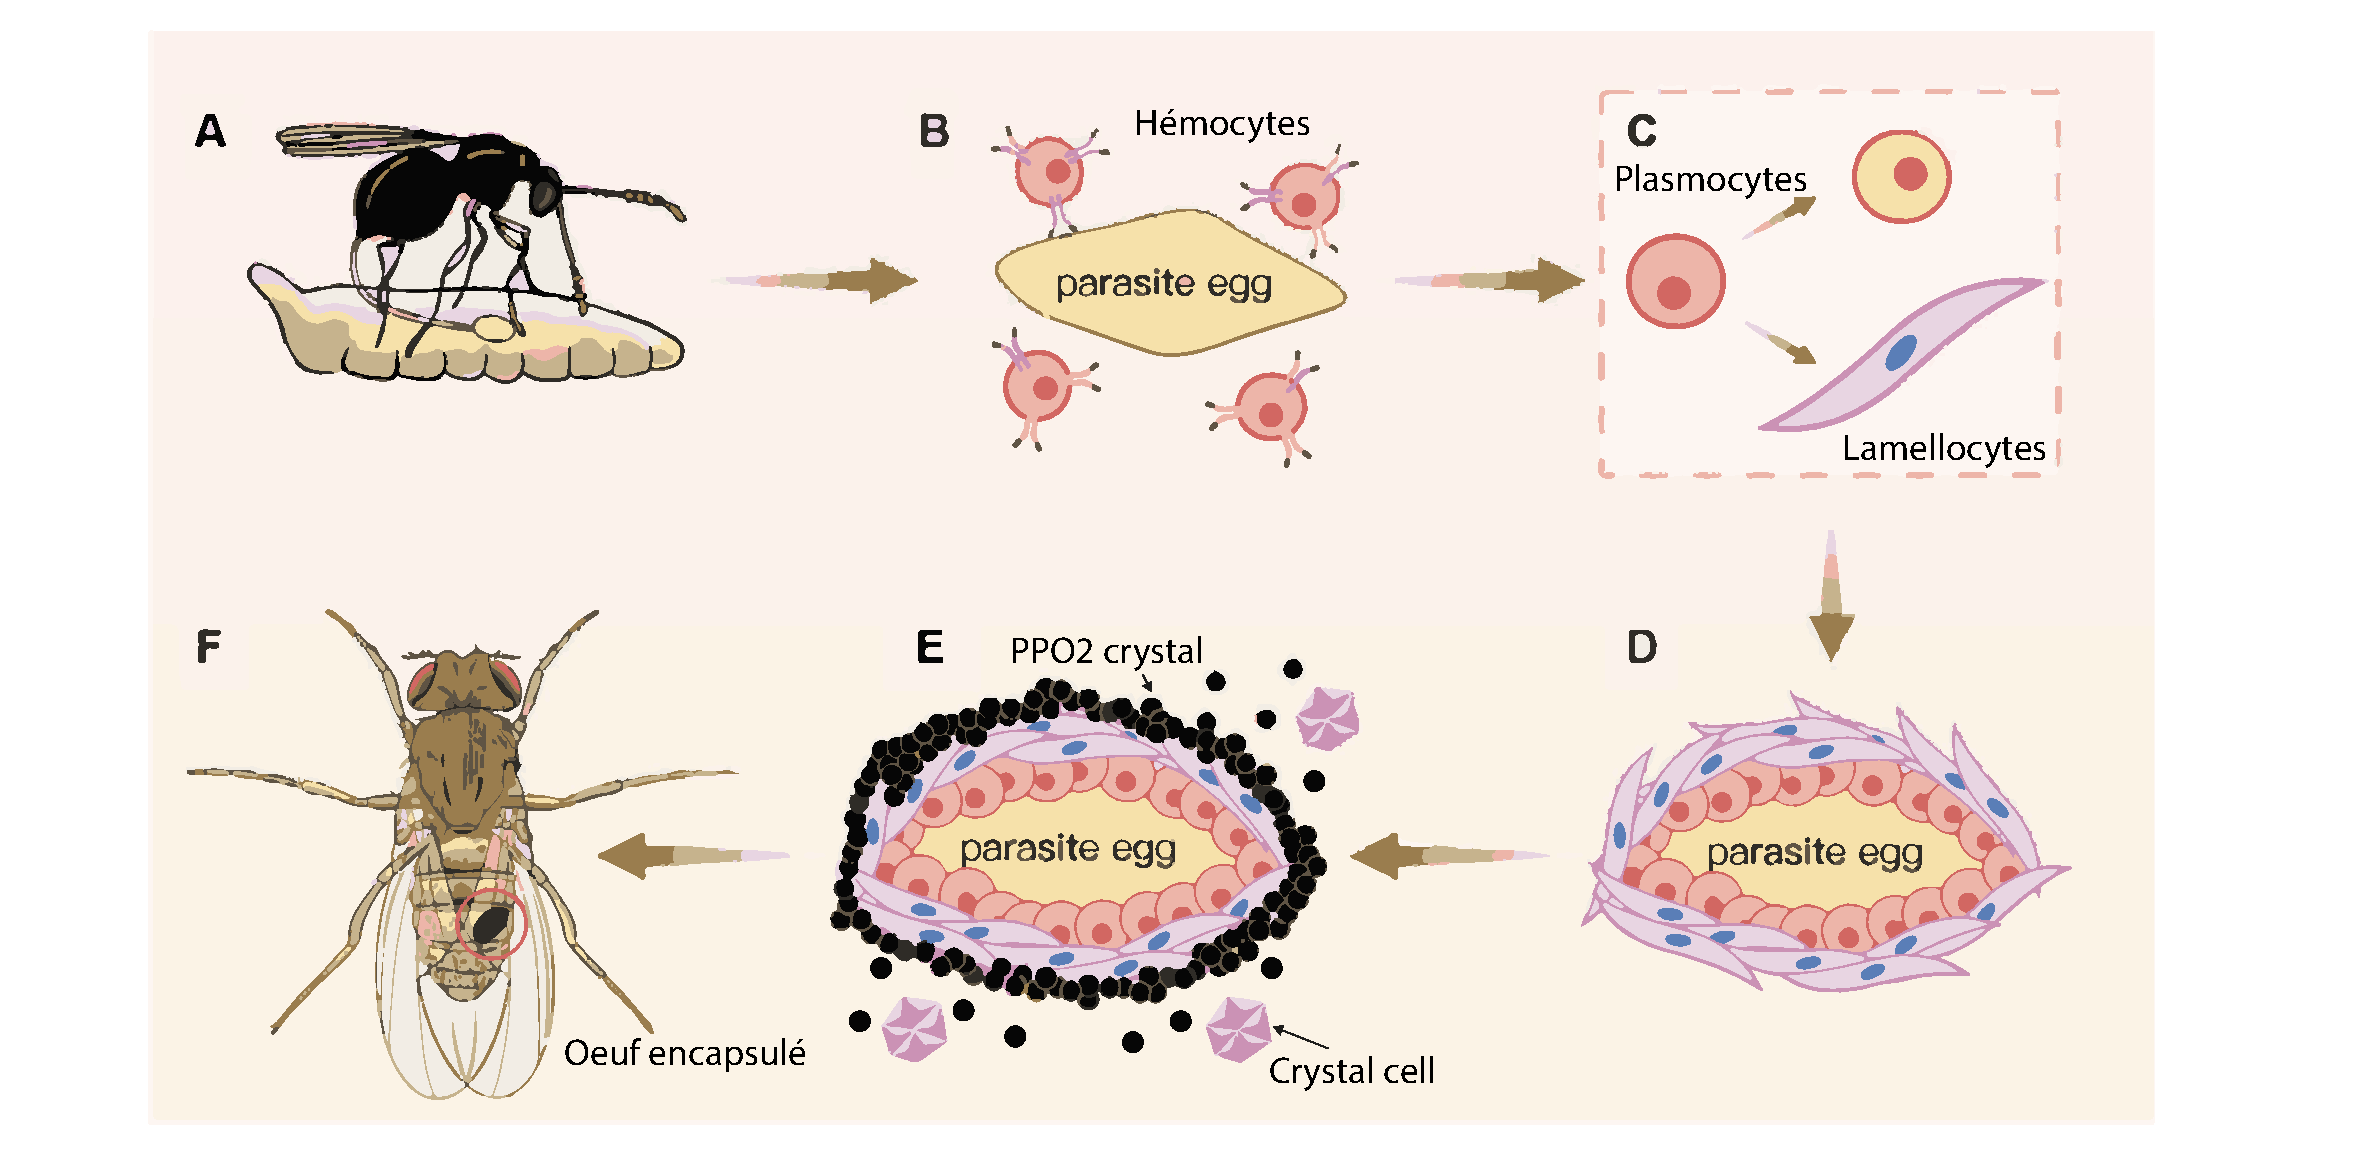
\includegraphics[width=\linewidth,height=\textheight,keepaspectratio]{PhD-master/figures/Encapsulation_process.pdf}
\caption[Intro:Schéma d'encapsulation général chez la drosophile]{\textbf{Les réponses de défense immunitaire de la drosophile hôte à l'encapsulation des œufs de guêpe tiré de \cite{yang_cellular_2021}}. \textbf{A} - La guêpe pond ses œufs dans l'hémocoele de l'hôte. \textbf{B} - Reconnaissance du non-soi médiée par les hémocytes sur les œufs de guêpe.\textbf{C} - Le recrutement des hémocytes implique la prolifération des plasmatocytes et la différenciation des lamellocytes. \textbf{D} - Les plasmatocytes et les lamellocytes migrent vers les œufs et les isolent. La formation de la mélanisation entourant les œufs de guêpe. \textbf{F} -  La guêpe périt, tandis que la drosophile survit.}
\label{figure:Encapsulation_process}
\end{figure}


Face à ce parasitoïdisme, il existe une asymétrie entre les deux entités puisque le parasitoïde est exposé à chaque génération au système immunitaire de son hôte. À l'inverse, la probabilité pour l'hôte d'être parasitoïdé varie fortement dans le temps ou l'espace \citep{fleury_chapter_2009}. Ainsi, du côté des parasitoïdes, de fortes pressions de sélection s'exercent sur leur capacité à contourner l'immunité et à modifier la physiologie de leur hôte (deux caractéristiques clés impliquées dans leur succès reproducteur). Diverses stratégies de contournement du système immunitaire ont donc été sélectionnées au cours de l'évolution. 

La forme de défense active la plus courante est l’injection de toxines (venin) par la femelle parasitoïde dans l'hémolymphe de l'hôte pendant la ponte \citep{asgari_venom_2011, moreau_venom_2015}. Ces toxines ont alors pour fonction d'inhiber le système immunitaire de l’hôte ou d'interrompre son développement \citep{moreau_venom_2015}. 

En termes d'interactions, alors que les guêpes ectoparasitoïdes utilisent leur venin pour conserver la nourriture pour leurs progénitures via la paralysie, les guêpes endoparasitoïdes utilisent leur venin pour transformer les hôtes pour que leurs progénitures puissent vivre et se nourrir jusqu'à l'éclosion \citep{moreau_chapter_2009,schendel_diversity_2019}. De plus, plusieurs études montrent que les espèces ectoparasitoïdes interagissent moins avec le système immunitaire de leurs hôtes comparé à des espèces au style de vie endoparasitoïde qui sont elles complétement plongée dans le corps de leurs hôtes, là où se trouvent notamment toutes les cellules de l'immunité \citep{li_parasitism_2018}. Chez les endoparasitoïdes, sauf dans quelques cas où une paralysie transitoire a été observée, le venin n'a généralement pas d'effet paralysant sur l'hôte, mais a  plutôt un effet de répression du système immunitaire. Après l'endoparasitoïdisme, l'hôte se rétablit généralement en quelques minutes et jusqu'à une heure. Les endoparasitoïdes évitent d'induire une paralysie à long terme chez l'hôte et adoptent un mode de vie dit koïnobionte. Dans ce cas, l'hôte est maintenu en vie et poursuit son développement, le parasitoïde étant toujours à l'intérieur \citep{moreau_venom_2015}.\\

Dans de nombreux systèmes parasitoïde-hôte, l'injection de substances particulières au sein de ces venins maternels permet également d'assurer le succès du parasitoïde. L'origine de ces substances a longtemps été débattue dans la communauté scientifique et nous savons aujourd'hui qu'une partie provient de la domestication de virus chez certaines espèces de guêpes endoparasitoïdes. Afin d'illustrer ce cas particulier, je vous propose une courte rétrospective historique pour résumer cette découverte (inspirée de l'ouvrage \textit{Parasitoid Viruses : Symbionts and Pathogenes} \citep{strand_polydnavirus_2012}).\\

Les racines de la découverte que je m'apprête à exposer proviennent du chercheur britannique George Salt qui, en 1965, montre que les fluides produits dans le calice (organe situé à la base des ovaires chez certains parasitoïdes comme ici chez le braconidae \textit{Venturia canescens}) protègent les œufs de l’encapsulation. Étrangement, en 1967, Susan Rotheram observe chez la même espèce, que de nombreuses « particules » produites dans les cellules du calice s'accrochent aux œufs \citep{rotheram_immune_1967,noauthor_surface_1973}. Pour certains.es observateurs·rices de l’époque, il s'agissait de virus compte tenu de leurs structures et de leurs tailles. Plus tard, chez une autre espèce de Braconidae (\textit{Cardiochiles nigriceps}), un traitement à la DNAse permet de mettre en évidence la présence d'ADN à l'intérieur des particules observées \citep{vinson_particles_1975}. Par la suite, des analyses complémentaires chez plusieurs genres de parasitoïdes issues de la superfamille des Ichneumonoidea (\textit{Toxoneuron}, \textit{Microplitis}, \textit{Chelonus} et \textit{Campoletis}) montrent des différences morphologiques notables entre les particules observées selon les espèces. La littérature jusqu'au début des années 1990 a donc majoritairement conclu que les particules observées étaient des virus, car ils : 1) se répliquent dans les cellules du calice des guêpes, 2) ressemblent morphologiquement à des virus, 3) contiennent des acides nucléiques, 4) sont infectieux, et 5) contiennent des gènes qui sont transcrits après l'infection des hôtes \citep{fleming_polydnaviruses_1992,stoltz_viruses_1979}. C’est à ce moment-là que le nom de « virus-like », puis polydnavirus (PDVs) (car les particules sont composées de plusieurs molécules d'ADN) a été proposé pour décrire ces particules virales ayant l'apparence de virus. Par la suite, en 1984, l'établissement d’une nouvelle famille virale est proposé et validé par la communauté scientifique (les \textit{Polydnaviridae}) \citep{stoltz_polydnaviridae_1984}. C’est en 2004 que le premier génome de polydnavirus est séquencé chez le Braconidae \textit{Cotesia congregata}. Cette découverte va chambouler la vision des chercheurs.euses de l’époque. Étonnamment, à l’intérieur de ces particules, aucun ADN apparenté à des virus connu n'est retrouvé. À l'inverse, les cercles d'ADN codent très majoritairement des facteurs de virulence d'origine eucaryote \citep{espagne_genome_2004,desjardins_comparative_2008}. Le séquençage des particules révèle donc que les gènes essentiels à leur production ne sont pas contenus dans les particules. C’est ainsi qu’en 2009, \cite{bezier_polydnaviruses_2009} identifient et confirment, grâce à l'étude du transcriptomique et du protéome de \textit{Cotesia congregata} pendant la phase de production des particules, la présence d'un ensemble de gènes d'origine virale impliqués dans la production de ces particules. Ce virus endogène est par la suite baptisé bracovirus du nom de la famille d’Hyménoptère Braconidae chez qui ces séquences ont été décrites pour la première fois. 
Il devient alors assez clair que les PDVs sont incapables de se répliquer dans l'hôte comme le font tous les virus, mais font plutôt partie intégrante du génome des guêpes.\\

\section{Biologie des structures virales délivrant des facteurs de virulence}

Depuis 2009, de nombreuses études ont précisé notre compréhension de l'histoire de l'acquisition et de l'utilisation de ces particules virales chez les guêpes apparentées à \textit{Cotesia congregata}. Nous savons aujourd'hui que ces particules virales sont codées par des gènes provenant d'un virus ancien qui a été endogénisé chez l'ancêtre commun de plusieurs milliers d'espèces appartenant au complexe des microgastroïdes \citep{strand_polydnaviruses_2015}. 

Ces « virus » ou plutôt gènes viraux domestiqués sont transmis verticalement via les chromosomes de la guêpe \citep{bezier_polydnaviruses_2009}. Ces gènes ne suivent en revanche pas les différentes étapes d'un cycle de vie viral, qui consiste à infecter des cellules cibles et à produire une descendance en créant de nouvelles particules. En effet, ce virus n'est plus libre à proprement parler, car les gènes viraux impliqués dans la synthèse des "virus" sont présents en permanence dans le génome de la guêpe. De plus, l'ADN codant pour les protéines induisant la réplication, l'empaquetage et l'enveloppement des virions n'est pas présent dans les particules infectieuses : ces virus ne sont donc plus infectieux \citep{strand_polydnaviruses_2015}. En ce sens, ces particules ne sont pas des virus typiques ; il s'agit plutôt d'entités hybrides "mi-virus mi-guêpe". 

Les particules virales ainsi produites servent de véhicules à la guêpe pour délivrer des composants spécifiques (que nous appellerons "facteur de virulence") directement aux cellules du système immunitaire de l'hôte. Ces facteurs de virulence sous forme de cercles d'ADNs sont alors adressés aux cellules immunitaires, puis s'intègrent dans les chromosomes de la cellule pour être exprimés par la machinerie cellulaire de l'hôte. Ces facteurs sont cruciaux pour le succès parasitaire, car ils comprennent différents éléments qui modifient la physiologie de l'hôte, rendant ce dernier plus adapté au développement des progénitures de guêpes \citep{gauthier_recurrent_2018}. 

Les facteurs de virulences se trouvent sous forme de gènes dans des cercles d'ADN double brin produits par les guêpes. Ces gènes sont pour la plupart d'origine de la guêpe (e.g. lectines de type C, protéine tyrosine phosphatase (ptp), ankyrines (ank), Egf) \citep{desjardins_comparative_2008, gasmi_recurrent_2015,huguet_evolution_2012}, tandis que d'autres plus rares dérivent d'éléments transposables (TE) \citep{zhang_chromosome-level_2019, gauthier_chromosomal_2021}. La quantité et la nature des gènes présents dans les cercles varient considérablement entre les espèces de guêpes, ce qui s'explique probablement par des phénomènes d'adaptation à différents hôtes \citep{bezier_functional_2013,serbielle_evolutionary_2012, strand_polydnaviruses_2012,cerqueira_de_araujo_chelonus_2022,mao_complete_2022}.
Par exemple, le contenu génique des bracovirus des guêpes parasitoïdes des familles Microgastrinae, qui pondent leurs œufs au stade larvaire, est différent de celui du parasitoïde \textit{Chelonus inanitus} (Cheloninae) qui parasite son hôte au stade œuf \citep{weber_transcriptional_2007, mao_complete_2022, cerqueira_de_araujo_chelonus_2022}. 

Ces cercles qui renferment ces facteurs de virulence proviennent des segments proviraux le long du génome des guêpes. Les segments proviraux appartiennent à des unités qui sont amplifiées pendant la formation des particules dans les cellules du calice \citep{louis_bracovirus_2013, burke_microplitis_2015}. Parmi ces unités amplifiables (unités de réplication), certains segments sont excisés et circularisés par recombinaison spécifique, ce qui nécessite des jonctions de répétition directe (DRJ) à leurs extrémités \citep{beck_encapsidated_2011,desjardins_structure_2007}(\figurename{\ref{figure:polydnavirus_integration_mechanism}}).

Une fois formés, les cercles d'ADN sont empaquetés dans des particules virales qui s'accumulent dans le calice, puis sont injectées dans l'hôte avec les œufs pendant l'oviposition \citep{strand_polydnaviruses_2014}. Ces particules s'attachent ensuite aux cellules de l'immunité pour y libérer les cercles d'ADN.  Dans le cas de certains polydnavirus étudiés, la majorité des cellules cibles sont des cellules immunitaires, comme les hémocytes \citep{beck_novel_2007}, mais ces particules peuvent également pénétrer dans presque tous les tissus, y compris les cellules de l'intestin et les cellules nerveuses \citep{beck_novel_2007, muller_genome-wide_2021}. Quoi qu'il en soit, parmi ces cercles, la majorité vont s'intégrer dans les chromosomes des cellules immunitaires \citep{chevignon_cotesia_2018, muller_genome-wide_2021} où les facteurs de virulence codés s'y trouvent exprimés \citep{pruijssers_ptp-h2_2007} permettant \textit{in fine} d’éviter la réponse immunitaire de l’insecte hôte \citep{drezen_endogenous_2017}.

Les mécanismes d'intégration de ces cercles viraux à l'intérieur du génome de l'hôte commencent à être bien décrits. Elle se produit grâce à un motif porté par certains cercles appelé motif d'intégration de l'hôte (HIM)\citep{beck_encapsidated_2011,chevignon_cotesia_2018,muller_genome-wide_2021}. Les intégrations de ces cercles impliquent deux jonctions, appelées jonction 1 (J1) et jonction 2 (J2), situées dans le HIM. Ces motifs sont par ailleurs conservés entre les espèces \textit{C.vestalis} et \textit{C.vestalis}\citep{mao_complete_2022}. J1 et J2 correspondent aux séquences qui forment les extrémités des séquences virales lorsqu'elles sont intégrées dans l'ADN de l'hôte (\figurename{\ref{figure:polydnavirus_integration_mechanism}}).

\begin{figure}[H]
\captionsetup{font=footnotesize}
 \centering
  \includegraphics[width=\linewidth,height=\textheight,keepaspectratio]{PhD-master/figures/polydnavirus_integration_mechanism.pdf}
\caption[Intro:Mécanisme d'intégration des cercles d'ADN]{\textbf{Mécanisme d'intégration des cercles d'ADN}. Les cercles d'ADN proviennent de séquences provirales contenues dans le génome de la guêpe. Ces segments proviraux contiennent des facteurs de virulence (loci rouges). Après amplification des segments proviraux, les molécules d'ADN produites sont circularisées par un mécanisme de recombinaison spécifique au site impliquant des répétitions directes légèrement différentes correspondant aux extrémités des segments proviraux (jonctions de répétition directe 5' (DRJ) et jonctions de répétition directe 3' (DRJ) : jaune et orange). La séquence circulaire comprend une DRJ circulaire (ou motif de jonction circulaire), une forme recombinée distincte des DRJ 5' et 3' (locus jaune/orange). De plus, les cercles d'ADN peuvent s'intégrer dans l'ADN génomique de l'hôte par un mécanisme impliquant très probablement une intégrase puis médié par des motifs d'intégration de l'hôte (HIM), indiqués par des lignes bleues. Une fois intégrés dans le génome, les facteurs de virulence vont être transcrits par la cellule hôte, et vont altérer la physiologie de la cellule, ce qui va l'empêcher de remplir sa fonction immunitaire.}
\label{figure:polydnavirus_integration_mechanism}
\end{figure}

De manière remarquable, d'autres espèces de guêpes parasitoïdes ont également domestiqué des virus de manière complètement indépendante. Dans tous les cas, ces virus domestiqués remplissent la même fonction biologique, c'est-à-dire qu'ils permettent de désactiver efficacement le système immunitaire de l'hôte.  Ainsi, selon l'espèce de guêpe, ces structures produites peuvent renfermer des facteurs de virulence sous forme de cercles d'ADN codant pour les gènes de virulence (chez les espèces connues pour produire des polydnavirus comme décrit plus haut, PDV)(\figurename{\ref{figure:PDV_VLP}}), ou sous forme de protéines (chez les espèces connues pour produire des protéines de type virales, VLP)(\figurename{\ref{figure:PDV_VLP}}). 

La propriété principale ayant été recrutée à plusieurs reprises, que ce soit chez les PDVs ou les VLPs est donc la capacité de fusionner les membranes (à l'image des \textit{syncitins} ou bien des gènes \textit{arc}) pour pénétrer à l'intérieur des cellules immunitaires de l'hôte. 

Dans les deux types de structures, toutes les fonctions majeures de l'ancêtre des virus domestiqués (excepté une réplication de l'ADN) ont été conservées : la transcription virale, l'empaquetage et l'infectivité \citep{drezen_endogenous_2017}. Les gènes impliqués dans la transcription virale au cours d'un processus infectieux, tels que les sous-unités de l'ARN polymérase virale (\textit{lef-4}, \textit{lef-8}, \textit{lef-9} et \textit{p47}), sont exprimés au début du développement nymphal de la guêpe et sont supposés réguler l'expression d'autres gènes viraux, tels que ceux codant pour les composants des nucléocapsides et des protéines d'enveloppe (\figurename{\ref{figure:PDV_VLP}}). 

\begin{figure}[H]
\captionsetup{font=footnotesize}
 \centering
  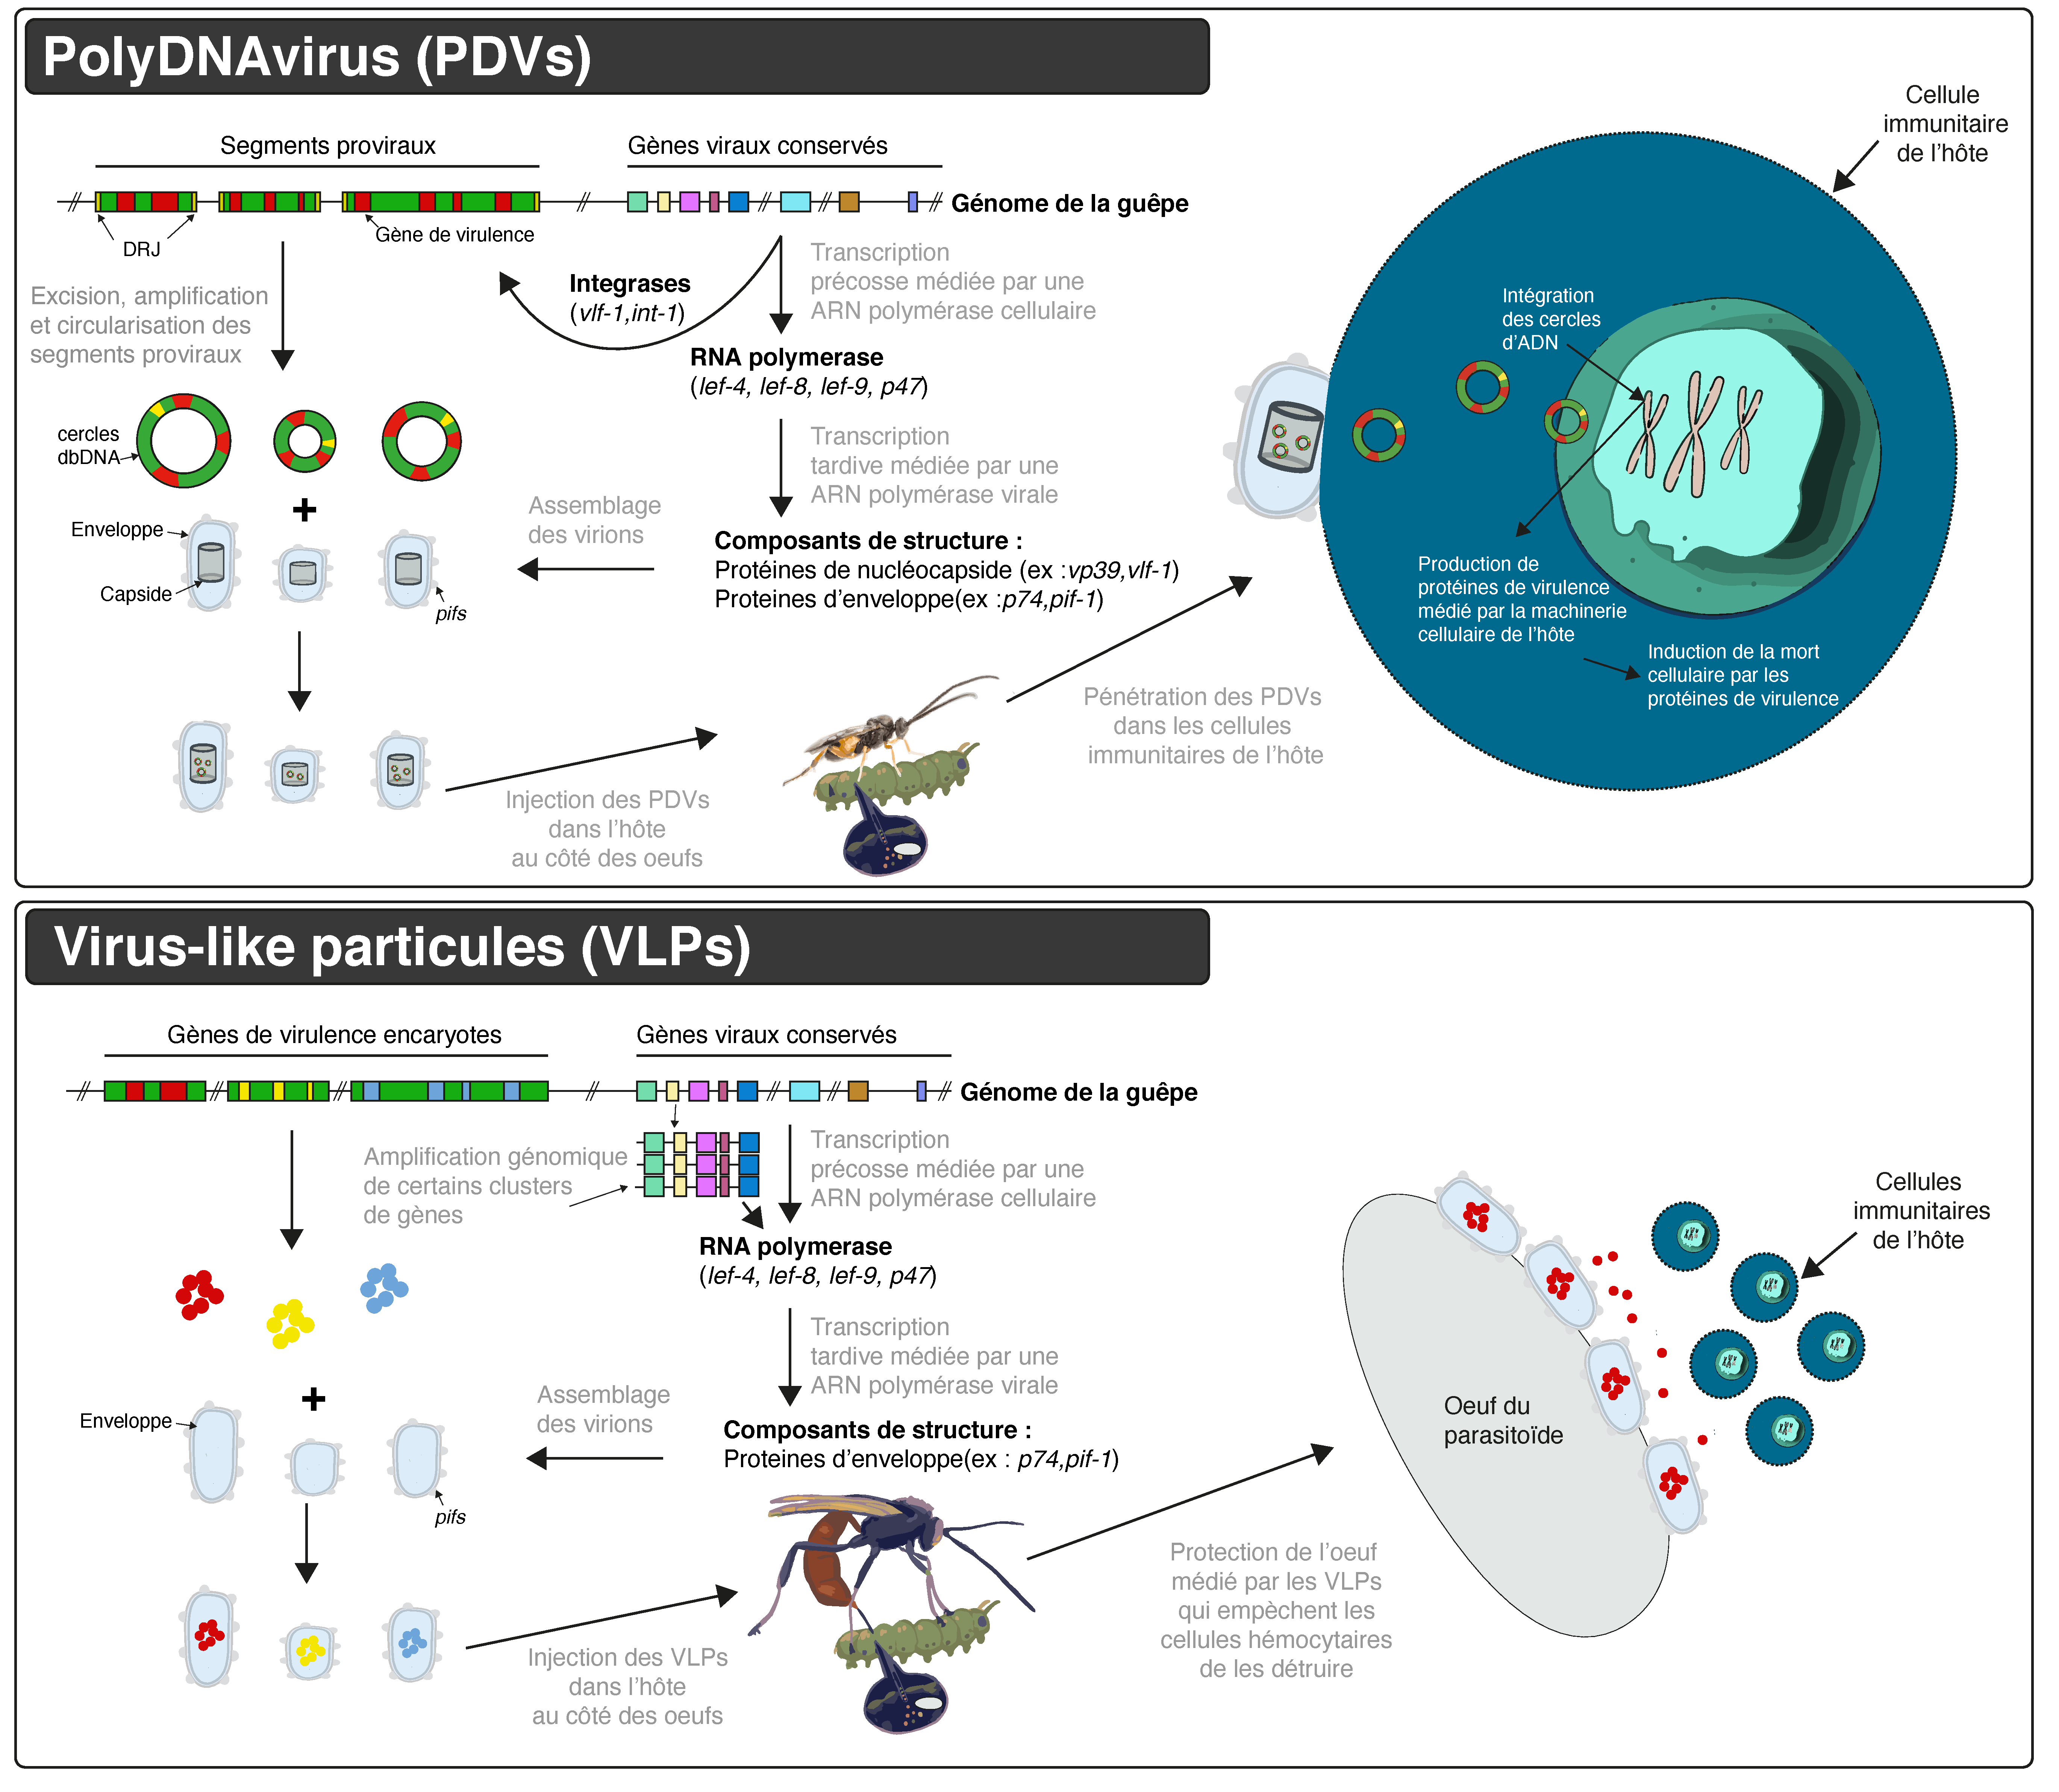
\includegraphics[width=\linewidth,height=\textheight,keepaspectratio]{PhD-master/figures/PDV_VLP.pdf}
\caption[Intro:Différentes structures à allures virales produites par les guêpes parasitoïdes]{\textbf{Différentes structures à allures virales produites par les guêpes parasitoïdes} }
\label{figure:PDV_VLP}
\end{figure}


\section{Les différents cas de domestications virales  chez les guêpes parasitoïdes}

Finalement, jusqu'à présent, six cas indépendants d'événements de domestication virale ont été rapportés, tous impliquant des donneurs de virus à ADN double brins de l'ordre des \textit{Lefavirales}. La plupart de ces événements de domestication se trouvent dans la super-famille des Ichneumonoidea, où 5 cas indépendants d'endogénisation virale sont décrits (\figurename{\ref{figure:Virus_arthropods_phylogeny}}-B). Le mieux documenté concerne l'intégration d'un génome nudiviral (grand virus à ADN double brin) il y a environ 100 millions d'années au sein du complexe des Microgastroïdes (Braconidea) qui contient des milliers d'espèces (on appelle les particules virales produites des bracovirus) (1) \citep{bezier_polydnaviruses_2009,whitfield_systematics_2018} (\figurename{\ref{figure:Virus_arthropods_phylogeny}}-B). Un autre exemple de polydnavirus implique 2 événements indépendants au sein des Ichneumonidea des sous-familles Banchinae (2) et Campopleginae (3) (on appelle les particules virales produites des ichnovirus) \citep{volkoff_analysis_2010,beliveau_genomic_2015}. Dans ce cas, les gènes qui permettent la production des particules virales contenant des cercles d'ADN sont regroupés dans des régions du génome de la guêpe (appelées IVSPERs) qui sont amplifiées lors de la réplication des particules virales, mais qui ne sont pas emballées dans les particules. Ces gènes ne présentent néanmoins pour l'heure aucune homologie de séquence dans les bases de données virales \citep{volkoff_analysis_2010}. Enfin, plus récemment, des cas de domestication de virus impliquant la production de VLPs ont été décrits chez l'espèce \textit{Venturia canescens} (bien qu'il s'agisse de l'espèce ou tout a commencé avec Rotheram et Salt) (4) \citep{pichon_recurrent_2015} et l'espèce \textit{Fopius arisanus} au sein de la sous-famille Opiinae (5) \citep{burke_rapid_2018}. \\

Bien que la super-famille des Ichneumonoidea soit la plus diverse des Hyménoptères \citep{klopfstein_darwin_2019,shimizu_integrative_2020}, elle ne représente qu'une petite partie de la diversité des Hyménoptères parasitoïdes \citep{forbes_1_2018} (\figurename{\ref{figure:diversite-parasitoid}}-B). D'autres espèces plus éloignées sont également concernées par ces phénomènes. En effet, nous avons récemment observé au sein du laboratoire que les VLPs produites par des guêpes appartenant à une super-famille très éloignée (6) (Cynipoidea) ont également une origine virale qui provient d'un virus proche de Leptopilina boulardi filamentous virus (LbFV), lui-même proche de la famille des \textit{Hytrosaviridae} (Di Giovanni et al., 2020) (\figurename{\ref{figure:Virus_arthropods_phylogeny}}-A). D'autres espèces de guêpes parasitoïdes dont \textit{Cotesia vestalis} (Braconidae) et \textit{Dolichomitus sp} (Ichneumonidae) présentent également des homologies de séquences avec des protéines de LbFV, bien qu'aucune preuve de leur domestication n'ait été rapportée jusqu'à présent \citep{burke_presence_2021}. Par ailleurs, d'autres cas d'endogénisations virales ont été décrits chez d'autres espèces d'Hyménoptères, comme au sein de la super-famille Chalcidoidea chez l'espèce \textit{Eurytoma brunniventris} \citep{zhang_chalcid_2020}, et même chez plusieurs espèces d'Hémiptères (\figurename{\ref{figure:Virus_arthropods_phylogeny}}-B). Cependant, aucune preuve de domestication n'a été trouvée chez ces dernières. Dans l'ensemble, ces observations suggèrent donc que la domestication au sein des Hyménoptères parasitoïdes pourrait être un processus récurrent. \newpage

\begin{figure}[H]
\captionsetup{font=footnotesize}
 \centering
  \includegraphics[width=\linewidth,height=\textheight,keepaspectratio]{PhD-master/figures/Host_virus_phylogeny.pdf}
\caption[Intro:Distribution des EVEs et EVEs domestiqués de virus à dsDNA chez les arthropodes]{\textbf{Récapitulation des éléments viraux endogénisés et domestiqués de virus à dsDNA chez les arthropodes.} \textbf{A} - Phylogénie des virus de la classe des \textit{Naldaviricetes}, dont les clades de virus impliqués dans les phénomènes d'endogénisation sont colorés. \textbf{B} - Phylogénie des insectes comprenant les Hyménoptères et Hémiptères ayant intégré et/ou domestiqué du matériel génétique de virus de la classe de \textit{Naldaviricetes}. L'évènement (1) correspond à l'évènement de domestication d'un betanudivirus chez l'ancêtre commun des Microgastroïdes, il y a environ 100 millions d'années qui permet la production de PDVs. L'évènement (2) correspond à la domestication d'un virus inconnu chez l'ancêtre d'au moins deux espèces de la famille des Banchinae, qui est indépendant de l'évènement (3) chez qui un autre virus inconnu a été domestiqué chez des espèces de la famille des Campopleginae. Tous deux permettent la production de PDVs. L'évènement (4) correspond à un évènement de domestication d'un betanudivirus ayant eu lieu, il y a à peu près 20 millions d'années et qui se retrouve dans le génome de \textit{V.canescens} et permet la production de VLPs. L'évènement (5) correspond à un évènement de domestication d'un betanudivirus ayant eu lieu dans le génome de \textit{F.arisanus} et permet la production de VLPs. L'évènement (6) correspond à un évènement de domestication d'un virus proche de LbFV chez l'ancêtre commun du genre \textit{Leptopilina} qui permet la production de VLPs. Tous les autres évènements sans numéro correspondent à des évènements \textit{a priori} indépendants et qui ne présentent pas de trace de domestication.}
\label{figure:Virus_arthropods_phylogeny}
\end{figure}


\section{Domestication virale et production de VLPs chez les \textit{Leptopilina}}

Le cas de domestication virale le plus récemment documenté impliquant la synthèse de VLPs se retrouve chez plusieurs espèces de guêpes endoparasitoïdes du genre \textit{Leptopilina} (Di Giovanni et al., 2020). Ces guêpes infestent les larves de drosophiles au premier ou deuxième stade larvaire (\figurename{\ref{figure:Leptopilina_lifecycle}}-A). Comme la plupart des insectes, les larves de drosophiles se protègent des œufs de parasitoïdes à travers un phénomène d'encapsulation (\figurename{\ref{figure:Leptopilina_lifecycle}}-B). \\


\begin{figure}[!htpbt]
\captionsetup{font=footnotesize}
 \centering
  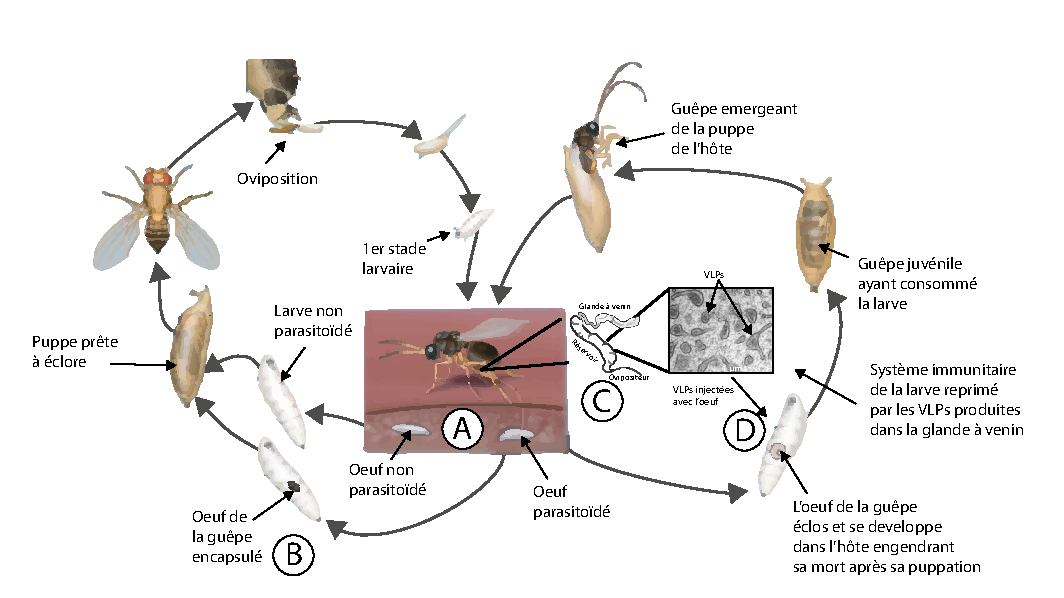
\includegraphics[width=\linewidth,height=\textheight,keepaspectratio]{PhD-master/figures/Leptopilina_lifecycle.pdf}
\caption[Intro:Récapitulatif du cycle de vie d'une espèce de \textit{Leptopilina}]{\textbf{Récapitulatif du cycle de vie d'une espèce de \textit{Leptopilina} modifié à partir du poster d'Amy C. Driskell et al.}}
\label{figure:Leptopilina_lifecycle}
\end{figure}


Aussi, face à cette réponse de l'hôte, les \textit{Leptopilina} ont également trouvé des stratégies pour empêcher l'élimination de leurs œufs. L'une de ces stratégies implique en effet la domestication de gènes viraux qui permettent de produire des VLPs (Virus-like particules) \citep{rizki_parasitoid_1990}. Ces VLPs sont produites dans la glande à venin de la guêpe et sont dépourvues d'ADN, mais contiennent plutôt des protéines de virulence (\figurename{\ref{figure:Leptopilina_lifecycle}}-C). Ces VLPs sont injectées au côté de l'œuf dans la larve de drosophile \citep{colinet_convergent_2007} (\figurename{\ref{figure:Leptopilina_lifecycle}}-D). Une fois injectées dans l'hôte de la guêpe, les VLPs délivrent leur contenu dans les lamellocytes (cellules impliquées dans l'encapsulation) de l'hôte, ce qui modifie principalement leur forme en affectant le cytosquelette, rendant incapable la cellule d'adhérer à l'œuf de parasitoïde \citep{rizki_parasitoid_1990, colinet_convergent_2007} (\figurename{\ref{figure:Leptopilina_VLPs}} - figure en bas à droite). De plus, il a été montré que l'infestation par \textit{L. heterotoma}/ \textit{L. victoriae} provoque également l'apoptose des hémocytes \citep{chiu_natural_2002}.

%\begin{figure}[!htpbt]
%\captionsetup{font=footnotesize}
% \centering
%  \includegraphics[width=\linewidth,height=\textheight,keepaspectratio]{PhD-master/figures/Naldaviricetes_phylogeny.pdf}
%\caption[Intro:Phylogénie des \textit{Naldaviricetes}]{\textbf{Phylogénie des \textit{Naldaviricetes}}}
%\label{figure:Naldaviricetes_phylogeny}
%\end{figure}


L'ancêtre viral responsable de la production de VLPs chez les espèces du genre \textit{Leptopilina} a été récemment identifié comme un proche parent d'un virus filamenteux observé chez \textit{L. boulardi} (LbFV) (Di Giovanni et al., 2020). Parmi les milliers de gènes présents dans le génome de trois espèces (\textit{L.boulardi}, \textit{L.heterotoma} et \textit{L.clavipes}), 13 présentaient des homologies de séquences convaincantes avec 13 ORFs du génome de LbFV. Ces 13 éléments viraux endogènes (EVEs) proviennent très probablement du même événement d'endogénisation ancestral, car leur distribution le long des génomes de trois espèces de \textit{Leptopilina} comprend quelques blocs synténiques et la phylogénie des gènes est parfaitement congruente avec celles des espèces (Di Giovanni et al., 2020) (\figurename{\ref{figure:Leptopilina_VLPs}}). Ces EVEs sont spécifiquement exprimés dans la glande à venin au début du stade nymphal, lorsque les VLPs sont synthétisées. Chose surprenante par rapport aux cas déjà connus chez les polydnavirus  d'Ichneumonoidea, l'amplification génomique d'une partie des EVEs  (10/13) est vraisemblablement régie par une ADN polymérase virale (LbFV\_ORF58) ce qui  entraîne une modulation de leur profil d'expression (\figurename{\ref{figure:Leptopilina_VLPs}}) (Di Giovanni et al., 2020). Plusieurs de ces gènes codent des protéines ayant des fonctions connues chez les virus, dans la transcription (\textit{lef-4}, \textit{lef-8}, et \textit{lef-9}), la réplication de l'ADN (\textit{DNApol}, \textit{helicase}), l'enveloppement des protéines de virulence (\textit{ac81}), et la formation de membranes lipidiques (\textit{lcat}). De plus, l'absence des gènes nécessaires à la production de la capside est cohérente avec l'absence de capside chez les VLPs. Comme on pourrait s'y attendre, les 13 EVEs sont tous soumis à une forte pression de sélection purificatrice (\textit{dN/dS} << 1). De plus, l'un de ces EVEs (LbFV\_ORF85) a été retrouvé par des approches de protéomiques dans les VLPs purifiés, ce qui corrobore leur implication dans leur production (Di Giovanni et al., 2020). Ces VLPs, chez \textit{L.boulardi} ont un rôle essentiel dans le succès reproducteur des guêpes puisqu'ils désactivent les lamellocytes de l'hôte en modifiant leur morphologie  \citep{rizki_parasitoid_1990, colinet_convergent_2007} (\figurename{\ref{figure:Leptopilina_VLPs}}).

\begin{figure}[!htpbt]
\captionsetup{font=footnotesize}
 \centering
  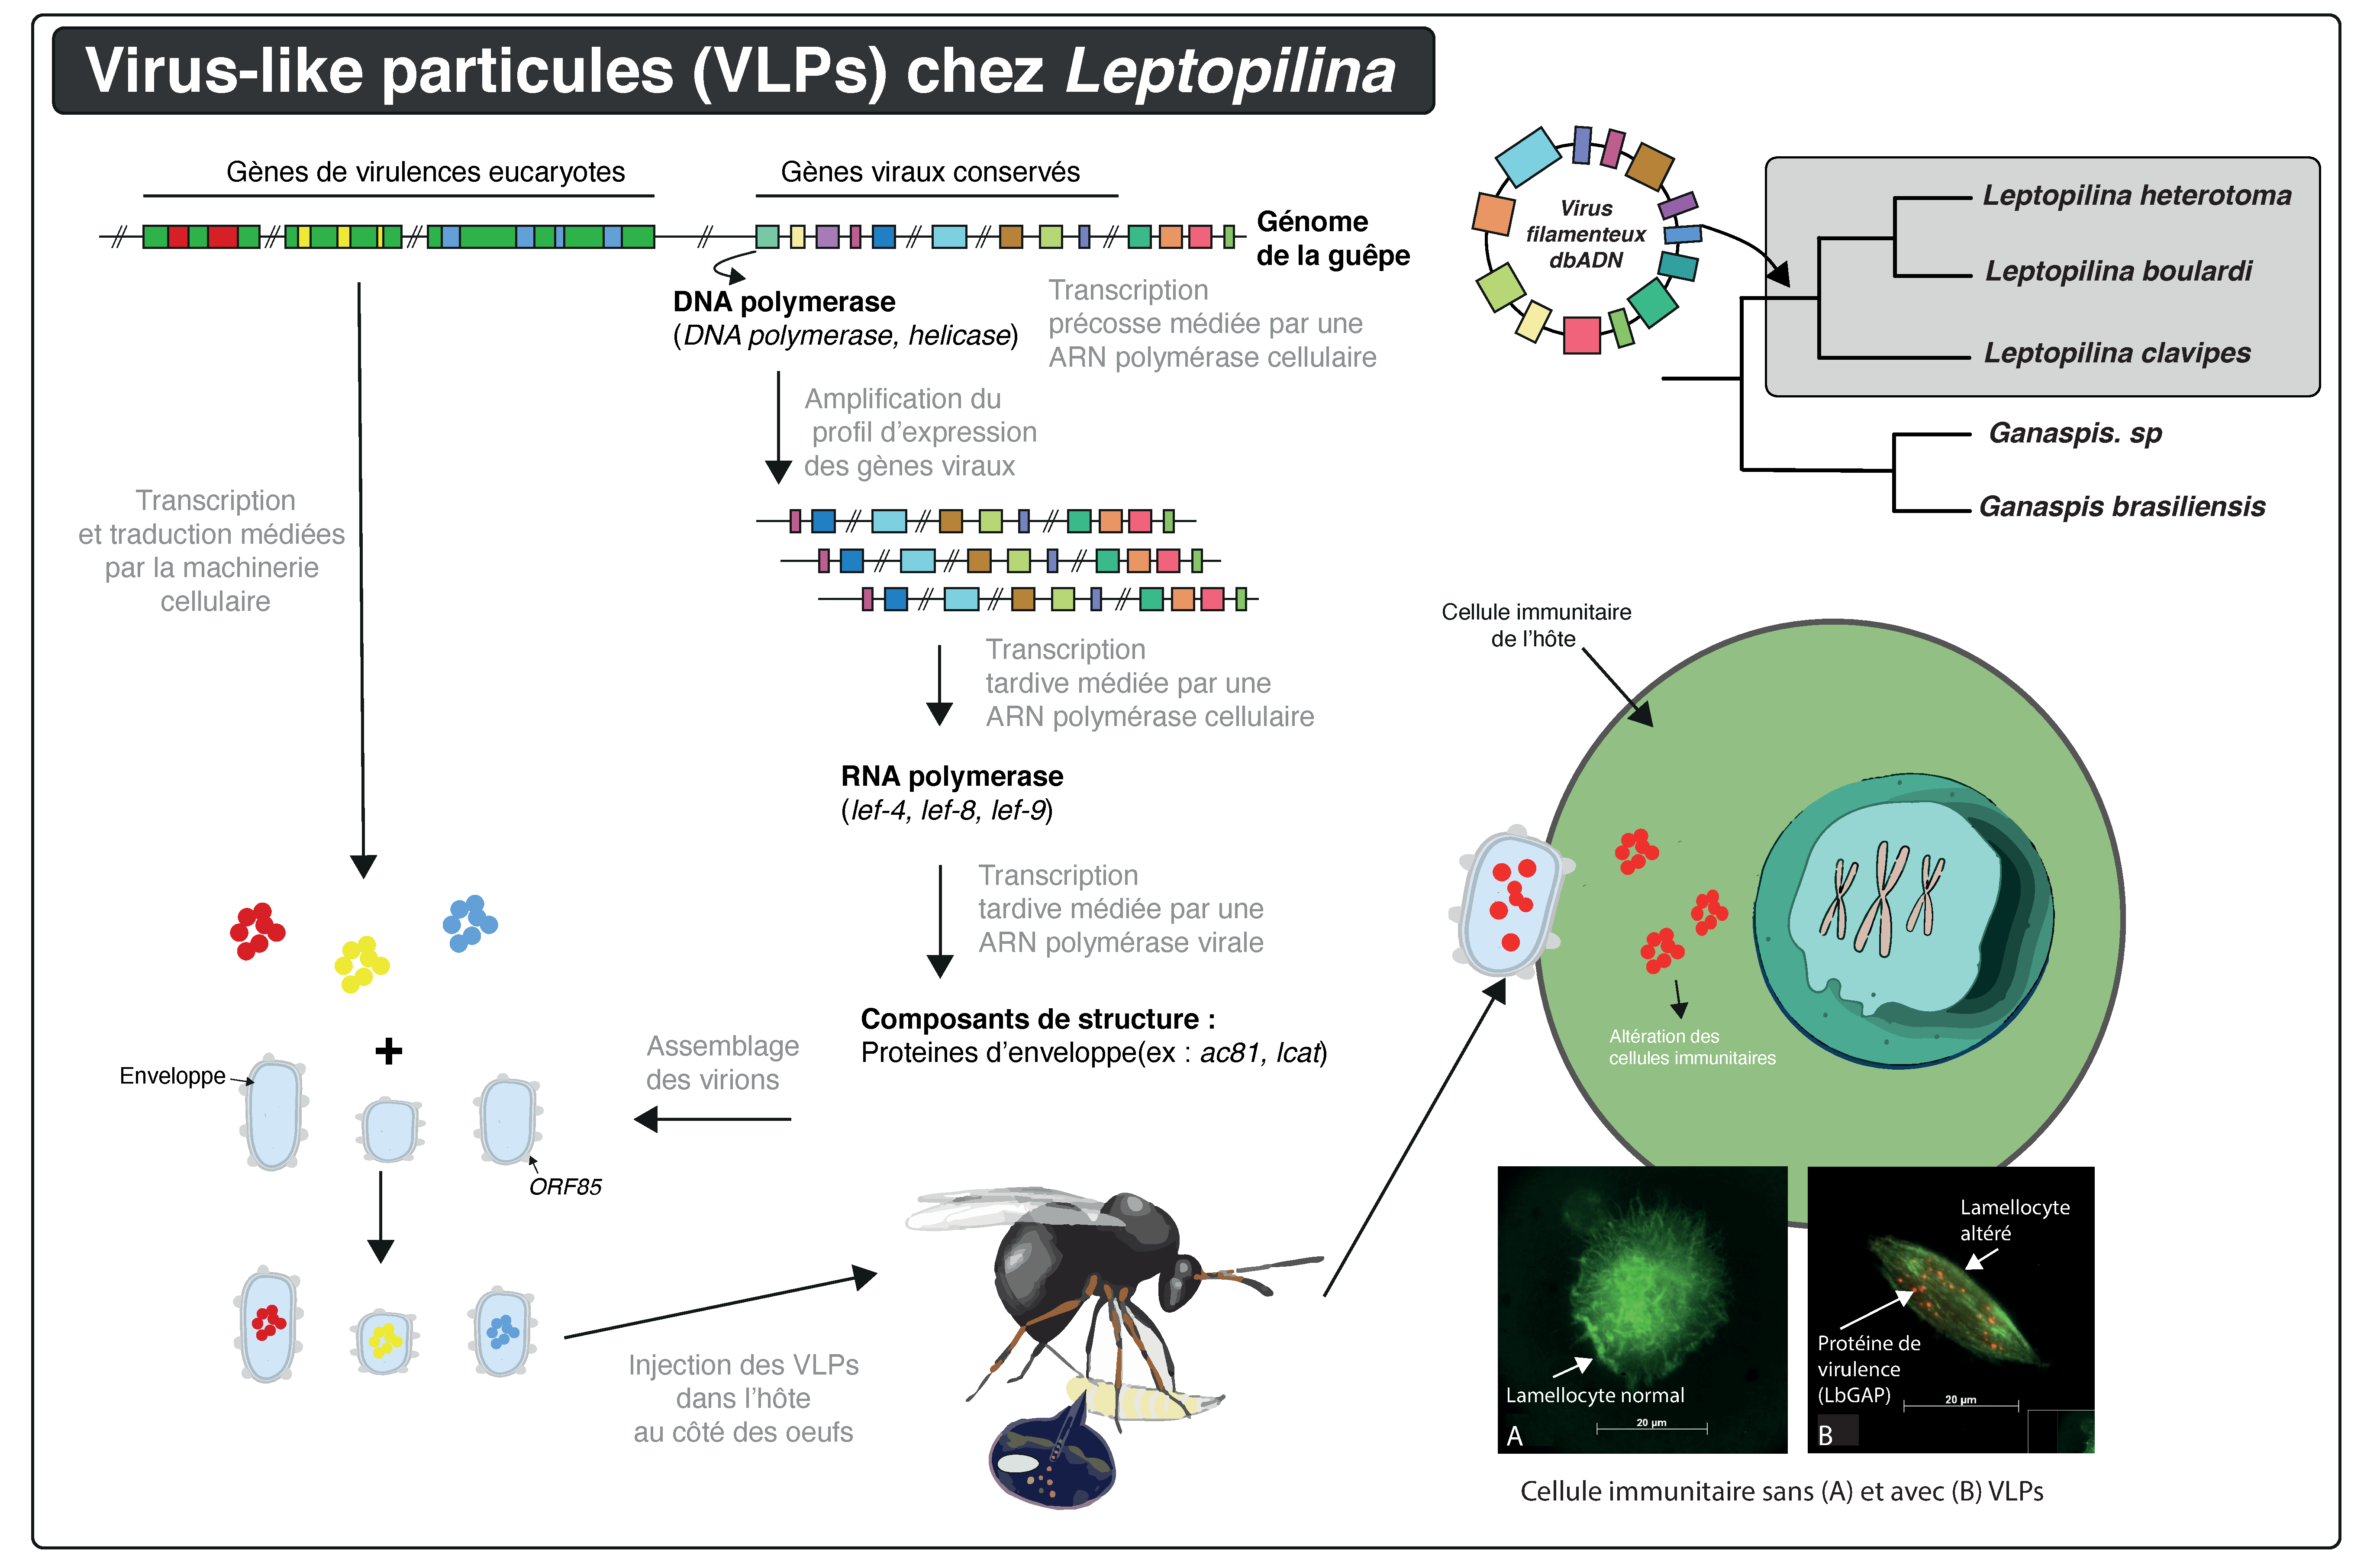
\includegraphics[width=\linewidth,height=\textheight,keepaspectratio]{PhD-master/figures/Leptopilina_VLPS.pdf}
\caption[Intro:Récapitulation du fonctionnement putatif des VLPs chez les espèces de \textit{Leptopilina}]{\textbf{Récapitulation du fonctionnement putatif des VLPs chez les espèces de \textit{Leptopilina}} (photo de \cite{colinet_convergent_2007})}
\label{figure:Leptopilina_VLPs}
\end{figure}

Jusqu'à présent, tous les membres du genre \textit{Leptopilina} (6 examinés) se sont révélés positifs pour la présence d'EVEs homologues à des ORFs de LbFV et produisent toutes des VLPs pour protéger leurs descendants (Di Giovanni et al., 2020). D'autres espèces éloignées des \textit{Leptopilina} mais de la même sous-famille (Eucoilinea) du genre \textit{Ganaspis} (Di Giovanni et al., 2020) n'ont quant à elles présentées aucune homologie avec des ORFs de LbFV et aucun VLPs n'ont été décrits (\figurename{\ref{figure:Figitidae_diversity_intro}}).

\begin{figure}[H]
\captionsetup{font=footnotesize}
 \centering
  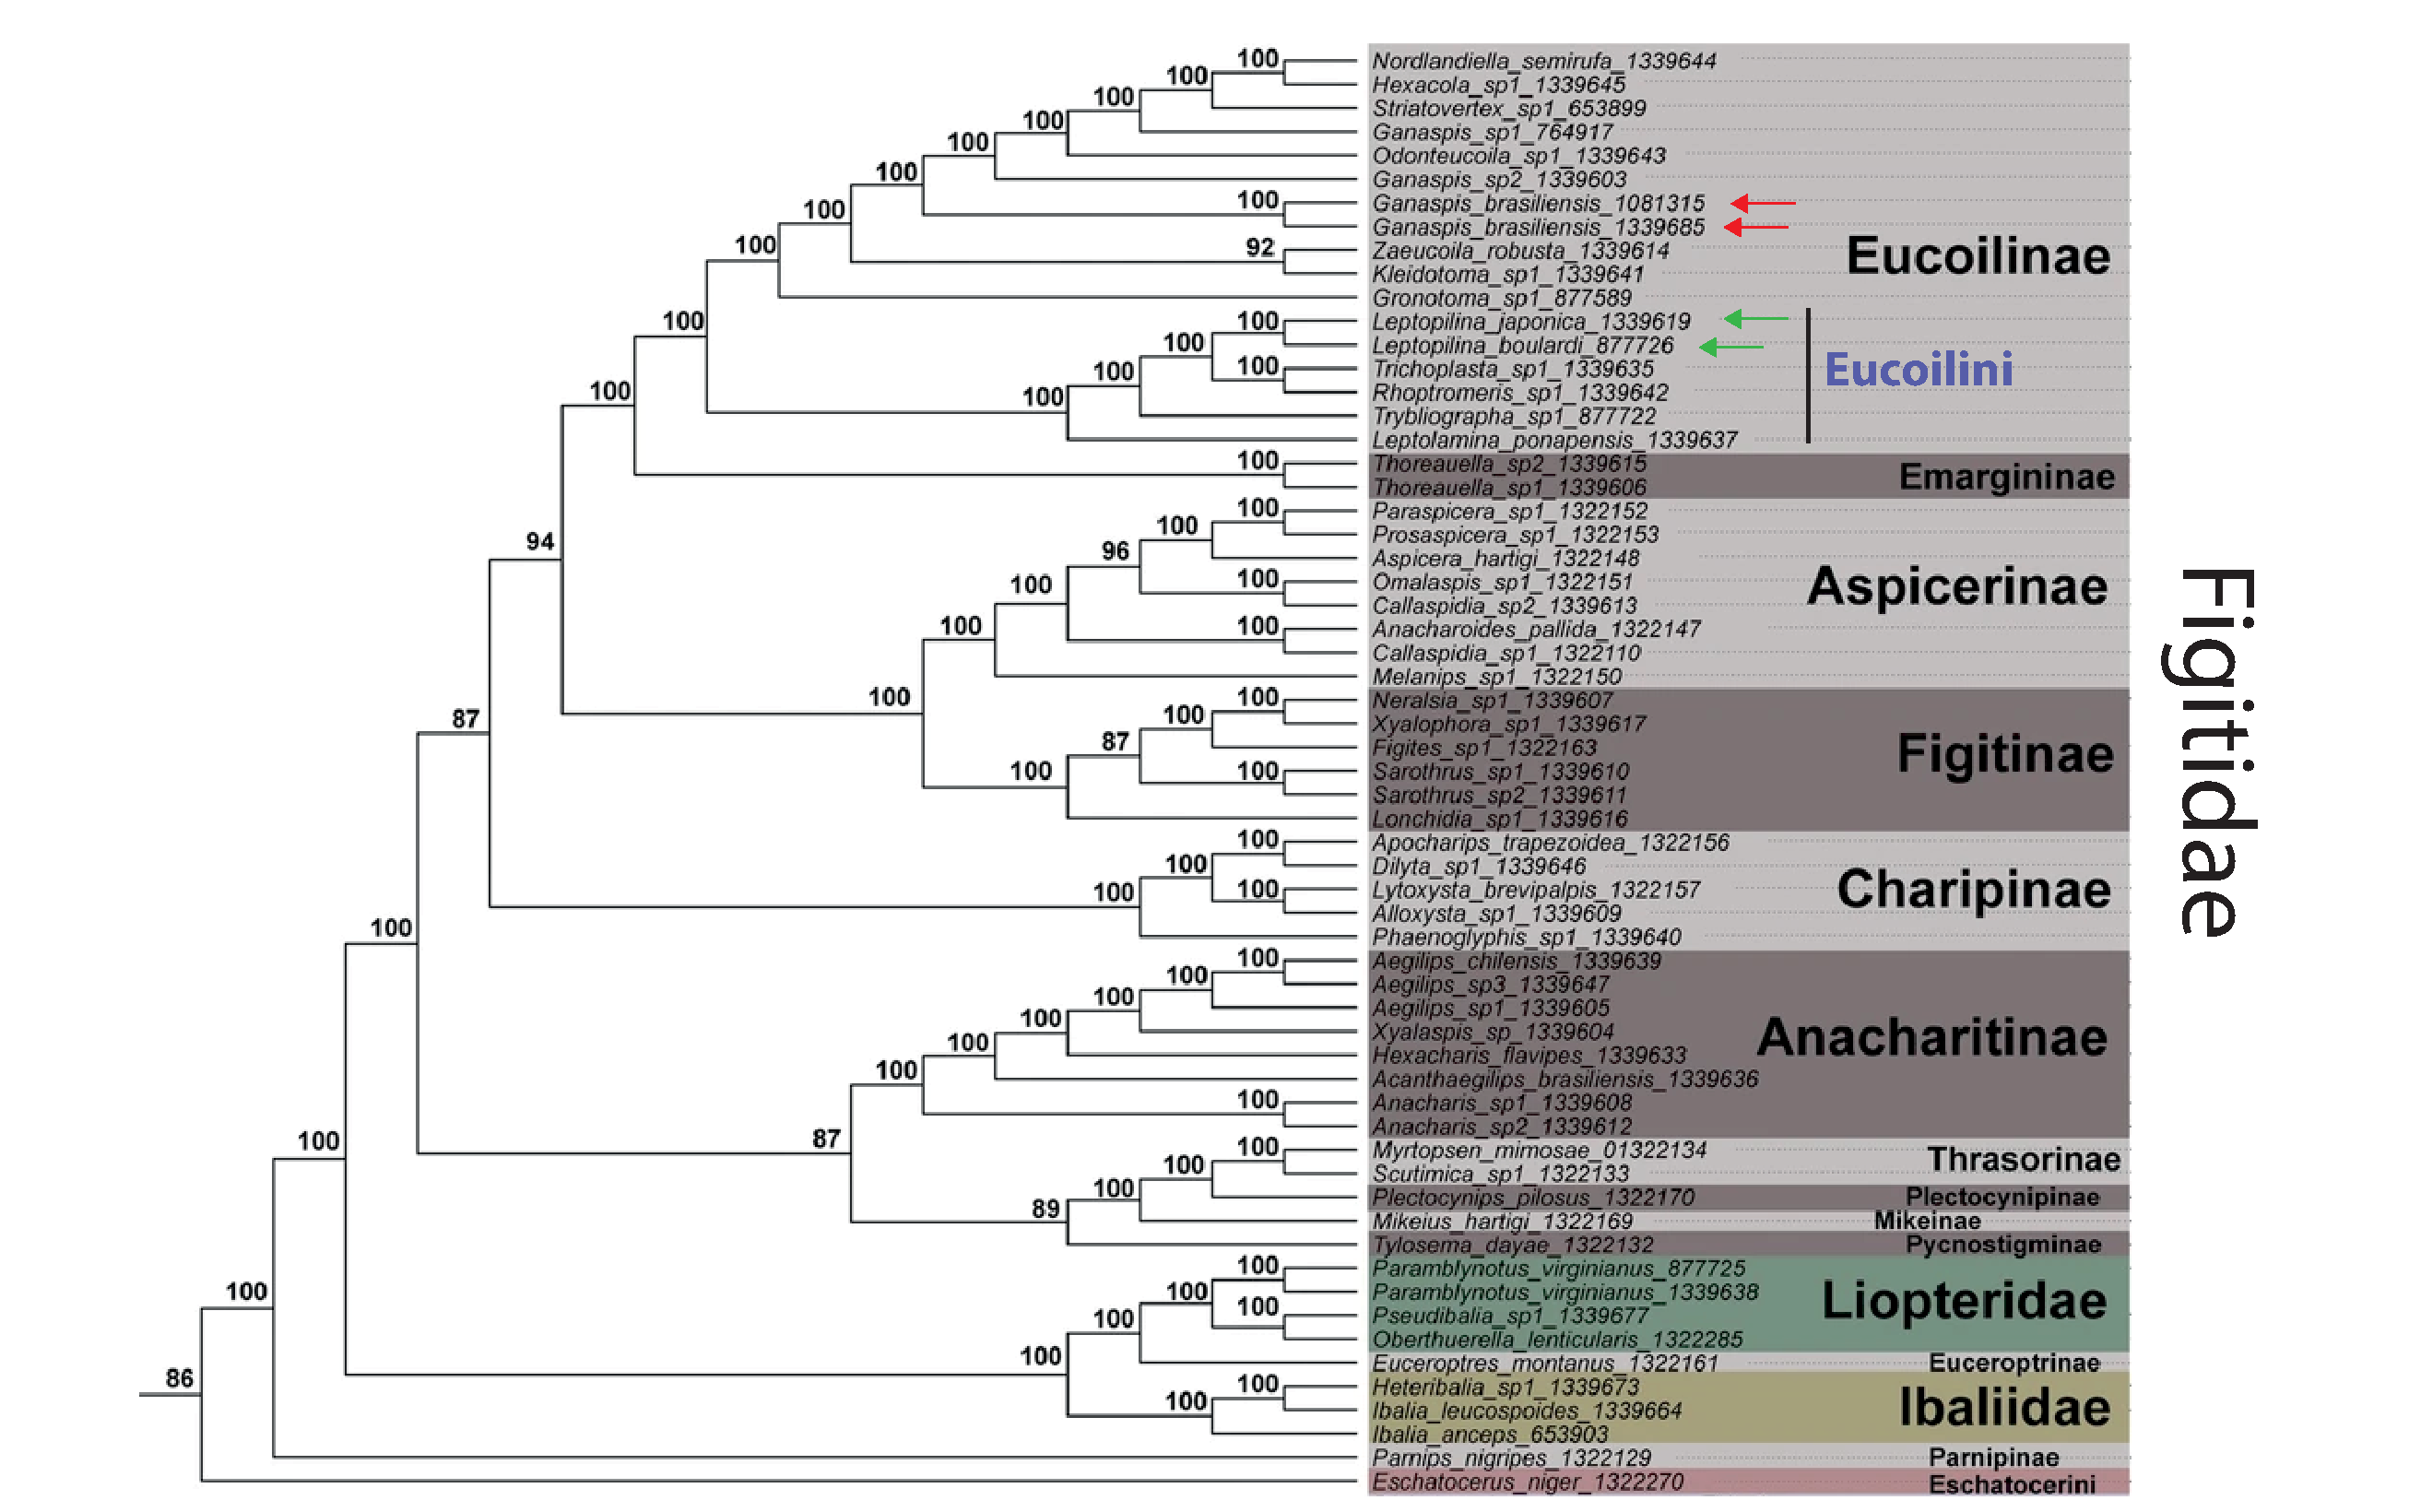
\includegraphics[width=\linewidth,height=\textheight,keepaspectratio]{PhD-master/figures/Figitidae_diversity_intro.pdf}
\caption[Intro:Arbre phylogénétique de la diversité des espèces de la famille des Figitidae]{\textbf{Arbre phylogénétique de la diversité des espèces de la famille des Figitidae}. Les flèches vertes correspondent à la présence d'EVEs homologues à LbFV tandis que les flèches rouges correspondent à l'absence d'homologie (source de \cite{blaimer_comprehensive_2020})}
\label{figure:Figitidae_diversity_intro}
\end{figure}

D'autres EVEs putatifs liés au LbFV ont été trouvés chez d'autres espèces endoparasitoïdes, comme chez \textit{Dolichomitus sp} (Ichneumonidae) \citep{burke_presence_2021} et \textit{Cotesia vestalis} \citep{burke_presence_2021} (\figurename{\ref{figure:Virus_arthropods_phylogeny}}-B), mais ces espèces sont trop éloignées des espèces de \textit{Leptopilina} pour faire partie du même événement d'endogénisation, de plus leur caractère intégré n'est pas réellement clair, surtout concernant \textit{Dolichomitus sp} dans lequel une forme intégrée et libre seraient présentes dans les données \citep{burke_endogenization_2020}. Cela signifie donc que l'événement d'endogénisation s'est produit après la divergence de l'ancêtre commun des espèces \textit{Ganaspis} et \textit{Leptopilina}, il y a environ 91 millions d'années \citep{blaimer_comprehensive_2020} et avant la divergence des espèces \textit{Leptopilina}, il y a environ 41,7 millions d'années \citep{blaimer_comprehensive_2020}. 

Au final, nous manquons de détails sur la gamme d'espèces concernées par cet événement, ainsi que sur l'histoire évolutive de ces virus et leur rôle putatif dans l'évolution de des Figitidae.
    \chapter{Objectifs de thèse}
{\hypersetup{linkcolor=GREYDARK}\minitoc}
\label{chap:intro-objectifs}

\section{Le parasitoïdisme comme facteur explicatif de la variabilité d'endogénisation et domestication chez les Hyménoptères}

Aujourd'hui, les événements d'endogénisation virale commencent à être bien documentés \citep{ter_horst_endogenous_2019, cheng_nudivirus_2020,kondo_novel_2019,irwin_systematic_2022,li_hgt_2022,flynn_assessing_2019}. À l'échelle des insectes, le paysage des EVEs est très variable entre les espèces \citep{gilbert_diversity_2022}. Jusqu'à présent, la taille du génome ainsi que la qualité des assemblages étaient les seuls facteurs proposés pour expliquer cette variabilité. En plus de ces facteurs, nous pourrions également tester l'impact de facteurs écologiques. En effet, les Hyménoptères ayant des habitudes endoparasitaires semblent présenter une plus grande propension à endogéniser et domestiquer des entités virales comparées à des espèces au style de vie ectoparasitaires (pondant leurs œufs sur un hôte) ou des espèces vivant librement tels que les fourmis ou les abeilles. Cette hypothèse est motivée par un ensemble d'études de cas documentant les 6 domestications virales évoquées précédemment chez les guêpes endoparasitoïdes \citep{volkoff_analysis_2010,beliveau_genomic_2015-1,pichon_recurrent_2015,burke_rapid_2018,di_giovanni_behavior-manipulating_2020}. Ces 6 cas concernent exclusivement des endoparasitoïdes et des virus donneurs à génome à ADN double brin.

Face à ces observations, nous proposons à travers le (\hyperref[sec:chap1]{chapitre1}) d'aborder plusieurs questions. 

(1) La première partie de la thèse vise à tester si le phénomène d'endogénisation et de domestication virale est un phénomène plus largement répandu chez les Hyménoptères en élargissant notre point de vue et incluant un panel plus représentatif d'espèces réparties dans la diversité des Hyménoptères. (2) Ensuite, nous proposons de tester si la propension à endogéniser et domestiquer du matériel génétique viral est lié ou non aux virus donneurs puisque jusqu'à présent, ces phénomènes particuliers de domestication semblent impliquer uniquement des virus à grand génome à ADN double brins (dsDNA). (3) Enfin, puisque jusqu'à présent l'ensemble des cas de domestications virales ont été liés à des espèces au style de vie endoparasitoïdes, nous proposons de tester l'hypothèse selon laquelle le style de vie pourrait être un facteur explicatif de la variabilité d'endogénisation et de domestication chez les Hyménoptères. 
%Dans le cas d'un rejet de l'hypothèse nulle (cf. pas d'effet du style de vie), nous pourrions conclure 
Nous nous attendons à ce que les espèces endoparasitoïdes présentent une propension plus grande à endogéniser et/ou domestiquer du matériel génétique viral comparé à des espèces au style de vie libre ou ectoparasitoïde, et ceci pour plusieurs raisons : 

La première raison vient de l'intimité de l'interaction entre l'œuf ou la larve du parasitoïde et l'hôte. En d'autres termes, le mode de vie endoparasitaire pourrait faciliter l'acquisition de nouveaux virus provenant des hôtes du fait de cette proximité. De plus, le mode de vie endoparasitoïde pourrait également faciliter le maintien et la propagation des virus nouvellement acquis au sein des populations de guêpes. En effet, les guêpes endoparasitoïdes injectent souvent non seulement des œufs, mais aussi des composés venimeux (typiquement produits dans la glande à venin ou dans les cellules du calice) où des virus peuvent être présents et peuvent donc être transmis verticalement \citep{martinez_additional_2016, coffman_viral_2022, stasiak_characteristics_2005}.  En outre, le confinement de plusieurs guêpes en développement au sein d'un même hôte peut faciliter la transmission horizontale de ces virus (par exemple \cite{varaldi_infectious_2003}).

La deuxième raison est  liée à l'intensité de la pression de sélection exercée par le système immunitaire de l'hôte sur les endoparasitoïdes. Cette pression sélective peut favoriser la cooptation de fonctions virales telles que l'activité de fusion membranaire mentionnée ci-dessus, qui constitue un moyen très efficace pour délivrer des facteurs de virulence. 

Afin de tester ces hypothèses, j'ai développé un pipeline bioinformatique pour détecter les événements d'endogénisation impliquant tout type de virus (ADN/ARN, simple brin, double brin), à l'échelle de l'ensemble de l'ordre des Hyménoptères. Cette analyse nous a d'abord permis de tester si la propension des virus à entrer dans les génomes des Hyménoptères, et à être domestiqués, dépend de leur structure génomique.  Nous avons ensuite testé si le mode de vie de l'espèce (vivant librement, endoparasitoïde, ectoparasitoïde) est en corrélation avec sa propension à intégrer et à domestiquer des virus.

\section{Description d'une nouvelle famille de virus : les Filamentoviridae}

Depuis les années 1970, des études en microscopie électronique, ont mis en évidence une variété de virus dans le système reproducteur de guêpes parasitoïdes. En effet, plusieurs espèces de guêpes endoparasitoïdes présentaient des particules enveloppées en forme de bâtonnets flexibles à l'allure filamenteuse, ce qui leur a valu le nom de "virus filamenteux". Leur nature est néanmoins restée un mystère en raison du manque de données génétiques les concernant. De tels virus ont par exemple été décrits chez un Campopleginae (\textit{Diadegma terebrans} \citep{krell_replication_1987}), une série de  Braconidae (\textit{Cotesia congregata} \citep{de_buron_characterization_1992}, \textit{Cotesia hyphantriae}, \textit{Cotesia marginiventris} \citep{hamm_comparative_1990},  \textit{Microplitis rufiventris} \citep{hegazi_calyx_2005}) et un Figitidae (\textit{Leptopilina boulardi} \citep{varaldi_infectious_2003}).

Ce dernier virus que l'on retrouve chez \textit{Leptopilina boulardi} possède une biologie étonnante. Il s'agit d'un virus hérité verticalement de la mère aux progénitures se nommant Leptopilina boulardi filamentous virus (LbFV) en rapport à son hôte. Il manipule le comportement de ponte des femelles parasitoïdes en induisant du "superparasitisme" (ponte d'œufs dans des hôtes déjà parasités) \citep{varaldi_infectious_2003,varaldi_artifical_2006}. Cette modification du comportement favorise la transmission horizontale du virus au sein des larves de drosophile superparasitées. Cette modification du comportement est adaptative du point de vue du virus et coûteuse pour le parasitoïde \citep{gandon_superparasitism_2006}, ce qui fait de cette modification comportementale un exemple de "manipulation" induite par un virus.

C'est en 2017 que le premier "virus filamenteux", LbFV a été séquencé chez \textit{Leptopilina boulardi} \citep{lepetit_genome_2017}. Ce virus est par ailleurs apparenté au virus s'étant intégré chez les espèces du genre \textit{Leptopilina} et ayant mené à la domestication des 13 EVEs évoqués précédemment \citep{di_giovanni_behavior-manipulating_2020}. L'analyse phylogénétique l'a clairement identifié comme un membre de la classe des \textit{Naldaviricetes} (classe de virus à dsDNA infectant les arthropodes) dont la famille la plus proche est celle des \textit{Hytrosaviridae}. Néanmoins, en raison d'une divergence élevée avec les \textit{Hytrosaviridae}, il a été proposé que ce virus appartienne à une famille distincte au sein des \textit{Naldaviricetes}  \citep{lepetit_genome_2017}, dont il est le seul représentant.

Dans le \hyperref[sec:chap1]{chapitre 1}, pendant que je recherchais la présence systématique d'éléments viraux endogénisés dans les génomes d'Hyménoptères, nous avons également pu caractériser un certain nombre d'éléments viraux exogènes de virus ADN qui présentaient des signaux caractéristiques de virus libres. Ces virus à génome ADN correspondent à des virus ayant été séquencés au même moment que le génome de l'Hyménoptère. Nous avons ainsi pu découvrir chez 3 espèces de guêpes endoparasitoïdes, une vingtaine de scaffolds appartenant à 3 nouveaux virus libres proches phylogénétiquement de LbFV. Par ailleurs, nous avions aussi en notre possession le génome du virus LhFV retrouvé chez \textit{Leptopilina heterotoma} suite à une purification effectuée dans notre laboratoire.  Au même moment, l'équipe IRBI de Tours faisait des découvertes connexes chez une autre espèce de guêpes endoparasitoïdes où deux nouveaux virus ont été découverts.

C'est ainsi que le \hyperref[sec:chap1]{chapitre 2} est né d'une collaboration étroite avec l'IRBI de Tours, permettant de réunir des compétences et expériences variées. Dans cette collaboration, nous effectuons des analyses génomiques et phylogénétiques comparatives approfondies de ces six nouveaux virus filamenteux découverts chez cinq espèces d'Hyménoptères endoparasitoïdes.  Dans ce travail, des virus "filamenteux" infectant des guêpes appartenant à quatre super-familles et 5 genres : \textit{Leptopilina} (Cynipoidea), \textit{Encarsia} (Chalcidoidea), \textit{Platygaster} (Platygastroidea), \textit{Psyttalia}, et deux souches de \textit{Cotesia} (Ichneumonoidea). 

En utilisant des analyses phylogénétiques, génomique, et de morphogenèse des particules, nous montrons que les membres de cette nouvelle famille de virus filamenteux partagent quelques traits singuliers. Ces résultats apportent des arguments qui soutiennent l'hypothèse que les virus filamenteux constituent une famille de virus distincte au côté des \textit{Hytrosaviridae}. Ce travail constitue donc la base préliminaire à leur classification dans l'ICTV an tant que nouvelle famille que nous proposons de nommer Filamentoviridae en lien à leur structure filamenteuse, formant ainsi la cinquième famille de la classe des \textit{Naldaviricetes}.

\section{Caractérisation de l'évènement de domestication chez les \textit{Leptopilina} et estimation de l'âge des Filamentoviridae}.

Dans ce dernier travail de thèse (\hyperref[sec:chap1]{chapitre 3}), je me suis focalisé sur une échelle plus fine. Cette échelle est celle de la famille des Cynipoidea, une famille de guêpes endoparasitoïdes comprenant les \textit{Leptopilina}.  Nous venons de le voir, c'est précisément chez les espèces du genre \textit{Leptopilina} que se trouve le cas le plus récemment documenté de domestication de plusieurs gènes viraux (13). Ces gènes sont impliqués dans la synthèse des VLP, qui, lorsqu'elles sont injectées au côté des œufs, protègent la progéniture de la femelle du système immunitaire de l'hôte \citep{di_giovanni_behavior-manipulating_2020}. Ces 13 EVE domestiqués (dEVEs) sont issus d'un seul et même évènement d'intégration dont les gènes sont phylogénétiquement liés au virus filamenteux Leptopilina boulardi filamentous virus (LbFV) et proviennent donc d'un virus ancestral appartenant à la nouvelle famille des Filamentoviridae que nous décrivons dans le \hyperref[sec:chap1]{chapitre 2}. Avec ces nouveaux éléments, nous avions l'opportunité d'entrer dans le domaine de la paléovirologie. En effet, en étudiant ces virus anciens, figés dans les génomes des guêpes, nous pouvions maintenant décrire à la fois l'histoire évolutive de l'acquisition de ces gènes viraux (quand est-ce que l'endogénisation a eu lieu, et quelle est la diversité de guêpes impliquées ?), mais également en déduire la période d'apparition des virus de la famille des Filamentoviridae.

Pour mener ce projet, nous avons sondé les génomes de plusieurs espèces de la famille des Figitidae à laquelle appartiennent les \textit{Leptopilina}. Le jeu de donnée présentait 41 individus représentant 20 genres différents répartis en 6 sous-familles. 


%Les extractions d'ADN et l'amplification et le séquençage d'un produit PCR d'un ORF très conservé parmi les 13 nous ont permis de montrer que l'évènement concernait au moins les genres \textit{Leptopilina} et \textit{Trybliographa}, appartenant tous deux à la sous-famille des Eucoilinae (tribu des Eucoilini). Nous avons ensuite poursuivi l'analyse en échantillonnant, extrayant et séquençant le génome de 4 autres genres d'Eucoilinae (\textit{Rhoptromeris sp}, \textit{Leptolamina sp}, et \textit{Thrichoplasta sp}). Ces résultats nous ont permis d'inférer un évènement d'endogénisation ayant eu lieu après la divergence entre les \textit{Leptolamina} (espèce basale du groupe Eucoilini) et le reste du groupe, puisqu'aucune trace d'endogénisation n'a été détectée chez ce dernier tandis que l'ensemble des 13 gènes domestiqués ont été retrouvés dans les génomes des trois autres espèces. 

%Enfin, la caractérisation dans le temps de cet évènement d'endogénisation nous a permis de calibrer la phylogénie des virus libres s'étant intégré chez l'ancêtre commun de ces guêpes. En effet, puisque la phylogénie des 13 EVEs coïncide parfaitement avec celle des hôtes depuis l'ancêtre commun, la divergence des nœuds estimés chez les guêpes nous permet d'obtenir des points de calibration sur la phylogénie des virus \textit{Naldaviricetes} et ainsi d'estimer l'âge des différentes familles qui constituent ce clade. 

%Enfin, la caractérisation dans le temps de cet évènement d'endogénisation nous a permis de calibrer la phylogénie des virus apparentés au virus s'étant intégré il y a 75 millions d'années. En effet, puisque la phylogenèse des 13 EVEs coïncide parfaitement avec celle des hôtes depuis l'ancêtre commun, la divergence des nœuds estimés chez les Eucoilinae peut permettre d'obtenir des points de calibration sur la phylogénie des \textit{Naldaviricetes}. Ainsi, nos résultats coïncidents et précisent les estimations proposées en 2011 par \cite{theze_paleozoic_2011} pour la divergence des familles de \textit{Baculoviridae} et \textit{Nudiviridae}, il y a 348 millions d'années. Ces résultats permettent également de proposer une date de divergence de la classe des \textit{Naldaviricetes}, il y a 421 millions d'années, et celle de la famille des \textit{Filamentoviridae}, il y a 317 millions d'années. Aussi, c'est vraisemblablement à l'éon phanérozoïque, qui s'étend sur 538,8 millions d'années jusqu'à aujourd'hui, au cours duquel une vie animale et végétale abondante ont existé, que les grands virus à dsDNA de ce groupe auraient existé et auraient commencé à se diversifier et se spécialiser chez divers hôtes d'insectes.

    \part{Résumés des études}
    \label{part:studies}
    
    \thispagestyle{empty}
    \chapter{L'endoparasitoïdisme favorise l'endogénisation et la domestication des virus à dsDNA}

Le transfert de gènes entre organismes non apparentés a été découvert comme une source importante d'innovation génétique, qui peut parfois aboutir à de l'adaptation. Ces transferts horizontaux de gènes (THG) sont courants chez les procaryotes, et leurs effets sont reconnus depuis longtemps. Des travaux récents suggèrent que les eucaryotes peuvent également être engagés dans ces processus \citep{irwin_systematic_2022}. Cependant, les paramètres qui déterminent la structure des THGs impliquant des eucaryotes restent inconnus.\\

Dans cette étude, nous faisons l'hypothèse que le mode de vie des Hyménoptères est un facteur structurant les chances d'endogénisation des gènes viraux. Plusieurs séries d’études documentant des évènements de domestications de machineries virales entières exclusivement par des guêpes endoparasitoïdes ont motivé cette hypothèse. Dans tous les cas décrits, des structures de type virales codées par des gènes de virus à dsDNA permettent d’adresser des facteurs de virulence qui protègent les progéniteurs des guêpes du système immunitaire de leur hôte \citep{bezier_polydnaviruses_2009,volkoff_analysis_2010,burke_common_2019,pichon_recurrent_2015,di_giovanni_behavior-manipulating_2020}. \\

À partir de ces données, notre hypothèse de travail est que le mode de vie endoparasitoïde peut être associé à un taux plus élevé d'endogénisation virale et/ou à un taux plus élevé d'événements de domestication, pour deux raisons non exclusives impliquant (i) l'exposition à de nombreux virus et/ou (ii) la valeur adaptative des éléments endogénisés.\\

Selon le premier argument, un taux plus élevé d'endogénisation peut provenir d'une exposition accrue aux virus. En raison de l'interaction intime entre l'œuf ou la larve d'un endoparasitoïde et son hôte, cet effet pourrait être particulièrement présent chez les endoparasitoïdes. En d'autres termes, l'endoparasitoïsme pourrait faciliter l'acquisition de nouveaux virus auprès des hôtes, ainsi que le maintien et la propagation des virus nouvellement acquis au sein des populations de guêpes, en raison de leur mode de vie unique. En effet, les guêpes endoparasitoïdes injectent fréquemment non seulement des œufs mais aussi du venin (généralement produit dans la glande à venin ou les cellules du calice) où peuvent se loger des virus, profitant ainsi d'une transmission verticale, facilitant ainsi leur propagation verticale \citep{martinez_additional_2016,coffman_viral_2022}. De plus, le confinement de plusieurs guêpes en développement au sein d'un seul hôte peut faciliter la transmission horizontale du virus et la propagation ultérieure de la population parmi les guêpes (par exemple, \citep{varaldi_infectious_2003,coffman_viral_2022}).\\

Selon le second argument, les insertions virales et le taux de domestication serait plus élevés chez les endoparasitoïdes car leur endogénization aurait été sélectionnée positivement. En effet, contrairement à d'autres modes de vie, échapper au système immunitaire de l'hôte est particulièrement difficile à relever pour ces insectes comparés à d'autres Hyménoptères au style de vie ectoparasitoïde par exemple, pour lesquels les progénitures ne sont pas en interaction étroite avec le système immunitaire de l'hôte. Cette pression sélective peut donc favoriser la cooptation de caractéristiques virales, telles que l'activité de fusion membranaire des virus, ce qui peut optimiser la délivrance des facteurs de virulence.\\

Pour tester ces hypothèses, un pipeline bioinformatique a été construit afin de rechercher des EVEs dans des génomes. Celui-ci comporte trois étapes principales. i : la recherche systématique d'éléments viraux endogènes par homologie de séquence avec une base de données exhaustive de protéines virales, ainsi que des indices permettant de tester l'hypothèse d'endogénisation, telles que la couverture de séquençage le long des scaffolds contenant des EVEs ou la proximité avec d'autres éléments génétiques eucaryotes typiques. ii: l'examen de l'histoire évolutive des insertions, qui est comparée à la phylogénie des espèces. Et enfin, iii, l'investigation systématique, si possible, du caractère adaptatif de ces insertions en étudiant le régime de sélection des séquences depuis leur endogénisation par des approches de \textit{dN/dS} ou par l'analyse des profils d'expression. \\

Nous avons appliqué ce pipeline à 124 espèces d'hyménoptères (dont 32 correspondaient à des génomes de parasitoïdes séquencés par le laboratoire). Ces résultats ont permis de découvrir plusieurs nouveaux cas d'endogénisation et de domestication de virus chez les Hyménoptères. Nous montrons dans un premier temps que les virus à dsDNA sont beaucoup plus souvent endogénisés et domestiqués qu'attendu selon la répartition de ces virus chez les insectes (\figurename{\ref{figure:Resume_figure_papier1_1}}).\\

\begin{figure}[!htpbt]
\captionsetup{font=footnotesize}
 \centering
  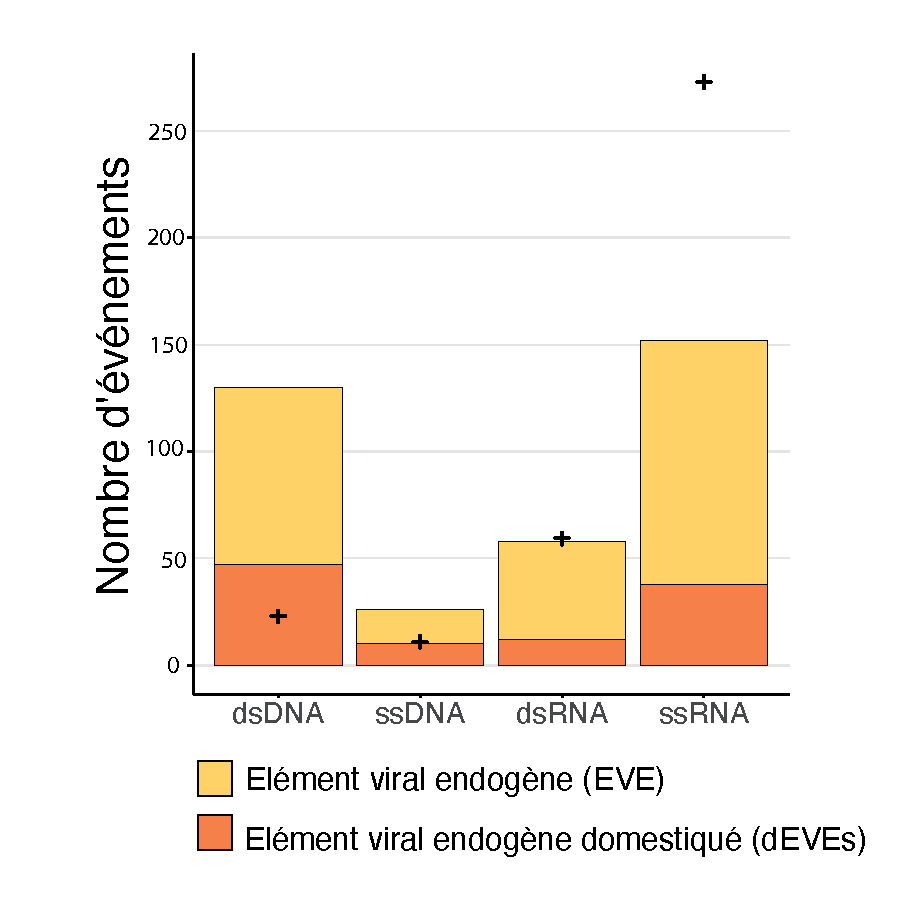
\includegraphics[width=\linewidth,height=\textheight,keepaspectratio]{PhD-master/figures/Resume_figure_papier1_1.pdf}
\caption[Paper1:Figures principales récapitulatives du chapitre1\_1]{\textbf{Distribution des évènements en fonction des structures génomiques}. Distribution du nombre d'événements inférés, selon les quatre catégories de structures génomiques virales. Les croix renvoient au nombre attendu d'événements d'endogénisation pour chaque catégorie en fonction de leur abondance relative estimée chez les insectes en s'appuyant sur les séquences disponibles dans les bases de données (voir les détails dans \hyperref[sec:MM-8]{Matériel et méthodes} et les données sur les virus infectés dans le fichier GitHub : \href{https://github.com/BenjaminGuinet/PhD_defense/blob/main/Supplementary_paper1/All_virus_infecting_insects_informations.csv}{All\_virus\_infecting\_insects\_informations.csv}.}
\label{figure:Resume_figure_papier1_1}
\end{figure}

Pour expliquer ce phénomène, nous pouvons supposer que la prévalence observée des virus à dsDNA est le résultat d'un potentiel de transfert de matériel adaptatif plus important que celui des autres virus (\figurename{\ref{figure:Resume_figure_papier1_1}}). En effet, nous pourrions imaginer que les virus à ADN double brins seraient plus à même à rentrer dans les génomes que les hôtes compte tenu du fait qu'ils présentent des génomes de même structure que ceux des guêpes et que la plupart se répliquent dans le noyau de leurs hôtes. En effet, la réplication nucléaire est une caractéristique partagée par presque toutes les familles de virus à dsDNA trouvées dans notre analyse : \textit{Baculoviridae}, \textit{Iridoviridae}, \textit{Phycodnaviridae}, \textit{Nimaviridae}. \textit{Caulimoviridae}, \textit{Herpesviridae}, \textit{Asfaviridae} \citep{schmid_dna_2014,harrison_ictv_2020,international_committee_on_taxonomy_of_viruses_virus_2012,teycheney_ictv_2020,verbruggen_molecular_2016}, les virus filamenteux d'\textit{Apis mallifera} (AmFV) \citep{clark_filamentous_1978} et le virus filamenteux LbFV \citep{varaldi_artifical_2006} (les \textit{Poxviridae}, qui se répliquent dans le cytoplasme, sont donc la seule exception). \\

\begin{figure}[H]
\captionsetup{font=footnotesize}
 \centering
  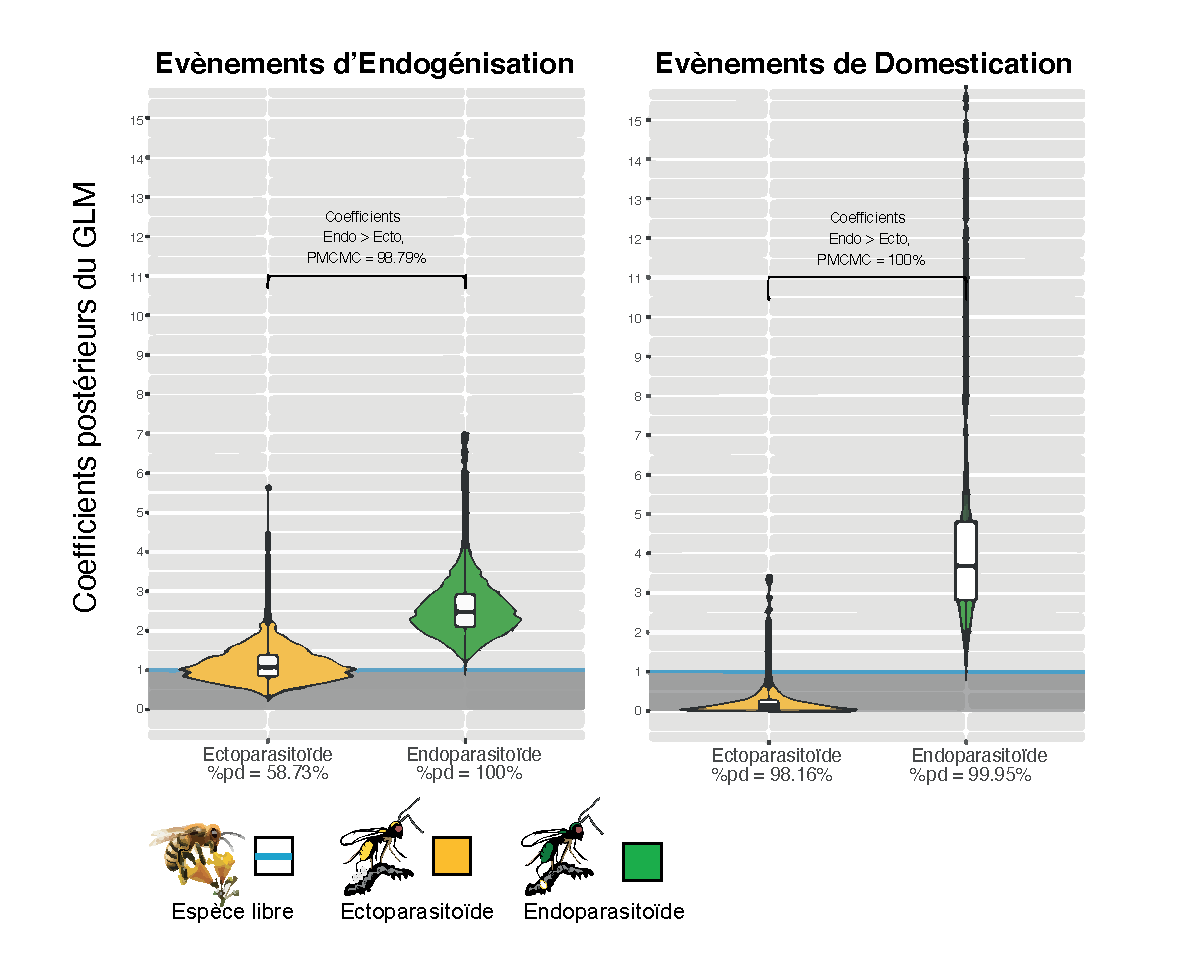
\includegraphics[width=\linewidth,height=\textheight,keepaspectratio]{PhD-master/figures/Resume_figure_papier1_2.pdf}
\caption[Paper1:Figures principales récapitulatives du chapitre1\_2]{\textbf{Distribution des coefficients de taux d'endogénisation et de domestication de virus à dsDNA selon les styles de vie}. Les diagrammes en violon représentent la distribution postérieure des coefficients d'évènements impliquant des virus à dsDNA obtenus sous les différents modèles GLM (après transformation exponentielle pour obtenir un taux relatif aux espèces libres). Les coefficients sont dérivés de 1000 modèles GLM indépendants, où 1000 scénarios probables d'états ancestraux aux nœuds ont été échantillonnés de manière aléatoire parmi les itérations MCMCM (voir les détails dans \hyperref[sec:MM-12]{Matériel et méthodes}). Le \%pd est la probabilité de direction et indique la proportion de la distribution postérieure où les coefficients ont le même signe que le coefficient médian. Le $P_{MCMCM}$ indique la proportion d'itérations MCMC où le coefficient obtenu pour les espèces endoparasitoïdes est plus élevé que pour les espèces ectoparasitoïdes. Tous les résumés statistiques des modèles GLM bayésiens peuvent être trouvés sur le dépôt GitHub sous le nom : \href{https://github.com/BenjaminGuinet/PhD_defense/blob/main/Supplementary_paper1/Lifestyle_statistical_analysis_results.xlsx}{Lifestyle\_statistical\_analysis\_results.xlsx}.}
\label{figure:Resume_figure_papier1_2}
\end{figure}

.\newline
Enfin, nous apportons également des arguments que les guêpes endoparasitoïdes sont plus susceptibles que les ectoparasitoïdes et les espèces libres d'endogéniser et de domestiquer les virus à ADN double brin (\figurename{\ref{figure:Resume_figure_papier1_2}}).\\

Nous pouvons alors essayer de comprendre pourquoi les guêpes endoparasitoïdes subiraient des évènements d'endogénisation plus fréquemment que les espèces libres ou au style de vie ectoparasitoïde. Selon notre première hypothèse, selon laquelle les endoparasitoïdes peuvent présenter plus d'événements d'endogénisation parce qu'ils interagissent avec plus de virus, nous nous attendions que tous les virus, quelle que soit leur structure génétique, bénéficient de cet effet. En particulier, nous devrions observer cet effet chez les virus à ARN, qui sont impliqués dans le plus grand nombre d'événements d'endogénisation. Cependant, seuls les virus à dsDNA présentaient des profils d’endogénisation et de domestication beaucoup plus fréquents que les autres styles de vie. Par conséquent, nous pensons que cette explication est peu probable. \\

Notre deuxième hypothèse était que les endoparasitoïdes seraient sélectionnés pour maintenir des gènes d'origine virale, car leur rétention améliorerait leur valeur selective dans un contexte immunitaire. Dans nos résultats, les événements de domestication sont plus fréquemment observés chez les endoparasitoïdes (plus de 3 fois plus d'évènements que chez les autres Hyménoptères) (\figurename{\ref{figure:Resume_figure_papier1_2}}). Il est clair qu'une partie de ce phénomène peut s'expliquer par l'apport accru indiqué ci-dessus (le taux plus élevé d'endogénisation). Après avoir contrôlé ce facteur, une tendance vers un taux de domestication plus élevé persiste. Plus précisément, la probabilité de domestication après endogénisation était considérablement plus élevée pour les endoparasitoïdes que pour les ectoparasitoïdes, mais pas significativement plus élevée que pour les espèces libres. Cependant, si un seul événement de domestication empêche la domestication d'autres EVE sans affecter le taux d'endogénisation non adaptative, alors on s'attend à de très faibles différences sur cet indice. En effet, cet effet entrainerait la "dilution" du signal lié à la domestication le long des branches. Si cet effet est en jeu, alors notre capacité à détecter toute différence dans les taux de domestication entre les modes de vie est considérablement réduite.\\

Enfin, si les virus à dsDNA sont plus susceptibles d'être domestiqués par les guêpes endoparasitoïdes, c'est peut-être parce que leurs structures génomiques virales sont similaires à celles des guêpes, ce qui les rendrait plus simples à assimiler pour les génomes. De plus, d'autres propriétés des virus à ADN double brin peuvent expliquer ce pattern. En effet, L'ADN qui est emballé dans les particules matures code généralement des protéines de virulence provenant de la guêpe \citep{espagne_genome_2004}. Cela signifie que, au moins pour ces cas, le système viral devrait être capable d'emballer l'ADN, ce qui est très probablement une caractéristique que les virus à ADN peuvent fournir. Cet argument ne tient pas dans les systèmes VLPs, où seules les protéines sont emballées dans les particules virales, et on ne voit pas pourquoi les EVE dérivées de virus à dsDNA seraient plus à même de remplir une telle fonction. D'autres caractéristiques des virus à dsDNA apparaissent ici comme des facteurs potentiellement importants : la grande taille de leur génome et la taille de leur capside et de leur enveloppe \citep{chaudhari_scaling_2021}. Ces caractéristiques pourraient prédisposer les virus à dsDNA à être domestiqués, puisque d'abondantes quantités de venins doivent être transmises afin de supprimer efficacement la réponse immunitaire de l'hôte.\\

En conclusion, nous faisons l'hypothèse que les taux plus élevé d'endogénisation et le plus grand nombre d'événements de domestication de virus dsDNA chez les endoparasitoïdes sont le résultat de l'intense pression sélective exercée par le système immunitaire de l'hôte sur les endoparasitoïdes. Cette pression sélective sévère peut favoriser les endoparasitoïdes qui conservent une machinerie virale qui les aide à s'attaquer aux facteurs de virulence de leurs hôtes. Plus largement, nous estimons que ce phénomène devrait être omniprésent chez les espèces d'insectes ayant un mode de vie similaire.\\


Le manuscrit est actuellement en review dans le journal eLife et est disponible sous forme de preprint sur \href{https://doi.org/10.1101/2022.11.16.515002}{bioRxiv} sous le DOI : 10.1101/2022.11.16.515002.\\

Ces travaux sont également disponibles en anglais reformaté dans la première section du chapitre \hyperref[sec:chap1]{Études}. 

    \thispagestyle{empty}
    \chapter{Proposition d'une nouvelle famille virale associée aux Hyménoptères parasitoïdes}

Dans le chapitre précédent (\hyperref[sec:chap1]{chapitre 1}), nous avons cherché la présence d'éléments viraux endogénisés (EVEs) dans le génome de nombreuses espèces d'Hyménoptères. Le pipeline développé pour cet usage, nous a également permis d'observer la présence de plusieurs éléments viraux exogènes appartenant probablement à des virus à ADN libres séquencés au même moment que les génomes des insectes (pour plus d'informations sur ces éléments exogènes, veuillez vous référer à la section \hyperref[sec:perspective]{perspective} du manuscrit de thèse). Ces nouveaux scaffolds nous ont donné l'opportunité de décrire de nouveaux virus, dont certains ont été retrouvés chez des espèces parasitoïdes. De manière intéressante, certains de ces virus étaient apparentés à un virus qui était jusque-là le seul représentant d'une probable nouvelle famille de virus à ADN double brin \citep{lepetit_genome_2017}. Ce virus se nomme Leptopilina boulardi filamentous virus (LbFV) et infecte comme son nom l'indique le parasitoïde de drosophiles \textit{Leptopilina boulardi}. Bien que son mode de transmission majoritaire soit vertical, ce virus induit un changement de comportement de ponte favorisant une transmission horizontale en situation de superparasitisme (ponte dans un œuf déjà parasité). En effet, les femelles infectées acceptent de pondre dans des hôtes déjà parasités beaucoup plus fréquemment que les femelles non-infectées, favorisant ainsi la transmission horizontale du virus \citep{varaldi_infectious_2003}. Cette manipulation du comportement permet ainsi au virus de se propager plus efficacement au sein des populations de parasitoïdes. En analysant les 124 génomes d'Hyménoptères décrits dans le chapitre précédent, j'ai pu obtenir la séquence complète ou quasi complète de 4 génomes supplémentaires de virus apparentés à LbFV. En parallèle, l’équipe de l’IRBI de Tours faisait également des découvertes connexes chez des virus filamenteux apparentés au sein du génome de \textit{Cotesia congregata} avec la présence de 2 souches (CcFV1 et CcFV2) dont les génomes complets ont été assemblés. \\

Dans cette deuxième étude, nous caractérisons ainsi six nouveaux génomes viraux apparentés à LbFV. Ils proviennent tous de guêpes parasitoïdes: \textit{Leptopilina heterotoma} (Cynipoidea, Figitidae), \textit{Encarsia formosa} (Chalcidoidea, Aphelinidae), \textit{Platygaster orseoliae} (Platygastroidea, Platygastridae), \textit{Psyttalia concolor}, et deux souches de \textit{Cotesia congregata}  (Ichneumonoidea, Braconidae). Grâce à de la génomique comparative et des analyses phylogénétiques approfondies de ces génomes, ainsi qu'à une étude de la morphogenèse des particules, nous étudions la possibilité que ces "virus filamenteux" représentent une nouvelle famille virale au sein des \textit{Naldaviricetes}. Nous démontrons que ces virus filamenteux partagent des caractéristiques morphologiques, génomiques et phylogénétiques qui les distinguent de leurs plus proches parents, les \textit{Hytrosaviridae}. \\

Nous décrivons ainsi la présence de tous les gènes cœurs essentiels au fonctionnement des virus de la classe des \textit{Naldaviricetes} (\figurename{\ref{figure:Resume_figure_papier2}}-A). Mais de manière plus intéressante, nous décrivons également la présence de 5 gènes partagés par tous les membres de cette possible nouvelle famille virale et qui leur sont spécifiques (\figurename{\ref{figure:Resume_figure_papier2}}-A, en bleu). Bien que nous n'ayons par d'idée précise sur la fonction de ces gènes, le fait qu'ils soient présents systématiquement chez tous les virus filamenteux étudiés soutient l'hypothèse qu'ils ont d'importantes fonctions partagées par tous ces virus. \\


\begin{figure}[!htpbt]
\captionsetup{font=footnotesize}
 \centering
  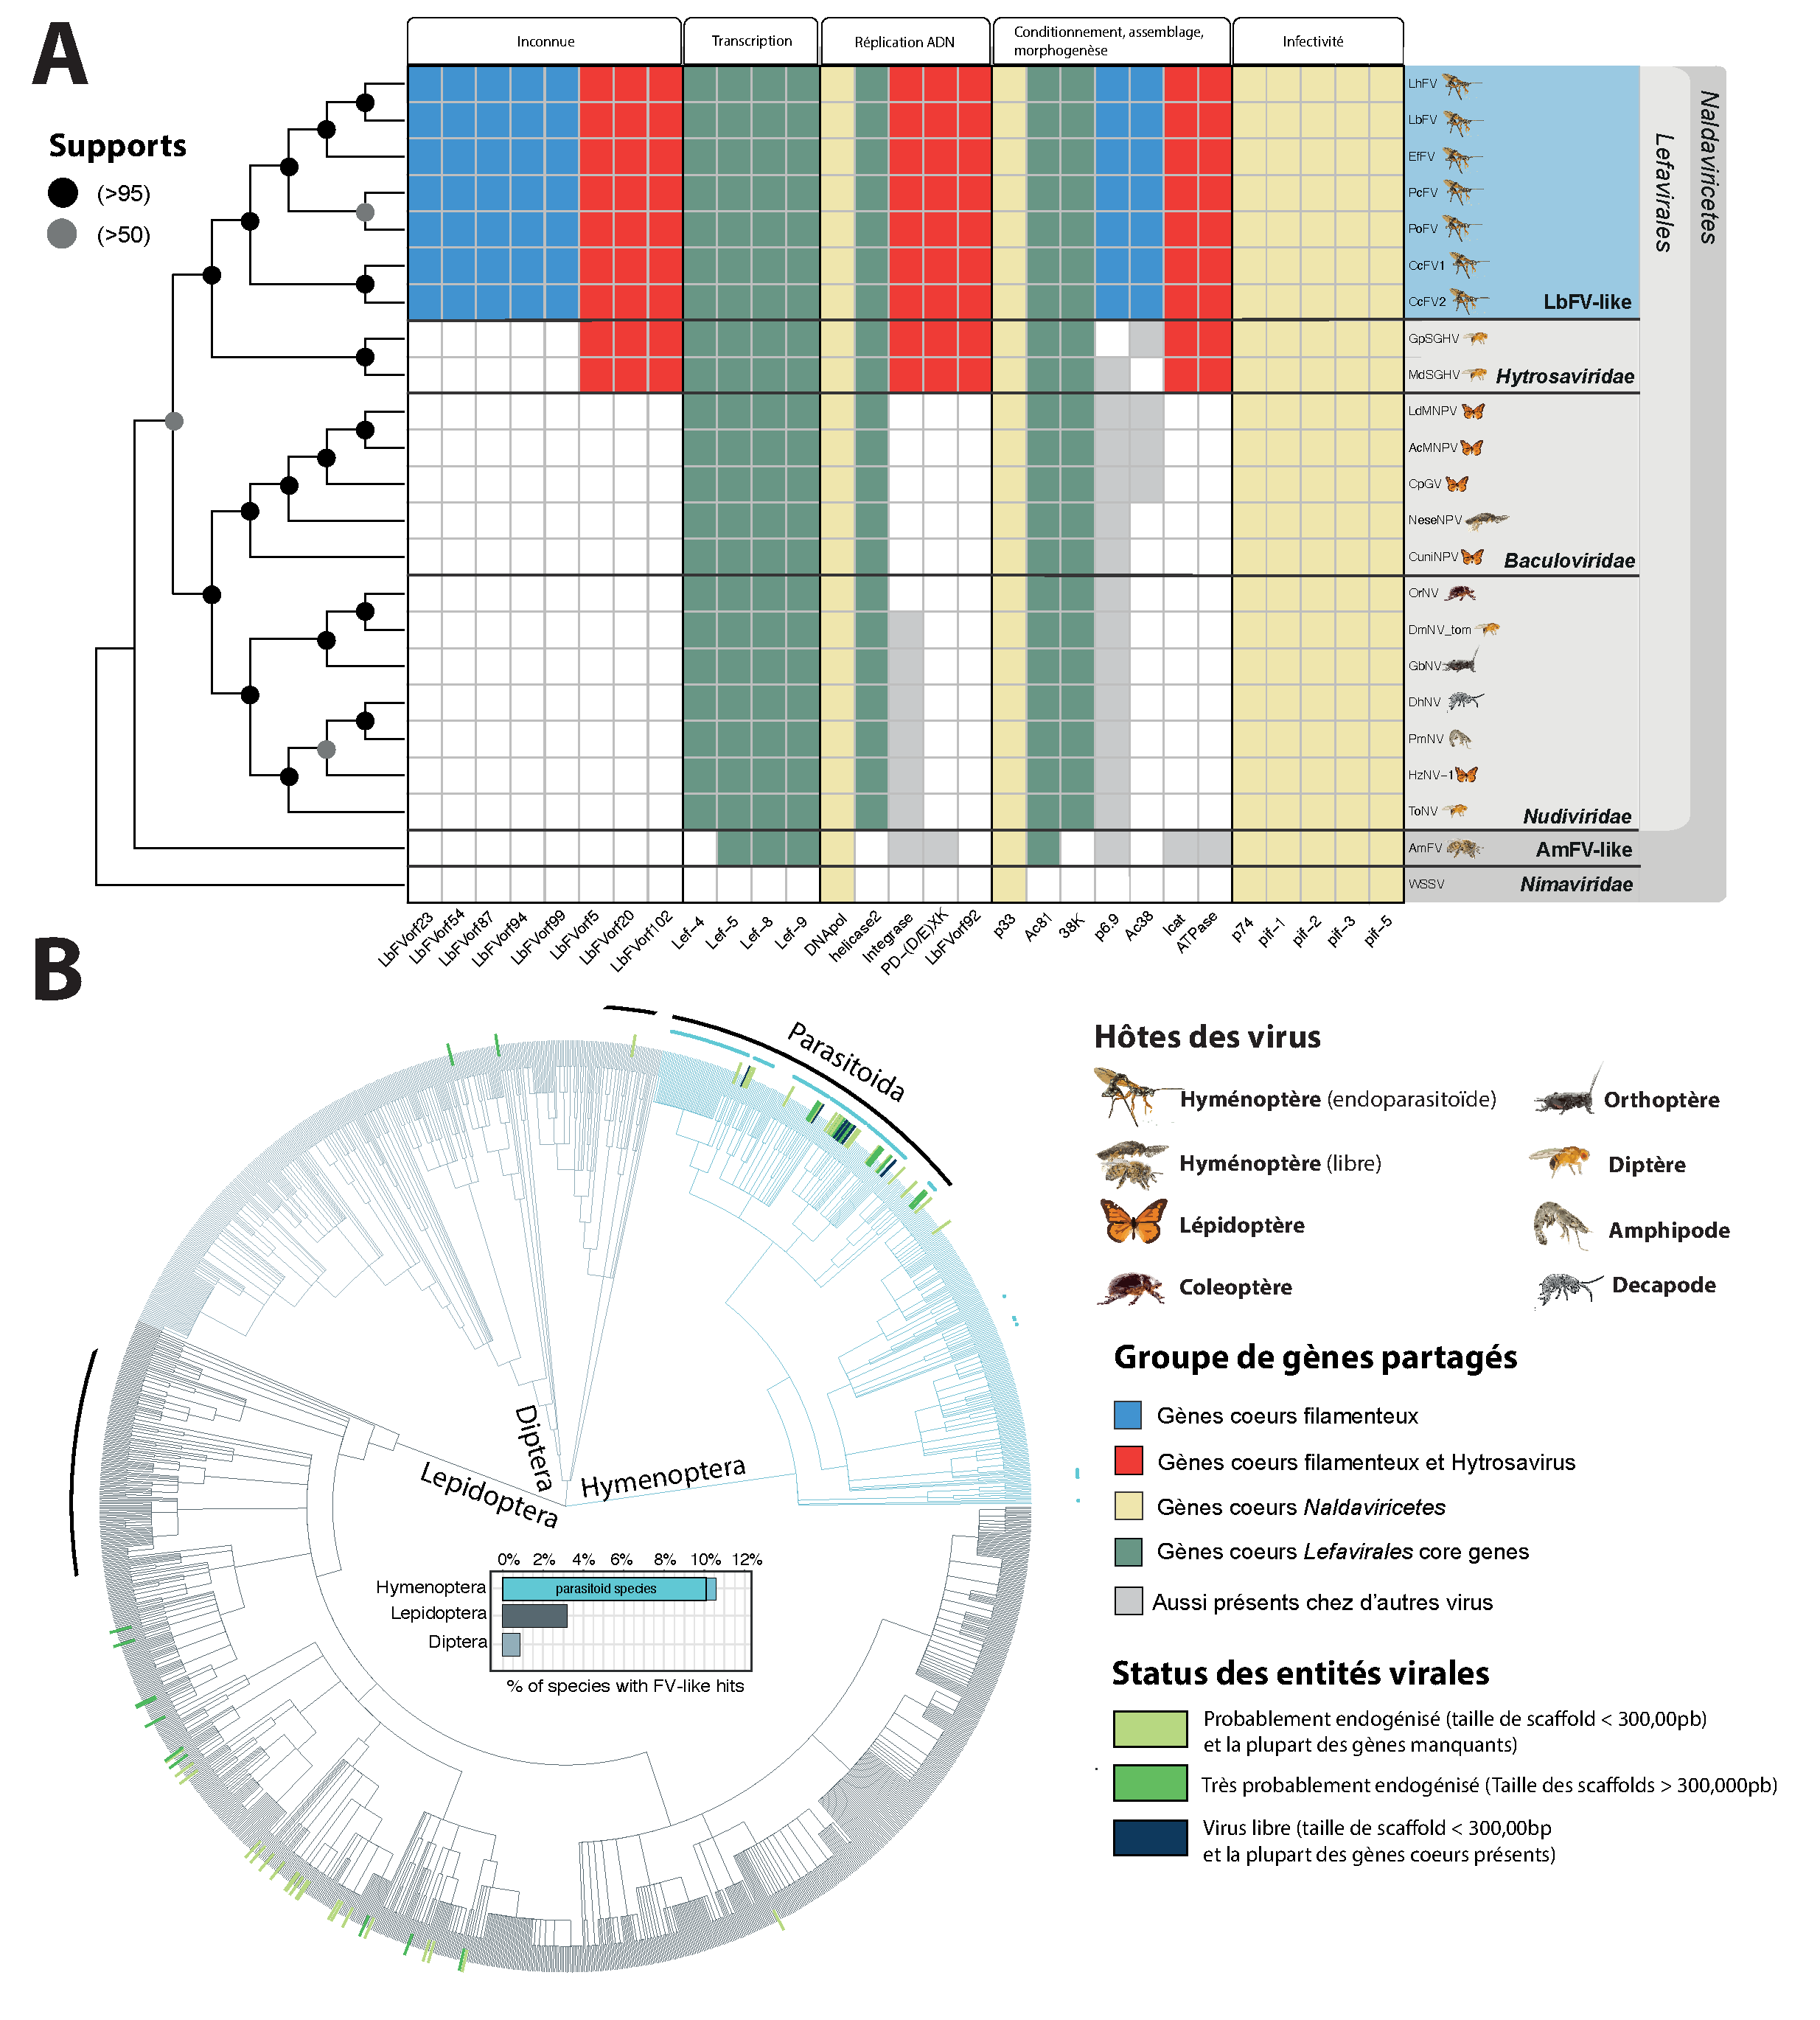
\includegraphics[width=\linewidth,height=\textheight,keepaspectratio]{PhD-master/figures/Resume_figure_papier2.pdf}
\caption[Paper2:Figures principales récapitulatives du chapitre2]{\footnotesize\textbf{Figures principales récapitulatives du chapitre2}. \textbf{A} - Heatmap représentant le contenu en gènes principaux des virus filamenteux par rapport aux autres espèces virales à ADNdb de la classe des \textit{Naldaviricetes}. Un cladogramme phylogénique est reporté sur la droite. Les lignes représentent les espèces virales, et les colonnes représentent les gènes distribués en fonction de leurs fonctions potentielles. Les cellules colorées représentent la présence du gène dans les génomes viraux (jaune pâle = gènes cœurs partagés par les espèces \textit{Naldaviricetes}, vert = gènes cœurs partagés par les espèces \textit{Lefavirales}, rouge = gènes cœurs filamenteux et hytrosavirus, bleu = gènes cœurs filamenteux et gris = présence dans d'autres génomes viraux). Les ordres des hôtes des virus sont affichés à côté du nom des virus. \textbf{B} - L'arbre phylogénétique circulaire montre les relations évolutives entre trois ordres d'insectes. La couleur des branches fait référence aux ordres d'insectes : bleu = Hyménoptères, gris clair = Diptères, gris foncé = Lépidoptères. Chaque tiret de couleur le long des feuilles de l'arbre représente le statut des éléments filamenteux (vert = FV endogène, bleu foncé = FV exogène vivant librement). Le cladogramme phylogénétique a été reconstruit sur la base du niveau NCBI taxonomique de tous les génomes étudiés dans cette analyse en utilisant la fonction NCBITaxa ete3 en python. La distribution du pourcentage d'espèces ayant des séquences de type FV dans chaque ordre d'insecte analysé est affichée dans le cladogramme à l'intérieur de la phylogénie.}
\label{figure:Resume_figure_papier2}
\end{figure}


Une propriété importante de ces virus est qu'ils semblent se répliquer uniquement chez des Hyménoptères parasitoïdes. En effet, tous les virus filamenteux dépistés jusqu'à présent sont hébergés par des espèces de guêpes endoparasitoïdes (\figurename{\ref{figure:Resume_figure_papier2}}-A). Néanmoins, nous ne pouvons pas exclure complètement le biais inhérent aux sujets de recherche de nos deux équipes, qui se sont principalement concentrées sur les Hyménoptères endoparasitoïdes. Aussi, j'ai mené une exploration systématique des assemblages de génomes obtenus pour 1576 espèces incluant des Diptères, Lépidoptères et Hyménoptères. Ce travail a révélé la présence de scaffolds appartenant probablement à des virus "libres" chez quelques Hyménoptères, mais aucun chez les Diptères ou les Lépidoptères. (\figurename{\ref{figure:Resume_figure_papier2}}-B). De plus, nous retrouvons une plus grande proportion d'EVEs filamenteux à l'intérieur de génome d'Hyménoptères par rapport aux deux autres ordres (\figurename{\ref{figure:Resume_figure_papier2}}-B). Malgré tout, nous parvenons également à observer en plus faible fréquence des EVEs filamenteux dans les génomes de  Diptères et Lépidoptères, ce qui suggère soit que des transferts puissent être médiés par les parasitoïdes vers leurs hôtes (\figurename{\ref{figure:Resume_figure_papier2}}-B), soit que des virus filamenteux se répliquent également chez ces espèces. De plus, un patron très marqué est apparu au sein des Hymenoptères. En effet, l'écrasante majorité des insertions virales détectées au sein de cet ordre concernait des Hyménoptères endoparasitoïdes (36/87), mais aucun ecto-parasitoïde (0/29) et seulement quelques espèces libres (4/210).\\

Aussi, le mode de vie des parasitoïdes, en particulier endo, pourrait représenter une niche écologique favorisant le maintien et la propagation de ces virus au sein des populations de guêpes. En effet, le style de vie endoparasitoïde pourrait faciliter la transmission de virus de manière verticale de la mère à la progéniture \citep{martinez_additional_2016}, dans la mesure où les femelles endoparasitoïdes injectent fréquemment des "fluides" dans leur hôte. De plus, ce mode de vie pourrait faciliter la transmission horizontale en condition de superparasitisme (partage d'un hôte par différents individus de la même espèce)\citep{varaldi_infectious_2003,coffman_viral_2022,stasiak_characteristics_2005}. De ce point de vue, la question qui reste complètement ouverte est de savoir si la manipulation du comportement est une caractéristique généralisée à tous les Filamentoviridae ou non. À ce propos, parmi 20 gènes de LbFV potentiellement impliqués dans la manipulation du comportement chez \textit{L.boulardi} \citep{varaldi_deciphering_2018}, 2 gènes font partie des 5 gènes cœurs spécifiques de la famille des Filamentoviridae. Ceci suggère que ces gènes pourraient être impliqués dans la modification comportementale de tous les Filamentoviridae. Il est clair cependant que des données phénotypiques supplémentaires et des essais fonctionnels avec d'autres guêpes infectées par des virus filamenteux seront nécessaires pour évaluer cette hypothèse.\\

En conclusion, ces résultats suggèrent que les virus filamenteux constituent une nouvelle famille préférentiellement associée au style de vie parasitoïde et distincte des \textit{Hytrosaviridae} et nous permettent de proposer les Filamentoviridae comme quatrième famille de virus dans l'ordre des \textit{Lefavirales}, rejoignant les familles \textit{Hytrosaviridae}, \textit{Nudiviridae} et \textit{Baculoviridae}. Des recherches supplémentaires sont nécessaires pour étudier la relation entre ces virus et leurs hôtes parasitoïdes et pour acquérir une connaissance plus approfondie du rôle des virus filamenteux dans les interactions parasitoïdes-virus. \\

Ces travaux complets en anglais sont disponibles dans la deuxième section du chapitre \hyperref[sec:chap2]{Études}. 


    \thispagestyle{empty}
    \chapter{Origine Crétacéenne de la domestication virale chez les guêpes parasitoïdes Eucoilini}

Dans le chapitre précédent, la famille virale des Filamentoviridae a été présentée. Depuis les années 1970, des virus ayant une forme filamenteuse ont été identifiées chez plusieurs espèces de guêpes endoparasitoïdes. D'après nos travaux, ces virus font partie d'une nouvelle famille virale, les Filamentoviridae, et semblent adaptés de manière spécifique au mode de vie endoparasitoïde dont elles ont probablement exploité les particularités écologiques au cours de leur évolution. Le premier virus filamenteux à avoir été caractérisé au niveau moléculaire infecte le parasitoïde de \textit{Drosophile} \citep{lepetit_genome_2017}  \textit{Leptopilina boulardi}. Ce virus, surnommé Leptopilina boulardi filamentous virus (LbFV), a un effet sur le comportement de ponte des guêpes. En effet, contrairement aux femelles non infectées, les femelles infectées par ce virus acceptent de pondre leurs œufs chez des hôtes déjà parasités \citep{varaldi_infectious_2003,varaldi_artifical_2006}. Cette induction du "superparasitisme" permet la transmission horizontale du virus, augmentant ainsi la valeur adaptative du virus au détriment des guêpes \citep{gandon_superparasitism_2006}. De plus, ce virus est principalement transmis verticalement de la mère à la progéniture \citep{martinez_additional_2016}, ce qui a pu faciliter des échanges fortuits de matériel génétique entre le virus et les guêpes sur le long terme. Dans ce sens, des recherches récentes suggèrent que le génome entier d'un virus ancestral apparenté a été endogénisé chez l'ancêtre commun des guêpes appartenant au genre \textit{Leptopilina} (Di Giovanni et al., 2020). Aujourd'hui, 13 gènes filamenteux (EVEs) sont présents chez tous les individus de ce genre (Di Giovanni et al., 2020). Comme chez d'autres espèces de guêpes parasitoïdes qui ont domestiqué des virus  \citep{bezier_polydnaviruses_2009,volkoff_analysis_2010,pichon_recurrent_2015,burke_common_2019}, ces gènes filamenteux endogènes ont été domestiqués et sont utilisés par les guêpes femelles pour délivrer des facteurs de virulence, qui sont nécessaires pour protéger leurs œufs du système immunitaire de l'hôte \citep{colinet_convergent_2007,di_giovanni_behavior-manipulating_2020}. Plus précisément, dans ce système, une \textit{ADN polymérase} virale (ORF58) amplifie de manière temporaire une partie des EVEs (10/13) au moment où les VLPs sont formées. L'amplification génomique se traduit par une augmentation de la transcription de ces mêmes gènes. \\

Plusieurs de ces gènes amplifiés ont des rôles connus chez des virus "libres" : dans la transcription (\textit{lef-4}, \textit{lef-8} et \textit{lef-9}), dans l'enveloppement des protéines de virulence (\textit{ac81}) \citep{ dong_autographa_2016} et la formation de membranes lipidiques (\textit{lcat}) \citep{saeedi_review_2015}. Les "virus-like particles" (VLPs) sont des structures comparables à des liposomes. Elles sont en effet constituées d'une membrane lipidique contenant des facteurs de virulence sous la forme de protéines codées par les guêpes. Une fois entièrement assemblées, ces particules sont injectées avec l'œuf pendant l'oviposition et leur contenu est libéré au sein des cellules immunitaires de l'hôte, les hémocytes \citep{rizki_parasitoid_1990,colinet_convergent_2007}. Une fois à l'intérieur des cellules, les protéines de virulence génèrent des changements morphologiques importants qui empêchent les cellules d'initier une réponse immunitaire efficace contre l'œuf de parasitoïde \citep{colinet_convergent_2007}. En outre, nous savons que ces EVEs proviennent très probablement d'un seul événement d'endogénisation puisque les phylogénies des 13 EVEs sont identiques et congruentes avec celle des guêpes, et parce que nous détectons des conservations de blocs synténiques entre les génomes de guêpes. Cependant, aucune estimation de l'âge de cet évènement, ni de la diversité d'espèces concernée ne sont actuellement disponibles. Nous savons néanmoins que l'espèce éloignée du genre \textit{Ganaspis} ne présente aucune preuve d'endogénisation (Di Giovanni et al., 2020).\\

Afin d'étudier la diversité des guêpes impliquées dans cet évènement, nous avons donc recherché par PCR la présence de l'ORF le plus conservé (ORF96) chez 41 spécimens de Figitidae. En nous appuyant sur la phylogénie de \citep{blaimer_comprehensive_2020}, nous avons complété par l'analyse de trois espèces appartenant à cette tribu, \textit{Rhoptromeris}, \textit{Thrichoplasta}, \textit{Trybliographa}, et \textit{Leptolamina}, dont nous avons séquencé le génome.\\

Nous avons ensuite cherché de manière systématique des homologies de séquences avec tous les ORFs prédits de la famille des Filamentoviridae décrite au (\hyperref[sec:chap2]{chapitre 2}). À l'exception de l'espèce la plus basale du groupe "\textit{Leptolamina}", les six génomes d'Eucoilini présentaient des homologies de séquence élevées avec chacun des 13 EVEs signalés précédemment (\figurename{\ref{figure:Cynipoidea_EVE_heatmap_french}}). Les phylogénies de ces gènes (Type 1 sur la  \figurename{\ref{figure:Type_EVE_phylogenies_french}}) et la conservation de la synténie pour certains d'entre eux étaient cohérents avec un scénario d'endogénisation ancestrale chez l'ancêtre commun des 6 espèces d'Eucoilini. \\


\begin{figure}[!htpbt]
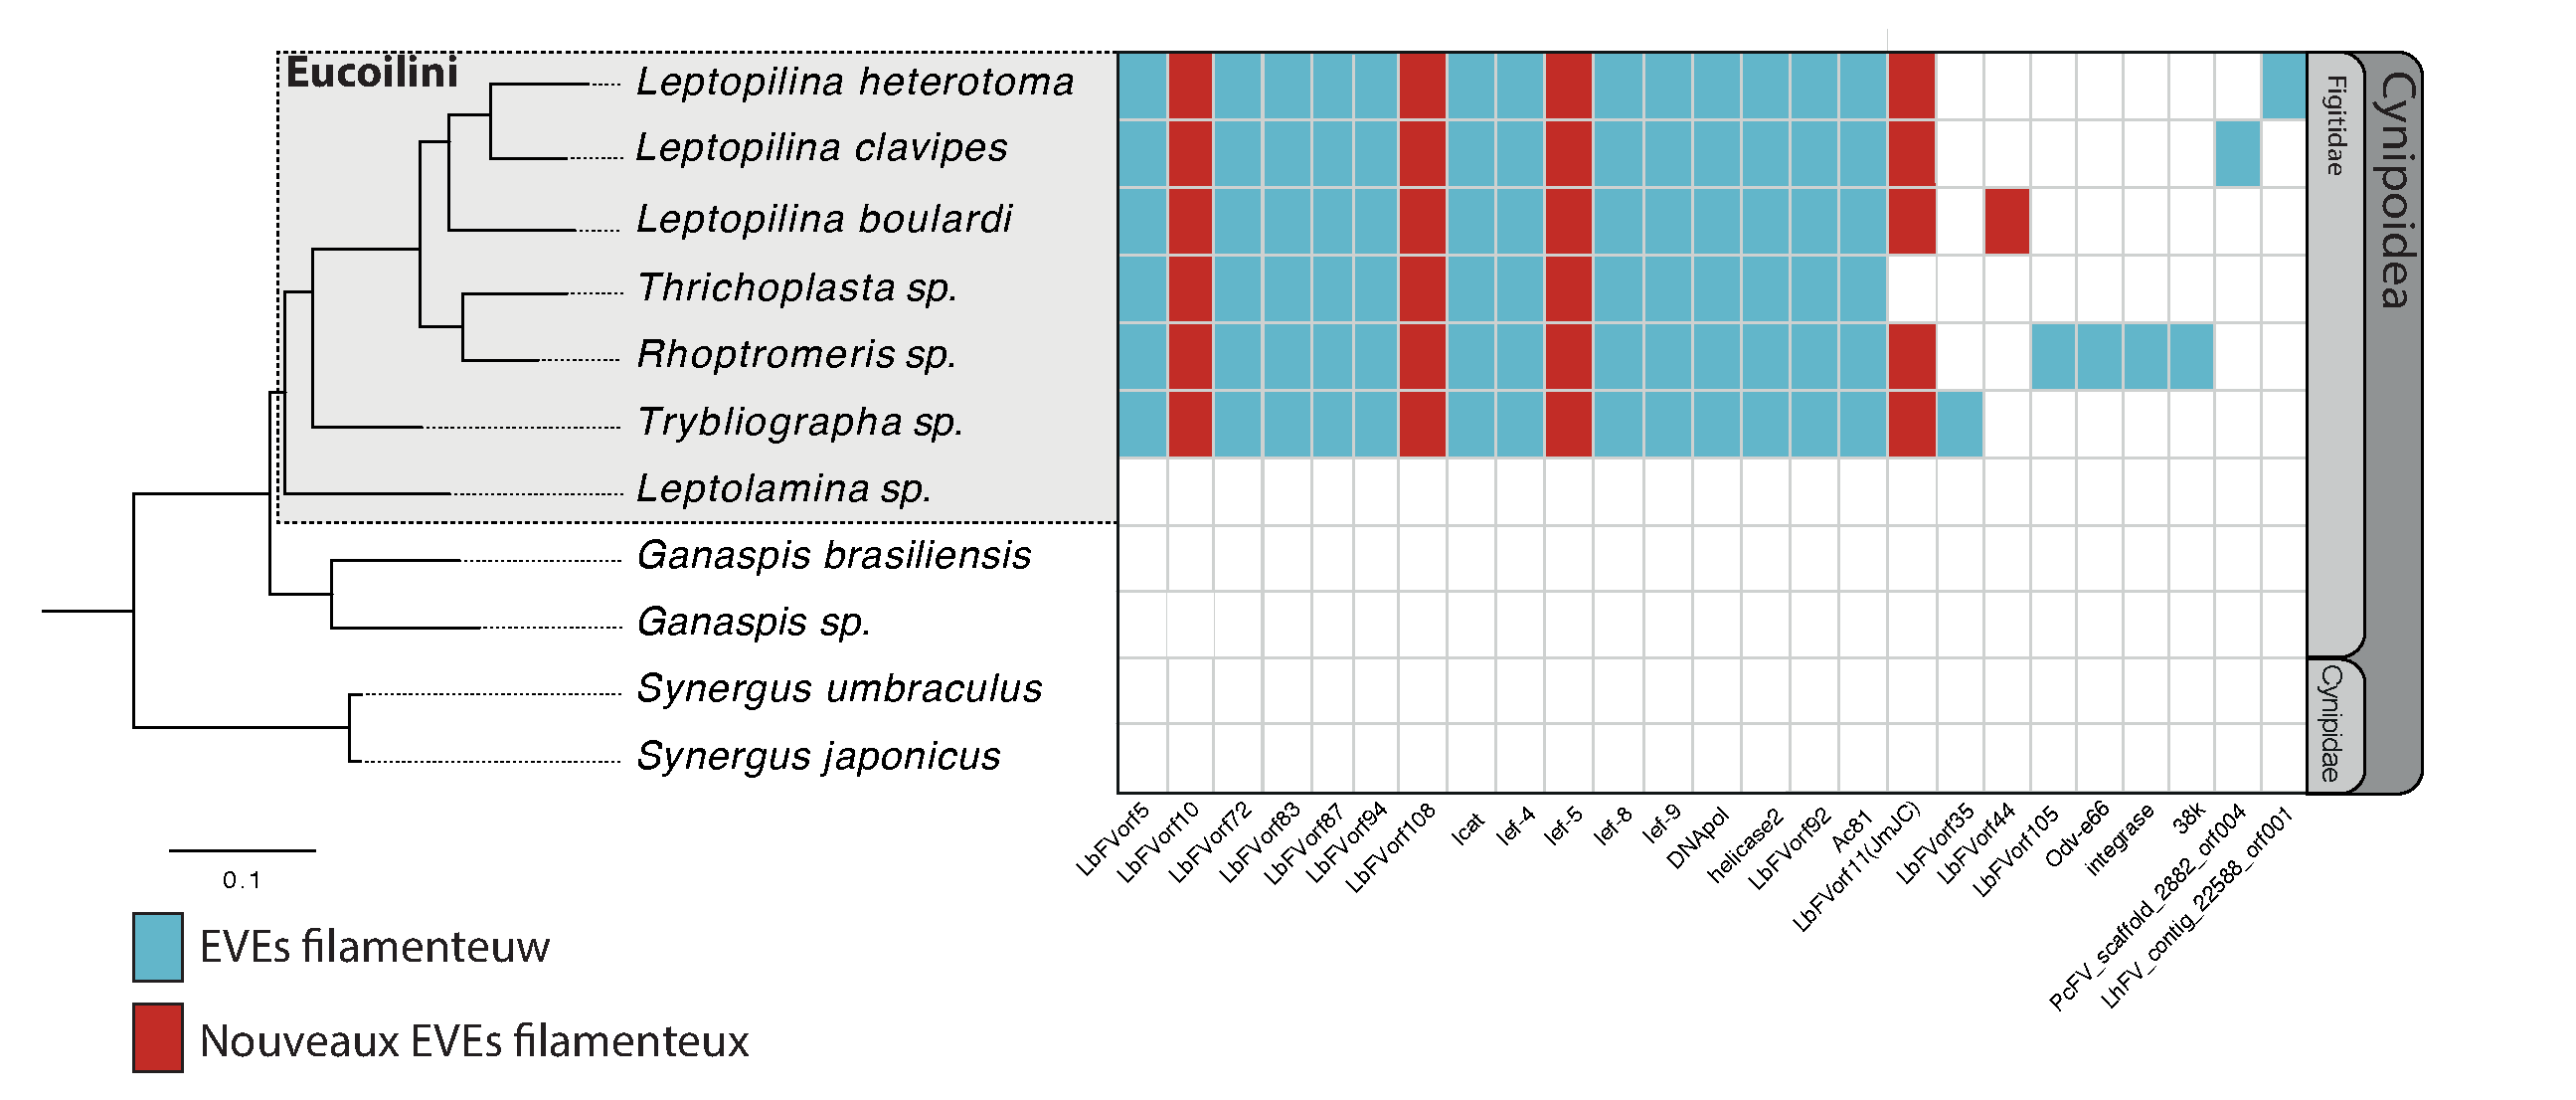
\includegraphics[width=\linewidth,height=\textheight,keepaspectratio]{PhD-master/figures/Cynipoidea_EVE_heatmap_french.pdf}\centering
\caption[Paper3:Distribution des EVE filamenteux parmi les espèces de Cynipoidea]{\textbf{Distribution des EVE filamenteux parmi les espèces de Cynipoidea}. La phylogénie des Cynipoidea a été estimée à l'aide de 1 000 gènes BUSCO. Chaque ligne représente une espèce de Cynipoidea, tandis que chaque colonne représente un EVE filamenteux.
Les cases bleues indiquent la présence d'EVE dans un génome, tandis que les cases blanches indiquent son absence. Les cases rouges indiquent les EVEs nouvellement assignés provenant du même évènement ancestral que dans \cite{di_giovanni_behavior-manipulating_2020}.}
\label{figure:Cynipoidea_EVE_heatmap_french}
\end{figure}


\begin{figure}[!htpbt]
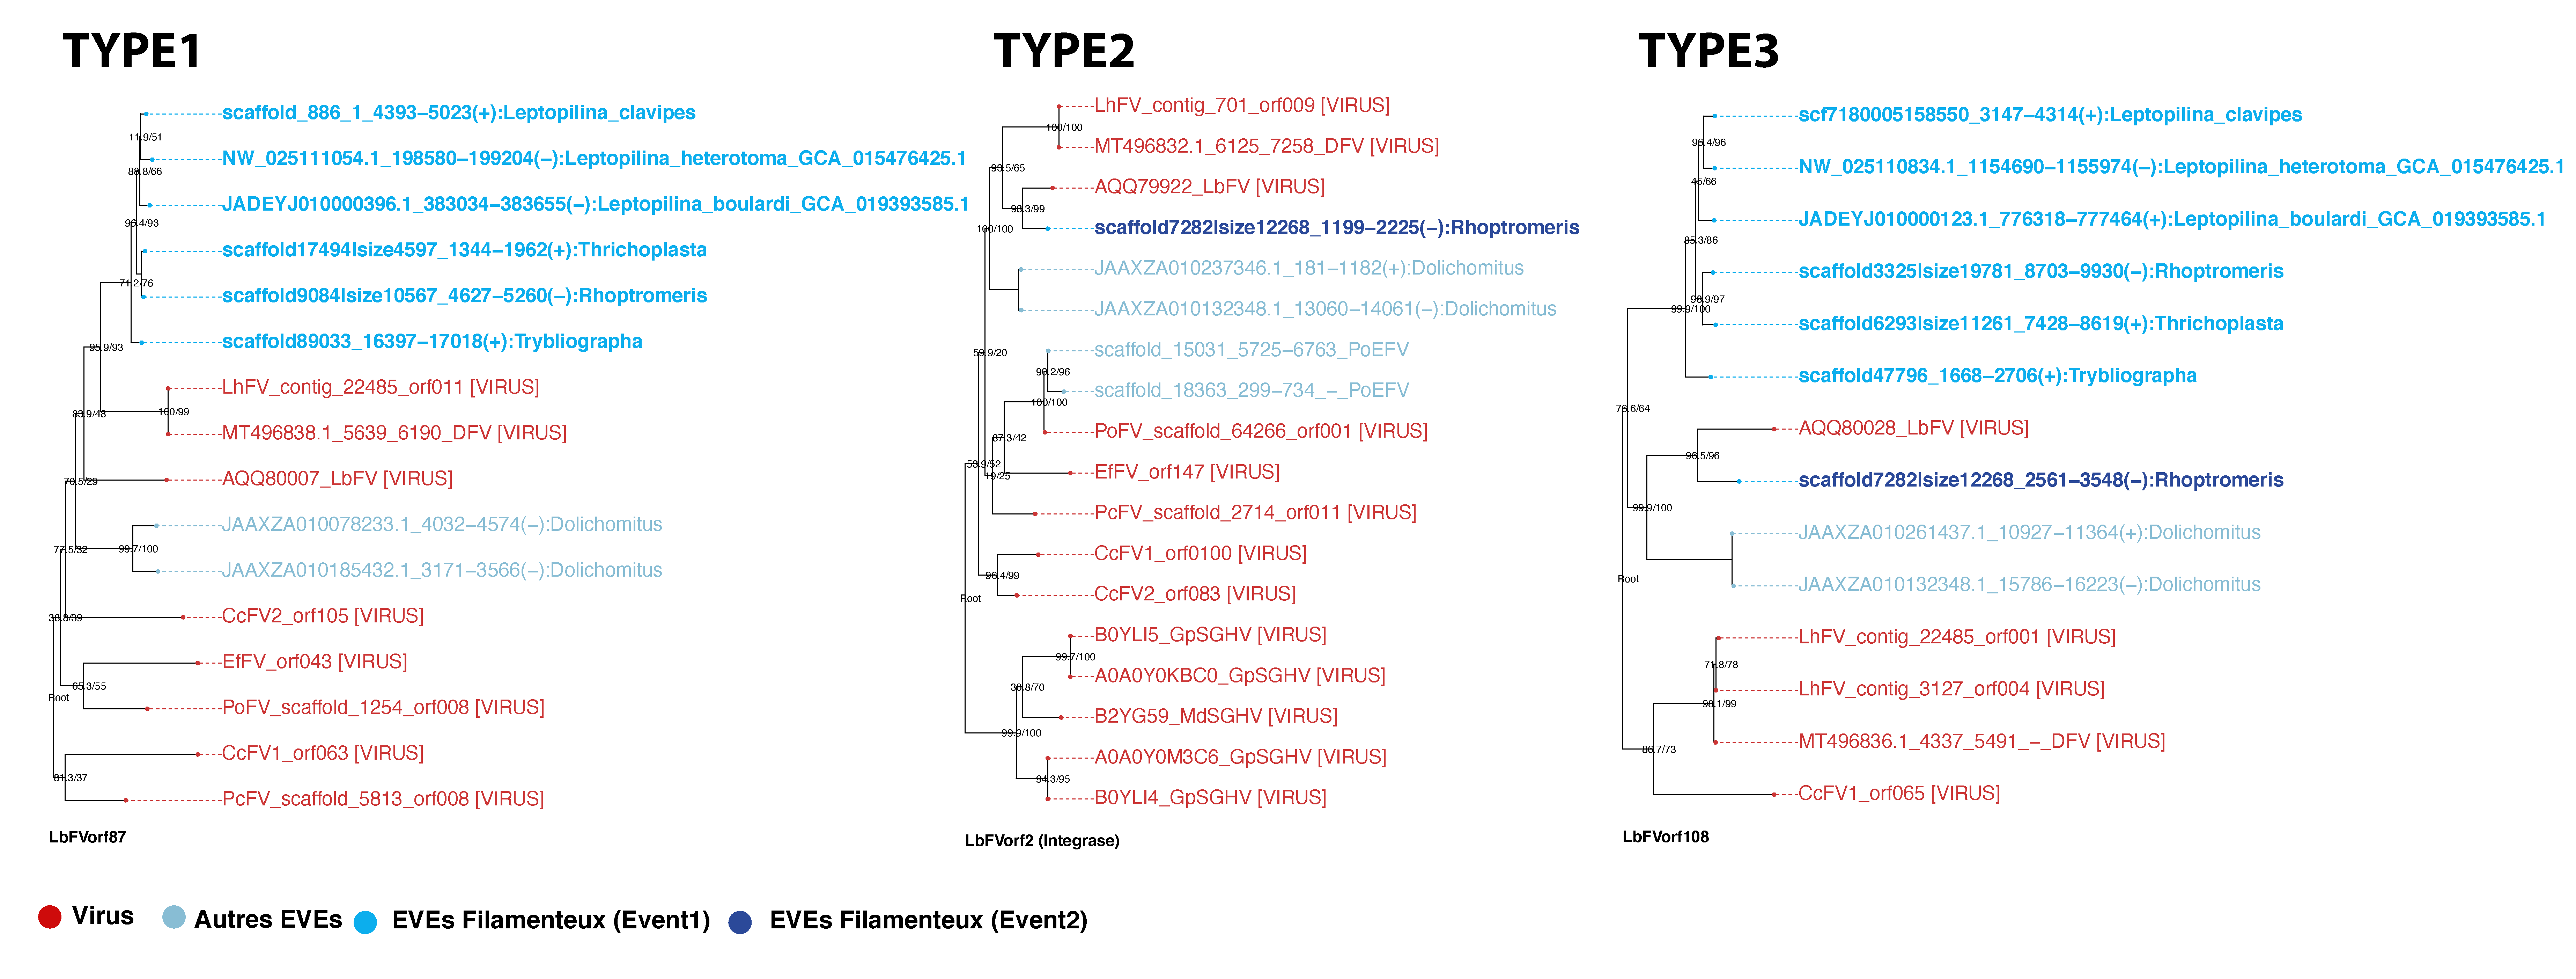
\includegraphics[width=\linewidth,height=\textheight,keepaspectratio]{PhD-master/figures/Type_EVE_phylogenies_french.pdf}\centering
\caption[Paper3:Type de phylogenies d'EVEs filamenteux chez les Eucoilini]{\textbf{Exemple de phylogénies d'EVEs filamenteux observées}. Le type1 correspond à un événement d'endogénisation unique qui s'est produit chez l'ancêtre de la majeure partie des Eucoilini et impliquant un donneur proche de LhFV. Le type2 suggère un autre événement indépendant qui s'est produit dans la branche \textit{Rhoptromeris} et impliquant un donneur proche de LbFV. Les phylogénies de type3 suggèrent que les deux événements se sont produits pour ce gène}.
\label{figure:Type_EVE_phylogenies_french}
\end{figure}

De plus, l'analyse a révélé la présence de 5 gènes supplémentaires (non identifiés par \cite{di_giovanni_behavior-manipulating_2020}) issus du même événement d'endogénisation. Comme attendu pour des gènes impliqués dans la formation de structures liées à la fitness des guêpes comme les VLPs, chacun de ces gènes présentait un régime de sélection purifiant. Bien que ces résultats indiquent que ces gènes sont étroitement associés à la fitness de ces guêpes, nous manquions de connaissances sur leurs conséquences phénotypiques  chez les espèces d'Eucoilini en dehors des \textit{Leptopilina}. Au cours de sa thèse de doctorat soutenue en 1999 à l'Université de Rennes, Nabila Kacem Haddj El Mrabet a décrit la présence de VLPs dans la glande à venin de \textit{Trybliographa rapae}(\figurename{\ref{figure:Microscopy_Lboulardi_Trybliographa_resume}}). Ces résultats, obtenus sur l'espèce la plus basale du groupe concerné par l'évènement d'endogénisation, permettent d'envisager que l'ensemble des espèces, depuis les \textit{Leptopilina} et jusqu'aux \textit{Trybliographa}, produisent effectivement des VLPs grâce aux gènes filamenteux domestiqués.\\

\begin{figure}[H]
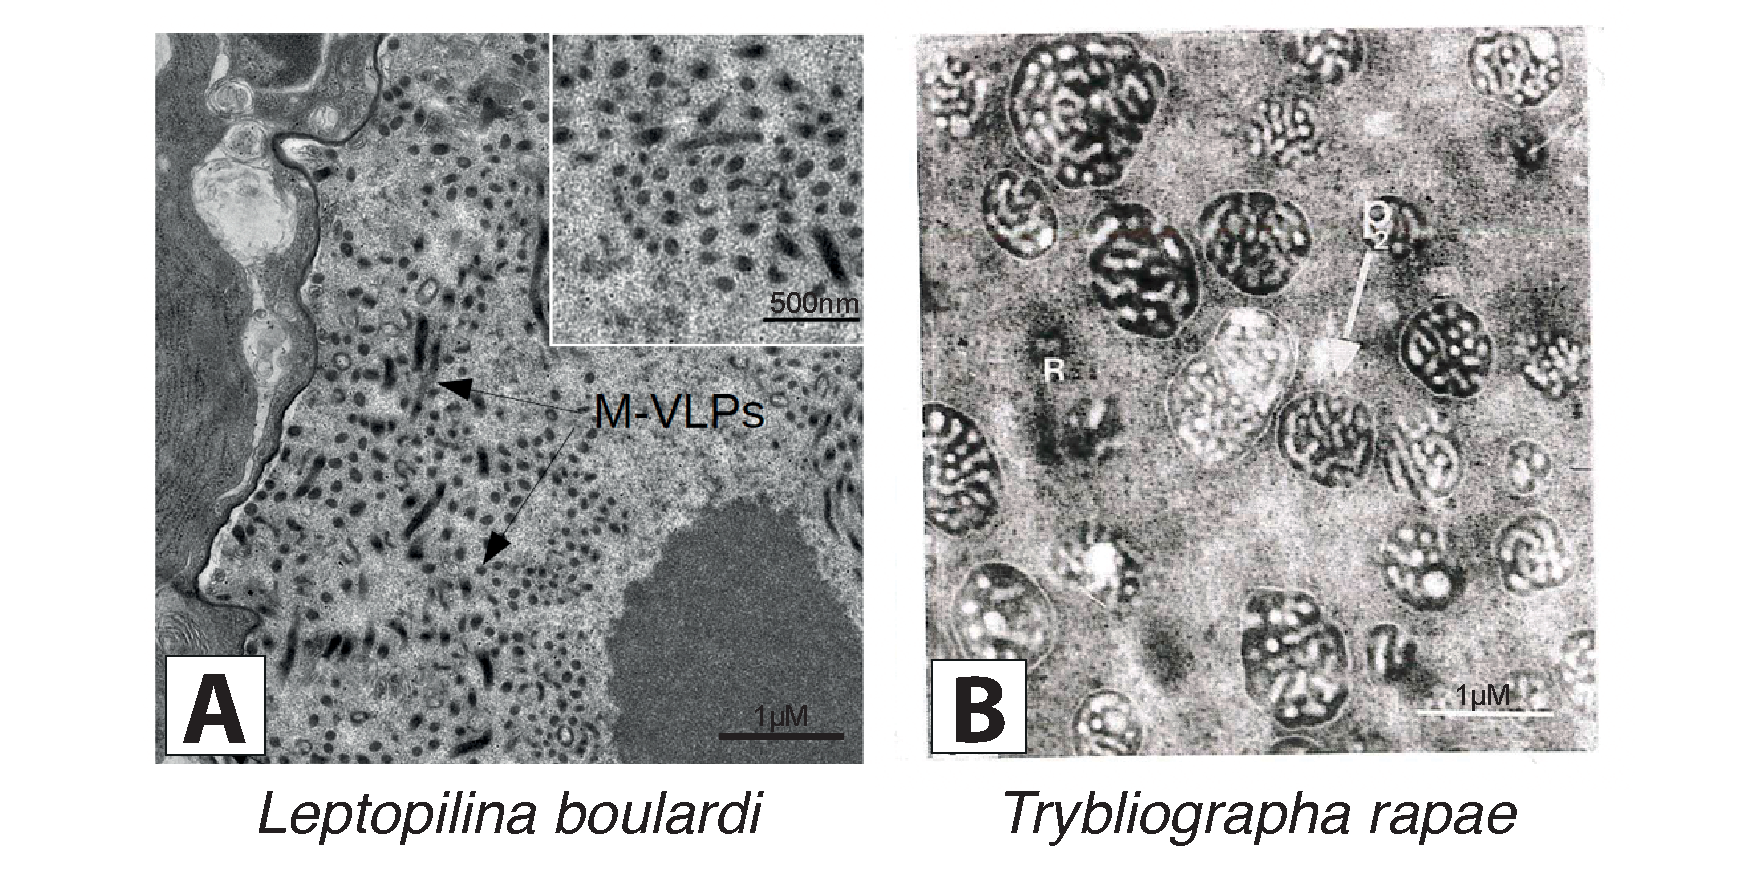
\includegraphics[width=\linewidth,height=\textheight,keepaspectratio]{PhD-master/figures/Microscopy_Lboulardi_Trybliographa_resume.pdf}\centering
\caption[Paper3:[Microscopie électronique des VLPs chez \textit{L.boulardi} et \textit{T.rapae}]{Photos de microscopies électroniques des VLPs produits dans la glande à venin de \textit{Lepoptilina boulardi} (A) et \textit{Trybliographa rapae} (B) provenant respectivement de \cite{di_giovanni_behavior-manipulating_2020} et D.Poinçot et K.Haddj E PhD 1999.}
\label{figure:Microscopy_Lboulardi_Trybliographa_resume}
\end{figure}

En plus de cet évènement majeur d'endogénisation virale, nous avons également découvert une endogénisation plus récente chez \textit{Rhoptromeris}. Cet événement implique 9 EVEs, dont certains sont pseudogénisés et d'autres sont encore intacts et dont les phylogénies représentent des topologies de type 2 et 3 (\figurename{\ref{figure:Type_EVE_phylogenies_french}}). De façon remarquable, l'un des 18 gènes identifiés dans l'événement initial semble avoir été remplacé par un gène homologue provenant de ce deuxième événement chez \textit{Rhoptromeris}. \\

Nous avons observé des similitudes structurelles entre ce gène et une protéine de Hantavirus qui remplit une fonction impliquée dans les mécanismes d'entrée virale dans les cellules hôtes \citep{guardado-calvo_surface_2021}. Le remplacement de ce gène chez cette espèce pourrait avoir amélioré l'efficacité avec laquelle les VLPs produits par \textit{Rhoptromeris} pénètrent dans les cellules immunitaires de leurs hôtes Diptères de la famille des Chloropidae.\\

Pris dans leur ensemble, ces résultats indiquent qu'un événement d'endogénisation s'est donc produit chez l'ancêtre commun de ces 6 espèces d'Eucoilini, il y a environ 75 millions d'années, selon une estimation récente de l'age de ce nœud dans la phylogénie des Cynipoidea \citep{blaimer_comprehensive_2020}. La période estimée de cet événement coïncide avec la diversification des Diptères Schizophora qui sont les hôtes de ces guêpes parasitoïdes \citep{wiegmann_episodic_2011} (\figurename{\ref{figure:Schizophora_Eucoilini_virus_phylogeny_french}}). Nous pouvons donc émettre l'hypothèse que la production de VLPs, aurait permis à ces espèces de coloniser et de s'adapter à de nombreux hôtes Schizophora au cours de la radiation du groupe. \\

\begin{figure}[!htpbt]
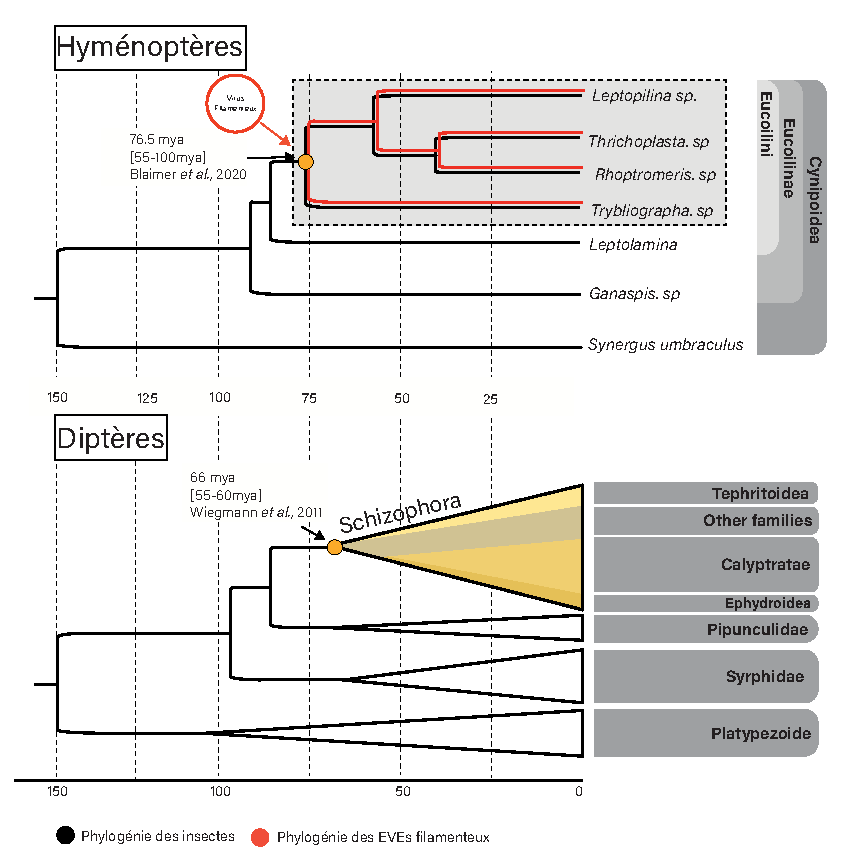
\includegraphics[width=\linewidth,height=\textheight,keepaspectratio]{PhD-master/figures/Schizophora_cynipids_virus_phylogeny_french.pdf}\centering
\caption[Paper3:Arbres phylogénétiques des Eucoilini et des EVEs filamenteux]{\textbf{Arbres phylogénétiques des hôtes et des EVEs filamenteux}. Les branches noires correspondent aux branches des Hyménoptères (en haut) ou des Diptères (en bas), tandis que les branches rouges correspondent aux branches des EVEs filamenteux. Les arbres ont été reconstruits en utilisant les sources suivantes :\citep{blaimer_comprehensive_2020} pour les données sur les Hyménoptères, et \citep{wiegmann_episodic_2011} pour la phylogénie des Diptères. La phylogénie des virus filamenteux endogènes a été déduite de la concaténation des 16 éléments viraux filamenteux endogènes partagés par tous les Eucoilini).}
\label{figure:Schizophora_Eucoilini_virus_phylogeny_french}
\end{figure}

\newpage
Enfin, en utilisant les données fournies par l'événement d'endogénisation chez les Eucoilini (impliquant un virus filamenteux permettant la formation de VLPs) et celui impliquant les guêpes du complexe des Microgastroïde (impliquant un nudivirus et permettant la production de  polydnavirus), nous avons pu calibrer la phylogénie des \textit{Naldaviricetes}, à laquelle appartiennent les deux virus donneurs. Les inférences estiment que les Filamentoviridae seraient apparus il y a 250 à 350 millions d'années, ce qui coïncide avec le moment où les Hyménoptères ont commencé à se diversifier entre le Carbonifère et le Trias (239-329 millions d'années) \citep{peters_evolutionary_2017}. Les Filamentoviridae sont des virus qui semblent être spécifiques des Hyménoptères, et selon toute vraisemblance plus spécifiquement aux guêpes endoparasitoïdes. Plus spécifiquement, les lignées de guêpes parasitoïdes les plus diverses (c'est-à-dire Ceraphronoidea, Ichneumonoidea et Proctotrupomorpha) ont connu une extraordinaire radiation entre 195 et 265 millions d'années \citep{peters_evolutionary_2017}. Par conséquent, nous pourrions spéculer que ces virus seraient apparus au moment de la diversification des Hyménoptères avant de se specialiser sur les lignées de guêpes endoparasitoïdes. La longue histoire évolutive commune a ensuite entrainé l'endogénisation accidentelles de virus dans un processus dynamique, comme nous avons pu l'observer chez  \textit{Rhoptromeris}. Néanmoins, ces données montrent qu'il est difficile de remplacer une machinerie virale complète si les gènes nouvellement acquis ont des fonctions redondantes au système déjà en place, mais concernerait plutôt le remplacement de quelques gènes dans un système déjà établi.  Le seul exemple supplémentaire de remplacement d'une machinerie virale entière serait chez \textit{V. canescens}, où un ichnovirus (polydnavirus) aurait été remplacé par un nudivirus (VLPs) \citep{pichon_recurrent_2015}. Cependant, l'analyse faite dans le (\hyperref[sec:chap1]{chapitre 1}) (qui incluait \textit{V. canescens}), n'a pas permis de confirmer ce remplacement.\\

Ces travaux complets en anglais sont disponibles dans la troisième section du chapitre \hyperref[sec:chap3]{Études}. 



    
    \part{Discussion générale}
    \label{part:discussion}
    \thispagestyle{empty}
\chapter{Discussion générale}
{\hypersetup{linkcolor=GREYDARK}\minitoc}
\label{chap:discuss-general}


\section{Résumé des principaux résultats}

Au cours de mes travaux de thèses, nous avons vu que tout le long de l'histoire évolutive des espèces, l'intégration accidentelle d'éléments viraux dans le génome eucaryote peut se produire \citep{katzourakis_endogenous_2010}. Ces éléments peuvent parfois conférer aux génomes receveurs des avantages évolutifs majeurs : on parle alors de domestication virale. Par exemple, chez certaines guêpes endoparasitoïdes (dont les stades immatures se développent à l'intérieur de leurs hôtes), la propriété fusogènique des virus a été domestiquée à plusieurs reprises suite à des intégrations virales ancestrales de virus dsDNA. Ces gènes viraux endogénisés sont utilisés par les guêpes femelles comme un outil pour injecter des facteurs de virulence, essentiels au succès du développement de leur progéniture \citep{drezen_endogenous_2017}. Comme tous les cas connus de domestication virale impliquent des guêpes endoparasitoïdes \citep{bezier_polydnaviruses_2009,volkoff_analysis_2010,pichon_recurrent_2015,burke_common_2019,di_giovanni_behavior-manipulating_2020}, nous avons au début de ma thèse émis l'hypothèse que ce mode de vie (favorisant une interaction étroite entre les individus) pouvait favoriser l'endogénisation et la domestication de virus. Ainsi, en analysant la composition génomique de 124 génomes d'Hyménoptères répartis dans la diversité des Hyménoptères et incluant des espèces libres, ecto et endoparasitoïdes, nous avons testé cette hypothèse dans le \hyperref[sec:chap1]{chapitre 1}. Notre analyse a d'abord révélé que les virus à ADN double brin étaient plus souvent endogénisés et domestiqués que prévu d'après leur abondance relative estimée dans les communautés virales infectant les insectes par rapport aux autres structures génomiques virales (ssDNA, dsRNA, ssRNA). Deuxièmement, notre analyse a révélé que l'endogénisation et la domestication des virus à ADN double brins étaient plus fréquentes dans les espèces ayant un mode de vie endoparasitoïde par rapport aux espèces ayant un mode de vie ectoparasitoïde ou libre. Ces résultats suggèrent donc que l'endoparasitoïsme a promu la domestication des virus à ADN double brins ou inversement que la domestication de ces virus a favorisé l'évolution de l'endoparasitoïsme.\\
 
Deuxièmement, dans un projet collaboratif avec l'équipe de l'IRBI de Tours, j'ai pu exploiter les données dites "exogènes" de mon premier projet pour décrire cette fois-ci plutôt de nouveaux virus infectieux présents dans des assemblages de génomes de guêpes parasitoïdes. Nous avons en particulier recherché la présence de virus à allure filamenteuse apparentés au virus retrouvé chez l'espèce parasitoïde \textit{Leptopilina boulardi}. Ce virus connu pour manipuler le comportement du parasitoïde est actuellement le seul représentant d’une probable nouvelle famille de virus à ADN. C'est ainsi qu'au cours de ce projet, nous avons pu caractériser cette nouvelle famille virale en analysant le contenu en gènes et l’histoire évolutive de 7 nouveaux génomes de virus appartenant à cette famille. Ce travail constitue ainsi la base préliminaire pour leur classification dans l'ICTV comme une nouvelle famille que nous proposons de nommer Filamentoviridae en raison de leur structure filamenteuse singulière, créant ainsi une cinquième famille de la classe \textit{Naldaviricetes} des virus à ADN double brins. Ces résultats tendent également à montrer que ces virus sont préférentiellement associés à des espèces de guêpes endoparasitoïdes dont le style de vie particulier a très probablement permis à ces virus de se transmettre efficacement entre générations.\\
 
Enfin, la dernière partie de mon doctorat consistait à étudier les EVEs dans un clade de guêpes endoparasitoïdes initialement identifié dans notre laboratoire (Di Giovanni et al., 2020). Ce clade correspond aux espèces du genre \textit{Leptopilina}, chez qui 13 gènes provenant de la famille des Filamentoviridae ont été domestiqués et participent à la production de particules virales qui protègent les œufs des guêpes du système immunitaire de leur hôte. Mes résultats indiquent qu'un événement d'endogénisation et de domestication virale s'est produit il y a environ 75 millions d'années chez l'ancêtre commun de la majorité des espèces de guêpes appartenant à la tribu des Eucoilini (contenant les \textit{Leptopilina}). L'endogénisation de ces gènes correspond à la période de diversification des hôtes de ces guêpes parasitoïdes, ce qui suggère que la domestication des gènes viraux ait pu aider les guêpes à s'adapter à leurs hôtes à cette époque. Par ailleurs, nous mettons également en évidence un nouvel évènement indépendant ayant probablement donné lieu au remplacement d'un gène provenant du premier évènement chez l'espèce \textit{Rhoptromeris}. Enfin, la caractérisation temporelle du premier événement d'endogénisation ancestral au sein des Eucoilini nous a permis de calibrer la phylogénie des Filamentoviridae. Cette calibration nous permet d'estimer que la diversification des Filamentoviridae a eu lieu, il y a environ 297 millions d'années, ce qui correspond à peu près au moment de l'apparition des Hyménoptères. Par la suite, au cours de l'évolution, ces virus se seraient ensuite préférentiellement associés aux lignées d'Hyménoptères ayant un mode de vie endoparasitoïde.\\ 

%coïnciderait à nouveaux avec l'hypothèse initiale que ces virus sont intrinsèquement liés à ce mode de vie.  \\

%Ces trois chapitres abordent plusieurs questions sur plusieurs échelles évolutives. Au-delà de la discussion de chacun de ces travaux, nous pouvons donc tenter de discuter plus largement des implications de ces résultats et ce qu'ils peuvent nous apprendre de la biologie et l'évolution des espèces endoparasitoïdes et des virus avec lesquels elles interagissent depuis des millions d'années. \\


\section{Pourquoi les phénomènes de domestication sont-ils plus fréquents chez les espèces endoparasitoïdes et impliquent préférentiellement les virus dsDNA?}

Dans le \hyperref[sec:chap1]{chapitre 1}, nous mettons en évidence que le mode de vie endoparasitoïde favorise davantage les événements d'endogénisation et de domestication des virus dsDNA que les modes de vie ectoparasitoïde ou libre. Plusieurs questions se posent à la suite de ces observations. Pourquoi ce phénomène est-il limité aux virus dsDNA ? Pourquoi le mode de vie endoparasitoïde est-il préférentiellement associé à de tels événements, et quels effets, le cas échéant, ces évènements de domestication ont-ils sur la biologie de ces espèces ?\\

\textbf{H1 - Un plus grand input en virus chez les endoparasitoïdes?}

Comme première hypothèse pour comprendre ces observations, nous pourrions imaginer que l'écologie particulière des espèces endoparasitoïdes  en interaction étroite avec leur hôte soit associée à un plus grand nombre d'opportunités d'intégrations virales accidentelles. En effet, des endoparasitoïdes peuvent être plus intensivement exposés aux virus comparé à d'autres Hyménoptères au style de vie ectoparasitoïde ou bien libre.

De multiples éléments viennent étayer cette hypothèse. Les larves endoparasitoïdes se développent par définition à l'intérieur du corps de leur hôte, et une interaction aussi étroite implique que tout individu endoparasitoïde interagira également avec les virus de son hôte. En appui à cette idée, il est intéressant de noter que la plupart des cas de domestication de virus par les  guêpes endoparasitoïdes impliquent les nudivirus. Les virus de cette famille infectent en effet les Lépidoptères qui sont les hôtes des parasitoïdes en question \citep{burke_rapid_2018,pichon_recurrent_2015,bezier_polydnaviruses_2009-1}. Un autre facteur important est la présence de virus dans les venins que les endoparasitoïdes injectent dans les hôtes au côté de leurs œufs. La présence de ces virus dans ces compartiments pourrait favoriser la propagation ultérieure des virus dans les populations de guêpes. Par exemple, en colonisant les tissus producteurs de venin (glande venimeuse ou calice, selon la biologie de l'espèce), les virus peuvent assurer une transmission pseudo-verticale efficace et ainsi se maintenir efficacement dans les populations de guêpes. De nombreux virus endoparasitoïdes bénéficient d'une telle transmission pseudo-verticale \citep{varaldi_artifical_2006,renault_cypovirus_2003,coffman_viral_2022}, dont certains ont été domestiqués par les endoparasitoïdes (ou tout du moins leurs ancêtres) (Di Giovanni et al., 2020). La présence de virus dans les venins peut également faciliter la transmission horizontale au sein des espèces en cas de superparasitisme, par exemple chez le virus filamenteux de \textit{Leptopilina boulardi} infectant des drosophiles \citep{varaldi_infectious_2003} ou bien l'entomopoxvirus chez \textit{Diachasmimorpha longicaudata} infectant des larves de mouches des fruits téphritides \citep{coffman_viral_2022}, ou bien encore un ascovirus mutualiste (DpAV4) chez plusieurs espèces du genre \textit{Diadromus} \citep{stasiak_characteristics_2005}. On peut donc s'attendre à une prévalence de virus plus élevée  chez les endoparasitoïdes par rapport aux autres Hyménoptères, ce qui peut expliquer en partie le fait que les espèces endoparasitoïdes intègrent puis domestiquent plus fréquemment des éléments viraux. 

Cependant, si cette explication était la bonne, nous devrions observer davantage d'intégration et de domestication chez les espèces endoparasitoïdes pour tous les virus recherchés. Au contraire, nos résultats ne révèlent ce schéma que pour les virus à ADN double brin. Nous pensons donc qu'un processus plus complexe est à l'œuvre, incluant l'interaction de deux facteurs (le mode de vie et le type de virus). \\

\textbf{H2 - les endoparasitoïdes "retiennent" les EVEs plus fréquemment, car ils leur confèrent un avantage}

Par conséquent, une deuxième hypothèse peut aider à expliquer ces données. Cette hypothèse propose que les endoparasitoïdes sélectionnent plus fréquemment les gènes viraux endogénisés provenant de virus dsDNA, car ces gènes apportent un avantage évolutif à ces guêpes spécifiquement.\\

À ce propos, dans le \hyperref[sec:chap1]{chapitre 1}, nous avons effectivement observé que les guêpes endoparasitoïdes présentaient plus fréquemment des évènements de domestication de virus dsDNA comparé aux espèces libres ou ectoparasitoïdes. Il est clair que cela peut s'expliquer en partie par un taux d'endogénisation plus élevé (H1), ce qui expliquerait également un taux de domestication plus élevé. Après avoir corrigé cet effet en corrélant le nombre d'événements de domestication avec le nombre d'événements d'endogénisation, une tendance vers un taux de domestication plus élevé demeure (\figurename{\ref{figure:dsDNA_violin_plots_corrected_rates}}). Plus précisément, la probabilité de domestication après endogénisation était plus grande pour les endoparasitoïdes que pour les ectoparasitoïdes, mais pas significativement plus grande que pour les espèces libres. Ce manque de signification statistique pourrait être biologiquement explicable si l'on suppose qu'un événement de domestication empêche l'apparition d'événements de domestication ultérieurs sans influencer le taux d'endogénisation non adaptatif. Cela aurait pour effet de " diluer " le signal le long des branches liées à la domestication. Si cet impact est en jeu, alors notre capacité à remarquer les différences de taux de domestication entre les modes de vie est fortement affaiblie.  En effet, pour les six cas de domestications décrits dans la littérature, à chaque fois, un unique virus "donneur" a été domestiqué. Ceci suggère que des domestications supplémentaires ne soient pas avantageuses après qu'une lignée de guêpes a recruté une machinerie virale. Le seul exemple de remplacement d'une machinerie virale entière serait chez \textit{V. canescens}, où un ichnovirus (polydnavirus) aurait été remplacé par un nudivirus (VLPs) \citep{pichon_recurrent_2015}. Cependant, l'analyse faite dans le \hyperref[sec:chap1]{chapitre 1} (qui incluait \textit{V. canescens}), n'a pas permis de confirmer ce remplacement.\\

Nous pouvons maintenant discuter des avantages de sélection que pourraient fournir les EVEs chez les endoparasitoïdes comparé aux autres hyménoptères.\\ 

En termes d'interactions, alors que les guêpes ectoparasitoïdes utilisent leur venin pour conserver la nourriture pour leurs progénitures, les guêpes endoparasitoïdes utilisent leur venin pour transformer les organismes en pouponnières où leur progéniture pourra vivre et se nourrir à l'éclosion \citep{moreau_chapter_2009,schendel_diversity_2019}. De plus, plusieurs études montrent que les espèces ectoparasitoïdes interagissent moins avec le système immunitaire de leurs hôtes comparé à des espèces au style de vie endoparasitoïde \citep{li_parasitism_2018}. Par exemple, le venin de l'ectoparasitoïde \textit{Scleroderma guani} inhibe moins efficacement l'encapsulation que les venins d'autres endoparasitoïdes \citep{cai_parasitism_2004, richards_venom_2000}. Ou bien, il a également été mis en évidence que l'ectoparasitoïde \textit{Nasonia} pouvait développer sa progéniture sans le venin que la femelle injecte normalement, bien qu'il puisse être tout de même bénéfique pour les progénitures \citep{martinson_venom_2018}. Au contraire, les venins injectés par plusieurs espèces d'endoparasitoïdes sont absolument nécessaires pour contourner la réponse immunitaire de l'hôte \citep{guillot_rocalyx_1972,li_parasitism_2018, lee_chapter_2009, small_introduction_2012}. Cela pourrait être dû au fait que les œufs de guêpes ectoparasitoïdes ne se développent pas à l'intérieur de la cavité de l'hôte, ce qui signifie que les protéines actives du venin impliquées dans la prévention de l'encapsulation des hémocytes ne sont pas strictement nécessaires à la survie de ces parasitoïdes \citep{li_parasitism_2018}. Les espèces endoparasitoïdes sont quant à elles plus exposées au système immunitaire de l'hôte puisqu'elles se retrouvent lors de la ponte à l'intérieur du corps de son hôte et notamment dans l'hémocoele là où transite toutes les cellules immunitaires. Il est donc plausible que les organismes endoparasitoïdes soient effectivement soumis à des pressions de sélection bien plus élevées de la part du système immunitaire de leurs hôtes que les espèces ectoparasitoïdes \citep{li_parasitism_2018}.\\

Aussi, toute stratégie permettant aux guêpes endoparasitoïdes de lutter efficacement contre le système immunitaire de l'hôte devrait être fortement sélectionnée au cours de l'évolution. Parmi les stratégies connues, il existe, comme nous l'avons vue, plusieurs qui font intervenir des virus endogénisés. En effet, des virus, exclusivement dsDNA, ont été endogénéisés et domestiqués à plusieurs reprises par des endoparasitoïdes \citep{bezier_polydnaviruses_2009,volkoff_analysis_2010,pichon_recurrent_2015,burke_common_2019,di_giovanni_behavior-manipulating_2020}. Dans ce cas, les parasitoïdes ont coopté la propriété fusogénique de ces virus pour adresser des structures à allures virales (VLS) sous forme de protéines (VLP) ou d'ADN (polydnavirus) aux cellules immunitaires de leurs hôtes, inhibant ainsi la réponse immunitaire cellulaire. Aussi, nous pourrions faire l'hypothèse que chez ces espèces endoparasitoïdes, ce type d'évènements devraient être plus fréquemment sélectionné comparé aux autres styles de vie. Et ceci, car la production de VLS devrait participer grandement au succès parasitaire chez ces guêpes en adressant des facteurs de virulence qui vont désactiver les cellules immunitaires des hôtes. Ces observations pourraient donc êtres liés par ce phénomène qui implique que le style de vie endoparasitoïde aurait plus fréquemment domestiqués des virus dsDNA car ceux-ci permettraient, via la production de VLS, de faire face aux pressions sélectives liées au système immunitaire de leurs hôtes. 

Seulement, lors du \hyperref[sec:chap1]{chapitre 1}, nous n'avons identifié qu'un seul cas de domestication ressemblant à ceux déjà décrits (impliquant la domestication de toute une batterie de gènes viraux) chez \textit{Platygaster orseoliae}. Nous pourrions donc nous demander si toute une batterie de gène est strictement nécessaire à la production effective de ces VLS. En effet, dans notre analyse du \hyperref[sec:chap1]{chapitre 1}, le driver principal de "l'effet endoparasitoïde" de ces phénomènes de domestications concerne essentiellement des évènements comportant un ou deux gènes. \\

À cela, nous pourrions donc supposer que des fonctions supplémentaires totalement distinctes nécessitant un petit nombre de gènes soient également adaptatifs pour ces guêpes particulièrement. Par exemple, chez les pucerons du pois, la domestication de deux gènes de densovirus seulement est impliquée dans la plasticité du phénotype ailé \citep{parker_laterally_2019}. Ou bien chez les mammifères placentaires et des lézards vivipares, un seul gène \textit{env} rétroviral est impliqué dans la formation du syncitium \citep{lavialle_paleovirology_2013,cornelis_endogenous_2017}.\\

\textbf{Mais pourquoi spécifiquement les virus dsDNA?}

Dans un premier temps, nous pourrions imaginer que les virus à ADN double brins seraient plus à même à rentrer dans les génomes que les hôtes compte tenu du fait qu'ils présentent des génomes de même structure que ceux des guêpes et que la plupart se répliquent dans le noyau de leurs hôtes. En effet, la réplication nucléaire est une caractéristique partagée par presque toutes les familles de virus dsDNA trouvées dans notre analyse, à l'exception des \textit{Poxviridae}, qui se répliquent dans le cytoplasme. De plus, puisque ces cas de domestication indépendants sont exclusifs aux virus dsDNA, il est possible que ces virus aient un meilleur potentiel de transmission de facteurs de virulence par rapport aux autres virus. Dans quelques cas connus, il semble qu'une façon de délivrer efficacement des facteurs de virulence à la cellule hôte consiste à adresser des cercles d'ADN (dans les polydnavirus que l'on trouve chez certains Braconidae et Campopleginae) qui s'intègrent finalement dans les cellules immunitaires de l'hôte et s'expriment \citep{chevignon_functional_2014, chevignon_cotesia_2018}. L'ADN qui est emballé dans les particules matures provient de l'hôte et code généralement pour des protéines de virulence provenant de la guêpe \citep{espagne_genome_2004,burke_widespread_2014}. Cela signifie qu'au moins dans ces cas, le système viral devrait être capable d'emballer des cercles d'ADN de 180 à plus de 600kb \citep{burke_polydnaviruses_2012}, ce qui est très probablement une caractéristique que possèdent les EVEs dérivés de virus à ADN. Cependant, d'autres systèmes décrits ne reposent pas sur l'emballage de l'ADN, mais plutôt sur l'emballage des protéines de virulence (dans les systèmes dits VLPs). La raison pour laquelle les EVEs dérivées de virus à ADN seraient plus aptes à le faire n'est pas claire. Cependant, une caractéristique majeure qui distingue les virus dsDNA des autres virus est clairement la taille de leur génome et, corrélativement, la taille de leur capside et de leur enveloppe, qui est beaucoup plus grande \citep{chaudhari_scaling_2021}. Cela pourrait prédisposer les virus dsDNA à être domestiqués, puisque d'abondantes quantités de venins ou bien de cercles d'ADN doivent être transmises afin de supprimer efficacement la réponse immunitaire de l'hôte \citep{beckage_parasitoid_2008}. \\


Enfin, d'autres fonctions pourraient également êtres en œuvre parmi ces EVEs comme celle de conférer une immunité antivirale contre des virus apparentés "libres" via la voie des ARNi \citep{suzuki_non-retroviral_2020,whitfield_diversity_2017}. Cependant, bien que cette hypothèse soit plausible, elle ne peut expliquer les données que si les virus dsDNA bénéficient mieux de cet effet par rapport aux autres structures génomiques. Au contraire, à notre connaissance, l'immunité antivirale conférée par les EVEs n'a été démontrée que contre des virus à ARN, mais pas contre des virus à ADN \citep{ter_horst_endogenous_2019}. De plus, les identités de séquences avec des séquences virales connues, qui sont nécessaires pour que ce mécanisme fonctionne, sont faibles dans l'ensemble de nos données. Des travaux antérieurs ont d'ailleurs révélé que les piRNA dérivés des EVEs étudiés chez 48 espèces d'arthropodes étaient aussi probablement trop divergents pour induire une réponse antivirale efficace \citep{ter_horst_endogenous_2019}. Il est donc peu probable que ces EVEs puissent générer des ARNs interagissant avec le PIWI et jouer un rôle fonctionnel dans l'immunité antivirale. Pour faire la lumière sur cette question, des recherches supplémentaires utilisant le séquençage de petits ARN chez les espèces d'hyménoptères seraient nécessaires. \\

D'autres fonctions pourraient aussi concerner des gènes viraux avec des fonctions encore inconnues, mais facilitant aussi le succès parasitaire par d'autres moyens, comme par exemple les gènes de virus dsDNA (PKF) qui sont au contraire utilisés par les hôtes Lépidoptères pour éliminer les parasitoïdes \citep{gasmi_horizontally_2021}. Quoi qu'il en soit, il est évident que cette dernière idée mérite des investigations supplémentaires, notamment sur la fonction spécifique des EVEs et leur contribution potentielle au succès reproductif des guêpes.\\

\section{L'endoparasitoïdisme comme moteur de la domestication, ou bien la domestication comme moteur de l'endoparasitoïdisme?}

Nous l'avons vu en introduction, la transition vers le mode de vie parasitoïde ne se serait produite qu'une seule fois, il y a environ 247 millions d'années, suivie de quelques réversions importantes \citep{peters_evolutionary_2017}. Ce mode de vie aurait ensuite évolué au cours du temps, donnant notamment naissance aux ectoparasitoïdes et aux endoparasitoïdes (avec probablement de multiples transitions entre ces deux états). Nous pourrions alors nous demander, au vu de nos résultats, si le style de vie endoparasitoïdes serait apparu grâce à la domestication virale (hypothèse 1), ou bien si, au contraire, ce style de vie déjà bien établi aurait plutôt facilité les évènements de domestication de virus (hypothèse 2). 

\begin{figure}[H]
\captionsetup{font=footnotesize}
 \centering
  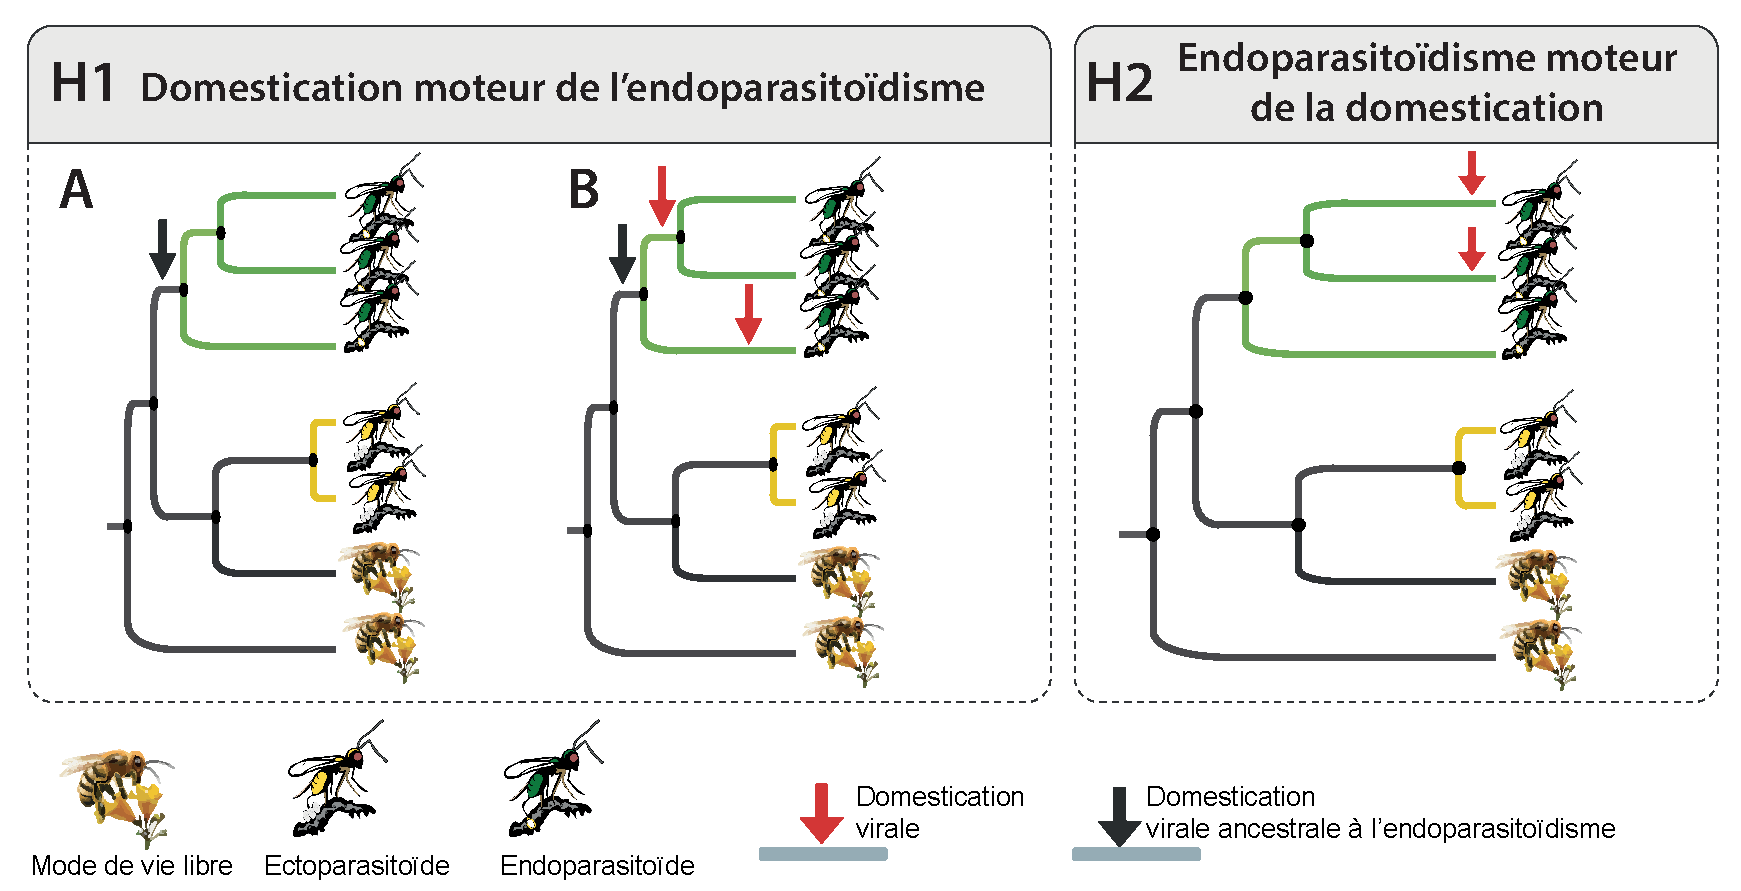
\includegraphics[width=\linewidth,height=\textheight,keepaspectratio]{PhD-master/figures/Endo_moteur_domestication.pdf}
\label{figure:Endo_moteur_domestication}
\end{figure}

Nous pourrions alors envisager ces deux hypothèses comme suit : \\

\textbf{Hypothèse 1}

Sous cette hypothèse, l'endogénisation et la domestication virale serait à l'origine de l'évolution de l'endoparasitoidisme. Cette hypothèse  peut être elle-même scindée en deux sous-hypothèses. La première (H1-A) impliquerait un évènement unique et ancestral de domestication ayant fortement favorisé l'apparition du mode de vie endoparasitoïde. La deuxième (H1-B) impliquerait également un évènement ancestral de domestication qui aurait été suivie de nombreux remplacements, à l'instar des syncitines chez les mammifères placentaire \citep{lavialle_paleovirology_2013}.\\ 

\textbf{Hypothèse 2}

Dans l'hypothèse alternative (H2), nous envisageons que l'évolution vers l'endoparasitoidisme n'implique pas de domestication virale, mais que plusieurs évènements de domestications, postérieurs à l'apparition du style de vie endoparasitoïde se seraient produits dans certaines lignées. Dans ce cas, ce serait le style de vie endoparasitoïde qui aurait favorisé la domestication de virus, via un avantage lié au contournement immunitaire. \\

Nous pourrions donc résumer H1 à une hypothèse selon laquelle la domestication aurait été un moteur de l'endoparasitoïdisme, alors que H2 serait l'hypothèse selon laquelle l'endoparasitoïdisme déjà bien établi, aurait été un moteur de la domestication.


\subsection{Évaluation de l'hypothèse H1}

Dans un premier temps, nous pouvons rechercher des arguments en faveur de la première hypothèse d'un seul évènement ancestral à l'endoparasitoïdisme (H1). Effectivement, dans nos données, nous observons plus d'évènements de domestication de virus dsDNA chez les endoparasitoïdes. Nous pourrions donc imaginer que toutes ces séquences proviennent d'un seul évènement ancestral. Seulement, ce n'est clairement pas le cas, car les gènes domestiqués ne présentent pas de signal phylogénétique dans ce sens, mais traduisent plutôt des évènements d'acquisitions indépendants. Ces données ne collent donc pas avec l'hypothèse (H1-A). En  revanche, l'hypothèse (H1-B) selon laquelle un évènement ancestral, suivi de plusieurs évènements de remplacements, serait envisageable.  Nous pourrions alors assister, comme chez les mammifères placentaires \citep{lavialle_paleovirology_2013}, à plusieurs événements récurrents de remplacements d'éléments viraux au cours de l'évolution, en gardant l'hypothèse d'une insertion ancestrale à l'origine de ce style de vie, mais qui en vue des remplacements, serait aujourd'hui impossible à détecter sur plus de 200 millions d'années d'évolution. De futures recherches pourraient supporter cette hypothèse en analysant, par exemple, les génomes d'autres espèces qui ont indépendamment évolué vers un mode de vie endoparasitoïde, comme les Diptères Tachinidae \citep{stireman_tachinidae_2006}. Sara Oukkal rédige d'ailleurs actuellement une partie de sa thèse sur ces points. 

Seulement, quelques espèces endoparasitoïdes de notre jeu de donnée ne présentaient pas d'évènement de domestication. En effet, dans le \hyperref[sec:chap1]{chapitre 1}, 3/37 des génomes endoparasitoïdes ne présentaient pas un seul EVE, et 15/37 endoparasitoïdes ne présentaient aucun évènement de domestication. Parmi ces parasitoïdes, certains ne presentaient dailleurs aucune trace de production de VLS. Par exemple, chez \textit{P. concolor} et \textit{P. lounsburyi}, aucun VLP ou PDVs n'a été détecté dans les glandes à venins et les ovaires des deux espèces \citep{mathe-hubert_comparative_2016}. Nous ne parvenons d'ailleurs pas à trouver de phénomène de domestication pour ces deux espèces. De plus, chez \textit{Eretmocerus}, les espèces étudiées ne présentent également pas de preuve de production de VLS \citep{gelman_host-parasite_2005}. Concernant \textit{Eretmocerus}, nous ne retrouvons d'ailleurs pas d'évènement de domestication de virus dsDNA. Nous pourrions ainsi imaginer, toujours sous l'hypothèse H1-B, qu'il y ait eu des pertes de ces fonctions virales chez ces espèces.


\subsection{Évaluation de l'hypothèse H2}

D'autres arguments font plutôt pencher la balance vers l'hypothèse (H2). 

\textbf{Pas de trace d'évènements aussi anciens que le clade des Parasitoida}\\
Le premier argument tient dans le fait que nous ne retrouvons aujourd'hui que des évènements postérieurs au groupe des Parasitoida. Par exemple, les plus anciens cas décrits à ce jour sont ceux des Microgastroïdes, il y a 100 millions d'années \citep{whitfield_virus_2003, bezier_bracovirus_2008, murphy_phylogeny_2008} et ceux découverts lors du \hyperref[sec:chap3]{chapitre 3} chez les Eucoilini, il y a 75 millions d'années. Cependant, ceci ne permet pas de rejeter complètement l'hypothèse H1-B impliquant des remplacements. \\

\textbf{Des stratégies n'impliquant pas de VLS endogénisés existent chez les endoparasitoïdes}\\
Chez de nombreuses espèces d'endoparasitoïdes, des stratégies d'inhibition du système immunitaire de l'hôte n'impliquant pas la production de VLS sont rencontrées. 
Par exemple, d'autres stratégies peuvent impliquer également des virus, mais non endogénisés. En effet, comme nous l'avons vu chez l'espèce \textit{Diachasmimorpha longicaudata}, il a pu être mis en évidence des effets protecteurs analogues aux polydnavirus et VLPs provenant d'un poxvirus mutualiste, sans pour autant présenter de domestication intra-génomique virus \citep{coffman_mutualistic_2020,coffman_viral_2022}, ou bien encore un ascovirus mutualiste (DpAV4) qui chez plusieurs espèces du genre \textit{Diadromus} permet lorsqu'il est injecté dans l'hôte, d'augmenter le succès du développement des progénitures \citep{stasiak_characteristics_2005}. Nous pourrions en revanche imaginer que ce sont ce genre d'interactions sur le long terme qui auraient participé à la rétention des gènes de ces virus mutualistes par ces guêpes au cours de l'évolution. \\

Enfin, chez certaines espèces endoparasitoïdes, le venin qui accompagne l'œuf est dépourvu de VLS \citep{moreau_venom_2015}. En effet, des espèces comme \textit{Pimpla hypochondriaca} et \textit{Pteromalus puparum} qui sont toutes des endoparasitoïdes de Lépidoptères, ou bien \textit{Aphidius ervi} qui est un endoparasitoïde de pucerons, présentent toutes des fonctions de contournement de l'immunité présent dans leur venin, sans pour autant produire de particules virales \citep{moreau_venom_2015}. Ceci constitue donc un contre-argument à l'hypothèse H1, car d'autres stratégies retrouvées chez des guêpes endoparasitoïdes existent sans présenter de trace de production de VLS. Néanmoins, nous pourrions envisager qu'il y ait eu, en particulier chez ces espèces, une perte secondaire de la production de VLS.\\ 

\textbf{Une "amélioration" de fonction apportée par la domestication chez les guêpes endoparasitoïdes?}\\
Nous pourrions formuler l'hypothèse que l'apport de la domestication virale aurait en quelque sorte "amélioré" le système pré-existant chez de nombreuses espèces endoparasitoïdes. Certains arguments vont en faveur de cette hypothèse. En effet, les venins d'endoparasitoïdes sont également impliqués dans des interactions synergiques avec les PDV/VLP dans certains systèmes hôte-endoparasitoïde \citep{asgari_venom_2006,asgari_venom_2011,schmidt_innate_2001}. Des études suggèrent que le venin renforce l'effet des PDVs. Par exemple chez \textit{Microplitis demolitor} sur les hémocytes de l'hôte (inhibition de l'étalement cellulaire) de manière dose-dépendante, et retarde également le développement de l'hôte \citep{strand_developmental_1991,strand_alterations_1991}. Le venin est également nécessaire pour l'entrée et le déballage des PDVs chez \textit{Cotesia melanoscela} \citep{stoltz_venom_1988}, et chez \textit{Cotesia rubecula}, les gènes de virulence ne sont même pas exprimés dans les hémocytes en l'absence de certains peptides présents dans le venin \citep{zhang_novel_2004} (voir \citep{moreau_venom_2015} pour revue). Par conséquent, étant donné que les systèmes VLS dépendent du venin injecté, il est probable que ces systèmes se sont adaptés à un système de production de venin existant qui ne comportait pas au préalable de VLS.\\

Enfin, certains des gènes ou protéines de virulence présents dans les polydnavirus et les VLPs sont dérivés des guêpes \citep{desjardins_comparative_2008,burke_systematic_2014, huguet_evolution_2012}, tandis que d'autres plus rares dérivent d'éléments transposables (TE) \citep{zhang_chromosome-level_2019, gauthier_chromosomal_2021}, et on imagine que ces gènes ont ensuite été transférés dans le provirus qui constituent \textit{in fine} les cercles d'ADN par exemple \citep{herniou_when_2013}. Ces gènes (ou leurs protéines codées) aujourd'hui présents dans les VLPs ou les PDVs étaient probablement déjà présents dans les génomes des guêpes avant la domestication et  rentraient déjà dans la composition du venin des guêpes ancestrales, participant ainsi à réguler le métabolisme et l'immunité de l'hôte. Les VLPs ou VLS auraient "simplement" constitué un moyen plus efficace pour délivrer ces facteurs de virulence aux cellules cibles. \\

\textbf{Conclusion sur cette partie}

Prises dans leur ensemble, ces observations tendent donc à favoriser la deuxième hypothèse (H2) selon laquelle l'endoparasitoïdisme ne serait pas né d'une domestication ancestrale, mais que plusieurs évènements de domestications seraient apparus indépendamment le long de la phylogénie des Hyménoptères, sans que tous les clades ne soient concernés. Et ceci se serait produit particulièrement au sein des clades endoparasitoïdes dont le style de vie aurait favorisé la rétention de ces gènes viraux à des fins d'adaptation face au système immunitaire de leurs hôtes.  


\section{La domestication comme moteur du succès évolutif}

Sur le plan évolutif, ces évènements de domestication ont probablement chamboulé la trajectoire évolutive des espèces concernées dont les descendants représentent aujourd'hui une grande diversité d'espèces. Le groupe des microgastroïde est un bon exemple. Il s'agit de l'ensemble des espèces dont l'ancêtre commun a vraisemblablement acquis puis domestiqués une batterie de gènes provenant d'un nudivirus ancestral il y a 100 millions d'années \citep{murphy_phylogeny_2008, whitfield_estimating_2002,banks_dissecting_2006}. Aujourd'hui, ce groupe représente une partie importante de la diversité des Ichneumonoidea avec 46,000 espèces estimées dans le monde \citep{rodriguez_extrapolations_2013}. 
Ces résultats suggèrent donc que sur de longues périodes, la domestication virale a contribué activement à la radiation du clade.\\
De la même manière, nous avons observé dans le \hyperref[sec:chap3]{chapitre 3} qu'une domestication virale ancienne chez l'ancêtre commun du clade diversifié des Eucoilini pourrait avoir eu des conséquences très importantes dans l'évolution de ce clade via la production de VLPs que nous observons chez au moins 2 genres de ce groupe. \\

\section{Domestication de virus filamenteux chez les Eucoilini}

En ce qui concerne les Eucoilini, nous avons pu identifier deux cas distincts d'endogénisation. Le premier cas concerne un pool de 18 gènes domestiqués chez presque toutes les espèces d'Eucoilini étudiées, dont l'ancêtre commun aurait acquis ces gènes il y a environ 75 millions d'années \citep{blaimer_comprehensive_2020}. Le second cas, plus récent, concerne un pool de 9 gènes provenant d'un seul membre de ce groupe dans le genre \textit{Rhoptromeris}. Dans les deux cas, les génomes viraux endogénisés provenaient de virus filamenteux, LhFV étant le plus étroitement lié au premier événement et LbFV au second (\figurename{\ref{figure:Microscopie_trybliographa}}).

\begin{figure}[!htpbt]
\captionsetup{font=footnotesize}
 \centering
  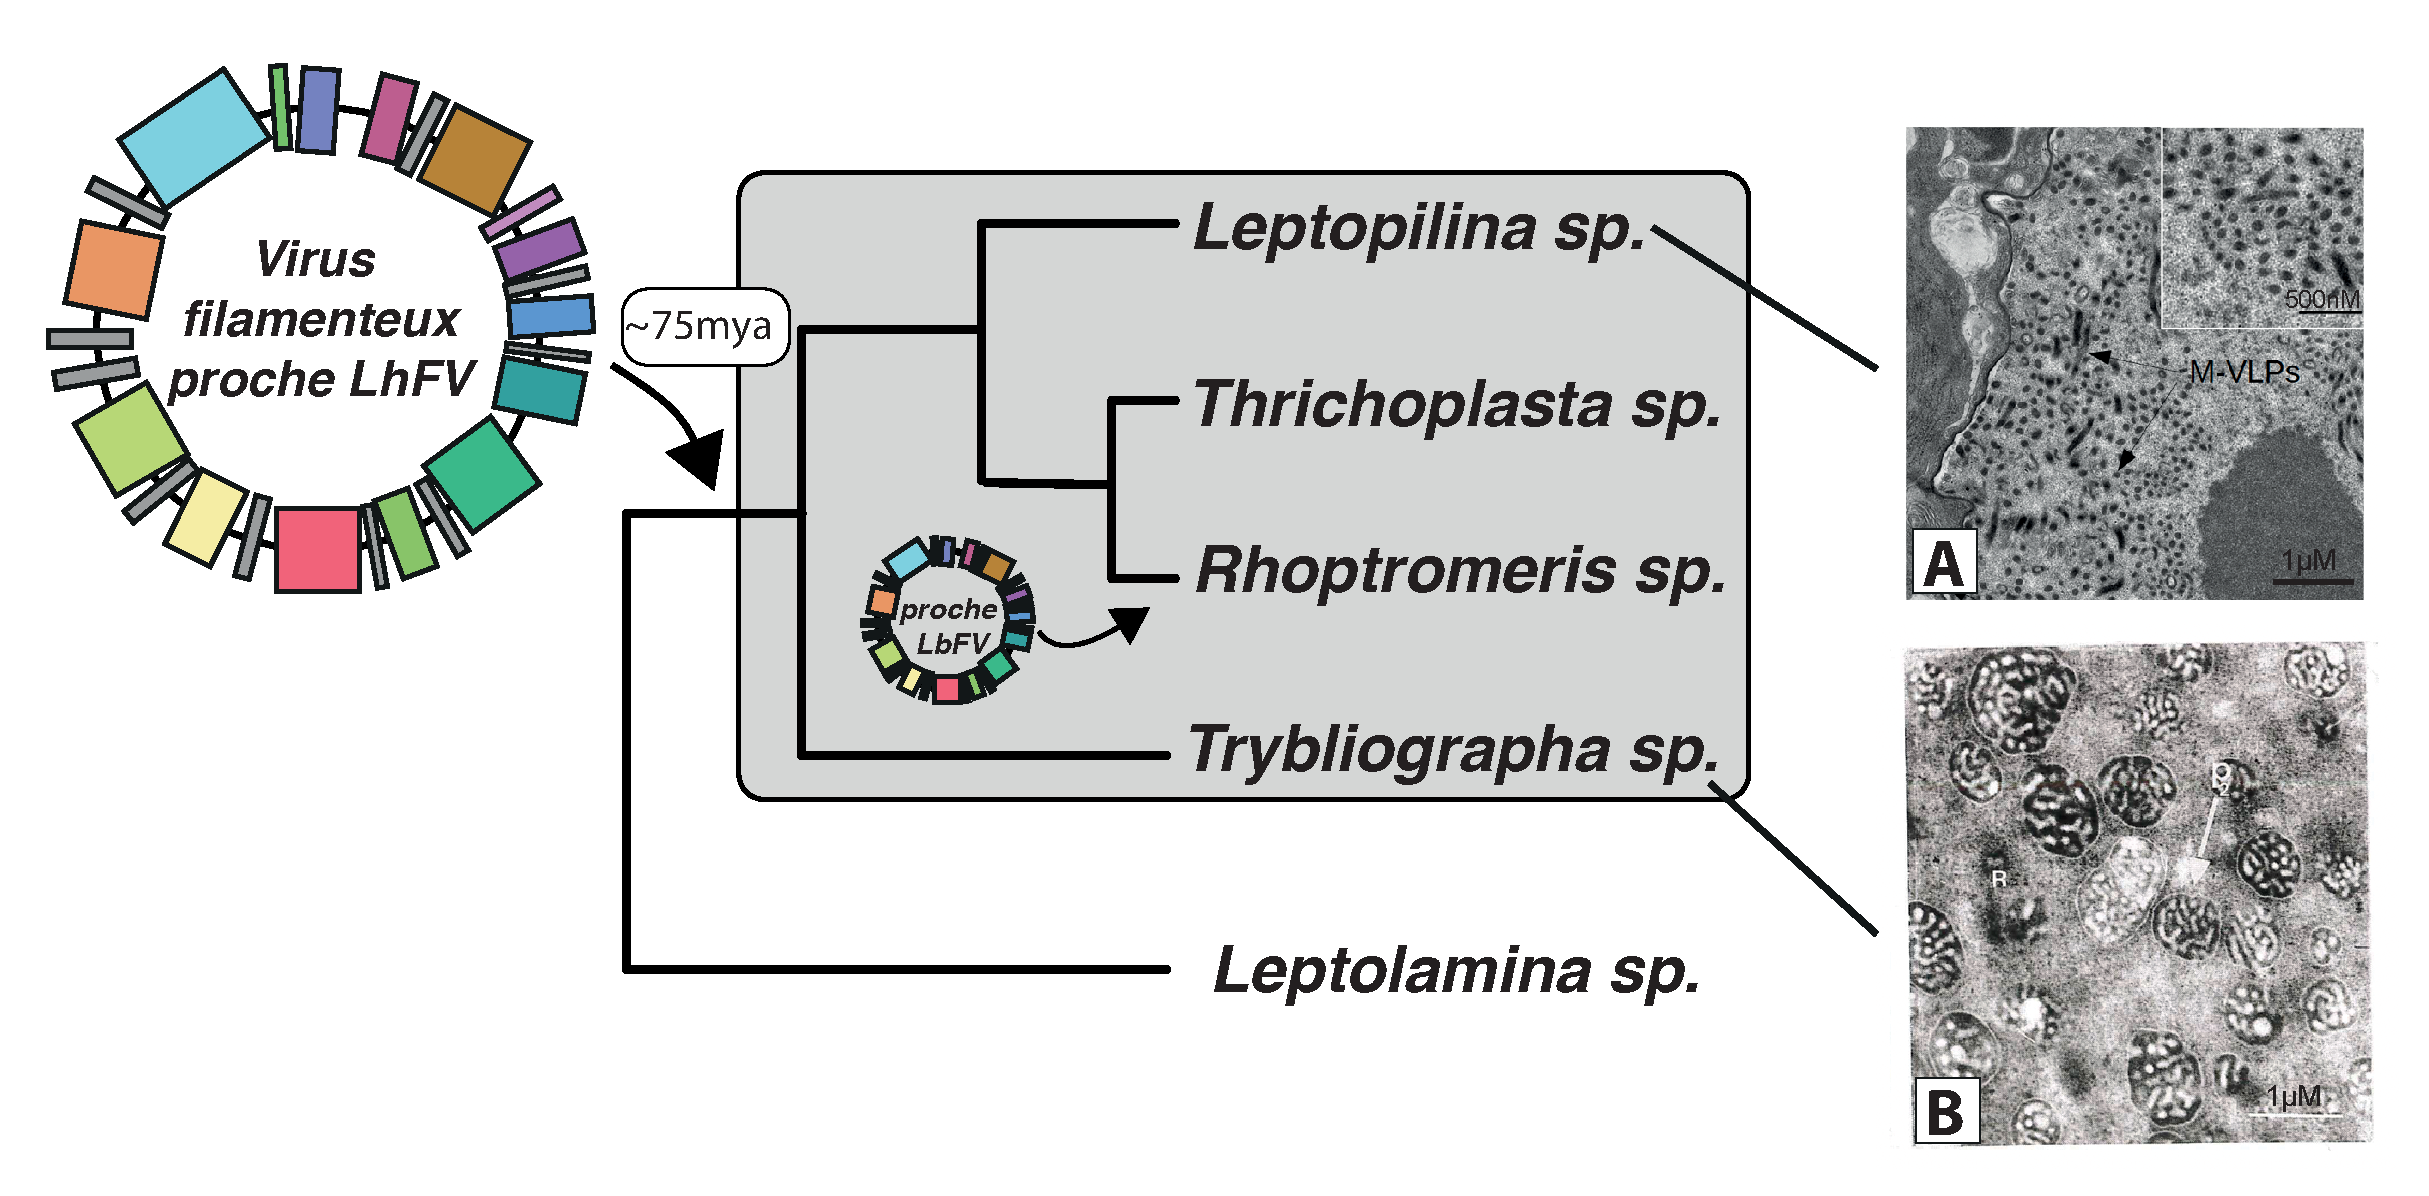
\includegraphics[width=\linewidth,height=\textheight,keepaspectratio]{PhD-master/figures/Microscopie_trybliographa.pdf}
\caption[Discuss:Résumé graphique des deux évènements indépendants d'endogénisations chez les Eucoilini]{\textbf{Résumé graphique des deux évènements indépendants d'endogénisations chez les Eucoilini}. VLPs produits dans la glande à venin de \textit{Lepoptilina boulardi} (A) et \textit{Trybliographa rapae} (B)  photos de (Di Giovanni et al., 2020) et D.Poinçot et K.Haddj E PhD 1999.}
\label{figure:Microscopie_trybliographa}
\end{figure}

Il est clair que les 18 EVEs de l'événement initial jouent un rôle dans le développement des VLPs. 13 de ces 18 EVEs sont spécifiquement exprimées dans la glande à venin au début du stade nymphal de la guêpe, lorsque les VLPs sont synthétisées, comme décrit dans \cite{di_giovanni_behavior-manipulating_2020}. Par conséquent, nous nous attendons à ce que les cinq EVEs supplémentaires retrouvés dans notre analyse au \hyperref[sec:chap3]{chapitre 3} présantent les mêmes profils d'expression. Par ailleurs, comme on pourrait s'y attendre pour des gènes impliqués dans la production de VLPs, nous observons des signaux extrêmement forts de sélection purificatrice pour tous les EVEs provenant de l'événement d'endogénisation initial, y compris pour les 5 nouveaux (\figurename{\ref{figure:Cynipids_VLPS_updated_discuss}}-1).\\ 

Concernant les fonctions de ces EVEs, nous retrouvons les gènes \textit{lef-4}, \textit{lef-9} et \textit{lef-8} chez toutes les espèces concernées par l'évènement ancestral chez les Eucoilini. Avec le facteur d'initiation (\textit{lef-5}) identifié par mon analyse, ceci suggère que toutes ces guêpes possèdent les gènes nécessaires pour former un complexe complet d'ARN polymérase (\figurename{\ref{figure:Cynipids_VLPS_updated_discuss}}-3). De plus, la présence d'une \textit{helicase} et \textit{ADN polymerase} filamenteuses suggère qu'une partie de la machinerie ancestrale de réplication de l'ADN viral est encore fonctionnelle chez les espèces Eucoilini (\figurename{\ref{figure:Cynipids_VLPS_updated_discuss}}-2). En effet, il a été démontré que dans ce système, 10 des 13 EVEs sont amplifiés chez ces guêpes (Di Giovanni et al., 2020). L'hypothèse la plus vraisemblable étant que c'est l'ADN polymérase du virus filamenteux (ORF58) qui permet cette amplification qui augmenterait donc leur profil d'expression des EVEs (Di Giovanni et al., 2020). Plusieurs gènes sont également probablement impliqués dans l'enveloppement des protéines de virulence (\textit{ac81}), le développement des membranes lipidiques (\textit{lcat}), et éventuellement l'entrée des composants viraux dans les cellules hôtes par liaison à des récepteurs de surface cellulaire (\textit{LhFV contig223 orf23}) (\figurename{\ref{figure:Cynipids_VLPS_updated_discuss}}-4). Ce dernier gène (LhFV contig223 orf23) est présent chez tous les Eucoilini, mais chez \textit{Rhoptromeris}, il est probablement le résultat d'un remplacement suite au deuxième événement d'endogénisation. Par conséquent, il est possible que l'apparition d'une deuxième copie homologue de cette protéine à ce moment ait été fortement sélectionnée, car elle aurait conféré un avantage (\figurename{\ref{figure:Cynipids_VLPS_updated_discuss}}-4).\\

\begin{figure}[!htpbt]
\captionsetup{font=footnotesize}
 \centering
  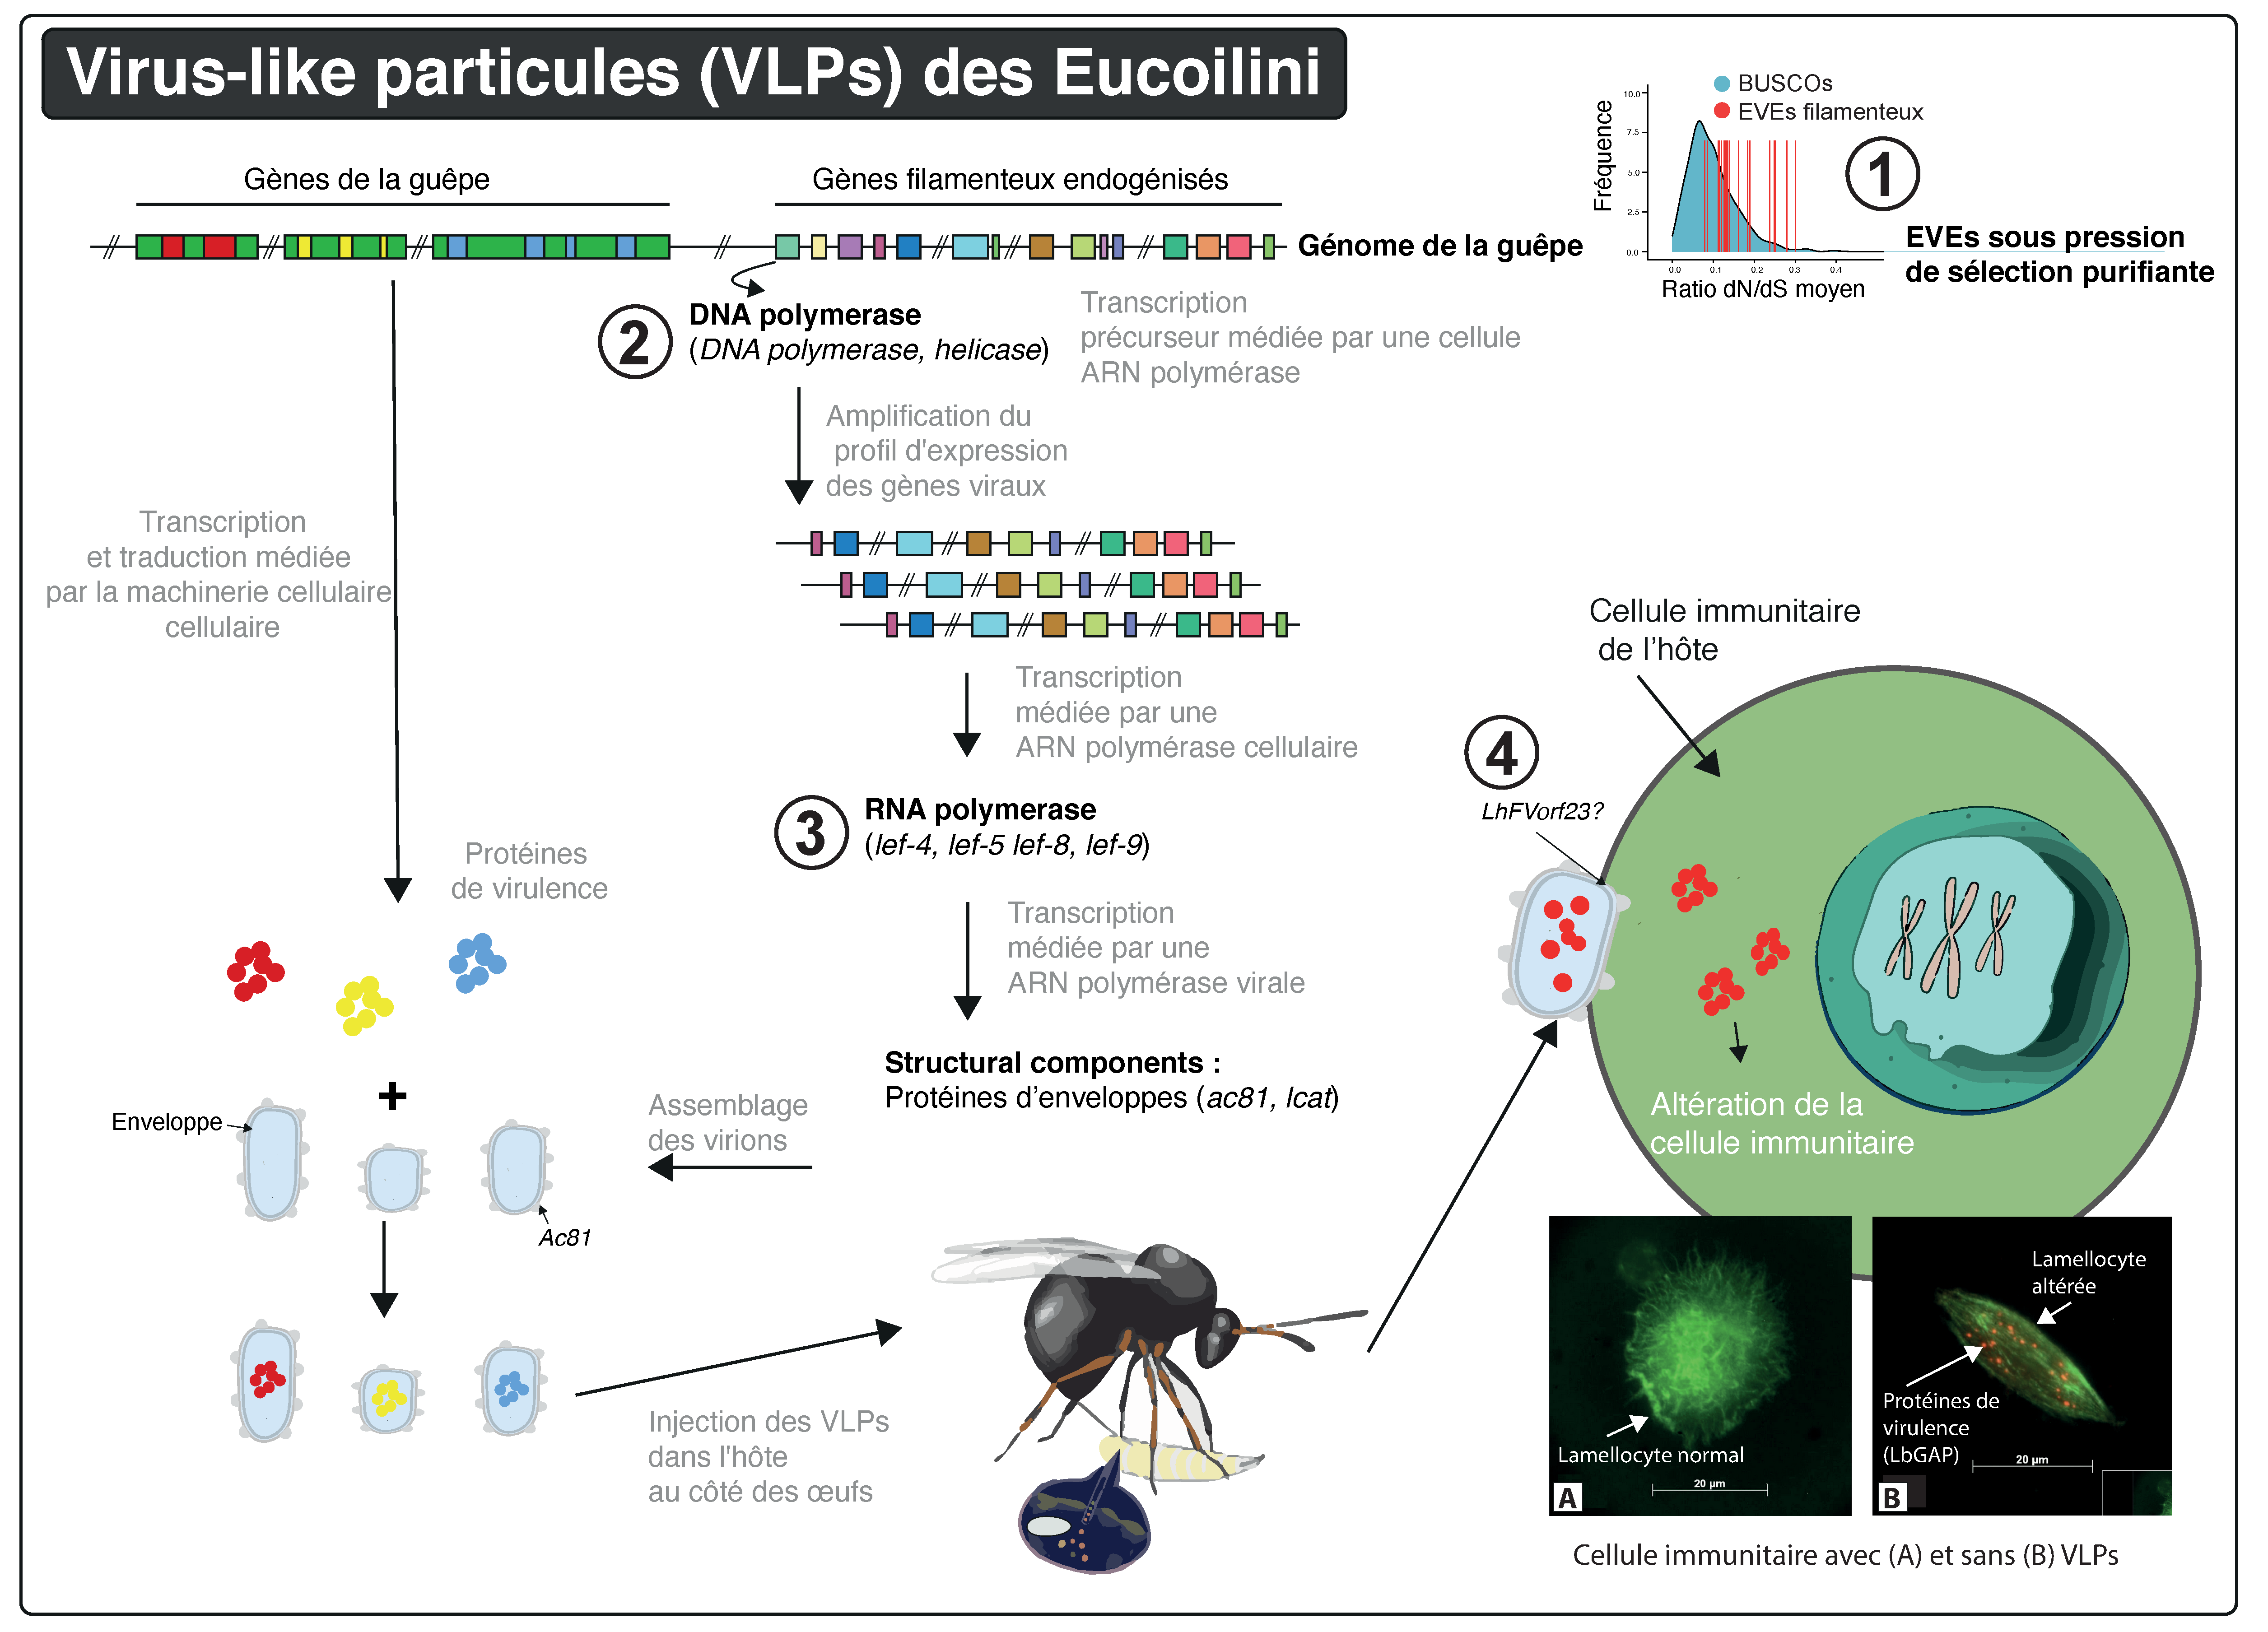
\includegraphics[width=\linewidth,height=\textheight,keepaspectratio]{PhD-master/figures/Cynipids_VLPS_updated_discuss.pdf}
\caption[Discuss:Résumé graphique putatif de la machinerie virale filamenteuse produisant des VLPs chez les Eucoilini]{\textbf{Résumé graphique putatif de la machinerie virale filamenteuse produisant des VLPs chez les Eucoilini}.}
\label{figure:Cynipids_VLPS_updated_discuss}
\end{figure}

Finalement, sur la base de l'ensemble de ces données, nous disposons de suffisamment d'éléments pour conclure que chez ces Eucoilini, les EVEs d'origine filamenteux sont très probablement impliqués dans la formation des VLPs. Dans le cas contraire où seuls certaines espèces de ce groupe auraient usage de ces VLPs, nous nous attendrions à ce que les 18 EVEs chez ces espèces ait dégénéré, or, tous ces gènes sont intacts après plus de 75 millions d'années d'évolution. De plus, la présence de VLPs dans les glandes à venin de l'espèce \textit{Trybliographa rapae} la plus basale du groupe Eucoilini concernée par l'événement, renforce cette hypothèse (thèse de Nabila Kacem Haddj El Mrabet en 1999) (\figurename{\ref{figure:Microscopie_trybliographa}}).\\ 

À la lumière de ces résultats, nous pourrions supposer que, tout comme les Microgastroïdes et leurs polydnavirus, la production de VLPs par les Eucoilini aurait également contribué au succès écologique et à la radiation du groupe. En effet, parmi les Figitidae, qui comportent près de 140 genres pour 1,569 espèces de guêpes, la sous-famille des Eucoilinae est de loin la plus riche en espèces avec plus de 80 genres et plus de 900 espèces décrites, soit près de 33\% de la diversité des Figitidae \citep{ronquist_phylogeny_1995}. Connaitre la diversité spécifique que représente les Eucoilini dans tout ça en revanche est plus difficile. Mais par exemple, le complexe "\textit{Eucoila}/\textit{Trybliographa}" au sein de cette tribu est l'un des groupes d'eucoilines les plus communs et les plus riches en espèces dans l'hémisphère nord (thèse de Mattias Forshage). \\

Par ailleurs, d'autres éléments pourraient nous faire penser que cet évènement de domestication a participé au succès évolutif de ce groupe. En effet, les résultats du \hyperref[sec:chap2]{chapitre 2} permettent d'estimer l'âge de l'évènement d'endogénisation virale entre 55 et 100 millions d'années, ce qui correspond à peu près à la période durant laquelle les hôtes Diptères (Schizophora) des Eucoilini ont commencé à se diversifier (entre 55 et 60 millions d'années) \citep{wiegmann_episodic_2011}. Ainsi, nous pourrions avancer que cette innovation génétique soudaine aurait permis à ces guêpes de coloniser et de s'adapter à leurs hôtes Schizophora au cours de la radiation du groupe.\\

Pour que ces deux événements d'endogénisation aient pu se produire indépendamment dans la lignée des Eucoilini (\hyperref[sec:chap3]{chapitre 3}) et plus généralement chez de nombreuses autres espèces endoparasitoïdes (\hyperref[sec:chap2]{chapitre 2}), il doit y avoir eu une longue période d'interaction étroite entre les Filamentoviridae et les guêpes. Dans la partie suivante, je discuterai les particularités de cette relation. 

\section{Les Filamentoviridae}

\subsection{Filamentoviridae : Préférence pour les endoparasitoïdes?}

Tous les Filamentoviridae analysés dans le \hyperref[sec:chap2]{chapitre 2} ont été découverts chez des guêpes endoparasitoïdes (\figurename{\ref{figure:Heatmap_NCBI4}}-A), cependant, pour éviter les biais inhérents aux thèmes de recherche de nos deux équipes, qui se sont surtout concentrées sur les endoparasitoïdes, nous avons recherché de manière systématique la présence d'éléments génétiques filamenteux dans des bases de données publiques (NBCI et BIPPA). Et ceci, en incluant tous les génomes d'Hyménoptères, mais également des hôtes putatifs des guêpes que sont les Lépidoptères et les Diptères. Ainsi, l'analyse systématique de 2815 génomes (couvrant 1576 espèces) n'a trouvé aucune preuve de la présence de génome de Filamentoviridae sauf chez des espèces endoparasitoïdes (9 au total si nous incluons tous les filamenteux connus). (\figurename{\ref{figure:Heatmap_NCBI4}}-B). \\

\textbf{Distribution intra-Hyménoptères}

Plus spécifiquement, au sein des Hyménoptères, les virus filamenteux semblent se répliquer préférentiellement chez les espèces endoparasitoïdes, puisque 40 des 87 génomes endoparasitoïdes analysés contenaient des EVEs contre seulement 3 des 209 Hyménoptères vivant librement et 0 des 29 ectoparasitoïdes. Aussi, il semblerait qu'à l'échelle des Hyménoptères, les virus filamenteux se soient spécifiquement adaptés aux Hyménoptères présentant un mode de vie endoparasitoïde, dont elles tirent, peut-être, profit. En effet, ce mode de vie pourrait représenter une niche écologique favorisant le maintien et la propagation de ces virus au sein des populations de guêpes, à la fois verticalement de la mère à la progéniture \citep{martinez_additional_2016, coffman_viral_2022} et horizontalement entre parasitoïdes non apparentés partageant le même hôte \citep{varaldi_infectious_2003,stasiak_characteristics_2005}.\\

Nos analyses de datation de la famille en \hyperref[sec:chap3]{chapitre 3} apportent également des éléments pour alimenter ces réflexions. Ces analyses ont révélé que les Filamentoviridae auraient divergé il y a entre 233 à 370 millions d'années (\figurename{\ref{figure:Cynipoidea_dsDNA_datation_plot}}), ce qui coïncide avec la période où les Hyménoptères ont commencé à se diversifier entre le Carbonifère et le Trias (239-329 millions d'années) \citep{peters_evolutionary_2017}. Ces données donnent à penser que l'origine de ces virus est sensiblement plus ancienne que celle du principal clade de guêpes parasitoïdes (les "parasitoida") qui ont divergé entre 195 et 266 millions d'années. Nous pourrions donc imaginer que les ancêtres filamenteux se seraient d'abord développés en infectant les premiers Hyménoptères avant de se spécialiser sur des Hyménoptères au style de vie endoparasitoïdes.\\

\textbf{Distribution chez les hôtes des parasitoïdes}

Nous retrouvons également la présence de gènes filamenteux dans les génomes de Diptères et de Lépidoptères, mais en bien plus faible fréquence que chez les Hyménoptères (\figurename{\ref{figure:Heatmap_NCBI4}}-A et B). Ces deux ordres non Hyménoptère sont des hôtes privilégiés pour de nombreux Hyménoptères parasitoides. Ces insertions peuvent provenir d'infections filamenteuses passées ou en cours. De manière intéressante, une étude antérieure a mis en évidence des virus filamenteux se reproduisant chez les lépidoptères \citep{styer_new_1987}. Cependant, puisqu'aucune donnée de séquence n'est disponible pour ces virus, nous ne pouvons pas affirmer qu'ils appartiennent à la famille des Filamentoviridae. Dans nos données, nous ne retrouvons aucun signe d'infection en cours. En effet, en cas d'infection, on s'attendait à retrouver la plupart des gènes cœurs dans les scaffolds séquencés. Au contraire, nous n'avons retrouvé que quelques gènes, qui, de plus, se retrouvent pour la plupart dans des scaffolds trop grands pour correspondre à un génome viral. 

Bien que les données n'apportent pas de preuve de l'existence de lignées de Filamentoviridae infectant les Lépidoptères ou les Diptères, nous ne pouvons pas exclure qu'une partie inconnue de la diversité des Filamentorividae se soit spécialisée chez les Lépidoptères, voire les Diptères.\\

\textbf{Perspective de travail sur cette partie}

En perspective de ces travaux, afin d'expliquer davantage cette préférence pour les endoparasitoïdes, nous pourrions envisager d'étendre notre recherche systématique de virus filamenteux à l'échelle des données brutes SRA. En effet, nous pourrions imaginer que les auteur.ices.s des génomes assemblés aient arbitrairement supprimé tout scaffold dérivé d'un virus, nous empêchant ainsi de constater la présence de scaffolds filamenteux libres chez les espèces non endoparasitoïdes. Cependant, il n'y a aucune raison de croire que ce processus ne soit envisagé que pour les génomes des Lépidoptères et des Diptères et non pour les Hyménoptères endoparasitoïdes. De plus, ces analyses mériteraient d'être poursuivies en recherchant sur une plus large gamme d'organismes la présence de virus filamenteux exogènes ou endogènes afin de vérifier si seuls ces insectes sont concernés. Dans le cas d'une préférence pour le mode de vie endoparasitoïde, il n'y a aucune raison de penser que des traces de virus filamenteux seraient présents chez des espèces qui n'interagissent pas avec ce mode de vie. Enfin, nous avons l'intention d'étudier plus précisément l'effet du mode de vie endoparasitoïde sur l'existence de ces virus en intégrant l'inertie phylogénétique, qui n'est pas encore prise en compte dans nos recherches, car elle nécessite d'obtenir une phylogénie complète des espèces analysées. \newpage


\subsection{Filamentoviridae : Une source d'innovation génétique ?}

\begin{figure}[H]
\captionsetup{font=footnotesize}
 \centering
  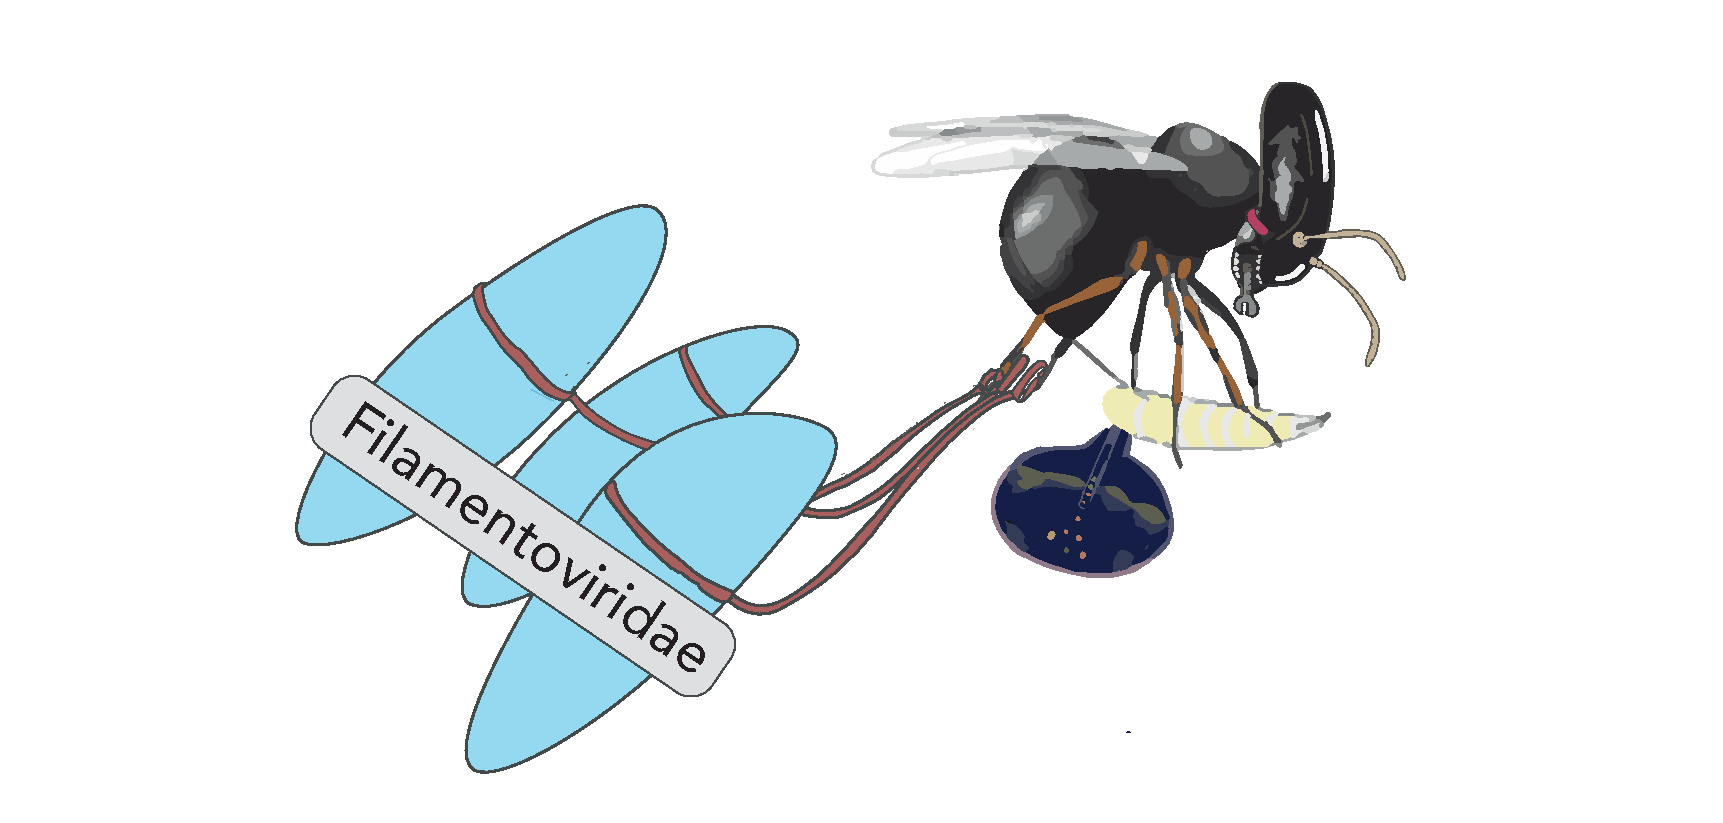
\includegraphics[width=\linewidth,height=\textheight,keepaspectratio]{PhD-master/figures/Domestication_illustration_Eucoilini.pdf}
\label{figure:Domestication_illustration_Eucoilini}
\end{figure}

\textbf{Du côté des guêpes}

Au moins deux fois par le passé, il y a 75 millions d'années chez les Eucoilini et plus récemment chez une espèce de Platygastroidea (\textit{P.orseoliae}), nous avons montré que l'insertion de virus filamenteux a pu entraîner une domestication moléculaire. Dans le premier scénario présenté, la fonction est orientée vers la synthèse de VLPs impliqués dans la protection de la progéniture contre le système immunitaire de l'hôte. Dans le second scénario, plus récent, cela est moins évident et il faudrait des preuves supplémentaires, comme la transcriptomique et la microscopie électronique, pour tester nos hypothèses selon lesquels les ORFs filamenteux sont à l'origine de la production de VLPs. D'autres cas d'endogénisation ont également été proposés sans révéler de preuve de domestication comme chez \textit{Dolichomitus} \citep{burke_endogenization_2020}, ou bien plusieurs espèces d'Hyménoptères, Diptères et Lépidoptères dans les \hyperref[sec:chap1]{chapitre 1} et \hyperref[sec:chap2]{chapitre 2}.\\

Aussi, il apparait que les phénomènes de domestication tels qu'envisagés lors de la production de structures virales sont encore rares du côté des virus filamenteux. Néanmoins, nous montrons tout de même dans les \hyperref[sec:chap1]{chapitre 1} et \hyperref[sec:chap2]{chapitre 2} plusieurs cas d'insertions filamenteux potentiellement adaptatives et l'étude de ces insertions serait nécessaire pour connaitre leurs fonctions spécifiques. Ainsi, si ces relations filamenteux-endoparasitoïdes existent, nous devrions, en continuant à séquencer les endoparasitoïdes, trouver de plus en plus d'exemples de domestication de ce type. \\

\newpage

\textbf{Du côté des hôtes des guêpes}

Nous venons d'aborder l'aspect endoparasitoïde, mais nous pouvons également discuter de la nature adaptative des insertions filamenteuses chez les hôtes des guêpes parasitoïdes.

Parmi les Diptères et les Lépidoptères, deux ordres attaqués par les guêpes endoparasitoïdes, nous avons constaté dans le \hyperref[sec:chap2]{chapitre 2} que la majeure partie de ces EVEs filamenteux étaient dégradés, ce qui suggère qu'il s'agit d'insertions plutôt anciennes et non fonctionnelles (\figurename{\ref{figure:Heatmap_NCBI4}}-B). Quelques-uns de ces gènes sont en revanche toujours intacts et pourraient toujours êtres fonctionnels dans le génome de certains Diptères ou Lépidoptères. Ces gènes encore intacts pourraient provenir d'insertions trop récentes pour voir l'apparition de codons stop prématurés suite à une pseudogénisation. Néanmoins, dans la littérature, des études ont déjà montré que les guêpes parasitoïdes et leurs hôtes subissent des transferts de gènes médiés par des virus endogènes \citep{muller_investigating_2022, gasmi_recurrent_2015,di_lelio_evolution_2019}. Par exemple, un THG d'un gène de guêpe, "\textit{Sl gasmin}", surement médié par un polydnavirus (PDVs), joue un rôle central dans la médiation de la phagocytose bactérienne dans les hémocytes de papillon de nuit \textit{Spodoptera littoralis} \citep{di_lelio_evolution_2019}. Nous pourrions donc imaginer que chez les espèces présentant des PDVs et des virus filamenteux, des transferts de gènes aient été médiés de la même façon des génomes filamenteux vers les génomes des Lépidoptères. D'autres exemples montrent également des THG d'une famille de protéines toxiques virales appelées parasitoid killing factor (PKF). Dans ce cas, ces facteurs sont retrouvés dans les génomes des virus présent chez les Lépidoptères (entomopoxvirus, ascovirus, et baculovirus). Certaines espèces de lépidoptères auraient acquis des PKF provenant de ces virus, et ceux-ci fournissent des armes spécifiques qui permettent de contrer les attaques de certains parasitoïdes en particulier \citep{gasmi_horizontally_2021}.\\ 

Ces deux exemples laissent entrevoir des routes de transmission potentielles entre les virus filamenteux et les Lépidoptères, soit via l'interaction hôte-parasitoïde (médié possiblement par des PDVs), soit via l'interaction directe entre Filamenteux-Lépidoptères.

De manière intéressante, certains EVEs filamenteux sont présents chez plusieurs espèces de Lépidoptères du même genre, ce qui suggère que leur endogénisation pourrait avoir eu lieu chez leur ancêtre commun. En effet, par exemple chez 4 espèces du genre \textit{Apodemia} présentant des homologies de séquence avec LbFVorf20, on retrouve effectivement une phylogénie du gène qui place ces séquences dans un groupe monophylétique. De même par exemple dans le cas du gène \textit{pif-5} retrouvé chez 3 espèces du genre \textit{Junonia}. Cependant, à regarder les phylogénies des gènes, on se rend compte que ces séquences forment un râteau, ce qui est peu probable sous l'hypothèse d'une endogénisation chez l'ancêtre commun de ces deux genres, car nous devrions observer des différences le long des séquences (\figurename{\ref{figure:Host_filamentous_EVES_phylogeny}}).\\

Une hypothèse que nous pourrions formuler concernant l'acquisition de ces gènes pourrait être celle d'un transfert médié par des baculovirus de Lépidoptères. Ce genre de cas a déjà été décrit dans la littérature. En effet, \cite{gilbert_continuous_2016} ont par exemple pu montrer, en analysant les génomes de plusieurs populations de baculovirus infectieux de Lépidoptères, des transferts d'éléments transposables et d'autres séquences provenant des Lépidoptères vers les génomes des baculovirus (4.8\% des génomes viraux séquencés portaient au moins une insertion). Cette étude a ensuite fournit également des arguments suggérant l'implication des baculovirus en tant que vecteurs de transfert horizontal entre lépidoptères (voir aussi \citep{keeling_functional_2009,jehle_horizontal_1998,gilbert_population_2014}). En ce qui concerne les 2 gènes évoqués précédemment, nous pourrions imaginer que les Lépidoptères puissent être infectés par une lignée de virus filamenteux qui interagirait avec les baculovirus dans les cellules de ces insectes. Lors de ces interactions, des échanges génétiques auraient pu avoir lieu entre les filamenteux et les baculovirus. Certains ET Lépidoptères présents dans les génomes de baculovirus auraient ainsi pu médier un transfert de ces gènes filamenteux dans un second temps entre espèces  de Lépidoptères. Ce qui pourrait expliquer ce fameux râteau dans la phylogénie. Nous pourrions également imaginer que les génomes de virus filamenteux agissent même sans l'intermédiaire des baculovirus, et soient également des vecteurs de transfert horizontaux. Bien évidemment, pour confirmer ou non ces hypothèses, de nombreuses analyses seraient nécessaires, comme vérifier la présence d'évènements de transpositions dans les séquences flanquants ces gènes, ou bien vérifier que le long des génomes de baculovirus, nous trouvions effectivement des gènes filamenteux. 

\begin{figure}[!htpbt]
\captionsetup{font=footnotesize}
 \centering
  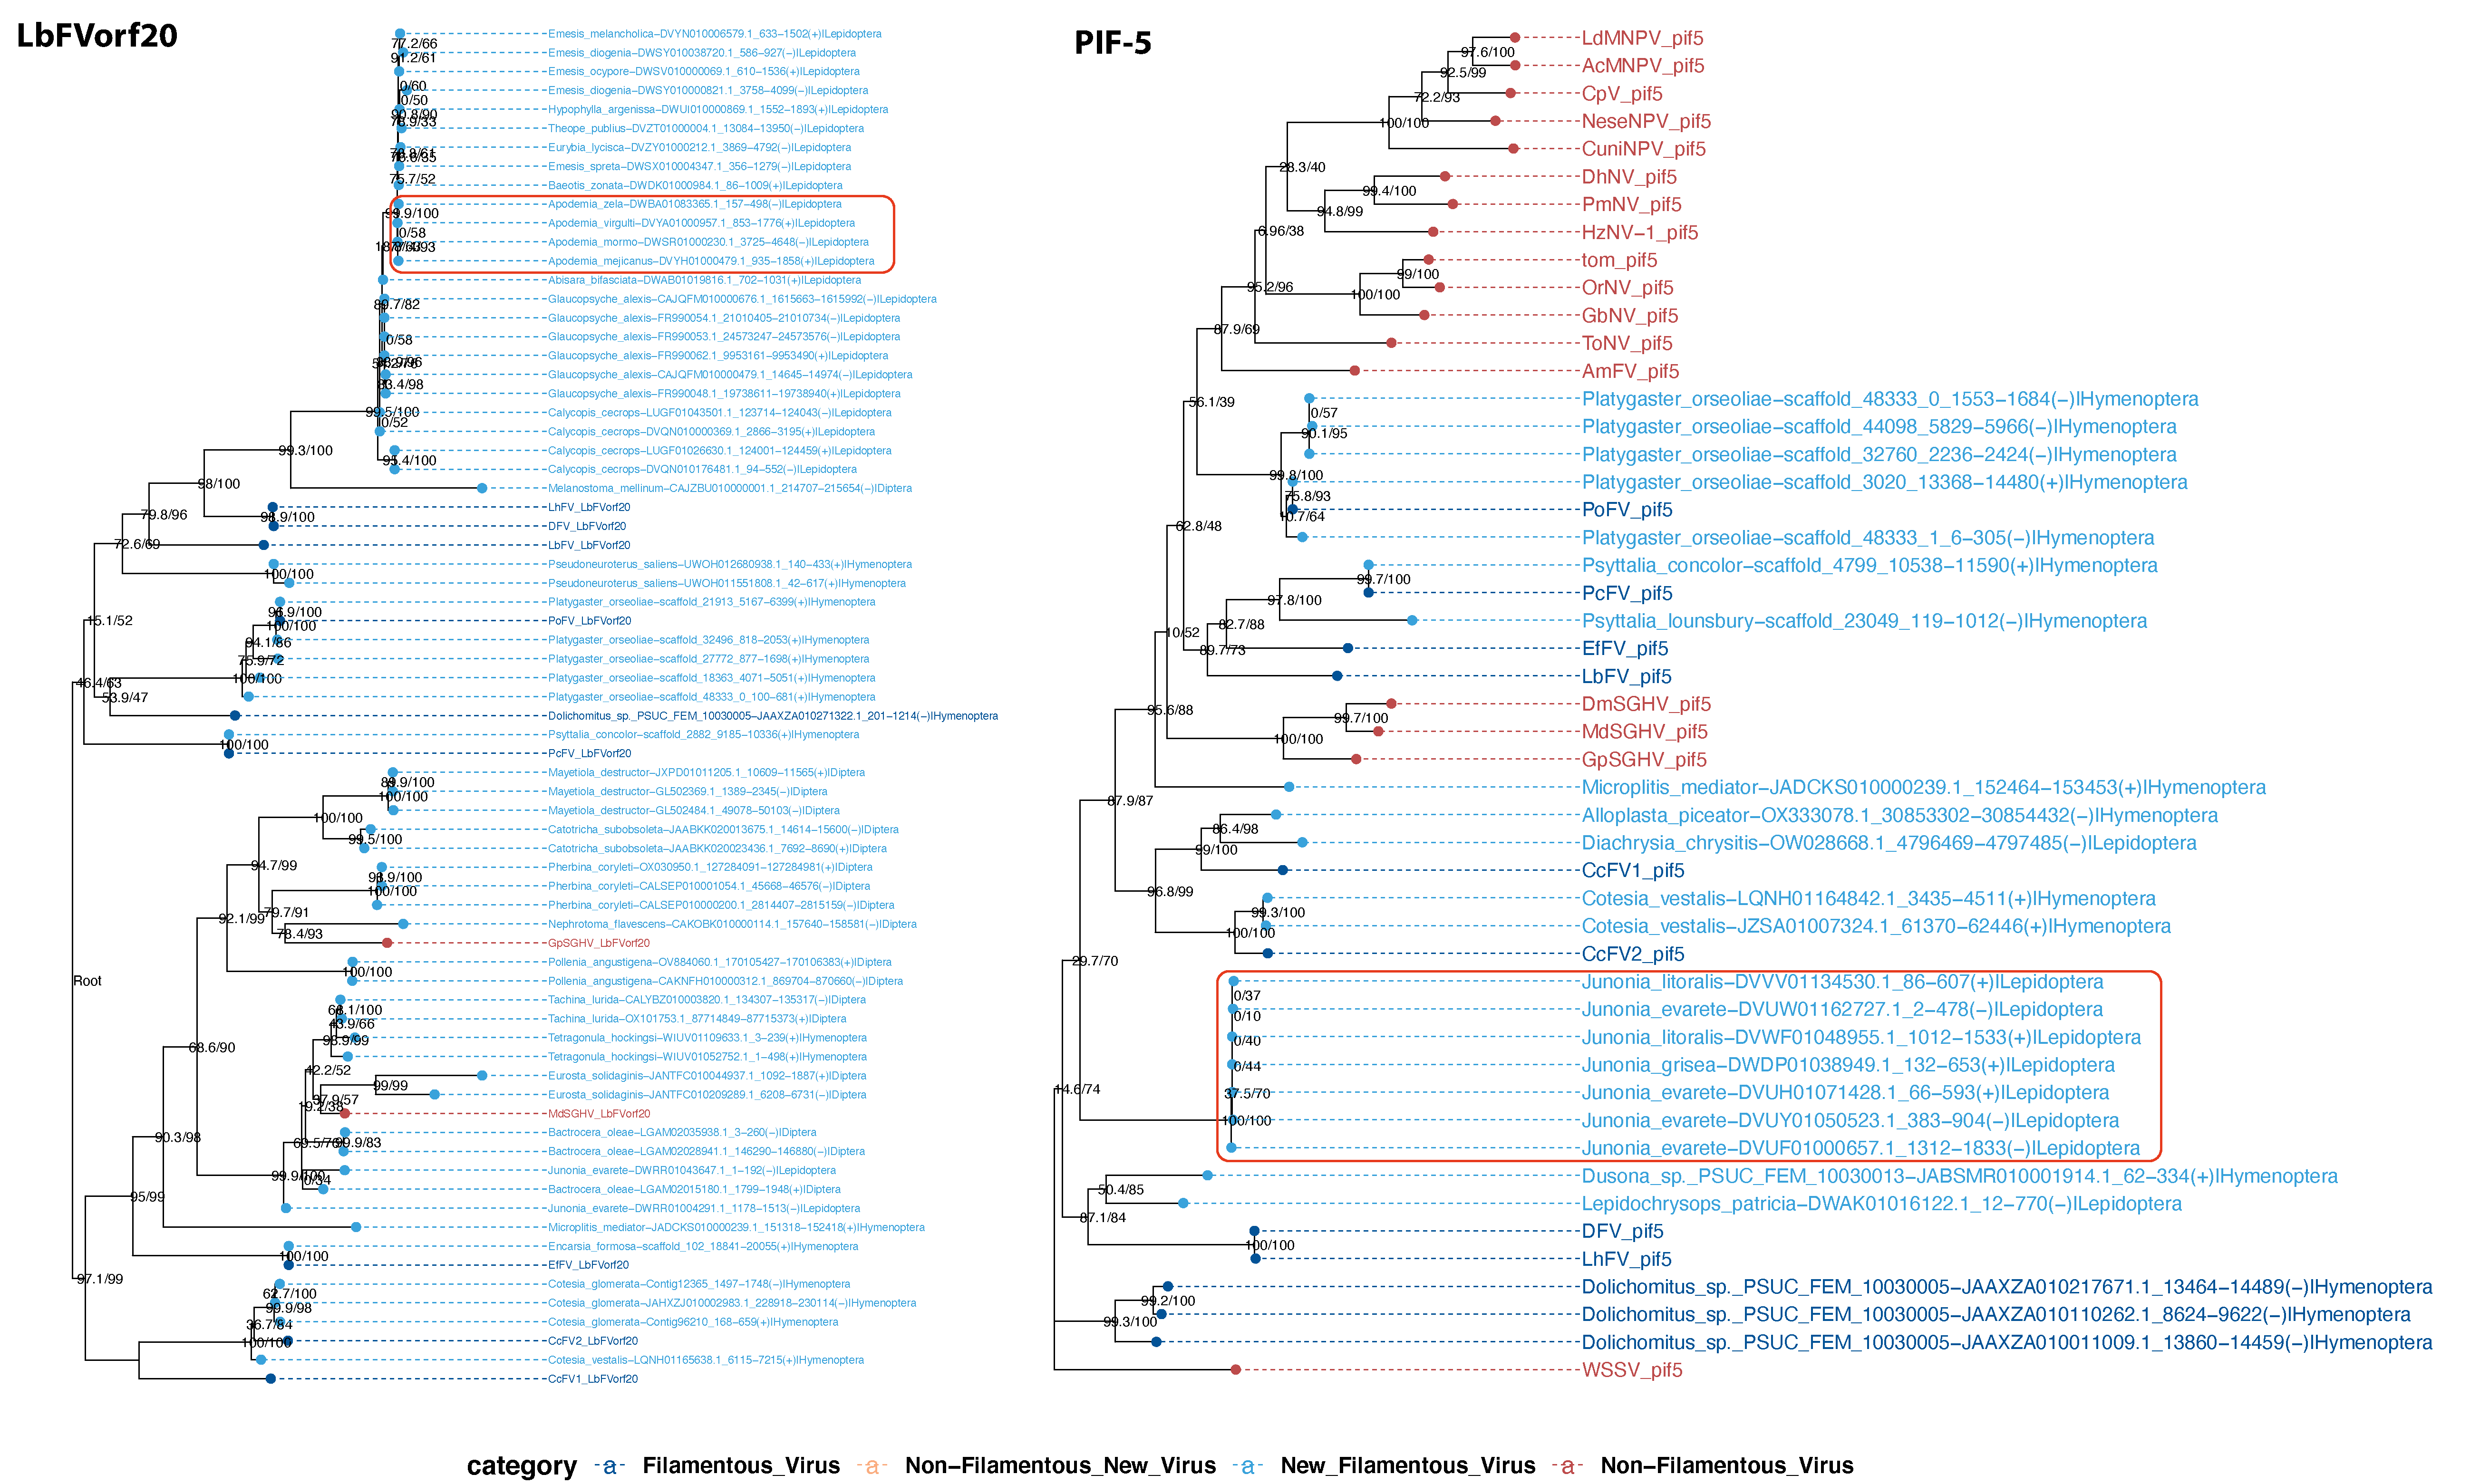
\includegraphics[width=\linewidth,height=\textheight,keepaspectratio]{PhD-master/figures/Host_filamentous_EVES_phylogeny.pdf}
\caption[Discuss:Phylogénies des gènes filamenteux LbFVorf20 et pif-5]{\textbf{Phylogénies des gènes filamenteux LbFVorf20 et pif-5}. Ces phylogénies comportent des séquences de virus filamenteux (bleu foncé), d'autres virus (rouge), et d'EVEs chez des espèces d'insectes dont l'ordre est indiqué après le pipe sur chaque séquence (bleu clair). Les figures d'alignements protéiques de ces deux gènes, comprenant uniquement les espèces du genre \textit{Glaucopsyche} et \textit{Apodemia} avec toutes les séquences virales, sont disponibles via les liens GitHub suivants : \href{https://github.com/BenjaminGuinet/PhD_defense/blob/main/Discussion/LbFVorf20_lepido_filamentous_MSA.pdf}{LbFVorf20} et \href{https://github.com/BenjaminGuinet/PhD_defense/blob/main/Discussion/Pif5_lepido_filamentous_MSA.pdf}{Pif5}.}
\label{figure:Host_filamentous_EVES_phylogeny}
\end{figure}


\newpage

\subsection{Filamentoviridae : Manipulation du comportement de ponte, une caractéristique de la famille?}

\begin{figure}[H]
\captionsetup{font=footnotesize}
 \centering
  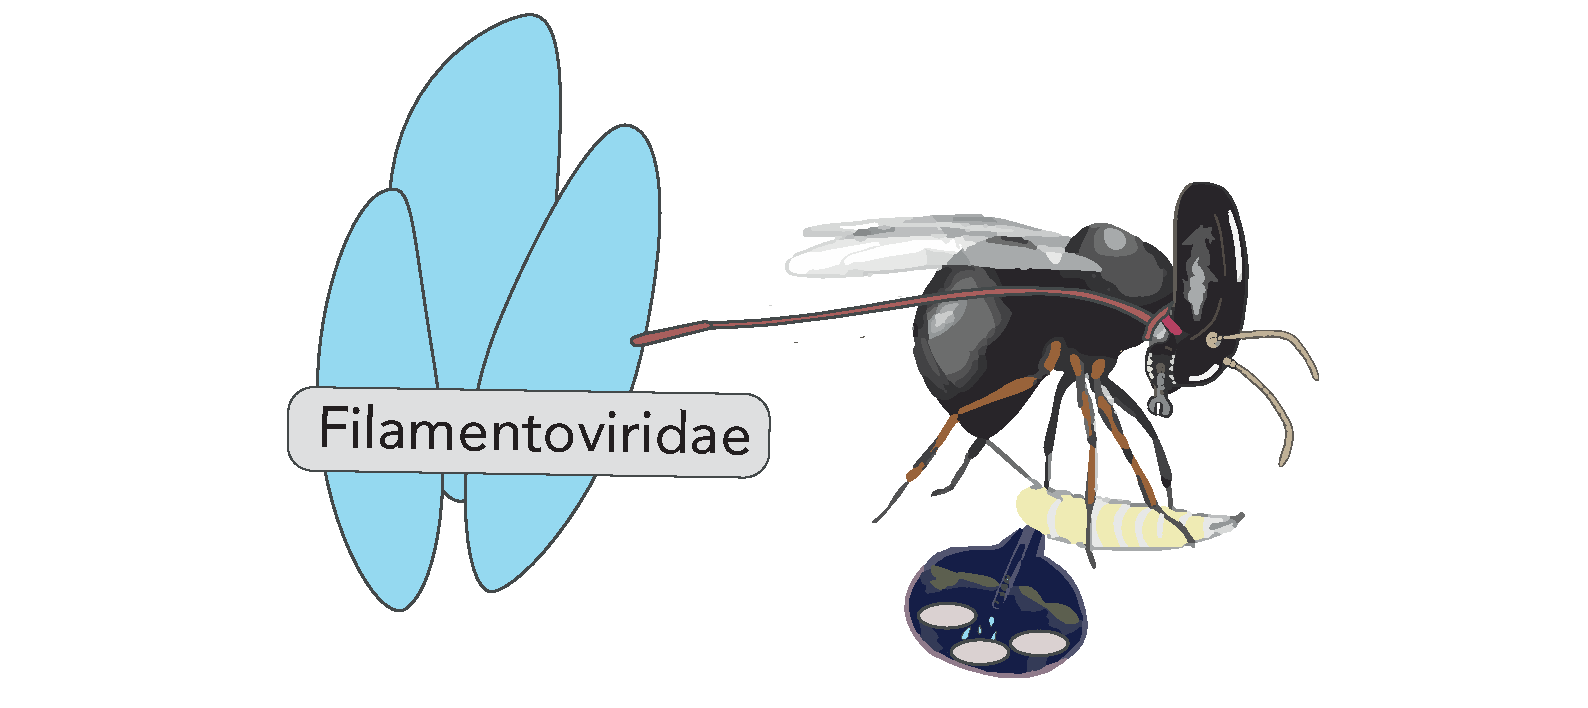
\includegraphics[width=\linewidth,height=\textheight,keepaspectratio]{PhD-master/figures/Manipulation_illustration_Eucoilini.pdf}
\label{figure:Manipulation_illustration_Eucoilini}
\end{figure}

LbFV qui fait partie de la famille des Filamentoviridae a un fort impact sur le comportement de ponte de son hôte \textit{L.boulardi}. Dans ce cas, les femelles infectées par LbFV acceptent facilement de pondre leurs œufs dans des hôtes déjà parasités, contrairement aux femelles non infectées \citep{varaldi_infectious_2003,varaldi_artifical_2006}. Cette induction de "superparasitisme" permet la transmission horizontale du virus dans la population, augmentant ainsi sa valeur sélective au détriment de celle des guêpes \citep{gandon_superparasitism_2006}. Une question ouverte est de savoir si cette manipulation comportementale pourrait être un trait partagé par certains ou tous les membres de Filamentoviridae. Une étude précédente a recherché les gènes LbFV impliqués dans la manipulation du comportement de ponte de \textit{L. boulardi} \citep{varaldi_deciphering_2018}. Le raisonnement de cette étude était qu'un transcrit viral impliqué dans la manipulation du comportement (effecteur) devait (i) être présent chez les femelles adultes, car c'est là et au moment où la manipulation a lieu, et (ii) avoir une abondance biaisée vers l'abdomen (s'il agit sur la prise d'information) ou (iii) vers la tête (s'il agit sur le traitement de l'information dans le système nerveux central). 
Ainsi, la liste des candidats exclut les transcrits viraux qui ne seraient pas présents chez la femelle adulte ou qui seraient d'une abondance similaire dans les deux tissus (comme les inhibiteurs apoptotiques). Aussi, dans cette étude transcriptomique, l'abdomen et la tête de \textit{L. boulardi} ont exprimé 20 ORFs différemment en présence du virus \citep{varaldi_deciphering_2018}. Deux de ces 20 gènes candidats de manipulation du comportement correspondent selon nos analyses de \hyperref[sec:chap2]{chapitre 2} à des gènes cœurs spécifiques des Filamentoviridae (LbFV\_orf94 et LbFV\_orf37 (\textit{Ac38})). Bien que ces gènes ne soient que des candidats impliqués dans la manipulation du comportement chez LbFV, cela ouvre la possibilité qu'ils puissent être impliqués dans la manipulation du comportement chez tous les Filamentoviridae. Si cela s'avère être le cas, la manipulation du comportement de ponte des espèces endoparasitoïdes que ces virus semblent infecter spécifiquement pourrait avoir été une étape évolutive majeure pour ces virus, leur permettant de se spécialiser dans ce mode de vie et de transmettre plus efficacement pendant les événements de ponte. Néanmoins, il est clair que des données phénotypiques supplémentaires et des tests fonctionnels avec d'autres guêpes infectées seront nécessaires pour évaluer cette hypothèse. 

\section{Conclusion générale}

En conclusion, cette thèse avait pour objectif d'évaluer l'importance des virus dans l'évolution des espèces de guêpes endoparasitoïdes. En étudiant l'endogénisation et la domestication des virus chez les Hyménoptères, nous avons montré que l'endoparasitoïdisme pouvait être une stratégie de vie favorisant l'intégration et la domestication des virus à ADN double brins, ce qui semble en partie expliqué par l'évolution de la production de particules à allure virales dans un contexte de forte exposition au système immunitaire de l'hôte. Nous avons également identifié une nouvelle famille de virus à ADN grâce à l'analyse de données exogènes provenant des séquençages d'Hyménoptères. Ces résultats sont très encourageants et nous permettent d'envisager de futures analyses systématiques de ce type, qui pourraient conduire à la découverte d'autres virus à ADN dissimulés dans les assemblages de génomes. Dans la section qui suit la conclusion, je propose quelques exemples et suggestions de méthodes pour analyser ce genre de données à grande échelle. Dans le \hyperref[sec:chap2]{chapitre 2}, nous avons pu ainsi décrire de nouveaux virus à allure filamenteuse, dont nous pensons que les espèces forment une nouvelle famille que nous proposons de nommer les Filamentoviridae. Nous avons également vu que ces virus étaient présents essentiellement chez des espèces de guêpes endoparasitoïdes, profitant certainement des particularités  liées à ce mode de vie. Enfin, nous avons précisé un événement majeur de domestication virale qui s'est produit il y a environ 75 millions d'années dans un clade de guêpes endoparasitoïdes de la tribu des Eucoilini, dont nous pensons que l'évènement de domestication a pu participer à la radiation de ce groupe de guêpe. Ainsi, ce travail dans sa globalité permet de mieux comprendre l'histoire évolutive des virus à ADN double brins et leurs liens privilégiés avec les guêpes au mode de vie endoparasitoïdes. À l'avenir, la recherche de domestication virale pourrait être étendue à d'autres espèces ayant un mode de vie similaire, comme les espèces de diptère parasitoïdes qui sont soumises aux mêmes pressions évolutives. Enfin, l'implication des Filamentoviridae dans la biologie des Eucoilini soulève également la question de leur implication dans la biologie d'autres espèces endoparasitoïdes puisqu'il semble que ces virus soient associés à de nombreuses espèces présentant ce style de vie. Les recherches futures dans ce domaine, analysant la capacité de ces virus à manipuler les comportements de ponte ou bien la caractérisation d'autres évènements de domestication intra-génomique les concernant, seront très certainement des travaux stimulants. 


%Brouillon 


%\textit{Integration non-aléatoire des EVEs} #plutôt en discussion

%De manière générale, le nombre d'EVE semble corrélé à la taille des génomes. Une méta-analyse à l'échelle des insectes montre par exemple une forte corrélation positive \cite{Gilbert 2022} entre le nombre d'EVEs et la taille des 37 génomes. Ces observations font echo à ce qui est retrouvé concernant les éléments transposables (ETs) et d'autres éléments répétés (Lower SS, Johnston et al 2017, Sessegolo C 2016). À la suite de ces observations, nous pouvons émettre l'hypothèse que les EVEs, tout comme les ETs puissent être présents dans des régions avec une densité en gène réduite où la sélection purifiante serait moins élevée. À la suite de notre analyse à l'échelle de 124 génomes d'espèces Hyménoptères, nous avons par exemple pu constater que la probabilité d'observer un élément répété autour d'un gène très conservé (BUSCO) était significativement plus faible comparé à la probabilité d'observer un élément répété dans une région prise aléatoirement dans le génome (voir figurex). De plus, nous avons également observé que la probabilité d'observer un élément répété aux alentours d'un EVE (provenant de virus ARN ou ADN) est significativement plus grande comparée à des gènes BUSCO, et en revanche significativement identique à une région aléatoire du génome. Ces résultats, bien que nécessitant des approches plus robustes de recherche exhaustives des ETs tendant à soutenir l'hypothèse selon laquelle les EVEs seraient présents dans des régions du génome moins contraintes par la sélection. Ce qui a du sens si on imagine que la majorité des insertions accidentelle devraient être contre-sélectionnées, alors seulement les régions faiblement contraintes devraient  toujours porter ces EVEs. 




%\subsection{Le biais de la recherche de domestication virale prédisposant à la production de VLS}

%Bien que les cas de domestication décrits jusqu'à présents concernent des milliers d'espèces de guêpes, ils ne représentent qu'une petite partie de l'immense diversité des Hyménoptères. En outre, ils appartiennent principalement tous à la même super-famille (Ichneumonoidea), ce qui implique un biais dans l'effort d'échantillonnage au sein de la diversité des hyménoptères parasitoïdes. Avec notre étude du chapitre1 sur une plus large échelle de 124 espèces regroupant 12 super-familles d'Hyménoptères, nous n'approchons qu'à peine cette diversité et les résultats nous montrent qu'un seul nouveau cas convaincant au sein de la superfamille des Platygastroïdae, représentée par seulement deux genres de notre jeu de donnée (4 espèces). 

%Par ailleurs, d'autres taxons d'insectes, tels que les Tachinidae (Diptères), ou des Carabidae (Coléoptères) ont évolué de manière indépendante vers le parasitoïdisme, mais nous ne savons rien de leurs interactions avec les virus.

%Avec l'apport de nouveaux génomes presque journalier, il sera ainsi possible de proposer dans le futur des projets qui élargissent notre compréhension des virus et de leur domestication chez les parasitoïdes. À cette fin, des efforts de séquençage pourraient être réalisés sur des superfamilles sous-représentées dans les bases de données et présentant pourtant des schémas de radiation proches de ceux retrouvés chez les Eucoilini ou bien les Microgastroïdes. 

%Par exemple, comme les Ichneumonoidea qui comportent près de 100 000 espèces \citep{10.1146/annurev.ento.51.110104.151029}, pour lesquels la majorité des cas de domestication de virus sont connus, les Chalcidoidea comprennent 22,500 espèces décrites pour une estimation de 500 000 espèces \citep{10.1016/j.ympev.2017.12.005,10.1111/j.1365-3113.1984.tb00056.x}. Des recherches récentes suggèrent que les Chalcidoidea ont d'abord divergé entre 129 et 81 millions d'années (mya), puisque la plupart des lignées existantes ont rapidement divergé à nouveau entre 75 et 53 mya \citep{10.1016/j.ympev.2017.12.005}. Dans notre analyse, nous avons enrichi le jeu de donnée pour cette superfamille avec l'apport de 33 espèces représentant 16 genres et 9 familles pour une superfamille composé de 22 familles décrites \citep{https://doi.org/10.1111/cla.12006}. Malgré tout, nous n'avons observé aucun évènement de domestication viral impliquant la production de VLS. Cependant, parmi l'ensemble de ces 33 espèces, seulement 8 correspondaient à des espèces endoparasitoïdes. Aussi, si on en croit nos observations, ce type d'évènement de domestication devrait principalement se retrouver chez des espèces endoparasitoïdes. Il serait donc intéressant de sonder plus en profondeur cette superfamille en incluant plus d'espèces endoparasitoïdes comme provenant des Encyrtidae (principalement endoparasitoïdes), des Eulophidae (Entedoninae : Euderomphalini) (endoparasitoïdes) ou bien des espèces endoparasitoïdes de la lignée des aphelinides-trichogrammatides. De plus, ce clade est intéressant pour améliorer le test de l'effet du style de vie sur la capacité à endogéniser et/ou domestiquer des éléments viraux puisque celle superfamille contient de nombreux évènements de retour à la vie libre.


%\subsection{Le biais de la recherche de domestication lié à un faible échantillonnage de la diversité virale}

%La recherche d'éléments viraux domestiqués et donc la recherche d'homologie virale dans les bases de données est directement liée à la diversité des séquences virales disponibles dans les bases de données. À titre d'exemple, chez les espèces \textit{Hyposoter. sp}, \textit{Campoletis. sp},  et \textit{Casinaria. sp}  correspondant à un évènement chez les Campopleginae et les espèces \textit{Lyssonata. sp}, \textit{Meniscomorpha. sp}, \textit{Australoglypta. sp} et  \textit{Glypta. sp} correspondant à un évènement chez les Banchinae, le virus domestiqué est inconnu, soit, car sa lignée s'est éteinte, soit, car aucun virus circulant suffisamment proche n'a encore été séquencé \citep{volkoff_analysis_2010, beliveau_genomic_2015}. Dans tous les cas, les analyses basées uniquement sur l'homologie des séquences, telles que celles menées au chapitre 1, ne permettront pas de détecter de tels événements. Ainsi, compte tenu de la diversité des virus séquencés, de tels évènements qui ne pourront jamais être détectés par des approches d'homologies de séquences devraient correspondre à une proportion importante des évènements existants.

%Cependant, parfois un séquençage, même partiel, du paysage de la diversité virale, peut être suffisant pour détecter des événements de domestication impliquant plusieurs gènes. En effet, si nous utilisons les Eucoilini du chapitre 3 comme exemple, nous pouvons constater que le virus qui s'est intégré il y a environ 75 millions d'années appartient à une famille que nous avons décrite au chapitre 2 : les Filamentoviridae. Même après avoir retiré tous les Filamentoviridae de la base de données, dix gènes domestiqués sur quinze présentent des homologies de séquence avec des ORFs de virus n'appartenant pas à cette famille. Ces résultats suggèrent que lorsqu'un gène est domestiqué, il tend à être fortement contraint par la sélection et, par conséquent, accumule moins de changements au niveau des acides aminés, ce qui le rend plus facile à détecter par homologie de séquence. En outre, il semble que dans la majorité des cas connus, les gènes les plus conservés également au niveau viral (les gènes cœurs) sont typiquement ceux qui sont domestiqués chez les endoparasitoïdes. Ceci est probablement dû au fait que ces gènes sont également essentiels à la production de particules virales.

%Ainsi, il apparaît que le séquençage dans un ordre viral tel que les \textit{Lefavirales} devrait permettre d'observer tous les événements impliquant la domestication d'un virus de cet ordre. Par conséquent, dans le cas des ichnovirus, les deux virus impliqués semblent être relativement éloignés de ceux retrouvés dans le clade \textit{Lefavirales}, en tout cas assez divergents pour ne plus retrouver de trace d'homologie de séquences. 





%paler du fait que les filamenteux ont laissé des traces d'endogénisation chez beaucoup d'espèces et que pour le coup c'est le signe qu'ils ont ou infectent une large gamme d'hôte, surtout des endoparasitoïdes, ce qui permet sans doute un apport conséquent en gènes pouvant mener à de la domestication


%Jusqu'en 2017 aucun génome viral de virus filamenteux n'était disponible dans les bases de données \citep{lepetit_genome_2017}. Un an après son séquençage, des premières évidences montrent la domestication d'un virus filamenteux impliquant la production de VLPs chez les \textit{Leptopilina}(Di Giovanni et al., 2020). Grâce aux apports du chapitre 3, nous avons pu voir que cet événement implique probablement un grand nombre d'espèces puisque l'évènement d'endogénisation s'est produit il y a 75 millions d'années et concerne au moins 4 genres analysés dans la diversité des Eucoilini. Dans le chapitre 2, nous avons voulu screener 



%\section{Dater les phylogénies virales à l'aide de EVEs : un processus compliqué}

%\section{La domestication virale chez d'autres insectes parasitoïdes}



%\section{La bio-informatique ne se suffit pas à elle-même pour décrire de la domestication moléculaire}







    \part{Études}
    \thispagestyle{empty}
    \chapter{Endoparasitoid lifestyle promotes endogenization and domestication of dsDNA viruses}
    \label{chap:Domestication_within_parasitoids}

    \begin{center}
        \Large Benjamin guinet$^{\text{1}}$, David Lepetit$^{\text{1}}$, David G Notton$^{\text{7}}$, Elijah J Talamas$^{\text{8}}$, Jean-Yves Rasplus$^{\text{2}}$, Julia Stigenberg$^{\text{5}}$ , Lene Sigsgaard$^{\text{3}}$, Nicolas Ris$^{\text{4}}$, Peter N$^{\text{6}}$, Sylvain Charlat$^{\text{1}}$, Damien de Vienne$^{\text{1}}$, Bastien Boussau$^{\text{1}}$, Julien Varaldi$^{\text{1}}$\\
        \vspace{0.5cm}
        \scriptsize
        $^{\text{1}}${Université Lyon 1, CNRS, Laboratoire de Biométrie et Biologie Evolutive UMR 5558, F-69622 Villeurbanne, France.}\\
        $^{\text{2}}${INRA, UMR1062 CBGP, F-34988 Montferrier-sur-Lez, France.}\\
        $^{\text{3}}${Department of Plant and Environmental Sciences, University of Copenhagen, Thorvaldsensvej 40, 1871 Frederiksberg C, Denmark.}\\
        $^{\text{4}}${INRAE, Institut Sophia-Agrobiotech, Université Côte d'Azur, CNRS, 06903 Sophia Antipolis, France.}\\
        $^{\text{5}}${Department of Zoology, Swedish Museum of Natural History, Box 50007, 104 05 Stockholm, Sweden.}\\
        $^{\text{6}}${Zoological Museum, Department of Entomology, University of Copenhagen,
        Universitet sparken 15, DK-2100 Copenhagen, Denmark.}\\
        $^{\text{7}}${Natural Sciences Department, National Museums Collection Centre, 242 West Granton Road, Granton, Edinburgh, EH5 1JA, United Kingdom.}\\
        $^{\text{8}}${Department of Plant Industry, Florida Department of Agriculture and Consumer Services, Gainesville, FL 32399, USA.}\\
    \end{center}
     \setcounter{minitocdepth}{1}

    {\hypersetup{linkcolor=GREYDARK}\minitoc}
\clearpage

\label{sec:chap1}

\section{Reproducibility and Supplemental material}
All additional scripts and large figures are available at the following GitHub link : \newline (\href{https://github.com/BenjaminGuinet/PhD_defense/tree/main/Supplementary_paper1}{Supplementary\_paper1}).

\section{Abstract}

The accidental endogenization of viral elements within eukaryotic genomes can occasionally provide significant evolutionary benefits, giving rise to their long-term retention, that is, to viral domestication. For instance, in some endoparasitoid wasps (whose immature stages develop inside their hosts), the membrane-fusion property of double-stranded DNA viruses has been repeatedly domesticated following ancestral
endogenizations. The endogenized genes provide female wasps with a delivery tool to inject virulence factors that are essential to the developmental success of their offspring. Because all known cases of viral domestication involve endoparasitic wasps, we hypothesized that this lifestyle, relying on a close interaction between individuals, may have promoted the endogenization and domestication of viruses. By analyzing the composition of 124 Hymenoptera genomes, spread over the diversity of this clade and including free-living, ecto- and endoparasitoid species, we tested this hypothesis. Our analysis first revealed that double-stranded DNA viruses, in comparisons with other viral genomic structures (ssDNA, dsRNA, ssRNA), are more often endogenized and domesticated (that is, retained by selection) than expected from their estimated abundance in insect viral communities. Secondly, our analysis indicates that the rate at which dsDNA viruses are endogenized is higher in endoparasitoids than in ectoparasitoids or free-living hymenopterans, which also translates into more frequent events of domestication. Hence, these results are consistent with the hypothesis that the endoparasitoid lifestyle has facilitated the endogenization of dsDNA viruses, in turn increasing the opportunities of domestications that now play a central role in the biology of many endoparasitoid lineages.


\section{Introduction}

The recent boom of genome sequencing programs has revealed the abundance of DNA fragments of viral origin within eukaryotic genomes. These so-called Endogenous Viral Elements (EVEs) stem from endogenization events that not only involve retroviruses as donors (as could be expected from their natural lifecycle) but also viruses that do not typically integrate into their host chromosomes \citep{katzourakis_endogenous_2010,feschotte_endogenous_2012,aswad_evolutionary_2021}. In insects, where retroviruses have yet to be found, endogenization events have involved various non-retroviral viruses: three families of large double-stranded (ds) DNA viruses, at least 22 families of RNA viruses, and three families of single-stranded (ss) DNA viruses \citep{gilbert_diversity_2022}. Degeneracy and loss is likely the fate of most EVEs, since they do not \textit{a priori} benefit their hosts. Still, several studies have reported that EVEs can be retained by selection, thus becoming \textit{domesticated} \citep{koonin_depths_2018}. The functions involved include defensive properties against related viruses in mosquitoes \citep{yan_origin_2009,suzuki_non-retroviral_2020}, against macroparasites in some Lepidoptera \citep{gasmi_horizontally_2021}, or modifications in the expression of genes involved in dispersal in aphids \citep{parker_laterally_2019}. Beyond insects, the membrane fusion capacity of viruses, allowing their entry into host cells, has been repeatedly co-opted in three metazoan clades: mammals, viviparous lizards and parasitoid wasps. In placental mammals and viviparous Scincidae lizards, domestication of the \textit{syncytin} protein from retroviruses has allowed the emergence of the placenta, through the development of the syncytium (composed of fused cells) involved in metabolic exchanges between the mother and the fetus \citep{lavialle_paleovirology_2013,cornelis_endogenous_2017}. A similar fusogenic property was repeatedly co-opted by parasitoids belonging to the Hymenoptera order through the  endogenization and domestication of complex viral machineries deriving from large dsDNA viruses  \citep{drezen_endogenous_2017, gilbert_diversity_2022}. The numerous retained viral genes allow parasitoid wasps to produce virus-like structures (VLS) within their reproductive apparatus. These are injected into the wasp's host, together with their eggs, and protect the wasp progeny against the host immune response. This protection is achieved thanks to the ability of VLS to deliver virulence factors in the form of genes (in which case VLS are called polydnavirus - PDV) or proteins (in which case VLS are called Virus-like particles - VLPs) to host immune cells (reviewed in \citep{gauthier_recurrent_2018, drezen_bracoviruses_2021}). So far, 5 independent cases of such viral domestication have been detected in parasitoid wasps, four of them falling within the Ichneumonoidea superfamily \citep{bezier_polydnaviruses_2009,volkoff_analysis_2010,pichon_recurrent_2015,burke_common_2019} and one in the Cynipoidea superfamily (Di Giovanni et al., 2020). The four cases where the donor virus family has been unequivocally identified point towards dsDNA viruses. More specifically, the domesticated EVEs (hereafter, dEVEs) derive from the \textit{Nudiviridae} family in three cases \citep{bezier_polydnaviruses_2009,pichon_recurrent_2015,burke_common_2019} while the forth involves a putatively new viral family denoted "LbFV-like" (Di Giovanni et al., 2020). Notably, all these domestication events took place in endoparasitoids, that is, in species that deposit their eggs inside the hosts, as opposed to ectoparasitoids that lay on their surface.

Beyond these well characterized events of viral domestication in Hymenoptera, additional cases of endogenization have been uncovered, in studies that enlarged the taxonomic focus of either the hosts \citep{ter_horst_endogenous_2019, cheng_nudivirus_2020,kondo_novel_2019} or the viruses that were considered  \citep{flynn_assessing_2019,ter_horst_endogenous_2019,irwin_systematic_2022,li_hgt_2022}. Here, we complement this earlier work by expanding the range of both the hosts and viruses under study, and by further analyzing which endogenization cases have been followed by a domestication event.

To this end, we developed a bioinformatic pipeline to detect endogenization events involving any kind of viruses (DNA/RNA, single-stranded, double-stranded), at the scale of the whole Hymenoptera order. This analysis first allowed us to test whether the propensity of viruses to enter Hymenoptera genomes, and to be domesticated, depend on their genomic structure (in line with the pattern observed so far, where only dsDNA viruses have been involved in domestication events as described above). 
We then tested whether the lifestyle of the species (free-living, endoparasitoid, ectoparasitoid) correlates with their propensity to integrate and domesticate viruses. Our working hypothesis was that the endoparasitoid lifestyle may be associated with a higher rate of viral endogenization and / or a higher rate of domestication events, for two non-exclusive reasons related either to the exposure  to new viruses and the adaptive value of the endogenized elements.

First, a higher endogenization rate may simply stem from a higher exposure to viruses. Such an effect could be at play in endoparasitoids due to the intimate interaction between the parasitoid egg or larva and the host.  In other words, the endo-parasitic way of life may facilitate the acquisition of new viruses deriving from the hosts. Notably, this lifestyle may also facilitate the maintenance and spread of newly acquired viruses within wasp populations. Indeed, endoparasitoid wasps often inject not only eggs but also venomic compounds (typically produced in the venom gland or in calyx cells) where viruses can be present and may thus be vertically transmitted \citep{martinez_additional_2016}).  In addition, the confinement of the several  developing wasps within a single host may facilitate viral horizontal transmission  and its subsequent spread in wasps populations (e.g. \citep{varaldi_infectious_2003}).

Second, a higher rate of domestication in endoparasitoids may be the consequence of a particular selective regime. This is expected since, these insects are facing the very special challenge of resisting the host immune system, contrary to other lifestyles. This selective pressure may promote the co-option of viral functions such as the above-mentioned membrane fusion activity, that provide a very effective mean to deliver virulence factors. 

Our analysis reveals numerous new instances of endogenization events, some of which are also characterized by signatures of molecular domestication. We found a clear enrichment in endogenization events deriving from dsDNA viruses as compared to those with other genomic structures. While the data did not reveal a significant effect of Hymenoptera lifestyles on the acquisition of dsRNA, ssRNA or ssDNA viruses, it supports the hypothesis that genes from dsDNA viruses are more often endogenized and domesticated in endoparasitoids than in free-living and ectoparasitoid species.

%\end{multicols}

\afterpage{%
\onecolumn
\begin{figure}[!htpb]
\captionsetup{font=footnotesize}
 \centering
  \includegraphics[width=\linewidth,height=\textheight,keepaspectratio]{PhD-master/figures/Main_phylogeny_figure2.pdf}
\caption[Paper1:EVE distribution along the Hymenoptera phylogeny]{\textbf{Endogenous Viral Elements and their domestication status in Hymenoptera. }
Lifestyles are displayed next to species names (blue: free-living, green: endoparasitoid, yellow: ectoparasitoid, grey: unknown). The number of EVEs and domesticated EVEs (dEVEs) found in each species are represented respectively by the first and second facet of the horizontal histograms. Colors along these histograms indicate the potential donor viral families (where blue tones correspond to viral dsDNA viruses, red tones to ssDNA viruses, orange/brown tones to dsRNA viruses and green tones to ssRNA genomes). Endogenous Viral elements (EVEs) shared by multiple species and classified within the same event are represented by circles whose size is proportional to their number; those that are considered as domesticated (dEVEs) are surrounded by a black border. Numbers in the white boxes correspond to the number of endogenization events inferred. As an example, \textit{Megastigmus dorsalis} and \textit{Megastigmus stigmatizans} are ectoparasitoids (yellow) sharing a common endogenization event (within the Cluster21304) that likely originated from an unclassified dsRNA virus (grey color in circle), and shows no sign of domestication (no black border around the grey part of the circle). The figure was inspired from the work of \citep{peters_evolutionary_2017}. Details on the phylogenetic inference and time calibration can be found in the Materiel and Methods section; bootstrap information can be found in \tablename{\ref{tab:Summary_candidate_numbers}}; details on lifestyle assignation can be found on the GitHub file : \href{https://github.com/BenjaminGuinet/PhD_defense/blob/main/Supplementary_paper1/Assembly_genome_informations.csv}{Assembly\_genome\_informations.csv}.}
\label{figure:Event_phylogeny}
\end{figure}

\clearpage
}

\section{Results}

We screened for EVEs 124 Hymenoptera genome assemblies, including 24 ectoparasitoids, 37 endoparasitoids and 63 free-living species (the list can be found on the GitHub file : \href{https://github.com/BenjaminGuinet/PhD_defense/blob/main/Supplementary_paper1/Assembly_genome_informations.csv}{Assembly\_genome\_informations.csv}). EVEs were identified using a sequence-homology approach based on a comprehensive viral protein database. Different confidence levels (ranging from A to D) were associated with the various EVEs inferred, where the A score indicates a maximal confidence level for endogenization. This confidence index is based upon sequencing depth combined with the presence of eukaryotic genes and/or transposable elements in the genomic environment of the candidate loci (as detailed in the Material and Methods section). By default, the four categories are included in the analysis, but unless otherwise stated statistical tests based on the A category only led to the same conclusions (see \figurename{\ref{figure:Bioinformatic_pipeline}}-7 for more details). Our analysis further included an inference of the phylogenetic relationships among homologous EVEs, that was used to map endogenization events on the Hymenoptera species tree. Finally, inferences of domestication events relied upon signatures of purifying selection in the integrated genes (based on \textit{dN/dS} estimates) and/or on expression data.

An important objective of our analysis is to detect and enumerate not only endogenous viral elements (EVEs) but also endogenization \textit{events} that can explain the presence of these EVEs. Indeed, an EVE denotes a single gene of viral origin in a single species. Several neighboring EVEs in a genome most likely result from the endogenization of a single viral genome, and  homologous EVEs shared by several closely related species may further stem from a single ancestral endogenization events. This distinction is critical when it comes to examining the effect of various factors on the probability of integrating EVEs, which implies counting events rather than EVEs. As an example, consider the \textit{Leptopilina} case  (Di Giovanni et al., 2020), involving 13 EVEs shared by 3 closely related species. In this wasp genus, based on previous findings, we expect the 39 EVEs to be grouped into a single endogenization event. Our pipeline appropriately detected 36 EVEs (out of 39) and correctly aggregated them into a single endogenization event mapped on the branch leading to the \textit{Leptopilina} genus. Furthermore, because some of the genes involved are inferred as domesticated, this event is appropriately classified as a domestication event (see \figurename{ \ref{figure:Event_phylogeny}} and \figurename{ \ref{figure:Event_assignation_examples}} for more canonical examples).  
In total, the pipeline correctly detected 88.4\% (152/172) of the EVEs involved in our four "positive controls", previously described as mediating the protection of young wasps  against their host immune system. Among them, 71.82\% were inferred as being domesticated. Out of the 152 positive controls EVEs, 147  were grouped into 4 independent endogenization events, as was expected. The remaining 5 genes had peculiar histories that led our pipeline to infer two additional spurious events (\tablename{\ref{tab:Control_table}}). All detailed results regarding EVEs and dEVEs can be found on the GitHub file : \href{https://github.com/BenjaminGuinet/PhD_defense/blob/main/Supplementary_paper1/All_EVEs_dEVEs_informations.txt}{All\_EVEs\_dEVEs\_informations.txt}.

\subsection{Endogenizations involve all viral genomic structures}

A total of 1261 EVEs have been inferred in the whole dataset (\tablename{\ref{tab:Summary_candidate_numbers}},\figurename{\ref{figure:Event_phylogeny}}). These come from 367 endogenization events, the majority of which involved ssRNA and dsDNA viruses (41\% and 35\%, respectively) (\tablename{\ref{tab:Summary_candidate_numbers}}). Among the tip branches leading to the 124 species under study, 113 underwent one endogenization event, with a maximum of 14 events and a median of 3 (\figurename{\ref{figure:Event_phylogeny}}). In total, 91\% of the events (331) occurred on tip branches, and the remaining 9\% are shared by at least two closely related species (\tablename{\ref{tab:Summary_candidate_numbers}}, \figurename{\ref{figure:Event_phylogeny}}). To assess the validity of the procedure used to aggregate multiple EVEs into a single shared ancestral endogenization, we assessed whether EVEs inferred as homologous shared a common genomic environment. We thus tested for the presence of homologous loci in descendant species around the shared ancestral EVEs (using blastn searches between the corresponding scaffolds, see details in \hyperref[sec:MM-6]{Materials and methods}). Among the 36 endogenization events that involved at least two species, 31 were found to carry more homologous loci around the insertion sites than expected by chance (see details in \hyperref[sec:MM-6]{Materials and methods}). Notably, the majority of endogenization events involved a single EVE (a single gene) and only 12 (all from dsDNA viruses), involved the concomitant integration of more than 4 viral genes (\figurename{\ref{figure:Genomic_structure_and_families_Events_distributions}}-C).  

A total of 40 different viral clades (usually families) were inferred as putative donors. Most of them (34) are known to infect insects (\figurename{\ref{figure:Genomic_structure_and_families_Events_distributions}}-B) and these account for the majority of the 331 endogenization events.  However, we found 36 EVEs (24 endogenization events), including 20 high-confidence ones (A-ranked), that derived from 6 viral families not previously reported to infect insects (\textit{Phycodnaviridae}, \textit{Herpesviridae}, \textit{Caulimoviridae}, \textit{Asfaviridae}, \textit{Bornaviridae} and \textit{Mypoviridae}). However, in those cases, the true viral donors may belong to unknown clades that do infect insects. Indeed, although the homology with viral proteins was convincing (median e-value was 9.4095e-12 [min = 9.212e-129, max = 3.305e-08]), the average percentage identity was relatively low (38\% [min = 23.2\%, max = 79.1\%], suggesting that these loci may originate from unknown viruses that are only distantly related to their closest relatives in public databases.


\begin{figure}[!htbp]
 \centering
  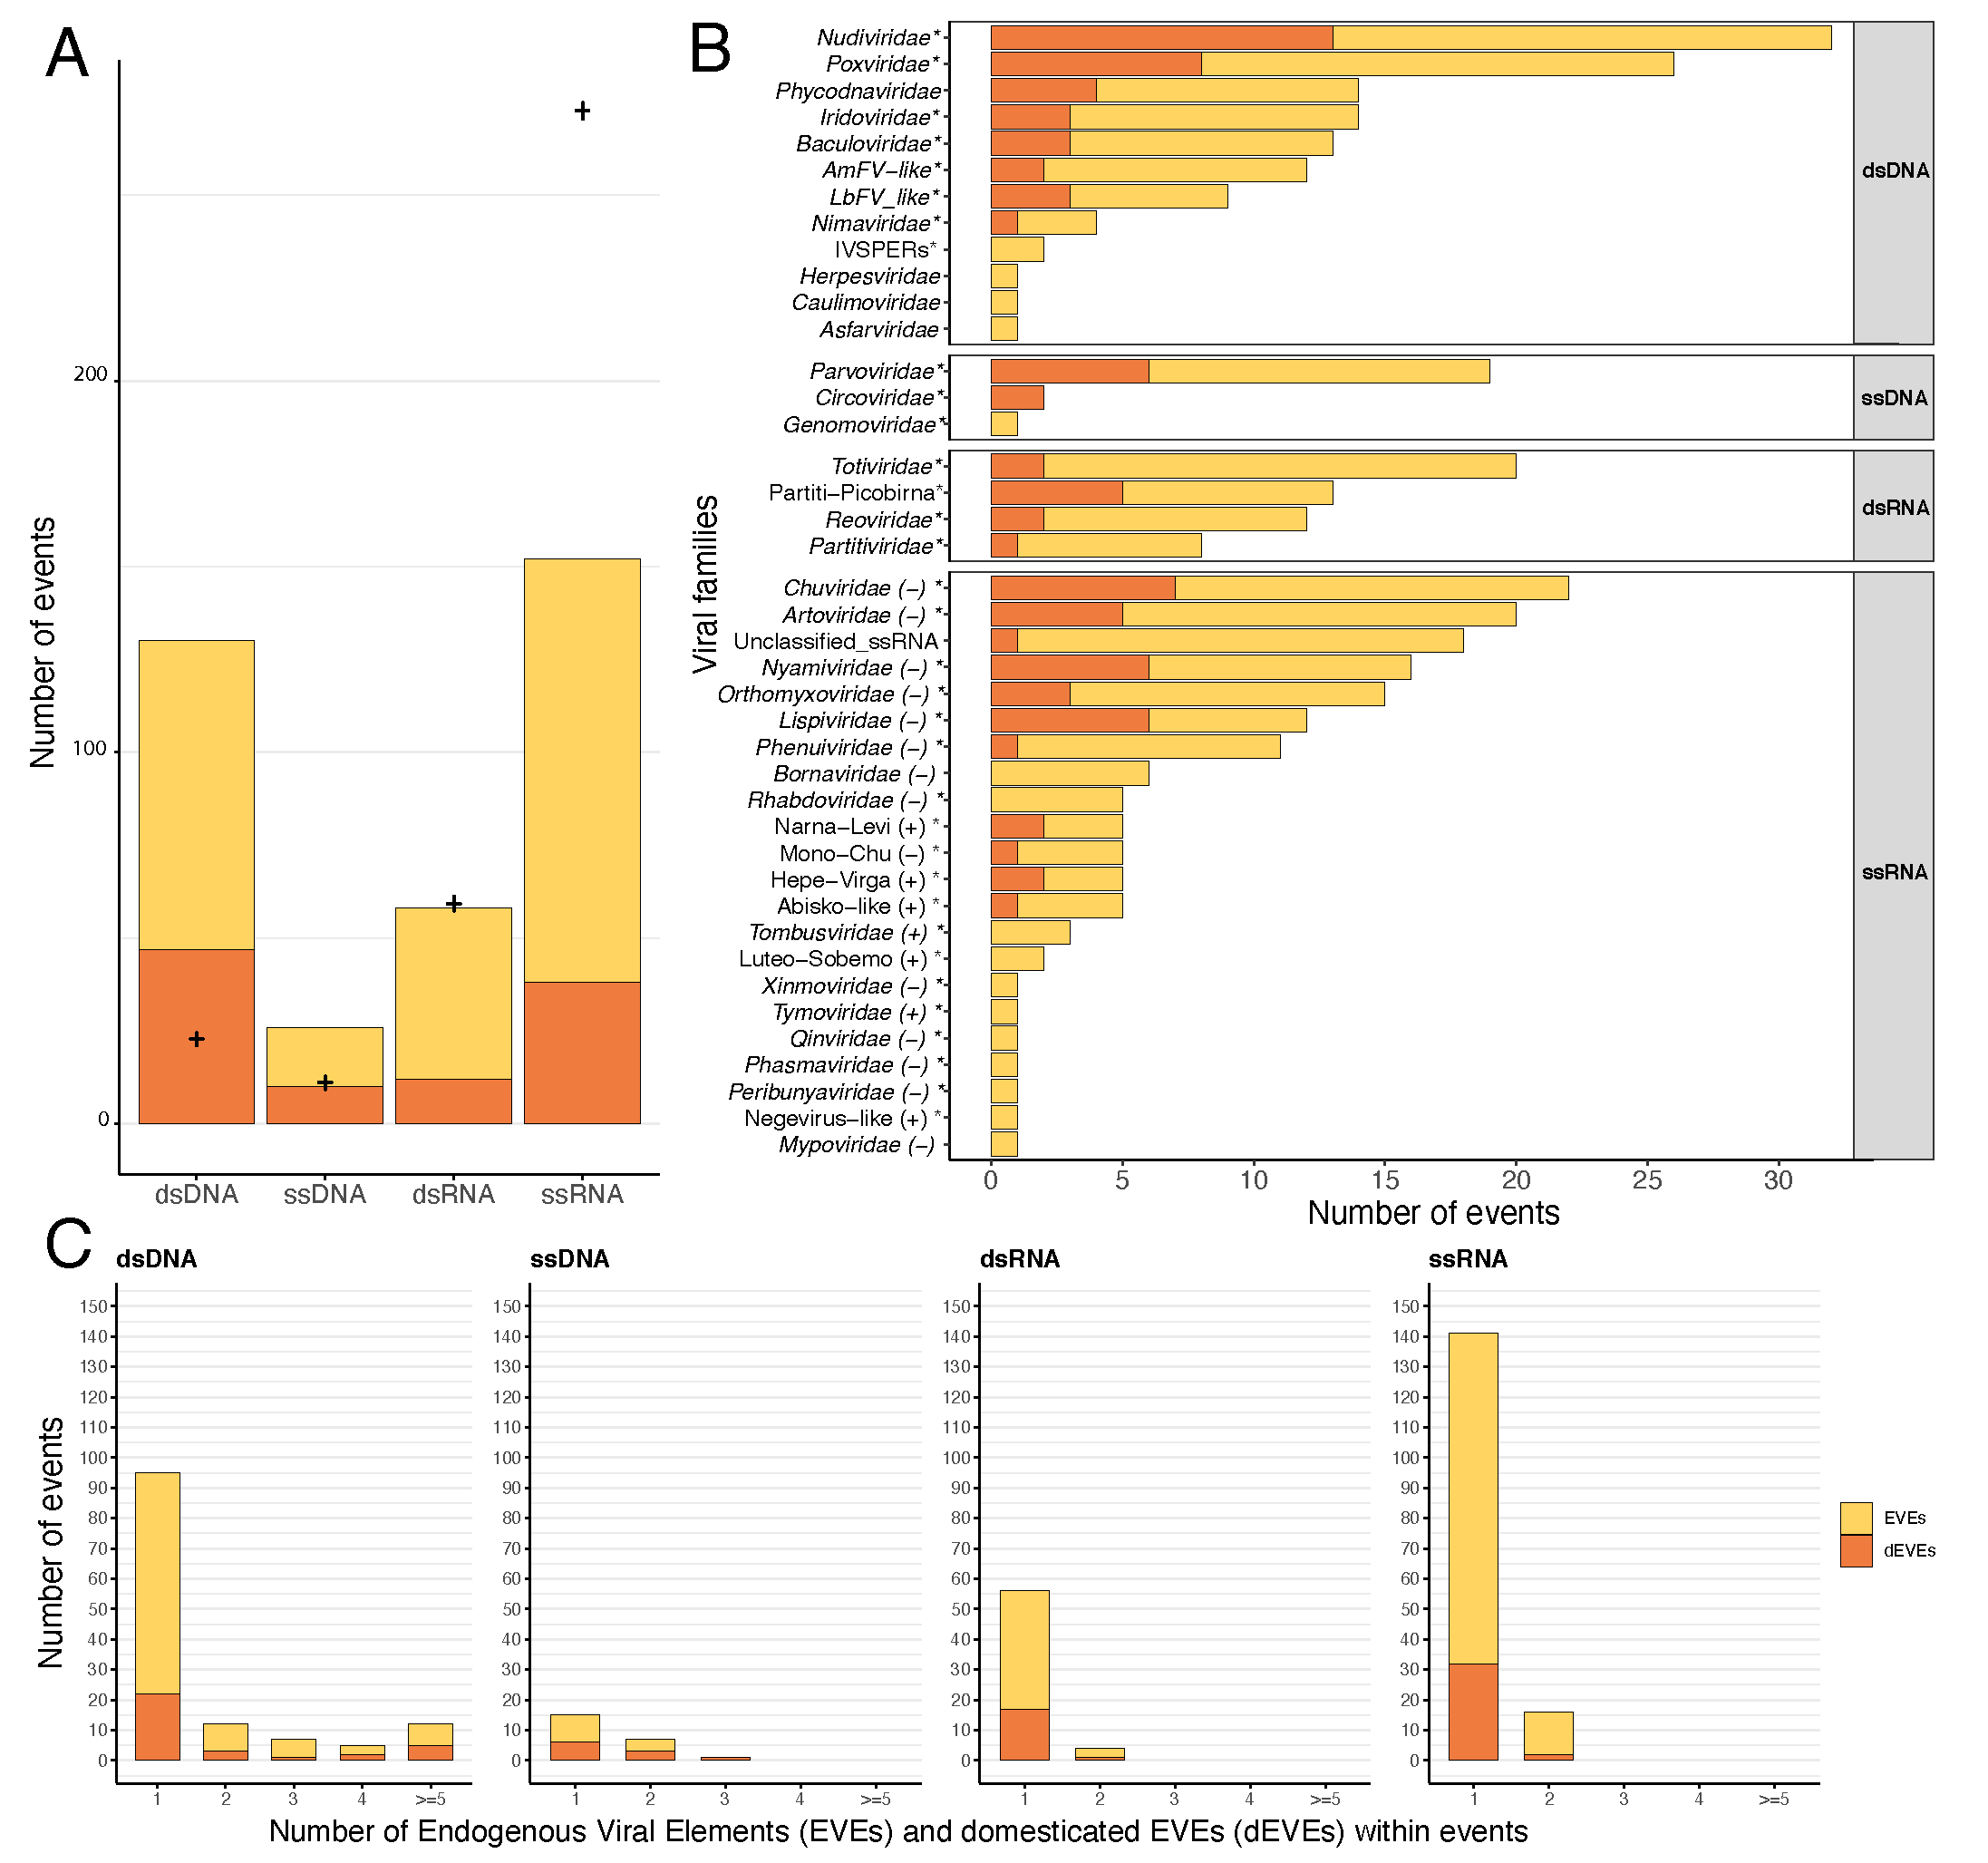
\includegraphics[width=\linewidth,height=\textheight,keepaspectratio]{PhD-master/figures/Genomic_structure_and_families_Events_distributions.pdf}
\caption[Paper1:Distribution of Events and dEvents among viral genomic structures and viral families]{\textbf{Endogenization involves all types of viral genomic structures.} In all three panels, a yellow color indicates endogenization events that have not been followed by domestication, while orange indicates domestication events. \textbf{A} : Distribution of the number of events inferred, according to the four categories of viral genomic structures. The crosses refer to the expected number of endogenization events for each category based on its estimated relative abundance in insects (see details in \hyperref[sec:MM-8]{Materials and methods} and virus-infecting data in Excel tab:All\_virus\_infecting\_insects\_informations).  \textbf{B} :  Distribution of the various viral families involved in endogenization events. The polarity of ssRNA viruses  is displayed next to the family name. Events involving multiple putative families (i.e. where several viral families are present in the same scaffold) have been excluded from the count. The star next to the family name indicates that the viral family is known to infect insects. \textbf{\text{C}} : Distribution of the number of EVEs per event across viral categories.}
\label{figure:Genomic_structure_and_families_Events_distributions}
\end{figure}

\subsection{Double-stranded DNA viruses are over-represented in endogenization events}

Most of the endogenization events recorded involve ssRNA and dsDNA viruses. But do these proportions simply mirror the diversity and respective abundances of the different kinds of viruses encountered by insects?  The analysis summarized in (\figurename{\ref{figure:Genomic_structure_and_families_Events_distributions}}-A) (see details in \hyperref[sec:MM-8]{Materials and methods}) indicates this is not the case. More specifically, it shows that dsDNA viruses are more frequently endogenized than expected on the basis of their representation in the databases, while ssRNA viruses are under-represented  ($\chi^2$ = 213.36 and 221.38, respectively, for endogenization events and domestication events, d.f. = 3, both p-value $<$ 2.2e-16). Notably, this result is not purely driven by the presence in our data set of the four positive controls (previously described cases of viral domestication, that all involve dsDNA viruses as donors). Finally, among endogenization events involving ssRNA viruses, we found an over-representation of negative stranded ssRNA compared to their relative abundance in public databases (72.2\% compared to 32.6\% in the databases, $\chi^2$=145.87, d.f.=1, p-value $<$ 2.2e-16; see \hyperref[sec:SI-1]{supplemental information} for a discussion).\\

\begin{figure}[!htbp]
 \centering
  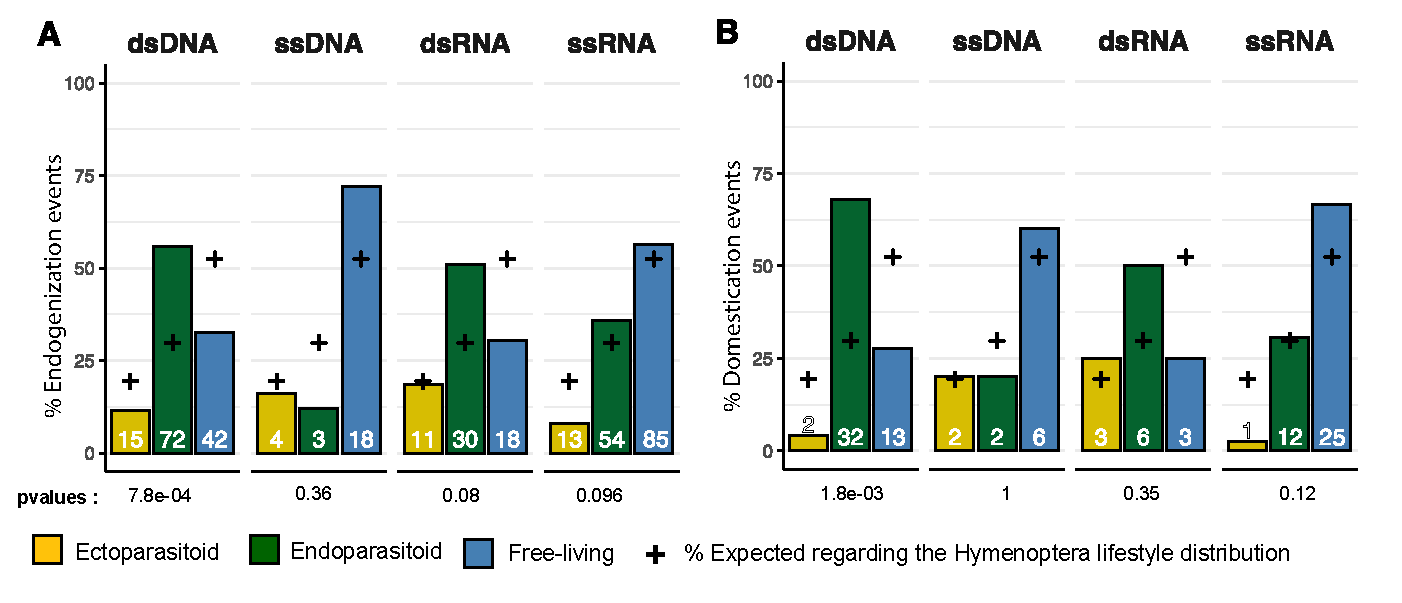
\includegraphics[width=\linewidth,height=\textheight,keepaspectratio]{PhD-master/figures/Lifecycle_Events_per_genomic_structures.pdf}
\caption[Paper1:Distribution of Events and dEvents among viral genomic structures and between lifestyles]{\textbf{Endogenization and domestication of dsDNA viruses are most prevalent in endoparasitoid species}. \textbf{A}: Distribution of viral endogenization events (Event) and  \textbf{B} of domestication events (dEVEs) across Hymenoptera lifestyles.
Crosses indicate the expected proportion of events associated with the different lifestyles, based on the respective frequencies in our database (ectoparasitoid = 24/124, endoparasitoid = 37/124, free-living = 63/124). The p-values are the results of Fisher's tests comparing the observed and expected distributions. Numbers inside the bars indicate the absolute numbers of events inferred. The ancestral states of the nodes, in terms of lifestyle, were inferred in a Bayesian analysis  (see details in \hyperref[sec:MM-5]{Materials and methods})} \label{figure:Lifecycle_Events_per_genomic_structures}.
\end{figure}

\subsection{Endogenizations of dsDNA viruses are more frequent in endoparasitoid species }

Next, we sought to characterize the factors that could explain the patterns of endogenization events inferred (\figurename{\ref{figure:Event_phylogeny}}). To this end, for each viral genomic structure, we assessed whether  endogenization events were evenly distributed among the three wasp lifestyles, taking into account their respective frequencies in the dataset. No significant departure from the null hypothesis was detected for endogenization involving ssDNA, dsRNA or ssRNA viruses (Fisher exact test p-values BH corrected $>$ 0.05). On the contrary, we detected a highly significant enrichment of dsDNA viruses endogenization events in endoparasitoid species, and conversely a deficiency in free-living and ectoparasitoid species (corrected p-value = 7.8e-04, \figurename{ \ref{figure:Lifecycle_Events_per_genomic_structures}-A}). 

To further test the apparent correlation between Hymenoptera lifestyle and the rate of endogenization events, we inferred ancestral lifestyles along the phylogeny using a Bayesian model (see details in  \hyperref[sec:MM-12]{Materials and methods}). We then constructed a generalized linear model where the dependent variable is the number of endogenization events inferred on each branch, while branch length and lifestyle are the explanatory variables (see details in \hyperref[sec:MM-5]{Materials and methods}). Branch length was included as an additive effect to remove the expected effect of time on the number of endogenization events, thus allowing the decomposition of the remaining variance according to the lifestyle (free-living, ectoparasitoid or endoparasitoid).

We first tested whether the rate of endogenization events deriving from any virus (that is, regardless of  their genomic structures) was structured by lifestyles, and found no significant effect (\figurename{ \ref{figure:All_violin_plots}-A left side}). 
We then split the dataset according to the genomic structure of the donor viruses. For RNA or ssDNA virus, the analysis did not reveal evidence of a correlation between wasps' lifestyles and the rate of endogenization events (\figurename{\ref{figure:All_violin_plots}}-G,I and K). On the contrary, in the case of dsDNA viruses, we found a highly significant effect of the wasp lifestyle: endogenization rates appear to be  2.47 times higher in endoparasitoids than in free-living species (89\% CI [1.56-3.56], \figurename{\ref{figure:dsDNA_violin_plot}}-A). The corresponding probability of direction (pd, an index representing the confidence in the direction of an effect) was equal to 99.9\%. In contrast, ectoparasitoids did not differ from free-living species (\figurename{\ref{figure:dsDNA_violin_plot}}-A). Accordingly, more than 98\% of the MCMC iterations led to a higher coefficient value for endoparasitoids than for ectoparasitoids (so-called $P_{MCMC}$ in \figurename{\ref{figure:dsDNA_violin_plot}}-A). This effect was consistently found using high confidence scaffolds only (A-ranked scaffolds, \figurename{\ref{figure:All_violin_plots}}-C right side). We also carried out the same analysis without the 4 domestication cases previously mentioned in the literature (because including them in our data set could have skewed the results) and reached the same conclusion (\figurename{\ref{figure:All_violin_plots}}-E right and left sides). Overall, these results show that dsDNA viruses are more often endogenized in endoparasitoids than in  free-living and ectoparasitoid species.


\begin{figure}[!htbp]
 \centering
  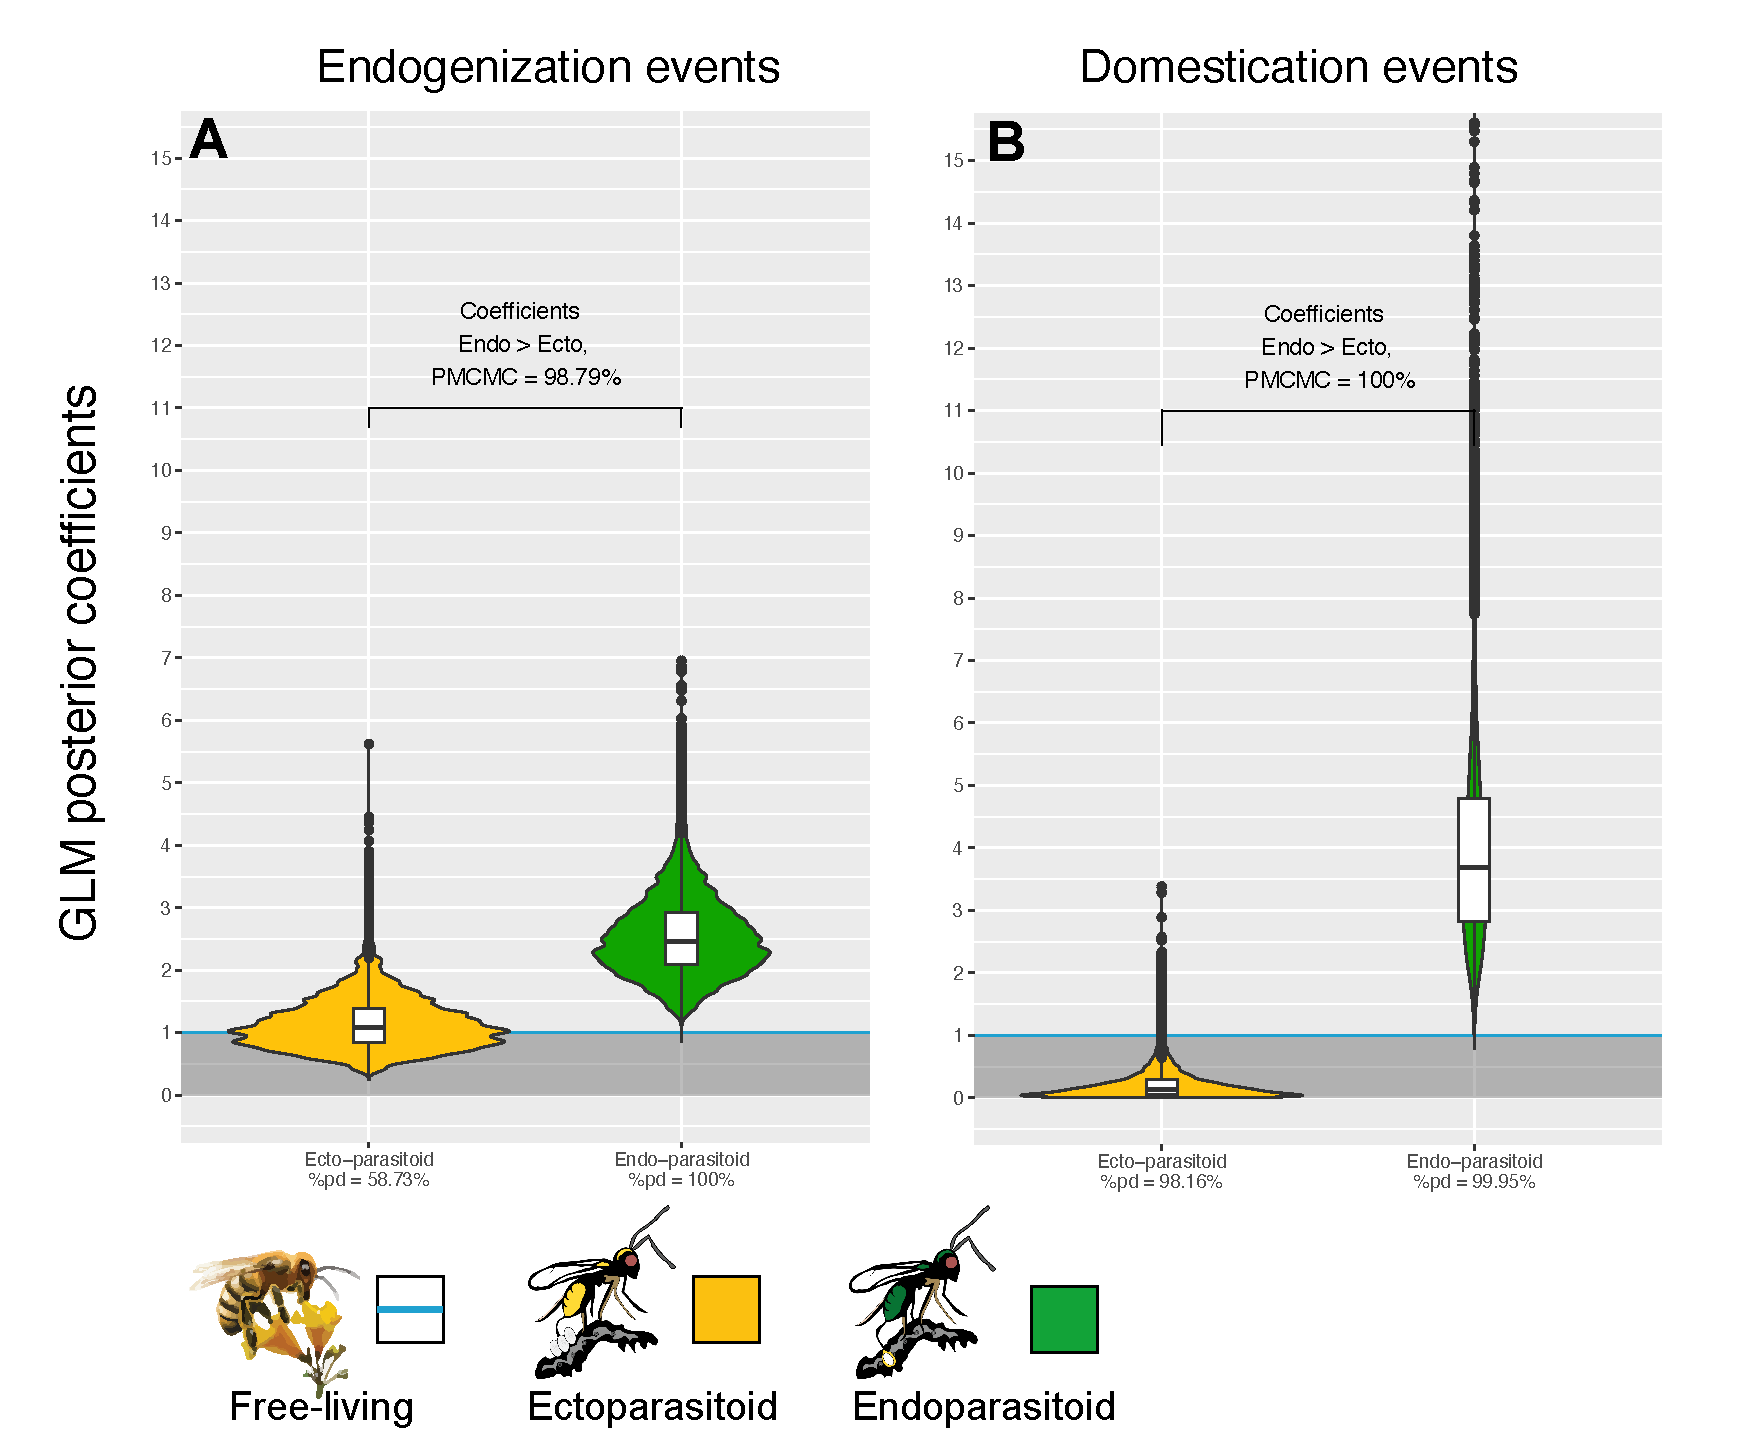
\includegraphics[width=\linewidth,height=\textheight,keepaspectratio]{PhD-master/figures/dsDNA_violin_plots.pdf}
\caption[Paper1:Violin plot GLM coefficients distribution of dsDNA Events and dEvents]{\textbf{Endogenization and domestication of dsDNA viruses are more frequent in endoparasitoid species}. Violin plots represent the posterior distribution of the coefficients obtained under the different GLM models (after exponential transformation to obtain a rate relative to free-living species). The coefficients are derived from 1000 independent GLM models, where 1000 probable scenarios of ancestral states at nodes were sampled randomly among the MCMC iterations (see details in  \hyperref[sec:MM-12]{Materials and methods}). Branches from nodes older than 160 million years were removed from the dataset. The \%pd is the probability of direction and indicates the proportion of the posterior distribution where the coefficients have the same sign as the median coefficient. $P_{MCMC}$ indicates the proportion of MCMC iterations where the coefficient obtained for endoparasitoid species is higher than for ectoparasitoid species. All statistical summaries of the Bayesian GLM models can be found on the GitHub file: \href{https://github.com/BenjaminGuinet/PhD_defense/blob/main/Supplementary_paper1/Lifestyle_statistical_analysis_results.xlsx}{Lifestyle\_statistical\_analysis\_results.xlsx}.}
\label{figure:dsDNA_violin_plot}
\end{figure}

\subsection{Domestications of dsDNA viruses are most prevalent in endoparasitoid species}

We then investigated whether lifestyles may explain the abundance of domestication events. A simple Fisher's exact test approach revealed an enrichment in endoparasitoid species of domestication events involving dsDNA viruses (Benjamini-Hochberg adjusted p-value = 1.8e-03), whereas no deviation from the null hypothesis was detected for the other viral genomic structures (\figurename{ \ref{figure:Lifecycle_Events_per_genomic_structures}-B}).

We built upon the generalized linear models described above, in a Bayesian framework, to test whether lifestyle could also be a factor explaining the propensity of Hymenoptera to domesticate (and not simply endogenize) viral genes (see details in \hyperref[sec:MM-5]{Materials and methods}). We found that, domestication of dsDNA viruses are 3.68 times more abundant in endoparasitoids than  in with free-living species (89\% CI [1.72-6.17], pd =99.9\%, \figurename{\ref{figure:dsDNA_violin_plot}}-B). This effect was also detected when only high confidence candidates were considered (\figurename{\ref{figure:All_violin_plots}}-D right side), or if we removed the four known cases of domestication (\figurename{\ref{figure:All_violin_plots}}-F left and right side). In other viral categories, no convincing effect of the wasp lifestyle was detected (all pd$<$99\%) (\figurename{ \ref{figure:All_violin_plots}-H and J}) except
for a higher rate of domestication of ssRNA viruses in free-living than in ectoparasitoid species (\figurename{ \ref{figure:All_violin_plots}-L})

Two non mutually exclusive hypotheses may explain the high frequency of dsDNA virus domestication in endoparasitoids. First, it may simply stem from the higher rate of endogenization outlined above: a higher rate of entry would overall  translate into a higher rate of domestication. Second, it may result more specifically from differences in the rate at which viral elements are domesticated after being endogenized. To disentangle these hypotheses, we built a binomial logistic regression model in a Bayesian framework, focusing on events involving dsDNA viruses, and specifying the number of domesticated events \textit{relative} to the total number of endogenization events inferred. By controlling for the endogenization input (the denominator), these binomial models make it possible to test whether the probability of domestication  after endogenization of dsDNA viruses is correlated with the lifestyle.

Based on this analysis, the probability that an endogenization event will lead to a domestication event is not significantly different between endoparasitoids and freeliving species (\figurename{\ref{figure:dsDNA_violin_plots_corrected_rates}}-A, pd=89.18\%). However, the probability of domestication was found to be significantly higher in endoparasitoids than in ectoparasitoids (\figurename{\ref{figure:dsDNA_violin_plots_corrected_rates}}-A, $P_{MCMC}$=99.81\%). The same trend was observed if we focused on high confidence scaffolds and/or if we removed the 4 known controls from the dataset (\figurename{\ref{figure:dsDNA_violin_plots_corrected_rates}}-B,C and D, pd $<$ 86\%).

Together, these findings show that the endoparasitoid lifestyle is associated with an increased rate of dsDNA viruses endogenization. Endoparasitoids are also characterized by an elevated frequency of domestication events that does not appear to be explained by an elevated rate of post-endogenization domestication. 

\subsection{New remarkable cases of endogenization and domestication}

Here, we describe in more details specific cases identified by our pipeline. We found a massive entry of genes from dsDNA viruses in an undescribed species belonging to the Campopleginae subfamily ("Campopleginae sp" in \figurename{ \ref{figure:Event_phylogeny}}). In Ophioniformes (a clade that includes Campopleginae), two lineages have previously been shown to host domesticated viruses (the Campopleginae species \textit{Hyposoter didymator} \citep{volkoff_analysis_2010-1}, and the Banchinae species \textit{Glypta fumiferanae} \citep{beliveau_genomic_2015-1}). It has been advocated that these so-called ichnoviruses found in \textit{Hyposoter didymator} and \textit{Glypta fumiferanae} may derive from the same endogenization event \citep{beliveau_genomic_2015-1}. In our unknown Campopleginae species, we identified homologs of 35 out of the 40 ichnovirus genes present in the genome of \textit{H. didymator} (so-called IVSPER genes, \citep{volkoff_analysis_2010}). Those genes show conserved synteny in the two species (\figurename{ \ref{figure:Campoplegniae_synteny}}), strongly suggesting that they derive from the same endogenization event. However, our analysis did not identify viral homologs in the two Ophioninae and Cremastinae sufamilies, that are internal to the clade including Campopleginae and Banchinae wasps. This result argues against the view of a single event at the root of Ophioniformes, and thus supports the alternative view \citep{burke_endogenization_2020-1} that the so-called IVSPER genes  in the Campopleginae and Banchinae subfamilies stem from independent events, despite their striking structural similarities (see \figurename{\ref{figure:Ophioniformes_phylogeny}} for illustration). We found no trace of the previously suggested remnants of ichnoviruses in the related species \textit{Venturia canescens}, whereas the presence of nudiviral genes in this species was confirmed \citep{pichon_recurrent_2015}.\\

\begin{figure}[!htbp]
 \centering
  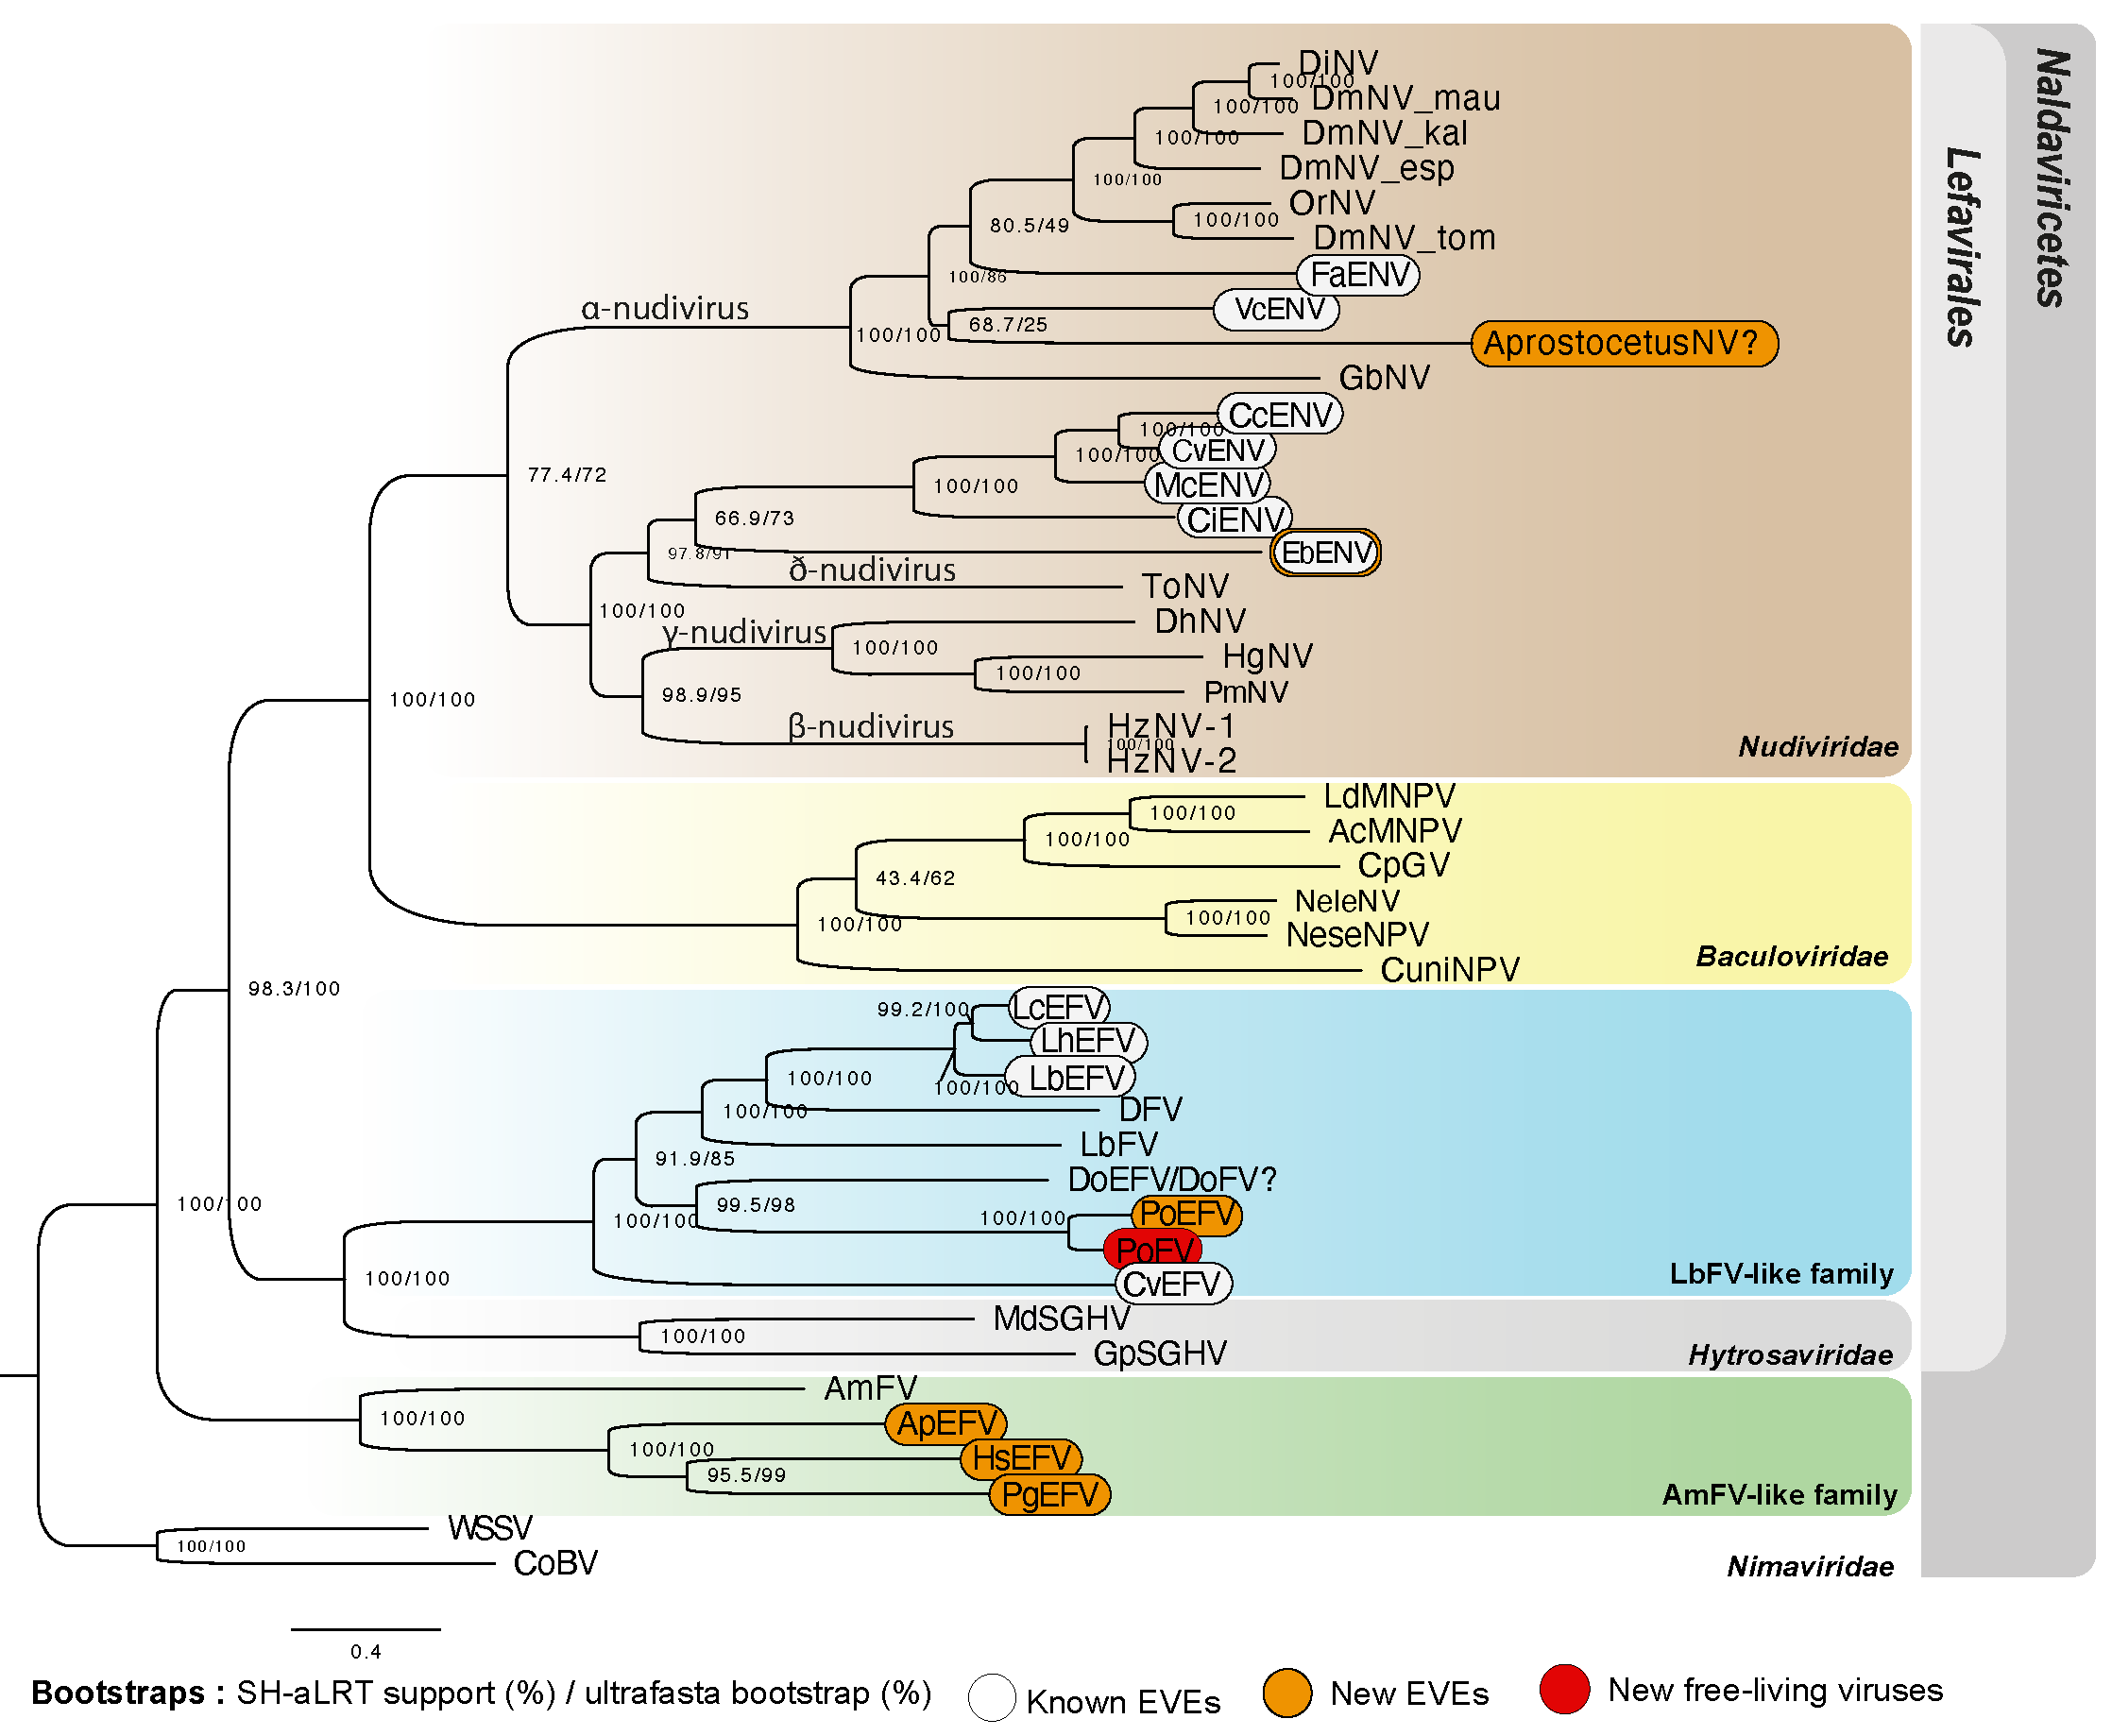
\includegraphics[width=\linewidth,height=\textheight,keepaspectratio]{PhD-master/figures/dsDNA_phylogeny.pdf}
\caption[Paper1:Phylogenetic relationships among endogenized and "free-living" dsDNA viruses]{\textbf{Phylogenetic relationships among endogenized and "free-living" dsDNA viruses}. Specifically, this figure shows the relationships between \textit{Naldaviricetes} double-stranded DNA viruses and EVEs from hymenopteran species, where at least 3 endogenization events were found. This tree was computed using maximum likelihood in Iqtree (v2) from a 38,293 long protein alignment based on the concatenation of 142 viral genes. Confidence scores (aLRT\%/ultra-bootstrap support\%) are shown at each node. The scale bar indicates the average number of amino acid substitutions per site. Previously known EVEs  are in white, those from the present study in orange, and leaves inferred as free-living viruses are in red.  All the best partitioned models can be found on the GitHub file : \href{https://github.com/BenjaminGuinet/PhD_defense/blob/main/Supplementary_paper1/dsDNA_phylogeny_best_ML_partitions.nxs}{dsDNA\_phylogeny\_best\_ML\_partitions.nxs}. All free-living dsDNA viruses used in this phylogeny were obtained from published complete viral genomes. More details on the phylogenetic inference can be found in methods.}
\label{figure:dsDNA_phylogeny}
\end{figure}

We found 5 new cases of endogenization involving multiple EVEs from dsDNA viruses belonging to \textit{Nudiviridae}, LbFV-like and AmFV-like families. 

Two of them involve parasitoid species, i.e. \textit{Platygaster orseoliae} and an \textit{Aprostocetus} species. For \textit{Aprostocetus}, we detected 6 EVEs related to nudiviruses branching between the Chalcidoidea and the Diaprioidea superfamilies (\figurename{\ref{figure:Multiple_EVEs_COV_GC}}). Among these EVEs we found four with an annotation : \textit{lef-4}, \textit{Ac68/pif-6}, GrBNV\_gp19/60/61-like proteins,  and a rep-like protein. In the absence of closely related sequences or RNA seq data, we cannot investigate if these elements have been domesticated. The \textit{P. orseoliae} case involve the recently characterized putative family of filamentous viruses \citep{lepetit_genome_2017}. The free-living LbFV virus is the only representative of this putative family and has been identified as a source of adaptive genes in \textit{Leptopilina} wasps that parasitize \textit{Drosophila} flies, with 13 virally-derived genes involved in the production of VLPs protecting the wasp's eggs from encapsulation (Di Giovanni et al., 2020). In \textit{P. orseoliae}, 15 genes homologous to LbFV were detected (out of 108 ORFs in the LbFV genome; median E-value = 9.39e-21 [min = 2.617e-76, max = 4.225e-08], \figurename{ \ref{figure:Porseoliae_endogenization_events_gene_plot}}-A). Among these 15 genes, 5 were also endogenized in \textit{Leptopilina} species (named LbFV\_ORF58:DNApol, LbFV\_ORF78, LbFV\_ORF60:LCAT, LbFV\_ORF107 and LbFV\_ORF85) (Di Giovanni et al., 2020). Assuming the ancestral donor virus contained the same 108 genes as LbFV, the number of shared genes in these two independent domestication events is higher than expected by chance (one-sided binomial test: x = 5, n = 15, p = 13/108, p= 0.02682), suggesting  that similar functions could have been retained in both lineages (see additional information in \hyperref[sec:SI-2]{supplemental information}). Notably, we also found within the \textit{P. orseoliae} assembly a new "free-living" virus among scaffolds noted as F or X, related to LbFV, that we propose to call PoFV (Platygaster orseoliae filamentous virus) (see fig. \ref{figure:dsDNA_phylogeny} and  \hyperref[sec:SI-2]{supplemental information} for details). This virus is the closest relative to the EVEs found in \textit{P. orseoliae} and is composed of 136 ORFs \figurename{\ref{figure:Porseoliae_endogenization_events_gene_plot}}-B). Using this putative whole genome viral sequence to search for homologous genes in the \textit{P. orseoliae} genome, we were able to detect a total of 139 convincing EVEs (corresponding to 89/136 PoFV ORFs). 44/89 of these EVEs presented signs of domestication using paralogs, with \textit{dN/dS} significantly lower than 1 (see details in  \hyperref[sec:SI-2]{supplemental information}). Although functional studies are clearly needed to confirm that these virus-derived genes are involved in the production of VLPs as in \textit{Leptopilina} (Di Giovanni et al., 2020), we see Platygaster orseoliae endogenous viral elements (PoEFVs) as good candidates for viral domestication, which could possibly be involved in counteracting the immune system of its dipteran host (from the Cecidomyiidae family \citep{buhl_new_2016}). To our knowledge, this is the first report of a massive viral endogenization and putative domestication within the \textitit{Platygastroidea} superfamily.

The other three cases involved ant species : \textit{Harpegnathos saltator} (EsEFV) 
(12EVEs and 6dEVEs), \textit{Pseudomyrmex gracilis} (PgEFV) (9EVEs and 1dEVE), \textit{Aphaenogaster picea} (ApEFV) (7EVEs). These endogenized elements are related to a poorly characterized family of filamentous viruses denoted AmFV \citep{hartmann_dynamics_2015,yang_genomics_2022}. In \textit{H. saltator}, 9 genes deriving from an AmFV-like virus were detected (including 3 genes that have been previously identified by \citep{flynn_assessing_2019}). Intriguingly, all these genes presented  numerous paralogs within the genomes (135 in total) (\figurename{\ref{figure:Multiple_new_endogenization_events_gene_plot}} and \figurename{\ref{figure:Multiple_EVEs_COV_GC}}), with 22 copies for AmFV\_0062 (\textit{pif-1}), 18 for AmFV\_0102 (\textit{pif-2}), 51 for AmFV\_0090 (\textit{pif-3}), 24 for AmFV\_0044 (\textit{integrase}), 13 for AmFV\_0079 (\textit{p74}), 5 for AmFV\_0047 (\textit{RNA polymerase}), 19 for AmFV\_0126 (Unknown), 23 for AmFV\_0168 (Unknown) and  7 for AmFV\_0154 (Unknown). Most paralogs were found in scaffolds exceeding the expected size for any virus sequence (min = 23,726bp, mean = 326,262bp, max = 2,693,376bp). In addition, all scaffolds do include transposable elements and eukaryotic genes making them undoubtedly endogenized. Accordingly, our pipeline attributed the highest confidence index A for 104 of them (out of 135). The \textit{P.gracilis} genome revealed 9 EVEs, including homologs of \textit{pif-1}, \textit{pif-3}, \textit{RNA polymerase}, \textit{ac81}, \textit{integrase} and \textit{odv-e56} (\figurename{\ref{figure:Multiple_new_endogenization_events_gene_plot}}). Notably, one of the 9 EVEs (AmFV\_059, of unknown function) shows both a \textit{dN/dS} $<$ 1 (mean= 0.1747, p-value 5.877e-02), and a very high TPM value (362836 TPM from whole body tissues). Finally, in \textit{A. picea}, 7 EVEs were detected, including homologs of \textit{pif-1}, \textit{pif-3}, \textit{integrase}, \textit{odv-e56} and \textit{p74} (\figurename{ \ref{figure:Multiple_new_endogenization_events_gene_plot}}). No raw reads data were available for this species, precluding coverage-based inferences. Since there were neither orthologs or paralogs for these genes to compute \textit{dN/dS} analyses, nor transcriptomic data, it was not possible to infer their domestication status. At this stage it is thus not possible to conclude as to the functions of these genes in \textit{H. saltator}, \textit{P. gracilis} and \textit{A. picea}, but this surely deserves further attention.

 
\section{Discussion}

All kinds of viruses can integrate arthropod genomes, although the mechanisms underlying these phenomena remain unclear \citep{katzourakis_endogenous_2010, gilbert_diversity_2022}. Prior to the present analysis, 28 viral families had been described as involved in endogenization in arthropods \citep{gilbert_diversity_2022}. Our study of Hymenopteran genomes further revealed the ubiquity of this phenomenon, with at least 40 viral families (or family-like clades) involved. Of the 1,261 EVEs found, the average identity with the closest known viral proteins was 36.32\% [min = 15.7\%, max = 99.1\%]. Although this large overall divergence suggests ancient events, it does not exclude the possibility that some of the integrations are recent, because free-living viral relatives of the true donors may be unknown or extinct \citep{junglen_virus_2013}.

In the following section, we will first discuss why double-stranded DNA viruses, in comparisons with other viral genomic structures (ssDNA, dsRNA, ssRNA), are more often endogenized than expected. We will then discuss hypotheses that could explain why we found a higher rate of endogenization of dsDNA viruses among  endoparasitoids compared to ectoparasitoids or free-living hymenopterans, which also translates into more frequent events of domestications.\\

\textbf{\\dsDNA viruses are more frequently involved in endogenization than expected by chance}
\\Despite the observations that all viral genomic structures can be involved in endogenization, we clearly identified differences in their propensity to do so. Based on a comparison between the respective proportions of the various viral categories in the inferred endogenization events and in public databases, we found that dsDNA viruses are much more represented than expected, while ssRNA viruses are under-represented (\figurename{ \ref{figure:Genomic_structure_and_families_Events_distributions}-A}). We acknowledge that current knowledge on the actual diversity of free-living viruses (as approximated through the NCBI taxonomy database) remains incomplete, but the strength of the effect reported here makes this conclusion rather robust to variations in the null distribution. On the basis of current knowledge, RNA viruses, and in particular ssRNA viruses, appear to be much more diversified and prevalent than DNA viruses in insects. We note that viral-metagenomic studies often focus either on DNA or RNA viruses, and as such do not provide an accurate and unbiased picture of the extent viral diversity. To gain insights on this topic, we may thus focus on model systems where long-lasting research efforts have likely produced a more reliable picture. The Honeybee \textit{Apis mellifera} is probably the most studied of all Hymenopteran species. In honeybees, the great majority of known viruses belongs to the RNA world \citep{chen_honey_2007}, with very few exceptions \citep{yang_genomics_2022}. Similarly, until 2015, only RNA viruses were known to infect the fruit fly \textit{Drosophila melanogaster}, despite the extensive research conducted on this model system \citep{webster_discovery_2015}. A very limited set of DNA viruses has now been described from this species \citep{wallace_discovery_2021} but clearly, RNA viruses dominate the \textit{Drosophila} viral community, both in terms of diversity and prevalence. In support of this view, recent studies revealed the very elevated absolute diversity of RNA viruses. For instance, a survey of 600 insect transcriptomes recovered more than 1,213 RNA viruses belonging to 40 different families \citep{wu_abundant_2020-1}. Although, obviously, this study does not inform on the diversity of DNA viruses, it shows that the RNA virome of insects is both prevalent (e.g., in this study, 15\% of all insects were infected by a single Mononegales-like virus) and extremely diversified \citep{wu_abundant_2020-1}. Actually, this view appears to hold at the larger scale of eukaryotes \citep{koonin_origins_2015}. Taking into account this patent abundance of ssRNA viruses in insects, our study indicates they are by far less frequently endogenized than their dsDNA counterparts in hymenopterans. Notably, a similar trend was recently reported in a study including a diverse set of eukaryotes \citep{irwin_systematic_2022}.

Most of the major endogenization events characterized so far in hymenopterans involve dsDNA viruses from the \textit{Nudiviridae} family \citep{cheng_nudivirus_2020, burke_common_2019,pichon_recurrent_2015,bezier_polydnaviruses_2009-1, cheng_brown_2014, zhang_chalcid_2020, gilbert_diversity_2022}. Our study further confirms that this viral family represents a major source of exogenous and sometimes adaptive genes for Hymenoptera. Indeed, 28 new independent endogenization events involve this family, among which 9 are shared by at least two related species (\figurename{ \ref{figure:Genomic_structure_and_families_Events_distributions}-B}, \figurename{\ref{figure:Event_phylogeny}}). 
The major contribution of nudiviruses to endogenization may be explained by their wide host range in arthropods \citep{wang_nudivirus_2007}.  Their nuclear replication constitutes another plausible explanatory factor \citep{velamoor_visualizing_2020}, since it may facilitate contact with host DNA. In addition, their tropism for gonads may favor the endogenization in germinal cells \citep{burand_sexually_2009}. In fact, nuclear replication is a feature shared by nearly all families of dsDNA viruses found in our analysis : \textit{Baculoviridae}, \textit{Iridoviridae}, \textit{Phycodnaviridae}, \textit{Nimaviridae} \textit{Caulimoviridae}, \textit{Herpesviridae}, \textit{Asfaviridae} (at early times) \citep{schmid_dna_2014, harrison_ictv_2020, international_committee_on_taxonomy_of_viruses_virus_2012, teycheney_ictv_2020,verbruggen_molecular_2016}, Apis-filamentous-like \citep{clark_filamentous_1978} and LbFV-like families \citep{varaldi_artifical_2006} (the \textit{Poxviridae} viruses, that replicate in the cytoplasm, are thus the only exception). In contrast, most RNA viruses replicate in the cytoplasm. Nuclear replication may thus constitute a general explanation for the elevated propensity of DNA viruses to endogenization. Additionally, we may expect that a DNA molecule, rather than an RNA molecule, is more likely to integrate the insect genome, because the latter requires reverse transcription before possible endogenization.

The \textit{Poxviridae} case indicates that cytoplasmic replication does not necessarily impede endogenization. These viruses do not require nuclear localization to propagate \citep{moss_poxvirus_2013,schmid_dna_2014} and were nevertheless found to be involved in many endogenization events (n=28). A similar pattern was observed in a recent study focusing on ant genomes \citep{flynn_assessing_2019}). Within Poxviridae, entomopoxviruses were particularly involved in endogenization events (n=18) with four cases of EVEs shared between several closely related species (\figurename{ \ref{figure:Genomic_structure_and_families_Events_distributions}-B}).\\

\textbf{\\Factors behind variations in endogenization and domestication rates }
\\Several recent studies have uncovered abundant EVEs in insect genomes \citep{flynn_assessing_2019, ter_horst_endogenous_2019, russo_novel_2019}, with huge variation in abundance between species.  For instance, in their analysis based on 48 arthropod genomes, \citep{ter_horst_endogenous_2019} found that the number of EVEs ranged between 0 and 502. Although insect genome size and assembly quality may partly explain this variation \citep{gilbert_diversity_2022}, the underlying biological factors are generally unknown. In this study, we tested the hypothesis that the insect lifestyle may influence both the endogenization and domestication rates. We used a Bayesian approach to reconstruct ancestral states throughout the phylogeny of Hymenoptera, thus accounting for uncertainty, and found that endoparasitoidism, in comparison with other lifestyles, tends to promote dsDNA viral endogenization. Notably, this conclusion was not the artefactual consequence of differences in genome assembly quality. In fact, the quality of genome assemblies was correlated with the lifestyle in our data set, but the genomes of endoparasitoid species were generally less well assembled than those of free-living species. If anything, this difference should reduce the power for detecting endogenization events in endoparasitoids, where our analysis detected an excess of such events. Our estimate of the effect sizes (with 2.47 times more endogenization events in endoparasitoids than in  free-living species) should thus be seen as conservative. 
Why do endoparasitoid wasps tend to undergo more endogenization than others? We initially had in mind two non-exclusive hypotheses that remain plausible explanations for the observed pattern. First, endoparasitoids may be more intensively exposed to viruses. In addition, or alternatively, endoparasitoids may have a higher propensity to endogenize and retain viral genes. 

Several factors come in support of the first hypothesis. Endoparasitoid larvae grow by definition inside their host's body, and such a close interaction implies that any endoparasitoid individual will also be interacting with its host's viruses. Accordingly, the best studied cases of viral domestication in wasps involve nudiviruses, that are known to replicate in their caterpillar hosts \citep{burke_rapid_2018,pichon_recurrent_2015,bezier_polydnaviruses_2009-1}. Another putatively important factor is the presence of virus in the venoms that parasitoids inject into hosts together with their eggs. These are known to protect the offspring against the host's immune response, and to manipulate the host physiology \citep{asgari_venom_2011} but this feature could favor the subsequent spread of viruses in wasp populations: by colonizing the venom-producing tissues (venom gland or calyx, depending on the species biology) viruses may secure an effective pseudo-vertical transmission and  thus maintain themselves efficiently in wasp populations. Numerous endoparasitoid viruses benefit from such pseudo-vertical transmission  \citep{varaldi_artifical_2006,renault_cypovirus_2003}, including some whose relatives have been endogenized and domesticated by endoparasitoids (Di Giovanni et al., 2020). The presence of viruses within venoms may also facilitate horizontal transmission between conspecifics in the case of superparasitism, as observed in the \textit{Drosophila} parasitoid \textit{Leptopilina boulardi} \citep{varaldi_infectious_2003}. Although this effect may also be at play for some ecto-parasitoid species \citep{zhang_novel_2021}, we expect it to be more pronounced for endo-parasitoid species since they have a closer interaction from the inside of their hosts. 
Generally, endoparasitoids may thus carry a higher load of non-integrated viruses than other hymenopterans. However, if this effect is at play, we expect to have an "endoparasitoid" effect for all viruses, whatever their genomic structure. For instance, we would expect such an effect to be detected for ssRNA viruses, which are involved in the greatest number of endogenization events (\figurename{\ref{figure:Genomic_structure_and_families_Events_distributions}}-A).  This was not the case, since only dsDNA viruses were more frequently endogenized in endoparasitoids. Thus, we argue that this hypothesis is unlikely to explain the observed pattern.

The second hypothesis posits that endoparasitoids are more frequently selected for retaining  virally-derived genes than ectoparasitoid or free-living hymenopterans. In our analysis, domestication events are most frequently observed in endoparasitoids (over 3 times more frequently than in other hymenopterans). Obviously, this may be at least partly explained by the higher input discussed above (the higher endogenization rate). Yet, once this effect is controlled for, a trend towards a higher rate of domestication remains. More specifically, the likelihood of domestication following endogenization was significantly higher in endoparasitoids than in ectoparasitoids, but was not significantly higher than in free-living species. This latter lack of significant difference may be biologically explained if a single domestication event precludes the domestication of additional EVEs, while not affecting the rate of non-adaptive endogenization. This would "dilute" the signal along branches involved in domestication. If this effect is at play, then it reduces considerably the power of our analysis to detect any difference on the rate of domestication between lifestyles. Indeed, in all known cases, only one domesticated virus has been documented, suggesting that further domestications are not beneficial once a viral machinery has been recruited by a wasp lineage.

Whether or not the rate of domestication \textit{per se} is higher in endoparasitoids than in other hymenopterans, the selective advantages brought by these viral genes in endoparasitoids should be discussed. It has been demonstrated in a few model systems that EVEs may confer antiviral immunity against related "free-living" viruses via the piRNA pathway  \citep{suzuki_non-retroviral_2020,whitfield_diversity_2017}. Yet, to our knowledge, such an effect has only been demonstrated against RNA viruses, so that it would not explain the excess of DNA viruses documented here. Furthermore, the sequence identities with known viral sequences, which is needed for this mechanism to work, is low in our dataset. Accordingly, previous work revealed that EVE-derived piRNAs studied in 48 arthropod species were also probably too divergent to induce an efficient antiviral response \citep{ter_horst_endogenous_2019}. At that stage, the ability of EVEs to generate PIWI-interacting RNAs that play a functional role in antiviral immunity seems questionable. Further studies involving small RNA sequencing in hymenopterans would be required to shed light on this issue.
Protection of the eggs and larvae against the host immune system is recognized as an important trait, where EVEs play a critical role. Because of their peculiar lifestyle, endoparasitoids are all targeted by the host immune system, a matter of life or death to which other hymenopterans are not exposed to. Several cases of endogenization and domestication in endoparasitoids, all involving dsDNA viruses, are thought to be related to this particular selective pressure \citep{bezier_polydnaviruses_2009-1,volkoff_analysis_2010,pichon_recurrent_2015,burke_common_2019,di_giovanni_behavior-manipulating_2020}). The parasitoids appear to have co-opted the viral fusogenic property to address their own proteins (VLPs) or DNA fragments (polydnaviruses) to host immune cells, thereby canceling the host cellular immune response. The above-hypothesized high exposure of endoparasitoids to viruses, together with this unique selective pressure, may act in concert to produce the pattern documented here: a strong input, that is, a diverse set of putative genetic novelties, combined with a strong selective pressure for retaining some of them. The observed excess of dsDNA viruses  may be an indication  that these viruses display a better potential for providing adaptive material in this context. In the cases of polydnaviruses (found in some Braconidae and some Campopleginae), it appears that one way to efficiently deliver virulence factors to the host cell is by addressing DNA circles that ultimately integrate into the host immune cells and get expressed \citep{chevignon_functional_2014, chevignon_cotesia_2018}. The DNA which is packed into the mature particles typically encodes virulence proteins deriving from the wasp \citep{espagne_genome_2004}. This means that, at least for these cases, the viral system should be able to pack DNA, which is most likely a feature that DNA viruses may provide. Such an argument does not hold in the VLP systems, where only proteins are packed in viral particles, and it is unclear why EVEs deriving from dsDNA viruses would be more able to fulfill such a function. Here other features of dsDNA viruses come into mind as possibly important factors: their large genome size, and their large capsids and envelopes \citep{chaudhari_scaling_2021}. These may predispose dsDNA viruses to be domesticated, since abundant quantities of venoms have to be transmitted in order to efficiently suppress the host immune response.


\section{Conclusion}

Our analysis has revealed a large set of new virally-derived genes in Hymenoptera genomes. Those genes were deriving from viruses with any genomic structures, although dsDNA viruses were disproportionately involved in endogenization and domestication. 
Importantly, our analysis revealed that endogenization rate and the absolute number of domestication events involving dsDNA viruses was increased for endoparasitoids compared to other lifestyles. 
Among the new cases of endogenization and domestication, we uncovered new events revealing common features with previously known cases of viral domestication by endoparasitoids, such as in the Platygastroidea \textit{Platygaster orseoliae}. This is to our knowledge the first case reported in the superfamily Platygastroideae, thus extending the diversity of Hymenoptera concerned by viral domestication. We propose that the higher rate of endogenization and higher number of domestication events in endoparasitoids is a consequence of the extreme selective pressure exerted by the host immune system on endoparasitoids. This extreme selective pressure may select endoparasitoids for retaining a viral machinery that could help them address virulence factors to their hosts. We expect this process to be widespread among insect species sharing the same lifestyle.

\section{Material and methods}


\subsection{Genome sampling, assembly correction and assembly quality}
\label{sec:MM-1}

A bioinformatic pipeline mixing sequence homology search, phylogeny, genomic environment, and selective pressure analysis was built to search for viral endogenization and domestication events in Hymenoptera genomes. We used 133 genome assemblies in total, of which 101 were available on public repositories (NCBI and BIPPA databases) and 32 were produced by our laboratory (all SRA reads and assemblies available under the NCBI submission ID : SUB11373855). Concerning the last 32 samples, DNA was extracted on single individuals (usually one female) or a mix of individuals when the specimens were too small using Macherey-Nagel extraction kit, the DNA was then used to construct a true seq nano Illumina library at Genotoul platform (Toulouse, France). The sequences were generated from HiSeq 2500 or HiSeq 3000 machines (15Gb/sample). The paired-end reads were then quality trimmed using fastqmcf (-q15 --qual-mean 30 -D150, \href{https://GitHub.com/ExpressionAnalysis/ea-utils}{GitHub}) and assembled using IDBA-UD \citep{peng_idba-ud_2012}. All sample information can be found on the GitHub file: \href{https://github.com/BenjaminGuinet/PhD_defense/blob/main/Supplementary_paper1/All_sample_informations.txt}{All\_sample\_informations.txt} and is available under the NCBI Biosample number : SUB11338872.

The size of the 133 assemblies ranged from 106.14mb to 2102.30mb. We kept only genome assemblies containing at least 70\% non-missing BUSCO genes (124/133 genomes, \citep{simao_busco_2015}) (all genome information can be found on the GitHub file : \href{https://github.com/BenjaminGuinet/PhD_defense/blob/main/Supplementary_paper1/Assembly_genome_informations.csv}{Assembly\_genome\_informations.txt})). In addition, when the raw reads were available, we used the MEC pipeline \citep{wu_mec_2020} to correct possible assembly errors. Although some genomes were highly fragmented (such as the 32 genomes we generated since they were obtained using short reads only), the N50 values (min: 3542bp) were equal to or larger than the expected sizes of genes known to be endogenized and domesticated (min known domesticated EVE : 165bp) indicating that most of the putative EVEs should be detected entirely.

Out of the 32 samples sequenced by our laboratory for this study, one (corresponding to \textit{Platygaster orseoliae}) gave unexpected results. After assembly and BUSCO analysis, two sets of contigs were identified:  one with only 4X coverage on average, and one with 33X on average. The phylogeny of these different BUSCOs gene sets showed that the low-coverage scaffolds likely belong to an early diverging lineage of Chalcidoidea  (\figurename{\ref{figure:Event_phylogeny}}), whereas the 33x scaffolds belong to the target species \textit{P. orseoliae}. This result suggests that the pool of 10 individuals used for sequencing was likely a mix of two species. A phylogenetic study based on Ultra Conserved Elements (UCEs) obtained from several species of Chalcidoidea \citep{rasplus_first_2020, cruaud_optimized_2019} allowed to identify the unknown species as sister to  \textit{Aprostocetus sp}  (Eulophidae) (see details in the \hyperref[sec:SI-2]{supporting information} and \figurename{\ref{figure:UCEs}}). In the figures and tables, the name putative\_ \textit{Aprostocetus}\_sp was consequently assigned to the unknown sample. However, since the lifestyle and identity of this species are uncertain, we did not include the corresponding scaffolds in the main analysis. The scaffolds belonging to this putative\_\textit{Aprostocetus}\_sp. (i.e : all scaffolds with a mean coverage $<$ 10X) were removed from the \textit{P. orseoliae} assembly file hosted in NCBI.  

\subsection{Pipeline outline}
\label{sec:MM-2}\\
EVEs were identified from the 124 Hymenoptera assemblies using a sequence-homology approach against a comprehensive viral protein database (including all categories of viruses : ssDNA, dsDNA, dsRNA and ssRNA). In order to validate viral endogenization within Hymenoptera genomes, we developed an "endogenization confidence index" ranging from A to X (\figurename{\ref{figure:Bioinformatic_pipeline}}-7). This index takes into consideration the presence of eukaryotic genes and/or transposable elements around candidate loci, and scaffolds coverage information (coverage for a valid candidate should be similar to that found in BUSCO containing scaffolds). Finally, the pipeline also included an assessment of the evolutionary history and of the selective regime shaping the candidates (based on \textit{dN/dS} and/or expression data).

\subsection{Hymenoptera phylogeny}
\label{sec:MM-3}

The phylogenetic reconstruction of the 124 Hymenoptera species was performed based on a concatenation of the 375 BUSCO proteins. The analysis was conducted by maximum likelihood via Iqtree2 \citep{minh_iq-tree_2020} selecting the best model \citep{kalyaanamoorthy_modelfinder_2017}. The tree was rooted via two species of the Coleoptera order (\textit{Anoplophora glabripennis} and \textit{Tribolium castaneum}). Bootstrap scores were evaluated using the UFboot approach \citep{hoang_ufboot2_2018}. The results found were consistent with a previous, more comprehensive study \citep{peters_evolutionary_2017}. 

subsection{Search for viral homology}
\label{sec:MM-4}

We collected all protein sequences available in NCBI virus database \citep{hatcher_virus_2017}, removing phage and polydnavirus (virulence genes from wasp origin found within PDVs) sequences. This database contained 849,970 viral protein sequences (download date : 10/10/2019), to which the 40 putative viral proteins encoded by the \textit{Hyposoter didymator} genome were added (so-called IVSPER sequences, \citep{volkoff_analysis_2010-1}). The sequence homology search was performed with a BlastX equivalent implemented in Mmseqs2 \citep{steinegger_mmseqs2_2017}) using each genome assembly as queries and the viral proteins collected as database. The result gave a total of 81,953,678 viral hits (max E-value 5e-04 with an average of 660,916 hits per genomes). We kept only candidates with a percentage coverage of the viral protein $>$= 30\%, an identity score $>$= 20\% and an E-value score $<$ 5e-04 (\figurename{ \ref{figure:Bioinformatic_pipeline}}-1). The threshold parameters were optimized to maximize the detection of the 13 endogenous viral sequences within the genus \textit{Leptopilina} (Di Giovanni et al., 2020). Once all the viral hits were recovered, we formed putative EVEs loci (n=238,108) corresponding to the overlap of several viral hits on the same scaffold using the GenomicRanges R package \citep{lawrence_software_2013} (\figurename{ \ref{figure:Bioinformatic_pipeline}}-2).
To remove false positives corresponding to eukaryotic genes rather than viral genes, we then performed another generalist sequence homology search against the Nr database (downloaded the 09/11/20) using mmseqs2 search (-s 7.5, E-value max = 0.0001) (\figurename{ \ref{figure:Bioinformatic_pipeline}}-3). We did not select our candidate based on the best hit, since it does not necessarily reflect the true phylogenetic proximity. Instead, candidates with more than 25 hits with either eukaryotic non-hymenoptera species or prokaryotic species were removed, except if they also had hits with at least 10 different virus species (bits $>$= 50). We chose to eliminate Hymenoptera hits from the database because if a real endogenization event concerns both one of the 124 species of our dataset and some species in the NCBI database, then an apparent "Hymenoptera" hit will be detected, possibly leading to its (unfair) elimination.
Since viral diversity is  poorly known, we also kept sequences with even one single viral hit, as long as it did not have more than 5 eukaryotic  or prokaryotic hits. Using these filtering criteria we removed a total of 234,036/238,108 (98,3\%) candidate loci leaving 4,072 candidates with convincing homology to viral proteins. Note that among these loci a certain proportion actually corresponded to non-endogenized "free-living" viruses. To study the evolutionary history of these candidate EVEs, we then performed a general protein clustering of all the candidates and the NCBI viral proteins (\figurename{ \ref{figure:Bioinformatic_pipeline}}-4, Mmseqs cluster; thresholds : E-value 0.0001, cov\% 30, options : --cluster-mode 1 --cov-mode 0 --cluster-reassign --single-step-clustering \citep{steinegger_clustering_2018}.

We eliminated from the dataset the chuviral glycoproteins that have been captured by LTR retrotransposons \citep{dezordi_and_2020}, as these loci have complex histories mostly linked to the transposition activity after endogenization. For this purpose, we systematically searched among the candidates for the presence of TEs within or overlapping with the EVE (see the GitHub file : \href{https://github.com/BenjaminGuinet/PhD_defense/blob/main/Supplementary_paper1/All_TEs_overlapping_with_EVEs.txt}{All\_TEs\_overlapping\_with\_EVEs.txt}). Only one cluster (Cluster4185) was concerned by such a situation (chuviral glycoproteins overlapping to Gypsy/LTRs). It was detected in 89/124 species (1074 total copies, median = 7 copies/species, max = 244, min =1), and was probably similar as the one described in \citep{li_unprecedented_2015}. 

\subsection{Evolutionary history and selection pressure acting on endogenous loci}

\subsection{Arguments for endogenization} 
\label{sec:MM-5}

Among all the candidates for endogenization there were probably false positives that corresponded either to natural contaminants (infecting viruses sequenced at the same time as the eukaryotic genome) or laboratory contaminants (virus accidentally added to the samples). One way to filter these cases was to study (i) the genomic environment (are there other eukaryotic genes or transposable element on the same scaffolds?) and (ii) metrics such as G+C\% (used only for read coverage/GC plots) and scaffold coverage depth around candidate loci (are they the same as scaffolds containing housekeeping genes?). All of these data were used to establish confidence in the endogenization hypothesis, scaled from A to X (\figurename{ \ref{figure:Bioinformatic_pipeline}}-7).

\textbf{(i) Scaffolds sequencing depth (\figurename{ \ref{figure:Bioinformatic_pipeline}}-5) :}
In order to support the hypothesis that a scaffold containing candidate EVEs was part of the Hymenoptera genome, we studied the sequencing depth of the scaffolds. If the sequencing depth of a candidate scaffold was not different from the depth observed in scaffolds containing BUSCO genes, then this scaffold was likely endogenized into the Hymenoptera genome. Hence, when DNA reads were available (\figurename{\ref{figure:Genomes_qualities_and_origins}}), we measured this metric by mapping the reads on the assemblies using hisat2 v 2.2.0 \citep{kim_graph-based_2019}. An empirical p-value was then calculated for each scaffold containing a candidate EVE. To calculate this empirical p-value, we sampled 500 loci of the size of the scaffold of interest within BUSCO scaffolds. These 500 samples represented a null distribution for a scaffold belonging to the Hymenoptera genome. The p-value then corresponded to the proportion of BUSCO depth values that were more extreme than the one observed in the candidate scaffold (two-sided test). We used a threshold of 5\% and a 5\% FDR (multipy python package \citep{puolivali_influence_2020}). 

\textbf{(i) Genomic environment and scaffold size} (\figurename{ \ref{figure:Bioinformatic_pipeline}}-6)
Another way to rule out contaminating scaffolds was to look for the presence of eukaryotic genes and transposable elements in the scaffolds containing candidate EVEs, assuming that their presence in a viral scaffold is unlikely. Indeed, so far, very few viral genomes have been shown to contain transportable elements \citep{miller_virus_1982,gilbert_population_2014,gilbert_continuous_2016,gilbert_viruses_2017,loiseau_wide_2020} because TE insertions are mostly deleterious and are therefore quickly  eliminated by negative selection \citep{gilbert_continuous_2016, gilbert_viruses_2017}. We searched for transposable elements by a BlastX-like approach (implemented in Mmseqs2 search -s 7.5), taking as query the scaffolds of interest and as database the protein sequences of the transposable element (TE) available in RepeatModeler database (RepeatPeps, v2.0.2) \citep{flynn_repeatmodeler2_2020}. We only kept hits with an E-value $<$ 1e-10 and with a query alignment greater than 100aa. We then merged all overlapping hits and 
counted the number of TEs for each scaffold. To find eukaryotic genes within genomes we used Augustus 3.3.3 \citep{stanke_augustus_2004} with BUSCO training and then assigned a taxonomy to these genes via sequence homology with Uniprot/Swissprot database using mmseqs2 search \citep{steinegger_mmseqs2_2017}, and only retained genes assigned to insects.

Accordingly, the scaffolds were scored as follows (\figurename{ \ref{figure:Bioinformatic_pipeline}}-7) : 
\begin{itemize}
    \item A: scaffolds with a corrected coverage p-value $>$ 0.05 and at least one eukaryotic gene and/or one repeat element, 
    \item B: scaffolds with at least one eukaryotic gene and/or one repeat element but no coverage data available, 
    \item C: scaffolds with a corrected coverage p-value $>$ 0.05 and neither eukaryotic gene nor transposable element, 
    \item D: scaffolds with a corrected coverage p-value $<$ 0. 05 and whose coverage value was higher than the average of the scaffolds containing BUSCOs (as it is difficult to imagine that an endogenized scaffold present a lower coverage than expected, whereas a higher coverage could correspond to the presence of repeated elements that inflate the coverage of the scaffold for example) but with at least 5 eukaryotic genes and/or a repeated element (in total), 
    \item E: scaffolds presenting no DNA seq coverage data available and no eukaryotic gene nor transposable element detected, 
    \item F: scaffolds presenting a corrected p-value of coverage $<$ 0.05 and less than 5 eukaryotic genes without any transposable elements; this category may rather correspond to free-living viruses.
    \item X: scaffolds with a corrected p-value < 0.05 and neither eukaryotic gene nor transposable element; This category may rather correspond to free-living viruses.
\end{itemize}


\subsection{Inference of endogenization events}
\label{sec:MM-6}

Because several EVEs may derive from the same endogenization event, we sought to aggregate EVEs into unique events. We aggregated into a single event, firstly (i) all the EVEs present on the same scaffolds, and secondly (ii) all the EVEs that presented the same taxonomic assignment at the level of the viral family.  These two steps were sufficient to aggregate EVEs in the simplest case of events involving only one species (but possibly several EVEs).  

To further characterize the endogenization events including more than one Hymenoptera species, we also relied on phylogenetic inference.  To this end, the protein sequences belonging to each of the clusters (containing both viral proteins and candidate EVEs) were first aligned with clustalo v1.2.4 \citep{sievers_fast_2011} in order to merge possible candidate loci (which may in fact correspond to various HSPs). All loci (=HSPs) within the same scaffold presenting no overlap in the alignment were thus merged, as they probably correspond to multiple HSPs and not duplications.  We then performed a new codon alignment from the augmented sequences in the clusters using the MACSE v2 alignsequence program \citep{ranwez_macse_2018} (\figurename{ \ref{figure:Bioinformatic_pipeline}}-8). This alignment allowed us to obtain a protein and nucleotide codon alignment. We used the protein alignment to infer the phylogeny of each cluster with the program Iqtree2 v2.1.2 \citep{minh_iq-tree_2020} (-m MFP -alrt 1000 (partitioned))(\figurename{ \ref{figure:Bioinformatic_pipeline}}-9).
No trimming was performed at the amino-acid level, since this may result in loss of topology information \citep{tan_current_2015,ranwez_chapter_2020}. However, since it can affect branch length, only codon alignment was trimmed at the protein level via Trimal v1.2 (\figurename{ \ref{figure:Bioinformatic_pipeline}}-10) (-backtrans -automated1) \citep{capella-gutierrez_trimal_2009}. 
We then exploited the information from the cluster phylogenies to form the endogenization events. EVEs potentially deriving from the same event should be supported by the formation of the same well-supported monophyletic clade (bootstrap $>$ 80) both in the gene tree and the Hymenoptera tree (allowing gene losses in 20\% of the species concerned by the monophyletic group). EVEs were possibly aggregated within the same event only if the Hymenoptera belonged to the same family.  (\figurename{ \ref{figure:Bioinformatic_pipeline}}-11). Finally, the clustering of multiple EVEs within the same scaffold in one species was used to aggregate the homologous EVEs found in a related species within the same shared event, even if they were on different scaffolds (\figurename{ \ref{figure:Bioinformatic_pipeline}}). For details, see some canonical examples in \figurename{ \ref{figure:Event_assignation_examples}}. 

For events shared by several species, we were also able to analyze gene synteny around putative EVEs. To do this, we conducted the equivalent of an all vs all TblastX (Mmseqs2 search --search-type 4, max E-value =1e-07) between all the candidate loci within a putative event (deduced from the phylogenetic inference), and then looked for hits (HSPs) between homologous EVEs around the insertions. Because it is possible to find homology between two genomic regions that does not correspond to orthology, for example because of the presence of conserved domains, we had to define a threshold to identify with confidence the orthology signal. We therefore conducted simulations to define this value, based on the well assembled genome of \textit{Cotesia congregata} (GCA\_905319865.3) by simply performing the same all vs all blast analysis against itself (as if the two species considered had the same genome). Based on this, we defined two types of simulated EVEs, (i) independently endogenized EVEs in the genomes of the two "species". This is simply simulated by randomly selecting two different regions in the genomes, and (ii) a shared  simulated EVE that was acquired by their common "ancestor". This is simulated by selecting  the same random genomic location in both "genomes". We then counted the total length of the HSPs found around the simulated insertions all along the corresponding scaffold (i and ii). As the result will obviously depend on scaffold length, we performed these simulations on several scaffold lengths (100000000bp, 10000000bp, 1000000bp, 100000bp and 10000bp). 
We conducted 500 simulations in each scenario, and we measured the cumulative length of homologous sequences by counting the sum of HSPs (bit score $>$ 50). We then defined a threshold for each windows size in order to minimize for the false-positive (FP) and maximize true-positifs (TP)  (thresholds 100000000bp = 172737bp (FP = 0.012, TP= 0.922); 10000000bp = 74262 bp (FP= 0.012, TP=0.878) ; 1000000bp = 21000 bp (FP=0.014, TP=0.28); 100000bp = 1332 bp (FP= 0.012 TP= 0.198) and  10000bp = 180 bp (FP= 0.008, TP= 0.208)). 

Events were linked to viral families based on the closest match information between the viral blastx (GenBank accession number and/or viral protein and/or viral species) and the classification proposed in \citep{shi_redefining_2016}. 


\subsection{Arguments for domestication}}
\label{sec:MM-7}

One way to test for the domestication of an EVEs (dEVEs) was to estimate the ratio (omega) of the number of nonsynonymous substitutions per non-synonymous site (\textit{dN}), to the number of synonymous substitutions per synonymous site (\textit{dS}). If EVEs are evolving neutrally, then the ratio is expected to be equal to 1, whereas if the EVE is under purifying selection, \textit{dN/dS} is expected to be lower than 1. We conducted this analysis on trimmed codon alignments from (\figurename{ \ref{figure:Bioinformatic_pipeline}}-11) via the codeml algorithm from PAML \citep{yang_paml_2007} used through the ETE3 package \citep{huerta-cepas_ete_2016}  (model Muse and Gaut  \citep{muse_likelihood_1994}). We then used a branch model to test the deviation from the null model in which marked branches (called foreground) wich corresponded to the monophyletic EVE clade evolved under a neutral scenario ($\chi^2$ test). The \textit{dN/dS} estimated for the whole clade is then the average of each branch of the clade. The p-values were then adjusted by selecting an FDR of 0.05 \citep{puolivali_influence_2020}, and we estimated the standard errors of \textit{dN/dS} that maximized the likelihood (option getSE = 1). \textit{dN/dS} with dS greater than 10 were removed, since this indicates substitution saturation (\figurename{ \ref{figure:Bioinformatic_pipeline}}-12). 

The other way we choose to study the domesticated nature of a viral gene was to study their expression profile (\figurename{ \ref{figure:Bioinformatic_pipeline}}-13). We reasoned that domesticated genes are likely to be significantly expressed.  To test this, when RNAseq reads were available on NCBI (SRA), we mapped them on the assembled genomes (until reaching 300x coverage as far as possible). Using the TPMCalculator program \citep{vera_alvarez_tpmcalculator_2019}, we measured expression in ovaries and whole body if available or alternatively in any tissue (see supplemental information table :RNA\_seq\_reads\_mapped.txt). An EVE was considered as domesticated if the gene was expressed with a Transcripts Per Kilobase Million (TPM) index above 1000. This threshold was chosen based on the median value observed for control EVEs (718.70 TPM), rounded up to 1000TPM to be conservative. We measured the accuracy of this metric using EVEs for which both TPM and \textit{dN/dS} calculations were possible: among the 36 genes having a TPM$>$1000, 33 also had a \textit{dN/dS} significantly below 1 suggesting that inferring domestication based on TPM$>$1000 was consistent with \textit{dN/dS} test with a  0.9166 probability.

Finally, based on the idea that an active EVE should encode a protein with similar length to the donor virus, we calculated the actual viral protein sequence length using the orfipy algorithm \citep{singh_orfipy_2021} (\figurename{ \ref{figure:Bioinformatic_pipeline}}-14).  

A possible bias when comparing the effect of lifestyles on domesticated elements could come from a difference of RNAseq reads availability depending on the lifestyle, which may result in a different number of EVEs considered as domesticated. A GLM binomial analysis did not reveal any correlation between RNAseq data availability and lifestyle (endoparasitoid = Slope(SE)=0.21(0.62), p=0.73; free-living= Slope(SE)=0.40(0.57), p=0.49 using ectoparasitoid as intercept).

\subsection{Sensitivity and specificity of the analysis}
\label{sec:MM-8}

\textbf{\\Capacity to find Endogenous Viral Elements (EVEs)}
\\Among the species included in our dataset, 7 were known to contain a domesticated virus (2 with similar PDV \citep{bezier_polydnaviruses_2009-1}, 5 with different VLPs \citep{pichon_recurrent_2015,burke_common_2019,di_giovanni_behavior-manipulating_2020}), corresponding to 4 independent endogenization events.  Our pipeline was able to detect the vast majority of the corresponding virally-derived genes (88.6\%, details in table \ref{tab:Control_table}). The 11.14\% false negatives corresponded to sequences that were too divergent or with a region of similarity too small to be detected by our pipeline. We found that 88.7\% of the control EVEs were located within scaffolds scored as A (i.e. having a depth of coverage falling within the distribution of those containing BUSCO genes, as well as having one or more eukaryotic genes and/or transposable elements in the vicinity). Since the remaining 11.3\% were scored either C (7.64\%) or D (3.66\%) (table \ref{tab:Control_table}), we considered candidates within the range A-D as valid candidates for endogenization. On the contrary, scaffolds annotated as F or X were rather considered as free-living viruses since they did not show eukaryotic genes or TE in their vicinity and had different coverage compared to BUSCO-containing scaffolds. Scaffolds classified as E were of unclear status and discarded.

\textbf{\\Capacity to find domesticated EVEs (dEVEs)}
\\An EVE was considered as domesticated if the \textit{dN/dS} ratio was significantly below 1 or if TPM was above 1000. When \textit{dN/dS} computations were possible (for 75/152 control EVEs), our pipeline considered the control EVEs as being under purifying selection in 70.39\% of the cases. Overall, by combining the two metrics (\textit{dN/dS} and TPM), our pipeline identified 69.04\% of the control locus as being domesticated (table \ref{tab:Control_table}).

\textbf{\\Capacity to infer events of endogenization (EVEs events)}
Among the control species, the pipeline correctly inferred the expected 4 independent events: (1) \textit{Leptopilina boulardi}/\textit{Leptopilina clavipes}/\textit{Leptopilina heterotoma} (Di Giovanni et al., 2020) (2) \textit{Venturia canescens} \citep{pichon_recurrent_2015}, (3) \textit{Fopius arisanus} \citep{burke_rapid_2018}, and (4) \textit{Cotesia vestalis}/\textit{Microplitis demolitor} \citep{bezier_polydnaviruses_2009} (table \ref{tab:Control_table}).
However, in addition to the expected unique shared event concerning the \textit{M. demolitor} and \textit{C. vestalis} species, our pipeline inferred two additional events, each specific to one lineage.  This was due to the fact that two genes were not detected by our pipeline as shared by \textit{M. demolitor} and \textit{C. vestalis}, either because they are effectively not shared (for 3 of them: HzNVorf118, like-\textit{pif-4} (\textit{19kda}), \textit{fen-1}), or because of some false negative in one of the two lineage (for one  of them:\textit{p33} (\textit{ac92})).


\subsection{Assessing  the distribution of virus infecting insects}
\label{sec:MM-8}
We estimated the number of viral species infecting insect species based on the virushostdb database (downloaded the 23/05/2022 on https://www.genome.jp/virushostdb/) which lists a wide diversity of viral species associated with their putative hosts. We also added two important exploratory RNA virus search studies \citep{shi_redefining_2016, wu_abundant_2020}. We kept only viruses found in interaction with insect in at least one of these databases. Genomic structures were retrieved through the ICTV report (2021.v1) and information available in ViralZone (all viral species details can be found on the GitHub file: \href{https://github.com/BenjaminGuinet/PhD_defense/blob/main/Supplementary_paper1/All_virus_infecting_insects_informations.csv}{All\_virus\_infecting\_insects\_informations.csv}). We counted the number of viruses per genomic structure, and viruses from unknown genomic structures were discarded.  In total, 2,626 viral species infecting insects were considered (detail : ssRNA(-) = 603sp, ssRNA(+) = 1,241sp, ssDNA = 75sp, dsRNA = 401sp, dsDNA =155sp, Unknown= 151sp). The Partiti-Picobirna, Narna-Levi, Mono-Chu, Bunya-Arenao, Luteo-Sobemo, Hepe-Virga and Picorna-Calici clades correspond to viral clades proposed by \citep{shi_redefining_2016}.

\subsection{Divergence time estimation}
\label{sec:MM-10}
We time-calibrated the inferred phylogenetic tree using a Bayesian approach on RevBayes 1.1.1 \citep{hohna_probabilistic_2014} and information on 5 fossils selected by \citep{peters_evolutionary_2017}. Reduction of the supermatrix became necessary to overcome computational limitations when estimating node ages resulting from the large size of the concatenated BUSCO supermatrix (nsites = 228,009). We then generated one fasta file with a random draw without replacement of 20,000 sites from the supermatrix.
Evaluation of the phylogenetic likelihood being the most expensive operation when calculating the posterior density, we decided to use the method developed in \citep{szollosi_relative_2020} to reduce computational cost and approximate the phylogenetic likelihood using a two-step approach. In the first step, the posterior distribution of branch lengths measured in expected number of substitutions is obtained for the fixed unrooted topology of using a standard MCMC analysis (100,000 iterations, 3 chains, 5000 burn-in, tuningInterval=200). The obtained posterior distribution is then used to calculate the posterior mean and posterior variance of the branch length for each branch of the unrooted topology. In the second step, we date the phylogeny using a relaxed clock model and calibrations (500,000 iterations, 4 chains, 5000 burn-in, tuningInterval=200). Calibration of the root was done using a uniform law between 300 and 412 Mya. To verify that MCMC analyses converged to the same posterior distribution,
for both steps we computed the effective sample size and applied the Kolmogorov-Smirnov test using the package convenience v1.0.0 with a minimum ESS threshold of 100 (however, due to an excessive demand for resources, we were unable to achieve the sampling value of an ESS of minimum 100 for 46/389 parameters (min=44.25)).

\subsection{Ancestral state reconstruction}
\label{sec:MM-11}
To explore the dynamics of EVEs gain in relation to lifestyle, we first had to reconstruct the ancestral lifestyle states of the Hymenoptera used in this study. This was achieved using a Bayesian approach implemented in RevBayes 1.1.1 \citep{hohna_probabilistic_2014}. The lifestyles of the Hymenoptera species used in this study were deduced from various sources (details and sources in the GitHub table named : \href{https://github.com/BenjaminGuinet/PhD_defense/blob/main/Supplementary_paper1/Assembly_genome_informations.csv}{Assembly\_genome\_informations.csv}). Since lifestyle characters are probably not equally likely to change from any one state to any other state, we choose the Mk model with relaxed settings allowing unequal transition rates. Thus, we assumed 6 different rates with an exponential prior distribution. Before running the MCMC chains, we made a preliminary MCMC simulation used to auto-tune the moves to improve mixing of the MCMC analysis with 1000 generations and a tuning interval of 300. We then ran two independent MCMC analyses, each set to run for 200 000 cycles, sampling every 200 cycles, and discarding the first 50 000 cycles as burn-in. To verify that MCMC analyses converged to the same posterior distribution, we computed the effective sample size and applied the KolmogoRov-Smirnov test using the package convenience v1.0.0 with a minimum ESS threshold of 100.  The MCMC chain was subsampled to provide 1000 samples. At each sample, ancestral states were reconstructed for all nodes of the phylogeny. We assumed that the state assigned to a node was constant throughout the branch leading to that node.

\subsection{Test of the lifestyle effect on viral endogenization and domestication}
\label{sec:MM-12}

In order to test the lifestyle effect on the propensity to integrate and domesticate viral element, we first randomly sampled 1000 probable ancestral state scenarios to take into account the uncertainty in the estimates of the ancestral states of the nodes. Because a lot of branches had no EVE endogenization inferred, we ran zero-inflated negative-binomial GLM model, for each of these 1000 scenarios such that (GLM(NbEVEs\char`\~ free-living + endoparasitoid + ectoparasitoid * Branch\_length, family = zero inflated neg binomial). We eliminated all branches older than 160 million years because they are too old for our analysis to detect events (the oldest event detected by our analysis is around 140 mya) that could artificially inflate the zero count. The model was implemented in stan language using the R package brms (seed = 12345, thin=5, nchains =4, niter = 10000) \citep{burkner_brms_2017,burkner_advanced_2018}. Posterior predictive check was done using the package brmsfit in order to check that the model was correctly predicting the proportion of zeros.  Indices relevant to describe and characterize the posterior distributions were computed using the R package BayestestR \citep{makowski_bayestestr_2019}. Autocorrelation was studied using the effective sample size index (ESS) with a value greater than 1000 being sufficient for stable estimates \citep{burkner_brms_2017}. The convergence of Markov chains was evaluated by a Rhat statistic equal to 1. All the posterior coefficient estimated values were then pooled together (after checking the convergence of all chains via the GelmanRubin function in R \citep{bolstad_understanding_2010}) and compared between the free-living, endoparasitoid and ectoparasitoid modalities.  

To calculate the rate of domestication independent of the rate of endogenization, we built a binomial logistic regression model in a Bayesian framework, specifying the number of domesticated EVEs (or Events) (the numerator) relative to the total number of EVEs or Events inferred by our pipeline (the denominator). These binomial models allowed us to test whether the probability of domestication after endogenization correlated with lifestyle by controlling for the endogenization input (the denominator). Thus, for each of the 1000 lifestyle scenarios, we ran a binomial brms model with a logit link such that brms(Nb dEVEs/dEvents | trials(Nb EVEs/Events) \char`\~ lifestyle + Branch length).

Before analyzing the data, we checked that the inferences did not depend on the quality of the genomes selected for analysis. We found a significant effect of the lifecycle on the N50 and percentage of complete+partial BUSCO in the assemblies (Kruskal-Wallis rank sum test p-values respectively = 3.192e-10 and 1.26e-14). Furthermore, a pairwise Wilcox test with p-values adjusted with Bonferroni method revealed a significantly higher values of N50 and \%complete+partial BUSCO in genome assemblies from free-living species compared to endo and ectoparasitoids species (p-value $<$ 0.05). The same test using the total assembly length in bp did not reveal any difference between the three lifestyles (p-value $>$0.05). Overall, free-living species have better assemblies. Because better assembly quality should facilitate the discovery of endogenous viral elements both by sequence homology detection and by a better assessment of the endogenized nature of the EVE (scaffolds A,B,C and D), we should thus underestimate the number of EVEs in endo- and ectoparasitoid species compared to free-living species. Since our analysis led to opposite conclusion, our results cannot be explained by this feature of the dataset.

\section{Supplementary informations}

\subsection{ssRNA endogenization}
\label{sec:SI-1}

Although our results show an under-representation of EVEs deriving from ssRNA viruses (relatively to their high abundance in insect virome), they were involved in a high absolute number of endogenization events: 21 viral families/clades were involved in 174 independent endogenization events in the 114 Hymenoptera genomes analyzed, in particular involving \textit{Chuviridae}, \textit{Artoviridae} and \textit{Nyamiviridae} (\figurename{\ref{figure:Genomic_structure_and_families_Events_distributions}-B}). In a recent meta-analysis \citep{gilbert_diversity_2022}, more than 1876 EVEs involving ssRNA viruses were identified in 37 species distributed in 8 insect orders. Interestingly, the authors noticed that the contribution of negative-stranded RNA viruses was overall high (67\%), but was also highly species-specific. In our dataset, the great majority of ssRNA viruses donors were negative-stranded (14/21 viral family/clades) accounting for 78.8\% of ssRNA events. The pattern thus seems even more pronounced in Hymenoptera compared to insects in general, and resemble the pattern observed in ticks \citep{russo_novel_2019}. The reasons for the asymmetry observed between negative and positive strand RNA viruses in endogenization are unclear. One explanation proposed by \citep{holmes_evolution_2011} posits that the ssRNA(-) have a higher probability of endogenization compared to ssRNA(+) because non-segmented ssRNA(-) usually produce abundant short mRNAs compared to ssRNA(+) which conversely produce lower amount of long mRNAs encoding a single polyprotein \citep{modrow_viruses_2013}. Then, all else being equal, an RNA(-) virus would produce more RNA molecules, which will increase the likelihood that some of them get reverse-transcribed and ultimately endogenized into the host genome. In support of that view, \citep{holmes_evolution_2011} noticed that the NP gene was more often endogenized compared to the other genes encoded by most ssRNA(-), which fits its prediction. This is because  for most Mononegavirales species the 3' nucleoprotein (NP) gene is the most abundant RNA \citep{compans_transcription_2004}, due to the polar 3'-5' stepwise attenuation of transcription \citep{compans_transcription_2004}. This pattern was since observed on some systems (i.e. mosquitoes and few mammals genomes \citep{katzourakis_endogenous_2010}) but opposite results were also obtained on others (ticks, \citep{russo_novel_2019}). In our dataset, we found two ssRNA(-) non-segmented families showing the expected pattern where the genes closest to the 3' regions were the most endogenized : the Nucleoprotein (N) which is the first transcribed protein in \textit{Nyamiviridae} was endogenized in 26 cases out of 28, and the 3'-unknown protein in \textit{Lispiviridae} (first transcribed) was endogenized in 12 cases out of 15 endogenization events (\tablename{\ref{tab:single-stranded_RNA_orf_location}}). On the contrary, all the other putative  ssRNA families donor presented more EVEs deriving from the middle or the 5' genomic regions: the most endogenized gene from \textit{\textit{Artoviridae}} was the U2 protein (19/39) which is in the middle of the genome (2nd/3); in \textit{Bornaviridae} and \textit{Rhabdoviridae} the most endogenized gene was the RdRp (L) protein, which is the last ORF in the first genome (out of 8 genes) and the one just before the last gene in \textit{Rhabdoviridae}. Finally, out of 36 EVEs deriving from \textit{Chuviridae}, 26 corresponded to the Nucleoprotein (N) which is the last transcribed protein in the closest viral genomes. These unexpected results under Holmes model may thus lead one to reject the hypothesis, unless peculiar mechanisms of regulation of the transcription are at play for these viruses. Another explanation could come from a strong selective pressure for retaining particular proteins (i.e. Nucleoprotein) in the genome, independently of their level of transcription.

\subsection{A new case of virus domestication in \textit{Platygaster orseoliae}}
\label{sec:SI-2}

In the assembly of \textiti{P. orseoliae}, 12 scaffolds were annotated as free-living viruses (F-X scaffolds). They had a different sequencing depth compared to BUSCO containing scaffolds and encoded 136 complete ORFs for which 21 presented homology with LbFV ORFs (min bit score = 50,  min ORF size = 150pb, max overlaps = 23pb). ORF density was 82.7\% which is in the range of expected values for related free-living viruses \citep{bezier_genome_2015}. In order to identify additional scaffolds possibly belonging to this free-living virus, we searched for homology between the 136 putative viral proteins, and the scaffolds obtained from the assembly of \textit{P. orseoliae}. These results allowed us to identify two additional scaffolds (scaffold\_117128 and scaffold\_18896). Because the total size of the 14 putative "free-living" scaffolds was within the expected range for a dsDNA virus genome (136,801 bp) and because the average coverage was much higher than BUSCO-containing scaffolds (mean cov = 95.6X [sd=5.05X] compared to 33X in BUSCOs) and homogeneous (\figurename{ \ref{figure:Multiple_EVEs_COV_GC}}), we believe that this set of scaffolds corresponds to the whole genome of a new virus, related to LbFV, which we propose to call Platygaster orseoliae filamentous virus (PoFV). In order to characterize the relationship of this new virus within dsDNA viruses diversity, we inferred a phylogenetic tree including ORFs of known dsDNA viruses along with the EVEs newly identified here. The phylogenetic reconstruction revealed that PoFV was the closest relative of the endogenized virus found in the same species (PoEFV, \figurename{ \ref{figure:dsDNA_phylogeny}}). 

In order to detect possible new viral endogenization from the same "donor virus", we queried the genome of \textit{P. orseoliae} with the 136 predicted proteins of PoFV. This way, we found a total of 139 convincing hits (89 PoFV ORFs), including the hits to the 15 ORFs with LbFV-homology. All ORFs were encoded by scaffolds with BUSCO-like coverage depth (p-value cov $>$= 0.05) and/or containing eukaryotic genes and/or transposable elements (Blastx E-value max = 7.060e-07, bits min =50, with an average percentage of identity of 69.16\%). Furthermore, a large proportion of the EVEs (22.7\%) presented premature stop codons within the sequences, further suggesting that these virally-derived genes are indeed endogenized since abundant pseudogenization is not expected in free-living virus genomes (\figurename{ \ref{figure:Porseoliae_endogenization_events_gene_plot}}-A).

Among the 81/139 apparently intact EVEs (with ORF length $>$= 50\% of the PoFV ORF), some are likely implicated in DNA replication (\textit{integrase}), in transcription (\textit{lef-8},\textit{lef-9},\textit{lef-5},\textit{lef-4}), in packaging and envelopment (\textit{ac81}, \textit{38k}) and in infectivity (\textit{pif-1}, \textit{pif-2}, \textit{pif-3}). Among the 139 PoFV-related EVEs found in \textit{P. orseoliae}, 104 corresponded to putative paralogs. Conversely, none of these 104 ORFs were present in two copies within the PoFV genome, suggesting that a major post-endogenization duplication event occurred or that multiple endogenization events did occur. Among these 104 duplicated EVEs, 78 presented topologies allowing us to calculate \textit{dN/dS} ratios using Bayesian pairwise estimates (runmode -3 in codeml) or foreground/background tests (codeml) when topologies presented more than 4 leafs. Before running the foreground/background tests, we constrained all paralogs to form a monophyletic group including the PoFV loci as the closest taxa in the phylogenies (all LRT tests did not significantly present differences between constrained and unconstrained trees). 
Among these 78 paralogs EVEs, 44 presented a complete and intact open reading frame and a \textit{dN/dS} ratio significantly lower than 1 suggesting that they are under stabilizing selection (\figurename{ \ref{figure:Porseoliae_endogenization_events_gene_plot}}-A). \\

Although functional studies are needed to confirm that these virus-derived genes are involved in the formation of VLPs as observed in \textit{Leptopilina} (Di Giovanni et al., 2020), we believe that \textit{P. orseoliae} filamentous virus (PoEFV) is a good candidate for viral domestication, possibly involved in counteracting its Diptera host immune system (from the family Cecidomyiidae \citep{buhl_new_2016}).\\

\subsection{Assignation of the unknown Hymenoptera to species}
\label{sec:SI-2}

UCEs along with 400 bp of flanking regions on either side were extracted from the low coverage scaffolds with a custom script. We used a two-step process to assign the unknown sample to species. First, UCEs + flanking regions were analyzed with a set of UCEs + flanking regions obtained from early diverging families of Chalcidoidea by \citep{cruaud_optimized_2019, rasplus_first_2020} to assign the unknown sample to family. Then, unknown sequences were analyzed with a larger set of species belonging to the identified family (Eulophidae; loci taken from \cite{rasplus_first_2020}). In both cases, only loci that had a sequence for at least 75\% of the samples included in the analysis were retained. Loci were aligned with MAFFT (-linsi option; \citep{katoh_mafft_2013}). Positions with $>$ 90\% gaps and sequences with $>$ 25\% gaps were removed from the alignments using SEQTOOLS (package PASTA; \citep{mirarab_pasta_2015}). The concatenation of all loci was analysed with IQ-TREE v 2.0.6 \citep{minh_iq-tree_2020} without partitioning. Best fit models were selected with the Bayesian Information Criterion (BIC) as implemented in ModelFinder (\citep{kalyaanamoorthy_modelfinder_2017}). FreeRate models with up to ten categories of rates were included in tests. The candidate tree set for all tree searches was composed of 98 parsimony trees + 1 BIONJ tree and only the 20 best initial trees were retained for NNI search. Statistical support of nodes was assessed with ultrafast bootstrap (UFBoot2) (\citep{hoang_ufboot2_2018}) with a minimum correlation coefficient set to 0.99 and 1,000 replicates of SH-aLRT tests (\citep{guindon_new_2010}). Results of the phylogenetic analyses are presented in \figurename{\ref{figure:UCEs}}. Placement of the unknown species in trees shows that samples of \textit{P. orseoliae} were likely mixed up with a species belonging to the genus \textit{Aprostocetus} (Eulophidae, Tetrastichinae). Given its small size, color and abundance (265 species described just in Europe), it seems plausible that one specimen of \textit{Aprostocetus} sp. remained unnoticed in the pool of \textit{P. orseoliae}.


% \usepackage{array}
% \usepackage{graphicx}
% \usepackage{booktabs}

% \usepackage{array}
% \usepackage{graphicx}
% \usepackage{booktabs}

% \usepackage{array}
% \usepackage{graphicx}
% \usepackage{booktabs}


\section{Supplementary figures}

\begin{figure}[H]
 \centering
  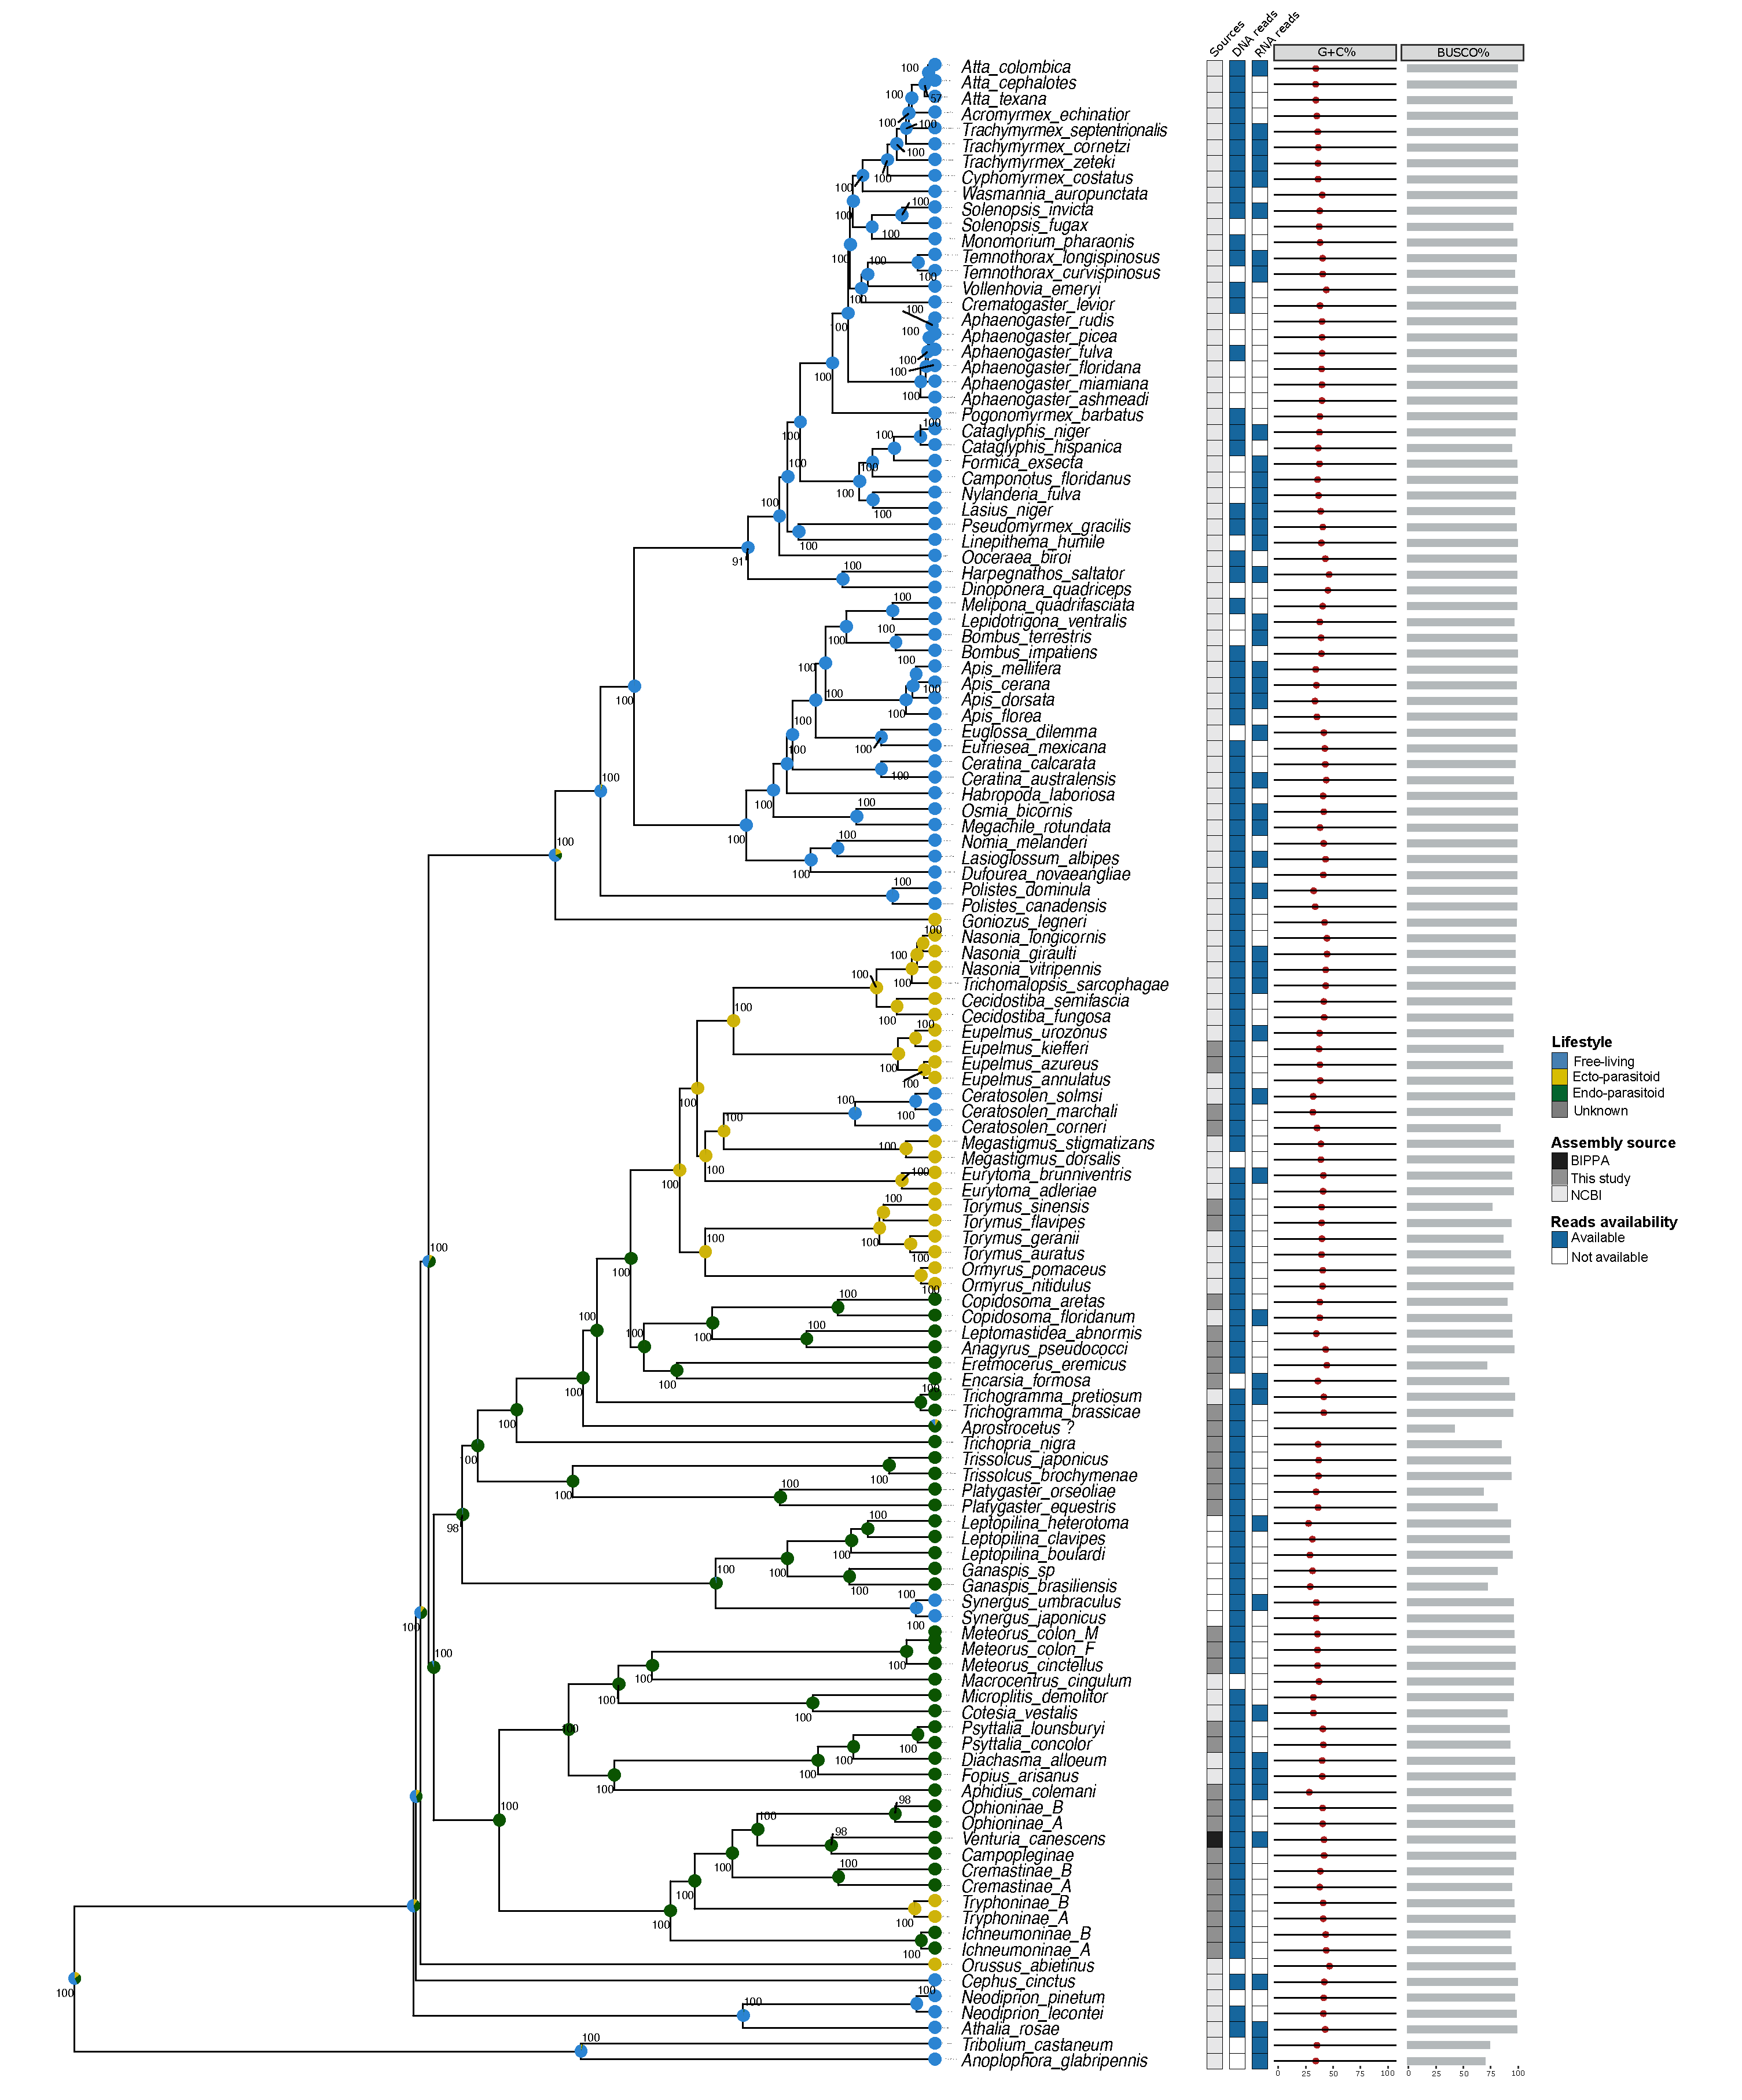
\includegraphics[width=\linewidth,height=\textheight,keepaspectratio]{PhD-master/figures/Genomes_qualities_and_origins.pdf}
\caption[Paper1:Genomic dataset sources]{\textbf{Source of the datasets and availability of the reads}. Phylogeny of 124 Hymenoptera species. Two Coleoptera species were used to root the tree. The aLRT bootstrap scores are represented along the nodes. The sources refer to the platform or laboratory in which the assemblages come from (This study, BIPPA: BioInformatics Platform for Agroecosystem Arthropods, NCBI: National Center for Biotechnology Information). The assemblies for which raw DNAseq or RNAseqs reads were available are listed in the column DNA or RNA reads. The G+C\% column reflects the average G+C rate for each assembly, and the BUSCO\% column reflects the rate of complete or partial BUSCOs found via the analysis with BUSCO V3. Posterior Bayesian lifestyle inference distribution for each node and tips  are represented by colored pie charts. }
\label{figure:Genomes_qualities_and_origins}
\end{figure}

\begin{figure}[H]
 \centering
  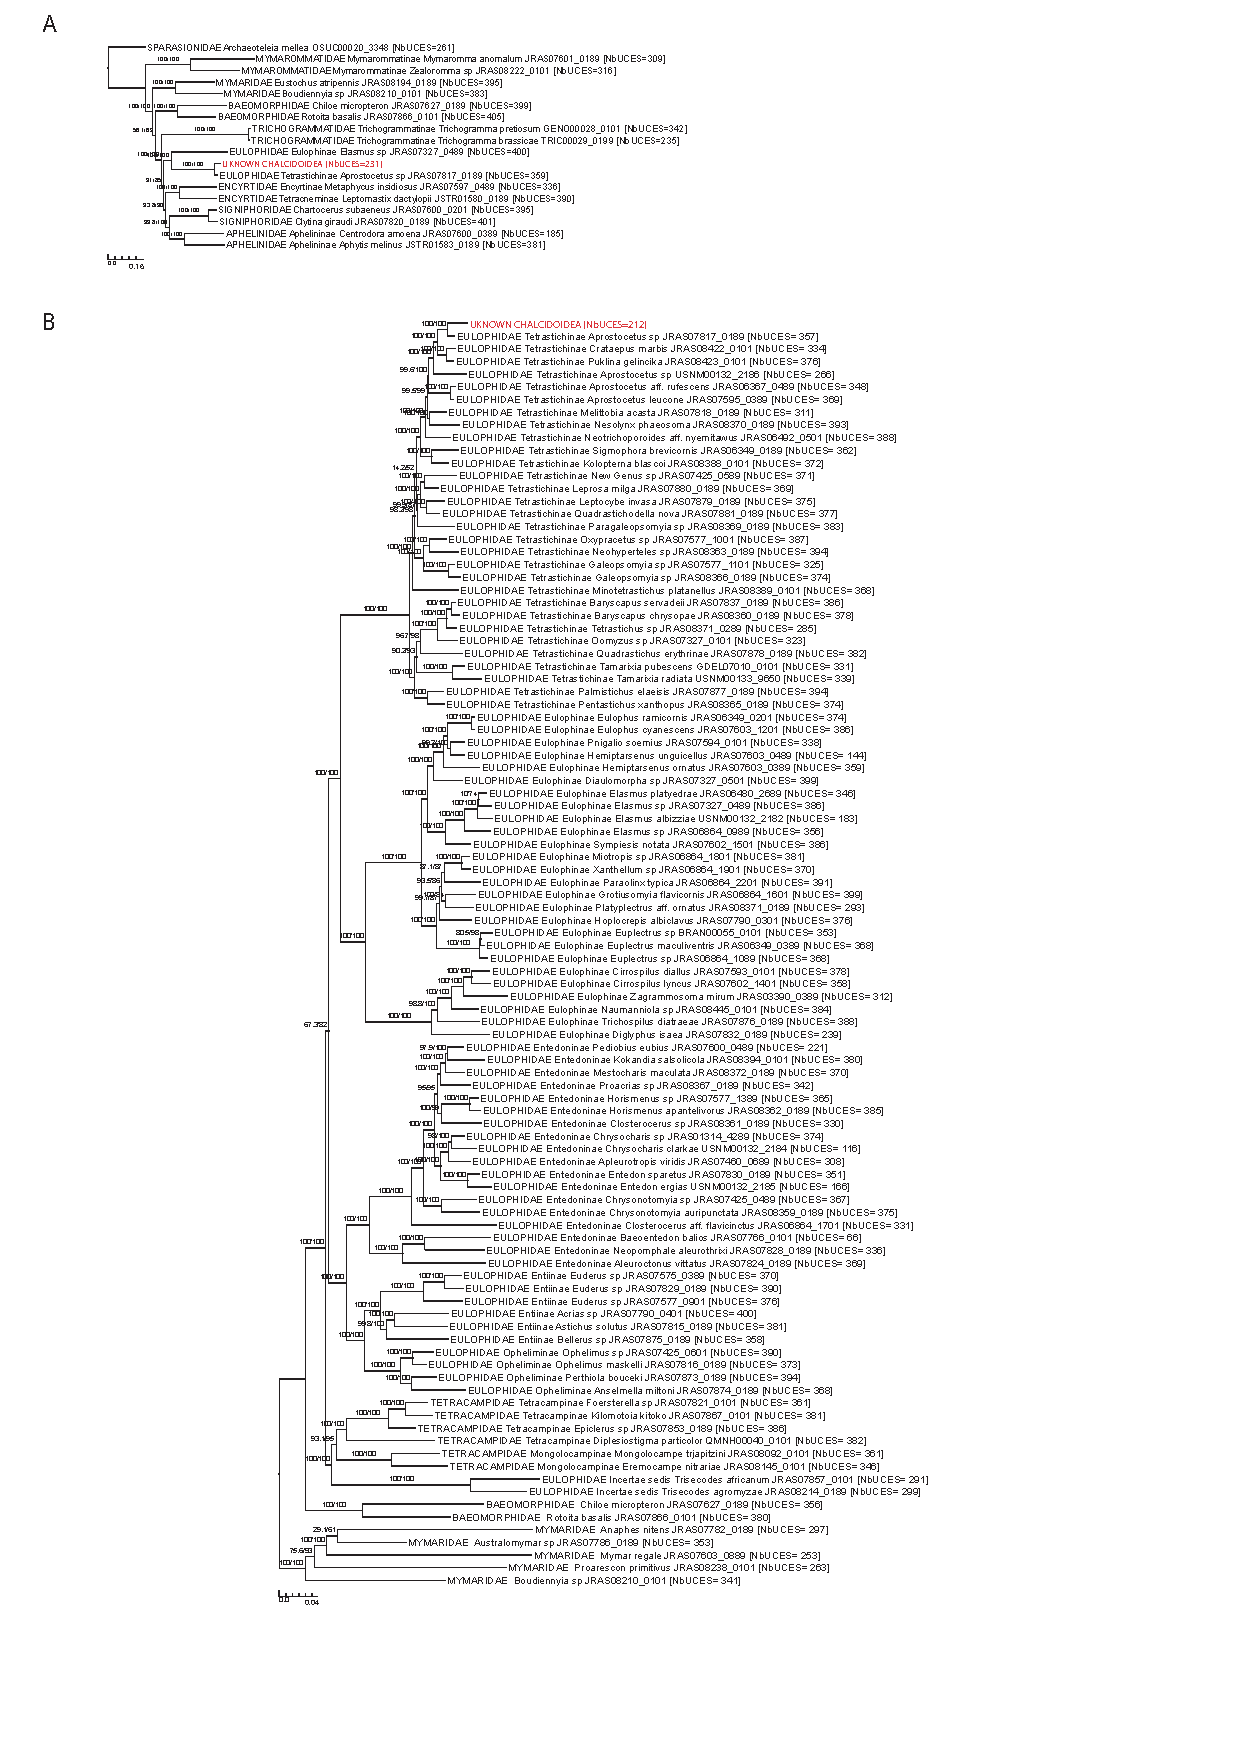
\includegraphics[width=\linewidth,height=\textheight,keepaspectratio]{PhD-master/figures/UCEs.pdf}
\caption[Paper1:UCE phylogenies to describe the unknown scaffolds]{\textbf{UCE trees built to assign to species the unknown Chalcidoidea sequenced with the pool of \textit{P. orseoliae}}. \textbf{A}: Phylogeny of early diverging families of Chalcidoidea (423 UCES and 127,979 bp were analysed to get the tree, best fit model = GTR+F+R10). \textbf{B} : Phylogeny of the family Eulophidae to which the unknown sample was inferred to belong to (408 UCES and 77,514 bp were analysed to get the tree, best fit model = GTR+F+R10). For both trees, SH-aLRT/UFBoot are shown at nodes; the number of UCEs analyzed for each sample is indicated between bracket and the unknown sample is highlighted in red.}
\label{figure:UCEs}
\end{figure}


\begin{table}[H]
\centering
\setlength{\extrarowheight}{0pt}
\addtolength{\extrarowheight}{\aboverulesep}
\addtolength{\extrarowheight}{\belowrulesep}
\setlength{\aboverulesep}{0pt}
\setlength{\belowrulesep}{0pt}
\caption[Paper1:Control table]{\textbf{Summary statistics for control cases}. The numerator indicates the numbers of EVEs or dEVEs inferred by our pipeline, and the denominator indicates the number of known EVEs for each case.  Analysis on \textit{dN/dS} was only possible when orthologs or paralogs were available.  Controls Endogenous viral elements present in scaffolds probably belonging to the Hymenoptera genome are scored from A to D, and scaffolds probably belonging to free viruses are scored as F or X: (see details in \hyperref[sec:MM-5]{Materials and methods}). TPM (Transcripts per kilobase million) values were calculated via RNAseq read mapping when available in the databases (all RNAseq data sources can be found on the GitHub file : \href{https://github.com/BenjaminGuinet/PhD_defense/blob/main/Supplementary_paper1/RNA_seq_reads_mapped.txt}{RNA\_seq\_reads\_mapped.txt}). * In addition to the expected unique shared event concerning the \textit{M. demolitor} and \textit{C. vestalis} species, our pipeline inferred two additional events, each specific to one lineage. This was due to the fact that two genes were not detected by our pipeline as shared by \textit{M. demolitor} and \textit{C. vestalis}, either because they are effectively not shared (for 3 of them: HzNVorf118, like-\textit{pif-4} (\textit{19kda}), \textit{fen-1}), or because of some false negative in one of the two lineage (for one of them:p33 (ac92)). }
\resizebox{\linewidth}{!}{%
\begin{tabular}{>{\hspace{0pt}}m{0.13\linewidth}|>{\hspace{0pt}}m{0.109\linewidth}|>{\hspace{0pt}}m{0.091\linewidth}|>{\hspace{0pt}}m{0.089\linewidth}>{\hspace{0pt}}m{0.106\linewidth}|>{\hspace{0pt}}m{0.089\linewidth}>{\hspace{0pt}}m{0.113\linewidth}>{\hspace{0pt}}m{0.089\linewidth}|>{\hspace{0pt}}m{0.08\linewidth}} 
\toprule
 & \textit{V. canescens} & \textit{F. arisanus} & \textit{C. vestalis} & \textit{M. demolitor} & \textit{L. boulardi} & \textit{L. heterotoma} & \textit{L. clavipes} & \% Total \\ 
\hhline{--------~}
{\cellcolor[rgb]{0.914,0.918,0.925}}\textbf{NB EVEs\footnotemark} & {\cellcolor[rgb]{0.914,0.91,0.918}}\textbf{36/40~} & {\cellcolor[rgb]{0.914,0.91,0.918}}\textbf{42/47~} & {\cellcolor[rgb]{0.906,0.91,0.918}}\textbf{20/21} & {\cellcolor[rgb]{0.914,0.91,0.918}}\textbf{18/25~} & {\cellcolor[rgb]{0.914,0.91,0.918}}\textbf{12/13} & {\cellcolor[rgb]{0.914,0.91,0.918}}\textbf{12/13} & {\cellcolor[rgb]{0.914,0.91,0.918}}\textbf{12/13~} & \textbf{88.4\%} \\
Scaffold A & 36  & 42  & 18 & 16 & 11 & 6 & 8  & 90.13\% \\
Scaffold B & 0 & 0 & 0 & 0 & 0~ & 0~ & 0 & 0\% \\
Scaffold C & 0 & 0 & 0 & 0 & 1 & 6 & 4  & 7.24\%  \\
Scaffold\textasciitilde{} D & 0 & 0 & 2 & 2 & 0 & 0 & 0 & 2.63\% \\
Scaffolds E-F-X & 0 & 0 & 0 & 0 & 0 & 0 & 0 & 0\% \\ 
\hhline{--------~}
{\cellcolor[rgb]{0.914,0.91,0.918}}\textbf{NB dEVEs} & {\cellcolor[rgb]{0.914,0.91,0.918}}\textbf{22/36~} & {\cellcolor[rgb]{0.914,0.91,0.918}}\textbf{11/42} & {\cellcolor[rgb]{0.922,0.914,0.925}}\textbf{20/20} & {\cellcolor[rgb]{0.914,0.91,0.918}}\textbf{18/18} & {\cellcolor[rgb]{0.914,0.91,0.918}}\textbf{12/12} & {\cellcolor[rgb]{0.914,0.91,0.918}}\textbf{12/12} & {\cellcolor[rgb]{0.914,0.91,0.918}}\textbf{12/12~} & \textbf{71.82\%} \\
by \textit{dN/dS}\footnotemark & 3/3 & 0/1 & 16/20 & 15/18  & 12/12 & 12/12 & 12/12  & 70.39\% \\
by TPM   1000 & 21 & 11 & 10 & 9  & 1 & 0 & 0 & 43.60\% \\
\hhline{--------~}
{\cellcolor[rgb]{0.898,0.894,0.902}}\textbf{Nb Events} & {\cellcolor[rgb]{0.898,0.894,0.902}}\textbf{1/1} & {\cellcolor[rgb]{0.898,0.894,0.902}}\textbf{1/1} & \multicolumn{2}{>{\centering\hspace{0pt}}m{0.195\linewidth}|}{{\cellcolor[rgb]{0.937,0.933,0.941}}\textbf{3/1*}} & \multicolumn{3}{>{\centering\hspace{0pt}}m{0.291\linewidth}|}{{\cellcolor[rgb]{0.929,0.922,0.933}}\textbf{1/1}} & . \\
\bottomrule
\end{tabular}}
%\raggedright{1 The total percentage is the average of the averages of the percentages found in each of the 4 events \footnotetext[1]{}}
\\\raggedright{1 When paralogs were detected on different scaffolds, the best scaffold score was used.\footnotetext[1]{}}
\\2 Analysis on \textit{dN/dS}was only possible when orthologs or paralogs were detected (for example, in \textit{V. canescens} this calculation was only possible for 3 genes having paralogs)\footnotetext[2]{}
\label{tab:Control_table}
\end{table}


% \usepackage{array}
% \usepackage{graphicx}
% \usepackage{booktabs}
% \usepackage{colortbl}


\begin{table}
\centering
\captionsetup{font=footnote}
\caption[Paper1:Summary table with all EVEs statistics]{
\textbf{Summary table}. Clusters refers to the number of homologous clusters with one or more candidate Endogenous Viral Elements (EVEs). Raw EVEs is the raw number of EVEs (i.e. including all paralogs and orthologs) according to the scaffold categories from A to D.
Nb EVEs with complete ORFs corresponds to the number of raw EVEs with an ORF starting with a methionine, without premature stop codons, and ending with a stop codon, distinguishing ORFs whose size is at least equal to or greater than 80\% of that of the best viral hit. 
EVEs is the count of EVEs, i.e. counting the number of genes within each monophyletic group only once (as several EVEs may have undergone post-endogenization duplications or an EVE may be ancestrally acquired and shared by several species). Mean pident is the average of the percentage identity of all EVEs with the best viral hit, the number in brackets corresponds to the standard error. Nb EVEs pident and Nb EVE E-values 1e-20 correspond to the number of refined EVEs showing a hit with more than 80\% identity and an E-value below  1e-20 with a viral protein, respectively. 
Domesticated EVEs (dEVEs) corresponds to the number of refined EVEs with either a \textit{dN/dS} significantly less than 1 with a complete ORF and without a stop codon and/or a TPM value $>$ 1000 with a complete ORF and without stop codon.
Events corresponds to the number of endogenization events that may include one or more genes and involve one or more species. Shared Events is the number of endogenization events shared by at least two species. Viral families corresponds to the number of different putative viral families associated with the best viral hits.  dEvents corresponds to the number of endogenization events presenting at least one dEVE.}
\setlength{\extrarowheight}{0pt}
\addtolength{\extrarowheight}{\aboverulesep}
\addtolength{\extrarowheight}{\belowrulesep}
\setlength{\aboverulesep}{0pt}
\setlength{\belowrulesep}{0pt}
\resizebox{\linewidth}{!}{%
\begin{tabular}{>{\hspace{0pt}}m{0.223\linewidth}>{\hspace{0pt}}m{0.174\linewidth}>{\hspace{0pt}}m{0.129\linewidth}>{\hspace{0pt}}m{0.131\linewidth}>{\hspace{0pt}}m{0.14\linewidth}>{\hspace{0pt}}m{0.107\linewidth}} 
\toprule
 & dsDNA & ssDNA & dsRNA & ssRNA & Total \\ 
\hline
Clusters & 166 & 9 & 18 & 36 & 229 \\ 
\hline
Raw EVEs \par{}(A\textbar{}B\textbar{}C\textbar{}D) & 819\par{}(534\textbar{}61\textbar{}102\textbar{}122) & 92\par{}(40\textbar{}27\textbar{}6\textbar{}19) & 95\par{}(45\textbar{}19\textbar{}26\textbar{}5) & 255\par{}(129\textbar{}74\textbar{}34\textbar{}18) & 1261 \\
Complet raw EVEs ORFs\par{}($>$80\% best viral hit) & 694 (409) & 74 (39) & 76 (26) & 223 (76) & 1067 (550) \\
\rowcolor[rgb]{0.91,0.91,0.91} EVEs & 366 & 32 & 61 & 162 & 621 \\
Mean pident (sd) & 36.99 (15.35) & 36.91 (11.37) & 38.32 (13.27) & 33.30 (11.82) & 36.32 \\
EVE pidents$>$>= 80 & 22 & 0 & 0 & 0 & 22 \\
EVE E-values  1e-20 & 430 & 29 & 67 & 126 & 652 \\
dEVEs & 112 & 9 & 12 & 38 & 171 \\
\rowcolor[rgb]{0.91,0.906,0.91} Events & 130 & 26 & 59 & 152 & 367 \\
shared Events & 17 & 1 & 5 & 13 & 36 \\
viral families/clades & 12 & 3 & 4 & 21 & 40 \\
dEvents & 47 & 10 & 12 & 38 & 107 \\
\bottomrule
\end{tabular}
}
\label{tab:Summary_candidate_numbers}
\end{table}


\begin{figure}[!htpb]
\captionsetup{font=footnotesize}
 \centering
  \includegraphics[width=\linewidth,height=\textheight,keepaspectratio]{PhD-master/figures/Cluster21304_AA.dna.treefile.pdf}
\caption[Paper1:Canonical example of an endogeniation events]{\textbf{Example of endogenization events}. The phylogeny of cluster21304 corresponds to the clustering of a set of viral and candidate viral insertion genes sharing a homology. In red are represented the loci of viral origin, and in blue are represented the loci probably endogenized (EVEs). The letter at the end of the taxon label represents the endogenization score assigned to the candidate (see details in \hyperref[sec:MM-5]{Materials and methods}). In this example, we found two singular endogenization events in the species endoparasitoid \textit{Encarsia formosa} (annotated A and thus presenting a depth of coverage non-significantly different from the distribution of the BUSOs of the genome as well as at least one transposable element and/or one eukaryotic gene) and ectoparasitoid \textit{Torymus auratus} (annotated C and thus presenting only a depth of coverage non-significantly different from the distribution of the BUSOs of the genome). Since these two species do not share a close common ancestor in the phylogeny and come from two different families, the algorithm therefore assigned them to two independent viral endogenization events. The viral locus found in the assembly of the endoparasitoid species \textit{Platygaster orseoliae} was annotated F, meaning that the depth of coverage deviated significantly from the BUSCO distribution of the genome and that no TEs and less than 5 eukaryotic genes were found in the scaffold containing the candidate insertion. Finally, the two loci belonging to the ectoparasitoid species \textit{Megastigmus stigmantizans} and \textit{Megastigmus dorsalis} both show a score supporting viral endogenization. Furthermore, these species exhibit a doubly monophyletic clade (high bootstrap score) within the gene phylogeny and within the species phylogeny, suggesting that they acquired this viral gene from their closest common ancestor about 20 million years ago. All newick phylogenies are available on the GitHub file : \href{https://github.com/BenjaminGuinet/PhD_defense/blob/main/Supplementary_paper1/All_cluster_phylogenies_merged.pdf}{All_cluster_phylogenies_merged.pdf}.}
\label{figure:Cluster21304_phylogeny_example}
\end{figure}


\begin{figure}[!htpb]
\captionsetup{font=footnotesize}
 \centering
    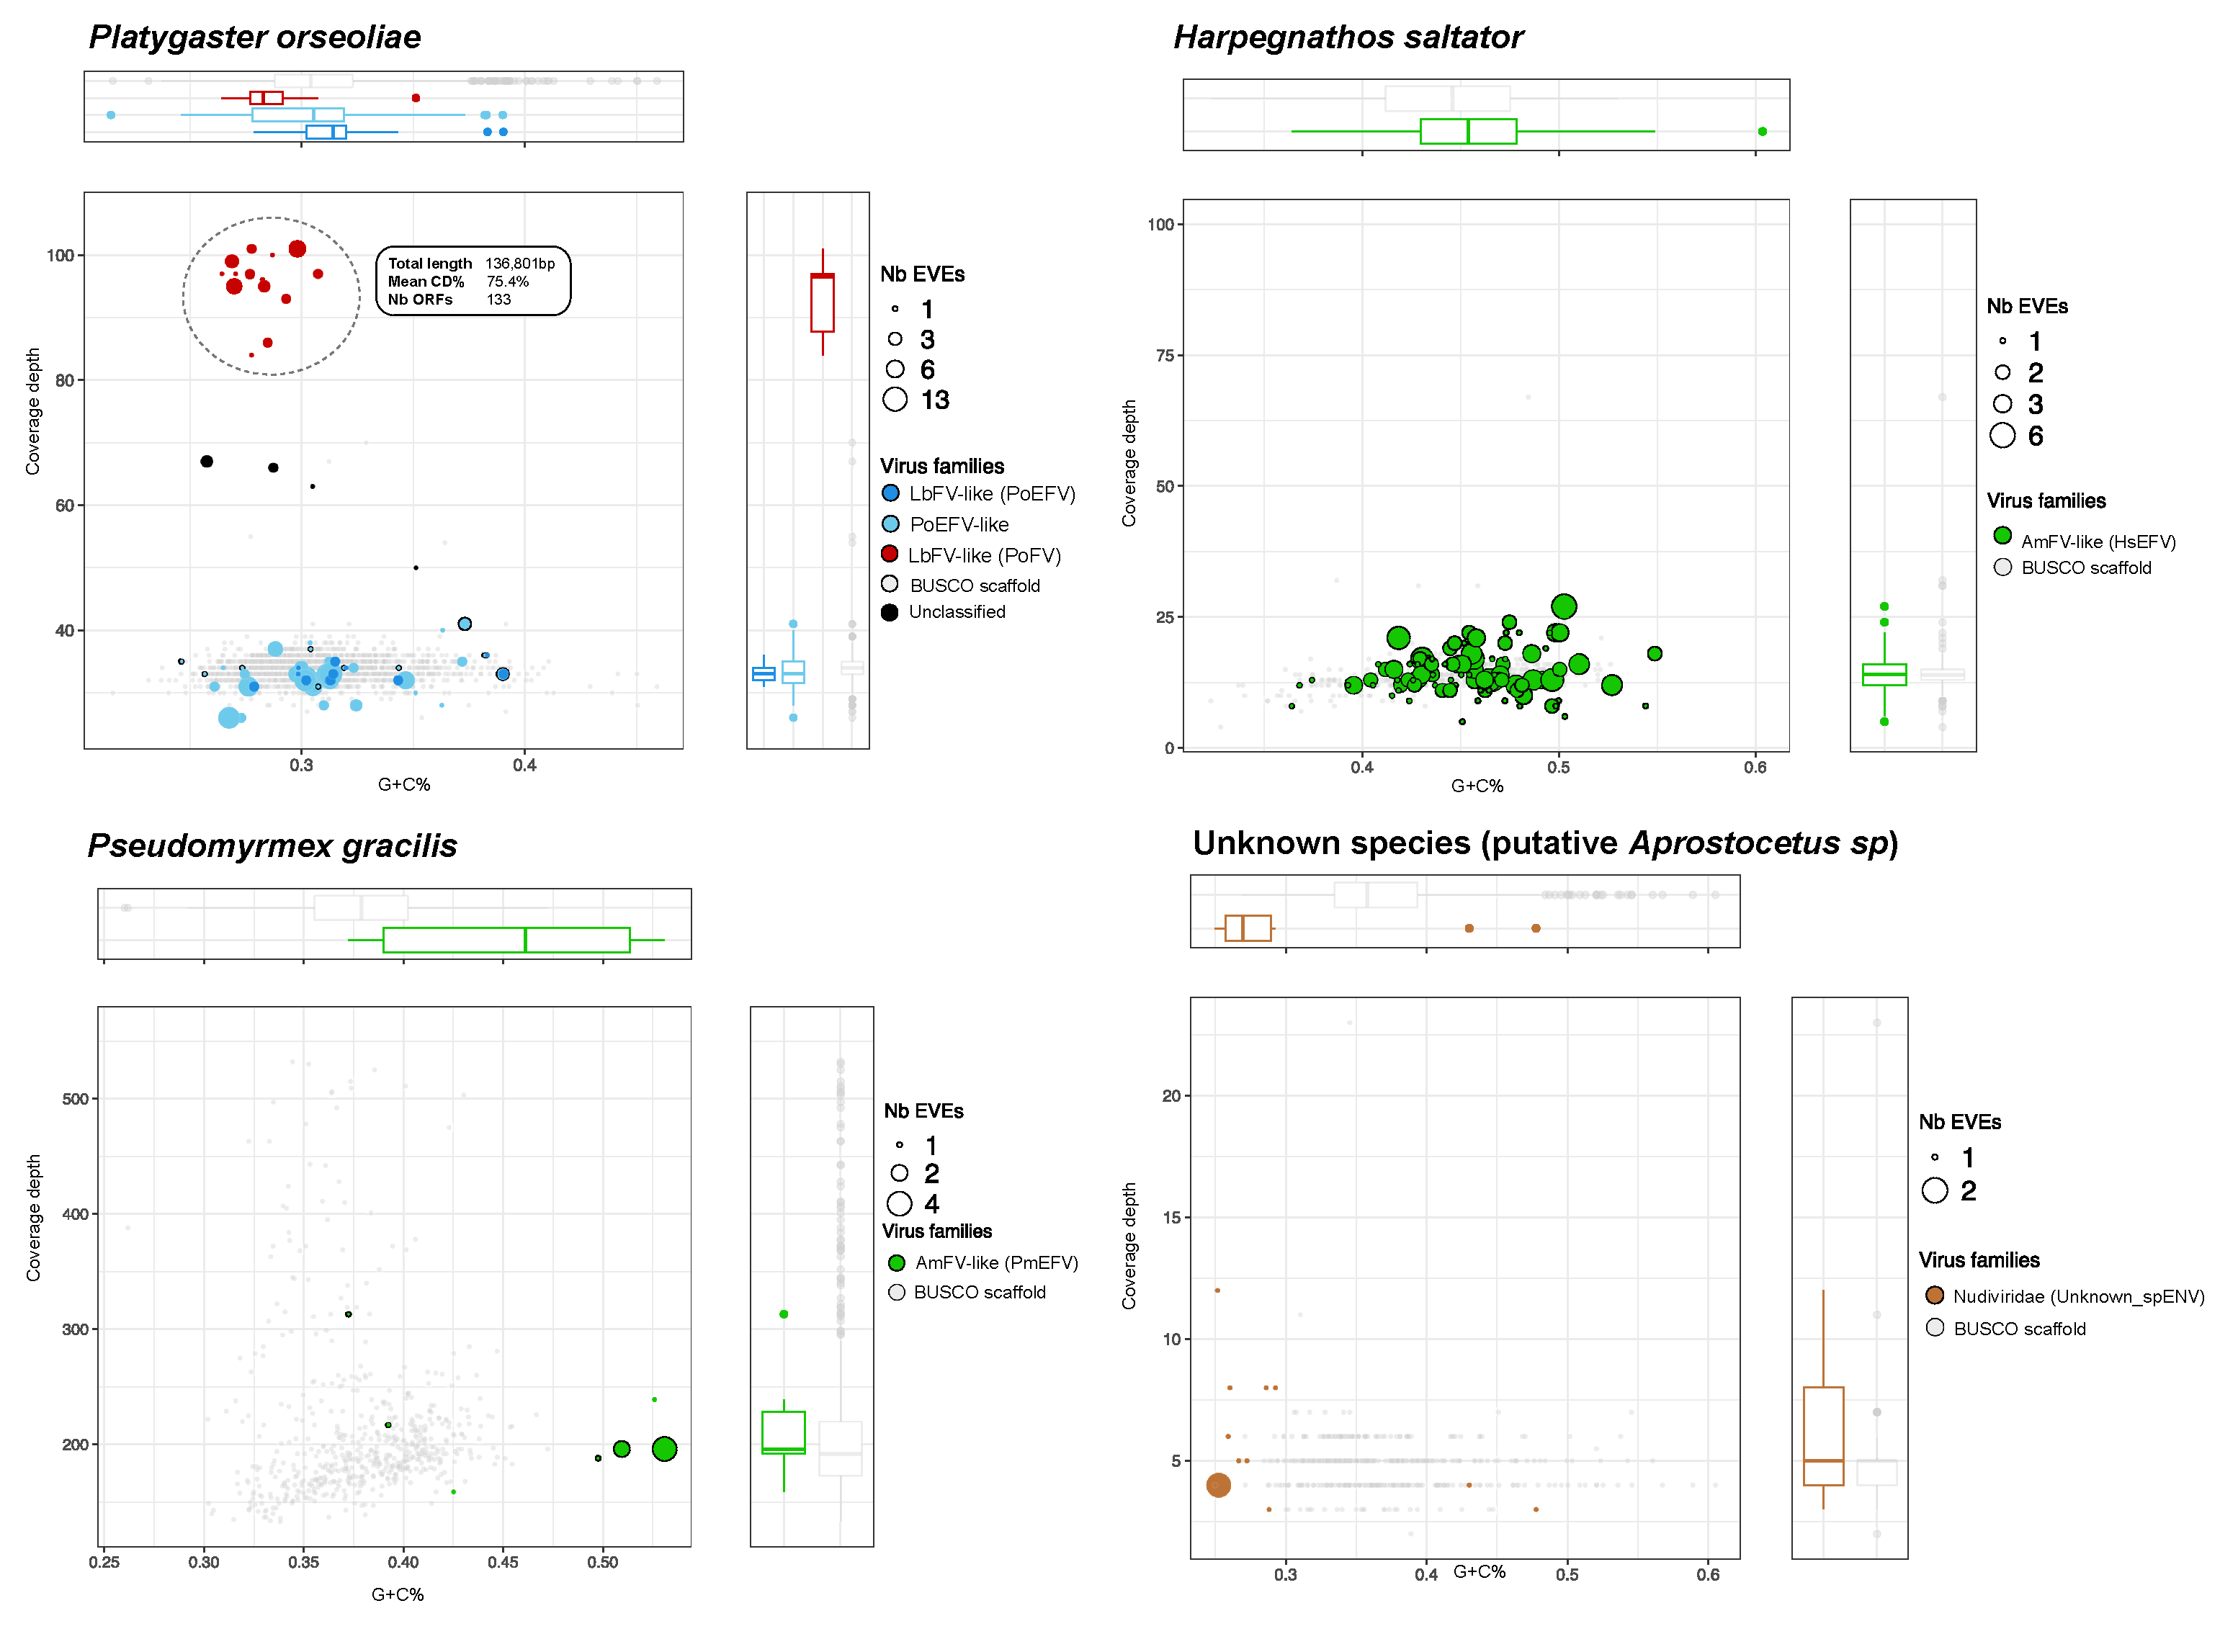
\includegraphics[width=\linewidth,height=\textheight,keepaspectratio]{PhD-master/figures/Multiple_EVEs_COV_GC.pdf}
\caption[Paper1:GC and coverage distribution of scaffolds containing multiple EVEs Events]{\textbf{G+C\%Coverage distribution of scaffold containing multiple EVEs Events}.  The size of the dots corresponds to the number of candidate EVEs inside the scaffold. The color represents the genomic entity from which the EVE probably originated (brown: \textit{Nudiviridae}, blue = LbFV and green = AmFv). The red color refers to scaffolds showing free-living virus signatures. The grey color refers to scaffolds containing one or more BUSCO genes. The dots circled in black correspond to scaffolds that contain one or more eukaryotic genes and/or repeat elements.}
\label{figure:Multiple_EVEs_COV_GC}
\end{figure}


\begin{figure}[!htbp]
\captionsetup{font=footnotesize}
 \centering
  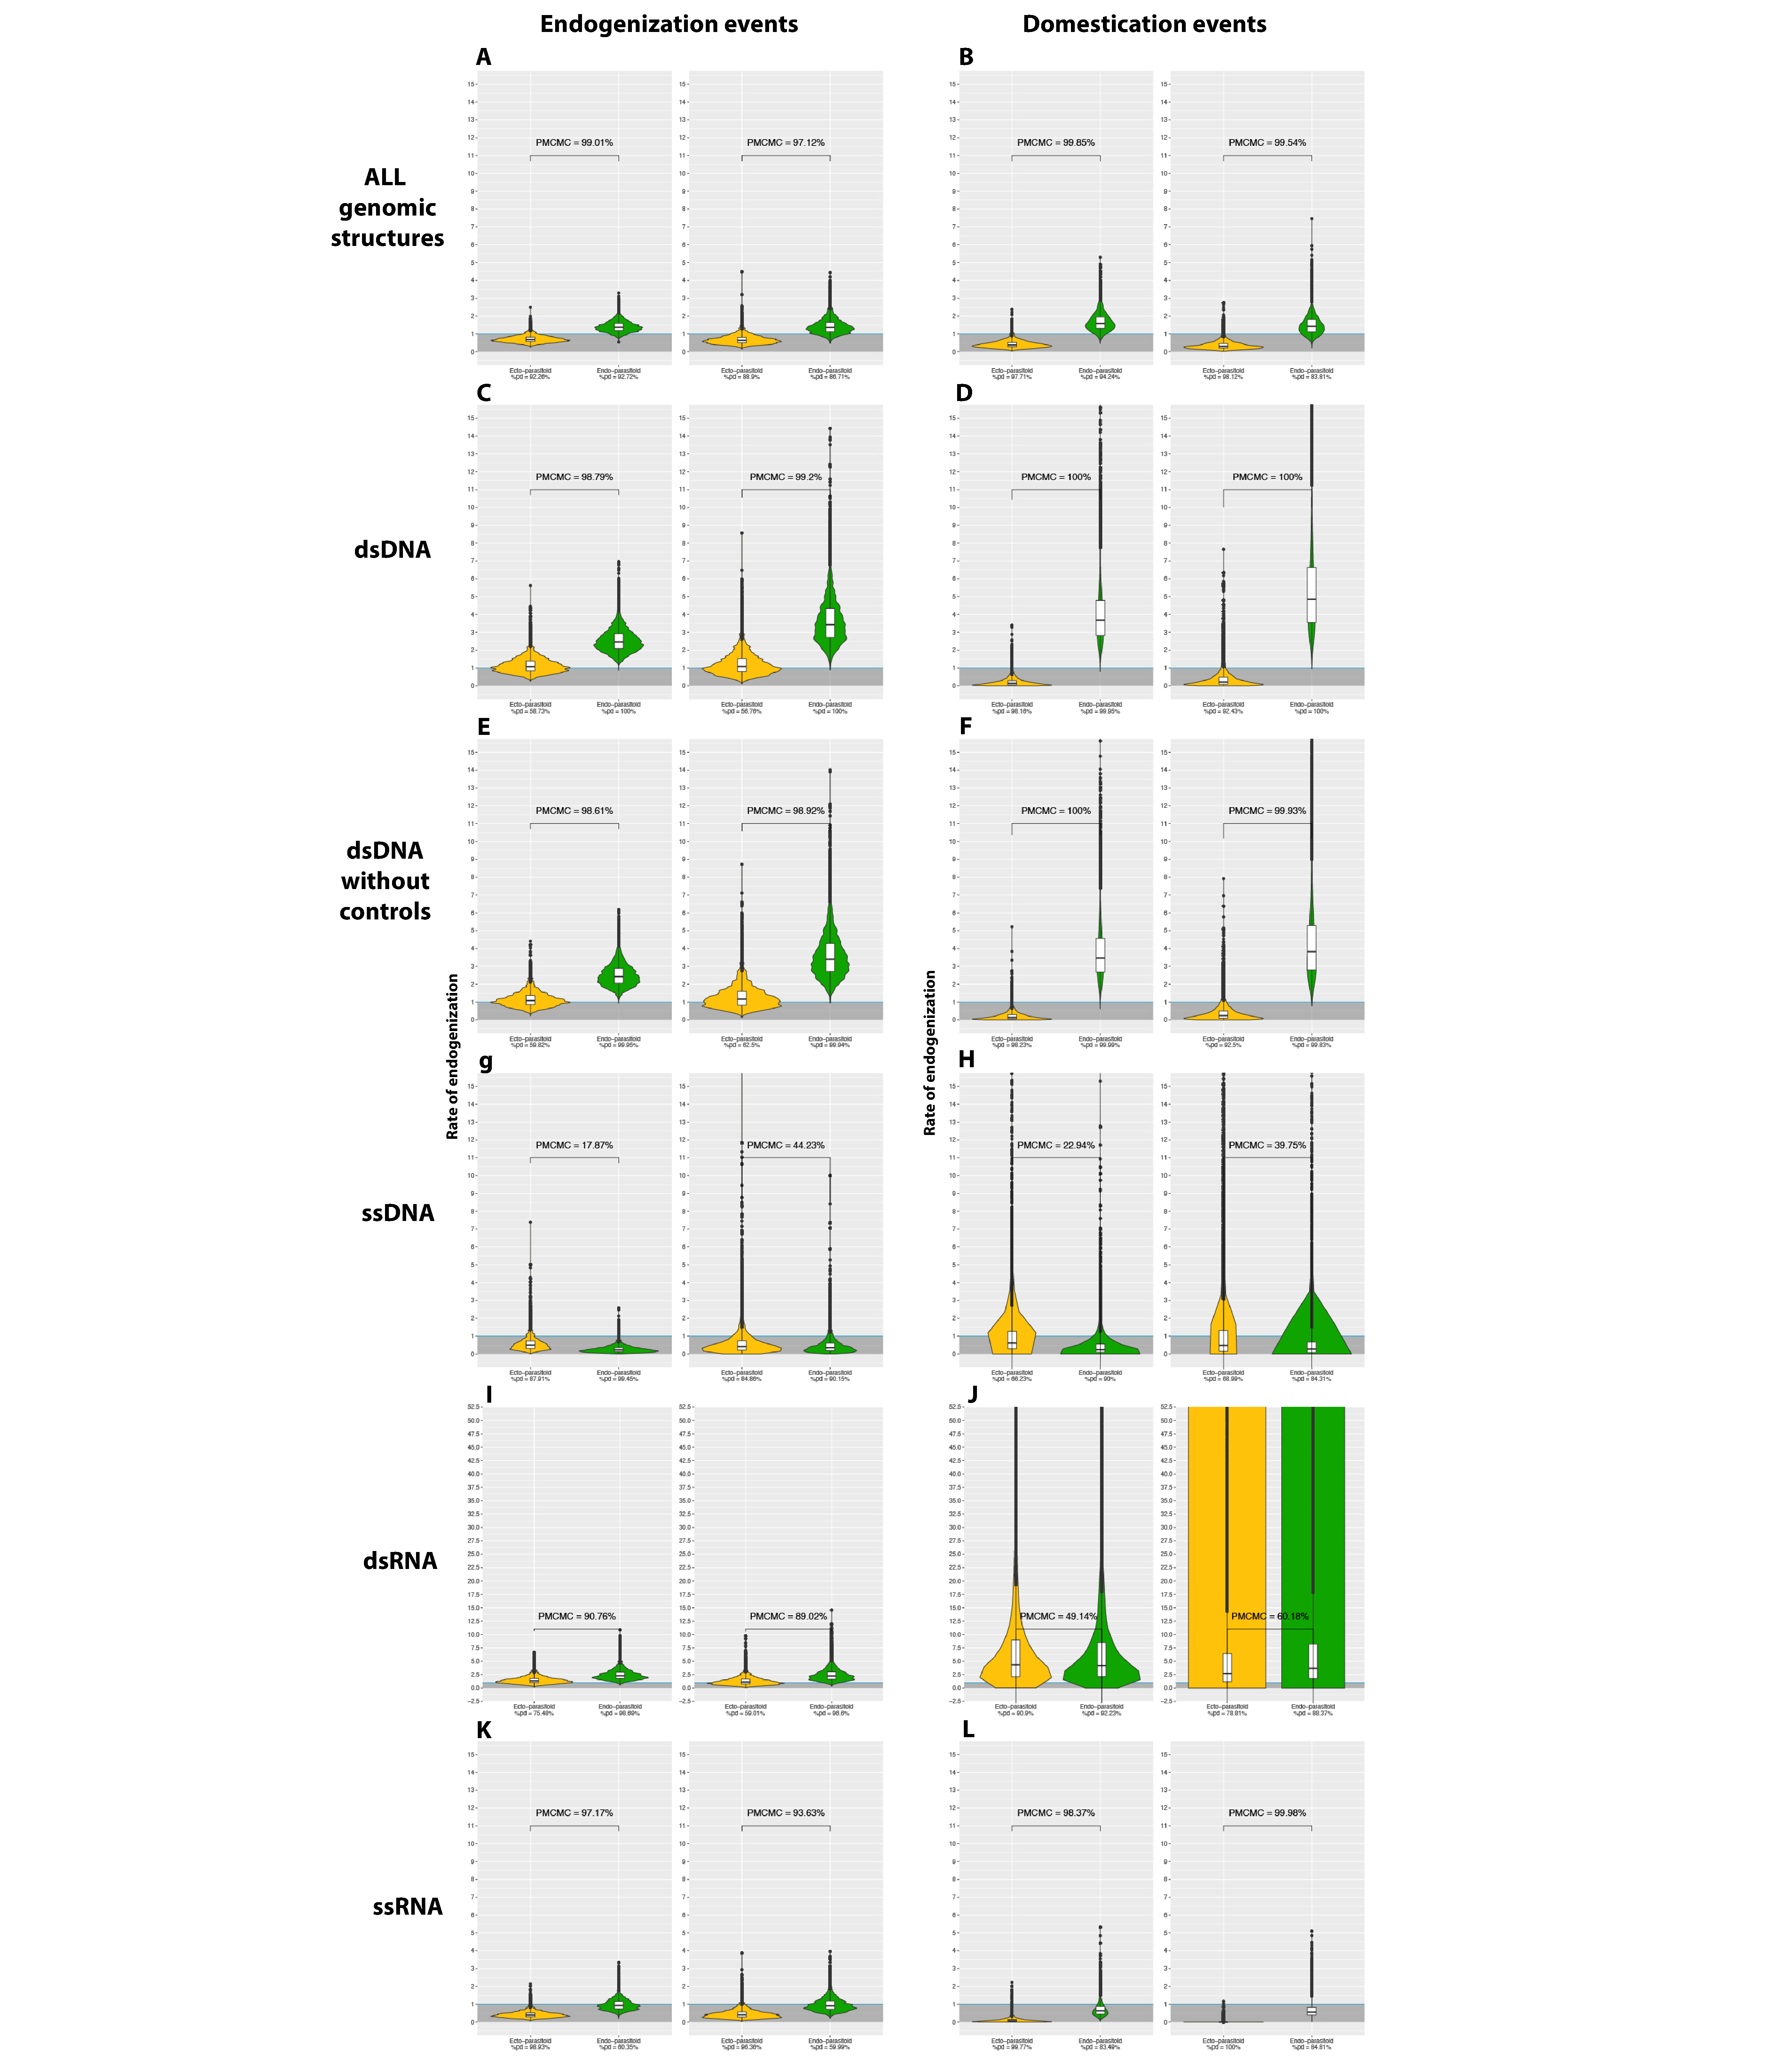
\includegraphics[width=\linewidth,height=\textheight,keepaspectratio]{PhD-master/figures/All_violin_plots_new_order2.pdf}
\caption[Paper1:Violon plot distribution of GLM coefficients of EVEs,dEVEs,Events and dEvents for each genomic viral structure]{\textbf{Violin plots of the posterior distribution of GLM coefficients after exponential transformation in relation to wasp lifestyle}. The ectoparasitoid lifestyle is in yellow, the endoparasitoid lifestyle is in green, and the free-living lifestyle is in blue. Coefficients have been transformed into exponential and correspond to the posterior distribution of the coefficients of a binomial negative zero-inflated GLM model, where the lifestyle free-living stand for the intercept. The Y-axis corresponds to the multiplicative factor of the number of endogenization and/or domestication of EVES and/or events relative to free-living species. The coefficients are derived from 1000 GLM models adjusted on 1000 randomly selected probable scenarios ($>$90 CI) of ancestral states at nodes. Branches from nodes older than 160 million years have been removed from the dataset. The ROPE\% is the percentage of the posterior distribution of coefficients below the intercept. The posterior distribution of the interaction coefficients between lifestyles and branch size were not informative, and the branch size factor was therefore added as an additive effect to the model.}
\label{figure:All_violin_plots}
\end{figure}


\begin{figure}[!htpbt]
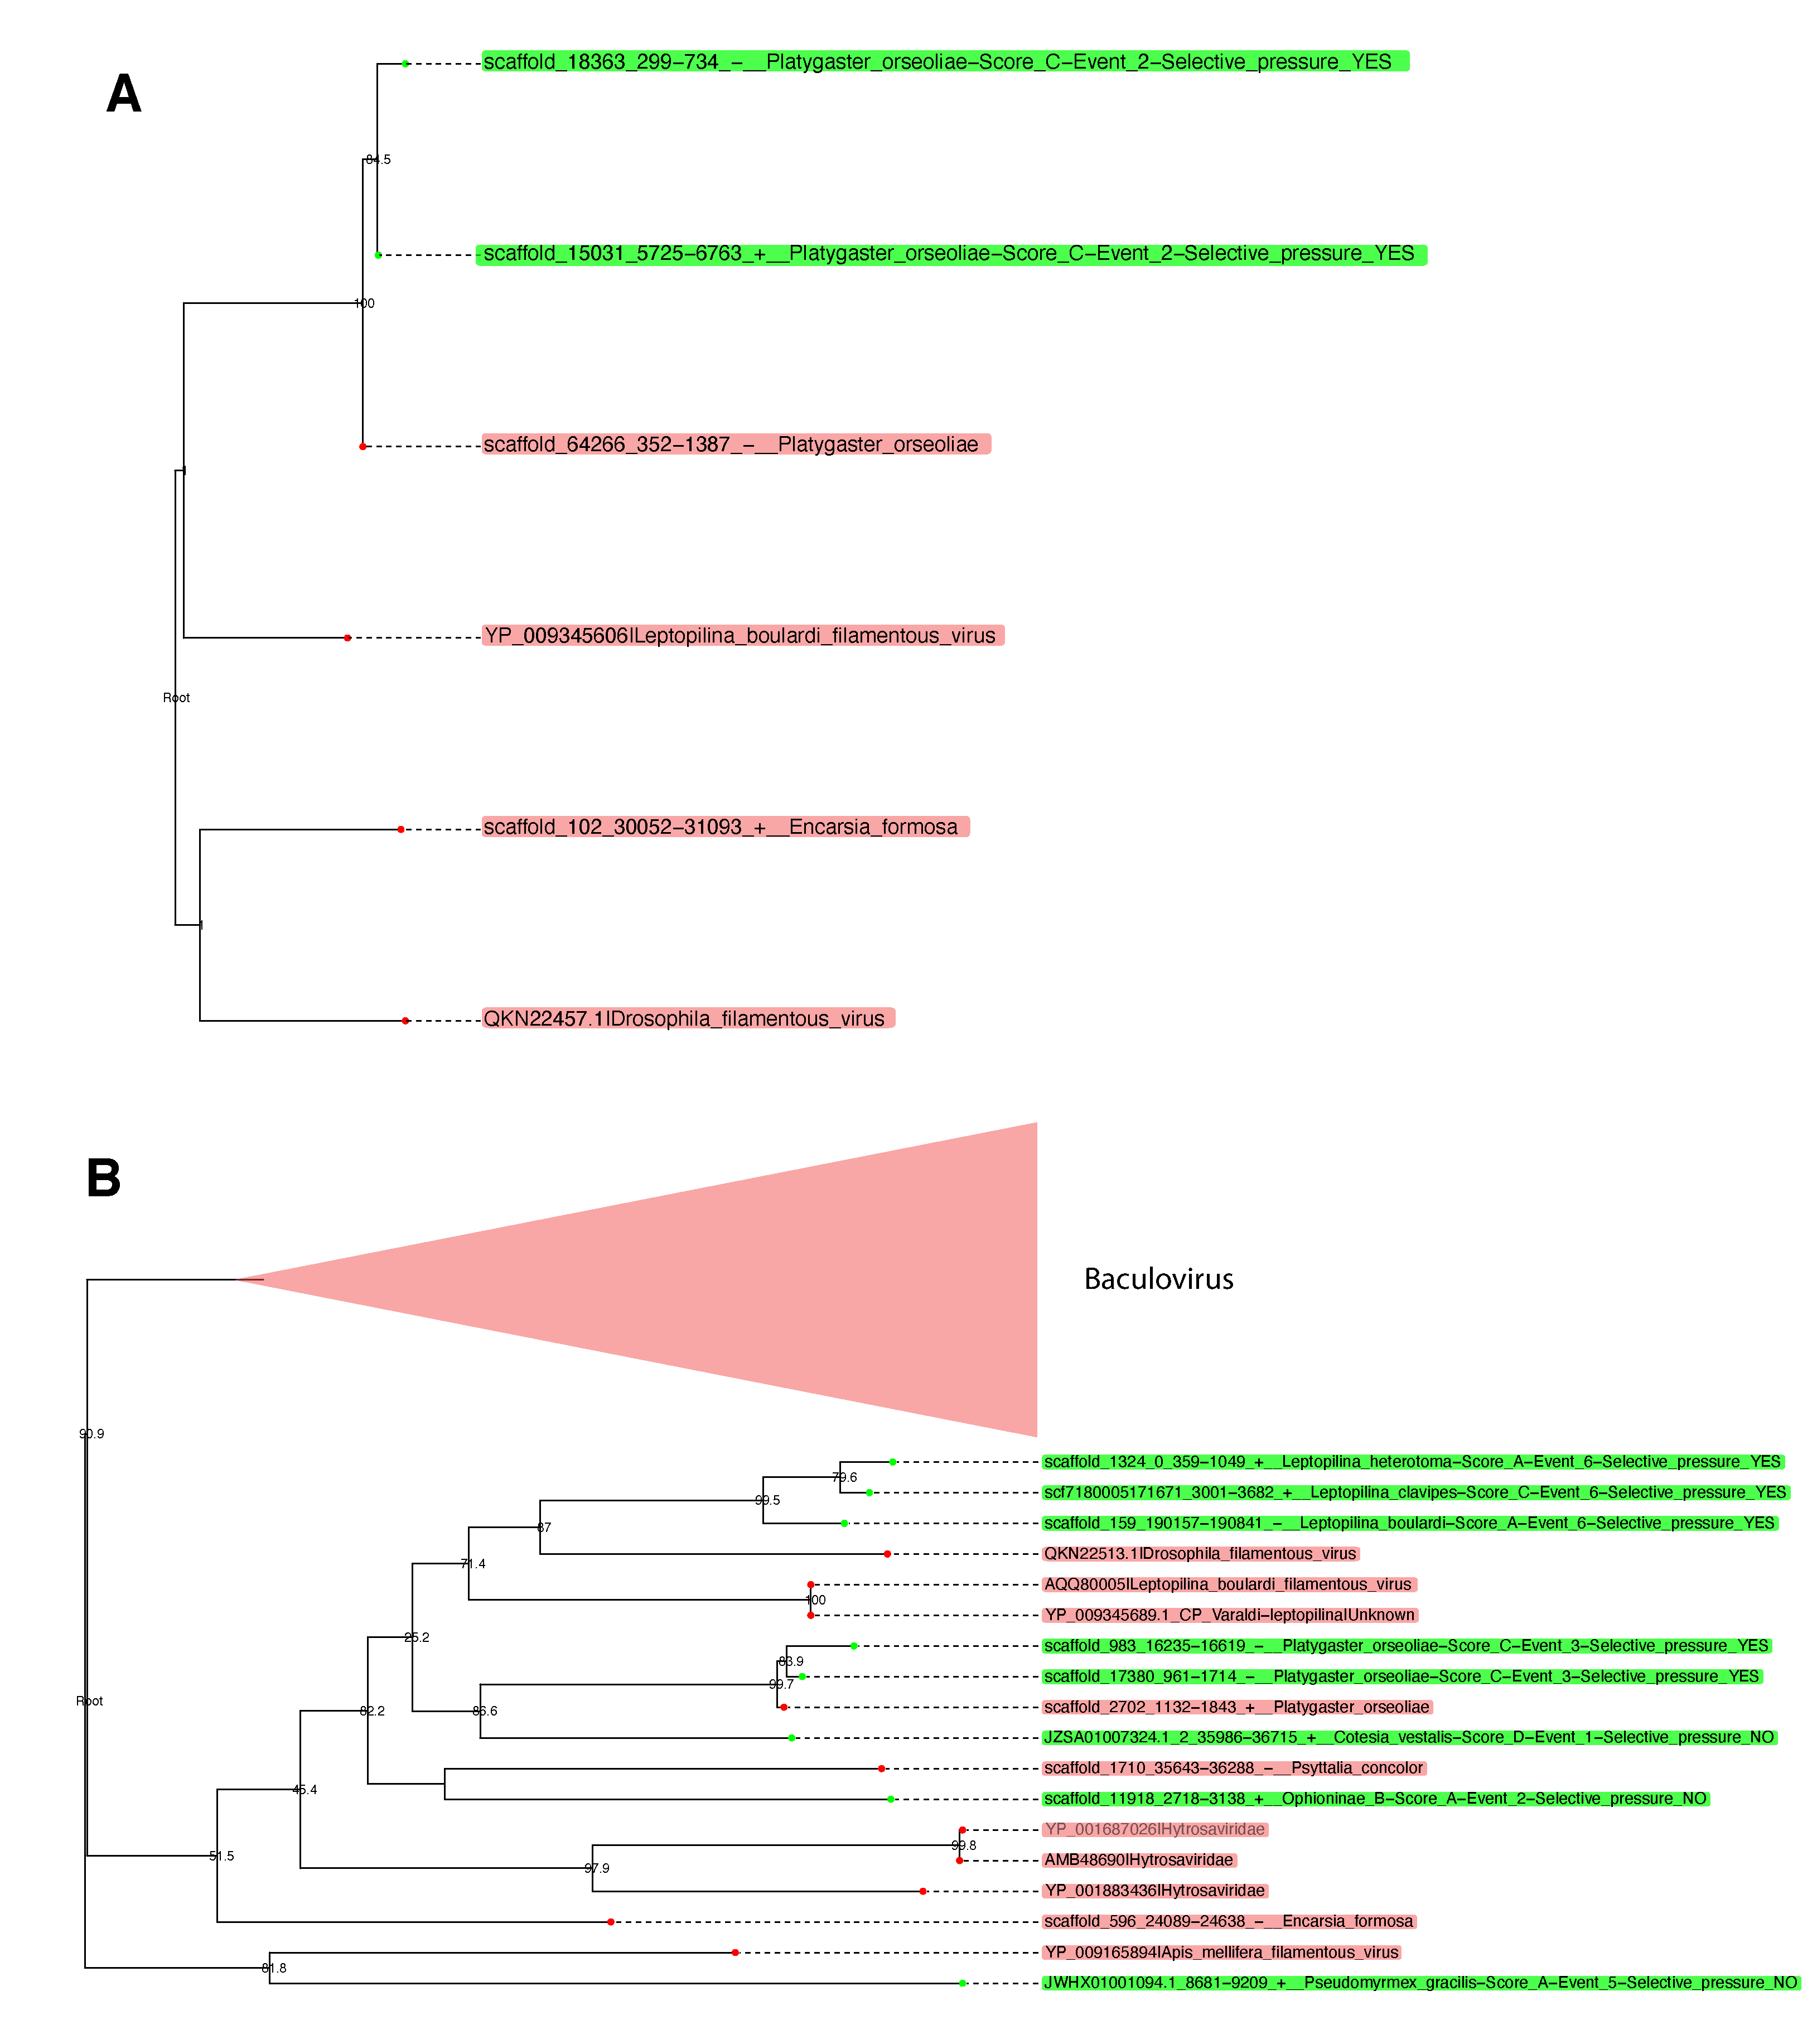
\includegraphics[width=\linewidth,height=\textheight,keepaspectratio]{PhD-master/figures/Porseoliae_LbFV-like_phylogenies.pdf}\centering
\caption[Paper1:\textit{P. orseoliae} integrase and Ac81 EVE phylogenies]{\textbf{Phylogenies of LbFV-like proteins under purifying selection in \textit{Platygaster orseoliae} genome}. The panel A represents the Cluster\_25710 which corresponds to the \textit{integrase} protein. The panel B represents the Cluster\_26675 which corresponds to the \textit{Ac81} protein. Taxa in red correspond to putative  loci belonging to free-living viruses, while green taxa correspond to putative EVEs (the assigned family is indicated after the pipe). Green labels indicate the following information : (1) scaffold name, (2) start location, (3) end location, (4) strand, (5) Hymenoptera species, (6) endogenization index, (7) the inferred event number within the cluster phylogeny, and (8) whether the loci are found under purifying selection (YES) or not (NO).}
\label{figure:Porseoliae_LbFV-like_phylogenies}
\end{figure}

%\begin{figure}[!htpbt]
%\includegraphics[width=\linewidth,height=\textheight,keepaspectratio]{GO_distribution_dEVEs_vs_freeliving_dsDNA_viruses.pdf}\centering
%\label{figure:EVE_dEVEs_sementic_spaces_comparison}
%\caption{\textbf{Semantic space distribution of typical dsDNA viral Go terms compared to endoparasitoid candidate EVEs Go terms}.  The GO terms semantic space distribution of dsDNA virus is based on the proteomes of 7 dsDNA viruses from 7 different families which were involved in more than one endogenization Event except for textit{Phycodnavirida}e. Red point mean that the same function is found within candidates and in the viral dsDNA GO terms repertoire. The size of the dots represents the proportion of the GO terms in the dsDNA virus repertoire. }
%\end{figure}

% \usepackage{array}
% \usepackage{graphicx}
% \usepackage{booktabs}


\begin{table}
\centering
\tiny
\caption[Paper1:RNA EVEs distribution along scaffolds]{\textbf{EVEs distribution according to putative non-segmented single-stranded RNA virus donor and their genomic position}. For each EVE, we retrieved the position of the homologous ORF in the virus genome identified after a blastp search (first hit). The information on the position of the ORFs was retrieved either from \cite{shi_redefining_2016}, from the ICTV reports or manually after recovery of the viral assembly in NCBI, ORF annotation with getorf (ORF length min= 150bp) and blastp to confirm the position of the ORFs and their functions. The position of the ORF in the free-living virus genome is reported in the column "ORF position", when the genome was incomplete, we inferred the position of the ORF with respect to the position of the homolog in the closest complete viral genome. The number of EVEs corresponds to the number of EVEs counting paralogs only once (i.e. counting only one EVE per species per gene cluster).}
\resizebox{\linewidth}{!}{%
\begin{tabular}{>{\hspace{0pt}}m{0.092\linewidth}>{\hspace{0pt}}m{0.179\linewidth}>{\hspace{0pt}}m{0.094\linewidth}>{\hspace{0pt}}m{0.24\linewidth}>{\hspace{0pt}}m{0.159\linewidth}>{\hspace{0pt}}m{0.088\linewidth}>{\hspace{0pt}}m{0.065\linewidth}} 
\toprule
Family & Closest viral blast hit & Protein ID & Protein Name & ORF position & Source & Nb EVEs  \\ 
\hline
\textit{Artoviridae} & Pteromalus puparum peropuvirus & YP\_009505431 & Glycosylated matrix protein M (U3) & 3 out 5 & ICTV & 19 \\
\textit{Artoviridae} & Pteromalus puparum peropuvirus & YP\_009505433 & RNA pol (L) & 5 out 5 & ICTV & 9 \\
\textit{Artoviridae} & Beihai rhabdo like virus 1 & YP\_009333442 & Phosphoprotein (U2) & 2 out 3 & ICTV & 1 \\ 
\hline
\textit{Bornaviridae} & Estrildid finch bornavirus 1 & YP\_009505428 & RNA pol (L) & 4 out
  4 & Manually & 8 \\ 
\hline
\textit{Chuviridae} & Hubei chuvirus like 1 & YP\_009337906 & Nucleoprotein (N) & Incomplete (putative 3 out 3) & Manually & 24 \\
\textit{Chuviridae} & Hubei coleoptera virus  3 & YP\_009336865 & Nucleoprotein (N) & 2 out 3 & Shi et al 2016 & 6 \\
\textit{Chuviridae} & Hubei chuvirus like 3 & YP\_009337091 & Nucleoprotein (N) & 3 out 3 & Shi et al 2016 & 2 \\
\textit{Chuviridae} & Hubei coleoptera virus 3 & YP\_009336866 & RNA pol (L) & 3 out 3 & Shi et al 2016 & 2 \\
\textit{Chuviridae} & Lonestar tick chuvirus & YP\_009254003 & Nucleoprotein (N) & 3 out 3 & Manually & 1 \\
\textit{Chuviridae} & Hubei odonate virus 11 & YP\_009336948 & Nucleoprotein (N) & 3 out 3 & Shi et al 2016 & 1 \\ 
\hline
\textit{Lispiviridae} & Tacheng tick virus 6 & YP\_009304417 & ORF1 & 1 out 5 & Manually & 5 \\
\textit{Lispiviridae} & Hubei rhabdo like virus 3 & YP\_009336884 & Glyceraldehyde-3-phosphate dehydrogenase & 1 out 5 & Manually & 7 \\
\textit{Lispiviridae} & Hubei rhabdo like virus 3 & YP\_009336887 & Glycoprotein (G) & 3 out 5 & Manually & 2 \\
\textit{Lispiviridae} & Hubei rhabdo like virus 3 & YP\_009336889 & RNA pol (L) & 5 out 5 & Manually & 1 \\ 
\hline
\textit{Nyamiviridae} & Midway nyavirus & YP\_002905336 & Nucleoprotein (N) & 1 out 6 & ICTV & 8 \\
\textit{Nyamiviridae} & Orinoco orinovirus & YP\_009666283 & Nucleoprotein (N) & 1 out 4 & Manually & 8 \\
\textit{Nyamiviridae} & Sierra Nevada nyavirus & YP\_009044206 & Nucleoprotein (N) & 1 out 6 & ICTV & 5 \\
\textit{Nyamiviridae} & Nyamanini nyavirus & YP\_002905342 & Nucleoprotein (N) & 1 out 6 & ICTV & 4 \\
\textit{Nyamiviridae} & Midway nyavirus & YP\_002905331 & RNA pol (L) & 6 out 6 & ICTV & 1 \\
\textit{Nyamiviridae} & Wenzhou Crab Virus 1 & YP\_009304556 & Nucleoprotein (N) & 1 out 4 & Manually & 1 \\
\textit{Nyamiviridae} & Beihai rhabdo like virus 3 & YP\_009666292 & RNA pol (L) & 5 out 5 & Shi et al 2016 & 1 \\ 
\hline
\textit{Rhabdoviridae} & Wugan Ant virus & YP\_009304559 & RNA pol (L) & Incomplete (putative 5 out 5) & Manually & 2 \\
\textit{Rhabdoviridae} & Wuhan insect virus 7 & YP\_009301743 & RNA pol (L) & 5 out
  5 & Manually & 1 \\
\textit{Rhabdoviridae} & Sanxia Water Strider Virus 5 & YP\_009289351 & Glycoprotein (G) & 4 out
  5 & Manually & 1 \\
\textit{Rhabdoviridae} & Muscina stabulans sigmavirus & YP\_009664711 & RNA pol (L) & Incomplete (putative 5 out 5)  & Manually & 1 \\
\bottomrule
\end{tabular}
}
\label{tab:single-stranded_RNA_orf_location}
\end{table}


\begin{figure}[!htpbt]
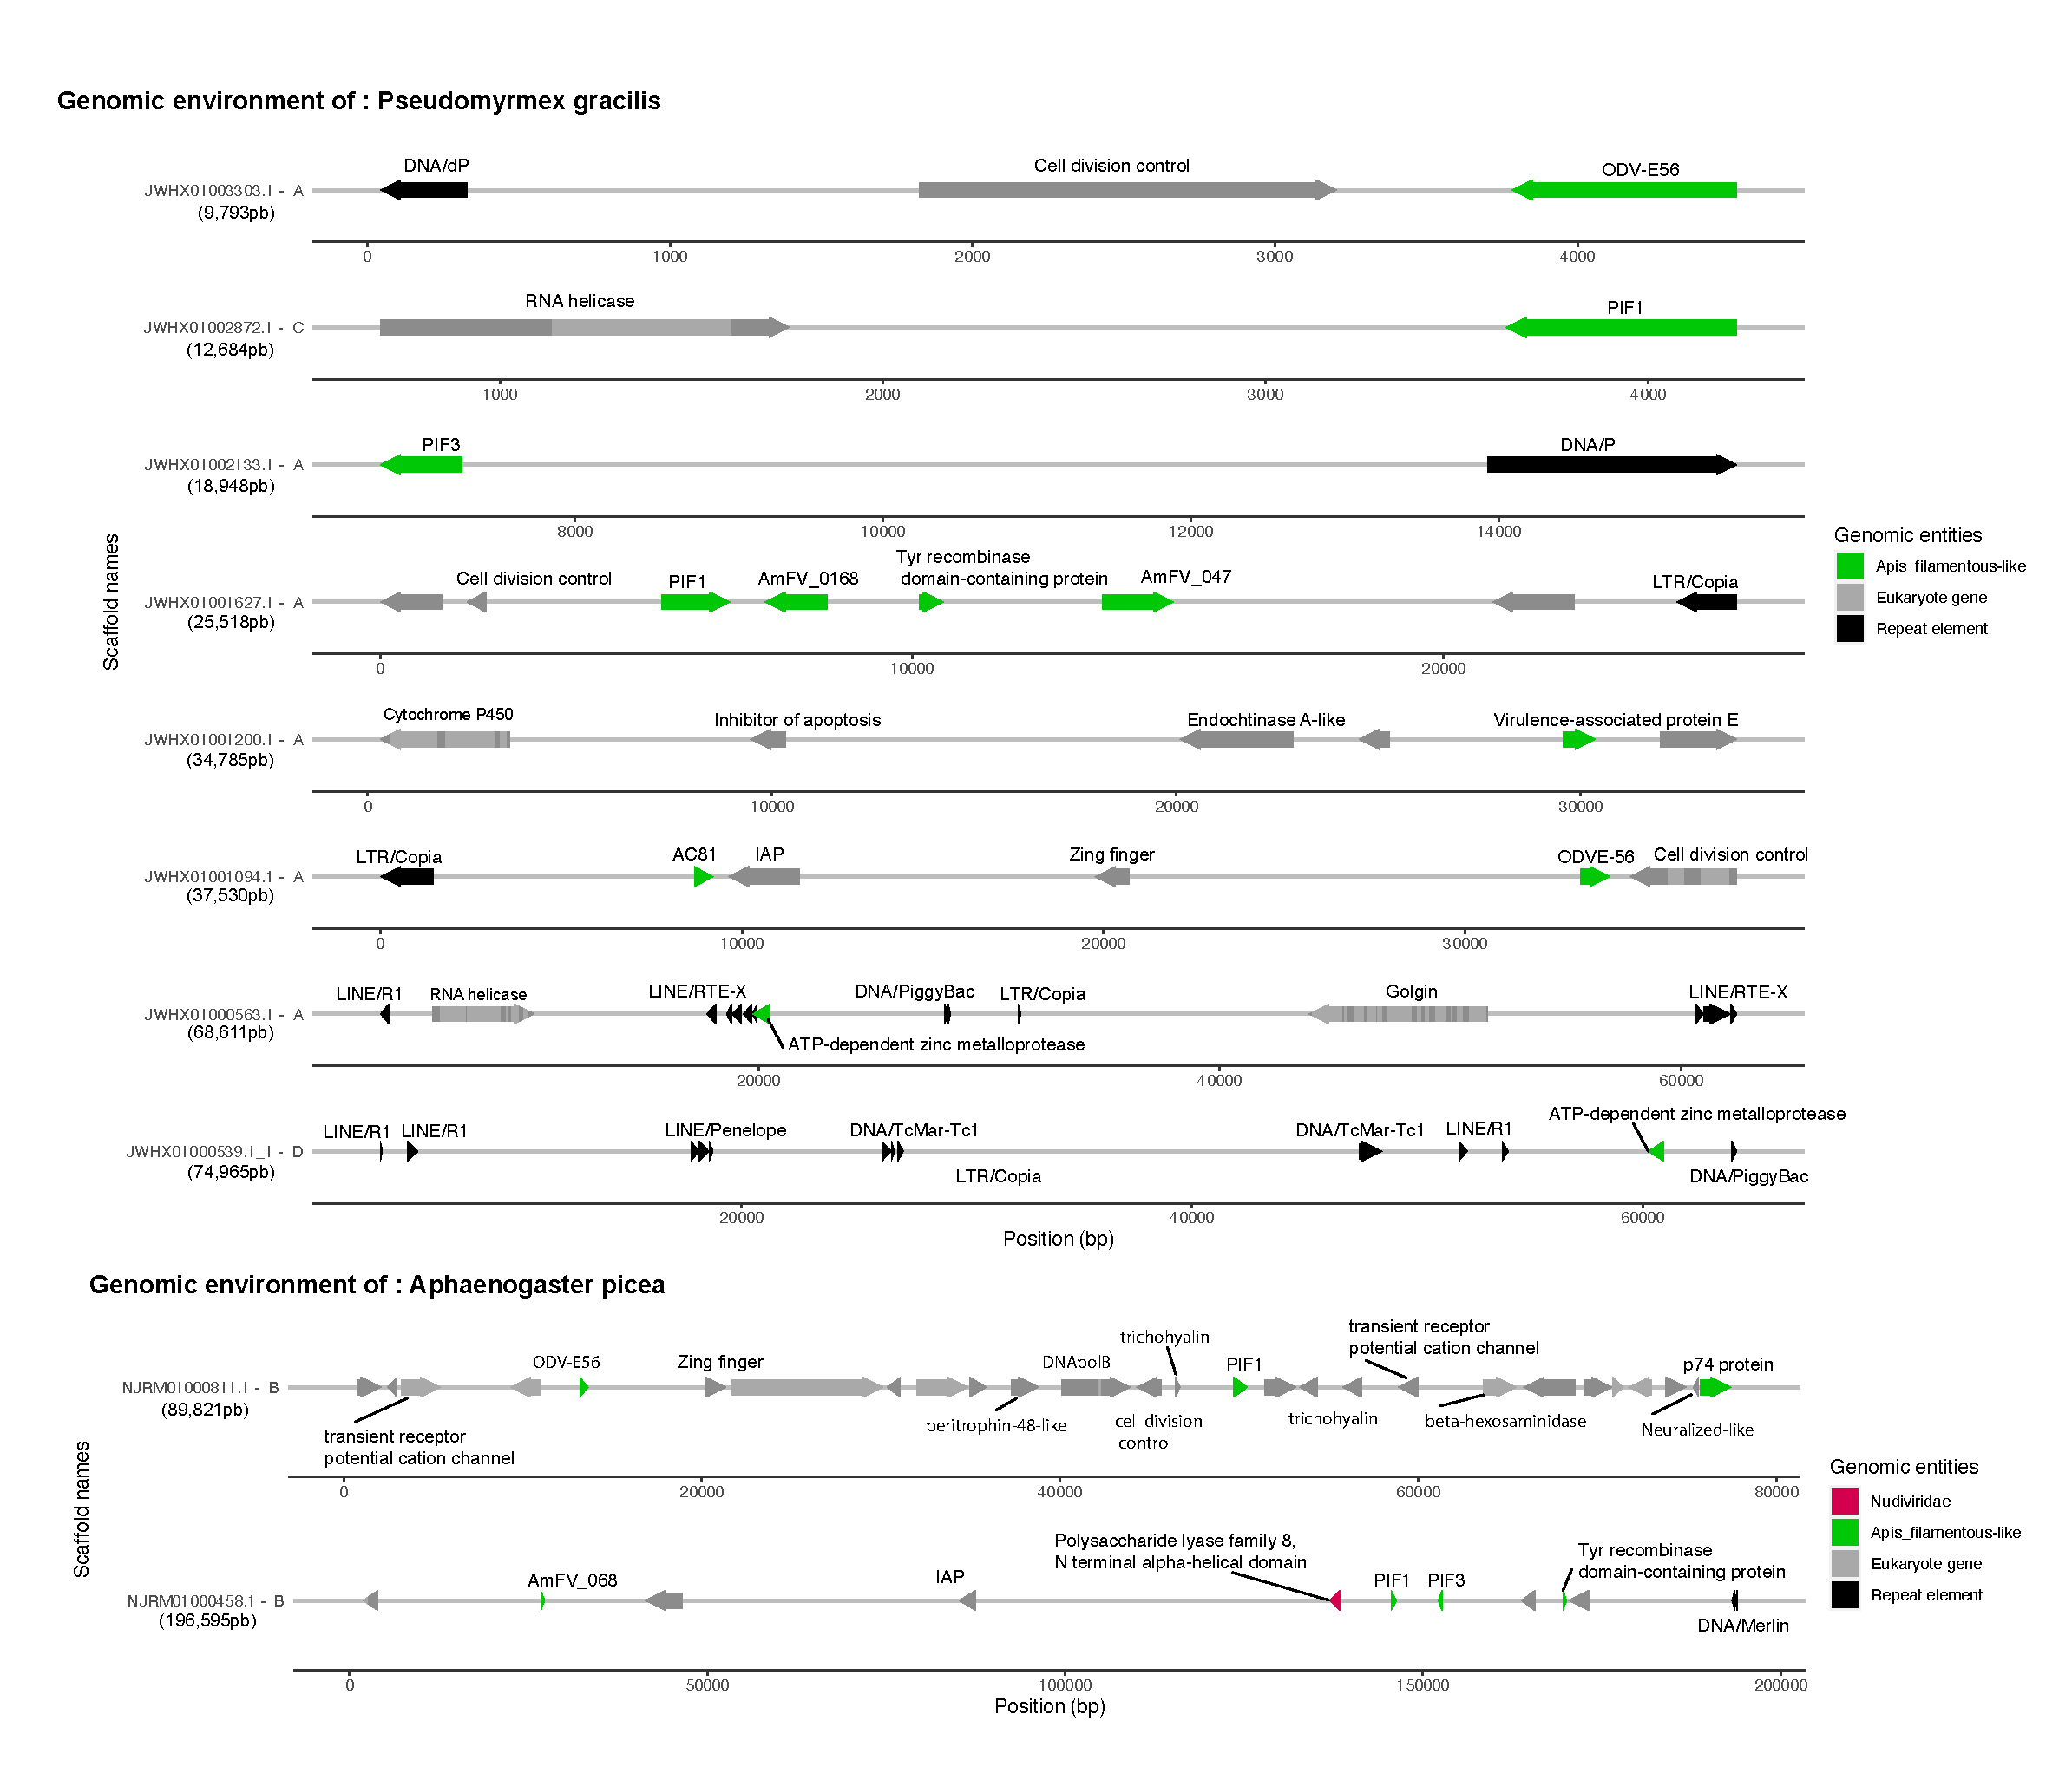
\includegraphics[width=\linewidth,height=\textheight,keepaspectratio]{PhD-master/figures/Multiple_new_integration_events_gene_plot.pdf}
\centering
\caption[Paper1:EVE distribution along scaffolds of two ant species]{\textbf{Candidate EVEs in two ant species}. In grey are displayed the eukaryotic genes predicted by Augustus, with a dark color for exons, and light for introns. In black are displayed the transposable elements predicted by sequence homologies with the RepeatPeps protein database. The size of the scaffold is displayed below the name of each scaffold. The letter followed by the scaffold name refers to the scoring given to the scaffold based on coverage and gene/ET presence information (see details in \hyperref[sec:MM-5]{Materials and methods}). For the sake of representation, all scaffolds are represented at the different scale, the exact coordinates of the elements are referred in the abscissa which corresponds to the coordinates in base pairs. Annotation is indicated above the arrows.}
\label{figure:Multiple_new_endogenization_events_gene_plot}
\end{figure}


\begin{figure}[!htpbt]
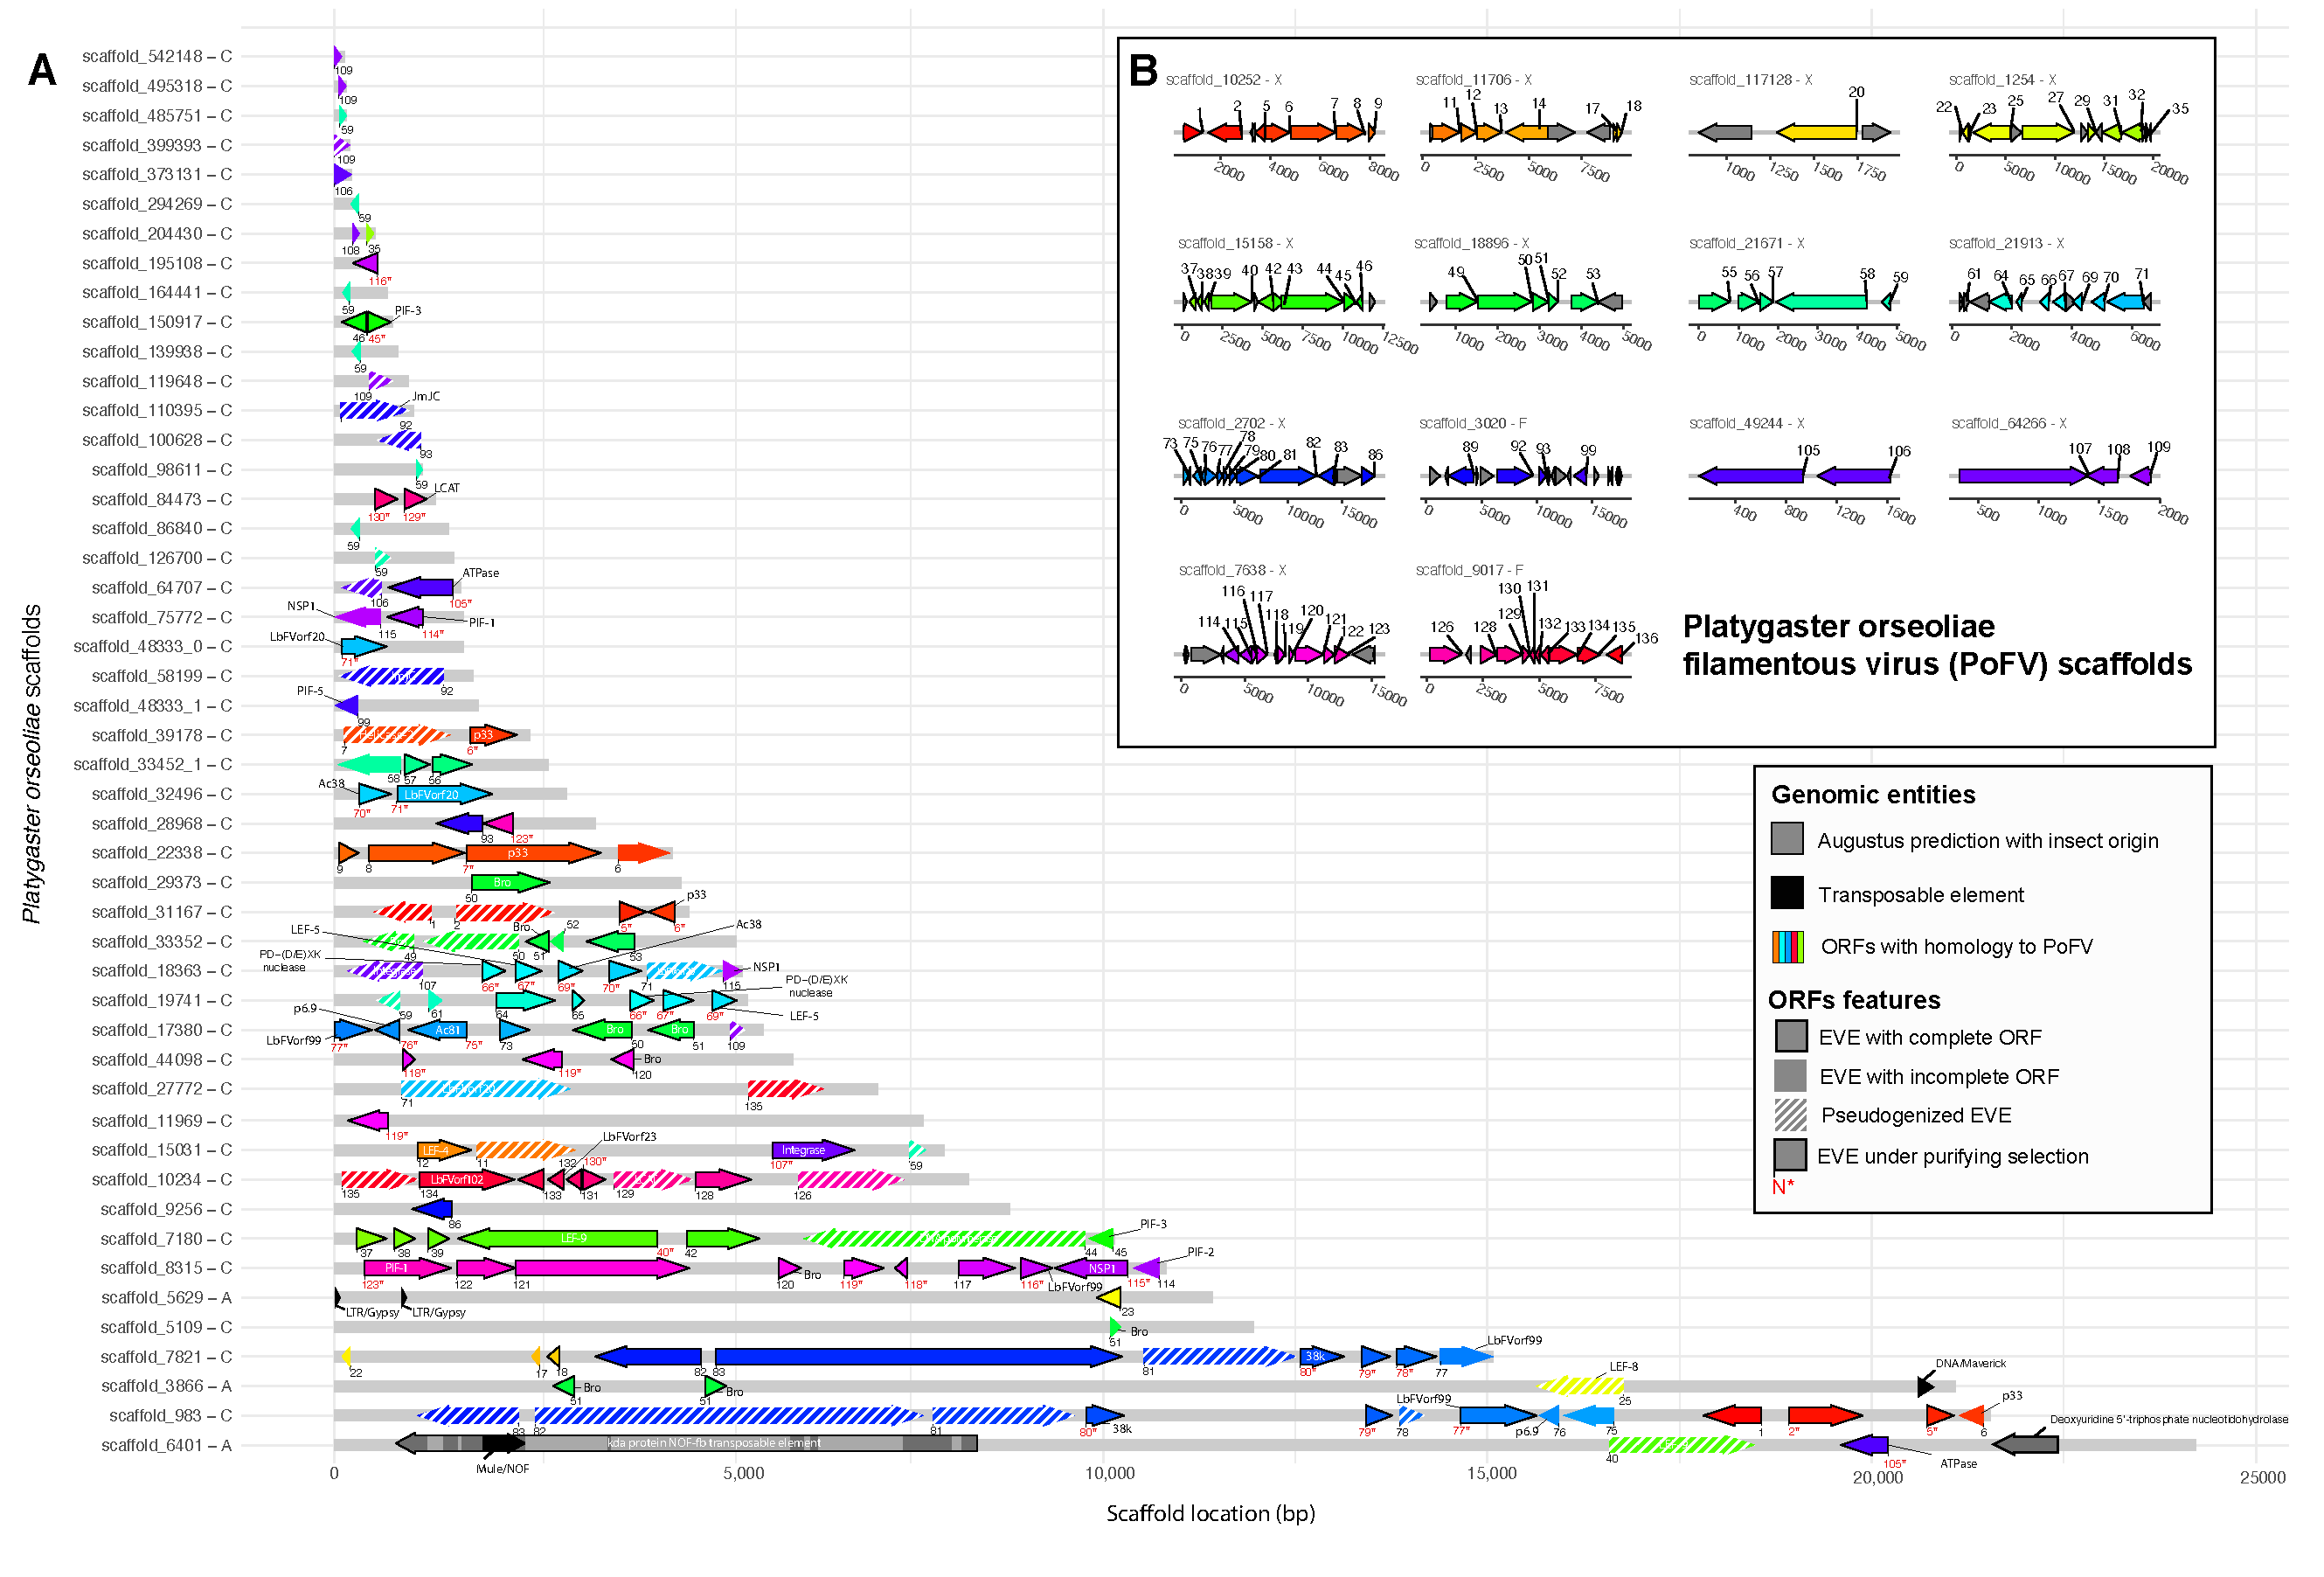
\includegraphics[width=.95\linewidth,height=.95\textheight,keepaspectratio]{PhD-master/figures/PoEFV_PoFV_table_for_GGGenes_plot.pdf}\centering
\caption[Paper1:Filamentous EVE distribution along \textit{P.orseoliae} scaffolds]{\scriptsize \textbf{Genomic environment for the EVEs detected in \textit{Platygaster orseoliae}}. The plot show regions homologous to viral ORFs in the Platygaster orseoliae filamentous virus (PoFV) genome (A). The colored regions correspond to the predicted ORFs in the PoFV genome (gray ORFS in PoFV scaffolds mean that no homologous EVEs were found in the genome of \textit{P.orseoliae}.) (B), so the closer the colours, the closer the ORFs were initially in the PoFV genome. In grey are displayed the eukaryotic genes predicted by Augustus, with a dark color for exons, and light for introns. In black are displayed the transposable elements predicted by sequence homologies with the RepeatPeps protein database (max E-value =5.866e-18). The letter followed by the scaffold name refers to the scoring given to the scaffold based on coverage and gene/ET presence information (see details in \hyperref[sec:MM-5]{Materials and methods}). The exact coordinates of the elements are referred to the x abscissa, which corresponds to the coordinates in base pairs and can be found on the GitHub file : \href{https://github.com/BenjaminGuinet/PhD_defense/blob/main/Supplementary_paper1/All_PoFV_PoEFV_loci_informations.txt}{All\_PoFV\_PoEFV\_loci\_informations.txt}. Annotation is indicated in or next to the arrows. The number below each EVE correspond to the homologous ORF number in the PoFV genome. Numbers are colored in red if the EVE has at least one paralog and if the computed \textit{dN/dS} is below 1, suggesting purifying selection in the \textit{P.orseoliae} genome. Arrow with black borders correspond to EVEs showing a complete ORF ($>$50\% of the size of the best PoFV ORF). Hatched arrows correspond to pseudogenized EVEs (with premature stop codons).   The colour difference between black and white for the names of the proteins is for visual purposes only.}
\label{figure:Porseoliae_endogenization_events_gene_plot}
\end{figure}


\begin{figure}[!ht]
 \centering
  \includegraphics[width=\linewidth,height=\textheight,keepaspectratio]{PhD-master/figures/Heatmap_control.pdf}
\caption[Paper1:Distribution of domesticated EVEs in the literature used as control]{\textbf{Heatmap representing the viral genes known to be domesticated by Hymenoptera}. 
The panel (A) refers to the four known cases (\textit{Venturia canescens}, \textit{Fopius arisanus}, \textit{Cotesia congregata} and \textit{Microplitis demolitor}) involving Nudivirus donors while the panel (B) refers to the known case involving LbFV donors in three \textit{Leptopilina} species. Complete parasitoid wasp genomes information were available for \textit{Microplitis demolitor}, \textit{Venturia canescens}, \textit{Fopius arisanus} and \textit{Cotesia congregata}, while only partial genomic data were available for \textit{Chelonus inanitus}. Each row indicates a gene which has been identified previously as being endogenized in at least one species. In (A), the first four columns indicate whether the gene is a core gene for baculoviruses (Bv), Nudiviruses (Nd), alpha-nudiviruses (alpha-Nv) or beta-nudivirus (beta-nv). The following columns indicate the presence of each gene based on the literature (in blue) and based on our pipeline (columns with a star symbol). The colors indicate the inferred selection pressure acting on each gene (\textit{dN/dS}) and the letters A, B, C, D, E, and X represent the degree of confidence in the endogenization. Capital letters indicate that this gene is present in a scaffold that contains other candidate genes. When the box is framed in black, it means that the gene is expressed (TPM$>$1000).}
\label{figure:Heatmap_control}

\end{figure}

\begin{figure}[!ht]
 \centering
  \includegraphics[width=\linewidth,height=\textheight,keepaspectratio]{PhD-master/figures/dsDNA_violin_plots_corrected_rates.pdf}
\caption[Paper1:Violin plot GLM distribution of corrected dEvent ratios]{\footnotesize\textbf{Violin plots of the posterior distribution of dEvents GLM coefficients in relation to wasp lifestyle (corrected for Events rates) }. The ectoparasitoid lifestyle is in yellow, the endoparasitoid lifestyle is in green, and the free-living lifestyle is in blue (the intercept). Coefficients have been transformed into exponential and correspond to the posterior distribution of the coefficients of a binomial logistic regression GLM model, where the lifestyle free-living stand for the intercept. The Y-axis corresponds to the multiplicative factor of the number of dEvents (corrected for Events rates) correlative to free-living species. The coefficients are derived from 1000 GLM models adjusted on 1000 randomly selected probable scenarios ($>$90 CI) of ancestral states at nodes. Branches from nodes older than 160 million years have been removed from the dataset. The ROPE\% is the percentage of the posterior distribution of coefficients below the intercept. The posterior distribution of the interaction coefficients between lifestyles and branch size were not informative, and the branch size factor was therefore added as an additive effect to the model. \textbf{A}- The corrected coefficient within all dEvents, \textbf{B}- The corrected coefficient within all dEvents without the control genomes, \textbf{C}- The corrected coefficient within all dEvents present in a scaffold annotated with a score A, \textbf{D}- The corrected coefficient within all dEvents present in a scaffold annotated with a score A and without the control genomes.}
\label{figure:dsDNA_violin_plots_corrected_rates}
\end{figure}


\begin{figure}[!ht]
 \centering
  \includegraphics[width=\linewidth,height=\textheight,keepaspectratio]{PhD-master/figures/Campopleginae_synteny.pdf}
\caption[Paper1:IVSPER gene distribution along Campopleginae scaffolds]{ \textbf{IVSPER genes identified in the Campopleginae genome}. The figure compares the synteny of the IVSPER between Hyposoter didymator ichnovirus (HdIV) and  the Campoplegninae of our dataset. Homologous genes with
synteny between the two species are indicated by grey shading. The direction of the arrows corresponds to the sense and anti-sense strand. The color of the boxes is unique to each IVSPER. }
\label{figure:Campoplegniae_synteny}
\end{figure}

\begin{figure}[!ht]
 \centering
  \includegraphics[width=\linewidth,height=\textheight,keepaspectratio]{PhD-master/figures/Ophioniformes_phylogeny.pdf}
\caption[Paper1:Recapitulation of Ichnovirus within Ophioniformes wasps]{\textbf{Cladogram of the Ophioniformes group, illustrating the two independent endogenization events of two unknown viruses in Banchinae and Campopleginae lineages}. The phylogeny includes 12 subfamilies of the Ophioniformes group within the superfamily \textitit{Ichneumonoidea}. Several species of these subfamilies have been examined for the presence of ichnovirus-like polydnaviruses: by negative staining of calyx fluid (N), TEM of ovarian sections (S), visual examination of the calyx fluid (CF), probes from ichnovirus replication or structural proteins (probes) or by IVSPER sequence homology on whole genome assemblies (WG). The subfamilies and species in blue correspond to those positive for a dsDNA virus endogenization from unknown origin (ichnovirus-like). The others (in black) were negative for endogenized ichnovirus-like elements.
The phylogeny is inspired from \cite{sharanowski_phylogenomics_2021},  and the data reported comes from \cite{sharanowski_phylogenomics_2021,beliveau_genomic_2015,cusson_genomics_2012, legeai_genomic_2020}.}.
\label{figure:Ophioniformes_phylogeny}
\end{figure}

\begin{figure}[!ht]
 \centering
  \includegraphics[width=\linewidth,height=\textheight,keepaspectratio]{PhD-master/figures/Bioinformatic_pipeline.pdf}
\caption[Paper1:Simplified summary of the bioinformatics pipeline for the detection of EVEs and dEVEs]{Simplified summary of the bioinformatics pipeline for the detection and validation of candidates for endogenization
and domestication.}
\label{figure:Bioinformatic_pipeline}
\end{figure}

\begin{figure}[!htpb]
 \centering
  \includegraphics[width=\linewidth,height=\textheight,keepaspectratio]{PhD-master/figures/Event_assignation_examples.pdf}
\caption[Paper1:Canonical examples of endogenization events]{\textbf{Canonical examples of endogenization events inferred by our pipeline}. 
The column "Sp names" contains the species name, followed by the name of the scaffold in which the EVE has been identified. The "Viral family" column refers to the putative viral family that donated the EVEs. The column "Cluster number" corresponds to the number of the corresponding cluster phylogeny (thus the EVE phylogeny). The "Monophyletic clade number" column corresponds to the number of the monophyletic clade within a cluster (can be a single locus or  multiple loci). The column "Event number" is the number given to single/multiple EVEs that derive from the same endogenization event.}
\label{figure:Event_assignation_examples}
\end{figure}


%\section{Article}

%\includepdf[pages=-,pagecommand={}]{PhD-master/PDF_files/papier-108.pdf}


    \thispagestyle{empty}
    \chapter{Proposal for a new \textit{\textit{Naldaviricetes}} viral family associated with Hymenoptera parasitoids}
    \label{chap:LbFV-Family-description}
    
        \begin{center}
        \Large Benjamin Guinet$^{\text{1}}$$^{\text{*}}$, Matthieu Leobold$^{\text{2}}$$^{\text{*}}$, Nelly Burlet$^{\text{1}}$, Jean-Michel Drezen$^{\text{2}}$, Elisabeth Herniou$^{\text{2}}$, Annie Bézier$^{\text{2}}$$^{\text{*}}$, Julien Varaldi$^{\text{1}}$$^{\text{*}}$\\
        \vspace{0.5cm}
        \normalsize
        $^{\text{1}}${Université Lyon 1, CNRS, Laboratoire de Biométrie et Biologie Evolutive UMR 5558, F-69622 Villeurbanne, France.}\\
        $^{\text{2}}${Institut de recherche sur la biologie de l'insecte UMR7261 Université de Tours, Centre National de la Recherche Scientifique : UMR7261 Av Monge 37200 Tours, France.}\\
        $^{\text{*}}${Co-first and co-last authors.}\\
    \end{center}
     \setcounter{minitocdepth}{1}

    {\hypersetup{linkcolor=GREYDARK}\minitoc}

\clearpage

\label{sec:chap2}

\section{Reproducibility and Supplemental material}

All supplementary material named with a "GitHub" mark, can be found within the following GitHub repository : \href{https://github.com/BenjaminGuinet/PhD_defense/tree/main/Supplementary_paper2}{Supplementary\_paper2}. An e-mail authorization must have been sent to all members of the jury.

\section{Abstract}

Large dsDNA viruses from the \textit{Naldaviricetes} class are currently composed of four viral families infecting insects and/or crustaceans. Since the 1970s, particles described as filamentous viruses have been observed by electronic microscopy in several species of Hymenoptera parasitoids but until recently no genomic data was available. This study provides the first comparative genomic analyses of these filamentous viruses. We studied the genomes of seven filamentous viruses, six of which were newly obtained, in addition to the previously sequenced Leptopilina boulardi filamentous virus (LbFV), to gain a better understanding of their evolutionary history. We show that filamentous viruses related to LbFV share morphological, genomic and phylogenetic features that distinguish them from their closest relatives, i.e. \textit{Hytrosaviridae}. Additionally, these filamentous viruses share all genomic features of the \textit{Naldaviricetes} but their core genome comprises five specific genes that clearly distinguish them from Hytrosaviruses. Furthermore, by mining public databases, we provide evidence suggesting they preferentially infect Hymenoptera with parasitoid lifestyle. Finally, we propose a taxonomical revision of the class \textit{Naldaviricetes} in which filamentous viruses related to LbFV constitute a fifth family within the order \textit{Lefavirales}. We propose to name this new family, Filamentoviridae. 

\section{Introduction}

All cellular life forms are associated with viruses \citep{kristensen_new_2010,koonin_virocentric_2013}. However, rough but reasonable estimations of viral diversity suggest that only 1\% of all eukaryotic viruses has been discovered and classified \citep{geoghegan_comparative_2017}. Because arthropods are the most diverse taxonomic group of animals, we may expect that a great fraction of this unknown viral diversity is hosted by arthropods. Indeed, our assessment of arthropod viral diversity has recently been progressing thanks to the development of high-throughput sequencing technologies. These technologies permitted deep (possibly meta-) genomic and transcriptomic analysis that uncovered part of this unknown diversity \citep{ dolja_metagenomics_2018,roux_diversity_2022, wu_abundant_2020,schulz_giant_2020}. For RNA viruses, the discovery of new lineages is facilitated by presence of the universal RNA-dependent-RNA polymerase. By screening RNAseq datasets, it has been possible to identify tens or thousands of new viruses in single large-scale bioinformatic analysis \citep{shi_evolutionary_2018, wu_abundant_2020, medd_virome_2018,obbard_new_2020}. On the contrary, DNA viruses do not share any universal genes \citep{koonin_global_2020} and are prone to extensive gene loss, gain, and exchange. These features thus make exploration of the "DNA virosphere" more challenging.  

Among eukaryotic large dsDNA viruses, the \textit{Naldaviricetes} forms a monophyletic class of arthropod-infecting viruses with specific features. These viruses have circular genomes replicating in the nucleus and packaged into enveloped rod-shaped nucleocapsids. They belong to four families: the \textit{Baculoviridae}, \textit{Nudiviridae}, \textit{Hytrosaviridae}, and \textit{Nimaviridae} \citep{harrison_ictv_2020}. They share a group of genes that encode the so-called \textit{per os} infectivity factors (PIFs). PIFs are required for baculovirus entry into midgut goblet cells during primary infection (Rohrmann, 2019) and they may be involved in particle entry into other cell types, i.e., salivary glands for hytrosaviruses \citep{abd-alla_genome_2008,garcia-maruniak_sequence_2008}, gonad cells for Helicoverpa zea nudivirus 2 \citep{hamm_oviposition_1996,burand_analysis_2012} and all cell types of the parasitized Lepidoptera for bracoviruses (endogenous nudiviruses found in some parasitic wasps) \citep{bezier_polydnaviruses_2009, muller_genome-wide_2021}. Among \textit{Naldaviricetes}, the \textit{Baculoviridae}, the \textit{Nudiviridae}, and the \textit{Hytrosaviridae} form the order \textit{Lefavirales}. This name derives from the fact that they share the so-called \textit{lef} genes (for late expression factor) encoding the different subunits of a specific viral \textit{RNA polymerase}. These \textit{lef} genes ensure transcription of viral genes in the late phase of infection. 

Since the 1970s, investigations using electron microscopy uncovered a variety of viruses in the reproductive tract of Hymenopteran parasitic wasps. In particular, several endoparasitoid wasp species were found to harbor long flexible rod-shaped enveloped particles replicating in their ovaries. These particles are often secreted in the genital fluid, which is injected during wasp oviposition into the parasitized host. Because of the peculiar shape of these particles, the viruses were referred to as "filamentous viruses" (FVs). Such FVs were described in different species: a Campopleginae (\textit{Diadegma terebrans}), a series of Braconidae (\textit{Cotesia congregata}, \textit{Cotesia hyphantriae}, \textit{Cotesia marginiventris}, \textit{Microplitis croceipes} and \textit{Microplitis rufiventris}) and a Figitidae (\textit{Leptopilina boulardi}) \citep{krell_replication_1987, de_buron_characterization_1992,  stoltz_viruses_1979, hamm_comparative_1990,hegazi_calyx_2005, varaldi_infectious_2003,varaldi_artifical_2006}.

More recently, a first "filamentous virus" was characterized at the molecular level from the \textit{Drosophila} parasitoid \textit{Leptopilina boulardi} \citep{lepetit_genome_2017}. This virus was named Leptopilina boulardi filamentous virus (LbFV) and phylogenetic analysis clearly identified it as a sister group of hytrosaviruses, known to induce salivary gland hypertrophy symptoms in dipteran adults \citep{abd-alla_hytrosaviridae_2009}. However, it has been suggested that this virus may belong to a new family based on its high sequence divergence from \textit{Hytrosaviridae} \citep{lepetit_genome_2017}. Interestingly, LbFV has a strong impact on the wasp egg-laying behavior: infected females readily accept to lay their eggs in already parasitized hosts, contrary to uninfected ones \citep{varaldi_infectious_2003,varaldi_artifical_2006}. This induction of "superparasitism" permits virus horizontal transmission, thus increasing its fitness at the expense of wasp fitness \citep{gandon_superparasitism_2006}. Furthermore, an ancestral integration of a related virus has been described in \textit{Leptopilina} species (Di Giovanni et al., 2020). Similarly to other parasitoid wasp species that have domesticated viruses \citep{bezier_polydnaviruses_2009,volkoff_analysis_2010,pichon_recurrent_2015, burke_common_2019}, these endogenized viral genes have been domesticated and are employed by female wasps as a means of delivering virulence factors, which are necessary to protect their eggs from the host immune system \citep{rizki_parasitoid_1990, di_giovanni_behavior-manipulating_2020}. Recently, sequences of a virus related to LbFV were detected in a sample of field-collected \textit{Drosophila melanogaster} (DmFV) \citep{wallace_discovery_2021}. Given the potential high prevalence of \textit{Leptopilina} parasitoids in the field \citep{patot_prevalence_2010}, it is unclear whether this virus was really infecting \textit{Drosophila} cells or whether it was introduced into the \textit{Drosophila} by an infected parasitic wasp during an unsuccessful parasitization event. Another type of distantly related filamentous virus is known to infect \textit{Apis mellifera} (AmFV). Also belonging to the \textit{Naldaviricetes}, this virus however lacks genomic characteristics from the \textit{Lefavirales} \citep{gauthier_apis_2015, yang_genomics_2022}. 

In this study, we characterize six new virus genomes related to LbFV, infecting wasps that belong to three Hymenoptera superfamilies (Cynipoidea, Chalcidoidea and Ichneumonoidea). By in-depth comparative genomic and phylogenomics of their genomes together with particle morphogenesis comparison, we explore the possibility that these "filamentous viruses" constitute a new viral family within \textit{Naldaviricetes}. We show that these filamentous viruses share morphological, genomic and phylogenetic features that distinguish them from their closest relatives, i.e. \textit{Hytrosaviridae}. Additionally, by mining public databases, we provide evidence suggesting that filamentous viruses preferentialy infect Hymenoptera with parasitoid lifestyle.  We therefore propose a taxonomical revision of the class \textit{Naldaviricetes} in which filamentous viruses related to LbFV do not belong to \textit{Hytrosaviridae} but constitute a fifth family within the order \textit{Lefavirales}. We propose to name this new family Filamentoviridae. 

\section{Results}

\subsection{Genomes of filamentous viruses related to LbFV have similar structures}   

We analyzed the genome sequence of six novel viruses related to the Leptopilina boulardi filamentous virus (LbFV). All of them were obtained from parasitoid wasps, namely \textit{Leptopilina heterotoma} (Cynipoidea, Figitidae), \textit{Encarsia formosa} (Chalcidoidea, Aphelinidae), \textit{Platygaster orseoliae} (Platygastroidea, Platygastridae), \textit{Psyttalia concolor} (Ichneumonoidea, Braconidae) and two \textit{Cotesia congregata} incipient species (Ichneumonoidea, Braconidae). One viral sequence was retrieved following particle purification while the other five were discovered after genome sequencing of parasitoid wasps (\figurename{\ref{figure:Table_genomes_filamentous}}). In the following, the viruses are referred to as the two initials of the binomial latin name of the wasp followed by FV for filamentous virus (i.e.: LhFV, EfFV, PoFV, PcFV, CcFV1 and CcFV2, respectively).  

In the five datasets obtained from parasitoid whole genome sequencing projects, we had to ensure that the putative viral contigs were not endogenized in wasp chromosomes. To do so, we studied the sequencing depth or coverage for each contig. Our expectation was that the coverage should differ between wasp chromosomes and viral chromosomes, since the probability that both entities had the same density in the DNA extract is most likely low. As expected, coverage was significantly different between viral and parasitoid contigs for all five biological models (\figurename{\ref{figure:ALL_filamentous_cov_GC_plot}}), strongly suggesting that viral contigs effectively belong to exogenous viruses. The minimal coverage for the presumably viral contigs was high for four of them (\figurename{\ref{figure:ALL_filamentous_cov_GC_plot}}). The last genome (EfFV) had only an approximate 24x coverage based on short reads. However, the additional long read sequencing that was performed on this genome led to a single circular molecule (\figurename{\ref{figure:CcFV1_CcFV2_EfFV_circos}}), confirming that this was indeed a viral genome. Two other genomes (CcFV1 and CcFV2) were also obtained after long-read or Illumina paired-end sequencing (\figurename{\ref{figure:Table_genomes_filamentous}}), leading to a single circular DNA molecule, strongly suggesting that they were complete (\figurename{\ref{figure:CcFV1_CcFV2_EfFV_circos}}). Even though no circular forms could be obtained for the three other genomes (LhFV, PoFV and PcFV), we consider that the obtained sequences are nearly complete since contig cumulative sizes range from approx 106 to 131 kb which is comparable to those of the four circularized FV genomes: approx 111 kb (LbFV), approx 101 kb (CcFV1), approx 138 kb (CcFV2) and 164 kb (EfFV) (\figurename{\ref{figure:Table_genomes_filamentous}}); and more globally to other \textit{Lefavirales} genomes (\textit{Baculoviridae}: 80-180 kb, \textit{Nudiviridae}: 97-232 kb and \textit{Hytrosaviridae}: 125-191 kb) (GitHub:\href{https://github.com/BenjaminGuinet/PhD_defense/blob/main/Supplementary_paper2/Table%20S2.xlsx}{TabS2}). Of note, LhFV sequences have 97.98\% nucleotidic identity with the recently published sequences annotated as Drosophila-associated filamentous virus (DmFV). Such contigs were indeed detected after mining genomic sequences obtained from 6668 pool-sequenced \textit{Drosophila}, sampled from forty-seven European locations \citep{wallace_discovery_2021}. Among these samples, one single was positive for DmFV. Thus, adding to our results the fact \textit{Leptopilina} species (e.g., \textit{L. boulardi} and \textit{L. heterotoma}) parasitize \textit{Drosophila} larvae \citep{kopelman_immature_1984,schlenke_contrasting_2007}, the authors acknowledged they could not detect any DmFV sequences in \textit{D. melanogaster} public datasets and the virus they sequenced could infect the parasitoid wasp rather than the fly \citep{wallace_discovery_2021}; it is likely that LhFV and DmFV correspond to one single virus infecting a wasp that had previouly parasitized the sequenced \textit{Drosophila}.  

Additionally, de novo gene prediction showed a composition of 110 to 128 ORFs for these three non-circularized genomes, which is comparable to the number of ORFs predicted for the three new circular genomes (CcFV1 = 104, CcFV2 = 112, and EfFV = 156; (\figurename{\ref{figure:Table_genomes_filamentous}}, and GitHub:\href{https://github.com/BenjaminGuinet/PhD_defense/blob/main/Supplementary_paper2/Table%20S3.xlsx}{TabS3}), and more generally to related viruses (LbFV = 108, \textit{Naldaviricetes} = 90-241). The presence of repetitive sequences as previously observed for LbFV \citep{lepetit_genome_2017}, is probably the reason underlying our incapacity to circularize these three genomes using short reads only (\figurename{\ref{figure:Table_genomes_filamentous}}). Finally, all six virus genomes had high gene densities (min = 79.9\% and max = 92\%) as observed for viruses belonging to \textit{Naldaviricetes} (\figurename{\ref{figure:Table_genomes_filamentous}}). Altogether, these data strongly suggest that the six novel viral sequences presented here represent complete circularized or complete non-circularized viral genomes.  

\subsection{The filamentous virus core gene set} 

Viral genomes contain two types of genes. On the one hand, the core genes are defined as the set of genes shared by all members of a virus family and are generally involved in essential functions in the virus cycle. On the other hand, accessory genes may be specific to a clade or to particular viruses, may be involved in adaptation to the host, and sometimes acquired from infected hosts by horizontal gene transfer. Only core genes are relevant for the phylogenetic inference of the virus relationships within the virosphere. 

The analysis of the seven filamentous viruses, excluding the contigs of DmFV \citep{wallace_discovery_2021}, resulted in the identification of a set of 29 core genes (\figurename{\ref{figure:dsDNA_filamentous_heatmap}} and GitHub:\href{https://github.com/BenjaminGuinet/PhD_defense/blob/main/Supplementary_paper2/Table%20S4.xlsx}{TabS4}). About two thirds of the genes are homologs of core genes found in different \textit{Lefavirales} and are involved in specific viral transcription, packaging of the virus DNA in the nucleocapsids, assembly and morphogenesis of the particles or virus entry into infected cells (infectivity) as characterized mainly in baculoviruses (\figurename{\ref{figure:dsDNA_filamentous_heatmap}}, green columns). Eight conserved genes encode proteins with unknown function as no sequence similarity was detected (\figurename{\ref{figure:dsDNA_filamentous_heatmap}}). Among these genes, five were strictly specific to FVs related to LbFV (\figurename{\ref{figure:dsDNA_filamentous_heatmap}}, blue columns). 

 \begin{figure}[!htpbt]
\includegraphics[width=\linewidth,height=\textheight,keepaspectratio]{PhD-master/figures/dsDNA_filamentous_heatmap.pdf}\centering
\caption[Paper2:\textit{Naldaviricetes} core genes heatmap]{\textbf{Heatmap representing the core gene content of LbFV related FVs (LbFV-like) compared to other \textit{Naldaviricetes} dsDNA viral species}. A cladogram phylogeny is reported on the right. The rows represent the viral species, and the columns represent the genes distributed according to their potential functions. Colored cells represent the presence of the gene in viral genomes (pale yellow = core genes shared by \textit{Naldaviricetes} species, green = core genes shared by \textit{Lefavirales} species, red = FV and hytrosavirus core genes, blue = FV core genes and grey = presence in other virus genomes).}
\label{figure:dsDNA_filamentous_heatmap}
\end{figure}

In the section that follows, we will first provide evidence that filamentous viruses related to LbFV (i.e., Filamentoviridae) possess all the necessary genes to be classified as \textit{Naldaviricetes} as well as \textit{Lefavirales} clades. We will then provide information regarding the putative function of some of these filamentous core genes. 

All the core genes shared by the \textit{Naldaviricetes} including the per os infectivity factors (\textit{p74}, \textit{pif-1}, \textit{pif-2}, \textit{pif-3} and \textit{pif-5}), the \textit{DNA polymerase} (\textit{DNApol}) and the sulfhydryloxidase (\textit{p33}) were present in the analyzed FV genomes (\figurename{\ref{figure:dsDNA_filamentous_heatmap}}, pale yellow columns). Five out of the six known \textit{Lefavirales} core genes can also be unambiguously predicted as functional ORFs within these genomes, including three subunits of the RNA polymerase (\textit{lef-4}, \textit{lef-8} and \textit{lef-9}), the helicase (nudiviral \textit{helicase 2} homolog) and the \textit{Ac81} genes (\figurename{\ref{figure:dsDNA_filamentous_heatmap}}, green columns). In addition, a complete \textit{lef-5} ORF (the fourth subunits of the \textit{Lefavirale} RNA polymerase) was identified in CcFV1, CcFV2, EfFV, PcFV and PoFV genomes, but could be predicted using alternative start codons in LbFV, LhFV and DmFV genomes. Consistent with the hypothesis that this gene is functional in LbFV, RNAseq mapping of reads from \textit{L. boulardi} head and abdomen \citep{varaldi_deciphering_2018} indicated that this ORF is indeed fully transcribed (median coverage = 256X where the highest expressed (ORF89) displayed a median of 7428X). Furthermore, we identified genes encoding for two potential nucleocapsid proteins (\textit{38k} and \textit{P6.9}) for which no homologs had previously been reported in hytrosavirus genomes, despite being present in all \textit{Baculoviridae} and \textit{Nudiviridae}. However, a thorough search using HMMER tool allowed us to identify that MdSGHV073 from MdSGHV (YP\_001883401.1, e-value: 0.000095) and SGHV044 from GpSGHV-Uga (YP\_001686992.1) corresponded to hytrosavirus \textit{38k} homologs, which makes the nucleocapsid \textit{38k} an additional seventh core gene shared by all \textit{Lefavirales} (\figurename{\ref{figure:dsDNA_filamentous_heatmap}}, green columns).  The corresponding products have been characterized as virion (GpSGHV-Uga, \citep{kariithi_proteomic_2010}) and nucleocapsid components (GpSGHV-Eth, AMB48649.1; \citep{abd-alla_comprehensive_2016}), like in baculoviruses \citep{blissard_baculovirus_2018}. Likewise, we identified MdSGHV026 (YP\_001883354.1) as a potential hytrosavirus \textit{P6.9} homolog, but we were not able to find a homolog in GpSGHV genomes. This makes thus \textit{P6.9} a first FV-specific core gene compared to hytrosaviruses (\figurename{\ref{figure:dsDNA_filamentous_heatmap}}, blue columns).  

Of the remaining FV-core genes with known or predicted functions, four (\textit{integrase}, lecithin:cholesterol acyltransferase (\textit{lcat}), \textit{ATPase/CD48} and \textit{PD-(D/E)XK nuclease}) have homologs in all hytrosavirus genomes (\figurename{\ref{figure:dsDNA_filamentous_heatmap}}, in red).  Except for \textit{lcat}, their homolog in GpSGHV-Eth encode virion, nucleocapsid or envelope components \citep{abd-alla_comprehensive_2016}. In contrast, a fifth gene, \textit{Ac38}, is found in a single species (GpSGHV), which makes it also a second FV-specific core gene compared to hytrosaviruses (\figurename{\ref{figure:dsDNA_filamentous_heatmap}}, blue columns). \\

\textit{Ac38} homologs have been reported in all lepidopteran baculoviruses (Alpha- and Betabaculovirus) where they are associated with budded virus envelopes \citep{wang_characterization_2005}. Their products contain a conserved Nudix motif (nucleoside diphosphate X, \citep{mildvan_structures_2005}), which is suspected to negatively regulate viral gene expression by acting as a decapping enzyme in vaccinia virus \citep{parrish_characterization_2007}.\\ 

\textit{Integrase} homologs are nudivirus and bracovirus, but not baculovirus, core genes \citep{petersen_naked_2022}. In Bracoviruses, the corresponding product is involved in the provirus DNA excision \citep{burke_mutualistic_2013}) and is one of the viral particle components \citep{burke_widespread_2014}. \\

\textit{Lecithin:cholesterol acyltransferases} are catabolic enzymes usually involved in the lipid metabolic process, that are activated by apolipoproteins \citep{saeedi_review_2015}. Although proteins with \textit{LCAT} \citep{garcia-maruniak_sequence_2008, lepetit_genome_2017, wallace_discovery_2021} or apolipoprotein domains \citep{gauthier_apis_2015, lepetit_genome_2017} were identified in several dsDNA viruses infecting insects, their role in virus cycle has not yet been documented. Interestingly, in the protozoan parasite \textit{Toxoplasma gondii}, a \textit{LCAT} protein was shown to facilitate parasite cytolytic egress from infected cells \citep{pszenny_lipolytic_2016}, a function that could also be shared by the viral \textit{LCAT}. \\

\textit{PD-(D/E)XK nuclease} (pfam12705) homologs are found in prokaryotes, in giant viruses but also in a betabaculovirus (Diatraea saccharalis granulovirus, \citep{ardisson-araujo_betabaculovirus_2016}) and in AmFV \citep{gauthier_apis_2015}. The biological functions of these enzymes are unknown; however, they could be involved in DNA replication or processing \citep{steczkiewicz_sequence_2012}.\\ 

As for the \textit{ATPases} from the AAA+ superfamily, they were identified in all organisms where they participate in diverse cellular processes including membrane fusion, proteolysis, DNA recombination, replication and repair but also viral replication \citep{ogura_aaa_2001, snider_aaa_2008,khan_oxidative_2022}. Hytrosavirus homologs further display similarity with cell division control protein 48 and/or vacuolar protein sorting-associated protein which suggest that these proteins may also have a role in virus morphogenesis and egress \citep{kolesnikova_vacuolar_2009, hilbert_structure_2015,ahmed_crystal_2019,huttunen_vaccinia_2021}.\\

Finally, a HHpred analysis \citep{gabler_protein_2020} based on LbFV\_ORF92 homologous sequence alignment (either for FVs or for hytrosaviruses, alone) points to viral primase, \textit{helicase}, ssDNA-binding protein candidates (up to 98.66\% probability from positions 1,358 to 1,503 and 97.57\% probability from positions 1,487 to 1,613, respectively). Such a function assignment could make them the homologs of the baculovirus \textit{lef-3} gene product \citep{evans_characterization_1999} as suggested for the FV homolog from \textit{Dolichomitus sp} (MBT0716627.1) and the hytrosavirus homologs infecting \textit{Glossina} (AMB48650.1) or \textit{Drosophila} (QXE96913.1). However, these proteins are very different in size between the baculovirus \textit{lef-3} (approx 390 aa), the  hytrosavirus proteins (approx 1,750 aa) and those from FVs (from 1,593 to 2,145 aa) and the similarities are weak, therefore we preferred to keep the name of LbFV\_ORF92, rather than making a wrong assignment, while still placing it in the DNA replication/processing section as suggested by the HHpred analysis. Their GpSGHV-Eth homolog has been reported to be an envelope component \citep{abd-alla_comprehensive_2016}.\\

Concerning the eight FV core genes for which no function could be inferred, three (LbFV\_orf5, LbFV\_orf20 and LbFV\_orf102) display sequence homology in both hytrosaviruses (\figurename{\ref{figure:dsDNA_filamentous_heatmap}}, red columns). Their corresponding homologs were shown to be part of the nucleocapsid or the tegument compartments in GpSGHV-Eth \citep{abd-alla_comprehensive_2016}. Ultimately, we found that five genes (LbFV\_orf23, LbFV\_orf54, LbFV\_orf87, LbFV\_orf94 and LbFV\_orf99) were specific of FVs, which brings to seven the number of FV-specific core genes compared to hytrosaviruses, when adding \textit{Ac38} and \textit{P6.9} (\figurename{\ref{figure:dsDNA_filamentous_heatmap}}, blue columns). 

\subsection{Update on the phylogeny of the \textit{Naldaviricetes}} 

To determine the relationships between the eight available FVs within the \textit{Naldaviricetes} (Github:\href{https://github.com/BenjaminGuinet/PhD_defense/blob/main/Supplementary_paper2/Table%20S2.xlsx}{TabS4}), two phylogenetic approaches were undertaken. The first is a rather classical inference based on the protein predicted from the 29 FV core genes (Github:\href{https://github.com/BenjaminGuinet/PhD_defense/blob/main/Supplementary_paper2/Table%20S4.xlsx}{TabS4}) using both Bayesian and Maximum Likelihood estimation models, and the second, referred to an "all genes" approach, is a phylogenomic approach taking into account all the proteins encoded by at least four viral species. The datasets encompass alignments of 7,031 sites for the "core genes" approach and 17,114 sites for the "all genes" approach. 

First, all phylogenetic analyses resulted in very similar tree topologies, and revealed that the FVs formed a highly supported monophyletic clade, sister group to the \textit{Hytrosaviridae} (\figurename{\ref{figure:dsDNA_phylogeny_filamentous}}, \figurename{\ref{figure:Bayesian_vs_ML_cophylogeny_filamentous}}). An uncertainty in the phylogenies was on AmFV positioning, which was either placed at the base of the \textit{Lefavirales} clade (\figurename{\ref{figure:dsDNA_phylogeny_filamentous}}), or the \textit{Hytrosaviridae}/Filamentoviridae clade (\figurename{\ref{figure:Bayesian_vs_ML_cophylogeny_filamentous}}), as well as in the positioning of the PoFV and PcFV compared to the other filamentous viruses. However, the two phylogenies were not statistically incongruent due to low branch supports.  

To determine the evolutionary distances between FVs and hytrosaviruses, patristic distances were calculated within and between virus families within the order \textit{Lefavirales}. As expected, all distances within families were smaller (min=0.36, max=2.81) than those between families (min=3.60, max=4.57) (\figurename{\ref{figure:Patristic_distances_filamentous}}). Importantly, the average distance within the FV clade was comparable to the average distance observed within recognized families but was lower compared to any between families distances. Altogether, the phylogenetic analysis supports the hypothesis that FVs related to LbFV form a distinct family of \textit{Hytrosaviridae}.  

 \begin{figure}[H]
\includegraphics[width=\linewidth,height=\textheight,keepaspectratio]{PhD-master/figures/dsDNA_phylogeny_filamentous.pdf}\centering
\caption[Paper2:\textit{Naldaviricetes} phylogenetic tree]{\textbf{Phylogenetic analysis of large dsDNA viruses from the \textit{Naldaviricetes} order.} Relationships were established using Maximum Likelihood analysis in IQ-TREE v2 \citep{minh_iq-tree_2020} (-m MFP (partitioned) -alrt 5000 -bb 5000 –bnni –symtest-remove-bad) from 25 virus species with 17,114 sites with 16,650 distinct patterns at the amino-acid level. Bootstrap values are shown at each node. The scale bar indicates the average number of amino acid substitutions per site. Viral families are represented by the following colors (brown = \textit{Nudiviridae}, yellow = \textit{Baculoviridae}, blue = Filamentoviridae, purple = \textit{Hytrosaviridae}, and green = AmFV-like).}
\label{figure:dsDNA_phylogeny_filamentous}
\end{figure}


\subsection{Synteny analyses of Filamentous viruses and Hytrosaviruses}

Synteny analyses were performed using gene order parity plot analyses to investigate gene order conservation (\figurename{\ref{figure:Syntenic_plot_filamentous}}, \figurename{\ref{figure:Syntenic_bloc_table}}). We first focused our analysis on the three circularized genomes belonging to the FV clade, using CcFV1 as a reference (\figurename{\ref{figure:Syntenic_plot_filamentous}}-A). As expected from their genetic proximity, CcFV1 and CcFV2 showed the highest gene order conservation within FVs. Three relatively large syntenic blocks comprising from four to seven genes were observed. By contrast the conservation was limited to micro-syntenies of two genes between CcFV1 and LbFV or between CcFV1 and EfFV. This is expected knowing their higher genetic distance (\figurename{\ref{figure:Syntenic_bloc_table}}). These micro-syntenies involved several sets of genes comprising core genes that are specifically found in FV genomes, notably \textit{Ac38} + \textit{lef-5}, and LbFV\_orf92-like + LbFV\_orf94-like. Of note, the comparison of gene order between DmFV and LhFV confirmed that these two sequences are almost identical (\figurename{\ref{figure:Syntenic_plot_filamentous}}). 

Next, we tried to compare genome plasticity in the Filamentoviridae family relative to other viral clades. To do so, we choose to focus our attention on a pair of genomes separated by approximately similar patristic distances within each family (Filamentoviridae, \textit{Hytrosaviridae} and \textit{Baculoviridae}). The gene order conservation observed between the two Filamentoviridae infecting \textit{C. congregata} (CcFV1 and CcFV2) was very similar to that observed between two \textit{Baculoviridae} (NeseNPV and CpGV) (\figurename{\ref{figure:Syntenic_plot_filamentous}}-A and D), separated by similar patristic distance and fragmentation score (1.52 versus 1.64 and 41.52 versus 38.21 respectively, \figurename{\ref{figure:Syntenic_bloc_table}}). On the contrary, the two hytrosaviruses (GpSGHV and MdSGHV) showed higher gene order conservation (\figurename{\ref{figure:Syntenic_plot_filamentous}}-C) compared to FVs or to baculoviruses (fragmentation score 17.09, \figurename{\ref{figure:Syntenic_bloc_table}}). This suggests that FVs had similar genomic plasticity compared to baculoviruses, whereas \textit{Hytrosaviridae} genomes were less plastic. Finally, when performing the same type of analysis between CcFV1 and hytrosaviruses, no syntenic region can be identified (\figurename{\ref{figure:Syntenic_plot_filamentous}}-C, \figurename{\ref{figure:Syntenic_bloc_table}}) confirming that FVs and hytrosaviruses are distantly related.  

 \begin{figure}[H]
\includegraphics[width=\linewidth,height=\textheight,keepaspectratio]{PhD-master/figures/Syntenic_plot_filamentous.pdf}\centering
\caption[Paper2:Gene order conservation among \textit{Naldaviricetes}]{\textbf{Gene order conservation among \textit{Naldaviricetes} assessed using gene parity plot comparisons}. All genes are represented by dots following the order of the genes in the reference genome on the x-axis, and the positions of the homologs in the other genome on the y-axis. (A) Gene parity plot comparison of the circularized FV genomes. CcFV1 genome is set as reference and its gene order is compared to that of CcFV2 in red, LbFV in deep blue, and EfFV in green. Orange boxes highlight two microsyntenies present in all filamentous viruses presented. (B) GpSGHV-Uga gene organization compared to MdSGHV ones. Genes specific to hytrosaviruses are represented in light blue and genes shared with filamentous viruses in orange. (C) Hytrosavirus gene order relative to CcFV1, with MdSGHV in purple and GpSGHV-Uga in yellow. (D) Gene order comparison between a gammabaculovirus: NeseNPV, two alphabaculoviruses: AcMNPV in red and LdMNPV in orange, and a betabaculovirus: CpGV in grey.}
\label{figure:Syntenic_plot_filamentous}
\end{figure}


\subsection{Filamentous virus distribution in insects}

To gain insights into FV host range, we expanded our search for FV-like sequences to all hymenopterans (n =368 species), dipteran (n = 369 species) and lepidopteran (n = 911 species) by mining genome assemblies available from NCBI and BIPAA (https://bipaa.genouest.org/is/) databases. We also included 32 genome assemblies from endoparasitoid and ectoparasitoid wasps we generated in a previous study (Guinet et al., in review). Diptera and Lepidoptera were chosen because many of them are attacked by parasitoid wasps and may thus be exposed to FVs. We reasoned that mining genomic assemblies may enable us to identify new FVs infecting the specimens used for the sequencing project or endogenous viral elements (EVEs) derived from ancient infections by FVs. To do so, we first queried the 2815 available assemblies (accounting for 1648 species) with the 29 FV-core genes (Github:\href{https://github.com/BenjaminGuinet/PhD_defense/blob/main/Supplementary_paper2/Table%20S4.xlsx}{TabS4}). In a second step, our pipeline aimed at distinguishing free viruses from EVEs by a combination of phylogenetic and contig length metrics (\figurename{\ref{figure:Pipeline_find_filamentous}}). All phylogenies were separately examined in order to verify that the identified sequences were indeed part of the FV clade. In addition, as a given species may be represented by several assemblies, while first pooled together to facilitate initial processing, they were further examined individually when displaying relevant hits. 

The pipeline led to the identification of putative FV core gene sequences in ~10.8\% of the hymenopteran species (n = 40/368 species), ~3,4\% of the lepidopteran species (n = 31/911 species) and ~0.8\% of the dipteran species (n = 3/369 species) (\figurename{\ref{figure:Heatmap_NCBI4}}-B). Correcting for species entry number confirmed that hymenopteran genomes displayed a significantly higher number of putative FV core sequences (twice more than expected) than genomes from the other orders (X2 = 17.4, p-value = 0.00016). Moreover, a striking pattern of positive association between parasitoid lifestyle and presence of FV-like core genes was observed within Hymenoptera: 36 out of 160 parasitoid species were positive for FV-like core genes, whereas only 4 out of 208 free-living Hymenoptera species were positive, which is significantly much more than expected according to a GLS model taking into account the phylogenetic inertia (PGLS : df=1679,  F-value=103.6, pvalue=<.0.0001). All 29 core genes phylogenies can be found in (\href{https://github.com/BenjaminGuinet/PhD_defense/blob/main/Supplementary_paper2/ALL_EVEs_Free-living_filamentous_in_insects.pdf}{ALL\_EVEs\_Free-living\_filamentous\_in\_insects.pdf}).

Depending on the species considered, we were able to detect homologous sequences from one to all the FV core genes. All species with the full (or almost full) set of FV-like core genes corresponded to endoparasitoid Hymenoptera species (\figurename{\ref{figure:Heatmap_NCBI4}}-A). These cases included the parasitoid species \textit{Psyttalia concolor} and \textit{Platygaster orseoliae} for which a previous analysis based on a different pipeline (Guinet et al., 2023, in review) detected the presence of exogenous FV partial genomes (PcFV and PoFV) and FV-like integrated sequences (PoEFV).
\newpage

\afterpage{
\begin{landscape}

 \begin{figure}[]
\includegraphics[width=\linewidth,height=\textheight,keepaspectratio]{PhD-master/figures/Heatmap_NCBI4.pdf}\centering
\caption[Paper2:Distribution of endogenous and exogenous filamentous virus among insects]{\tiny\textbf{Set of FV-like sequences identified from different insect orders.} Set of FV-like sequences identified from different insect orders. (A) Table showing presence/absence of putative FV-like core gene homologs in insect genome assemblies from lepidopteran, hymenopteran and dipteran orders using a tBLASTn approach and a phylogenetic validation (note that a given species may be represented by several assemblies derived from different populations). The colors of the boxes represent the ORFs completeness status: black color represents a most probably complete ORF (that spans at least 75\% the size of the best filamentous blast hit), grey color represents a probably incomplete ORF (spanning less than 70\% the size of the best filamentous blast hit), red color represents a pseudogene or an ORF with a premature stop codon, and hatched boxes represent hits further obtained by specific analyses. The presence of two colors in the same box indicates that the genome assembly of the species contains two copies of the same core gene: either complete (black) or not (grey or red). The colors in the left column inform on the probable state of the viral entity: endogenous/exogenous. Several colors in one box indicate the probable presence of both endogenous viral elements and a free-living virus. The cyan circles along the taxon names indicate parasitoid species. (B) The circular phylogenetic tree shows the evolutionary relationships between three insect orders in which branch colors refer to the insect orders: blue = Hymenoptera, light gray = Diptera, dark gray = Lepidoptera. Each colored dash along the leaves of the tree stands for the status of the filamentous elements (green = endogenous FV, dark blue = exogenous free-living FV). The phylogenetic cladogram was reconstructed based of the taxonomical NCBI level of all genomes surveyed in this analysis using the NCBITaxa ete3 function in python. The distribution of the percentage of species having FV-like sequences in each insect order analyzed is displayed within the cladogram inside the phylogeny}
\label{figure:Heatmap_NCBI4}
\end{figure}

\end{landscape}
}

In addition, we found most core genes for three other parasitoid species: \textit{Dolichomitus sp} (Ichneumonidae: Pimplinae) (29/29 tested core genes), \textit{Cotesia vestalis} (29/29) and \textit{Microplitis mediator} (27/29) (Braconidae: Microgastrinae)
(\figurename{\ref{figure:Heatmap_NCBI4}}-A). These results suggest either that FVs have been infecting these parasitic wasps or the presence of well conserved FV-related EVEs in their genomes.To determine the status of these sequences, we used several criteria, in particular (i) the prevalence of the viral sequences in the species (when several individuals of different origin have been sequenced), (ii) the gene density because of the expected difference between viral genomes (high), EVEs (lower) and eukaryote sequences (low), (iii) the cumulative size of scaffolds/contigs carrying the candidate genes compared to the average size of FV genomes, (iv) the presence or absence of pseudogenes and/or cellular genes within the identified scaffolds/contigs. 

On this basis, the data suggest that \textit{Dolichomitus sp} genome contains an endogenous virus and the specimen sequenced were also infected by a FV (\figurename{\ref{figure:Heatmap_NCBI4}}-A, see also \citep{burke_presence_2021}). For \textit{Cotesia vestalis} (diamondback moth parasitoid), we retrieved several assemblies originating from three different sources: Hangzhou (China, \citep{shi_genomes_2019} and Andong (South Korea, \citep{burke_presence_2021}), and Wageningen (Netherland, \citep{gauthier_chromosomal_2021}) and analyzed them further. FV genes were detected in 22 contigs (from 0.9 to 12.1 kb) of the Hangzhou isolate for a total size of 104.3 kb, comprising 78 core and accessory single genes and an average coding density of 87\%. Moreover, as no viral pseudogenes nor cellular genes were found in these contigs, we confirm, as reported by \cite{burke_presence_2021}, that a free-living FV was infecting the Chinese \textit{C. vestalis} isolate, its best relative being CcFV2 (both from similarity of sequences and synteny). In contrast, for the Andong isolate, many of the FV-like core gene sequences (22/29) were found but as a single gene (1/29, \textit{helicase 2}, JZSA01002659) or in clusters with other viral genes on four contigs (from 50 to 97 kb). Some genes were pseudogenized, gene density was relatively low compared to exogenous FV (64-77\% on the two main regions carrying the larger FV gene set) and cellular genes and/or transposable elements could be found nearby (see also \citep{burke_presence_2021}). This isolate therefore likely harbors an endogenous FV integrated relatively recently, but that has already undergone some degeneration. Finally, only a few FV-like core gene sequences could be identified for the Wageningen isolate (7/29) and, except for the \textit{helicase 2}, they were all in the state of remnants. Interestingly, this \textit{helicase 2} gene was not only present alone, within a wasp sequence context, in the two other \textit{C. vestalis} isolates but also in \textit{C. sesamiae}, \textit{C. flavipes} and \textit{C. chilonis} but not in \textit{C. congregata}, \textit{C. glomerata} and \textit{C. rubecula} available genomes, indicating that a much earlier FV integration event occurred  during \textit{Cotesia} speciation.

Further, in the parasitoid \textit{C. flavipes} \citep{gauthier_chromosomal_2021}, nine out of the 29 core genes were detected, the majority of them carried by three scaffolds for a total size of approx 45 kb. Given the high gene density (88.5\%), the absence of pseudogenized viral genes as well as the absence of cellular genes within these three scaffolds, it is plausible that this corresponds to a part of a FV genome, which we found the more closely related to CcFV1. An explanation for the absence of the other core genes would be that the virus genome was not fully covered by the sequencing approach. 

Regarding other hits, it seems likely that they correspond to ancient viral integrations, given that the set of FV-like (core) genes is partial, and/or that the cumulative size of the scaffolds carrying these genes largely exceeds the expected size for exogenous FV genomes (\figurename{\ref{figure:Heatmap_NCBI4}}-A and Github:\href{https://github.com/BenjaminGuinet/PhD_defense/blob/main/Supplementary_paper2/Table%20S1.docx}{TabS1}), and/or that they harbor cellular genes.  \\

Taken together, this data mining pipeline identified a large set of FV sequences in insect assemblies belonging to Hymenoptera, Diptera and Lepidoptera, suggesting that filamentous viruses are  widespread among these insects. However, the prevalence of these FV sequences was higher in Hymenoptera genomes compared to the other orders. Additionally, in the current state of available data, no exogenous FV could be identified in species outside the Hymenoptera order. More strikingly, almost all species positive for FV-core genes have parasitoid lifestyle, and this was true for both presumably exogenous or endogenous sequences. This strongly suggests that FVs are preferentially associated with Hymenoptera parasitoids. Nevertheless, we found FV endogenous sequences in Diptera and Lepidoptera which may have been acquired via parasitism of a hymenopteran host infected with such viruses \citep{muller_genome-wide_2021}. These EVEs are frequently degraded except in two Lepidoptera (\textit{Xestia xantographa} and \textit{Diachrysia chrysitis}) suggesting that most integration events are ancient (\figurename{\ref{figure:Heatmap_NCBI4}}-A). In particular in \textit{D. chrysitis}, FV-like sequences are found as large regions (28 to 106 kb) comprising repetitions of one or two sets of four genes plus unique genes, all flanked by transposable elements. Based on phylogeny analysis, the ancestor behind these integrations would be a FV close to those associated with \textit{Cotesia} genus. However, one gene (LbFV\_orf20) have been frequently retained in a potentially functional state in the Lepidoptera (\figurename{\ref{figure:Heatmap_NCBI4}}-A) suggesting this gene could be used by the corresponding species conferring a new biological function, as described for some bracovirus genes horizontally transferred to Lepidoptera \citep{gasmi_recurrent_2015,di_lelio_evolution_2019}.

\subsection{Unravelling the horizontally acquired genes}

Given that viral genomes are known to hijack genes of various origins by horizontal transfers such as from eukaryotes or bacteria \citep{irwin_systematic_2022, filee_phylogenetic_2008}, we studied the phylogenetic relationships of FV  proteins  sharing similarities with non-viral sequences. Our analyses revealed 23 genes with convincing homologies to proteins from Bacteria, Eukaryotes, and/or Archaea (bit score min = 50 and query coverage min = 25\%). (See phylogeny figures in \href{https://github.com/BenjaminGuinet/PhD_defense/blob/main/Supplementary_paper2/ALL_HGT_filamentous_phyogenies.pdf}{ALL\_HGT\_filamentous\_phyogenies.pdf})

Among them, two were part of the core FV-genes. One of them was the JmjC domain-containing protein (min evalue : 2.8e-14, max evalue : 3.3e-05, G19 Figure S23) and with the other was a putative AAA + ATPase domain (min evalue :2.9e-13, max evalue : 5.9e-05, G43, (\figurename{\ref{figure:JmJC_matthieu}}). Note that JmJC protein had one to two copies per FV genome (LbFV = 2, LhFV = 1, EfFV = 2, PcFV = 1, PoFV = 1, CcFV1 = 2 and CcFV2 = 2).  \\

Concerning JmJC, such proteins are found in organisms from bacteria to human and may be involved in chromatin regulation-related processes (see IPR003347 from InterPro database). Furthermore, it has been reported that a couple of \textit{Mimiviridae} viruses with large genomes encode proteins with the JmJC domain \citep{colson_viruses_2011}. However, no significative homology was found between these viral JmJC-containing proteins and the proteins found in FV-like viruses. Instead, we found only eukaryotic homologs in the databases, which we aligned and used to build a phylogeny (\figurename{\ref{figure:JmJC_matthieu}}). Our phylogenetic analysis suggests that FV homologs would  have been acquired from arthropod genomes (\figurename{\ref{figure:JmJC_matthieu}}). Since the gene tree topology was not inconsistent with a single monophyletic clade containing all FV, (by taking  into account nodes uncertainty) this result suggests that this gene was acquired by the common ancestor of the seven FV genomes (\figurename{\ref{figure:JmJC_matthieu}}, bootstrap support = 71.9). Because of its somehow complicated history due to duplications, and even if at least one homolog is found in each species, we choose not to include it in the list of core genes. Finally, the analysis of domains arrangement clearly showed a virus-specific pattern compared to other homologous sequences, where a final clustering of several zinc finger domains was preceded by the JmJC domain (\figurename{\ref{figure:JmJC_matthieu}}).\\  


 \begin{figure}[H]
\includegraphics[width=\linewidth,height=\textheight,keepaspectratio]{PhD-master/figures/JmJC_matthieu.pdf}\centering
\caption[Paper2:JmJC filamentous virus phylogeny]{\textbf{JmJC domain phylogeny.} The branches of eukaryotic species are coloured green, while the branches of filamentous viruses are coloured blue. The colorer points adjacent to the species names correspond to a particular domain whose colour code is located in the upper-right corner of the figure.}
\label{figure:JmJC_matthieu}
\end{figure}

ATPase proteins are a large protein family that participate in a variety of cellular processes using the energy from ATP hydrolysis. Given that all filamentous viruses contain this protein, it is possible that it plays a role in supplying the necessary energy for an unknown function. In contrast to JmJC, the AAA+ ATPase genes were present in both FV-like and \textit{Hytrosaviridae} species. The gene phylogeny revealed a well-supported monophyletic clade recapitulating the species phylogeny for these two clades, suggesting that these ATPase genes share a common ancestor at the root of these two families (Phylogeny S10 (GitHub), bootstrap support = 97.3). The identity of the donor is relatively unclear because of the low resolution of the ancient nodes. However, the closest relative of the viral clade \textit{Hytrosaviridae} + FV is a  bacteria, suggesting that this gene may derive from a bacterial gene. On the contrary, we note that the tree topology suggests that the (non-FV) virus AmFV acquired the same gene from an Hymenoptera (Phylogeny S10 (GitHub)).  

Among the 23 putative HGT genes identified, 13 (including JmJC) presented a clear horizontal gene transfer from eukaryotic origin, and one from bacterial origin (G247, Phylogeny S3 (GitHub)). Most of the HGT events, except for JmJC, were unique to one filamentous species. 11 of these genes showed evidence of known functions revealed by a HMMER analysis against the alphafold\_uniprot50 db. Among these genes, we find an inhibitor of apoptosis (G151, Figure S2 (GitHub)), a putative phosphatidate phosphatase (G602, Phylogeny S16 (GitHub)),  a transmembrane protease serine 9-like (G672, Phylogeny S20 (GitHub)), an alpha/beta hydrolase (G486, Phylogeny S22), a dUTP diphosphatase (G704, Phylogeny S15 (GitHub)), a lysozyme (G495, Phylogeny S9 (GitHub)),  a deoxynucleoside kinase (G103, Phylogeny S8), a protein phosphatase (G108, Phylogeny S7 (GitHub)), a beta-1,3-galactosyltransferase (G112, Phylogeny S6 (GitHub)) and a calpain-1 catalytic subunit-like (G149, Phylogeny S5 (GitHub)) (See phylogeny figures in \href{https://github.com/BenjaminGuinet/PhD_defense/blob/main/Supplementary_paper2/ALL_HGT_filamentous_phyogenies.pdf}{ALL\_HGT\_filamentous\_phyogenies.pdf})



\subsection{Filamentous virus morphogenesis}

Abundant long virus particles were observed using transmission electronic microscopy (TEM) throughout the calyx of six \textit{Cotesia congregata} adult females \citep{bredlau_parasitic_2019}, positive in PCR assay for the presence of CcV2 genome. The production of filamentous particles was compared to that of LbFV (\figurename{\ref{figure:Micoscopie_filamentous}}) we reported previously \citep{varaldi_infectious_2003, varaldi_artifical_2006}. The cells that produce CcFV2 are from the same type as those producing bracovirus particles (CcBV). Bracoviruses derive from the endogenization of an ancestral  nudivirus  into the genome of the common ancestor of several subfamilies of braconid wasps. CcFV2-infected cells are homogeneously distributed in the calyx and cohabit with CcBV-producing cells and the calyx lumen is filled with a mixture of filamentous and bracoviral particles (\figurename{\ref{figure:Micoscopie_filamentous}}-J). However, we did not find any cell producing both types of particles at the same time. As described for LbFV  \citep{varaldi_artifical_2006}, replication of CcFV2 occurs in the nucleus where the typical electron dense structure called virogenic stroma are observed, in which virus particles assembly is thought to occur (\figurename{\ref{figure:Micoscopie_filamentous}}-A,B,G). Long electron-dense, non-enveloped rod-shaped nucleocapsids are produced in the nuclei. Their structure is similar to that of LbFV nucleocapsids (\figurename{\ref{figure:Micoscopie_filamentous}}A-D). A slight difference in length can be noted with particles up to 1µm in LbFV \citep{varaldi_artifical_2006} while the longest particle observed in \textit{Cotesia congregata} was 800nm long (not shown), the diameter of LbFV is more than twice that of CcFV2 (45 and 20 nm respectively). The nucleocapsids are released into the cytoplasm by an unknown mechanism (\figurename{\ref{figure:Micoscopie_filamentous}}-C-D). Passage of the nuclear membrane towards the cytoplasm may occur by budding like baculoviruses \citep{granados_vivo_1981}, but this hypothesis is not consistent with the observation of some non-enveloped particles (\figurename{\ref{figure:Micoscopie_filamentous}}-C) and abundant membrane vesicles in the cytoplasm (\figurename{\ref{figure:Micoscopie_filamentous}}-E). Enveloped particles in the cytoplasm and calyx lumen are between 40 and 51 nm in diameter, while LbFV enveloped particles are 60nm in diameter (\figurename{\ref{figure:Micoscopie_filamentous}}). The nucleocapsids of both viruses are often curved (\figurename{\ref{figure:Micoscopie_filamentous}}-C-D) while hytrosaviruses  have  rectilinear virus particles \citep{abd-alla_genome_2008}. The CcFV2 particles in the cytoplasm are usually found in aggregates in which the filamentous particles are aligned parallel to each other (\figurename{\ref{figure:Micoscopie_filamentous}}). This aggregate of particles forms a hexagonal like network with a distance of about 75nm between the particles (center to center) in cross-section (\figurename{\ref{figure:Micoscopie_filamentous}}-E-F). These typical aggregates have already been described in electron microscopy studies of FVs (\figurename{\ref{figure:Table_filamentous_origins}}). Aggregates have also been observed in LbFV infected cells but they involve nucleocapsids in the nucleus (\figurename{\ref{figure:Micoscopie_filamentous}}-B).  Paracrystalline structure of virions are often observed in virus infected cells and might result from physical constraints acting when particles having the same shape are abundant in a compartment. A greater accumulation of LbFV nucleocapsids in the nucleus could result in the formation of aggregates in this subcellular compartment rather than in the cytoplasm. As described in previous studies of Cotesia congragata filamentous virus \citep{de_buron_characterization_1992} and hytrosaviruses (Kariithi PhD dissertation 2013), we observed that nucleocapsids particles were lining the outer membranes of mitochondria near the nuclei in the cytoplasm (\figurename{\ref{figure:Micoscopie_filamentous}}-I). However, the particles do not appear to acquire their envelopes at these sites. Indeed, as in hytrosaviruses, empty membrane vesicles were observed in many cells near the aggregates of CcFV2 particles (\figurename{\ref{figure:Micoscopie_filamentous}}-E), suggesting that the endoplasmic reticulum has a role in the cytoplasmic envelopment of the particles. The extracellular virus has no additional envelope, and no particle aggregate structures were observed in the ovary lumen where filamentous particles are consistently observed in areas containing bracoviral particles (\figurename{\ref{figure:Micoscopie_filamentous}}-J). It is likely that as bracovirus particles, CcFV2 particles are injected into the parasitized host during oviposition (\figurename{\ref{figure:Micoscopie_filamentous}}-J). Indeed, filamentous particles of \textit{Cotesia congregata} have been shown to penetrate a number of host cell types, but no interaction with nuclear pores or replication has been observed  (Stoltz and Vinson 1977). Interestingly it has been shown that the filamentous virus infecting \textit{Cotesia marginiventris}, which is injected by the wasp into the lepidopteran host, is able to replicate in the parasitized host \citep{styer_new_1987}. This raises the question of whether the infection has an effect on the host and the parasitic success of the wasp, as   described for the parasitoid  \textit{Leptopilina boulardi} infected by LbFV \citep{martinez_influence_2012}. 


 \begin{figure}[H]
\includegraphics[width=\linewidth,height=\textheight,keepaspectratio]{PhD-master/figures/Micoscopie_filamentous.pdf}\centering
\caption[Paper2:TEM images of filamentous viral particles]{\textbf{Typical structures observed by electron transmission microscopy (TEM) in cells from two parasitoid wasps infected by filamentous viruses.} (A, C, E) \textit{Cotesia congregata} adult wasp calyx and (B, D, F) \textit{Leptopilina boulardi} adult wasp oviduct (B, D, F). (A, B) Details obtained using higher magnification of the views in the white frames TEM photographs of a calyx cell producing FVs, the white frames represent magnified sections in panels C and E. (C, D) Magnified TEM images of filamentous particles observed within \textit{Cotesia congregata} and \textit{Leptopilina bourlardi} cells, respectively. (E, F) TEM images of typical stuctures showing arrays filamentous particles in Cotesia congregata and \textit{Leptopilina bourlardi}, respectively. N: nucleus and C : cytoplasm. The arrows designate enveloped particles, arrowheads nucleocapsids (in longitudinal section for C, D and cross-section for E, F) and white circle one of the abundant membrane vesicles observed in the cytoplasm. G,H,I J are Electron microscope images showing filamentous particles in \textit{Cotesia congregata} adult wasp. (G) TEM photographs of a calyx cell producing large number of particles, the inset at the bottom right represents a magnified section of the cell nucleus. (H) Images of enveloped filamentous particles obtained using high magnification. (I) Images of a calyx cell producing FVs, the inset at the top left represents a magnified section of the cell cytoplasm. (J) Images of wasp calyx lumen, the inset at the top right represents a magnified section of the lumen containing both filamentous virus and bracovirus particles. TN: nucleus, C:cytoplasm, VS virogenic stroma and N BV: nucleus containing bracovirus particles. White row: enveloped filamentous particle, white arrowheads: mitochondria lined with nucleocapsids, white circle: two bracovirus particles.}
\label{figure:Micoscopie_filamentous}
\end{figure}


\section{Discussion}

In parasitoid wasps, viruses with a particular filamentous shape have been described since the 1970s in multiple species without any idea about their origin. The first fully sequenced dsDNA filamentous virus was the LbFV that infects the endoparasitoid \textit{L. boulardi} \citep{lepetit_genome_2017}. The LbFV genome was found to be phylogenetically close to the \textit{Hytrosaviridae} within the \textit{Naldaviricetes} class, known to infect Dipterans. 

As only one complete genome of a free-living filamentous virus was available, that of LbFV, it was unclear whether the clade deserved the definition of a new viral family, distinct from the \textit{Hytrosaviridae}, as suggested by \cite{lepetit_genome_2017}. Hence, the present study aimed at addressing this question, and additionally at giving further insights into the biology of filamentous viruses. Thus, we have shown that the evolutionary history of this virus clade supports the idea that it belongs to a family closely related to the \textit{Hytrosaviridae} family. In addition, we revealed that these filamentous viruses possess a set of 5 core genes that were exclusive to these viruses, whereas two more core genes (\textit{P6.9} and \textit{Ac38}) were present in some other species families but did not appear to be core genes in these families.  Finally, we gave evidence to support the hypothesis in which filamentous viruses share a singular connection with species of endoparasitoid wasps.\\

\textbf{Biological particularity of FV?}

Among the elements that support the position of the FV-like filamentous viruses within the \textit{Naldaviricetes}, we must first mention that we are dealing with arthropod-infecting viruses that replicate within virogenic stroma found in the nucleus cell. Their large dsDNA genomes are enclosed within large, flexible, rod-shaped enveloped filamentous particles. 

The biology of filamentous viruses, in particular the environment in which the viral particles are produced and their routes of transmission, seems different from \textit{Hytrosaviridae}. Hence, cytological sections demonstrate that \textit{Hytrosaviridae} virus particles replicate in multiple tissues including salivary glands, causing their hypertrophia, which reduces tsetse and housefly reproduction and fertility \citep{abd-alla_tsetse_2011}. Unlike MdSGHV infecting the housefly, where the transmission in strictly horizontal, the replicating GpSGHV virus in the tsetse fly is transmitted both vertically and horizontally by saliva after a blood meal, resulting in a high viral load in the fly colonies \citep{kariithi_hytrosaviruses_2017}. The asymptomatic (or persistent) infection of the tsetse fly GpSGHV may be favourable to GpSGHV by guaranteeing the transfer and maintenance of progeny virus over an extended period of time (fly-to-progeny)\citep{boucias_transgenerational_2013}. 

In contrast, transmission of LbFV from mother to offspring is highly efficient (approximately 95\%) \citep{martinez_competitive_2015}; moreover, the virus effect is limited to manipulating oviposition behavior \citep{varaldi_infectious_2003,varaldi_superparasitism_2005}. Indeed, the LbFV manipulates the oviposition behavior of \textit{Leptopilina boulardi} wasps by inducing superparasitism (laying eggs in already parasitized hosts) \citep{varaldi_infectious_2003}. This behavioral modification promotes horizontal transmission within superparasitized \textit{Diptera} hosts, allowing for the efficient spread of the virus in wasp populations. This way, the virus may reach very high prevalence ($>$90\%) in wasp populations \citep{patot_molecular_2009, patot_prevalence_2010}. In a broader sense, the \textit{Cotesia} species where CcFV1 is found originate from wasp species raised for many years in our laboratory, and there is no evidence of a pathogenic effect, suggesting that filamentous viruses do not have a deleterious effect as strong as in \textit{Hytrosaviridae}.\\
\newpage
\textbf{Unique gene content}

Secondly, a thorough in-depth study of the core gene composition shows that all viruses we have classified in the Filamentoviridae have not only all the prerogatives belonging to the viruses from the \textit{Naldaviricetes} class, but also from the \textit{Lefavirales} order. Indeed, these viruses harbor not only all the requested genes coding for the PIF complex (\textit{p74}, \textit{pif-1}, -2, -3 and -5), as well as a \textit{DNA polymerase} and a \textit{p33} (sulfhydryl oxidase) homologs, but they also harbor homologs coding for the baculovirus late-phase transcriptional complex (three out of the four subunits of the RNA polymerase to which the \textit{lef-5} gene is added), as well as \textit{helicase 2} and \textit{Ac81} homologs which are missing in \textit{Nimaviridae} (ICTV report 2020) (\figurename{\ref{figure:dsDNA_phylogeny_filamentous}}). Our phylogenetic analysis further allowed us to confirm the positioning of these FV-like viruses within the \textit{Lefavirales} order. All Filamentoviridae did form a highly supported monophyletic clade, with \textit{Hytrosaviridae}, as their closest relatives, as expected by previous analysis \citep{lepetit_genome_2017} (\figurename{\ref{figure:dsDNA_filamentous_heatmap}}). Moreover, patristic distances between species in both clades revealed a greater distance between SGHVs and FV-like virus species than within-clade distances (\figurename{\ref{figure:Patristic_distances_filamentous}}).  

Another argument to differentiate this virus clade from other dsDNA viruses belonging to the \textit{Lefavirales} order was the gene content they specifically share. Indeed, all viruses we classified in the Filamentoviridae shared 29 core genes, five of which are FV-like specific (LbFV\_orf23, LbFV\_orf54, LbFV\_orf87, LbFV\_orf94, LbFV\_orf99). Two other FV-core genes (\textit{Ac38} and \textit{P6.9}) were also found in \textit{Hytrosaviridae}, but were not part of the core-genes in this family. Overall, seven core genes (\figurename{\ref{figure:dsDNA_filamentous_heatmap}}, blue columns) were FV - specific, in comparison with the \textit{Hytrosaviridae}, supporting the view that FV represents a different family.   Among these FV-core genes, only the LbFV\_orf37 (\textit{Ac38}) had a known function, in which it is known to negatively regulate viral gene expression in vaccina virus by acting as a decapping enzyme \citep{parrish_characterization_2007}. \textit{Ac38} had also been associated with the budded virus envelope in Helicoverpa armigera nucleopolyhedrovirus \citep{wang_characterization_2005}. All the other genes encode for proteins with unknown function, but surely play an important role in the specific biology of the viruses. \\


\textbf{Parasitoid-filamentous association} 

All Filamentoviridae identified thus far are infecting endoparasitoid wasps. The only exception was DmFV, which was described as associated with a\textit{Drosophila} \citep{wallace_discovery_2021}. However, doubts can be raised on the primary host with which DmFV is actually associated. First, this virus was characterized in only one of the 6668 pool-sequenced Drosophilae explored samples. Second, we highlighted during this study that DmFV and LhFV were 97.98\% identical at the nucleotidic level, 99.999\% at the protein level and had similar GC content (33.5\%).  Additionally, the synteny was almost perfect between DmFV and LhFV (\figurename{\ref{figure:Syntenic_DmFV_LhFV}}). Therefore, it seems quite likely that these two viral entities are in fact the same virus. Since \textit{Drosophila} are attacked by \textit{Leptopilina} species, it is plausible that one of the \textit{Drosophila} sampled by Wallace and collaborator (2021) may have been previously parasitized by an infected \textit{L. heterotoma} wasp; the LhFV would have then been transmitted to the dipteran during oviposition, the developing wasp would then have been eliminated through encapsulation which is frequent in nature \citep{carton_encapsulation_1985}, allowing the parasitized \textit{Drosophila} to reach adulthood. This may explain a misassociation for this virus. If we accept this interpretation, all known FV are infecting Hymenoptera parasitic wasps, and even endo-parasitic wasps (that lay their eggs within their hosts). 

Then, the remaining question is: is this association a simple mirror of our biased investigations (our two research groups are focusing on endo-parasitic wasps), or is this a biological signal? In order to gain insight into this, we systematically looked for FV-like sequences in 2815 publicly available genome assemblies (encompassing 1576 species) among Diptera, Lepidoptera, and Hymenoptera. The 325 Hymenoptera genome assemblies screened included endoparasitoids (n=87), ectoparasitoids (n=29) and many more free-living species (n=209) such as ants or bees. This analysis revealed two striking results. First, signs of infection by a Filamentoviridae, were exclusively found in endoparasitoid species (\figurename{\ref{figure:Heatmap_NCBI4}}-A,B). In addition, signs of endogenization of FV was highly enriched for endoparasitoid genomes (chi2 p-value = 1.381e-14).  Although larger-scale screening for Filamentoviridae viruses using degenerated PCR probes would be required to validate this hypothesis, this result strongly suggests that Filamentoviridae viruses are preferentially infecting endoparasitoid wasps among Hymenoptera. The specific lifestyle of parasitoid hosts may represent an ecological niche favoring virus maintenance and propagation within wasp populations, both vertically from mother to offspring \citep{martinez_additional_2016} and horizontally between unrelated parasitoids sharing the same host \citep{varaldi_infectious_2003}. Aside from demonstrating that these viruses are intrinsically linked to parasitoid species, the presence of numerous endogenous viral filamentous elements (EVEs) in the genomes of many species and specially within endoparasitoid species (\figurename{\ref{figure:Heatmap_NCBI4}}-A,B) indicates Filamentoviridae as a widespread family with many more viral species yet to be discovered. Our pipeline also revealed, albeit to a lesser extent than for Hymenoptera parasitoids, the presence of FV-like EVEs in the genomes of Diptera and Lepidoptera. Since Diptera and Lepidoptera are attacked by Hymenoptera parasitoids, this may reflect recurrent viral gene transfer from infected parasitoids to their hosts. Although this idea may have been considered as unrealistic a few years ago, our conception has changed, since various studies revealed the occurrence of horizontal gene transfer between parasitic wasps and their (Lepidoptera) hosts mediated by endogenized viruses \citep{gasmi_recurrent_2015,di_lelio_evolution_2019,muller_investigating_2022}. The question of whether these viruses also replicate in other species, such as Lepidoptera or Diptera, remains to be investigated. Prior study uncovered evidence of Lepidoptera-replicating filamentous viruses \citep{styer_new_1987}, but since no sequencing was available for these viruses, we cannot be certain that they belong to the Filamentoviridae family. Therefore, we prefer not to draw the conclusion that filamentous are specific to endoparasitoids Hymenoptera, and instead propose that filamentoviruses are preferentially found in endoparasitoid Hymenoptera species. Interestingly, among the EVEs found in Diptera and Lepidoptera, some appear to be intact and thus potentially functional in the hosts. A functional analysis of these sequences may shed light on their potential function for the organism. 


\section{Conclusion} 

All together, these results support the Filamentoviridae as a new family distinct from the \textit{Hytrosaviridae} and allows us to propose the Filamentoviridae as the 4th viral family in the \textit{Lefavirales} order, along with the \textit{Hytrosaviridae}, the \textit{Nudiviridae} and the \textit{Baculoviridae} families. Further research will be needed to fully explore the association between these viruses and their parasitoid hosts and gain a better understanding of the role of filamentous viruses in parasitoid-virus interactions. 

Since FV appear to be closely associated with endoparasitoid wasps, one remaining question is whether and how these viruses affect the biology of parasitoids, and conversely how these viruses adapted to this peculiar parasitoid lifestyle. As evoked previously, the only FV for which we have detailed information on its biology is LbFV. This virus manipulates the superparasitism behaviour of the wasps, thus spreading in populations.  One open question is whether this behavioral manipulation could be a trait shared by some or all Filamentoviridae members, as all hosts provide the same opportunity for viruses to be transferred horizontally. A previous study looked for LbFV genes involved in \textit{L. boulardi} oviposition behavior manipulation \citep{varaldi_deciphering_2018}. In this transcriptomic study, \textit{L. boulardi}'s abdomen and head expressed 20 ORFs differently in presence of the virus \citep{varaldi_deciphering_2018}. Two of these 20 behavior manipulation candidate genes were found in the Filamentoviridae unique core gene set (LbFV\_orf94 and LbFV\_orf37 (\textit{Ac38})). Although these genes are only candidates involved in the behaviour manipulation, this opens the possibility that they may be involved in behavior manipulation in all Filamentoviridae. Clearly, other phenotypic data and functional tests involving other FV-infected wasps are needed to further test this idea.

\section{Material and methods}

\subsection{Sampling} 

The six filamentous viruses characterized in this study are associated with five endoparasitoid wasp species belonging to four distinct Hymenoptera families: \textit{Cotesia congregata} (Hymenoptera, Braconidae), \textit{Encarsia formosa} (Hymenoptera, Aphelinidae), \textit{Psyttalia concolor} (Hymenoptera, Braconidae), \textit{Platygaster orseoliae} (Hymenoptera, Platygastridae) and \textit{Leptopilina heterotoma} (Hymenoptera, Figitidae). They were named as follows: Cotesia congregata filamentous virus 1 (CcFV1), Cotesia congregata filamentous virus 2 (CcFV2), Encarsia formosa filamentous virus (EfFV), Psyttalia concolor filamentous virus (PcFV), Platygaster orseoliae filamentous virus (PoFV), and Leptopilina heterotoma filamentous virus (LhFV). Among these viruses, only the LhFV partial genome was sequenced after virus purification done for a former metagenomic work (Varaldi et al., \textit{in prep}). The others were obtained alongside wasp sequencing projects (\figurename{\ref{figure:Table_genomes_filamentous}}). 

Cotesia congregata filamentous viruses were identified from two \textit{Cotesia congregata} distinct populations \citep{bredlau_parasitic_2019}, CcFV1 being associated with our well-established laboratory strain (MsT wasp) reared on its natural host, \textit{Manduca sexta} (Lepidoptera, Sphingidae), fed on a synthetic tobacco-based medium; and CcFV2 being associated with another \textit{C. congregata} species (CcC wasp), specialized on \textit{Ceratomia catalpae} (Lepidoptera, Sphingidae) feeding on mature \textit{Catalpa} trees (\textit{Catalpa speciosa} Warder). MsT wasp DNA was extracted as previously described \citep{gauthier_chromosomal_2021} from a restricted number of haploid males issued from a single virgin female to reduce genetic diversity. CcC wasp DNA was extracted from a single brood using the Geneclean Turbo 96 kit (Q-BIOgene) according to the manufacturer’s instructions. Several approaches were then used to sequence both wasp genomes: a 454/Illumina combined sequencing approach at the Genoscope platform (Evry, France) for MsT \citep{gauthier_chromosomal_2021} and a PacBio Sequel sequencing approach at University of Delaware sequencing lab (USA) for CcC  (\figurename{\ref{figure:Table_genomes_filamentous}}). 

\textit{P. concolor} DNA was extracted from single female, while \textit{E. formosa} and \textit{P. orseoliae} were a mix of dozens of individual females in order to obtain enough DNA using the NucleoSpin Tissue extraction kit (Macherey-Nagel). The DNAs were used to construct Illumina TruSeq Nano DNA library sequenced as paired-end (2x150bp) at the GenoToul platform (Toulouse, France). Leptopilina heterotoma filamentous virus in contrast, was extracted following a purification protocol relying on filtration coupled with enzymatic treatments as described in \citep{lepetit_genome_2017}. The DNA was extracted using the same kit and sequenced on an Illumina platform at Macrogen (paired-end 2x 150bp).  

In addition, long read sequencing was performed on \textit{E. formosa} to obtain the complete EfFV genome. DNA extraction was performed on 100 individuals using the Blood and Cell Culture DNA minikit kit, Qiagen. Sequencing was done using the MinION spk-lsk109 protocol. A wash buffer was used after ligation of LFB adapters. Final elution was done on 30µl with a final concentration of 90.4 ng/µl (qubit). We then used 15µl of DNA for deposition on the flow cell. 


\subsection{Electron microscopy analyses}

For \textit{Leptopilina}, ovaries of females were fixed for 2 hours in a solution of 2\% gluteraldehyde buffered with 0.1 M sodium cacodylate (pH 7.4) and post-fixed in 2\% osmium tetroxide in the same buffer for 1 hour (room temperature). Tissues were then dehydrated in a series of graded acetones and embedded in Epon’s medium. Sections were cut on a LKB ultratome. Thin sections were double stained in uracyl acetate and lead citrate. They were examined with a Zeiss EM 10CR transmission microscope at 80kV. 

For \textit{Cotesia}, samples were fixed in mixture of 2\% paraformaldehyde, 2\% glutaraldehyde and 0.1\% sucrose in 0.1 M cacodylate buffer (pH 7.4) for 24 h, washed 3 times for 30 min in 0.1 M cacodylate buffer, and postfixed for 90 min with 2\% osmium tetroxide in the same buffer. After washing in 0.1 M cacodylate buffer for 20 min and 2 times for 20 min in distillated H2O, samples were dehydrated in a graded series of ethanol solutions (50\% ethanol 2 times for 15 min; 70\% ethanol 2 times for 15 min and a third portion of 70\% ethanol for 14 h; 90\% ethanol 2 times for 20 min; and 100\% ethanol 3 times for 20 min). Final dehydration was performed by 100\% propylene oxide (PrOx) (VWR Int) 3 times for 20 min. Then, samples were incubated in PrOx/Epon epoxy resin (Fluka) mixture in a 2:1 ratio for 2 h with closed caps, in PrOx/Epon epoxy resin mixture in a 1:2 ratio for 2 h with closed caps and 90 min with open caps, and in 100\% Epon for 16 h at room temperature. Samples were replaced in new 100\% Epon and incubated at 37°C for 24 h and at 60°C for 48 h for polymerization. Ultrathin sections (thickness, 70 nm) were cut with a Leica Ultracut UCT ultramicrotome (Leica Microsystems GmbH), placed on transmission electron microscope (TEM) one-slot grids (Agar Scientific) coated with Formvar film, and stained 20 min with 5\% uranyl acetate (Electron Microscopy Science) and 5 min with Reynolds lead citrate. The sections were then observed at 100 kV with a JEM-1011 TEM (JEOL) connected to a CMOS Rio 9 digital camera driven by Digital Micrograph software (Gatan). 

\subsection{Genome sequencing and assembly}  

The paired-end reads were quality trimmed using fastq-mcf tool with the following parameters: -q15 --qual-mean 30 -D150 (https://github.com/ExpressionAnalysis/ea-utils) and assembled using IDBA-UD \citep{peng_idba-ud_2012}. Typical scaffolds coming from filamentous-like free-living viruses were then defined on the basis of (i) at least one homology to a LbFV ORF and (ii) a significant coverage deviation (corrected empirical p-value) compared to the coverage depth distribution of BUSCO genes (analysis performed with BUSCO v3 based on BUSCO genes shared by all arthropods) \citep{manni_busco_2021}. We were thus able to characterize 14, 9, and 6 putative viral scaffolds from \textit{P. orseoliae} (i.e., PoFV), \textit{P. concolor} (i.e., PcFV) and \textit{E. formosa} (i.e., EfFV) sequencing data, respectively.  

The EfFV viral genome was further circularized using both MinION long reads (Oxford Nanopore Technologies) and the previously obtained Illumina short reads. Nanopore adapter were removed using Porechop v0.2.4 \citep{wick_completing_2017}, read quality was controlled using NanoPlot v1.33.0 \citep{de_coster_nanopack_2018} and poor-quality reads trimming was done using NanoFilt v2.6.0 \citep{de_coster_nanopack_2018} (-q 12 --headcrop 75). The assembly was first performed with Flye v2.9-b1774 algorithm \citep{kolmogorov_metaflye_2020} (-meta -scaffolds) then polished with racon v1.4.3 \citep{vaser_fast_2017} (2 rounds of polishing using Minimap2 v2.24 for mapping \citep{li_minimap2_2018}) using raw reads from Illumina TruSeq Nano DNA library. This allowed to reduce the number of scaffolds from six to two. Next, we isolated all R1 and R2 Illumina reads as well as the trimmed Nanopore reads that had a convincing homology with one of these two contigs (mmseqs2 search --search-type=3, Evalue max = 9e-13, db = reads, query = the two contigs) then submitted them to the Unicycler pipeline \citep{wick_unicycler_2017} which generated a single contig assembly graph showing circular string graphs, thus revealing the circular DNA structure of the full-length EfFV genome. 

The genome of Cotesia congregata filamentous virus 1 (CcFV1) was isolated following sequencing of a laboratory strain of \textit{Cotesia congregata} (reads available on ERS4256209). Illumina paired-end and 454 (single-end and 3-8-20kb Mate-pairs) reads (available on ERS4256209) were filtered for quality and trimmed using CutAdapt v.3.5 \citep{martin_cutadapt_2011} (-q 20,20 –e 0.10 --max-n 0.5 --minimum-length 30). Additionally, 454 reads were trimmed for homopolymers with a minimum length of eight nucleotides using NGS QC Toolkit v2.3 \citep{patel_ngs_2012}. The genome of Cotesia congregata filamentous virus 2 (CcFV2) was retrieved following PacBio Sequel sequencing of \textit{Cotesia congregata catalpae} strain. 

\textit{De novo} reconstruction of complete FV genomes in \textit{C. congregata} subspecies was done by identifying reads of interest through homology search against  LbFV ORFs (seed). Alignments of processed reads on host genomes and “seeds” were performed using BLASR v5.3.5 \citep{chaisson_mapping_2012} for PacBio reads and bowtie v2 2.3.5.1 (with “local” parameters) \citep{langmead_ultrafast_2009} for Illumina and 454 reads. Mapped reads on respective "seeds" were then \textit{de novo} assembled using Trycycler v0.5.1 \citep{wick_trycycler_2021} and Unicycler v0.4.8 \citep{wick_unicycler_2017} to reconstruct respectively CccFV and Cc-labFV genomes. Assembled reads were then realigned to evaluate quality and circularity of obtained FV assemblies. Alignment results were visualized using Qualimap v2.2.2 \citep{okonechnikov_qualimap_2015} and IGV \citep{robinson_integrative_2011}. Finally, host genomes and generated FV assemblies were visualized with Blobtools v1.1.1 \citep{laetsch_blobtools_2017} using taxon-annotated GC-coverage plots. The assembler produced assembly graphs showing circular string graphs, thus revealing a signature of FV circular DNA structure. \textit{De novo} assembly of CcFV1 454 mate pairs (3, 8 and 20kb) were aligned following forward-forward orientation with the expected insert sizes according to the 454-mate pair sequencing protocol. About 94\%, 80\% and 72\% of respectively 3Kb, 8Kb and 20Kb reads were aligned in a proper way, while respectively approx 6\%, 20\% and 28\% were aligned discordantly (opposite orientation). Discordant reads line up around the two ends of the scaffold\_281 with much larger insert sizes until approx 90Kb, revealing thus a circularization signature at both ends of the scaffold sequence. Aligned reads on scaffold\_281 (Illumina and 454 single end reads) were then \textit{de novo} assembled using Unicycler v0.4.8 \citep{wick_unicycler_2017}. The assembler generated a fragmented genome assembly composed of 4 contigs with a total length of 100,616 nt and a N50 length of 29,109 nt. The assembler was thus unable to reconstruct the full genome of Cc-lab-lineFV. Nevertheless, obtained contigs aligned perfectly on the scaffold\_281 (101,121 nt) and one of the 4 contigs spanned the two ends of the scaffold with a hit length of 23,379 nt. Assembly graphs, even if they were fragmented, showed circular string graphs revealing a circular signature of FV cDNA structure. 

\subsection{Gene prediction and annotation} 

Several tools were combined to obtain the most standardized and accurate gene prediction across all our fully and partially sequenced FV genomes. In a first step, a \textit{de novo} prediction of all potential ORFs was performed under Geneious Prime (2019.2.3) \citep{kearse_geneious_2012} starting from the first detected ATG codon to the STOP codon. Only ORFs with a length greater than or equal to 150 bp were kept. The inner ORFs were not considered. In a second step, complementary ORF predictions were performed using both VGAS v1 (params : -i=1 -n -p -l 150) \citep{zhang_vgas_2019} and Prodigal v2.6.3 (default parameters) \citep{hyatt_prodigal_2010}. Finally, were only kept ORFs confirmed by both the Geneious prediction tool and at least one of the two other predictive methods (generally both Prodigal and VGAS confirmed Geneious proposal). Taking these parameters into account, for LbFV genome, we lose nine ORFs among those initially predicted and published (LbFV\_orf12, orf16, orf34, orf40, orf45, orf46, orf57, orf64 and orf95). 

In a few cases, considering alternative START codons like TTG or CTG, it was possible to define for a given species either new (\textit{lef-5} gene) or longer ORFs (e.g. \textit{lef-9} and \textit{lef-4} genes, whose sequence is more consistent with those predicted in other viral species). Such use of alternative codons has been validated in Hytrosaviruses \citep{abd-alla_comprehensive_2016} and is suggested for some FV genes by the prodigal predictions. However, since these predictions cannot be supported by transcriptomic data (not available to date), they were not retained for our overall analysis (only taken at the margin in the core gene set and the synteny analyses). Additionally, by in depth manual inspection, we identified ORFs corresponding to \textit{P6.9} homologs. Indeed, such genes are difficult to detect by classical tools as they are most of the time located in low complexity regions and thus hidden in bioinformatic pipelines, moreover they can have a size of less than 150 bp. 

ORF similarities were identified using BLASTP, BLASTX and/or TBLASTN \citep{altschul_gapped_1997,altschul_protein_2005}  against either the whole NCBI non-redundant protein database, the NCBI non-redundant protein database restricted to virus taxons (taxid:10239) or against a local database composed of either all the predicted ORFs or all the genomic sequences using the BLAST tool from Geneious Prime (2019.2.3). Further similarites and ORF assignement were infered based on detected functional domains identified by domain search using either the Interproscan (https://www.ebi.ac.uk/interpro/, Blum et al., 2020) tool plugin from Geneious or probabilistic methods like HHpred or HMMER from the MPI Bioinformatics Toolkit of the Max Planck Institute (https://toolkit.tuebingen.mpg.de).  

\subsection{Clusters of homologous sequences} 

Based on the homologies between ORFs, clusters of homologous sequences were established (clustering every ORF with at least a bitscore $>$ 40) following a all-vs-all blastp search on mmseqs2 \citep{steinegger_mmseqs2_2017} (more details in \figurename{\ref{figure:Pipeline_filamentous_phylogeny}}). Following this, we carried out a second, more sensitive clustering process. As a result, we created profiles for each of the clusters (HMMER profile v3.3.2). Then, HMMER search was used to do a HMMER search between all cluster profiles and the initial database (all ORFs). We integrated the cluster from which the ORF originated with the cluster from which the profile derived if one or more ORFs had convincing hits (e-value max = 9e-05) with one or more clusters. In this step, homologous ORFs that were not grouped in the same cluster because of the stringency were combined. The e-value parameters were optimized to obtain complete expected clusters with the 29 core gene set present in (Github:\href{https://github.com/BenjaminGuinet/PhD_defense/blob/main/Supplementary_paper2/Table%20S4.xlsx}{TabS4}). We counted the number of loci present in more than two copies among the clusters to guarantee that the second clustering process did not build multiple non-paralogous proteins sharing homologous domains. Clusters with more than four duplicated copies and more than 70\% of the loci duplicated were reanalyzed using more stringent clustering (bit score min = 100). (e.g. \textit{pif-3} and \textit{pif-1} were assigned to the same cluster in the second step and were split into two separate clusters using this rule). Among the clusters chose during the phylogenetic inferences, we only selected one paralogue/species when multiple paralogues were found (choosing the one with the best evalue compared to the LbFV homolog). Finally, all potential homologs (both within-filamentous viruses but also with related viruses) were confirmed by a thorough examination of their sequence alignment. When a homolog could be missing in a species a reverse blast search from a consensus sequence was performed. Some potential homologs for which the alignment was less obvious could also be conserved on the basis of the synteny observed with the neighboring ORFs (see paragraph below). Finally, ORFs were named according to the similarities encountered either with genes of known function, or with conserved protein domains, or with genes of unknown function already identified in LbFV. For all other ORFs they were named according to their position within the genome of the virus to which they are attached for the full-length genomes (virus species name\_position) or within the contig or scaffold on which they were found for the partial genomes (virus species name\_scaffold/contig number\_position). 

\begin{figure}[!htpbt]
\includegraphics[width=\linewidth,height=\textheight,keepaspectratio]{PhD-master/figures/Pipeline_filamentous_phylogeny.pdf}\centering
\caption[Paper2:"All-gene" method pipeline abstract]{\textbf{Graphical description of the steps taken to obtain the "all-gene" phylogeny}. First, an all-vs-all BlastP using mmseqs2 search \citep{steinegger_mmseqs2_2017} was conducted between all predicted \textit{Naldaviricetes} ORFs in our study (1). Then, a first clustering step was carried out based on a shared alignment with a score of at least 40 bits and a 25\% alignment coverage (2). The resulting clusters were then aligned using ClustalO (v1.2.4) \citep{sievers_clustal_2018} (3). Since it was possible that two homologous clusters were not brought together during the initial clustering stage, a second clustering step employing more sensitive HMMer profiles was then performed to bring the clusters together (4). If at least one protein in a cluster had a Hmmer alignment with an evalue less than 9e-5, the two clusters were merged into one (6). At this time, it was possible that we have incorrectly put together clusterd because of conserved domains between non-homologous proteins. To counteract this, we hypothesised that a viral species should contain few paralogs of the same gene within a cluster. Therefore, if a cluster contained more than three paralogs in more than 70\% of the cluster's species, we repeated step 5 with a increasingly bitscore value until we got a cluster with a number of paralogs per species below this criterion. Then, we aligned the clusters in the protein space using ClustalO (v1.2.4) \citep{sievers_clustal_2018} (7) and trimmed the cluster alignments using Trimal (v1.4rev22) \citep{capella-gutierrez_trimal_2009} (8). Using the pal2nal tool \citep{suyama_pal2nal_2006}, we concatenated the collection of alignments (partitions) comprising more than four species into a single supermatrix. Finally, using the tool Iqtree2 (v2.1.2) \citep{minh_iq-tree_2020}, we inferred the phylogenetic tree of the partitions of genes by using for the best evolutionary model for each partition.}
\label{figure:Pipeline_filamentous_phylogeny}
\end{figure}


In the "all-genes" phylogenetic analysis, only clusters with at least four viral species were kept. In the "core-genes" method 29 core genes defined in (\figurename{\ref{figure:dsDNA_phylogeny_filamentous}}) (i.e., ORFs present in the seven FV-like viruses (minus DmFV)) were used. 

\subsection{Synteny analyses}

The comparison of gene order was performed on the basis of the homologous relationships reported in the annotations of the different published virus genomes as well as the virus genomes described in this study.  Duplicated genes were assigned to a single gene in the reference genome used for the plot. Genes were compiled in a correspondence table using Microsoft Office Excel in order to compare positions between viruses. Then gene parity plots drawn from this table also took into account the homologs and specific genes between the different families by highlighting them in different colors. For viruses whose genomes were not circularized, the different clusters were linked for analysis by comparing the order of their numbering; the different clusters can be visualized on the gene parity graph by following the corresponding color code. 

From the gene plots, we designed a score to evaluate the level of conservation/fragmentation of the gene order. The Synteny score indicates the level of order conservation (Sc) and reciprocally the Fragmented score (Fc) indicated the fragmentation level. The calculated score takes into account the number of homologous genes (Hn), the number of genes in synteny (NgS) and the average number of genes in syntenic blocks (AgSB). The syntenic blocks were defined from the tables of gene plots by allowing a jump and/or an inversion of two genes for the different series.     

\subsection{Insect dsDNA virus phylogenetic analysis}

In order to infer the phylogeny of \textit{Naldaviricetes} dsDNA viruses, two distinct datasets were processed. First, a custom clustering pipeline was created using an "all-genes" method (see (\figurename{\ref{figure:Pipeline_filamentous_phylogeny}}) for an abstract details). This pipeline included a BlastP search between all accessible and predicted ORFs in the 25 dsDNA viruses used for this investigation (min bit = 41, min evalue = 2.5e-06) (7 \textit{Nudiviridae}, 5 \textit{Baculoviridae}, 3 \textit{Hytrosaviridae}, 8 LbFV-likeFV-like, 1 AmFV-like and 1 WSSV used as outgroup) (see supplementary excel file: “\textit{Naldaviricetes}” spreadsheet). The third used \textit{Hytrosaviridae} was the partially sequenced Drosophila-associated salivary gland hypertrophy virus (DmSGHV) for which we improved step-by-step core gene and also nearby gene sequence assemblies using a tblastN strategy with the MdSGHV proteins as a bait, the 14 available sequence fragments from the Drosophila-associated salivary gland hypertrophy virus (MT469997 to MT470014, \citep{wallace_discovery_2021} and the corresponding Drosophila melanogaster SRA library (SRX5299040). 

In both “all-genes” and “core-genes” approaches, the ORF clusters were aligned with Clustal-Omega v1.2.4 \citep{sievers_fast_2011} in the protein space and trimmed with Trimal v1.4.rev22 (options: automated1) \citep{capella-gutierrez_trimal_2009}. Each ORF cluster was concatenated to generate a super-matrix with various partitions. A maximal symmetry test \citep{naser-khdour_prevalence_2019} was used to eliminate heterogeneous partitions (p-value cutoff 0.05). We inferred the phylogenetic tree in both approaches using a Maximum-likelihood framework (ML) implemented in IQ-TREE 2.1.2. \citep{minh_corrigendum_2020}. ModelFinder \citep{kalyaanamoorthy_modelfinder_2017} implemented in IQ-TREE2 was used to identify models for each ORF partition (-MFP option). For tree reconstructions, we employed the edge-linked partitioned model (-spp option), which allows each gene to have its own evolutionary rate. To examine node supports for focal relationships using the ML method, the ultra-fast bootstrap  \citep{hoang_ufboot2_2018} and the SH-aLRT (options -bb 5000 and -alrt 5000) were computed. In addition, we ran a Mixed-model Bayesian phylogenomic analysis with MrBayes \citep{ronquist_mrbayes_2012} on the 29 “core-gene” partitions, using the best model schemes previously computed with IQ-TREE2. For 1,000,000 generations, the Bayesian analysis was performed using four independent Monte Carlo Markov chains (MCMC). Convergence of the chains was assumed to be reached when the average standard deviation of split frequencies was less than 0.01 and was validated by plotting the log-likelihood values against generation times in Tracer v1.7.2 \citep{rambaut_posterior_2018}. For all parameters, the effective sample size (ESS) was greater than 100. The posterior probabilities consensus tree was obtained by integrating the results of the repeated analyses and discarding the first 25\% of sampled trees using relative burning. Following stabilization, every 1000th tree was sampled to determine a majority rule consensus tree. Clades with posterior probability BI (BPP) greater than 0.95, were considered well supported. 

\subsection{Phylogenies of cellular genes acquired by FV}

To find filamentous viral ORFs acquired from another non-viral organism through horizontal gene transfer, we searched for sequence similarities between ORFs within each cluster against the NR database (mmseqs2 blastp : query: all the ORFs, db : NR, using a threshold a bit score minimum of 50) \citep{steinegger_mmseqs2_2017}. This blastp allowed us to gather multiple information for each ORF such as (i) the proportion of hits from viral origin compared to the proportion of eucaryotic, archaea or bacterial origin. This allowed us to assign each ORF to a category: either Viral (if nb viral hits  nb non-viral hits $>$ 1), Uncertain (if nb viral hits / nb non-viral hits $>$ 1 but more than 5 non-viral hits where found), or non-viral (if nb viral hits / nb non-viral hits $<$ 1). From this, in order to find typical ORFs transferred into viral genomes, we also assigned each cluster to a category depending on the composition of the cluster: viral\_cluster (if nb “viral” ORF / nb “non-viral” ORFs $>$ 1), Uncertain\_cluster (if nb viral ORFs / nb non-viral ORFs $>$ 1 but more than 5 non-viral ORFs where found), or non-viral\_cluster (if nb viral ORFs / nb non-viral ORFs $<$ 1). We then kept cluster annotated as non-viral cluster for further phylogenetic analysis in order to infer the direction of the transfer. Phylogenetic analysis was done after the protein alignment of the clusters using ClustalO (v 1.2.4) (default parameters) \citep{sievers_clustal_2018} followed by the inference of the trees using Iqtree2 (v 2.1.2)(-m MFP -alrt 1000) \citep{minh_iq-tree_2020}.  

\subsection{Mining databases for filamentous sequences in insect assemblies}

To search for the presence of FV-like exogenous viruses or endogenous FV-like elements (EVEs) in insect genome assemblies, we adopted a TBlastN approach implemented in the MMseqs2 search program \citep{steinegger_mmseqs2_2017} with phylogenetic clade validations (\figurename{\ref{figure:Pipeline_find_filamentous}}). The database corresponded to the 2,815 Lepidoptera, Diptera, and Hymenoptera genome assemblies (326 Hymenoptera, 892 Lepidoptera and 358 Fiptera unique species) available from NCBI and BIPAA databases (downloaded on November 5, 2022), and from our unpublished database used in a previous study (Guinet et al., 2023, in review).The query corresponded to the set of the 29 core proteins detected in the genomes of the 25 \textit{Naldaviricetes} used in the main phylogeny (\figurename{\ref{figure:Pipeline_find_filamentous}}-1). Only hits with a bit score greater than 40 and more than 25\% alignment coverage (to avoid identification of small domains homologies) were retained (\figurename{\ref{figure:Pipeline_find_filamentous}}-2). We then compared the best alignment score of eukaryotic loci aligned with a filamentous protein to the best alignment score of a non-filamentous protein to filter out sequences by computing the difference of both log10 (e-value) scores (log10(e-value)virus-log10(e-value)euk). (\figurename{\ref{figure:Pipeline_find_filamentous}}-3). To calibrate this score, we calculated its distribution from previously described cases of endogenization or free-living virus sequences in Leptopilina species (Di Giovanni et al., 2020) and in the free-living species described in this paper. The minimum score from this distribution was then chosen as a minimal threshold to consider a hit as having a viral origin (\figurename{\ref{figure:Pipeline_find_filamentous}}-3). For each candidate locus, we then built a phylogeny including the candidate locus and the 25 \textit{Naldaviricetes} sequences, in order to check whether the candidate locus was within an FV-like clade (\figurename{\ref{figure:Pipeline_find_filamentous}}-4). Next, we calculated several metrics (cumulative size of the scaffolds, number of core genes detected) to indicative of whether the identified sequences found in a given assembly was likely exogenous or endogenous FV-like sequences.  If the size was greater than 300,000 bp, we attributed these elements to endogenous elements because they were present in scaffolds that were too large to originate from free-living viruses. A high number of core genes detected ($>$13) was considered as signature of the presence of a complete most likely free-living virus. Finally, we assessed the completeness of the ORFs and the presence of premature stop codons, which may indicate that the candidate loci are endogenized and potentially undergo pseudogenization. Alignments were made using ClustalO (v 1.2.4) (default parameters) \citep{sievers_clustal_2018}, and phylogenies were inferred using Iqtree2 (v 2.1.2) (-m MFP -alrt 5000 -bb 5000) \citep{minh_iq-tree_2020}. All supporting gene phylogenies are available in the supplemental figure: concatenated \_insect\_loci\_and\_filamentous\_EVE\_phylogenies). 


 \begin{figure}[!htpbt]
\includegraphics[width=\linewidth,height=\textheight,keepaspectratio]{PhD-master/figures/Pipeline_find_filamentous.pdf}\centering
\caption[Paper2:Graphical abstract of the pipeline to scan genomes for filamentous viruses]{\scriptsize\textbf{Graphical abstract summarizing the bioinformatics pipeline developed to search exhaustively for the presence of filamentous viral elements in Diptera, Hymenoptera and Lepidoptera assemblages.} The query corresponded to the set of the 29 core proteins detected in the genomes of the 25 \textit{Naldaviricetes} used in the main phylogeny (1). The database corresponded to all Hymenoptera, Diptera and Lepidoptera assemblies available in NCBI, BIPPA and a recent study (Bguinet et al., 2023, in review)(1). Only hits with a bit score greater than 40 and more than 25\% alignment coverage (to avoid identification of small domains homologies) were retained (2). We then compared the best alignment score of eukaryotic loci aligned with a filamentous protein to the best alignment score of a non-filamentous protein to filter out sequences by computing the difference of both log10 (e-value) scores (log10(e-value)virus-log10(e-value)euk). (3). To calibrate this score, we calculated its distribution from previously described cases of endogenization or free-living virus sequences in \textit{Leptopilina} species (Di Giovanni et al., 2020) and in the free-living species described in this paper. The minimum score from this distribution was then chosen as a minimal threshold to consider a hit as having a viral origin (3). For each candidate locus, we then built a phylogeny including the candidate locus and the 25 \textit{Naldaviricetes} sequences, in order to check whether manually the candidate locus was within an FV-like clade (4). Then we classified filamentous-like entities based on multiple metrics (5). Species with more than13 FV hits and a cumulative scaffold length greater 300,000bb was classified as “very likely endogenized”, species with more than 13 ORFs and a cumulative scaffold length greater than 300,000bp was classified as “likely endogenized”, and species with more than 13 ORFs and a cumulative scaffold length less than 300,000bp was classified as “likely free-living virus” since the size could correspond to the expected size for a FV virus (5).}
\label{figure:Pipeline_find_filamentous}
\end{figure}


\section{Suplementary figures}

\begin{figure}[!htpbt]
\includegraphics[width=\linewidth,height=\textheight,keepaspectratio]{PhD-master/figures/Table_genomes_filamentous.pdf}\centering
\caption[Paper2:Filamentous genomes informations]{\textbf{Table with all filamentous genome informations.} Stars means the genomes were previously published.}
\label{figure:Table_genomes_filamentous}
\end{figure}

\begin{figure}[!htpbt]
\includegraphics[width=\linewidth,height=\textheight,keepaspectratio]{PhD-master/figures/ALL_filamentous_cov_GC_plot.jpg}\centering
\caption[Paper2:Filamentous virus COV/GC content]{\textbf{G+C coverage distribution of scaffold containing homologies with filamentous ORFs.} Read mapping was done using illumina reads for EfFV, PoEFV and PcEFV, while 454 reads were used for CcFV1 and PacBio reads for CcFV2. The size of the dots corresponds to the number of ORFS predicted inside the scaffold. The color represents the genomic entity as follows (blue: scaffold presenting homologies with LbFV ORFs, purple = circularized genomes presenting homologies with LbFV ORFs, and grey = scaffold containing at least one BUSCO gene). The statistics in boxes correspond to statistics regarding the blue of purple circles. Total length il the sum of the bases, mean CD\% the mean coding density (ORF length / Total length), and Nb ORFs the number of predicted ORFs, respectively for all scaffolds/whole circularized genome for one viral species.}
\label{figure:ALL_filamentous_cov_GC_plot}
\end{figure}


\begin{landscape}
    
\begin{figure}[!htpbt]
\includegraphics[width=\linewidth,height=\textheight,keepaspectratio]{PhD-master/figures/CcFV1_CcFV2_EfFV_circos.jpg}\centering
\caption[Paper2:Complete circularized filmentous genomes]{\textbf{Circular representation of the genomes of filamentous Encarsia formosa virus (EfFV), filamentous Cotesia congregata virus 1 (laboratory line) (CcFV1) and filamentous Cotesia congregata catalpae virus 2 (CcFV2)}. ORFs predicted using the comparison of Vgas (v2019) \citep{zhang_vgas_2019}, Prodigal (v2.6.3) \citep{hyatt_prodigal_2010} and Geneious(v 2019.2.3) \citep{kearse_geneious_2012} are displayed as blue rectangles where dark blue and light blue represent positive and negative strands respectively. The GC\% along the genome was calculated using the GC\_content.pl script written by Damien Richard (with a 100bp sliding window) and is displayed with bars where black bars represent GC\% $>$ 50\% and grey bars represent GC\% $<$ 50\%. The depth of coverage along the genomes was calculated using minimap2 (v 2.24-r1122) \citep{li_minimap2_2018} and samtools (v1.15) \citep{danecek_twelve_2021} and was extracted using Unipro UGENE (v43) \citep{okonechnikov_unipro_2012}. The two long read technologies (Oxford nanopore ONT, 454 and PacBio) are shown along the graph in green lines, and all Illumina paired-end reads are shown in orange lines. The figure was produced using the https://venyao.xyz/shinyCircos/ server.}
\label{figure:CcFV1_CcFV2_EfFV_circos}
\end{figure}

\end{landscape}

\begin{figure}[!htpbt]
\includegraphics[width=\linewidth,height=\textheight,keepaspectratio]{PhD-master/figures/Bayesian_vs_ML_cophylogeny_filamentous.pdf}\centering
\caption[Paper2:dsDNA \textit{Naldaviricetes} phylogeny "core-genes method"]{\textbf{DsDNA viral phylogenetic trees inferred from gene clusters composed of all filamentous species.} Trees were inferred by Maximum likelihood (Iqtree) and Bayesian (MrBayes) methods using a partitioning amino-acid alignment and taking the \textit{Nimaviridae} species “WSSV” as outgroup. X-axis scale represents substitutions/site on both topologies. The colors refer to the dsDNA families (brown= Nudiviridae, yellow = Baculoviridae, Blue = FV-like family, purple= Hytrosaviridae, and green= AmFV-like family).}
\label{figure:Bayesian_vs_ML_cophylogeny_filamentous}
\end{figure}

\begin{figure}[!htpbt]
\includegraphics[width=\linewidth,height=\textheight,keepaspectratio]{PhD-master/figures/Patristic_distances_filamentous.pdf}\centering
\caption[Paper2:Patristic distance distributions between \textit{Naldaviricetes} viruses]{\textbf{Average patristic distance between species within the dsDNA virus phylogenetic clades.} The patristic distances were measured with the ape package v5.6 function cophenetic.phylo and correspond to the average number of protein substitutions per site between each species of a certain clade.}
\label{figure:Patristic_distances_filamentous}
\end{figure}

\begin{figure}[!htpbt]
\includegraphics[width=\linewidth,height=\textheight,keepaspectratio]{PhD-master/figures/Syntenic_DmFV_LhFV.pdf}\centering
\caption[Paper2:Syntenic comparison between LhFV and DmFV]{\textbf{Gene parity plot comparisons of LbFV and DmFV}. The plots have been made with each of the two viruses as reference. The different colors associated with the letters refer to the different scaffolds of each genome. The plot using LhFV as reference allowed to merge the two scaffolds marked b1/b2 and the three scaffolds marked f1/f2/f3 of DmFV. Conversely, the plot using DmFV as a reference allows to merge the two scaffolds marked a1/a2, the two marked b1/b2 and e1/e2 of LhFV. The order of the scaffolds outside of the merged ones has been chosen arbitrarily.}
\label{figure:Syntenic_DmFV_LhFV}
\end{figure}

\begin{figure}[!htpbt]
\includegraphics[width=\linewidth,height=\textheight,keepaspectratio]{PhD-master/figures/Syntenic_bloc_table.pdf}\centering
\caption[Paper2:Syntenic filamentous blocs]{\textbf{Table summarizing the results of collinearity analyses between the different viruses.} The colors from green to red indicate the level of similarity between two viruses}
\label{figure:Syntenic_bloc_table}
\end{figure}



\begin{figure}[!htpbt]
\includegraphics[width=\linewidth,height=\textheight,keepaspectratio]{PhD-master/figures/Table_filamentous_origins.pdf}\centering
\caption[Paper2:Filamentous description in literature]{\textbf{Occurence of filamentous viruses described transmission electron microscopy in the litterature}.}
\label{figure:Table_filamentous_origins}
\end{figure}


    \thispagestyle{empty}
    \chapter{Cretaceous origin of viral domestication in Eucoilini parasitoids}
\label{chap:Papier3_datation}

\begin{center}
        \Large Benjamin Guinet$^{\text{1}}$, Jonathan Vogel $^{\text{2}}$, Ralph Peters  $^{\text{2}}$, Jan Hrcek $^{\text{3}}$, Matthew L. Buffington$^{\text{4}}$, Julien Varaldi $^{\text{1}}$\\
        \vspace{0.5cm}
        \normalsize
        $^{\text{1}}${Université Lyon 1, CNRS, Laboratoire de Biométrie et Biologie Evolutive UMR 5558, F-69622 Villeurbanne, France.}\\
        $^{\text{2}}${Zoologisches Forschungsmuseum Alexander Koenig Adenauerallee 16053113 Bonn, Germany.}\\
        $^{\text{3}}${Biology Centre of the Czech Academy of Sciences Branišovská 1160/31, 370 05 České Budějovice, Czech Republic.}\\
        $^{\text{4}}${USDA-ARS Systematic Entomology Laboratory, Washington D.C., USA.}\\
\end{center}
\setcounter{minitocdepth}{1}
{\hypersetup{linkcolor=GREYDARK}\minitoc}

\label{sec:chap3}
\newpage

\section{Reproducibility and Supplemental material}

All supplementary material named with a "GitHub" mark, can be found within the following GitHub repository : \href{https://github.com/BenjaminGuinet/PhD_defense/tree/main/Supplementary_paper3}{Supplementary\_paper3}. An e-mail authorization must have been sent to all members of the jury. 


\section{Abstract}
    
In addition to symbiotic bacteria, insects are frequently associated with viruses that can influence their phenotypes. The association between the dsDNA virus LbFV and the endoparasitoid wasp \textit{Leptopilina boulardi} is an exceptional example of their contribution to insect phenotype. These wasps lay their eggs in \textit{Drosophila} larvae, and the development of their offspring ultimately results in the larvae's death. By inducing superparasitism, the heritable virus LbFV manipulates the oviposition behaviour of these wasps (laying eggs in already parasitized hosts). This alteration in behaviour favours the horizontal transmission of the virus within superparasitized hosts, thereby facilitating the virus' efficient spread among wasp populations. This virus belongs to the newly described Filamentoviridae virus family. Intriguingly, genomic analyses of several parasitoid species (including \textit{Leptopilina sp.}) revealed the presence of multiple genes of viral origin deriving from a massive horizontal transfer involving a LbFV-like virus that occurred in the distant past. These viral sequences have been domesticated by parasitic wasps and enable the delivery of immunosuppressive factors into host immune cells, thereby protecting parasitoid progeny from the host immune response. In this study, we provide evidence that the majority of parasitoid species belonging to the Eucoilini tribe (Cynipoidea, Figitidae) are concerned by this endogenization event which occurred 75 million years ago, coinciding with the radiation of their Schizophora hosts. In addition, we describe a second, more recent independent event within one of the Eucoilini species, in which at least one gene likely replaced the function of a previous filamentous EVE inherited from the first ancestral event. Finally, using the new event to calibrate the virus phylogeny, we suggest that Filamentoviridae and Hymenoptera have co-existed for a long period of time, indicating a deep-rooted relationship between filamentous viruses and their Hymenoptera hosts.

\section{Introduction}

Horizontal gene transfer (HGT) can be defined as the acquisition of genetic material from unrelated organism. HGT may involve viruses as donors, and in some cases entire viral genomes can integrate into their hosts' chromosomes. Integrated part of viral genomes are called as Endogenous viral Elements (EVEs). Several examples suggest that EVEs have enabled major genetic innovations in eukaryotes. Such elements are called domesticated endogenous viral elements (dEVEs) \citep{gasmi_horizontally_2021,yan_origin_2009,suzuki_non-retroviral_2020,parker_laterally_2019}. One of the most sophisticated examples of viral domestication concerns endoparasitoid wasps. Endoparasitic wasps lay their eggs within the bodies of other arthropods (usually eggs or larval stages), ultimately killing them in the process. During the interaction, parasitoid offspring is exposed to the host's immune system. Those wasps have repeatedly domesticated not only single genes, but entire viral machineries \citep{burke_common_2019}. Notably, the ancestor of at least five monophyletic clades of endoparasitic wasps each domesticated a battery of viral genes allowing them to construct a vector toolkit delivering DNA encoding immunosuppressive factors or immunosuppressive proteins {\citep{bezier_polydnaviruses_2009,volkoff_analysis_2010,pichon_recurrent_2015,burke_common_2019,di_giovanni_behavior-manipulating_2020}}. When DNA is transferred into the host (so-called polydnaviruses, PDVs), it integrates into the host hemocyte's DNA and is expressed \citep{chevignon_functional_2014, muller_genome-wide_2021}, influencing the host's physiology and behaviour and ultimately favoring the development of wasp offspring. In instances where proteins are transmitted (so-called virus-like particles, VLPs), the viral machinery enables the distribution of these virulence proteins into host immune cells, hence suppressing the host immune response \citep{colinet_convergent_2007}.\\ 

The most recent case documented involves the domestication of 13 EVEs deriving from the Leptopilina boulardi filamentous virus (LbFV). These virally-derived genes are involved in the synthesis of VLPs in multiple species of the \textit{Leptopilina} genus \cite{di_giovanni_behavior-manipulating_2020}.
LbFV is part of a recently proposed family of large double-stranded DNA viruses discovered in multiple endoparasitoid species (\hyperref[sec:chap2]{chapitre 2}:\textit{in prep}) (the Filamentoviridae). Interestingly, in that system, the free-living infectious virus LbFV is still infecting one of the species of the clade. LbFV is transmitted vertically among \textit{Leptopilina boulardi} wasps in which it affects the wasp egg-laying behavior: infected females readily accept to lay their eggs in already parasitized hosts, contrary to uninfected ones \citep{varaldi_artifical_2006,varaldi_infectious_2003}. This induction of "superparasitism" permits virus horizontal transmission in superparasitism, thus increasing its fitness at the expense of wasp fitness \citep{gandon_superparasitism_2006}. The 13 domesticated LbFV-like EVEs are found in the three \textit{Leptopilina} species tested so far and their distributions in their genomes comprise several syntenic blocks suggesting a common origin for all these genes (Di Giovanni et al., 2020). In addition, the EVE phylogenies are identical to the wasp phylogeny, further validating this hypothesis of a single ancestral origin (Di Giovanni et al., 2020). These EVEs are specifically expressed in the venom gland during the early pupal stage of the wasp, when VLPs are being synthesized. In that system, a viral DNA polymerase (ORF58) allows the amplification of a portion of the EVEs (10/13) and thus increases their expression profile (Di Giovanni et al., 2020). Those genes are probably involved in transcription (\textit{lef-4}, \textit{lef-8}, and \textit{lef-9}), DNA replication (\textit{DNApol}, \textit{helicase}), virulence protein wrapping (\textit{ac81}), and lipid membrane formation (\textit{lcat}) (Di Giovanni et al., 2020). As would be expected for genes involved in the production of fitness-related structures like VLPs, all 13 EVEs have an intact open reading frame and are subject to strong purifying selection (\textit{\textit{dN/dS}} $<$ 1). In addition, one of these EVEs (LbFVORF85) was found as a protein in purified VLPs (Di Giovanni et al., 2020), further suggesting that the 13 EVEs play a key role in VLPs production. Other putative LbFV-related EVEs have been found in other endoparasitoid species, such as in \textit{Dolichomitus sp} (Ichneumonidae) \citep{burke_presence_2021} and \textit{Platygaster orseoliae} (\hyperref[sec:chap1]{chapitre 1}:\textit{in review}) (Platygastroidea). These species belong to other superfamilies and are thus too distant from \textit{Leptopilina} species to be part of the same endogenization event.\newline 

To date, all members of the \textit{Leptopilina} genus (6 examined) have been tested positive for the presence of one or more of these EVEs. On the contrary, the two species examined in the \textit{Ganaspis} genus (Ganaspini tribe) were negative (Di Giovanni et al., 2020). 
 This observation suggests that the endogenization event occurred after the divergence between \textit{Ganaspis} and \textit{Leptopilina} species and before the diversification of the \textit{Leptopilina} genus. However, it cannot be excluded at this stage that domestication is even older (before the divergence of Eucoilini and Ganaspini), with a secondary loss in the genus \textit{Ganaspis}. Additionally, several clades branching "between" \textit{Leptopilina} and \textit{Ganapsis} have not been analyzed yet \citep{blaimer_comprehensive_2020}. We therefore lack details about the range of species concerned by this event, as well as the long-term evolutionary history of the donor virus and its putative role in shaping the evolution of many Figitidae wasp species. \newline 

To clarify this, we looked for the presence of the filamentous-like EVEs in 26 Figitidae species. The results showed that an ancestral endogenization event involving a close relative of LhFV occurred in the common ancestor of 4 different Eucoilini genus and would have taken place in the late Cretaceous about 76.4 million years ago, well before the divergence of \textit{Leptopilina} species estimated around 40mya \citep{blaimer_comprehensive_2020}. In addition, we also point out a second independent endogenization event involving a closely relatives of LbFV that occured recently within the genome of the \textit{Rhoptromeris} species. Interstingly, this last event probably led to the replacement of one gene brought from the first ancestral event.  In light of the novel description of the putative Filamentoviridae family from which the donor virus originated, this work provides unique information on the interactions between these viruses and the wasps. It also gave us the opportunity to compare the gene content observed in filamentous viruses and in the 18 EVEs (including five additional EVEs discovered in this study) which further supported traditional views in which core genes are involved in viral-like structure production (ref Drezen). Finally, these EVEs constitute living fossil records that have been segregating in wasp populations since their endogenization. Since these EVEs are also related to contemporary viral sequences, we also used this dataset to calibrate the viral phylogeny using fossil records from wasp lineages. Through the use of this calibration, we inferred the divergence period of the entire filamentous new viral family as being around 297 millions of years ago, giving new insight into past viral activity of the Filamentoviridae family and related viral families. 

\section{Results}

\subsection{Dataset description}

To further assess the distribution of the LbFV virally-derived genes in the diversity of \textit{Figitidae} wasps, we PCR-screened 41 specimens, encompassing 20 genera divided into 6 subfamilies (see phylogenetic distribution of genus samples in \figurename{\ref{figure:Figitidae_diversity}}). We chose to target the most conserved LbFV endogenous element (ORF96) to study the probable occurrence of filamentous-like EVEs in the species. This gene is expected to be under strong purifying selection, since it has the lowest \textit{dN/ds} value among the 13 EVES documented so far (Di Giovanni et al., 2020). We successfully PCR amplified and sequenced the corresponding PCR product from 10 out of 41 specimens of the Eucoilini tribe: \textit{Leptopilina boulardi}(n=2 specimens), \textit{Leptopilina clavipes}(n=1 specimen), \textit{Leptopilina victoriae}(n=1 specimen) and \textit{Trybliographa spp}(n=6 specimens). The sequencing of all PCR products gave the expected sequence. Consistently with previous work, \textit{Ganaspis} species which is part of the Eucoilinae subfamily but not of the Eucoilini trib did not reveal any amplification for the ORF96 (Di Giovanni et al., 2020) (\figurename{\ref{figure:Figitidae_diversity}}). None of the other species showed amplification for the ORF96 primers (\figurename{\ref{figure:Electrophoresis_ORF96}}).

\subsection{Genome analysis}

Following PCR amplification, we sequenced and assembled the genome of \textit{Trybliographa sp.} which was positive for the virally-derived ORF96 as well as 4 related wasps within the Eucoilinae subfamily (\textit{Rhoptromeris sp.}, \textit{Leptolamina sp.}, \textit{Thrichoplasta sp.} and  \textit{Leptolamina}). \textit{Leptolamina} is the most basal species of the subfamily (\citep{blaimer_comprehensive_2020}). In addition, we included in our comparative genomic analysis long read assemblies from \textit{Leptopilina boulardi} (GCA\_019393585.1) and \textit{Leptopilina heterotoma} (GCA\_015476425.1), and the illumina assembly of \textit{Leptopilina clavipes} (GCA\_001855655.1). As probable outgroups, we included two \textit{Ganapis} genomes (belonging to the same Eucoilinae subfamily but from a different tribe) and two \textit{Synergus} genomes (belonging to a different family, i.i. the Cynipidae). In total, 11 genomes from the Cynipoidea superfamily were searched for the presence of filamentous EVEs. The size of the assemblies from the 9 \textit{Eucoilinae} species ranged from 935,64mb to 354,80mb with a minimum of 93.8\% BUSCO genes (Complete and fragmented) among 1013 Arthropoda BUSCO genes. Most new genomes assembled were very fragmented (min=7,181bp, max=11,703bp) (except for \textit{Leptopilina boulardi} (GCA\_019393585.1) and \textit{Leptopilina heterotoma} (GCF\_015476425.1) with high N50 (2,668kb and 1,942kb, respectively)). The lowest N50 was nevertheless larger than the ORFs size described in Filamentoviridae genomes (min = 150pb) \citep{lepetit_genome_2017}(\hyperref[sec:chap2]{chapitre 2}:\textit{in prep}), suggesting that fragmented assemblies will not preclude from identifying most of the endogenous viral elements by an homology sequence research (see details in \href{https://github.com/BenjaminGuinet/PhD_defense/blob/main/Supplementary_paper3/Cynipoidea_genomic_assembly_quality.xlsx}{Cynipoidea\_genomic\_assembly\_quality.xlsx}).


%\subsubsection{\textbf{Eucoilini genomes present Filamentous EVEs sequence homologies}}

Using all the proteins predicted from the 7 Filamentoviridae viruses as queries (\hyperref[sec:chap2]{chapitre 2}:\textit{in prep}), we detected highly significant hits in 6 out of 11 Cynipoidea species: as expected from previous results and from our PCR assay \textit{L. boulardi}, \textit{L.heterotoma}, \textit{L.clavipes}, and \textit{Trybliographa sp} harboured EVE deriving from Filamentoviridae viruses. In addition, \textit{Rhoptromeris sp}  and \textit{Thrichoplasta sp}, which are both part of the Eucoilini tribe, were also positive.  
On the other hand, no hits were detected in the two \textit{Ganaspis} and \textit{Synergus} genomes, nor in the most basal Eucoilini species \textit{Leptolamina}. In total, after careful inspection of individual gene phylogenies (details will be given later), 25 genes deriving from filamentous viruses were identified among the 6 Eucoilini species (\figurename{\ref{figure:Cynipoidea_EVE_heatmap}}). Some of these virally-derived genes had several paralogs, leading to a total of 153 putative EVEs distributed among these 6 Eucoilini species. All filamentous gene alignment figures can be found in the following folder : \href{https://github.com/BenjaminGuinet/PhD_defense/tree/main/Supplementary_paper3/All_Eucoilini_filamentous_alignments}{All\_Eucoilini\_filamentous\_alignments}. 
%These genes corresponding to 153 EVEs distributed among these 6 Eucoilini species (including multiples putative paralogs) (⁠Evalue max = 8.8e-4, min = 3.994e-239, median = 4.48e-43). 


\begin{figure}[!htpbt]
\includegraphics[width=\linewidth,height=\textheight,keepaspectratio]{PhD-master/figures/Cynipoidea_EVE_heatmap.pdf}\centering
\caption[Paper3:Filamentous EVEs distribution in Cynipoideai]{\textbf{Filamentous EVE distribution among Cynipoidea species}.The phylogeny of the Cynipoidea has been estimated using 1,000 Busco genes.
Each blue row represents a Cynipoidea species, whereas each column represents a filamentous EVE.
Blue boxes indicate the presence of EVE in a genome, whereas white boxes indicate its absence. The red boxes indicate the newly assigned EVEs from the same ancestral event as in \cite{di_giovanni_behavior-manipulating_2020}}
\label{figure:Cynipoidea_EVE_heatmap}
\end{figure}


%\subsubsection{\textbf{Filamentous loci are endogenized within Eucoilini genomes}}

In order to check that the 153 putative EVEs were indeed within the genomes of the wasps, i.e. endogenized, we looked at the sequencing coverage profile between scaffolds that contain candidate EVEs and scaffolds containing BUSCO genes (highly conserved genes at the arthropod scale). All scaffolds containing candidate EVEs (n=107 scaffolds) had similar coverage profiles compared to the BUSCO scaffolds  (\figurename{\ref{figure:ALL_cunipids_species_Cov_GC}}), confirming their endogenization. Another way to test the integrated nature of candidate EVEs was to look at the genomic environment of EVEs (see MandM for more details). Out of 107 scaffolds containing EVEs, we found 55 scaffolds that effectively revealed the presence of at least one typical eukaryotic gene or transposable element in the vicinity of the EVEs, further suggesting that they are part of the chromosomes of the wasps. 
%, these results strongly suggest that the filamentous-like genes are part of the wasp genomes. 

\begin{figure}[!htpbt]
\includegraphics[width=\linewidth,height=\textheight,keepaspectratio]{PhD-master/figures/comparative_genomics_phylo2.pdf}\centering
\caption[Paper3:Filamentous EVE synteny in Eucoilini]{\textbf{Comparative genomics of wasp scaffolds sharing similarities with filamentous ORFs}. Lb, \textit{Leptopilina boulardi}; Lh, \textit{Leptopilina heterotoma}; Lc, \textit{Leptopilina clavipes}. The species tree on the left has been obtained using a concatenation of 541 universal arthropod genes. Green and black branches correspond to Eucoilini and Filamentous branches, respectively. The red/yellow color code depicts the percentage of protein identity between homologous sequence pairs (viral or virally derived loci). Blue boxes identify the virally derived genes and their orientation (above: sense, below: antisense), whereas genes of eukaryotic origin are depicted in gray on the scaffolds. Gray connections indicate homology between nonvirally derived regions. The figure has been drawn using the genoPlotR package \citep{guy_genoplotr_2010}. The scaffolds are ordered from left to right in an arbitrary manner.}
\label{figure:comparative_genomics_Cynipoidea_phylo}
\end{figure}


\begin{landscape}

\begin{figure}[!htpbt]
\includegraphics[width=\linewidth,height=\textheight,keepaspectratio]{Heatmap_gene_content.pdf}\centering
\caption[Paper3:Filamentous EVEs distribution in Eucoilini]{\footnotesize\textbf{Gene content heatmap among \textit{Hytrosaviridae} and filamentous genomes as well as endogenous filamentous elements within Eucoilini genomes}. A cladogram phylogeny is reported on the right. The rows represent the viral species, and the columns represent the genes distributed according to their potential functions. A colored box indicates the presence of a gene. Blue represents core genes of filamentous and hytrosavirus, red represents a  core gene in filamentous, and yellow represents non-core genes. When the box is hashed, it indicates that the predicted ORF has an alternative start codon. A star represents EVEs subjected to purifying selection pressure (\textit{dN/dS}$<$1). An asterisk correspond to the presence of premature stop codons in the EVEs. When an asterisk is split in two, it means that part of the EVEs have stop codons, while the other part has complete ORFs. When multiple paralog EVEs can be found in a species,  its number is displayed in the bottom left corner. When an EVE could not be assigned to a particular event, a question mark is displayed in the bottom right corner. The green circles with the numbers correspond to the type of the gene topologie among three topologies types displayed in \figurename{\ref{figure:Type_EVE_phylogenies}}.}
\label{figure:Heatmap_gene_content}
\end{figure}

\end{landscape}

\begin{figure}[!htpbt]
\includegraphics[width=\linewidth,height=\textheight,keepaspectratio]{dsDNA_phylogeny_cynipoidea.pdf}\centering
\caption[Paper3:\textit{Naldaviricetes} phylogenenetic tree including Eucoilini]{\textbf{Phylogenetic tree inference of the \textit{Naldaviricetes}}. The phylogeny wasinferred by maximum likelihood with 113 concatenated amino-acide sequences (25,382 amino-acides sites including only homologous clusters with at least 4 sequences) of 47 viruses. Viruses includes free-living viruses from the families \textit{Baculoviridae}, \textit{Nudiviridae}, \textit{Hytrosaviridae}, \textit{Nimaviridae}, Filamentoviridae and the AmFV virus. 
All previously documented viral endogenization events are highlighted in white boxes, while the newly described events in this paper are highlighted in red boxes.}
\label{figure:dsDNA_phylogeny_cynipoidea}
\end{figure}

\subsection{Two independent integration of filamentous virus occurred in Eucoilini.}

Overall, we could characterize the presence of 25 endogenous filamentous viral genes within the 6 Eucoilini genomes (for a total of 153 EVEs spread across species). To gain insights into their individual history, we constructed phylogenies for each of them. Three types of topologies were observed (\figurename{\ref{figure:Type_EVE_phylogenies}}, see suppl mat for the other phylogenies). 

In type1 phylogenies, all Eucoilini sequences form a monophyletic clade reflecting the expected relationship among wasp species but nested within a filamentous virus clade. In these phylogenies, the closest viral relative is LhFV. These phylogenies are consistant with a single endogenization event that occurred before the divergence of the 5 species and that involved a LhFV-like donor.

In type2 phylogenies, a single sequence corresponding to \textit{Rhoptromeris} was nested within a filamentous virus clade. This sequence was typically branching with LbFV. These phylogenies are consistant with a single endogenization event involving 
only \textit{Rhoptromeris} and a LbFV-like donor.

In type3 phylogenies, we observed both patterns (types 1 \& 2) together. These phylogenies are consistant with an endogenization event that occurred in the common ancestor of the Eucoilini species (as in type 1) and a second event that occurred in the branch leading to \textit{Rhoptromeris} and that involved a LbFV-like donnor (as in type 2). 

Out of the 20 gene phylogenies that could be classified this way, 14 presented the type1, 5 the type2 and 2 the type3. The remaining genes could not be classified this way because they had too few leaves.  All filamentous gene phylogeny figures can be found in the file : \href{https://github.com/BenjaminGuinet/PhD_defense/blob/main/Supplementary_paper3/ALL_Eucoilini_filamentous_phylogenies.pdf}{ALL\_Eucoilini\_filamentous\_phylogenies.pdf}. 
We then used the genomic location of the EVEs to aggregate them into single events. Our rationale was that EVEs that are physically close to each other (i.e. in the same contig) are likely to have been acquired together during the same endogenization event (connected EVEs = 71/153). Using both the phylogenetic and physical informations combined, we were able to aggregate 152/153 EVEs into 2 events. Within each event, the gene phylogenies were congruent, as expected if they do have the same evolutionary history. \\


\begin{figure}[!htpbt]
\includegraphics[width=\linewidth,height=\textheight,keepaspectratio]{PhD-master/figures/Type_EVE_phylogenies.pdf}\centering
\caption[Paper3:Type of Eucoilini EVE phylogenies]{\textbf{Example of phylogenies observed}. The type1 corresponds to a single endogenization event that occurred in the ancestor of all Eucoilini species and involving a LhFV-like donor. The Type2 suggest another independant event that occurred in the \textit{Rhoptromeris} branch involving a LbFV-like donor. The type3 phylogenies suggest that both events occurred.}.
\label{figure:Type_EVE_phylogenies}
\end{figure}


\textbf{First endogenization event within the Eucoilini common ancestor}

The first event was the most ancient, as it involves an endogenization that occurred in the common ancestor of the 6 Eucoilini species. We were able to aggregate 18 filamentous genes in this event, including the 13 genes already identified as domesticated in \textit{Leptopilina} species (Di Giovanni et al., 2020). Among the 18 filamentous genes, 17 were present in all Eucoilini species, and formed a clear monophyletic clade nested within filamentous viruses (see supplementary phylogeny). A phylogeny based on the concatenation of these genes produced the same phylogenetic signal, with each Eucoilini species forming a highly supported monophyletic clade (bootstrap=100), with LhFV as the closest filamentous virus (\figurename{\ref{figure:dsDNA_phylogeny_cynipoidea}}).  

Compared to previous study (Di Giovanni et al., 2020), we identified five additional ancestrally acquired genes, three of which were currently shared by all Eucoilini. These genes and their putative functions are presented below (all the gene phylogenies as well as sequence alignments are available in PDF files under the respectively following GitHub files : \href{https://github.com/BenjaminGuinet/PhD_defense/blob/main/Supplementary_paper3/ALL_Eucoilini_filamentous_phylogenies.pdf}{ALL\_Eucoilini\_filamentous\_phylogenies.pdf} and \href{https://github.com/BenjaminGuinet/PhD_defense/tree/main/Supplementary_paper3/All_Eucoilini_filamentous_alignments}{ALL\_Eucoilini\_filamentous\_alignments}.

\textbf{LbFVorf108} is a non-filamentous core gene present only in LbFV, LhFV, CcFV1 and PcFV genomes (\hyperref[sec:chap2]{chapitre 2}:\textit{in prep}) with no known homologs in public databases. This gene was detected in \textit{L.boulardi} and \textit{L.heterotoma} scaffolds containing other filamentous genes, previously identified by (Di Giovanni et al., 2020). This result strongly suggests that they derive from the same endogenization event (\figurename{\ref{figure:comparative_genomics_Cynipoidea_phylo}}-A). Since all Eucoilini EVEs had a complete open reading frame and were under strong purifying selection, LbFVorf108 is very likely functional in Eucoilini genomes (mean \textit{dN/dS}=0.2792 (SE=0.03)). The gene phylogeny further suggests a second event of endogenization in \textit{Rhoptromeris} (see below).\\

\textbf{LbFVorf10} EVE was found endogenized in all Eucoilini species except \textit{Thrichoplasta}. 3 LbFVorf10 paralog EVEs were found in 2 \textit{Rhoptromeris} scaffolds (scaffold10766 and scaffold32196) in which other EVEs were present in the case of scaffold10766 (LbFVorf5, LbFVorf11/13 and 38k). However, we cannot conclusively establish that the two EVEs in scaffold32196 are integrated because the mean coverage depth of this scaffold differs significantly from the distribution of the BUSCO coverage depth scaffolds (BUSCO=51.7X, scaffold32196=22X, pvalue= 0.0007). These two EVEs could then possibly correspond to EVEs from a free-living filamentous virus, although this is unlikely given that we do not find any other scaffold with such exogenous evidence. These 2 scaffolds contained EVEs clearly part of an independent endogenization event from the initial event involving multiple Eucoilini species (described in detail below). This result suggests that LbFVorf10  was probably integrated into the common ancestor of Eucoilini, and was then lost in the \textit{Rhoptromeris} genome, while another copy was brought from a second event and probably undergone two duplication events (more details on this second event are given in the next section). A micro syntenic block involving \textbf{LbFVorf10} and LbFVorf11 was observed among  all four species involved in the first event (\figurename{\ref{figure:comparative_genomics_Cynipoidea_phylo}}-A), further supporting the common origin of these loci. Surprisingly, the same association was found in the second event (\figurename{\ref{figure:comparative_genomics_Cynipoidea_phylo}}-B).
Interestingly, a HHpred analysis on the amino-acide alignment against the PDB\_mmCIF70\_12 db predicted a homology with a Glycoprotein containing a Zinc finger domain from a Hantavirus protein (Evalue 5.9e-8) (\figurename{\ref{table:ORF_functions}}). Besides, all LbFVorf10 EVEs presented a complete ORF. A \textit{dN/dS} analysis on the EVEs from the ancestral Eucoilini event clearly showed strong purifying selection (mean \textit{dN/dS}=0.1654 (SE=0.033), while the \textit{dN/dS} on the 3 \textit{Rhoptromeris} paralogs did not succeed to reject the null hypothesis of a neutral regime (mean \textit{dN/dS}=0.442 (SE=0.34, pvalue=0.143).\\


\textit{\textbf{Lef-5}} EVE was not previously predicted in the LbFV genome due to its alternative start codon TTG also present in the LhFV \textit{lef-5} gene (\hyperref[sec:chap2]{chapitre 2}:\textit{in prep}). Interestingly, alternative start codon TTG can also be found in the \textit{lef-5} EVEs in \textit{Rhoptromeris}, \textit{Leptopilina boulardi} and \textit{Trybliographa} genomes. Predicting ORF with this start alternative codon, we clearly found the same conserved domain in the upstream region as with the other sequences with an ATG start codon. Furthermore, we did not find any open reading frames involving an ATG codon in the \textit{L.boulardi} genome. These results therefore suggest that these alternative codons do have biological significance. We also find an alternative start codon CTG for \textit{Leptopilina clavipes} which also includes the upstream conserved domain. On the other hand, \textit{Leptopilina heterotoma} and \textit{Thrichoplasta} genomes had a classic ATG start codon. Overall, these results indicate a complex evolution of the initiation codon in Filamentoviridae and in EVEs found in Eucoilini wasps. Nevertheless, additional analysis using transcriptomic data are needed to shed light on this question. Lastly, in all Eucoilini genomes, the \textit{lef-5} was always found isolated in scaffolds, without any other EVEs. All EVEs were composed of complete open reading frames and showed strong purifying selection at these loci (mean \textit{dN/dS}=0.1118 (SE=0.03)). The filamentous \textit{lef-5} EVE might be involved in RNA polymerase initiation  transcription factor as in baculoviruses \citep{su_autographa_2011}\\ 

\textbf{LbFVorf11 (JmJC)} was detected in all the Eucoilini species except \textit{Thrichoplasta}. 3/5 gènes present incomplete ORFs or premature stop codon.  The phylogeny of this gene supported two independent integration events. One in \textit{Rhoptromeris} followed by a probable duplication (bootstrap = 100, see supplementary phylogeny fig-\href{https://github.com/BenjaminGuinet/PhD_defense/blob/main/Supplementary_paper3/ALL_Eucoilini_filamentous_phylogenies.pdf}{S1}). A \textit{dN/dS} analysis shows that these sequences evolve under a neutral regime. Additionnally, one independent event occurred in the common ancestor of \textit{L.clavipes}, \textit{L.heterotoma}, \textit{L. boulardi} and \textit{Trybliographa} (boostrap = 100, see supplementary phylogeny fig-\href{https://github.com/BenjaminGuinet/PhD_defense/blob/main/Supplementary_paper3/ALL_Eucoilini_filamentous_phylogenies.pdf}{S1}). For these endogenized genes, the \textit{dN/dS} analysis suggests a purifying regime of selection (mean \textit{dN/dS}=0.1325, (SE= 0.016)), suggesting that at least the copies with complete ORF in \textit{L.heterotoma} and \textit{Trybliographa} could still be functional. In addition, these genes likely arrived at the same time as the other genes, since this gene is present in scaffolds containing other filamentous genes in all 4 Eucoilini genomes. (\figurename{\ref{figure:comparative_genomics_Cynipoidea_phylo}}-A). Intriguingly, the phylogeny suggests that the filamentous \textit{JmJC} gene itselfs has a eukaryotic origin. Indeed, the phylogeny is composed of numerous eukaryotes that form an almost monophyletic clade (with a single exception out of x branches, which may in fact correspond to an EVE in another Hymenoptera), within which a well supported clade containing the Filamentoviridae and the wasps is nested. This suggests a two-step integration event from eukaryotes to filamentous viruses and then to the wasp's genomes (see supplemental phylogeny).\\

\textbf{LbFVorf44} EVE was only found within the \textit{Leptopilina boulardi} genome. Still, the gene seemed to belong to the first event. Indeed, this gene contained 37 paralog EVEs distributed within 23 \textit{L.boulardi} scaffolds (see supplementary phylogeny fig-\href{https://github.com/BenjaminGuinet/PhD_defense/blob/main/Supplementary_paper3/ALL_Eucoilini_filamentous_phylogenies.pdf}{S13}). Among them, one was present in the same scaffolds as the LbFVorf96 (\textit{lef-8}), which is part of the first endogenization event. This suggests that the original copy of this locus was located in this genomic region  (scaffold JADEYJ010000341) and was then duplicated. Among the 37 EVEs, 29 presented a complete open reading frame and a \textit{dN/dS} analysis showed a purifying selection among the paralogs (mean \textit{dN/dS}=0.3004, (SE= 0.077)). This gene has no known homologs in public databases.\\

\textbf{Second endogenization event unique to the \textit{Rhoptromeris} genome}

Concerning the second event, which only concerned the \textit{Rhoptromeris} species, we managed to associate 9 filamentous genes (n=14 EVEs) (\figurename{\ref{figure:comparative_genomics_Cynipoidea_phylo}}-B), 3 of which (LbFVorf5, LbFVorf108 and \textit{lef-4}) were present in two copies (one copy brought by the first event and another by the second event). 4/9 of these genes were only found in \textit{Rhoptromeris} (LbFVorf105, LbFVorf106, \textit{Integrase} and 38k)(\figurename{\ref{figure:Heatmap_gene_content}}). The phylogeny based on the concatenation of these genes placed \textit{Rhoptromeris} outside the Eucoilin clade, right adjacent to the LbFV species, supporting the hypothesis that these genes were acquired from another independent event involving a virus related to LbFV (\figurename{\ref{figure:dsDNA_phylogeny_cynipoidea}}). \\

Among the EVEs, 7 out of 14 contained a premature stop codons or open reading frames and were considered too small to be functional (\figurename{\ref{figure:Heatmap_gene_content}}).

Interestingly, the 7 other EVEs (LbFvorf108, LbFVorf11/13 (\textit{JmJC}), LbFVorf106 (\textit{odv-e66}), LbFV\_contig223\_orf23, \textit{lef-4}, \textit{38k}, and \textit{Integrase}) presented complete open reading frames, meaning that they could still be functional in the \textit{Rhoptromeris} genome. The fact that 7 other EVEs had premature stop codons or incomplete ORFs, however, indicates that the moment of integration was sufficiently old to allow nonfunctional EVEs to evolve under a neutral regime and accumulate premature stop codons. Therefore, the lack of a stop codon in the seven genes makes it conceivable that they have maintained their activity due to purifying selection. \\

As seen above, the LbFVorf10 seemed to have replaced the homologous EVE brought by the first event, since no additional copy could be found within the \textit{Rhoptromeris} genome (\figurename{\ref{figure:comparative_genomics_Cynipoidea_phylo}}-A). 

Additionally, we find evidences for a homolog in LbFV genome that includes an alternative start codon (TTG) (coordinates : 21727-22195). Interestingly, the EVE copy of this gene also presented the same alternative start codon TTG within the \textit{Rhoptromeris} genome (see alignment supplementary file). This further support the idea that the LbFVorf10 EVE brought by the first event has been replaced by a second integration event involving a filamentous virus closely related to LbFV. Whether this copy is still functional is unclear and requires further investigation.\\

Interestingly, the \textit{Integrase} and the LbFVorf106 (\textit{odv-e66}) were both uniquely found in the \textit{Rhoptromeris} genome, while they were absent from the other species (\figurename{\ref{figure:comparative_genomics_Cynipoidea_phylo}}-A). Despite the fact that the LbFVorf106 EVE contained both a copy with an intact open reading frame and with a premature stop codon, a \textit{dN/dS} analysis revealed a regime of selection that was not significantly distinct from a neutral regime. In the case of the \textit{Integrase}, no paralogs were found, rendering a \textit{dN/dS} analysis impossible. 

\subsection{All EVEs brought by the first ancestral endogenization event are domesticated}

Among the EVEs presenting at least two homologs in Eucoilini genomes (n=21), we calculated the \textit{dN/dS} ratios using alignments of the 6 Eucoilini sequences to assess the regime of selection at play since their endogenization. As a reference for genes under stabilizing selection, we also calculated \textit{dN/dS} ratios for 1000 genes shared by at least 90\% of all arthropods \citep{simao_busco_2015}. As expected, the "universal" arthropod gene set had a low \textit{dN/dS} mean value (mean=0.098, sd=0.06)(\figurename{\ref{figure:dNdS_position_plot}}). Among the 21 EVEs, 18 filamentous EVEs from the first ancestral event had \textit{dN/dS} values significantly below 1 (mean=0.18, sd=0.084) and within the range of BUSCO genes (\figurename{\ref{figure:dNdS_position_plot}}), suggesting they were all essential for Eucoilini wasp survival and reproduction. However, they had slightly higher \textit{dN/dS} values than the BUSCO genes (T.test two-sided, df=1015 , p-value = 6.442e-09), which could indicate a slightly lower stabilizing selection intensity or adaptive evolution for some sites and/or genes. A total of 2,354/7,233 codons were subject to purifying selection (see supplementary excel table) : Contrast\_FEL\_table). Further, we wanted to determine if any of the filamentous genes exhibited evidence of diversifying selection, which could indicate interaction with host protein. To do so, we conducted a systematic FEL analysis \citep{kosakovsky_pond_not_2005}. Such analysis estimates synonymous (\textit{dS}) and non-synonymous (\textit{dN}) rates site-wise and employs a likelihood ratio test to determine if \textit{dN$>$dS} at a given site. Using a conservative pvalue of 0.05 (compared to the FEL default threshold of 0.1), we were able to estimate that 23 codons were under diversifying selective pressure. These codons were the most abundant within the LbFVorf68 (\textit{helicase2}) and LbFVorf92 (n=4)(\figurename{\ref{figure:dNdS_position_plot}}).

\subsection{Filamentous genome integrated within Eucoilini during the Cretaceous around 76 mya}

%The common evolutionary history of the 18 genes acquired from the same endogenization event in the common ancestor of the 6 Eucoilini species is consistent with a horizontal transmission from a virus related to LhFV. Such hypotheses are supported by a complete co-phylogeny between filamentous viral genes and the Eucoilini phylogeny (\figurename{\ref{figure:Schizophora_Eucoilini_virus_phylogeny}}). 
On the basis of our observations, the timing of the major domestication event (event 1) may be estimated by examining the divergence time of the common ancestor of the 6 Eucoilini species. Existing data on the Cynipoidea superfamily allowed us to estimate that the event probably happened during the Cretaceous around 76 million years ago (55-100mya) \citep{blaimer_comprehensive_2020}.

\begin{figure}[!htpbt]
\includegraphics[width=\linewidth,height=\textheight,keepaspectratio]{PhD-master/figures/Schizophora_cynipids_virus_phylogeny.pdf}\centering
\caption[Paper3:Schizophora and Eucoilini datation phylogenies]{\textbf{Phylogenetic host and filamentous EVEs trees}. Black branches correspond to Hymenoptera (up) or Diptera (bottom) branches, while red branches correspond to filamentous EVEs branches. Trees were reconstructed using the following sources : \citep{blaimer_comprehensive_2020} for Hymenoptera datatation, and \citep{wiegmann_episodic_2011} for the Diptera datation. The endogenous filamentous virus phylogeny was inferred with the concatenation of the  16 endogenous filamentous viral elements shared within all Eucoilini).}
\label{figure:Schizophora_Eucoilini_virus_phylogeny}

\end{figure}

\subsection{Filamentoviridae originated between the Carboniferous and the Triassic around 297 mya}

To infer the evolutionary history of \textit{Naldaviricetes}, we calibrated the phylogeny using two points. The first included the documented nudiviral domestication event that happened in the common ancestor of the Microgastroids 100 million years ago \citep{whitfield_virus_2003, bezier_bracovirus_2008, murphy_phylogeny_2008}. The second comprised estimations of the common ancestor of the 6 Eucoilini species that captured the filamentous genes around 75 million years ago \citep{blaimer_comprehensive_2020}. These calibrations revealed that Filamentoviridae might have had their beginnings between 241 and 352 million years ago (\figurename{\ref{figure:Cynipoidea_dsDNA_datation_plot}}). On the other hand, this analysis also allowed to estimate the divergence time of other \textit{Naldaviricetes} families. Thus, we estimated the divergence of the \textit{Hytrosaviridae} (between 24 and 310 mya), the \textit{Baculoviridae} (between 164 and 328 million years ago, and the \textit{Nudiviridae} (between 247 and 346 mya).


\begin{figure}[!htpbt]
\includegraphics[width=\linewidth,height=\textheight,keepaspectratio]{PhD-master/figures/Cynipoidea_dsDNA_datation_plot.pdf}\centering
\caption[Paper3:\textit{Naldaviricetes} dated phylogeny including Eucoilini]{\textbf{Phylogenetic tree datation inference of the \textit{Naldaviricetes} clade}. Green posterior distributions represent date estimations for endogenous events, while red posterior distributions represent date estimations for the \textit{Naldaviricetes} family.}
\label{figure:Cynipoidea_dsDNA_datation_plot}
\end{figure}


\section{Discussion}

In this article, we showed two independent filamentous virus endogenization events in 6 Eucoilini species including \textit{L.clavipes}, \textit{L.heterotoma}, \textit{L.boulardi}, \textit{Trichoplasta}, \textit{Rhoptromeris} and \textit{Trybliographa}, but not in the \textit{Leptolamina} genome which is the most basal species of the Eucoilini tribe. One event occurred in the common ancestor of 6 Eucoilini species around 75 million years ago and concerned at least 18 filamentous EVEs. A secondary independent event including 9 filamentous EVEs concerned the \textit{Rhoptromeris} species. We will respectively call these two independent endogenization events : \textit{ancestral event} and \textit{recent event} in the following discussion section. Finally, these results allowed us to calibrate the phylogeny of the filamentous virus from which these EVEs derive. A bayesian analysis estimated that the putative Filamentoviridae family emerged somewhere between the Carboniferous and Permian periods around 297 million years ago.  \\

To date, it has been determined that all \textit{Leptopilina} species tested produce VLPs in their venom gland \citep{rizki_parasitoid_1990, morales_biogenesis_2005}.  These particles are formed during the pupal stage and kept in the venom gland's reservoir. Females inject not only their egg(s) but also some VLPs into their \textit{Drosophila} hosts during oviposition. Conceptually, VLPs are comparable to liposomes that would contain virulence proteins. VLPs then allow the wasp to transport these proteins to the immune cells of Drosophila \citep{colinet_convergent_2007}. The virulence proteins produce significant morphological changes in the lamellocytes, preventing them from launching an effective immune response against the parasitoid egg \citep{colinet_convergent_2007}. It has been shown previously that the present-day VLPs arose through endogenization and domestication of 13 ancient filamentous viral genes (Di Giovanni et al., 2020). Using genes of both viral and eukaryotic origin, these "hybrid" structures now enable the delivery of eukaryotic virulence proteins to the \textit{Drosophila} immune cells, thus protecting the developing wasp from encapsulation. \\


Our analysis indicate that this endogenization process is not limited to \textit{Leptopilina} species, but instead affects nearly all Eucoilini species that inherited these genes from their common ancestor, which raises the question of the function of these filamentous EVEs outside of the \textit{Leptopilina} species.

All Eucoilinae are solitary koinobiont endoparasitoids that prey on larvae of the Cyclorrhapha Diptera suborder.
More specifically, while  \textit{Leptopilina} species are known to infect Drosophilidae, \textit{Rhoptromeris} genus are known to infect Chloropidae flies, \textit{Trybliographa} to infects Anthomyiidae flies, and \textit{Thrichoplasta} to infects Drosophilidae, Muscidae, and Lonchaeidae files. All thes especies are distributed worldwide except for some of them not found in Neotropical regions \citep{nordlander_identities_1982}. More generaly, the Eucoilini species are descended from the extraordinarily diversified Figitidae family, of which the subfamily Eucoilinae (83 genera, 987 species) is by far the most species-rich, accounting for around 33\% of the Figitidae genus \citep{fontal-cazalla_phylogeny_2002,ronquist_phylogeny_1995,ronquist_phylogeny_2015}.


It has been demonstrated in \textit{Leptopilina} that the filementous EVEs are significantly expressed in the female venom gland during the early part of the pupal stage, when VLP synthesis starts (Di Giovanni et al., 2020). On this basis, it is possible to postulate that all Eucoilini species harboring these EVEs as well would exhibit the same pattern and produce VLPs. As expected for genes involved in the production of fitness-related structures like VLPs, we discovered that all 18 EVEs in Eucoilini species were subject to intense purifying selection (\figurename{\ref{figure:dNdS_position_plot}}). If only a subset of Eucoilini species produced these VLPs, we would anticipate these EVEs to be deteriorated by selective drift. However, after more than 75 million years of evolution, all of these genes are still intact in these species. In addition, even if we lack information regarding transcription assay in the Eucoilini species, we may have another argument to support our claim. Indeed, in her PhD, Nabila Kacem Haddj El Mrabet described in 1999 discovered VLPs in the venom gland of \textit{Trybliographa rapae} (\figurename{\ref{figure:Microscopy_Lboulardi_Trybliographa}}). These results show that VLPs are also produced by the one of the most basal species of the Eucoilini, further supporting that the other species might also produce VLPs derived from the filamentous genes. 

\begin{figure}[!htpbt]
\includegraphics[width=\linewidth,height=\textheight,keepaspectratio]{PhD-master/figures/Microscopy_Lboulardi_Trybliographa.pdf}\centering
\caption[Paper3:[Electronic microscopy of \textit{L.boulardi} and \textit{T.rapae} VLPs]{Electronic microscopy pictures of VLPs produced in the venom gland of \textit{Lepoptilina boulardi} (A) and \textit{Trybliographa rapae} (B) from \cite{di_giovanni_behavior-manipulating_2020} and D.Poinsot and K.Haddj E PhD 1999 respectively.}
\label{figure:Microscopy_Lboulardi_Trybliographa}
\end{figure}

If this hypothesis is accurate, we can speculate about novel functions brought by our analysis that might be involved in the VLPs productions. 

One new important function came from the filamentous \textit{lef-5} EVE. The \textit{lef-5} is an important protein in baculovirus replication, where it acts as a transcription initiation factor \citep{su_autographa_2011}. In the AcMNPV genome, a knockout of the \textit{lef-5} gene revealed that it was required for productive infection \citep{su_autographa_2011}. On the other hand, the polydnavirus  production in \textit{M.demolitor} seems to require a \textit{lef-5} while it is absent in \textit{C.vestalis} or \textit{C.inanitus} \citep{burke_common_2019}. In other VLP-producing wasps (\textit{V.canescens} and \textit{F.arisanus}), lef5 has also been identified. This may suggest that the presence of \textit{lef-5} is not strictly required for the production of polydnaviruses, but it seems to be the case for VLP production. Our analysis revealed that this gene was evolving under purifying selection, suggesting its important role in parasitoid biology. Taken together, these results suggest that Eucoilini retained the filamentous-like RNA polymerase initiation factor (\textit{lef-5}) that likely mediates transcription of several filamentous-like structural components that form VLPs virions. Likewise, we found in all Eucoilini species the presence of the filamentous RNA polymerase complex genes (\textit{lef-4}, \textit{lef-9} and \textit{lef-8}). Thus, jointly with the initiation factor (\textit{lef-5}), this strongly suggests that all filamentous-carrying wasps likely have the genes necessary to form a complete RNA polymerase complex. Furthermore, the presence of a filamentous-like DNA \textit{helicase} and a \textit{DNA polymerase} suggests that a portion of the ancestral viral DNA replication machinery is still functional in the Eucoilini species. Indeed, previous work identified that 10 out of 13 filamentous EVEs were amplified during VLP production, probably using the filamentous viral machinery (Di Giovanni et al., 2020). This feature is quite different from other polydnavirus and VLPs systems found in Ichneumnoidea where in \textit{V.canescens, F.arisanus} and Microgastroïds, the \textit{DNA polymerase} is consistently missing from nudivirus-derived endogenous viruses \citep{burke_common_2019,petersen_naked_2022}.

Only one gene (LbFVorf44) was uniquely found in the \textit{L.boulardi} genome in multiple copy (n=37), and one of these copy was found within the same scaffold of another EVE, suggesting this gene was brought during the same event and was then followed by many duplication events since no paralogs could be found within the LbFV closely related donor genome. Many copies presented an intact open reading frame and evolved under purifying selection. In others domesticated models such as is \textit{M.demolitor}, multiple genes have shown many tandem duplications of domesticated nudiviral such as the \textit{odv-e66} present in multiple copies both in \textit{M.demolitor} and \textit{C.congregate} \citep{gauthier_chromosomal_2021}. One paper speculated that such duplication might be adaptive, since the \textit{odv-e66} encodes a viral chondroitinase that digests the gut's peritrophic membrane, allowing primary infection \citep{gauthier_chromosomal_2021}. The large gene family expansion could therefore have contributed to the wasp's adaptation, possibly in a gene for gene coevolutionary framework \citep{gauthier_chromosomal_2021}. 

Finally, we were able to hypothesize a function for the  LbFVorf10 gene, which is also present in the LbFV genome. Interestingly, this gene showed a 3D structural homology with a Glycoprotein containing a Zinc finger domain found in the ssRNA(-) Hantavirus (\textit{Bunyaviridae}) protein (\figurename{\ref{table:ORF_functions}}). Despite the total absence of sequence conservation, the complex 3D fold was significantly similar between Hantavirus glycoprotein 3D structure and the LbFVorf10  (HHpred evalue =9.5e-7). This means that analogue function could be involved. Hantavirus particles are lipid-enveloped and have a surface lattice composed of tetragonal spikes made from two glycoproteins, Gn and Gc. The glycoprotein shell of Hantavirus is responsible for coordinating all the steps required for viral entry and is the primary target of the antibody-mediated immune response \citep{guardado-calvo_surface_2021}. One could therefore speculate that such gene in filamentous genomes as well as in the VLPs might be involved in facilitating the entry of viral structures into host cells by binding to cell surface receptors. It could also be responsible for triggering an immune response in the host, which helps protect the host from infection \citep{guardado-calvo_surface_2021}.\\

According to prior estimates, the common ancestor of the 6 Eucoilini species that domesticated the ancestral filamentovirus lived in the Cretaceous approximately 75 million years ago [55mya-100mya] \citep{blaimer_comprehensive_2020}. Besides, the most species-rich group within the Eucoilini Cyclorrhapha hosts is undeniably Schizophora, which accounts for one-third of fly diversity within Cyclorrhapha, with over 55,000 known species \citep{bayless_beyond_2021}. It has been estimated that this group of flies diversified rapidly 55 to 60 million years ago (\figurename{\ref{figure:Schizophora_Eucoilini_virus_phylogeny}}) \citep{bayless_beyond_2021}. On the other hand, Eucoilini are also highly diverse \citep{fontal-cazalla_phylogeny_2002,ronquist_phylogeny_1995}.

Given the uncertainty around the average dating values, the diversification of the Schizophora hosts would have occurred around the same age as the spread of Eucoilini wasps. (\figurename{\ref{figure:Schizophora_Eucoilini_virus_phylogeny}}) \citep{blaimer_comprehensive_2020}). Consequently, one could hypothesize that this co-occurrence is likely related to the new benefit conferred by the accidental filamentous endogenization that occurred at the same age. This would have enabled the formation of VLPs in Eucoilini wasps, allowing them to better colonize and adapt to new Schizophora hosts during the early radiation of the group. Similar scenarios have been proposed to account for the radiation observed in the Microgastroid complex's after the   domestication of an ancestral nudivirus, 100 million years ago \citep{whitfield_virus_2003, bezier_bracovirus_2008}.

Interestingly, we also described a new endogenization event involving 9 filamentous genes in the \textit{Roptromeris} genome, which would have occurred after the ancestral event in the Eucoilini. Some of these genes displayed evidence of pseudogenization, indicating that enough time has passed for accumulating enough mutations for genes to degenerate. 

Three of them were redundant with a gene acquired after the initial ancestral event. These 3 genes exhibited a complete open reading frame, indicating that they may be functioning. 

More strikingly, we also detected a possible replacement of a viral gene by another homologous viral gene. Indeed, the LbFVorf10 gene is present in all Eucoilini; however, for Leptopilina, \textit{Trybliographa}, and \textit{Trhichoplasta}, it arose from the first event, but for \textit{Rhoptromeris}, it originated from the second. If these results are accurate, the LbFVorf10 EVE introduced by this recent event has replaced the LbFVorf10 EVE introduced by the ancestral event in the \textit{Rhoptromeris} genome. Besides,  according to 3D structural homology, this gene has a structural homology with a Hantavirus protein involved in facilitating the virion entry into host cells by attaching to cell surface receptors. Therefore, we can speculate that the replacement of this gene in \textit{Rhoptromeris} may have facilitated the effective entry of VLPs into host cells.  

Finally, using the information provided by the ancestor endogenization event in Eucoilini (filamentous virus - VLPs) and Microgastroid (nudivirus-polydnavirus), we were able to calibrate the \textit{Naldaviricetes} phylogeny in which the two donor viruses belongs.  

These calibrations revealed that Filamentoviridae might have originated between 241 and 352 million years ago (median = 297mya)(\figurename{\ref{figure:Cynipoidea_dsDNA_datation_plot}}), coinciding with the time when the Hymenoptera began to diversify between the Carboniferous and the Triassic (239-329 million years ago) \citep{peters_evolutionary_2017}. These results are consistent with a recent study that suggested that Filamentoviridae were preferentially infecting Hymenoptera species (\hyperref[sec:chap2]{chapitre 2}:\textit{in prep}).   More specifically, it appears that Filamentoviridae is more closely associated with parasitoids wasps, whose most diverse parasitoid wasp lineages (i.e., Ceraphronoidea, Ichneumonoidea, and Proctotrupomorpha) underwent a remarkable radiation 195 to 266 million years ago, quite after the Filamentoviridae establishment. 

Such a long-term association surely opened the door to many genetic exchanges between filamentous viruses and their hosts, as it can be seen for nudiviruses in many arthropod species (\figurename{\ref{figure:Host_virus_phylogeny_last}}). For instance, two endoparasitoid of the Ichneumonidea family : \textit{Dolichomitus sp} and \textit{Cotesia vestalis} \citep{burke_endogenization_2020} presented evidence for endogenization of filamentous-related EVEs and an endoparasitoid wasp from the Platygastridae family \textit{P.orseoliae}, also presented evidences of domesticated filamentous EVEs (\figurename{\ref{figure:Host_virus_phylogeny_last}}). Additionally, a recent data mining analyze on all Hymenoptera species available in public databases revealed the presence of filamentous EVEs in more than 10\% of Hymenoptera species (Bguinet et al., \textit{in prep}). Interestingly, while the number of filamentous EVEs were much less than in Hymenoptera, these results also point out the presence of filamentous EVEs in other order species : 3\% in Lepidoptera assemblies and less than 1\% of Diptera assemblies suggesting that these genes might have been acquired through parasitism by hymenopteran infected by such viruses \citep{muller_genome-wide_2021}. 

Given the high prevalence of filamentous EVEs within this Hymenoptera samples, we could anticipate an explosion in the detection of new filamentous species as genome sequencing increases. In addition, these data indicate that recipient genomes have many opportunities to select and domesticate the integrated viral machinery if such opportunity gives a selective advantage. 


\section{Materials and methods}


\subsection{41 \textit{Cynipoidea} specimens extractions}

All extractions were performed with the NucleoSpin Tissue Macherey kit. 31/41 Cynipoidea specimens were extracted with the whole body, while 10/41 were extracted with the abdomen in order to keep the upper body for morphological identification (when only one individual was available). Consequently, we adapted the volumes according to the selected tissues, in the following we call the volumes for the full bodies "c", and the abdomens "a". The bodies or abdomens were manually crushed with a piston in a 1.5Ml eppendorf tube with proteinase K (c:180$\micro$L / a:60$\micro$L) and T1 buffer (c:25$\micro$L / a:8$\micro$L) and then incubated at 56 °C for 3h. The lysates were then mixed and buffer B3 (c:200$\micro$L / a:70$\micro$L) was added and incubated at 70 °C for 10 min. The whole solution was then bound to a silica column with the addition of ethanol (a :210$\micro$L / c:70$\micro$L) followed by a 1-minute centrifugation step at 11000G. The columns were then washed with the addition of buffer BW (a:500$\micro$L / c:250$\micro$L), followed by a 1-minute centrifugation at 11000G, then the addition of buffer B5 (a:600$\micro$L / c:300$\micro$L) followed by a 1-minute centrifugation at 11000G. The DNA was then eluted in 20$\micro$L of TE. 

\subsection{PCR amplification of ORF96}
Based on the sequences of \textit{L. boulardi}, \textit{L.heterotoma} and \textit{L. clavipes}, we used the same LbFV\_ORF96 primers as in \cite{di_giovanni_behavior-manipulating_2020} (ATTGGTGAAATTCAATCGTC and TCATTCATTCGCAATAATTGTG). They amplified a 411bp internal fragment of the coding sequence. PCR reaction was performed in a 50$\micro$L volume containing 10$\micro$M primers, 10mM dNTPs, and 0.5uL of Taq DNA polymerase with the following cycling conditions : 95 C 30",48 C 30", 72 C 60" (40 cycles). The CO1 marker was correctly amplified in 33 out of 41 specimens, indicating that extraction was satisfying, at least for these specimens. Finally, because we had sometimes several specimens per species, all species but two could be analyzed with at least one specimen.

\subsection{Genome sampling, assembly quality check}
The DNA of single female was extracted using the same protocol from \textit{Rhoptromeris}, \textit{Trybliographa},\textit{Leptolamina} and \textit{Thrichoplasta}. TruSeq Nano DNA (350) Illumina libraries were built and sequenced with 30 Gb per sample 60M(R1+R2) at Macrogen (Amsterdam, Netherlands). The paired-end reads (2x150bp) were cleared from duplicates using SuperDeduper v1.3.0 \citep{petersen_super_2015}  (-f nodup), and quality trimmed using Fastp v0.22.0 (--cut\_tail --length\_required 100 --correction). The assembly was done using Megahit v1.2.9 \citep{li_megahit_2015} (--kmin-1pass), a scaffolding step was done using SOAPdenovo-fusion (-D -s) and we obtained a scaffolded homozygous genome assembly using the Redundans pipeline \citep{pryszcz_redundans_2016} (default parameters). The genome assembly quality check was done using the BUSCO pipeline v 5.3.0  \citep{simao_busco_2015} (-m genome) on both Hymenoptera and Arthropoda databases, and assembly statistics were computed using Quast \citep{gurevich_quast_2013} (default parameters) (see genome statistics on Github: 
\href{https://github.com/BenjaminGuinet/PhD_defense/blob/main/Supplementary_paper3/Cynipoidea_genomic_assembly_quality.xlsx}{Cynipoidea\_genomic\_assembly\_quality.xlsx}).

\subsection{LbFV-like ORF homology sequence research}

We screened all \textit{Cynipoidea} genomes for the presence of ORFs from LbFV-like virus genomes. The sequence homology search was performed using the Mmseqs2 search algorithm \citep{steinegger_mmseqs2_2017} (evalue max = 0.001 -s 7), using as queries all the  predicted proteins from the \textit{Naldaviricetes}  (see details in (\hyperref[sec:chap2]{chapitre 2}:\textit{in prep})) and as database the 11 Cynipoidea genomes. In order to infer the phylogenetic relationships between the endogenized sequences and free-living viruses, we first sought to gather the homologous ORFs between them. To do this, we performed a blastp between all ORFs with the mmseqs2 search algorithm (min bit = 50, min evalue = 1e-04). We then formed clusters between all genes that had at least one homology with one of the members, following the same pipeline used in (\hyperref[sec:chap2]{chapitre 2}:\textit{in prep}). 

%To ensure that the clustering step did not assemble several non-homologous proteins, we counted the number of loci present in more than two copies among the clusters. The clusters that had more than 4 duplicated copies and where more than 70\% of the loci were duplicated were reanalyzed using a more stringent clustering (min bit score = 55, min evalue = 1e-06). These reassembled clusters have the assignment 'redefined'. 

%Based on the homologies between ORFs, clusters of homologous sequences were established. Following this, we carried out a second, more sensitive clustering process. As a result, we created profiles for each of the clusters (HMMER profile v3.3.2). Then, HMMER search was used to do a HMMER search between all cluster profiles and the initial database (all ORFs). We integrated the cluster from which the ORF originated with the cluster from which the profile derived if one or more ORFs had convincing hits (e-value max = 9e-05) with one or more clusters. In this step, homologous ORFs that were not assembled in the same cluster because of the stringency were combined.

\subsection{Endogenization arguments}

A way to rule out contaminating scaffolds was to look for the presence of insects genes along the scaffolds containing candidate EVEs, assuming that the presence of several insect genes in a viral scaffold is unlikely (except for specific giant viruses or specific insect genes such as apoptotic genes). Eukaryotic genes research was made using the Metaeuk easy-predict workflow \citep{levy_karin_metaeuksensitive_2020} (default parameters) followed by the taxtocontig workflow that allows to assign taxonomic labels to the predicted MetaEuk proteins. For each contig, we adopted a majority voting strategy among the taxonomically labeled protein to assign taxonomy to the contig. As an example, a contig was tagged as "Eukaryota origin" if at least 50\% of the labels assigned to the encoded proteins were "Eukaryota". 

We were also used the presence of transposable elements in contigs as a marker of its eukaryotic nature. Indeed, so far, very few viral genomes have been shown to contain transportable elements \citep{miller_virus_1982,gilbert_population_2014,gilbert_continuous_2016,gilbert_viruses_2017,loiseau_wide_2020}. Thus, the probability for a viral EVE to be flanked by a TE is low, even more so if the number of flanking TEs is greater than 1. These results suggest that TE insertions rarely reach high frequencies in viral populations due to the fact that the majority of endogenizations of TEs in viral genomes are deleterious and are quickly eliminated by selection \citep{gilbert_continuous_2016, gilbert_viruses_2017}.
We thus looked for TE sequence homology in the scaffolds harboring candidate EVEs (see details in M.M Transposable elements' detection and analysis) and identified the scaffolds presenting one or more TE. 

\subsection{LbFV-like EVEs phylogenies and Event assignations}

To reconstruct the phylogenetic history of each EVE originating from filamentous viruses (n=25), we first aligned the protein sequences using ClustalO  (v1.2.4)\citep{sievers_fast_2011} and then inferred the phylogenies using Iqtree (v2.1.2) \citep{minh_corrigendum_2020} (options :m MFP -alrt 5000 -bb 5000). The phylogenetic tree was then used to infer endogenization events involving Eucoilini species. It is expected that such events will be represented by a monophyletic clade of related wasp species nested within a clade of filamentous viruses. Within each phylogenetic tree, we grouped all Eucoilini wasp species into a single event, if they formed a monophyletic clade with a bootstrap score greater than 80. 

\subsection{Aggregation of different EVEs in a single endogenization event}

In case multiple EVEs arrived together into the ancestral wasp genome, we expect to find signs of shared synteny between descendant species. To do this, we conducted the equivalent of an all vs all TblastX (Mmseqs2 search --search-type 4, max Evalue =1e-07) between all the candidate loci within a putative event (deduced from the phylogenetic inference), and then looked for hits (HSPs) between homologous EVEs around the insertions. Because it is possible to find homology between two genomic regions that does not correspond to an orthology relationship, for example because of the presence of conserved domains, we had to define a threshold to identify with confidence the orthology signal. We therefore conducted simulations to define this value, based on the well assembled genome of \textit{Cotesia congregata} (GCA\_905319865.3) by simply performing the same all vs all blast analysis against itself (as if the two species considered had the same genome). Based on this, we defined two types of simulated EVEs, (i) independently endogenized EVEs in the genomes of the two "species". This is simply simulated by randomly selecting two different regions in the genomes, and (ii) a shared  simulated EVE that was acquired by their common "ancestor". This is simulated by selecting  the same random genomic location in both "genomes". We then counted the total length of the HSPs found around the simulated insertions all along the corresponding scaffold (i and ii). As the result will obviously depend on scaffold length, we performed these simulations on several scaffold lengths (100000000bp, 10000000bp, 1000000bp, 100000bp and 10000bp). 
We conducted 500 simulations in each scenario, and we measured the cumulative length of homologous sequences, where homologous sequences are defined by sequences having a bit score $>50$. We then defined a threshold for each windows size in order to minimize for the false-positive (FP) and maximize true-positifs (TP)  (thresholds 100000000bp = 172737bp (FP = 0.012, TP= 0.922); 10000000bp = 74262 bp (FP= 0.012, TP=0.878) ; 1000000bp = 21000 bp (FP=0.014, TP=0.28); 100000bp = 1332 bp (FP= 0.012 TP= 0.198) and  10000bp = 180 bp (FP= 0.008, TP= 0.208)). 
This way, the EVEs could be "aggregated" into single events. 

\subsection{Filamentoviridae time estimation}

To estimate the timescale of filamentous virus evolution, n=50 clusters containing at least four homologous sequences were subjected to a molecular clock analysis. We omitted the AmFV and DoFV sequences from the analysis because of the uncertainty in the correct positions for AmFV or because it was unclear whether DoFV scaffolds belonged to free-living or endogenous entities. We time-calibrated the previously inferred  \textit{Naldaviricetes} tree using a Bayesian approach on RevBayes 1.1.1 \cite{hohna_probabilistic_2014}. Evaluation of the phylogenetic likelihood being the most expensive operation when calculating the posterior density, we decided to use the method developed in \cite{szollosi_relative_2020} to reduce computational cost and approximate the phylogenetic likelihood using a two-step approach. In the first step, the posterior distribution of branch lengths measured in expected number of substitutions is obtained for the fixed unrooted topology of using a standard MCMC analysis (100,000 iterations, 3 chains, 5000 burn-in, tuningInterval=200). The obtained posterior distribution was then used to calculate the posterior mean and posterior variance of the branch length for each branch of the unrooted topology. In the second step, we date the phylogeny using a relaxed clock model and calibrations (500,000 iterations, 4 chains, 5000 burn-in, tuningInterval=200). In order to calibrate the nodes, we relied on two independent single endogenization events that occurred approximately 100 million years ago in Microgastroids and 75 million years ago in the common ancestor of nearly all Eucoilini species (except \textit{Leptolamina})\citep{blaimer_comprehensive_2020}. Consequently, following a divergence time estimate for Microgastoids, we specified the following truncated normal prior distribution based on fossil estimates from the paper \citep{murphy_phylogeny_2008} (node 1 : dnNormal(mean=87, sd=7, min=82, max=92), node 2 : dnNormal(mean=103.38, sd=7, min=98.97, max=107.79).
Concerning node calibration within the Eucoilini clade, we modelled the previously posterior bayesian prediction based on fossils of \citep{blaimer_comprehensive_2020} to calibrate the same node in our analysis and consider the estimations (node3 : dnNormal(mean=74.1,  sd=8.63, min=55.25, max=91.4), node4 : dnNormal(mean=55.46, sd=7.95, min=39.86, max=71.67), node5 : dnNormal(mean=40.654, sd=8.21, min=11.19, max=81.07) and node6 : dnNormal(mean=38.86, sd=8.41, min=22.3, max=55.4). For 1,5 million  generations on 2 independent runes with 42 chains, Markov chain Monte Carlo (MCMC) analyses were conducted by sampling every 10,000th generation. Tracer was used to ensure that all effective sample sizes for MCMC runs were greater than 200.

\section{Supplementary figures}


\begin{figure}[!htpbt]
\includegraphics[width=\linewidth,height=\textheight,keepaspectratio]{PhD-master/figures/Figitidae_PCR_genomes.pdf}\centering
\caption[Paper3:Figitidae phylogenetic tree with all sampled species]{\textbf{Figitidae phylogenetic tree with all sampled species}. The figure is modified from the previous work of \cite{blaimer_comprehensive_2020}. Positive PCR amplification of ORF96 for each genus is displayed in green, while negative in red. This only concerns genus in the phylogeny, it does not mean the specific taxa as been tested. To see the specific species tested, please refer to the (\figurename{\ref{figure:Electrophoresis_ORF96}}). Genus that were newly sequenced and assembled are in yellow box, this includes \textit{Leptolamina}, \textit{Trybliographa}, \textit{Thrichoplasta} and \textit{Rhoptromeris}.}
\label{figure:Figitidae_diversity}
\end{figure}


\begin{figure}[!htpbt]
\includegraphics[width=\linewidth,height=\textheight,keepaspectratio]{PhD-master/figures/Electrophoresis_ORF96.jpg}\centering
\caption[Paper3:ORF96 PCR results on Figitidae species]{\textbf{ORF96 PCR results}. Positive PCR amplification of ORF96 is displayed by a blue number and a white box. The expected ORF96 amplicon size was 411bp and is delimited with the doted white rectangles.}
\label{figure:Electrophoresis_ORF96}
\end{figure}


\begin{figure}[!htpbt]
\includegraphics[width=\linewidth,height=\textheight,keepaspectratio]{PhD-master/figures/ALL_cunipids_species_Cov_GC.jpg}\centering
\caption[Paper3:Eucoilini COV/GC scaffold ditributions]{\textbf{Coverage and G+C\% content of scaffold harboring filamentous EVEs}.  General features of scaffolds containing single copy universal arthropod genes (BUSCO gene set, in grey). Scaffolds containing filamentous virally derived loci are in blue. The size of the dots corresponds to the number of candidate EVEs inside the scaffold. The dots circled in black correspond to scaffolds that contain one or more eukaryotic genes and/or one or more repeat elements. (A) \textit{L. boulardi} ;  (B) \textit{L. clavipes} ; (C) L. heterotoma ; (D) \textit{Rhoptromeris sp} ; (E) \textit{Trybliographa} ; (F) \textit{Thrichoplasta}.}
\label{figure:ALL_cunipids_species_Cov_GC}
\end{figure}

\begin{figure}[!htpbt]
\includegraphics[width=\linewidth,height=\textheight,keepaspectratio]{dNdS_density_plot.pdf}\centering
\label{figure:dNdS_density_plot}
\caption[Paper3:Eucoilini filamentous EVE dN/dS mean distribution]{\textbf{Virally derived genes are under strong purifying selection in Eucoilini wasp genomes}. \textit{dN/dS} ratio for a set of 1000 universal arthropod genes (blue density curve) and for 18 virally derived genes found in \textit{Leptopilina}, \textit{Trybliographa}, \textit{Thrichoplasta} and \textit{Rhoptromeris} species (indicated by the red lines). Red lines indicate \textit{dN/dS} significantly below 1 while black lines indicate \textit{dN/dS} =1. The labels above the lines indicate the number of the ORF within the LbFV genome and the putative protein names are indicated between parenthesis.}
\end{figure}



\begin{figure}[!htpbt]
\includegraphics[width=\linewidth,height=\textheight,keepaspectratio]{PhD-master/figures/dNdS_position_plot.pdf}\centering
\caption[Paper3:Eucoilini filamentous EVE dN/dS distribution per site]{\textbf{\textit{dN/dS} profile along filamentous endogenous elements sites}. Line graph reporting \textit{dN/dS} values estimated for each codon position of the endogenous filamentous viral elements using FEL method. Sites detected to be under statistically significant positive or negative selection are reported as green point and red point  respectively (pvalue$<$0.05), while sites with the default FEL threshold pvalue (pvalue$<$0.1) are reported as black points.}
\label{figure:dNdS_position_plot}
\end{figure}


%\usepackage{pdflscape}

\begin{landscape}
\begin{table}
\caption[Paper3:HHpred and HHmmer result on Eucoilini filamentous EVEs]{\textbf{Homology search for the 25 filamentous proteins endogenized in Cynipid wasps}. A HHpred on PDB\_mmCIF70\_12\_Aug and a HHmer on alphafold\_uniprot\_Aug\_2022 databases were ran on all the 25 cluster AA alignments (HHpred and HHmer column results have the -HHpred and -HHmer names respectively). These analyses were done using the MPI toolkits \citep{zimmermann_completely_2018}.}
\tiny
\centering
\resizebox{\linewidth}{!}{%
\begin{tabular}{>{\hspace{0pt}}m{0.09\linewidth}|>{\hspace{0pt}}m{0.05\linewidth}>{\hspace{0pt}}m{0.058\linewidth}>{\hspace{0pt}}m{0.088\linewidth}>{\hspace{0pt}}m{0.054\linewidth}>{\hspace{0pt}}m{0.048\linewidth}>{\hspace{0pt}}m{0.048\linewidth}>{\hspace{0pt}}m{0.123\linewidth}>{\hspace{0pt}}m{0.054\linewidth}>{\hspace{0pt}}m{0.052\linewidth}>{\hspace{0pt}}m{0.058\linewidth}>{\hspace{0pt}}m{0.088\linewidth}>{\hspace{0pt}}m{0.054\linewidth}>{\hspace{0pt}}m{0.056\linewidth}} 
\toprule
Fonction/activity (by similarity) & Cluster\_name & ORF\_name & Prot\_name & Filamentous core & Eucoilini core & ID-HHpred & Name-HHpred & E-value-HHpred & Score\_HHpred & ID-HMMER & Name-HMMER & E-value-HMMER & Bitscore-HMMER \\ 
\cline{2-14}
\multirow{4}{*}{transcription/RNA polymerase} & Cluster115 & LbFVorf107 & Lef-4 & + & + &  &  &  &  & A0A0U1ZIV8-F1 & Lef-4 & 2.00E-117 & 404.5 \\
 & Cluster559 & LbFV\_orf038rc & Lef-5 & + & + & 6RUI\_I & DNA-directed RNA polymerase I subunit RPA12; RNA Polymerase I & 0.027 & 34.94 & A0A1D3TG76-F1 & Ribosome maturation factor RimM & 1.2e-23 & 38.9 \\
 & Cluster1614 & LbFVorf96 & Lef-8 & + & + & 4QIW\_B & DNA-directed RNA polymerase & 9.1e-10 & 140.24 & B9W484-F1 & DNA-directed RNA polymerase & 5.7e-240 & 810.2 \\
 & Cluster15 & LbFVorf78 & Lef-9 & + & + & 4QIW\_A & DNA-directed RNA polymerase & 2.00E-09 & 127.92 & A0A4Y2I2C6-F1 & DNA-directed RNA polymerase & 8.1e-23 & 91.1 \\ 
\cline{1-1}
\multirow{4}{*}{DNA replication/processing} & Cluster59 & LbFVorf68 & Helicase & + & + & 7BIL\_A & PIF1 helicase & 6.5e-10 & 118.77 & A0A0L7QZN7-F1 & ResIII domain-containing protein & 1.4e-50 & 182.9 \\
 & Cluster126 & LbFVorf58 & DNApol & + & + & 7KC0\_A & DNA polymerase & 4.8e-19 & 216.57 & A0A6C0AHJ6-F1 & DNA-directed DNA polymerasz & 9.00E-45 & 85.2 \\
 & Cluster2683 & LbFVorf92 & Primase/helicase & + & + & 7OM0\_B & DNA primase; Helicase & 4.1e-10 & 145.63 & A0A0U1ZLA9-F1 & Helicase & 9.2e-263 & 886.4 \\
 & Cluster22 & LbFVorf2 & Integrase & + &  & 1A0P\_A & Recombinase & 4.6e-10 & 93.03 &  &  &  &  \\ 
\cline{1-1}
JmjC Multigenic family & Cluster114 & LbFVorf11/13 & JmJC & + & + & 6F5R\_A & Lysine-specific demethylase 4D & 8.1e-19 & 144.01 & A0A6J1RRU0-F1 & Zinc finger protein & 7.7e-56 & 30.3 \\ 
\cline{1-1}
\multirow{2}{*}{Lipid} & Cluster1472 & PcFV\_scf2882\_orf4 & Mucin-like (lipid transport) &  &  & 1AV1\_A & Apolipoprotein A-I & 0.0034 & 45.88 &  &  &  &  \\
 & Cluster440 & LbFVorf60 & LCAT (inflammation regulation) & + & + & 4R1D\_A & Lipase, Hydrolase & 2.6e-13 & 139.08 & A0A1F7HJ92-F1 & AB hydrolase-1 domain-containing protein & 1.6e-264 & 891.7 \\ 
\cline{1-1}
\multirow{2}{*}{Host interaction} & Cluster965 & LbFVorf85 & Ac81 (nucleocapsid envelopment) & + & + &  &  &  &  & A0A0U1ZKX8-F1 & Ac81-like.1 & 7.9e-40 & 150 \\
 & Cluster45 & LbFVorf106 & OdV-E66 (ODV envelope component) & + & + & 3VSN\_A & Occlusion-derived virus envelope protein E66 & 6.2e-43 & 402.44 & B9W4B3-F1 & Putative envelope protein ODV-E66 & 5.4e-195 & 661 \\ 
\cline{1-1}
Structure/Capsid component, Phosphatase & Cluster38 & LbFVorf19 & 38k & + &  & 4XPZ\_A & RNA polymerase II subunit A C-terminal domain phosphatase & 2.1e-7 & 88.58 & B9W486-F1 & Putative 38K protein & 1.1e-79 & 279.8 \\ 
\cline{1-1}
\multirow{2}{*}{Unknown} & Cluster1692 & LbFVorf10 & None &  &  & 2K9H\_A & Hantavirus, Glycoprotein, Zinc Finger & 9.5e-7 & 54.68 &  &  &  &  \\
 & Cluster2164 & LbFVorf105 & None &  &  & 6H3A\_A & Transcription intermediary factor 1-beta & 0.0026 & 43.81 & A0A1A9UYJ1-F1 & F-box domain & 1.4e-50 & 185.5 \\
\bottomrule
\label{table:ORF_functions}
\end{tabular}
}
\end{table}

\end{landscape}

\begin{figure}[!htpbt]
\includegraphics[width=\linewidth,height=\textheight,keepaspectratio]{PhD-master/figures/Host_virus_phylogeny_last.pdf}\centering
\caption[Paper3:Recapitulastion of \textit{Naldaviricetes} EVEs in insects ]{\textbf{Summary of endogenized and domesticated viral elements of dsDNA viruses in arthropods}. \textbf{A} - Phylogeny of viruses of the class \textit{Naldaviricetes}, with the virus clades involved in endogenisation phenomena coloured. \textbf{B} - Phylogeny of insects including Hymenoptera and Hemiptera having integrated and/or domesticated genetic material from viruses of the class \textit{Naldaviricetes}. Event (1) corresponds to the domestication event of a betanudivirus in the common ancestor of Microgastroids, about 100 million years ago, which allows the production of PDVs \citep{bezier_polydnaviruses_2009}. Event (2) corresponds to the domestication of an unknown virus in the ancestor of at least two species of the Banchinae family which is independent of event (3) in which another unknown virus was domesticated in species of the Campopleginae family. Both allow the production of PDVs \citep{beliveau_genomic_2015,burke_presence_2021,legeai_genomic_2020}. Event (4) corresponds to a domestication event of a betanudivirus that took place about 20 million years ago and is found in the genome of \textit{V.canescens} and allows the production of VLPs \citep{pichon_recurrent_2015}. Event (5) corresponds to a domestication event of a betanudivirus that took place in the genome of \textit{F.arisanus} and allows the production of VLPs \citep{burke_rapid_2018}. Event (6) corresponds to a domestication event of a Filamentoviridae close to LhFV that occurred around 75 million years ago in part of the Eucoilini species described in the present paper, allowing the production of VLPs at least in \textit{L.boulardi} and \textit{T.rapae}. Another independent event involving a filamentous virus close to LbFV also occurred within the \textit{Rhoptromeris} genus. Event (7) corresponds to the endogenization and probably domestication of a Filamentoviridae closely related to PoFV that occurred recently within the \textit{P.orseoliae} genome (\hyperref[sec:chap1]{chapitre 1}:\textit{in review}). All the other unnumbered events correspond to independent \textit{a priori} events that show no trace of domestication.}
\label{figure:Host_virus_phylogeny_last}
\end{figure}



    \thispagestyle{empty}
    
    \part{Annexes}
    \label{part:annexes}
    \thispagestyle{empty}
\chapter{Perspective : À la découverte de nouveaux virus à ADN}
{\hypersetup{linkcolor=GREYDARK}\minitoc}
\label{chap:discuss-new_viral_discovery}

\label{sec:perspective}

\section{Découvrir de nouveaux virus à ADN dans nos assemblages}

À l'exception de quelques bactéries intracellulaires aux génomes hautement dégradés, toutes les formes de vie cellulaire sont associées à des virus \citep{kristensen_new_2010, koonin_virocentric_2013}. Pourtant, selon des données récentes approximatives, moins de 1 \% de tous les virus de la biosphère sont actuellement couverts et classés \citep{geoghegan_comparative_2017}. Les techniques conventionnelles de détection et de découverte des virus, qui nécessitent une connaissance préalable des séquences génomiques virales, sont considérées comme l'une des raisons de cette vision limitée de la biosphère virale \citep{nouri_insect-specific_2018}. De papiers récents ont permis d'agrandir considérablement la diversité de virus à ARN \citep{shi_redefining_2016, wu_abundant_2020}. L'idée sous-jacente venant du fait que les virus à ARN peuvent être découverts à l'aide du séquençage métatranscriptomique en recherchant les séquences conservées d'ARN polymérase \citep{bonning_insect_2019, shi_genomes_2019, wu_abundant_2020}. Ainsi, dans leur étude, \cite{shi_redefining_2016} ont par exemple examiné le profil transcriptomique de plus de 220 espèces d'invertébrés échantillonnées dans neuf phylums animaux. Ils ont alors pu  décrire 1,445 virus à ARN, dont certains sont suffisamment divergents pour constituer de nouvelles familles comme celles des \textit{Chuviridae} par exemple. 

Ainsi, le taux de découverte de virus est largement déterminé par la disponibilité accrue du séquençage à haut débit. Cependant, l'assemblage de lectures courtes en contigs, en particulier, reste coûteux en termes de calcul, ce qui limite l'étendue des échantillons analysés. Des stratégies alternatives commencent donc à émerger visant à découvrir de nouveaux virus à moindre coût, comme celle de la base de donnée \textit{Serratus}. Cette base de donnée réanalyse toutes les données de séquençage, d'ARN-seq, de métagénomique, et de métatranscriptomique  dans les archives (SRA) de NCBI (plus de 10 000 000 de gigaoctets de données !). L'idée est donc de se baser sur l'alignement de reads qui est nettement moins coûteux que l'assemblage et qui permet le traitement de grands ensembles de données \citep{edgar_petabase-scale_2022}.

L'exploration de la virosphère d'ADN, en revanche, peut être une procédure plus difficile en raison du fait qu'aucun gène n'est conservé universellement chez ces virus \citep{iranzo_double-stranded_2016}. Il existe cependant des gènes cœurs conservés au niveau des classes de virus. En partant du principe qu'un génome viral à ADN doit être séquencé en même temps que l'ADN de l'espèce cible lors du séquençage (dépend néanmoins de sa densité relative dans les tissus), il est donc possible d'exploiter directement les données génomiques telles que les assemblages ou les lectures brutes et trouver par homologie de séquences des virus. 

Aussi, plusieurs méthodes s'offrent à nous. Une première consiste tout comme exploré dans \hyperref[sec:chap2]{chapitre 2}, à analyser les contigs à la recherche d'homologies de séquences convaincantes avec des protéines virales.

Une perspective afin d'améliorer l'efficacité de la recherche de nouveaux virus à ADN à l'échelle métagénomique serait de systématiquement analyser les assemblages génomiques avec une approche d'alignement de type BlastX avec en query les contigs, et en base de données toutes les protéines virales connues. À ce propos, un nouveau module a récemment vu le jour dans l'équipe qui développe Mmseqs2 (Mmseqs taxonomy), dont la fonction est spécifiquement d'assigner un niveau taxonomique rapide à plusieurs milliers de contigs. Le principe repose alors sur un système de vote qui assigne une taxonomie à un contig selon la distribution des taxonomies associées à chacun des hits convaincants le long de ce dernier \citep{mirdita_fast_2021}. Cette approche, combinée à celle que j'ai développée lors du \hyperref[sec:chap2]{chapitre 2} dans lequel je tague les contigs selon qu'ils appartiennent probablement au génome nucléaire ou à des entités libres, pourrait ainsi permettre de proposer une méthode de détection robuste de nouveaux contigs viraux, voire de génomes entiers si les couvertures de séquençages sont suffisamment grandes. À ce propos, si nous regardons dans les données générées à partir de l'assemblage de 124 génomes d'Hyménoptères, j'ai pu observer 1419 scaffolds présentant un ou plusieurs hits convaincants avec un score d'identité de moins de 90\% avec des protéines virales (Table\ref{table:Free-living_viruses}). Ces résultats devront être exploités, car ils nous permettront très probablement de découvrir de nombreux nouveaux virus chez au moins 62 Hyménoptères (Table\ref{table:Free-living_viruses}). Les familles virales les plus représentées sont les \textit{Iridoviridae} (164 scaffolds), \textit{Baculoviridae} {135}, et \textit{Phycodnaviridae} (135) (Table\ref{table:Free-living_viruses}). Ainsi, par exemple, nous pouvons voir que parmi 129 scaffolds chez 37 espèces d'Hyménoptères, 264 hits avec des protéines de poxvirus sont retrouvés (dont 200 sont associées à des \textit{Entomopoxvirinae}). Ces séquences peuvent alors constituer de nouveaux virus provenant de cette sous-famille virale bien connue pour infecter les insectes \citep{theze_new_2013}.


% \usepackage{array}
% \usepackage{graphicx}
% \usepackage{booktabs}

% \usepackage{graphicx}
% \usepackage{booktabs}


\begin{table}[!htbp]
\centering
\resizebox{\linewidth}{!}{%
\begin{tabular}{l|lll} 
\toprule
\textbf{Famille virale putative} & \textbf{Nb Scaffolds} & \textbf{Nb hits} & \textbf{Nb espèces HyméŽnoptères} \\ 
\hline
\textbf{\textit{Iridoviridae}} & 164 & 516 & 33 \\
\textbf{\textit{Baculoviridae}} & 135 & 211 & 36 \\
\textbf{\textit{Phycodnaviridae}} & 135 & 258 & 34 \\
\textbf{\textit{Ascoviridae}} & 134 & 238 & 29 \\
\textbf{\textit{Poxviridae}} & 129 & 264 & 37 \\
\textbf{\textit{Nudiviridae}} & 108 & 139 & 33 \\
\textbf{\textit{Mimiviridae}} & 97 & 176 & 27 \\
\textbf{Filamentoviridae} & 84 & 147 & 25 \\
\textbf{\textit{Caulimoviridae}} & 78 & 78 & 26 \\
\textbf{\textit{Marseilleviridae}} & 69 & 153 & 21 \\
\textbf{\textit{Hytrosaviridae}} & 61 & 88 & 20 \\
\textbf{\textit{Asfarviridae}} & 35 & 50 & 10 \\
\textbf{\textit{Parvoviridae}} & 29 & 34 & 11 \\
\textbf{\textit{Herpesviridae}} & 28 & 32 & 15 \\
\textbf{\textit{Nimaviridae}} & 27 & 32 & 14 \\
\textbf{\textit{Alloherpesviridae}} & 21 & 23 & 10 \\
\textbf{\textit{Polydnaviridae}} & 21 & 23 & 10 \\
\textbf{AmFV-like} & 10 & 29 & 47 \\
\textbf{\textit{Lavidaviridae}} & 9 & 9 & 6 \\
\textbf{IVSPERs} & 8 & 8 & 8 \\
\textbf{\textit{Adenoviridae}} & 7 & 8 & 6 \\
\textbf{\textit{Bidnaviridae}} & 5 & 5 & 3 \\
\textbf{\textit{Circoviridae}} & 5 & 7 & 1 \\
\textbf{\textit{Genomoviridae}} & 5 & 8 & 2 \\
\textbf{\textit{Malacoherpesviridae}} & 5 & 5 & 5 \\
\textbf{\textit{Geminiviridae}} & 4 & 7 & 2 \\
\textbf{\textit{Lipothrixviridae}} & 3 & 3 & 2 \\
\textbf{\textit{Smacoviridae}} & 2 & 2 & 1 \\
\textbf{\textit{Alphasatellitidae}} & 1 & 1 & 1 \\
\textbf{Total} & 1419 & 2554 & 62 \\
\bottomrule
\end{tabular}
}
\caption[Perspective:Classification des scaffolds exogènes provenant du chapitre1]{Tableau classant tous les scaffolds provenant probablement de sources virales exogènes (classés F ou X) de l'analyse du \hyperref[sec:chap1]{chapitre 1} parmi 124 assemblages d'Hyménoptères et dont le pourcentage d'identité protéique est inférieur à 90\%.}
\label{table:Free-living_viruses}
\end{table}

\subsection{Exemple de la présence d'un nouveau virus de la sous-famille des \textit{Entomopovirinae} chez \textit{Encarsia formosa}}

Ainsi, en prenant un scaffold parmi ces 129 (le scaffold\_187 chez l'espèce endoparasitoïde \textit{Encarsia formosa}), nous parvenons à observer que ce scaffold provient très probablement d'un virus libre apparenté à un entomopoxvirus.

La démarche pour arriver à cette conclusion comprend plusieurs étapes que je discute par la suite, en proposant des pistes d'améliorations :

\begin{itemize}

    \item (1) Taguer les scaffolds ayant des signatures de scaffolds libres (c-à-d provenant d'entités génomiques non intégrées au génome nucléaire de l'espèce séquencée). Ici plusieurs arguments nous permettent de privilégier l'hypothèse qu'il s'agit d'un scaffold libre : 
    
    \begin{itemize}
       \item  \textbf{La couverture et le contenu en GC}- La couverture moyenne de ce scaffold est de 19X alors que la moyenne des couvertures des scaffolds qui contiennent des BUSCOs est de 33x, de plus le contenu en G+C est également significativement différent pour le scaffold (16.63\%) comparé à la moyenne des scaffold BUSCOs (33\%). La couverture et le GC sont \textit{a priori} propre à chaque entité séquencée, ces données confortent donc dans l'idée qu'il s'agit de scaffolds appartenant à des entités différentes de celles du génome de \textit{E.formosa}. 
       
       \item \textbf{Densité en ORFs}- Puisque les virus présentent des densités en gènes plus fortes comparés à des organismes eucaryotes \citep{mahmoudabadi_comprehensive_2018}, nous pouvons utiliser cette caractéristique comme indice pour discriminer des scaffolds viraux. Ainsi, lorsqu'on prédit des ORFs le long des scaffolds candidats, nous retrouvons 36 ORFs, dont la taille cumulée est de 31,373 pb soit 31,373/33,649 = 93.34\% de la taille des scaffolds, donc une densité forte et comparable à ce que nous pouvons observer chez les Filamentoviridae ou d'autres poxvirus \citep{zhao_genome_2011}. 
       
       \item \textbf{Absence de gènes eucaryotes}- Enfin, il est attendu que peu, voire aucune homologie avec des séquences eucaryotes ne soit retrouvée à l'intérieur de ce scaffold (tout du moins bien moins que le nombre d'homologie avec des séquences virales), car il est en effet bien connu que les génomes à grand génome ADNdb capturent régulièrement des gènes eucaryotes \citep{irwin_systematic_2022}. Ici par exemple, aucun ORF viral prédit n'a présenté d'homologie avec des séquences eucaryotes.  
       
       \end{itemize}
 
    \item (2) Inférer tous les ORFs possibles à l'intérieur de ce scaffold (Table\ref{table:Free-living_viruses}) (ici avec ORFfinder online, params : min50pb, ATG only) (comme nous le voyons dans le \hyperref[sec:chap2]{chapitre 2} il est toujours préférable de croiser la prédiction de plusieurs logiciels prédicteurs d'ORFs).

\begin{figure}[!htbp]
 \centering
  \includegraphics[width=\linewidth,height=\textheight,keepaspectratio]{PhD-master/figures/Eformosa_entomopoxvirus_scaffold.png}
\caption[Perspective:ORFs prédits le long du scaffold\_187 chez \textit{E. formosa}]{\textbf{ORFs prédits le long du scaffold\_187 chez \textit{E. formosa}.}}
\label{figure:Eformosa_entomopoxvirus_scaffold}
\end{figure}

 \item (3) Rechercher de l'homologie de séquence entre ces ORFs prédits et des protéines virales dans une base de donnée généraliste (ici NR). Ici sur 36 ORFs prédits, nous retrouvons des homologies convaincantes (bit score $>$= 50) avec tout de même 17 ORFs tous provenant d'entomopoxvirus (Table\ref{figure:Eformosa_entomopoxvirus_scaffold}). 

 \item (4) Effectuer un alignement protéique pour chacun des ORFs avec les protéines de la base de donnée ayant obtenu un hit. 

 \item (5) Concaténer chaque alignement en une seule super-matrice protéique puis inférer la phylogénie des espèces virales. Cette phylogénie est un moyen robuste d'assigner phylogénétiquement un rang taxonomique à l'échelle de la famille et surtout d'inférer l'espèce à qui appartient les scaffolds candidats. Dans notre cas, nous observons dans la phylogénie des espèces virales que la branche du virus \textit{E. formosa} se branche très clairement au sein du clade des \textit{Entomopoxvirinae} et plus particulièrement proche du Yalta virus connu pour infecter \textit{Drosophila melanogaster} \citep{wallace_discovery_2021} (le seul poxvirus connu à ce jour chez les Diptères) (\figurename{\ref{figure:Poxvirus_partition.tab.treefile}}). 
 
 \begin{figure}[!htbp]
 \centering
  \includegraphics[width=\linewidth,height=\textheight,keepaspectratio]{PhD-master/figures/Poxvirus_partition.tab.treefile.pdf}
\caption[Perspective:Phylogénie des espèces de Poxvirus incluant \textit{E.formosa} entomopoxvirus]{\textbf{Phylogénie des espèces de Poxvirus}. La phylogénie a été inférée avec Iqtree2 (modèle partitionné, -m MFP -alrt 1000  -bb 1000 -bnni) et se base sur l'alignement protéique de 36 ORFs viraux ayant eu une homologie avec un ORF prédit dans le scaffold\_187 de l'espèce \textit{E. formosa}. Les espèces de virus ont été sélectionnées à la main. La feuille qui correspond à l'information phylogénétique provenant des 36 ORFS de \textit{E. formosa} est en rouge}
\label{figure:Poxvirus_partition.tab.treefile}
\end{figure}


\end{itemize}

Bien évidemment, il s'agit ici d'un seul exemple, mais son automatisation à l'ensemble des scaffolds et espèces virales concernées serait une tâche stimulante. D'autant que divers points d'améliorations sont à prendre en compte :\\

\textbf{Les pistes d'améliorations}

\begin{itemize}
    \item Plusieurs scaffolds viraux peuvent appartenir à une même espèce virale (dans notre exemple chez \textit{E. formosa}, le scaffold est loin d'être de la taille attendue pour un scaffold de \textit{Poxviridae} (ici de 33,649pb alors que la taille des génomes de Poxvirus est entre 130,000pb et 360,000pb \citep{hughes_evolutionary_2010}. Ainsi, parvenir à associer plusieurs scaffolds au sein de la même espèce pourrait être réalisé en partant du principe que plusieurs scaffolds assignés à une même entité taxonomique virale (même espèce ou famille par exemple) fasse effectivement partie du même génome viral.

    \item Puisqu'il s'agit d'une analyse à grande échelle, une attention toute particulière doit être apportée dans l'écriture d'un algorithme capable d'échantillonner efficacement des espèces virales. En effet, pour certaines familles virales, le nombre d'espèces séquencées peut être si important que leur ajout donnerait lieu à des matrices trop grandes pour être calculées en un temps raisonnable. Aussi, il sera judicieux de réfléchir à un algorithme permettant à la fois de choisir les espèces virales éloignées, et espèces proches pour rendre compte de la  diversité virale en question. 
    
    \item Une limite apparaitra  lorsque les ORFs étudiés sont trop petits et présentent un seul ou très peu d'ORFs avec des homologies virales. Ce genre de cas sera compliqué à analyser, car le placement de ces virus dépendra d'un seul gène. Ainsi, si on s'intéresse par exemple au tableau \ref{table:Free-living_viruses}, nous pouvons voir qu'il existe 8 scaffolds présents chez 8 espèces virales qui présentent des homologies convaincantes avec des ORFs d'IVSPERs. Ce simple ORF chez les 8 espèces n'est pas suffisant pour montrer qu'il existe un virus apparenté aux IVSPERs préalablement décrit chez l'espèce \textit{H. dydimator}, qui provient par ailleurs d'un virus inconnu (ichnovirus). Dans la même veine, nous retrouvons chez de l'espèce de fourmis \textit{Cataglyphis\_hispanica} un seul ORF parmi 4 prédits présentant une homologie avec des séquences de \textit{Cruciviridae}. Un moyen de tout de même appuyer l'hypothèse d'un scaffold viral peut-être, comme nous l'avons proposé, d'observer une densité en ORF plus élevée qu'attendue pour une séquence eucaryote (ici, elle est de 85\%). Un autre argument peut être également de comparer la taille du génome et le contenu en ORF attendu chez les virus déjà connus. Aussi, dans ce cas précis, la taille attendue des génomes chez les virus à ADNsb va de 2,000 à 6,000pb \citep{campillo-balderas_viral_2015}, ce qui coïncide avec la taille du scaffold rencontrée chez \textit{Cataglyphis\_hispanica} (3,588pb). 
  
    \item Enfin, examiner à cette échelle à la main chaque phylogénie afin d'inférer un rang taxonomique pour chaque scaffold est impossible. C'est pourquoi le développement d'un algorithme permettant de lire les phylogénies et de sortir la taxonomie des séquences les plus proches sera indispensable, en prenant en compte les scores de bootstrap afin de collapser les nœuds peu soutenus. 
    
\end{itemize}

D'autres approches plus généralistes, mais qui ne permettent pas de prendre en compte la phylogénie, pourraient également s'inspirer de l'approche développée par Serratus \citep{edgar_petabase-scale_2022} principalement pour les virus à ARN. L'idée étant d'aligner des reads provenant de la métagénomique et de trouver des alignements convaincants avec des bases de données nucléotidiques virales également. Une limitation possible à ce genre d'approche proviendrait du fait qu'il est envisageable qu'une partie des nouveaux candidats viraux proviennent de portions génomiques virales endogénisées. Cependant, le phénomène d'endogénisation étant relativement rare, cette limitation devrait être anecdotique (seulement 1\% dans le jeu de donnée de Serratus sont étiquetés comme étant des EVEs par exemple \citep{edgar_petabase-scale_2022}.\\


%

%inspi de https://www.sciencedirect.com/science/article/pii/S1879625711000460

%\subsubsection{\textbf{Discovery of new free-living viruses in Hymenoptera genomes}}

%s'inspirer de https://repository.upenn.edu/cgi/viewcontent.cgi?article=6008context=edissertations 

%Les virus ont été découverts à la fin du 19ème siècle en tant que comme des pathogènes végétaux et animaux particuliers qui étaient assez petits assez petits pour passer les filtres bactériens. Depuis lors, les développements Depuis lors, les développements en virologie et en génomique ont complètement modifié le concept de virus. Nous réalisons maintenant que les virus sont omniprésents et extrêmement abondants, à la fois en termes de infectant toutes les formes de vie cellulaire connues et étant présents dans tous les environnements explorés. En fait, les virus semblent être les entités biologiques les plus abondantes de la planète, dépassant considérablement le nombre de cellules dans la plupart des habitats dans la plupart des habitats bien étudiés [1,2,3]. 

%Currently we lack a comprehensive view of the virosphere present in arthropods, which can thus in the kind of homology-based analysis as ours very strongly limit the discovery of EVEs if homologs are not present in databases, as is the case in Hyposoter dydimator for exemple in which an unknown ichnovirus has integrated and allows for polydnavirus formation (Volkoff et al 2010). Recent data suggest that currently less than 1\% of the total universe of viruses in the biosphere is covered and classified (Geoghegan et al 2017), and traditional methods of virus detection and discovery, which require prior knowledge of viral genomic sequences, are considered one of the causes of this restricted view of the biosphere (ShahidehNouri et al 2018).

%So far, viruses associated with insect pests have been described using classical approaches and metagenomic analyses (Liu et al 2011). Viruses belonging to Baculoviridae, Parvoviridae, Flaviviridae, Ascoviridae, Togaviridae, Bunyavirales, and Rhabdoviridae have thus been most commonly associated with insects (AsgariS et al 2010), but many new insect viruses have been discovered by metagenomic or transcriptomic approaches (Nouri et al, 2018, Mang Shi et al 2016). Arthropods thus contain viruses that are at the base of major virus groups, including vertebrate-specific arenaviruses, filoviruses, hantaviruses, influenza viruses, lyssaviruses, and paramyxoviruses (Ci-Xiu Li, et al 2015), or even Parvoviruses (François S et al 2016). 

%Since our analysis also allows us to characterize scaffolds from free viruses (F and X annotated scaffolds), we were also able to characterize the presence of new viruses interacting with the Hymenoptera species thanks to the homology of their genes with genes in the databases (a particular precaution must nevertheless be made on the possible aspect due to a contamination). Thus, we characterized a total of X new viruses. Interestingly, this also allowed us to enrich the number of potential viruses of the LbFV-like virus family and AmFV since until now only the genome of Leptopilina boulardi Filamentous Virus and Apis meliffera Filamentous Virus were known (D. Lepetit, et al., 2016 and Ulrike Hartman et al., 2015). 

%see Ward Deboutte et al 2020 for hymenoptera virus diversity.see Ward Deboutte et al 2020 for hymenoptera virus diversity.





    \chapter{Méthodes bio-informatiques pour explorer les EVEs et inférer leurs domestications moléculaires}
{\hypersetup{linkcolor=GREYDARK}\minitoc}
\label{chap:annexe-methods}


Lorsqu'il s'agit d'inférer des évènements de transferts horizontaux de gènes (THG) d'un clade à un autre, deux types de méthodes bio-informatiques existent. La première  dite "paramétrique" se base sur des caractéristiques particulières des clades étudiés qui pourraient appuyer l'hypothèse d'un THG. En effet, diverses signatures génomiques sont exploitables comme le contenu en GC le long d'un scaffold qui devrait changer à l'endroit où l'élément s'est intégré récemment (\figurename{\ref{figure:HGT_methods}}-A) \citep{ravenhall_inferring_2015}, ou bien la couverture génomique qui devrait changer selon les entités génomiques étudiées (\figurename{\ref{figure:HGT_methods}}-B). D'autres méthodes récemment développées se basent plutôt sur des résultats d'alignements de séquences, comme par exemple l'Alien index (AI) \citep{rancurel_alienness_2017} qui est une méthode qui compare les scores d'alignements de séquences provenant du groupe donneur (\figurename{\ref{figure:HGT_methods}}-C) (exemple : virus), avec les scores d'alignements du groupe receveur (exemple : insecte). Dans le cas où un gène viral a été effectivement transféré vers le génome d'une espèce d'insecte, alors le score d'alignement entre le locus d'insecte et les séquences de la base de données virale devrait être plus grand que l'alignement avec des séquences d’insectes. Un AI $>$ 0 indique une meilleure correspondance entre les taxons candidats donneurs et receveurs et un THG possible. Un AI plus élevé représente un écart plus important des scores d'alignements entre le candidat donneur et le receveur et un THG plus probable.

Enfin, un autre type de méthode se base plutôt sur la phylogénie (\figurename{\ref{figure:HGT_methods}}-D) \citep{ravenhall_inferring_2015}. Cette méthode est très efficace, car elle prend en compte l'histoire évolutive du transfert de gènes, c'est-à-dire la direction du transfert de gènes et les espèces d'où proviennent les gènes transférés. En inférant l'arbre des gènes et en le comparant à l'arbre des espèces de référence, les méthodes phylogénétiques identifient les incohérences dans l'histoire évolutive des gènes. Si un THG a été transféré d'un clade viral à un clade eucaryote, la phylogénie du gène viral devrait refléter une feuille eucaryote proche du taxon viral donneur (ou au moins un cousin) (\figurename{\ref{figure:HGT_methods}}-D). 

Quoi qu'il en soit, toutes ces méthodes ont leurs avantages et inconvénients et permettent de répondre à des problématiques particulières. Durant ma thèse, j'ai essayé d'adapter certains de ces méthodes paramétriques et phylogénétiques pour inférer des transferts de gènes de virus vers les génomes d'Hyménoptères.  

\begin{figure}[!htpb]
\captionsetup{font=footnotesize}
 \centering
  \includegraphics[width=\linewidth,height=\textheight,keepaspectratio]{PhD-master/figures/HGT_methods.pdf}
\caption[Methode:Aperçu conceptuel des méthodes d'inférence de transferts horizontaux]{\textbf{Aperçu conceptuel des méthodes d'inférence de transferts horizontaux inspiré de \cite{ravenhall_inferring_2015}}}
\label{figure:HGT_methods}
\end{figure}

Ces dernières années, plusieurs groupes de recherche ont tenté d'identifier l'endogénisation des séquences virales chez les arthropodes, et en particulier chez les Hyménoptères (tableau \ref{tab:Table_with_dEVEs_in_literature}). Une partie au moins de ces études a été motivée par les descriptions précédentes d'événements de domestication dans la superfamille des Ichneumonoidea.

% \usepackage{ragged2e}
% \usepackage{array}
% \usepackage{graphicx}
% \usepackage{booktabs}
% \usepackage{colortbl}


\begin{table}
\centering
\setlength{\extrarowheight}{0pt}
\addtolength{\extrarowheight}{\aboverulesep}
\addtolength{\extrarowheight}{\belowrulesep}
\setlength{\aboverulesep}{0pt}
\setlength{\belowrulesep}{0pt}
\caption[Methode:Criblages récents de virus dans les génomes d'arthropodes]{Criblages récents de virus dans les génomes d'arthropodes.}
\resizebox{\textwidth}{!}{\begin{tabular}{rlrrrlrr}
\toprule
\rowcolor[rgb]{0.8,0.8,0.8} \textbf{Article} & \textbf{Clades hôtes} & \textbf{Clades viraux} & \textbf{N génomes artrhopodes} & \textbf{Check évènements} & \textbf{Check contamination} & \textbf{\textit{dN/dS}}  & \textbf{RNAseq}\\ 
\hline
\cite{ter_horst_endogenous_2019}  & arthropods  & ssDNA and nonretroviral RNA & 48 & no & no & no & no \\
\cite{flynn_assessing_2019} & ants  & all & 19 & no & Scaffold size  10 $>$= kp & no & no \\
\cite{burke_presence_2021} & Ichneumonoidea & nudivirus core genes & 17 & no & Coverage + GC , Euk gene flanking, ORF completeness & no & no\\
\cite{zhang_chalcid_2020} & arthropods  & nudivirus DNA pol & 700 & no & no & no & no\\
\cite{cheng_nudivirus_2020} & arthropods  & nudivirus & 240 & no & Euk/ET genes flanking  & no &  yes\\
\cite{irwin_systematic_2022} & eukaryotes  & ALL & 8 & yes & GC, Contig size ( 1/2 of N50), Euk gene flanking (5 kbp) & no & no\\
\cite{li_hgt_2022} & insects  & ALL & 218 & no & Scaffold size 100 $>$= kb & no & yes\\
\bottomrule
\end{tabular}
}
\label{tab:Table_with_dEVEs_in_literature}
\end{table}

Bien que chacun de ces rapports apporte un soutien supplémentaire à l'endogénisation chez les Hyménoptères, ils souffrent tous de plusieurs limitations que nous espérons pouvoir surmonter grâce à ce projet. Tout d'abord, en explorant les ébauches de génome pour identifier les EVEs, les auteur.ices de ces études considèrent implicitement qu'elles sont exemptes de contamination (contigs qui appartiendraient plutôt à des virus libres ayant infecté l'insecte utilisé pour l'extraction d'ADN). Il s'agit là d'un point critique. Ces séquences contaminantes peuvent causer divers problèmes, dans notre cas des conclusions erronées sur le transfert horizontal de gène. Les séquences contaminantes peuvent correspondre à des contigs complets isolés ou à des morceaux de séquences incorporés dans un contig non contaminant en raison d'un mauvais assemblage ou d'un mauvais scaffolding \citep{wu_mec_2020}. Une étude récente a montré que des milliers de fragments d'ADN humain peuvent être trouvés dans des assemblages de génomes bactériens \citep{breitwieser_human_2019} et que la contamination de 2 161746, 114 035 et 14 148 séquences a été signalée dans les bases de données RefSeq, GenBank et NR, respectivement, dans des drafts ou des génomes "complets" \citep{steinegger_terminating_2020}. Quatre des articles mentionnés dans le tableau \ref{tab:Table_with_dEVEs_in_literature} ne testent pas ce risque, tandis que le cinquième \citep{burke_presence_2021} arrive à des conclusions plutôt non conservatrices.

Enfin, la détection d'éléments viraux endogènes ne suffit pas à décrire correctement un évènement d'endogénisation. En effet, plusieurs EVEs peuvent provenir d'un seul évènement d'endogénisation de génome viral entier par exemple. Parmi les études récentes, nous n'avons pas à notre connaissance d'étude systématique d'inférence d'évènements d'endogénisation à proprement parlé, ce qui est important lorsqu'il s'agit de décrire l'histoire d'acquisition des gènes viraux. 

Dans le cadre de ma thèse, j'ai tenté de synthétiser un certain nombre de ces stratégies énumérée plus haut pour détecter les événements d'endogénisation et de domestication et minimiser le risque de faux positifs, dont les spécificités sont fournies ci-après. 

\section{Inférence d'éléments viraux endogènes (EVEs)}

Les génomes sont chargés d'informations complexes, dont la plupart ne sont toujours pas comprises. Des séquences génomiques complètes ou quasi complètes sont désormais disponibles pour de nombreux organismes. Cependant, le décodage des informations contenues dans ces génomes reste un processus lent et difficile. Une grande partie de la plupart des séquences génomiques publiées est constituée d'ADN dont les origines évolutives et la signification fonctionnelle sont incomplètement comprises. À l'intérieur de ces génomes, comme nous l'avons vu dans le chapitre introductif, se trouve de nombreuses entités génomiques ayant été acquises par transferts horizontaux.
%Les recherches de similitude de séquences, telles que celles mises en œuvre dans le programme *basic local alignment search tool* (BLAST), sont des outils extrêmement utiles pour étudier ces entités génomiques in silico. Ainsi, les recherches de similarité peuvent être utilisées pour étudier les propriétés d'une séquence donnée par comparaison avec une base de données de référence de séquences annotées. Les séquences similaires sont alors (potentiellement) apparentées du point de vue évolutif et on peut donc s'attendre à ce qu'elles aient des propriétés similaires. Cependant, ces analyses ne se suffisent pas à elles même, et nous verrons dans la suite que de nombreux efforts sont nécessaires pour appuyer des conclusions d'intégrations virales et plus si nous souhaitons également étudier le caractère adaptatif de ces séquences intégrées.\\

\subsection{Recherche d'homologie de séquence}

La divergence des séquences entre des virus apparentés est l'un des principaux problèmes de la détection d'éléments viraux endogènes. Les séquences virales peuvent diverger au point d'être méconnaissables sur des échelles de temps très longues (centaines de millions d'années), bien que cela puisse parfois être évité en comparant les structures protéiques, qui sont plus conservées au cours de l'évolution. Aussi, la première étape qui reste l'étape clé, généralement utilisée dans ce domaine, consiste à rechercher des homologies de séquences entre des loci du génome d'intérêt ainsi que des protéines virales. Sur ce point, la base de données utilisée a son importance puisqu'elle va définir à quel point l'analyse va être exhaustive. En effet, certains virus sont les seuls représentants d'une famille virale, ce qui veut dire que les virus les plus proches de cette espèce au sein des bases de données sont probablement très éloignés. Ne pas inclure cette espèce dans la base de données réduit donc les chances d'obtenir un hit avec une portion intégrée d'un virus proche de ce dernier. De plus, les génomes des virus ont une dynamique très forte, et le contenu en gène plus particulièrement est très différent même entre virus très proches (\hyperref[sec:chap2]{chapitre 2}, \citep{koonin_no_2006,sun_unraveling_2021}). Ne pas inclure tous les virus disponibles à un instant t réduit donc également la probabilité de retrouver des hits avec des gènes uniques à certains virus, mais privilégie plutôt la détection de gènes cœurs très conservés à l'échelle de familles virales. Aussi, durant mon projet de thèse du \hyperref[sec:chap1]{chapitre 1}, nous avons choisi de rester exhaustif en utilisant une base de donnée généraliste recouvrant tous les virus disponibles dans les bases de données NCBI. Cette recherche d'homologie de séquence a été réalisée avec un équivalent de blastx implémenté dans Mmseqs2 \cite{steinegger_mmseqs2_2017} (\figurename{\ref{figure:Methods_Homologie_virale}}-1). L'ensemble des paramètres ont été ajustés afin de capturer un maximum d'EVEs préalablement décrit chez des espèces de mon jeu de donnée (\figurename{\ref{figure:Methods_Homologie_virale}}-1). \\

\subsection{Le problème des faux positifs}

À cette étape, une portion des hits candidats peut correspondre à des faux positifs (c'est-à-dire des éléments génétiques qui ne proviennent pas d'entités virales). Ces faux positifs peuvent s'expliquer de plusieurs manières.\\

L'identification de gènes communs (homologues) issus de mécanismes biologiques complexes tels que la spéciation, les pertes/gains multiples de gènes, les transferts horizontaux de gènes, la coalescence profonde, et ainsi de suite \citep{koonin_orthologs_2005} est l'une des questions les plus fondamentales de la phylogénomique évolutive comparative. Lorsque des séquences homologues sont découvertes, elles sont généralement regroupées et alignées pour former des clusters, car elles partagent des similarités. Seulement, ces similarités peuvent en réalité ne pas correspondre à une réelle homologie \citep{wong_necessity_2014}. En effet, il peut arriver que ces similarités ne tiennent qu'à quelques domaines très conservés et retrouvés dans toutes sortes de séquences \citep{wong_necessity_2014}(\figurename{\ref{figure:Methods_Homologie_virale}}-1). Un moyen d'éliminer ces faux positifs est donc d'être stringeant sur la longueur de l'alignement attendu entre la query (le contig d'intérêt) et la target (la protéine virale). Aussi, limiter par exemple les longueurs d'alignements à un certain pourcentage permet déjà d'éliminer une partie de ces cas de fausses-homologies.\\
Une autre portion des faux positifs peut cette fois provenir d'entités génétiques eucaryotes ayant été capturées par des virus (commun chez les virus à grand ADN double brins \citep{irwin_systematic_2022}, auquel cas, nous attendons effectivement une homologie avec des protéines virales dans les bases de données). Un moyen de se prémunir de ces cas-là est d'effectuer une deuxième étape de recherche d'homologie entre les loci candidats à une insertion virale définis juste avant, et une base de donnée protéique généraliste type NR (\figurename{\ref{figure:Methods_Homologie_virale}}-2). Nous nous attentons alors à ce qu'un faux positif qui correspondrait à un gène eucaryote capturé par un génome viral, présente de nombreux hits eucaryotes dans cette base de donnée. Il faut tout de même faire attention à ne pas seulement regarder le premier hit, car plusieurs séquences endogènes virales, ont été annotées comme "eucaryote" dans les bases de données également. Aussi, si on blast ce loci contre NR, et qu'on ne regarde que le premier hit, on s'apercevra qu'il s'agit d'un gène eucaryote", alors qu'en réalité, il s'agit d'un gène viral à son origine. Il est donc préférable d'éliminer de la base de données les espèces étudiées, et ne pas se cantonner aux premiers hits, mais plutôt regarder l'ensemble des hits pour éliminer ce genre de faux positifs. 

\begin{figure}[!htpb]
\captionsetup{font=footnotesize}
 \centering
  \includegraphics[width=\linewidth,height=\textheight,keepaspectratio]{PhD-master/figures/Methods_Homologie_virale.pdf}
\caption[Methode:Schéma de recherche d'homologie de séquence]{\textbf{Recherche d'homologie de séquence.}}
\label{figure:Methods_Homologie_virale}
\end{figure}

\subsection{Appuyer l'hypothèse d'endogénisation}

Définir la présence d'homologie de séquences entre des loci d'un assemblage et des protéines virales ne suffit pas pour appuyer l'hypothèse d'une intégration virale. Et la raison principale tient au fait qu'une proportion des reads séquencés d'un organisme d'intérêt peut provenir en réalité d'entités biologiques libres que nous pourrions appeler des "contaminants" \citep{steinegger_terminating_2020}. Ces contaminants peuvent provenir de deux sources, soit d'une contamination de laboratoire (c-à-d qu'une entité biologique a été introduite par erreur dans l'échantillon avant séquençage), soit d'une contamination dite "naturelle" qui correspondrait à la présence réelle d'un autre organisme tel qu'un virus ou une bactérie dans les tissus de l'espèce d'intérêt (\figurename{\ref{figure:Contamination}}). 

\begin{figure}[!htpb]
\captionsetup{font=footnotesize}
 \centering
  \includegraphics[width=\linewidth,height=\textheight,keepaspectratio]{PhD-master/figures/Contamination.pdf}
\caption[Methode:Schéma de différents types de contaminants et éléments viraux réellement endogénisés]{\textbf{Schéma de différents types de contaminants et éléments viraux réellement endogénisés}}
\label{figure:Contamination}
\end{figure}

Plusieurs éléments nous permettent de placer ces contigs dans l'une ou l'autre des catégories : 

\begin{itemize}

    \item Une façon d'exclure les contigs contaminants consiste à rechercher la présence de gènes eucaryotes et d'éléments transposables dans les contigs contenant des EVEs candidates, en partant du principe que leur présence dans un contig viral est peu probable (\figurename{\ref{figure:Methods_EVEs}}-1). En effet, si de nombreux gènes typiques eucaryotes sont retrouvés le long des contigs, ces observations permettent d'appuyer l'hypothèse que ce contig est bien d'origine eucaryote. Néanmoins, certains virus tels que les grands virus à ADN sont connus pour capturer régulièrement des gènes de leurs hôtes eucaryotes \citep{irwin_systematic_2022}. Aussi, cet argument ne se suffit pas à lui-même. Du côté des éléments transposables, il a été démontré que très peu de génomes viraux contiennent des éléments transposables \citep{miller_virus_1982,gilbert_population_2014,gilbert_continuous_2016,gilbert_viruses_2017,loiseau_wide_2020} car les insertions de TE sont pour la plupart délétères et sont donc rapidement éliminées par la sélection négative \citep{gilbert_continuous_2016, gilbert_viruses_2017}. 

    \item L'argument le plus puissant est sans doute la taille des contigs comme utilisé dans plusieurs études \citep{gilbert_diversity_2022,shen_tempo_2018,li_hgt_2022-1} (\figurename{\ref{figure:Methods_EVEs}}-2). Cette approche se base sur le fait qu'un contig suffisamment grand en taille devrait excéder la taille possible d'un contig viral, et ainsi écarter l'hypothèse d'un contig virale exogène. Cette approche a malgré tout quelques limites. Premièrement, elle est intéressante lorsque l'ont travail sur des génomes très bien assemblés qui permettent d'obtenir des contigs suffisamment grands et ne pas écarter un trop grand nombre de vrais positifs, car les EVEs se trouvent dans des contigs trop petits. De plus, il existe probablement une relation étroite entre la présence d'ETs et la distribution des EVEs le long du génome, or, nous savons que les régions riches en éléments transposables seront beaucoup plus fragmentées le long du génome lors de l'assemblage, spécialement lorsque les techniques de séquences sont basées sur des reads courts \citep{peona_identifying_2021}. Enfin, une autre limitation peut également provenir d'un mauvais assemblage de contig qui assemblerait deux entités génomiques telles qu'un contig de l'insecte et un contig d'un virus ou d'une bactérie par exemple. De tels mauvais assemblages peuvent se produire si très peu de reads mappent en un point et qu'une chute de couverture est observée. Des logiciels tels que MEC permettent de réparer ces mauvais assemblages \citep{wu_mec_2020}.

    \item Il est également possible de se baser sur l'hypothèse d'abondance en reads qui peut être un proxy de l'abondance d'une entité biologique dans les tissus lors de l'assemblage. En effet, les reads qui proviennent des contigs eucaryotes devraient avoir une couverture différente des reads qui découlent des contigs d'entités virales. Dans un exemple, nous voyons clairement que la couverture des contigs viraux (en rouge) est significativement au-dessus de la couverture des reads qui proviennent des contigs eucaryotes (en bleu) (\figurename{\ref{figure:Methods_EVEs}}-3). Ces observations sont également vérifiables pour d'autres entités telles que des bactéries \citep{di_giovanni_behavior-manipulating_2020,burke_presence_2021}. Ainsi, il est possible de mener cette analyse en mappant de préférence les reads d'où provient l'assemblage d'origine, puis de construire une distribution, observée, de couvertures provenant de contigs dont on est certains qu'ils proviennent de l'insecte. De tels contigs peuvent être ceux qui contiennent par exemple un ou plusieurs gènes BUSCOs (les gènes BUSCOs sont des gènes en copie unique universellement présents sous forme d'orthologues au sein d'un groupe en particulier : par exemple les arthropodes \citep{simao_busco_2015}). Cette distribution de couverture BUSCO représente une distribution de la profondeur typique attendue sous l'hypothèse H0 (un contig appartenant au génome de l'insecte). Aussi, pour chaque contig contenant un EVE candidat, il est possible de calculer la valeur p correspond à la proportion de valeurs de profondeur de contigs BUSCOs qui étaient plus extrêmes que celle observée dans le contig candidat (test bilatéral). Dans un tel test, nous rejetons l'hypothèse H0 lorsque cette probabilité est inférieure à 5\%. Cette approche a néanmoins ses limites, car il est possible qu'une entité virale (les virus dsDNA par exemple) puisse approcher la couverture virale moyenne de l'insecte à un point qu'il est difficile de trancher, tel que chez \textit{Dolichomitus} pour lequel des contigs contenant des gènes viraux ont une couverture très légèrement significativement supérieure aux contigs de l'insecte \citep{burke_deep_2012}. Enfin, une autre limitation peut provenir de l'impact d'éléments répétés aux alentours des EVEs, qui par leur nature répétée peuvent au moment du mapping gonfler de manière artificiel la couverture du contig. Un tel biais peut néanmoins être évité en utilisant plutôt la médiane que la moyenne pour rendre compte de la couverture globale d'un contig. 

    \item Enfin, d'autres pistes non développées durant mon travail de thèse, tirées des caractéristiques connues des génomes viraux, peuvent nous permettre d'évaluer leur caractère exogène. Par exemple, la densité en gène des génomes de virus est forte compte tenu des fortes pressions de sélections que leurs génomes subissent \citep{mahmoudabadi_comprehensive_2018}. Néanmoins, ce caractère n'est pas forcément discriminant puisqu'il peut arriver que des régions du génome des insectes soient également fortement denses en gènes. Le contenu en G+C peut également être un facteur intéressant à observer et peut tout comme la couverture discriminer plusieurs entités biologiques. Seulement, le taux de G+C est très hétérogène le long du génome, ce qui peut rendre difficile son interprétation, mais est très utile pour représenter les données comme dans un plot de la couverture et du G+C\% des contigs (\figurename{\ref{figure:Methods_EVEs}}-3). La composition des EVEs eux-mêmes peut être analysée, avec la présence d'introns dans les séquences. En effet, les gènes de virus à ARN ne présentent en général pas d'introns, bien qu'il soit bien connu que certains génomes viraux eucaryotes, semblables aux génomes de leurs hôtes, contiennent des gènes avec des introns \citep{mahmoudabadi_comprehensive_2018}. Nous pourrions également étudier l'usage des codons des gènes dans un scaffold qui devrait être spécifique selon les entités (c'est-à-dire une fréquence inégale des codons alternatifs qui spécifient le même acide aminé). Seulement, il a également été mis en évidence que les protéomes des virus sont adaptés aux protéomes de leurs hôtes en présentant une utilisation similaire des codons \citep{tian_adaptation_2018,bahir_viral_2009}. De plus, lorsqu'un gène viral est endogénisé et qu'il devient fonctionnel, on peut s'attendre à ce que ce gène s'adapte au cours des générations, à l'usage du codon du génome hôte. 
    Pour terminer, un argument intéressant pour soutenir la thèse d'une intégration peut être celle de retrouver un hit convaincant avec une protéine de virus au génome ARN (simple brin ou double brins), alors même que les reads proviennent de séquençage ADN. En effet, les virus à ARN ne connaissent pas de phase ARN dans leur réplication (sauf rétrovirus), retrouver ainsi un hit dans des données ADN veut donc dire que ce virus est bien intégré dans la matrice ADN de l'hôte. Seulement, quelques contre-exemples émergent dans la littérature à ce propos. Une explication possible pourrait provenir de la transcription inverse des génomes ARN en ADNc par un rétrotransposon ou un rétrovirus hôte endogène \citep{klenerman_non-retroviral_1997} suite à une infection. Ce type de mécanisme, encore mal connu, a été reconnu comme étant impliqué dans la réponse immunitaire antivirale chez le moustique et la drosophile \citep{goic_rna-mediated_2013,goic_virus-derived_2016,tassetto_control_2019}, qui, en outre, peut être transmise à la descendance \citep{mondotte_evidence_2020}. De plus, une analyse a montré que la plupart des formes d'ADN des virus à ARN possèdent des rétrotransposons à répétition terminale longue (LTR) dans leur région \citep{goic_virus-derived_2016}.\\
\end{itemize}

Au final, comme nous venons de le constater, une seule métrique pour appuyer l'hypothèse d'endogénisation n'est généralement pas suffisante, car elles s'accompagnent toutes de limitations. Aussi, il est sans doute préférable de plutôt croiser ces métriques pour approcher des degrés de confiance envers le caractère endogénisés des EVEs. De tels "échelles de confiances" peuvent par exemple correspondre à une échelle de A à D pour des contigs probablement d'origine eucaryotes, à F et X pour des contigs qui devraient plutôt appartenir à des entités exogènes (\figurename{\ref{figure:Methods_EVEs}}-4). 
    

\begin{figure}[!htpb]
\captionsetup{font=footnotesize}
 \centering
  \includegraphics[width=\linewidth,height=\textheight,keepaspectratio]{PhD-master/figures/Methods_EVEs.pdf}
\caption[Methode:Définition des éléments viraux endogénisés]{\textbf{Définition des éléments viraux endogénisés}.}
\label{figure:Methods_EVEs}
\end{figure}


\section{Étudier l'histoire évolutive des EVEs}

Nous l'avons vu dans quelques exemples en introduction, la présence de plusieurs EVEs peut être la conséquence d'histoire évolutive complexes dans lesquelles les gènes viraux endogènes ont été transmis verticalement sur plusieurs générations depuis un ancêtre commun. Afin d'étudier ces histoires évolutives, une première approche peut-être de rassembler les EVEs candidats partageant des homologies de séquences en clusters (\figurename{\ref{figure:Histoire_EVEs-domestication}}-1). Aligner ensuite les séquences de ces clusters (\figurename{\ref{figure:Histoire_EVEs-domestication}}-2) permet d'obtenir une matrice protéique utile pour inférer un arbre phylogénétique(\figurename{\ref{figure:Histoire_EVEs-domestication}}-3). Cet arbre phylogénétique est indispensable pour rendre compte de l'histoire évolutive des gènes d'intérêt, car il capture les liens phylogénétiques entre les séquences virales endogénisés d'une ou plusieurs espèces (orange) et les séquences des virus libres dans les bases de données (rouge). Cet à travers cet arbre que nous pouvons essayer d'inférer les évènements d'endogénisations (\figurename{\ref{figure:Histoire_EVEs-domestication}}-4). 

\begin{figure}[!htpb]
\captionsetup{font=footnotesize}
 \centering
  \includegraphics[width=\linewidth,height=\textheight,keepaspectratio]{PhD-master/figures/Histoire_EVEs-domestication.pdf}
\caption[Methode:Illustration de l'histoire évolutive de l'acquisition des EVEs et dEVEs]{\textbf{Illustration de l'histoire évolutive de l'acquisition des EVEs et d'inférence de leur domestication}.}
\label{figure:Histoire_EVEs-domestication}
\end{figure}

\section{Inférer les évènements d'endogénisations}

Inférer un évènement à partir d'un EVE peut être simple lorsque cet EVE provient effectivement d'un seul évènement d'endogénisation passé (\figurename{\ref{figure:Types_evenements}}-1). Lorsqu'il existe plusieurs EVEs inférés dans un génome, en revanche, ce nombre ne permet pas d'en déduire directement le nombre d'évènements d'endogénisaton indépendants. En effet, la présence de plusieurs EVEs peut provenir d'un seul évènement d'endogénisation correspondant aux gènes du génome viral, ou bien même correspondre à un ou plusieurs gènes viraux ayant subi des épisodes de duplication post-endogénisation (\figurename{\ref{figure:Types_evenements}}-2), d'un seul évènement chez l'ancêtre commun de plusieurs espèces, et dont les EVEs ont été ensuite transmit de manière verticale aux descendants (\figurename{\ref{figure:Types_evenements}}-3), ou bien provenir de plusieurs évènements d'endogénisations indépendantes (\figurename{\ref{figure:Types_evenements}}-4).

Face à ces différents cas de figures, plusieurs méthodes peuvent nous permettre d'inférer des évènements le long des phylogénies d'espèces.

\begin{itemize}

    \item Pour détecter les évènements de type 2 (\figurename{\ref{figure:Types_evenements}}-2), il est possible de se baser sur la présence de plusieurs EVEs le long d'un même scaffold. Ainsi, la promiscuité entre des EVEs peut nous permettre d'imaginer qu'ils proviennent d'un même évènement d'endogénisation. Seulement, plus le génome étudié sera fragmenté, plus il sera difficile d'utiliser cette approche. 
    
    \item Pour discriminer plusieurs évènements indépendants comme le type 3 (\figurename{\ref{figure:Types_evenements}}-3), une manière de faire peut-être de rassembler au sein du même évènement les EVEs provenant de virus de la même famille (bleu et rose). L'assignation des familles virales peut par exemple se baser sur l'assignation taxonomique la plus proche lors d'un blast, ou bien à l'aide de l'assignation taxonomique du dernier ancêtre commun des hits les plus proches tel que développé dans l'approche 2bLCA \cite{ingamp_exploring_2013}. Aussi, il est peu probable qu'un même évènement unique présente des assignations taxonomiques au niveau de la famille qui sont différents. Seulement, l'assignation taxonomique a ses limites lorsque les hits dans les bases de données sont des séquences inconnues (et ils sont nombreux \citep{mirdita_fast_2021}), ou bien lorsque plusieurs évènements ont eu lieu au sein de la même famille virale, dans ce cas, l'algorithme sous-estimera le nombre d'évènements. Malheureusement, utiliser un autre degré de hiérarchie tel que les sous-familles virales peut devenir aussi problématique puisqu'il peut cette fois-ci surestimer le nombre d'événements lorsque les assignations taxonomiques ne sont pas aussi précises. 
    
    \item Pour discriminer un seul évènement commun à plusieurs espèces comme le type 4 (\figurename{\ref{figure:Types_evenements}}-4), une manière de faire peut-être de placer les évènements le long de la phylogénie des espèces et de vérifier si les espèces qui présentent des insertions pour une même famille virale sont effectivement proches phylogénétiquement (ici SP1 et SP2 sont par exemple des espèces sœurs, il est donc fort probable qu'elles aient hérité ces EVEs de leur ancêtre commun). Cet algorithme peut autoriser des pertes chez quelques espèces pour prendre en compte la possibilité de perte chez quelques espèces descendantes d'un ancêtre commun d'un clade. Une limite à cette approche peut provenir des cas où un évènement a bien eu lieu chez l'ancêtre commun de deux espèces, mais que des pertes sont observées chez l'une des deux. Dans un tel cas, l'algorithme va inférer deux évènements à part, car il est possible d'imaginer qu'un deuxième épisode d'endogénisation ait eu lieu après le premier, pouvant expliquer à tort ou à raison l'absence d'un gène chez les autres espèces. Par exemple, dans le \hyperref[sec:chap3]{chapitre 3}, l'algorithme aurait eu raison d'inférer deux évènements chez les Eucoilini qui ne correspondent pas a priori à des pertes, mais bien deux évènements indépendants. 
  
 \end{itemize}  
  
Bien qu'un tel algorithme ne soit pas parfait compte tenu des biais que je viens d'évoquer, il semble fonctionner et inférer correctement des évènements connus le long d'une phylogénie. Par exemple, si on l'utilise pour inférer des évènements chez 4 cas connus d'endogénisations virales observées dans le \hyperref[sec:chap2]{chapitre 2}  (\figurename{\ref{figure:Virus_arthropods_phylogeny}}) : (1 évènement unique chez \textit{V.canescens} \citep{pichon_recurrent_2015}, un évènement unique chez \textit{F.arisanus} \citep{burke_rapid_2018}, 1 évènement partagé par deux espèces de microgastroïdes chez \textit{M.demolitor} et \textit{C.vestalis} \citep{bezier_polydnaviruses_2009} et 1 évènement partagé par trois espèces chez \textit{L.boulardi}, \textit{L.clavipes} et \textit{L.heterotoma} (Di Giovanni et al., 2020), on s'aperçoit que tous les évènements sont correctement inférés, mais qu'en revanche, 2 évènements sont inférés en plus dans le cas des microgastroïdes. Ceci étant dû au biais que je développe juste avant dans lequel un EVE est absent à deux reprises chez l'une des deux espèces.

\begin{figure}[!htpb]
\captionsetup{font=footnotesize}
 \centering
  \includegraphics[width=\linewidth,height=\textheight,keepaspectratio]{PhD-master/figures/Types_evenements.pdf}
\caption[Methode:Définition des divers types d'évènements d'endogénisation]{\textbf{Définition des divers types d'évènements d'endogénisation}.}
\label{figure:Types_evenements}
\end{figure}

Enfin, une dernière limitation peut provenir de l'inférence phylogénétique des gènes en elle-même qui peut brouiller l'histoire phylogénétique passée des insertions. En effet, lorsqu'une phylogénie est très mal résolue, alors toutes tentatives d'inférence d'évènements est compromise. Dans mon analyse, nous nous basons sur des métriques comme les scores de bootstraps qui soutiennent des nœuds pour inférer des évènements comme celui de l’exemple de la  (\figurename{\ref{figure:Collapse_de_branche_evenements}}-B). Seulement, si un nœud n'est pas bien soutenu, nous inférons des évènements indépendants, alors qu'il serait envisageable de plutôt collapser les banches faiblement soutenues, et ensuite inférer des évènements, ce qui serait plus parcimonieux en inférant un seul évènement, plutôt que deux indépendants entre deux espèces qui sont pourtant proches phylogénétiquement (\figurename{\ref{figure:Collapse_de_branche_evenements}}-B). 


\begin{figure}[!htpb]
\captionsetup{font=footnotesize}
 \centering
  \includegraphics[width=\linewidth,height=\textheight,keepaspectratio]{PhD-master/figures/Collapse_de_branche_evenements.pdf}
\caption[Methode:Exemple d'arbre d'EVE mal résolu]{\textbf{Exemple d'arbre d'EVE mal résolu}.}
\label{figure:Collapse_de_branche_evenements}
\end{figure}


\section{Inférer une domestication des EVEs (dEVEs)}

Une façon de formuler une hypothèse sur la domestication des EVEs (dEVEs) est d'examiner la pression sélective qui s'exerce sur les séquences en estimant le rapport (oméga ou ω) entre le nombre de substitutions non-synonymes par site non-synonyme (\textit{dN)}, dans une période de temps donnée, et le nombre de substitutions synonymes par site synonyme (\textit{dS}) (\figurename{\ref{figure:Histoire_EVEs-domestication}}-6). Ainsi, si les EVEs subissent post-endogénisation une pression de sélection purifiante (\textit{dN/dS} inférieur à 1) ou diversifiante (\textit{dN/dS} supérieur à 1), nous nous attendons à ce que ce rapport s'écarte significativement de 1 (qui est l'évolution neutre du gène avec autant de substitutions synonymes que non-synonymes observés). Ainsi, pour effectuer cette analyse, nous avons besoin de : (i) un alignement codon auquel nous avons au préalable nettoyé (ou trimmé) l'alignement (\figurename{\ref{figure:Histoire_EVEs-domestication}}-5), car il a été observé un effet sur les longueurs de branches des topologies lorsque les séquences ne sont pas "nettoyées", ce qui peut biaiser les analyses et déduire de la sélection à tort. \citep{ranwez_chapter_2020,tan_current_2015}. Et enfin, nous avons besoin de la topologie du gène inférée dans l'étape précédente (\figurename{\ref{figure:Histoire_EVEs-domestication}}-4) accompagné d'une assignation d'évènement le long de la topologie. Cet évènement peut concerner plusieurs branches s'il concerne plusieurs espèces ayant acquis les EVEs depuis leur ancêtre commun (\figurename{\ref{figure:Histoire_EVEs-domestication}}-6). Ainsi, les branches qui seront testées seront les branches dites \textit{forground}. Elles traduiront les pressions de sélections opérées sur le gène viral depuis qu'il est endogénisé dans le génome des hôtes. En marquant ces branches, un modèle de branche calculera différentes valeurs omega (ω) dans les branches \textit{forground} et dans le reste de l'arbre (généralement appelé \textit{backround}) (\figurename{\ref{figure:Collapse_de_branche_evenements}}-B). Puisque cette analyse nécessite au moins deux séquences homologues pour fonctionner, seuls les cas impliquant au moins deux espèces sœurs et/ou une espèce présentant au moins deux paralogues peuvent être utilisés.
Afin d'assurer la qualité des \textit{dN/dS} estimés, nous pouvons (i) tester l'écart significatif par rapport au modèle nul dans lequel les branches du groupe monophylétique ont évolué selon un scénario neutre (test du chi2 carré), (ii) estimer les erreurs standard des estimations du \textit{dN/dS} qui maximisent la vraisemblance (option getSE = 1 dans codeml), et (iii) supprimer les \textit{dN/dS} estimés supérieurs à 10, car l'estimation ne serait pas précise en raison d'une saturation de substitution.

Une limite à l'approche du \textit{dN/dS} peut tout de même se présenter lorsque les évènements que nous inférons sont faux à cause de la présence d'espèces de virus fantômes dans les données (c'est-à-dire des virus non échantillonnés ou bien éteints). Ce genre de limitation peut être typique des familles virales très peu décrites, comme dans le cas des Filamentoviridae que nous voyons dans le \hyperref[sec:chap2]{chapitre 2}, dans lequel une seule espèce de virus représente un groupe viral entier. En effet, dans un cas classique tel que la phylogénie observable du gène (\figurename{\ref{figure:Biais_dNdS}}-A), il peut arriver que l'algorithme infère un évènement ancestral entre deux espèces sœurs, mais qu'en réalité, les deux espèces aient acquis ce gène indépendamment à travers deux virus proches. Par exemple, dans la (\figurename{\ref{figure:Biais_dNdS}}-B), SP1 aurait acquis ce gène d'un proche parent du virus "inconnu 1", tandis que SP2 aurait acquis ce gène d'un proche parent du virus "inconnu 3". Dans un tel scénario, si nous inférons le \textit{dN/dS} sur la phylogénie observée de la (\figurename{\ref{figure:Biais_dNdS}}-A), le \textit{dN/dS} sera biaisé vers un \textit{dN/dS} inférieur à 1 puisque nous capturons dans l'analyse également les forces de sélections opérant sur des branches de virus (en rouge) (\figurename{\ref{figure:Biais_dNdS}}-B). Une manière de s'assurer que la phylogénie observée du gène est bien celle qui est réelle tout comme dans la (\figurename{\ref{figure:Biais_dNdS}}-C) serait ainsi de comparer la distribution des divergences synonymes (\textit{dS}) attendues entre les espèces concernées (bleu) sur plusieurs gènes le long de la phylogénie des espèces (\figurename{\ref{figure:Biais_dNdS}}-A), puis de s'assurer que le \textit{dS} du gène entre les deux espèces du clade tombe dans cette distribution, auquel cas l'hypothèse d'endogénisation depuis l'ancêtre commun est validée (\figurename{\ref{figure:Biais_dNdS}}-C), ou invalidée (\figurename{\ref{figure:Biais_dNdS}}-B). Ceci est malgré tout une piste à exploiter et ne l'a pas été durant ma thèse. 

\begin{figure}[!htpb]
\captionsetup{font=footnotesize}
 \centering
  \includegraphics[width=\linewidth,height=\textheight,keepaspectratio]{PhD-master/figures/Biais_dNdS.pdf}
\caption[Methode:Exemple du biais de l'inférence de \textit{dN/dS} lorsqu'il manque des espèces dans l'arbre]{\textbf{Exemple du biais de l'inférence de \textit{dN/dS} lorsqu'il manque des espèces dans l'arbre}.}
\label{figure:Biais_dNdS}
\end{figure}

D'autres moyens existent pour étudier le caractère domestiqué d'un gène viral. Par exemple en étudiant de leur profil d'expression. Pour cela, lorsque des lectures RNAseq sont disponibles sur NCBI (RSA) pour l'espèce, nous les pouvons mapper ces reads le long des génomes assemblés. À l'aide de la couverture de ces reads, nous pouvons ainsi évaluer si un gène candidat est exprimé dans différents tissus ou non (\figurename{\ref{figure:Histoire_EVEs-domestication}}-7). Il faut néanmoins garder à l'esprit que certains papiers décrivent des profils d'expression d'EVEs n'ayant pourtant aucune fonction apparente dans les génomes. En effet, de telles observations pourraient être liées à une insertion récente d'un génome viral, expliquant une transcription encore intacte des EVEs \citep{cheng_brown_2014}. Enfin, une autre manière pouvant donner une idée de l'aspect fonctionnel des insertions peut être l'absence de codons stop prématurés ainsi qu'une longueur suffisamment grande des ORFs comparé à la longueur de l'ORF retrouvé chez l'espèce virale (\figurename{\ref{figure:Histoire_EVEs-domestication}}-8) (par exemple parmi les 39 EVEs retrouvés chez trois espèces de \textit{Leptopilina}, la longueur minimum correspondait à 95\% de la taille retrouvée chez l'ORF du virus le plus proche : LbFV) (Di Giovanni et al., 2020).

D'autres pistes inexplorées pendant ma thèse comme la prédiction de structures tridimensionnelles des protéines ou bien des indices de sélection traductionnelle pourraient également être adaptées et complémentaires pour inférer de la sélection vis-à-vis des copies de gènes viraux endogénisés.

Concernant les indices de sélection traductionnelle, en raison de la sélection traductionnelle, les gènes à haut niveau d'expression ont un biais de codon plus fort que les gènes à faible niveau d'expression \citep{hiraoka_codon_2009,zhou_non-optimal_2013}. Par conséquent, \cite{sharp_codon_1987} ont proposé l'indice d'adaptation des codons (CAI) pour mesurer le biais d'utilisation des codons synonymes pour une séquence de gènes testée en comparant la similarité entre l'utilisation des codons synonymes d'un gène et la fréquence des codons synonymes d'ensembles de gènes de référence hautement exprimés validés. Les valeurs de l'indice CAI sont comprises entre 0 et 1, les valeurs les plus élevées indiquant une plus grande similarité de l'utilisation des codons synonymes avec le niveau de référence/expression plus élevé \citep{puigbo_caical_2008}. 

La méthode impliquant la prédiction de structure tridimensionnelles peut nous permettre de savoir si les protéines codées par ces gènes d'origine virale dans les génomes eucaryotes peuvent se plier en structures tridimensionnelles (3D) raisonnables portant des fonctions moléculaires connues dans des bases de données. Ce type d'analyse peut par exemple être effectué en utilisant des programmes de prédiction de structure par apprentissage profond, AlphaFold2 \citep{jumper_highly_2021} ou bien RoseTTAFold \citep{baek_accurate_2021}. L'idée sous-jacente étant, à partir de ces modèles de protéines, d'évaluer leur niveau de fonctionnalité en les comparant avec une base de donnée connue, en utilisant par exemple le programme DeepFRI \citep{gligorijevic_structure-based_2021} pour l'évaluation fonctionnelle. Dans ce programme par exemple, une annotation de fonctions moléculaires des protéines virale se voit attribuer des scores de confiance fiables avec un seuil de signification associé. Si la protéine dépasse ce seuil, cela indique fortement que la protéine peut se replier sur une structure 3D correcte, reconnaissable et fonctionnelle.

Enfin, bien évidemment, l'utilisation de méthodes telles que l'ARN interférence ou bien des méthodes Crispr restent des méthodes de choix pour valider expérimentalement la fonction d’une protéine. Seulement, ces méthodes sont couteuses et inexploitables sur un grand nombre des gènes candidats. Elles doivent donc être utilisées sur des candidats spécifiques, comme cela a récemment été le cas dans une étude de transferts horizontaux de gènes entre des bactéries et des papillons. Dans cette étude, les chercheur.euses ont réussi à désactiver un gène transféré horizontalement depuis le génome d'une bactérie vers le génome de papillon et dont la fonction serait impliqué la cour des mâles chez les lépidoptères \cite{li_hgt_2022}.

    \chapter{\textit{Curriculum vitae}}
{\hypersetup{linkcolor=GREYDARK}\minitoc}
\label{chap:annexe-CV}

\includepdf[pages=-]{PhD-master/PDF_files/Guinet_benjamin_CV.pdf}

    \chapter{\textit{Reviewer' reports}}
{\hypersetup{linkcolor=GREYDARK}\minitoc}
\label{chap:annexe-reports}


\includepdf[pages=-]{PhD-master/PDF_files/SCHWANDER_T-report.pdf}

\includepdf[pages=-]{PhD-master/PDF_files/CORDAUX_R-report.pdf}

\includepdf[pages=-]{PhD-master/PDF_files/HUGUET_E-report.pdf}



    \chapter{\textit{Certificate of PhD achievement}}
{\hypersetup{linkcolor=GREYDARK}\minitoc}
\label{chap:annexe-certificate}


\includepdf[pages=-]{PhD-master/PDF_files/Certificat}

\includepdf[pages=-]{PhD-master/PDF_files/Rapport_de_soutenance}



%% APPENDICES %% 
    \part{Appendices}

    \thispagestyle{empty}
    \newpage

    \thispagestyle{empty}
    
%%%%% REFERENCES
    \thispagestyle{empty}
    \bibliographystyle{natbib}
    \bibliography{references/references, references/introduction}
\end{document}




